\documentclass[11pt]{report}
\usepackage[a4paper,margin=24mm]{geometry}
% Shared macros for the derivation notes (and the arXiv paper).
\usepackage{amsmath,amssymb,mathtools,bm}
\usepackage{booktabs,longtable,array,multirow}
\usepackage[dvipsnames]{xcolor}
\usepackage{enumitem}
\definecolor{tagP}{HTML}{8A5A00}  % given in the paper
\definecolor{tagD}{HTML}{0B5D3B}  % derived here
\definecolor{tagA}{HTML}{4B3C8F}  % assumption / convention
\definecolor{tagC}{HTML}{9B1C31}  % check (symbolic / numerical code)
\newcommand{\badge}[2]{{\setlength{\fboxsep}{1.2pt}\colorbox{#1}{\textcolor{white}{\sffamily\bfseries\tiny #2}}}}
\newcommand{\tP}{\badge{tagP}{P}}   % paper-given
\newcommand{\tD}{\badge{tagD}{D}}   % derived
\newcommand{\tA}{\badge{tagA}{A}}   % assumption / convention
\newcommand{\tC}{\badge{tagC}{C}}   % code check
% references to the two papers: Paper I = PRD 76, 124005 (2007); Paper II = arXiv:0710.5282
\newcommand{\PI}{Paper~I}
\newcommand{\PII}{Paper~II}
\newcommand{\eqI}[1]{(I.#1)}
\newcommand{\eqII}[1]{(II.#1)}
% physics notation (Paper I conventions)
\newcommand{\kap}{\kappa}
\newcommand{\Dl}{\Delta}
\newcommand{\ie}{i.e.\ }
\newcommand{\dd}{\mathrm{d}}
\newcommand{\order}[1]{\mathcal{O}\!\left(#1\right)}
\newcommand{\Mtwo}{M^2}
\newcommand{\pihat}{\hat\pi}
\newcommand{\Dx}{\Delta x}
\newcommand{\lnx}{\ln x}
\newcommand{\reg}{_{\rm reg}}
\newcommand{\ren}{_{\rm ren}}
\newcommand{\Tab}{\mathcal{T}}
\newcommand{\Dop}{\mathcal{D}}
\newcommand{\khat}{\hat k}
% boxes
\usepackage[most]{tcolorbox}
\newtcolorbox{resultbox}[1][]{colback=tagD!5,colframe=tagD!70!black,boxrule=0.5pt,arc=1pt,left=4pt,right=4pt,top=3pt,bottom=3pt,title={#1},fonttitle=\bfseries\small}
\newtcolorbox{discbox}[1][]{colback=tagC!4,colframe=tagC!70!black,boxrule=0.5pt,arc=1pt,left=4pt,right=4pt,top=3pt,bottom=3pt,title={#1},fonttitle=\bfseries\small}
\newtcolorbox{notebox}[1][]{colback=black!3,colframe=black!40,boxrule=0.4pt,arc=1pt,left=4pt,right=4pt,top=3pt,bottom=3pt,title={#1},fonttitle=\bfseries\small}

\usepackage[colorlinks=true,linkcolor=blue!50!black,citecolor=blue!50!black,urlcolor=blue!50!black,hypertexnames=false]{hyperref}
\numberwithin{equation}{chapter}
\setcounter{tocdepth}{1}
\makeatletter % room for three-digit page numbers in the table of contents
\renewcommand\@pnumwidth{2.2em}\renewcommand\@tocrmarg{3.2em}
\makeatother
\title{\textbf{Auditing a Quantum Gravity Calculation\\ with an AI Model}\\[6pt]
\large Step-by-step derivation notes for the one-loop scalar self-mass during inflation\\
and the late-time scalar mode functions}
\author{Emre Onur Kahya\\[2pt]\small (calculations carried out and checked with Claude Opus 5.5, Anthropic)}
\date{October 2026}
\begin{document}
\maketitle
\begin{abstract}
These notes record, step by step, an independent re-derivation of the calculations of
E.\,O.~Kahya and R.\,P.~Woodard, \emph{Quantum gravity corrections to the one loop scalar self-mass during inflation},
Phys.\ Rev.\ D \textbf{76}, 124005 (2007) [\PI], and of the late-time analysis of
E.\,O.~Kahya and R.\,P.~Woodard, \emph{Scalar field equations from quantum gravity during inflation}, arXiv:0710.5282 [\PII].
The equations and tables of the main text of \PI, and the Schwinger--Keldysh analysis of \PII{} (its Tables~2--5 and the late-time mode equation),
were re-derived from their inputs without using the targets as input, keeping the spacetime dimension $D$ general wherever
the papers do; the appendix of \PI{} (``Extracting derivatives''), whose totals feed Tables~IV and~V, was audited through worked examples and a global pointwise test rather than redone from scratch.
The derivations were cross-checked with independent symbolic or numerical code, kept separate from the analytic steps.
The notes classify each discrepancy with the printed papers (four substantive findings, six finite ones absorbable into counterterms,
and 23 typographical errors), present the corrected renormalized self-mass-squared, and use it to redo the Schwinger--Keldysh late-time analysis without the
simplifying approximation of \PII. The main physical conclusion of \PII{} survives: the one-loop correction does not change the
scalar mode function significantly at late times.
\end{abstract}
\tableofcontents

\chapter*{How to read these notes}
\addcontentsline{toc}{chapter}{How to read these notes}
\section*{Conventions}
\begin{itemize}[leftmargin=14pt]
\item \PI{} $=$ Phys.\ Rev.\ D \textbf{76}, 124005 (2007); \PII{} $=$ arXiv:0710.5282. An equation $(n)$ of \PI{} is written \eqI{n}, of \PII{} \eqII{n}.
When we display our own derivation of a numbered equation of the papers we tag it with the same number; a prime, e.g.\ (I.40$'$), marks a result that differs from the printed one.
\item Notation follows \PI: conformal coordinates $ds^2=a^2(\eta)(-d\eta^2+d\vec x^{\,2})$ with $a=-1/(H\eta)$; $g_{\mu\nu}=a^2(\eta_{\mu\nu}+\kappa h_{\mu\nu})$, indices on $h_{\mu\nu}$ raised with $\eta^{\mu\nu}$, $\kappa^2=16\pi G$;
dimensional regularization in $D$ dimensions; the de Sitter length function $y(x;x')=aa'H^2\big[\|\vec x-\vec x'\|^2-(|\eta-\eta'|-i\delta)^2\big]$.
\item Labels: \tP{} given in the paper; \tD{} derived here; \tA{} assumption or convention; \tC{} independent cross-check (by symbolic or numerical code unless the text says it is a hand check). Code checks are always kept separate from the analytic derivation.
\item \textbf{Two sign conventions.} The \emph{paper convention} is the sign of the self-mass-squared as printed in \PI. The \emph{definition sign} is the one fixed by \PI's own definition \eqI{168},
\[
\partial_\mu\big(\sqrt{-g}\,g^{\mu\nu}\partial_\nu\Phi\big)-\int d^Dx'\,M^2(x;x')\,\Phi(x')=0 ,
\]
with $-iM^2(x;x')$ the 1PI two-point function, $-iM^2=\delta^2(i\Gamma)/\delta\Phi(x)\delta\Phi(x')$.
We find that the printed $-iM^2$ is $-1$ times the definition: the 4-point part is reversed by the derivative rule of \eqI{32} (Chapter~\ref{ch:fourpoint}),
the 3-point part by the step \eqI{46}$\to$\eqI{47}--\eqI{49} (Chapter~\ref{ch:three-point-setup}), and \PI{} carries the printed 3-point signs through the rest of the
calculation (Chapter~\ref{ch:ch04}), so the relative sign of the two parts is consistent. In the definition sign the physical nonlocal part of the renormalized
self-mass-squared is $-$(corrected Table~X) (Chapter~\ref{ch:ch08}). Every equation states which convention it uses.
\item \textbf{One-loop mode function} (\PII). We write $\Phi=u+\kappa^2\Phi_1$, with $u$ the tree-order mode function and $\Phi_1$ sourced by the one-loop
self-mass-squared with the factor $\kappa^2$ stripped off, so that $\kappa^2$ is counted once (Chapter~\ref{ch:sk}). The source $\mathcal R_1$ of the
equation for $\Phi_1$ and the entries of \PII's Table~5 are quoted in units of $H^4u(0,k)/16\pi^2$, and the late-time result reads
$\Phi\to u(0,k)\{1+\frac{\kappa^2H^2}{16\pi^2}[\tilde C+\order{\ln a/a^2}]\}$.
\end{itemize}
\section*{Where the code is}
Each chapter has a folder \texttt{code/NN\_\ldots/} in the repository with standalone Python scripts (sympy, mpmath) and their expected output.
Each task section ends with a ``Calculation record'' summarizing what was derived, what was checked, and how it compares with the paper.
\section*{Where the findings are}
Chapters~\ref{ch:feynman-rules}--\ref{ch:sk} follow the papers in order, one section per task (Tasks~1--17 for \PI, Task~18 for \PII).
Chapter~\ref{ch:summary} collects all findings with fixed identifiers: four substantive findings (S1--S4), six absorbable ones (B1--B6),
23 typographical errors (C1--C23), the results confirmed as printed (D1--D31) and the late-time results (E1--E10). It also lists the limitations of
the checks and points to the sections where each item is derived. The same identifiers are used in the documentation pages of the repository.

% =====================================================================
% Chapter 1: Lagrangian expansion and Feynman rules (Tasks 1 and 2)
% =====================================================================
\providecommand{\chAh}{\mathsf{h}}            % matrix (h)^mu_nu
\providecommand{\chAone}{\mathbf{1}}          % unit matrix
\providecommand{\chATr}{\operatorname{Tr}}    % matrix trace
\providecommand{\chAdd}{\partial_1\!\cdot\partial_2}
\providecommand{\chAdp}{\partial\phi\cdot\partial\phi}

\chapter{Lagrangian expansion and Feynman rules: Eqs.~(I.6)--(I.8), Tables~I--II}
\label{ch:feynman-rules}

This chapter covers the first two steps of the re-derivation. Task~1 expands
the scalar kinetic term of \PI{} to second order in the graviton field. Starting
from the definitions alone, it recovers Eq.~\eqI{6}, together with the inverse
metric \eqI{4} and the volume element \eqI{5}. Task~2 turns the expanded
Lagrangian into the 3-point and 4-point vertex operators of Eqs.~\eqI{7},
\eqI{8} and Tables~I and~II. Both steps are pure algebra. No propagator, partial
integration or dimensional-regularization limit enters, and the spacetime
dimension $D$ is kept general throughout.

\paragraph{Labels and numbering.}
\tP\ marks an expression given in the paper, \tD\ one derived here, \tA\ an
assumption or convention, and \tC\ a check by computer algebra. The original
reports used one label for every check, whether it was done by hand or by code.
Here \tC\ is reserved for code checks. Cross-checks done by hand are presented
separately as \emph{analytic checks}. A reference such as \eqI{6} means Eq.~(6)
of \PI. When we display our own derived version of a numbered equation of the
paper, it carries the tag \eqI{n}, or (I.n$'$) when our result differs from the
printed one. Our intermediate equations are numbered automatically. Unnumbered
displays introduced by ``\PI{} prints'' are retypings of the printed equations.

\begin{resultbox}[Summary of the chapter]
\begin{itemize}[leftmargin=1.2em,itemsep=1pt]
\item \eqI{4}, \eqI{5} and \eqI{6} are reproduced exactly, term by term and
sign by sign, for general $D$ and without any gauge or trace condition.
\item Table~I, Eq.~\eqI{8} and rows 1, 3, 4 of Table~II are reproduced
exactly.
\item There are two sign misprints in the Feynman rules (C3 and C5 in Chapter~\ref{ch:summary}). The left-hand side of
\eqI{7} should read $+\tfrac12\kappa a^{D-2}\partial_\alpha\phi\,\partial_\beta\phi\,h^{\alpha\beta}$;
$V_1$ itself is correct. Table~II, row~2 should read
$U_2=+\tfrac i4\kappa^2a^{D-2}\eta^{\alpha\rho}\eta^{\beta\sigma}\chAdd$.
Task~3 (next chapter) shows that the paper's own Eq.~\eqI{33} uses
$+\tfrac i4$, so the second misprint does not propagate.
\item There are two minor typesetting slips that have no effect (C1 and C2): the first term of
\eqI{1} is printed with $\partial_\mu\phi\,\partial_\mu\phi$, and the
left-hand side of \eqI{6} is printed without its second $\phi$.
\end{itemize}
\end{resultbox}

% =====================================================================
\section{Task 1: expansion of the scalar kinetic term, Eq.~(I.6)}
\label{sec:ch1-task1}

\subsection{Goal, inputs and scope}

\paragraph{Target.} \tP\ The target is Eq.~\eqI{6} of \PI{} (printed page
124005-2). \PI{} prints
\begin{equation*}
\begin{aligned}
-\tfrac12\partial_\mu\phi\,\partial_\nu g^{\mu\nu}\sqrt{-g}
={}& -\tfrac12\partial_\mu\phi\,\partial_\nu\phi\,a^{D-2}
\times\Big\{\eta^{\mu\nu}-\kappa h^{\mu\nu}+\tfrac12\eta^{\mu\nu}\kappa h
+\tfrac18\eta^{\mu\nu}\kappa^2h^2\\
&-\tfrac14\eta^{\mu\nu}\kappa^2h^{\rho\sigma}h_{\rho\sigma}
-\tfrac12\kappa^2hh^{\mu\nu}+\kappa^2h^{\mu\rho}h^{\nu}_{\rho}+O(\kappa^3)\Big\}.
\end{aligned}
\end{equation*}
\begin{notebox}[Note on the printed left-hand side]
On the left-hand side the second scalar field is missing in print: it reads
$\partial_\nu g^{\mu\nu}$, not $\partial_\nu\phi\,g^{\mu\nu}$. The original Task~1
report retyped the left-hand side as
$-\tfrac12\partial_\mu\phi\,\partial_\nu\phi\,g^{\mu\nu}\sqrt{-g}$. We noticed the
omission only when the printed page was re-read for this write-up. It is an
evident typesetting slip. The right-hand side carries
$\partial_\mu\phi\,\partial_\nu\phi$, and the only consistent reading of the
left-hand side is the kinetic term \eqref{eq:ch1-G1} below. Nothing in the
derivation depends on it.
\end{notebox}
Eq.~\eqI{6} is \emph{not used as an input at any step} of the derivation. It
enters only in the final comparison (Sec.~\ref{sec:ch1-t1-compare}). Eqs.~\eqI{4}
and \eqI{5} are not taken as inputs either. They are re-derived in
Secs.~\ref{sec:ch1-t1-inverse} and~\ref{sec:ch1-t1-volume} and compared in
Sec.~\ref{sec:ch1-t1-compare}.

\paragraph{Inputs.}
\begin{itemize}[leftmargin=1.4em]
\item[(In1)] \tP\ The scalar Lagrangian density. This is the first term of
\eqI{1}, in the form stated in the task:
\begin{equation*}
\mathcal L_\phi=-\tfrac12\,\partial_\mu\phi\,\partial_\nu\phi\,g^{\mu\nu}\sqrt{-g}.
\tag{In1}\label{eq:ch1-G1}
\end{equation*}
\emph{Note.} In Eq.~\eqI{1} the first term is printed as
$-\tfrac12\partial_\mu\phi\,\partial_\mu\phi\,g^{\mu\nu}\sqrt{-g}$, i.e.\ with
$\partial_\mu$ twice. This was confirmed on the printed page. It is a
typesetting error: the only consistent reading that leaves no free index is
$\partial_\mu\phi\,\partial_\nu\phi\,g^{\mu\nu}$. The report added that the
left-hand side of \eqI{6} has this form. As noted above, the printed
left-hand side of \eqI{6} in fact lacks the second $\phi$, while its
right-hand side has $\partial_\mu\phi\,\partial_\nu\phi$. We use \eqref{eq:ch1-G1}.
\item[(In2)] \tP\ The background, Eq.~\eqI{2}:
$ds^2=a^2(-d\eta^2+d\vec x\cdot d\vec x)$, $a(\eta)=-1/(H\eta)$. Only the
signature of the metric and $a>0$ are used from this equation.
\item[(In3)] \tP\ The metric perturbation, Eq.~\eqI{3}:
\begin{equation*}
g_{\mu\nu}=a^2(\eta)\big(\eta_{\mu\nu}+\kappa h_{\mu\nu}\big),\qquad \kappa^2=16\pi G.
\tag{In3}\label{eq:ch1-G3}
\end{equation*}
\end{itemize}

\paragraph{Scope.} The Einstein--Hilbert term is not expanded. No partial
integration is performed and no field equations are used. Vertex operators,
\eqI{7}, \eqI{8} and the tables are not treated here; they are the subject of
Sec.~\ref{sec:ch1-task2}. All equalities in this section are pointwise
algebraic identities (see Sec.~\ref{sec:ch1-t1-order}).

% ---------------------------------------------------------------------
\subsection{Notation and conventions}
\label{sec:ch1-t1-notation}

\paragraph{Signature and dimension.} \tA\ The spacetime dimension $D$ is
general. The indices $\mu,\nu,\ldots$ run over $0,1,\ldots,D-1$, and
$x^\mu=(x^0,\vec x)=(\eta,\vec x)$. The line element (In2) gives the
signature $(-,+,\ldots,+)$:
\begin{equation}
\begin{aligned}
&\eta_{\mu\nu}=\mathrm{diag}\big(-1,\underbrace{+1,\ldots,+1}_{D-1}\big),\qquad
\eta^{\mu\rho}\eta_{\rho\nu}=\delta^\mu{}_\nu,\\
&\eta^{\mu\nu}\eta_{\mu\nu}=\delta^\mu{}_\mu=D,\qquad
\det(\eta_{\mu\nu})=-1 .
\end{aligned}
\label{eq:ch1-eta}
\end{equation}
The last equality holds for every $D$, because there is a single negative entry
on the diagonal. Since $\eta_{\mu\nu}$ is symmetric,
$\eta_{\mu\rho}\eta^{\rho\nu}=\delta_\mu{}^\nu$ holds as well. Repeated indices,
one up and one down, are summed. The only exception is stated explicitly in
Sec.~\ref{sec:ch1-t1-leibniz}.

\paragraph{Two different $\eta$'s and the symbol $H$.} An $\eta$ without
indices is conformal time ($x^0$). The Minkowski metric is always written with
indices, $\eta_{\mu\nu}$ or $\eta^{\mu\nu}$. On the conformal patch
$-\infty<\eta<0$, so
\begin{equation}
a(\eta)=-\frac{1}{H\eta}>0 .
\label{eq:ch1-apos}
\end{equation}
$H$ is reserved for the Hubble constant, so the perturbation matrix is denoted
by $\chAh$ below. We also write $g\equiv\det(g_{\mu\nu})$.

\paragraph{The indices of the perturbation are moved with $\eta$ only.} \tA
\begin{equation}
h\equiv\eta^{\mu\nu}h_{\mu\nu},\qquad
h^\mu{}_\nu\equiv\eta^{\mu\rho}h_{\rho\nu},\qquad
h_\mu{}^\nu\equiv h_{\mu\rho}\eta^{\rho\nu},\qquad
h^{\mu\nu}\equiv\eta^{\mu\rho}\eta^{\nu\sigma}h_{\rho\sigma}.
\label{eq:ch1-raise}
\end{equation}
The indices of $h_{\mu\nu}$ are raised and lowered with $\eta_{\mu\nu}$ and
$\eta^{\mu\nu}$, not with the full metric $g_{\mu\nu}$. The distinction is not
merely formal. For example, the object raised with the full metric would be,
using \eqref{eq:ch1-ginv} derived below,
\begin{equation}
g^{\mu\alpha}g^{\nu\beta}h_{\alpha\beta}
=a^{-4}\big(\eta^{\mu\alpha}-\kappa h^{\mu\alpha}\big)\big(\eta^{\nu\beta}-\kappa h^{\nu\beta}\big)h_{\alpha\beta}+O(\kappa^2)
=a^{-4}\big[h^{\mu\nu}-2\kappa\,h^{\mu\alpha}h_\alpha{}^\nu\big]+O(\kappa^2).
\label{eq:ch1-fullraise}
\end{equation}
Here we used $h^{\mu\alpha}\eta^{\nu\beta}h_{\alpha\beta}=h^{\mu\alpha}h_\alpha{}^\nu$
and $\eta^{\mu\alpha}h^{\nu\beta}h_{\alpha\beta}=h^{\nu\beta}h^\mu{}_\beta=h^{\mu\alpha}h_\alpha{}^\nu$
(for the second see \eqref{eq:ch1-I2form}). This object carries a factor
$a^{-4}$ and an extra term at order $\kappa$. The coefficients in \eqI{6}
therefore make sense only in the convention \eqref{eq:ch1-raise}. Throughout
this chapter $h^{\mu\nu}$ has the meaning \eqref{eq:ch1-raise}.

\paragraph{Symmetry; no gauge or trace condition.} \tA\ We use
$h_{\mu\nu}=h_{\nu\mu}$. This has two consequences:
\begin{equation}
h^{\mu\nu}=h^{\nu\mu},\qquad
h_\nu{}^\mu=h_{\nu\rho}\eta^{\rho\mu}=\eta^{\mu\rho}h_{\rho\nu}=h^\mu{}_\nu .
\label{eq:ch1-symm}
\end{equation}
The middle step uses $h_{\nu\rho}=h_{\rho\nu}$ and $\eta^{\rho\mu}=\eta^{\mu\rho}$.
The horizontal order of the indices of a mixed component is therefore
irrelevant. The $h^\nu_\rho$ that the paper writes without staggering in \eqI{6}
is the same object as $h_\rho{}^\nu=h^\nu{}_\rho$. No gauge condition and no
trace condition ($h=0$) is imposed in the general derivation; $h_{\mu\nu}$ is an
arbitrary symmetric tensor.

\paragraph{Contraction identities.} \tD
\begin{equation}
\begin{aligned}
&\text{(a)}\quad \eta_{\mu\rho}h^{\rho\nu}=\eta_{\mu\rho}\eta^{\rho\alpha}\eta^{\nu\beta}h_{\alpha\beta}=\delta_\mu{}^\alpha\eta^{\nu\beta}h_{\alpha\beta}=h_{\mu\beta}\eta^{\beta\nu}=h_\mu{}^\nu,\\[2pt]
&\text{(b)}\quad \eta_{\mu\rho}h^\rho{}_\nu=\eta_{\mu\rho}\eta^{\rho\alpha}h_{\alpha\nu}=\delta_\mu{}^\alpha h_{\alpha\nu}=h_{\mu\nu},\\[2pt]
&\text{(c)}\quad h^{\mu\rho}\eta_{\rho\sigma}=\eta^{\mu\alpha}\eta^{\rho\beta}\eta_{\rho\sigma}h_{\alpha\beta}=\eta^{\mu\alpha}\delta^\beta{}_\sigma h_{\alpha\beta}=\eta^{\mu\alpha}h_{\alpha\sigma}=h^\mu{}_\sigma,\\[2pt]
&\text{(d)}\quad h^\mu{}_\rho\eta^{\rho\nu}=\eta^{\mu\alpha}h_{\alpha\rho}\eta^{\rho\nu}=\eta^{\mu\alpha}\eta^{\nu\rho}h_{\alpha\rho}=h^{\mu\nu}.
\end{aligned}
\label{eq:ch1-contr}
\end{equation}
Each line uses only \eqref{eq:ch1-eta} and \eqref{eq:ch1-raise}. In (c) the
symmetry of $\eta$ gives $\eta^{\rho\beta}\eta_{\rho\sigma}=\delta^\beta{}_\sigma$.

\paragraph{Matrix notation and traces.} \tD\ Define
$(\chAh)^\mu{}_\nu\equiv h^\mu{}_\nu$, with the row index up and the column index
down. In this arrangement matrix multiplication always contracts a lower index
with an upper one: $(\chAh^2)^\mu{}_\nu=h^\mu{}_\rho h^\rho{}_\nu$. The traces are
\begin{gather}
\chATr\chAh=h^\mu{}_\mu=\eta^{\mu\rho}h_{\rho\mu}=h, \label{eq:ch1-tr1}\\
\chATr\chAh^2=h^\mu{}_\rho h^\rho{}_\mu
=\eta^{\mu\alpha}h_{\alpha\rho}\,\eta^{\rho\beta}h_{\beta\mu}
=h_{\alpha\rho}\big(\eta^{\rho\beta}\eta^{\alpha\mu}h_{\beta\mu}\big)
=h_{\alpha\rho}h^{\rho\alpha}
=h_{\alpha\rho}h^{\alpha\rho}
=h_{\rho\sigma}h^{\rho\sigma}. \label{eq:ch1-tr2}
\end{gather}
In the third step $\eta^{\rho\beta}\eta^{\alpha\mu}h_{\beta\mu}=h^{\rho\alpha}$
(both indices raised with $\eta$). The fourth step uses the symmetry
$h^{\rho\alpha}=h^{\alpha\rho}$. The last step renames the dummy indices,
$\alpha\to\rho$ and $\rho\to\sigma$.

There are therefore two distinct second-order scalars. One is
$h^2\equiv(h)^2=(\chATr\chAh)^2$, the square of the trace. The other is
$h^{\rho\sigma}h_{\rho\sigma}=\chATr\chAh^2$, the full contraction. In general
they differ. For example, if only $h_{01}=h_{10}=b$ is non-zero, then $h=0$.
On the other hand $h^{01}=\eta^{00}\eta^{11}h_{01}=-b$, so
$h^{\rho\sigma}h_{\rho\sigma}=2h^{01}h_{01}=-2b^2\neq0$.

\paragraph{Perturbative order and the meaning of the equalities.} \tA
\label{sec:ch1-t1-order}
\begin{itemize}[leftmargin=1.4em]
\item $h_{\mu\nu}$ is an order-one field and $\kappa$ is the expansion
parameter. $O(\kappa^n)$ denotes terms with at least $n$ factors of
$\kappa h$. The expansions are formal power series in $\kappa$. The Neumann
series also converges for $\|\kappa\chAh\|<1$, but the derivation does not need
convergence.
\item All equalities in this section are pointwise, algebraic equalities
between local functions of $x$. No distributions, no partial integration and no
dimensional-regularization limit appear.
\item $D$ appears only as the matrix size and in the exponents of $a^D$ and
$a^{D-2}$. No step uses a particular value of $D$. This task has no pole
factor, so no finite contribution of the type ``pole $\times\,O(D-4)$'' can arise.
Even so, no $D$-dependent term has been dropped. The only terms dropped are
those that are strictly $O(\kappa^3)$, independently of $D$.
\end{itemize}

% ---------------------------------------------------------------------
\subsection{The inverse metric: from (In3) to \texorpdfstring{$g^{\mu\nu}$}{g\textasciicircum\{mu nu\}}}
\label{sec:ch1-t1-inverse}

\paragraph{Factorization.} \tD\ In (In3) write
$\eta_{\mu\nu}=\eta_{\mu\rho}\delta^\rho{}_\nu$ and, by
\eqref{eq:ch1-contr}(b), $h_{\mu\nu}=\eta_{\mu\rho}h^\rho{}_\nu$:
\begin{equation}
g_{\mu\nu}=a^2\big(\eta_{\mu\rho}\delta^\rho{}_\nu+\kappa\,\eta_{\mu\rho}h^\rho{}_\nu\big)=a^2\,\eta_{\mu\rho}\big(\delta^\rho{}_\nu+\kappa h^\rho{}_\nu\big).
\label{eq:ch1-factor}
\end{equation}
With the matrices $(G)_{\mu\nu}=g_{\mu\nu}$, $(N)_{\mu\nu}=\eta_{\mu\nu}$ and
$(N^{-1})^{\mu\nu}=\eta^{\mu\nu}$ this reads $G=a^2N(\chAone+\kappa\chAh)$. Using
$(ABC)^{-1}=C^{-1}B^{-1}A^{-1}$ and $(a^2)^{-1}=a^{-2}$ for the scalar $a^2$:
\begin{equation}
G=a^2\,N\,(\chAone+\kappa\chAh)\quad\Longrightarrow\quad G^{-1}=a^{-2}\,(\chAone+\kappa\chAh)^{-1}N^{-1}.
\label{eq:ch1-Ginv}
\end{equation}

\paragraph{Series for the matrix inverse.} \tD
\begin{equation}
(\chAone+\kappa\chAh)(\chAone-\kappa\chAh+\kappa^2\chAh^2)
=\chAone+(\kappa\chAh-\kappa\chAh)+(\kappa^2\chAh^2-\kappa^2\chAh^2)+\kappa^3\chAh^3
=\chAone+\kappa^3\chAh^3 .
\label{eq:ch1-neumann-prod}
\end{equation}
Since $\chAh$ commutes with its own powers, the product in the reverse order gives
the same result. Multiplying \eqref{eq:ch1-neumann-prod} from the left by
$(\chAone+\kappa\chAh)^{-1}$ gives
$\chAone-\kappa\chAh+\kappa^2\chAh^2=(\chAone+\kappa\chAh)^{-1}+\kappa^3(\chAone+\kappa\chAh)^{-1}\chAh^3$.
Therefore
\begin{equation}
(\chAone+\kappa\chAh)^{-1}=\chAone-\kappa\chAh+\kappa^2\chAh^2+O(\kappa^3),\qquad\text{next term: }-\kappa^3\chAh^3 .
\label{eq:ch1-neumann}
\end{equation}

\paragraph{Components.} \tD\ Inserting \eqref{eq:ch1-neumann} into
\eqref{eq:ch1-Ginv} and writing out the $\mu\nu$ component:
\begin{equation}
g^{\mu\nu}=(G^{-1})^{\mu\nu}=a^{-2}\big[\delta^\mu{}_\rho-\kappa h^\mu{}_\rho+\kappa^2h^\mu{}_\sigma h^\sigma{}_\rho+O(\kappa^3)\big]\eta^{\rho\nu}.
\label{eq:ch1-ginv-comp}
\end{equation}
Term by term: $\delta^\mu{}_\rho\eta^{\rho\nu}=\eta^{\mu\nu}$; by
\eqref{eq:ch1-contr}(d), $h^\mu{}_\rho\eta^{\rho\nu}=h^{\mu\nu}$; and by
\eqref{eq:ch1-contr}(d) with $\mu\to\sigma$,
$h^\mu{}_\sigma h^\sigma{}_\rho\eta^{\rho\nu}=h^\mu{}_\sigma h^{\sigma\nu}$.
Renaming the dummy index $\sigma\to\rho$ in the last term:
\begin{equation*}
\boxed{\;g^{\mu\nu}=\frac{1}{a^2}\Big(\eta^{\mu\nu}-\kappa h^{\mu\nu}+\kappa^2h^\mu{}_\rho h^{\rho\nu}+O(\kappa^3)\Big)\;}
\qquad\text{next term: }-\kappa^3h^\mu{}_\rho h^\rho{}_\sigma h^{\sigma\nu}.
\tag{I.4}\label{eq:ch1-ginv}
\end{equation*}

\noindent\tD\ The $\kappa^2$ term is symmetric under $\mu\leftrightarrow\nu$.
By \eqref{eq:ch1-contr}(c),
$h^\mu{}_\rho h^{\rho\nu}=h^{\mu\beta}\eta_{\beta\rho}h^{\rho\nu}$. Exchange
$\mu\leftrightarrow\nu$ and rename the dummies $\beta\leftrightarrow\rho$. This
gives $h^{\nu\rho}\eta_{\rho\beta}h^{\beta\mu}=h^{\mu\beta}\eta_{\beta\rho}h^{\rho\nu}$,
using $h^{\nu\rho}=h^{\rho\nu}$, $h^{\beta\mu}=h^{\mu\beta}$ and
$\eta_{\rho\beta}=\eta_{\beta\rho}$. So $g^{\mu\nu}$ is symmetric, as it must be.

\paragraph{Independent derivation by coefficient matching.} \tD\ Independently
of the series, take the ansatz with unknown coefficients $A^{\mu\nu}$,
$B^{\mu\nu}$
\begin{equation}
g^{\mu\nu}=a^{-2}\big(\eta^{\mu\nu}+\kappa A^{\mu\nu}+\kappa^2B^{\mu\nu}+O(\kappa^3)\big).
\label{eq:ch1-ansatz}
\end{equation}
Multiplying by (In3), $a^2a^{-2}=1$, and order by order
\begin{equation*}
g_{\mu\rho}g^{\rho\nu}=\eta_{\mu\rho}\eta^{\rho\nu}
+\kappa\big(\eta_{\mu\rho}A^{\rho\nu}+h_{\mu\rho}\eta^{\rho\nu}\big)
+\kappa^2\big(\eta_{\mu\rho}B^{\rho\nu}+h_{\mu\rho}A^{\rho\nu}\big)+O(\kappa^3)\overset{!}{=}\delta_\mu{}^\nu .
\end{equation*}
\begin{itemize}[leftmargin=1.4em]
\item $\kappa^1$: $\eta_{\mu\rho}A^{\rho\nu}=-h_\mu{}^\nu$. Contracting with
$\eta^{\lambda\mu}$ and using $\eta^{\lambda\mu}\eta_{\mu\rho}=\delta^\lambda{}_\rho$
gives $A^{\lambda\nu}=-\eta^{\lambda\mu}h_{\mu\sigma}\eta^{\sigma\nu}=-h^{\lambda\nu}$.
\item $\kappa^2$: $\eta_{\mu\rho}B^{\rho\nu}=-h_{\mu\rho}A^{\rho\nu}=+h_{\mu\rho}h^{\rho\nu}$.
The same contraction gives
$B^{\lambda\nu}=\eta^{\lambda\mu}h_{\mu\rho}h^{\rho\nu}=h^\lambda{}_\rho h^{\rho\nu}$.
\end{itemize}
The result coincides with \eqref{eq:ch1-ginv} and was obtained without the
Neumann series.

\paragraph{Analytic check: $g_{\mu\rho}g^{\rho\nu}=\delta_\mu{}^\nu+O(\kappa^3)$.}
Multiply (In3) explicitly by the truncated \eqref{eq:ch1-ginv}:
\begin{equation}
\begin{aligned}
g_{\mu\rho}g^{\rho\nu}
&=a^2\big(\eta_{\mu\rho}+\kappa h_{\mu\rho}\big)\,a^{-2}\big(\eta^{\rho\nu}-\kappa h^{\rho\nu}+\kappa^2h^\rho{}_\sigma h^{\sigma\nu}\big)\\
&=\underbrace{\eta_{\mu\rho}\eta^{\rho\nu}}_{\kappa^0}
+\kappa\underbrace{\big(-\eta_{\mu\rho}h^{\rho\nu}+h_{\mu\rho}\eta^{\rho\nu}\big)}_{\kappa^1}
+\kappa^2\underbrace{\big(\eta_{\mu\rho}h^\rho{}_\sigma h^{\sigma\nu}-h_{\mu\rho}h^{\rho\nu}\big)}_{\kappa^2}
+\kappa^3h_{\mu\rho}h^\rho{}_\sigma h^{\sigma\nu}.
\end{aligned}
\label{eq:ch1-ggcheck}
\end{equation}
\begin{itemize}[leftmargin=1.4em]
\item $\kappa^0$: $\delta_\mu{}^\nu$.
\item $\kappa^1$: \eqref{eq:ch1-contr}(a) gives $-h_\mu{}^\nu$ and the definition
\eqref{eq:ch1-raise} gives $+h_\mu{}^\nu$. They sum to zero.
\item $\kappa^2$: by \eqref{eq:ch1-contr}(b), $\eta_{\mu\rho}h^\rho{}_\sigma=h_{\mu\sigma}$,
so $h_{\mu\sigma}h^{\sigma\nu}-h_{\mu\rho}h^{\rho\nu}=0$ ($\sigma\to\rho$).
\item $\kappa^3$: $h_{\mu\rho}h^\rho{}_\sigma h^{\sigma\nu}$ remains, because
\eqref{eq:ch1-ginv} was truncated. The discarded term
$-\kappa^3a^{-2}h^\rho{}_\alpha h^\alpha{}_\beta h^{\beta\nu}$, multiplied by
$a^2\eta_{\mu\rho}$, gives exactly $-\kappa^3h_{\mu\alpha}h^\alpha{}_\beta h^{\beta\nu}$
and would cancel this remainder.
\end{itemize}
\begin{equation}
g_{\mu\rho}g^{\rho\nu}=\delta_\mu{}^\nu+\kappa^3h_{\mu\rho}h^\rho{}_\sigma h^{\sigma\nu}=\delta_\mu{}^\nu+O(\kappa^3).
\label{eq:ch1-ggres}
\end{equation}
Since $g_{\mu\nu}$ and the truncated $g^{\mu\nu}$ are symmetric,
$g^{\nu\rho}g_{\rho\mu}=g_{\mu\rho}g^{\rho\nu}$. The left inverse is therefore
satisfied to the same order.

% ---------------------------------------------------------------------
\subsection{The volume element \texorpdfstring{$\sqrt{-g}$}{sqrt(-g)}}
\label{sec:ch1-t1-volume}

\paragraph{Determinant.} \tD\ Applying $\det(AB)=\det A\,\det B$,
$\det(c\,\chAone)=c^D$ for $D\times D$ matrices, and \eqref{eq:ch1-eta} to
\eqref{eq:ch1-Ginv}:
\begin{gather}
g=\det G=\det(a^2\chAone)\,\det N\,\det(\chAone+\kappa\chAh)=a^{2D}\cdot(-1)\cdot\det(\chAone+\kappa\chAh),
\label{eq:ch1-detg}\\
\sqrt{-g}=\sqrt{a^{2D}}\,\big[\det(\chAone+\kappa\chAh)\big]^{1/2}=a^D\big[\det(\chAone+\kappa\chAh)\big]^{1/2}.
\label{eq:ch1-sqrtg}
\end{gather}
By \eqref{eq:ch1-apos}, $\sqrt{a^{2D}}=|a|^D=a^D$. Perturbatively,
$\det(\chAone+\kappa\chAh)=1+O(\kappa)>0$, so the principal root is real and tends
to $1$ as $\kappa\to0$.

\paragraph{Route A: $\det=\exp\chATr\ln$.} \tD\ \emph{Identity.} Let
$\lambda_i$ be the eigenvalues of $\chAh$, counted with multiplicity.
Triangularization gives $\det(\chAone+\kappa\chAh)=\prod_i(1+\kappa\lambda_i)$ and
$\chATr\chAh^n=\sum_i\lambda_i^n$. Hence
$\chATr\ln(\chAone+\kappa\chAh)=\sum_i\ln(1+\kappa\lambda_i)$ and
$\exp\chATr\ln(\chAone+\kappa\chAh)=\det(\chAone+\kappa\chAh)$. As a formal series the
identity holds at every order.

Following the expansion
$\ln(\chAone+\kappa\chAh)=\kappa\chAh-\tfrac12\kappa^2\chAh^2+\tfrac13\kappa^3\chAh^3-\cdots$
and using \eqref{eq:ch1-tr1}, \eqref{eq:ch1-tr2}:
\begin{gather}
\chATr\ln(\chAone+\kappa\chAh)=\kappa\chATr\chAh-\tfrac12\kappa^2\chATr\chAh^2+O(\kappa^3)=\kappa h-\tfrac12\kappa^2h_{\rho\sigma}h^{\rho\sigma}+O(\kappa^3),
\label{eq:ch1-trln}\\
\big[\det(\chAone+\kappa\chAh)\big]^{1/2}=\exp\!\big(\tfrac12\chATr\ln(\chAone+\kappa\chAh)\big)\equiv e^X,\qquad X=\tfrac12\kappa h-\tfrac14\kappa^2h_{\rho\sigma}h^{\rho\sigma}+O(\kappa^3).
\label{eq:ch1-X}
\end{gather}
Since $e^X=1+X+\tfrac12X^2+O(X^3)$ and $X=O(\kappa)$, we have $X^3=O(\kappa^3)$.
The square is
\begin{equation*}
X^2=\big(\tfrac12\kappa h\big)^2+2\big(\tfrac12\kappa h\big)\big(-\tfrac14\kappa^2h_{\rho\sigma}h^{\rho\sigma}\big)+\cdots=\tfrac14\kappa^2h^2+O(\kappa^3),
\end{equation*}
\begin{equation*}
e^X=1+\underbrace{\tfrac12\kappa h-\tfrac14\kappa^2h_{\rho\sigma}h^{\rho\sigma}}_{X}+\underbrace{\tfrac12\cdot\tfrac14\kappa^2h^2}_{\frac12X^2}+O(\kappa^3),
\end{equation*}
\begin{equation*}
\boxed{\;\sqrt{-g}=a^D\Big(1+\tfrac12\kappa h+\tfrac18\kappa^2h^2-\tfrac14\kappa^2h^{\rho\sigma}h_{\rho\sigma}+O(\kappa^3)\Big)\;}
\tag{I.5}\label{eq:ch1-vol}
\end{equation*}

\begin{center}
\small
\begin{tabular}{lll}
\toprule
Term & Origin (Route A) & Coefficient\\
\midrule
$\kappa h$ & first order of $X$: $\tfrac12\times\chATr\chAh$ & $\tfrac12$\\
$\kappa^2h^2$ & second order of the exponential, $\tfrac12X^2$: $\tfrac12\times(\tfrac12)^2$ & $\tfrac18$\\
$\kappa^2h^{\rho\sigma}h_{\rho\sigma}$ & second order of the logarithm: $\tfrac12\times(-\tfrac12)\chATr\chAh^2$ & $-\tfrac14$\\
\bottomrule
\end{tabular}
\end{center}
The structure $h^2$ does not come from the logarithm at all. It comes only from
the $\tfrac12X^2$ term of the exponential, and dropping that term would lose
$\tfrac18\kappa^2h^2$. The structure $h^{\rho\sigma}h_{\rho\sigma}$ comes only
from $\chATr\chAh^2$.

\paragraph{Route B: Leibniz expansion (without $\chATr\ln$).}
\label{sec:ch1-t1-leibniz}
This analytic check reaches the same result by a different route. In this
paragraph $i,j,k$ are explicit component labels and \emph{the summation
convention is not used}; all sums are written out. For
$M^i{}_j=\delta^i{}_j+\kappa h^i{}_j$,
\begin{equation*}
\det M=\sum_{\sigma\in S_D}\mathrm{sgn}(\sigma)\prod_{i=0}^{D-1}M^i{}_{\sigma(i)}.
\end{equation*}
Each $i$ with $\sigma(i)\neq i$ brings an off-diagonal factor
$\kappa h^i{}_{\sigma(i)}=O(\kappa)$. Every non-identity permutation moves at
least two indices. Up to $O(\kappa^2)$, only the identity and the
transpositions $(ij)$ contribute; permutations moving three or more indices
give at least $\kappa^3$:
\begin{equation*}
\begin{aligned}
\text{identity:}\quad&\prod_i\big(1+\kappa h^i{}_i\big)=1+\kappa\sum_ih^i{}_i+\kappa^2\sum_{i<j}h^i{}_ih^j{}_j+O(\kappa^3),\\
\text{transposition }(ij),\ \mathrm{sgn}=-1:\quad&-\big(\kappa h^i{}_j\big)\big(\kappa h^j{}_i\big)\prod_{k\neq i,j}\big(1+\kappa h^k{}_k\big)=-\kappa^2h^i{}_jh^j{}_i+O(\kappa^3).
\end{aligned}
\end{equation*}
\begin{equation}
\det M=1+\kappa\sum_ih^i{}_i+\kappa^2\sum_{i<j}\big(h^i{}_ih^j{}_j-h^i{}_jh^j{}_i\big)+O(\kappa^3).
\label{eq:ch1-leibniz}
\end{equation}
Now $\sum_{i<j}h^i{}_ih^j{}_j=\tfrac12\big[(\sum_ih^i{}_i)^2-\sum_i(h^i{}_i)^2\big]$.
Since $h^i{}_jh^j{}_i$ is symmetric under $i\leftrightarrow j$,
$\sum_{i<j}h^i{}_jh^j{}_i=\tfrac12\big[\sum_{i,j}h^i{}_jh^j{}_i-\sum_i(h^i{}_i)^2\big]$.
In the difference the $\sum_i(h^i{}_i)^2$ terms cancel:
\begin{equation}
\det(\chAone+\kappa\chAh)=1+\kappa h+\tfrac12\kappa^2\big(h^2-h_{\rho\sigma}h^{\rho\sigma}\big)+O(\kappa^3)\equiv1+\varepsilon.
\label{eq:ch1-det2}
\end{equation}
Using $\sqrt{1+\varepsilon}=1+\tfrac12\varepsilon-\tfrac18\varepsilon^2+O(\varepsilon^3)$
and $\varepsilon^2=\kappa^2h^2+O(\kappa^3)$:
\begin{equation}
\begin{aligned}
\sqrt{1+\varepsilon}&=1+\tfrac12\kappa h+\underbrace{\tfrac14\kappa^2h^2}_{\frac12\varepsilon}-\underbrace{\tfrac14\kappa^2h_{\rho\sigma}h^{\rho\sigma}}_{\frac12\varepsilon}-\underbrace{\tfrac18\kappa^2h^2}_{-\frac18\varepsilon^2}+O(\kappa^3)\\
&=1+\tfrac12\kappa h+\tfrac18\kappa^2h^2-\tfrac14\kappa^2h_{\rho\sigma}h^{\rho\sigma}+O(\kappa^3).
\end{aligned}
\label{eq:ch1-sqrt-leibniz}
\end{equation}
The result coincides with \eqref{eq:ch1-vol}. In Route B the $\tfrac18$ arises
as $\tfrac14-\tfrac18$. The $\tfrac14$ comes from the $(\chATr\chAh)^2$ part of the
determinant and the $-\tfrac18$ from the second-order term of the square root.
The $-\tfrac14$ is half of the $-\chATr\chAh^2$ part of the determinant. The two
routes distribute the coefficients differently, but the totals agree.

% ---------------------------------------------------------------------
\subsection{The product \texorpdfstring{$\sqrt{-g}\,g^{\mu\nu}$}{sqrt(-g) g\textasciicircum\{mu nu\}} and the kinetic term}
\label{sec:ch1-t1-product}

\paragraph{Order labels.} \tD
\begin{gather}
g^{\mu\nu}=a^{-2}\big[I_0+\kappa I_1+\kappa^2I_2+O(\kappa^3)\big],\qquad I_0=\eta^{\mu\nu},\quad I_1=-h^{\mu\nu},\quad I_2=h^\mu{}_\rho h^{\rho\nu},
\label{eq:ch1-Ilabels}\\
\sqrt{-g}=a^D\big[S_0+\kappa S_1+\kappa^2S_2+O(\kappa^3)\big],\qquad S_0=1,\quad S_1=\tfrac12h,\quad S_2=\tfrac18h^2-\tfrac14h^{\rho\sigma}h_{\rho\sigma}.
\label{eq:ch1-Slabels}
\end{gather}
$I_2$ is brought to the form used in \eqI{6} as follows. From
\eqref{eq:ch1-contr}(a), $h_\rho{}^\nu=\eta_{\rho\sigma}h^{\sigma\nu}$; then
\eqref{eq:ch1-contr}(c) and the renaming $\sigma\to\rho$ give
\begin{equation}
h^{\mu\rho}h_\rho{}^\nu=h^{\mu\rho}\eta_{\rho\sigma}h^{\sigma\nu}=h^\mu{}_\sigma h^{\sigma\nu}=h^\mu{}_\rho h^{\rho\nu}\quad\Longrightarrow\quad I_2=h^{\mu\rho}h_\rho{}^\nu.
\label{eq:ch1-I2form}
\end{equation}

\paragraph{The common factor $a^{D-2}$.} The $a^{-2}$ comes from the $(a^2)^{-1}$
in the inverse metric (see \eqref{eq:ch1-Ginv}). The $a^D$ comes from
$\sqrt{a^{2D}}$ in the determinant (see \eqref{eq:ch1-sqrtg}). Their product
$a^D\cdot a^{-2}=a^{D-2}$ is the same common factor at every order. At $D=4$
this factor is $a^2$. At $D=2$ it is $a^0=1$, which reflects, at the level of
the background, the Weyl invariance of the scalar kinetic term in two
dimensions (see the conformal check in Sec.~\ref{sec:ch1-t1-checks}).

\paragraph{Cauchy product and the cross term.} \tD
\begin{equation*}
a^{-(D-2)}\sqrt{-g}\,g^{\mu\nu}=\sum_{N\ge0}\kappa^N P_N,\qquad P_N=\sum_{m+n=N}S_mI_n ,
\end{equation*}
\begin{equation}
\begin{aligned}
P_0&=S_0I_0=\eta^{\mu\nu},\\
P_1&=S_0I_1+S_1I_0=-h^{\mu\nu}+\tfrac12\eta^{\mu\nu}h,\\
P_2&=S_0I_2+S_1I_1+S_2I_0,\\[3pt]
&\qquad S_0I_2=1\cdot h^{\mu\rho}h_\rho{}^\nu=h^{\mu\rho}h_\rho{}^\nu,\\
&\qquad S_1I_1=\big(\tfrac12h\big)\big(-h^{\mu\nu}\big)=-\tfrac12\,hh^{\mu\nu}\qquad\text{(cross term)},\\
&\qquad S_2I_0=\big(\tfrac18h^2-\tfrac14h^{\rho\sigma}h_{\rho\sigma}\big)\eta^{\mu\nu}=\tfrac18\eta^{\mu\nu}h^2-\tfrac14\eta^{\mu\nu}h^{\rho\sigma}h_{\rho\sigma}.
\end{aligned}
\label{eq:ch1-cauchy}
\end{equation}
$S_1I_1=-\tfrac12hh^{\mu\nu}$ is the only cross term at second order. It is
present in neither $g^{\mu\nu}$ nor $\sqrt{-g}$ alone. The products dropped are
$S_1I_2$ and $S_2I_1$ (order $\kappa^3$), $S_2I_2$ ($\kappa^4$), and $S_0I_3$ and
$S_3I_0$ ($\kappa^3$). The unknown $S_3$ and $I_3$ enter only at $\kappa^3$.
Truncating each factor at $\kappa^2$ therefore gives the product exactly up to
$\kappa^2$. The dummy indices ($\rho\sigma$ in $S_2$, $\rho$ in $I_2$) sit in
different products and do not clash with the free $\mu\nu$.
\begin{equation}
\boxed{\begin{aligned}\sqrt{-g}\,g^{\mu\nu}=a^{D-2}\Big\{&\eta^{\mu\nu}-\kappa h^{\mu\nu}+\tfrac12\kappa\,\eta^{\mu\nu}h\\
&+\tfrac18\kappa^2\eta^{\mu\nu}h^2-\tfrac14\kappa^2\eta^{\mu\nu}h^{\rho\sigma}h_{\rho\sigma}
-\tfrac12\kappa^2hh^{\mu\nu}+\kappa^2h^{\mu\rho}h_\rho{}^\nu+O(\kappa^3)\Big\}\end{aligned}}
\label{eq:ch1-product}
\end{equation}

\paragraph{Scalar derivatives and the factor $-\tfrac12$.} \tD\ Since $\phi$ is
a scalar, $\partial_\mu\phi$ is independent of the metric and of $\kappa$; no
Christoffel symbol enters. Inserting \eqref{eq:ch1-product} into (In1) gives
\eqI{6} in its common-factor form:
\begin{equation*}
\begin{aligned}\mathcal L_\phi=-\tfrac12\,\partial_\mu\phi\,\partial_\nu\phi\,a^{D-2}\Big\{&\eta^{\mu\nu}-\kappa h^{\mu\nu}+\tfrac12\eta^{\mu\nu}\kappa h\\
&+\tfrac18\eta^{\mu\nu}\kappa^2h^2-\tfrac14\eta^{\mu\nu}\kappa^2h^{\rho\sigma}h_{\rho\sigma}
-\tfrac12\kappa^2hh^{\mu\nu}+\kappa^2h^{\mu\rho}h_\rho{}^\nu+O(\kappa^3)\Big\}.\end{aligned}
\tag{I.6}\label{eq:ch1-eq6}
\end{equation*}
$\partial_\mu\phi\,\partial_\nu\phi$ is symmetric under $\mu\leftrightarrow\nu$,
so only the symmetric part of the curly bracket contributes. Every structure in
the bracket is already symmetric: $\eta^{\mu\nu}$, $h^{\mu\nu}$, $hh^{\mu\nu}$,
and, by the symmetry argument in Sec.~\ref{sec:ch1-t1-inverse},
$h^{\mu\rho}h_\rho{}^\nu$. Symmetrization therefore neither loses information
nor produces extra coefficients.

\paragraph{The Lagrangian order by order.} \tD
\begin{gather}
\mathcal L_\phi=\mathcal L^{(0)}+\kappa\,\mathcal L^{(1)}+\kappa^2\mathcal L^{(2)}+O(\kappa^3),
\label{eq:ch1-Lorders}\\
\begin{aligned}
\mathcal L^{(0)}&=-\tfrac12\,a^{D-2}\,\eta^{\mu\nu}\,\partial_\mu\phi\,\partial_\nu\phi,\\[2pt]
\mathcal L^{(1)}&=+\tfrac12\,a^{D-2}\,h^{\mu\nu}\,\partial_\mu\phi\,\partial_\nu\phi-\tfrac14\,a^{D-2}\,h\,\eta^{\mu\nu}\,\partial_\mu\phi\,\partial_\nu\phi,\\[2pt]
\mathcal L^{(2)}&=-\tfrac12\,a^{D-2}\,h^{\mu\rho}h_\rho{}^\nu\,\partial_\mu\phi\,\partial_\nu\phi+\tfrac14\,a^{D-2}\,h\,h^{\mu\nu}\,\partial_\mu\phi\,\partial_\nu\phi\\
&\quad-\tfrac1{16}\,a^{D-2}\,h^2\,\eta^{\mu\nu}\,\partial_\mu\phi\,\partial_\nu\phi+\tfrac18\,a^{D-2}\,h^{\rho\sigma}h_{\rho\sigma}\,\eta^{\mu\nu}\,\partial_\mu\phi\,\partial_\nu\phi .
\end{aligned}
\label{eq:ch1-L012}
\end{gather}

\begin{center}
\small
\begin{tabular}{lccc}
\toprule
Structure $\times\,a^{D-2}\partial_\mu\phi\,\partial_\nu\phi$ & Bracket coefficient in \eqref{eq:ch1-product} & $\times(-\tfrac12)$ & Belongs to\\
\midrule
$\eta^{\mu\nu}$ & $1$ & $-\tfrac12$ & $\mathcal L^{(0)}$\\
$h^{\mu\nu}$ & $-1$ & $+\tfrac12$ & $\mathcal L^{(1)}$\\
$\eta^{\mu\nu}h$ & $+\tfrac12$ & $-\tfrac14$ & $\mathcal L^{(1)}$\\
$h^{\mu\rho}h_\rho{}^\nu$ & $+1$ & $-\tfrac12$ & $\mathcal L^{(2)}$\\
$hh^{\mu\nu}$ & $-\tfrac12$ & $+\tfrac14$ & $\mathcal L^{(2)}$\\
$\eta^{\mu\nu}h^2$ & $+\tfrac18$ & $-\tfrac1{16}$ & $\mathcal L^{(2)}$\\
$\eta^{\mu\nu}h^{\rho\sigma}h_{\rho\sigma}$ & $-\tfrac14$ & $+\tfrac18$ & $\mathcal L^{(2)}$\\
\bottomrule
\end{tabular}
\end{center}
The $\mathcal L^{(n)}$ contain no explicit factor of $\kappa$. They depend only
on $\phi$, $h_{\mu\nu}$, $\eta_{\mu\nu}$ and $a(\eta)$, and on $D$ through
$a^{D-2}$. $\mathcal L^{(1)}$ is linear in $h$ (type $\phi\phi h$);
$\mathcal L^{(2)}$ is quadratic in $h$ (type $\phi\phi hh$).

% ---------------------------------------------------------------------
\subsection{Independent analytic checks}
\label{sec:ch1-t1-checks}

The three checks below were done by hand. Each compares the general result with
a direct evaluation of the full metric in a special case.

\paragraph{(i) The limit $\kappa\to0$.} From
\eqref{eq:ch1-Lorders}--\eqref{eq:ch1-L012}, $\mathcal L_\phi\to\mathcal L^{(0)}$.
With $\eta^{00}=-1$ and $\eta^{ij}=\delta^{ij}$,
\begin{equation}
\mathcal L^{(0)}=-\tfrac12a^{D-2}\eta^{\mu\nu}\partial_\mu\phi\,\partial_\nu\phi=\tfrac12a^{D-2}\big[(\partial_0\phi)^2-\delta^{ij}\partial_i\phi\,\partial_j\phi\big].
\label{eq:ch1-L0}
\end{equation}
Direct computation: for $\hat g_{\mu\nu}=a^2\eta_{\mu\nu}$ we have
$\hat g^{\mu\nu}=a^{-2}\eta^{\mu\nu}$ (exactly,
$\hat g_{\mu\rho}\hat g^{\rho\nu}=\delta_\mu{}^\nu$) and $\sqrt{-\hat g}=\sqrt{a^{2D}}=a^D$.
Hence
$-\tfrac12\sqrt{-\hat g}\,\hat g^{\mu\nu}\partial_\mu\phi\,\partial_\nu\phi=-\tfrac12a^{D-2}\eta^{\mu\nu}\partial_\mu\phi\,\partial_\nu\phi$,
the same as \eqref{eq:ch1-L0}. The time-derivative term comes with a positive
sign in signature $(-,+,\ldots,+)$, which is the correct kinetic sign.
\emph{Passed.}

\paragraph{(ii) The conformal special case $h_{\mu\nu}=c\,\eta_{\mu\nu}$.}
Here, and only for this check, we take $h_{\mu\nu}=c\,\eta_{\mu\nu}$. The
scalar $c$ is arbitrary; since the calculation is pointwise, it may depend
on $x$.

\emph{(a) Directly from the full metric.} $g_{\mu\nu}=a^2(1+\kappa c)\eta_{\mu\nu}$.
The inverse metric is $g^{\mu\nu}=a^{-2}(1+\kappa c)^{-1}\eta^{\mu\nu}$, and
$g_{\mu\rho}g^{\rho\nu}=(1+\kappa c)(1+\kappa c)^{-1}\delta_\mu{}^\nu=\delta_\mu{}^\nu$
holds exactly. Since
$\det g_{\mu\nu}=\big(a^2(1+\kappa c)\big)^D\det\eta=-a^{2D}(1+\kappa c)^D$, we
get $\sqrt{-g}=a^D(1+\kappa c)^{D/2}$, with $1+\kappa c>0$ perturbatively. Thus
\begin{equation}
\sqrt{-g}\,g^{\mu\nu}=a^{D-2}(1+\kappa c)^{\frac{D-2}{2}}\eta^{\mu\nu}.
\label{eq:ch1-conf-exact}
\end{equation}
With the binomial expansion $(1+x)^p=1+px+\tfrac{p(p-1)}2x^2+O(x^3)$ and
$p=\tfrac{D-2}2$, $p-1=\tfrac{D-4}2$, $\tfrac{p(p-1)}2=\tfrac{(D-2)(D-4)}8$:
\begin{equation}
\sqrt{-g}\,g^{\mu\nu}\Big|_{\text{exact}}=a^{D-2}\eta^{\mu\nu}\Big[1+\tfrac{D-2}{2}\kappa c+\tfrac{(D-2)(D-4)}{8}\kappa^2c^2+O(\kappa^3)\Big].
\label{eq:ch1-conf-binom}
\end{equation}

\emph{(b) Inserted into the general result.} From \eqref{eq:ch1-raise} and
\eqref{eq:ch1-eta},
\begin{equation*}
\begin{aligned}
&h^{\mu\nu}=c\,\eta^{\mu\alpha}\eta^{\nu\beta}\eta_{\alpha\beta}=c\,\eta^{\mu\nu},\qquad h=c\,\eta^{\mu\nu}\eta_{\mu\nu}=cD,\qquad h^{\rho\sigma}h_{\rho\sigma}=c^2\eta^{\rho\sigma}\eta_{\rho\sigma}=c^2D,\\
&h_\rho{}^\nu=c\,\delta_\rho{}^\nu,\qquad h^{\mu\rho}h_\rho{}^\nu=c^2\eta^{\mu\nu}.
\end{aligned}
\end{equation*}
\begin{center}
\small
\begin{tabular}{lc}
\toprule
Term of \eqref{eq:ch1-product} & Value for $h_{\mu\nu}=c\eta_{\mu\nu}$, divided by $\eta^{\mu\nu}$\\
\midrule
$-\kappa h^{\mu\nu}$ & $-\kappa c$\\
$+\tfrac12\kappa\eta^{\mu\nu}h$ & $+\tfrac12D\,\kappa c$\\
$+\kappa^2h^{\mu\rho}h_\rho{}^\nu$ & $+1\cdot\kappa^2c^2$\\
$-\tfrac12\kappa^2hh^{\mu\nu}$ & $-\tfrac12D\,\kappa^2c^2$\\
$+\tfrac18\kappa^2\eta^{\mu\nu}h^2$ & $+\tfrac18D^2\,\kappa^2c^2$\\
$-\tfrac14\kappa^2\eta^{\mu\nu}h^{\rho\sigma}h_{\rho\sigma}$ & $-\tfrac14D\,\kappa^2c^2$\\
\bottomrule
\end{tabular}
\end{center}
\begin{equation}
\kappa^1:\ \big(-1+\tfrac D2\big)c=\tfrac{D-2}{2}c,\qquad
\kappa^2:\ \Big(1-\tfrac D2+\tfrac{D^2}8-\tfrac D4\Big)c^2=\tfrac{D^2-6D+8}{8}c^2=\tfrac{(D-2)(D-4)}{8}c^2 .
\label{eq:ch1-conf-gen}
\end{equation}
\eqref{eq:ch1-conf-gen} agrees with \eqref{eq:ch1-conf-binom} at both orders.
\emph{Passed.}

\begin{notebox}[Strength and limits of this check]
The equality holds for every integer $D\ge2$, so it can be compared
coefficient by coefficient as a polynomial identity in $D$. This uses the fact
that the coefficients of the general result are independent of $D$. That
holds here because $D$ enters Secs.~\ref{sec:ch1-t1-inverse}--\ref{sec:ch1-t1-product}
only as the matrix size. At first order, the condition
$\alpha+\beta D=\tfrac{D-2}2$ for $\alpha h^{\mu\nu}+\beta\eta^{\mu\nu}h$ fixes
$\alpha=-1$ and $\beta=\tfrac12$ by itself. At second order, write the general
bracket as
$A\,h^{\mu\rho}h_\rho{}^\nu+B\,hh^{\mu\nu}+C\,\eta^{\mu\nu}h^2+E\,\eta^{\mu\nu}h^{\rho\sigma}h_{\rho\sigma}$.
This check gives the condition $A+(B+E)D+CD^2=\tfrac{(D-2)(D-4)}8$, i.e.\
$A=1$, $C=\tfrac18$ and $B+E=-\tfrac34$. It does \emph{not} fix $B$ and $E$
separately, which is why check (iii) was added.

Side remarks: at $D=2$ both orders vanish. The reason is that
$\sqrt{-g}\,g^{\mu\nu}$ is Weyl invariant in two dimensions. At $D=4$ the
$\kappa^2$ term vanishes, because $(1+\kappa c)^1$ is exactly linear.
\end{notebox}

\paragraph{(iii) An additional special case: only $h_{00}=b$.} This check was
not requested in the task. It was added because it separates $B$ and $E$. The
special case is $h_{\mu\nu}=b\,\delta^0_\mu\delta^0_\nu$.

\emph{(a) From the full metric.} $g_{00}=-a^2(1-\kappa b)$, $g_{0i}=0$ and
$g_{ij}=a^2\delta_{ij}$. Since the metric is diagonal,
$g^{00}=-a^{-2}(1-\kappa b)^{-1}$ and $g^{ij}=a^{-2}\delta^{ij}$. Since
$\det g=-a^{2D}(1-\kappa b)$, $\sqrt{-g}=a^D(1-\kappa b)^{1/2}$. With
$(1-x)^{-1/2}=1+\tfrac12x+\tfrac38x^2+\cdots$ and
$(1-x)^{1/2}=1-\tfrac12x-\tfrac18x^2+\cdots$:
\begin{equation}
\begin{aligned}\sqrt{-g}\,g^{00}&=-a^{D-2}(1-\kappa b)^{-1/2}=-a^{D-2}\big[1+\tfrac12\kappa b+\tfrac38\kappa^2b^2\big]+O(\kappa^3),\\
\sqrt{-g}\,g^{ij}&=a^{D-2}\delta^{ij}(1-\kappa b)^{1/2}=a^{D-2}\delta^{ij}\big[1-\tfrac12\kappa b-\tfrac18\kappa^2b^2\big]+O(\kappa^3),\qquad \sqrt{-g}\,g^{0i}=0.\end{aligned}
\label{eq:ch1-h00-exact}
\end{equation}

\emph{(b) From the general result.} $h=\eta^{00}b=-b$, $h^{00}=(\eta^{00})^2b=b$,
$h^{0i}=h^{ij}=0$ and $h^{\rho\sigma}h_{\rho\sigma}=h^{00}h_{00}=b^2$. Among the
mixed components the only non-zero one is $h_0{}^0=h_{00}\eta^{00}=-b$. The only
non-zero component of $h^{\mu\rho}h_\rho{}^\nu$ is therefore
$h^{00}h_0{}^0=-b^2$.
\begin{equation}
\begin{aligned}
00:\quad&\kappa^1:\ -b+\tfrac12(-1)(-b)=-\tfrac12b,\\
&\kappa^2:\ \underbrace{(-b^2)}_{A}-\tfrac12\underbrace{(-b)(b)}_{B}+\tfrac18\underbrace{(-1)b^2}_{C}-\tfrac14\underbrace{(-1)b^2}_{E}=\big(-1+\tfrac12-\tfrac18+\tfrac14\big)b^2=-\tfrac38b^2,\\
ij:\quad&\kappa^1:\ \tfrac12\delta^{ij}(-b)=-\tfrac12b\,\delta^{ij},\qquad
\kappa^2:\ \tfrac18\delta^{ij}b^2-\tfrac14\delta^{ij}b^2=-\tfrac18b^2\delta^{ij}.
\end{aligned}
\label{eq:ch1-h00-gen}
\end{equation}
The labels under the braces in \eqref{eq:ch1-h00-gen} name the coefficient
($A,B,C,E$ of check (ii)) whose structure each piece is. The numbers in front
are the coefficients of \eqref{eq:ch1-product}.

Every component at every order agrees with \eqref{eq:ch1-h00-exact}; the $0i$
components vanish on both sides. \emph{Passed.} The $ij$ component gives
$C+E=-\tfrac18$. Together with $C=\tfrac18$ from check (ii) this gives
$E=-\tfrac14$, and hence $B=-\tfrac34-E=-\tfrac12$. The $00$ component reads
$-(A+B+C+E)\,b^2=-\tfrac38b^2$, i.e.\ $A+B+C+E=\tfrac38$. The values found
satisfy this as a consistency condition: $1-\tfrac12+\tfrac18-\tfrac14=\tfrac38$.
The two special cases are computed from the full metric alone. Together they
fix all four $\kappa^2$ coefficients independently of \eqref{eq:ch1-product}.

% ---------------------------------------------------------------------
\subsection{Comparison with the paper}
\label{sec:ch1-t1-compare}

\paragraph{Inverse metric: derived \eqref{eq:ch1-ginv} versus printed \eqI{4}.} \PI{} prints
$g^{\mu\nu}=\frac{1}{a^2}\big(\eta^{\mu\nu}-\kappa h^{\mu\nu}+\kappa^2h^\mu{}_\rho h^{\rho\nu}-\ldots\big)$.
\begin{center}
\small
\begin{tabular}{lcccc}
\toprule
Structure $\times a^{-2}$ & Order & Derived \eqref{eq:ch1-ginv} & \PI{} \eqI{4} & \\
\midrule
$\eta^{\mu\nu}$ & $\kappa^0$ & $+1$ & $+1$ & \checkmark\\
$h^{\mu\nu}$ & $\kappa^1$ & $-1$ & $-1$ & \checkmark\\
$h^\mu{}_\rho h^{\rho\nu}$ & $\kappa^2$ & $+1$ & $+1$ & \checkmark\\
next term & $\kappa^3$ & $-h^\mu{}_\rho h^\rho{}_\sigma h^{\sigma\nu}$ & ``$-\ldots$'' & \checkmark\ (sign)\\
\bottomrule
\end{tabular}
\end{center}
Dummy-index change: $h^\mu{}_\sigma h^{\sigma\nu}$ of \eqref{eq:ch1-ginv-comp}
becomes the paper's $h^\mu{}_\rho h^{\rho\nu}$ under $\sigma\to\rho$.

\paragraph{Volume element: derived \eqref{eq:ch1-vol} versus printed \eqI{5}.} \PI{} prints
$\sqrt{-g}=a^D\big(1+\tfrac12\kappa h+\tfrac18\kappa^2h^2-\tfrac14\kappa^2h^{\rho\sigma}h_{\rho\sigma}+\ldots\big)$.
\begin{center}
\small
\begin{tabular}{lcccc}
\toprule
Structure $\times a^{D}$ & Order & Derived \eqref{eq:ch1-vol} & \PI{} \eqI{5} & \\
\midrule
$1$ & $\kappa^0$ & $+1$ & $+1$ & \checkmark\\
$h$ & $\kappa^1$ & $+\tfrac12$ & $+\tfrac12$ & \checkmark\\
$h^2$ & $\kappa^2$ & $+\tfrac18$ & $+\tfrac18$ & \checkmark\\
$h^{\rho\sigma}h_{\rho\sigma}$ & $\kappa^2$ & $-\tfrac14$ & $-\tfrac14$ & \checkmark\\
\bottomrule
\end{tabular}
\end{center}
Dummy-index change: $h_{\alpha\rho}h^{\alpha\rho}$ of \eqref{eq:ch1-tr2} becomes
$h_{\rho\sigma}h^{\rho\sigma}$ under $\alpha\to\rho$, $\rho\to\sigma$. Since the
factors commute, this is the same as $h^{\rho\sigma}h_{\rho\sigma}$.

\paragraph{Target: derived \eqref{eq:ch1-eq6} versus printed \eqI{6}.} The printed equation is
retyped at the beginning of this section.
\begin{center}
\small
\begin{tabular}{lcccc}
\toprule
Structure (inside the bracket) & Order & Derived \eqref{eq:ch1-product}/\eqref{eq:ch1-eq6} & \PI{} \eqI{6} & \\
\midrule
common factor & -- & $-\tfrac12\partial_\mu\phi\,\partial_\nu\phi\,a^{D-2}$ & $-\tfrac12\partial_\mu\phi\,\partial_\nu\phi\,a^{D-2}$ & \checkmark\\
$\eta^{\mu\nu}$ & $\kappa^0$ & $+1$ & $+1$ & \checkmark\\
$h^{\mu\nu}$ & $\kappa^1$ & $-1$ & $-1$ & \checkmark\\
$\eta^{\mu\nu}h$ & $\kappa^1$ & $+\tfrac12$ & $+\tfrac12$ & \checkmark\\
$\eta^{\mu\nu}h^2$ & $\kappa^2$ & $+\tfrac18$ & $+\tfrac18$ & \checkmark\\
$\eta^{\mu\nu}h^{\rho\sigma}h_{\rho\sigma}$ & $\kappa^2$ & $-\tfrac14$ & $-\tfrac14$ & \checkmark\\
$hh^{\mu\nu}$ & $\kappa^2$ & $-\tfrac12$ & $-\tfrac12$ & \checkmark\\
$h^{\mu\rho}h_\rho{}^\nu\;(=h^{\mu\rho}h^\nu_\rho)$ & $\kappa^2$ & $+1$ & $+1$ & \checkmark\\
\bottomrule
\end{tabular}
\end{center}
\emph{Dummy-index and notational mappings.}
\begin{enumerate}[leftmargin=1.6em]
\item The $\kappa^2$ chain: $h^\mu{}_\rho h^{\rho\nu}$ of \eqref{eq:ch1-ginv}
equals $h^{\mu\rho}h_\rho{}^\nu$ by \eqref{eq:ch1-I2form}. The paper's
unstaggered $h^\nu_\rho$ is $h_\rho{}^\nu=h^\nu{}_\rho$ by \eqref{eq:ch1-symm}.
The two expressions are identical.
\item The full contraction: $h_{\alpha\rho}h^{\alpha\rho}\to h_{\rho\sigma}h^{\rho\sigma}=h^{\rho\sigma}h_{\rho\sigma}$
(see the comparison with \eqI{5}).
\item Order of factors: the paper's $\eta^{\mu\nu}\kappa h$ and
$\eta^{\mu\nu}\kappa^2h^2$ are identical to $\kappa\,\eta^{\mu\nu}h$ and
$\kappa^2\eta^{\mu\nu}h^2$ of \eqref{eq:ch1-product}; the factors commute and
are only reordered.
\end{enumerate}

\begin{resultbox}[Result of Task 1]
The derived \eqref{eq:ch1-eq6} agrees with Eq.~\eqI{6} of \PI{} structure by
structure, coefficient by coefficient and sign by sign. The bracket is the
same. The only difference is on the printed left-hand side, which lacks the
second $\phi$ (typesetting slip; see the note at the start of this section).
The intermediate results \eqref{eq:ch1-ginv} and \eqref{eq:ch1-vol} agree with
\eqI{4} and \eqI{5}. There is no discrepancy in the expansion itself.
\end{resultbox}

\paragraph{Observations on the paper.}
\begin{itemize}[leftmargin=1.4em]
\item \eqI{1}: the first term is printed with
$\partial_\mu\phi\,\partial_\mu\phi\,g^{\mu\nu}$. This is a typesetting error
and does not affect the result.
\item \eqI{6}: the left-hand side is printed as
$-\tfrac12\partial_\mu\phi\,\partial_\nu g^{\mu\nu}\sqrt{-g}$, without the second
$\phi$. This is a typesetting slip and does not affect the result. It was
noticed in the preparation of these notes, not in the original report.
\item \eqI{6}: $h^\nu_\rho$ is written without index staggering. Since
$h_{\mu\nu}$ is symmetric, this notation is unambiguous
(Sec.~\ref{sec:ch1-t1-notation}).
\item \eqI{4}: the sign of the next term, indicated by ``$-\ldots$'', agrees with
the derived $-\kappa^3h^\mu{}_\rho h^\rho{}_\sigma h^{\sigma\nu}$.
\end{itemize}

% ---------------------------------------------------------------------
\subsection{Code check}
\label{sec:ch1-t1-code}

\tC\ As an additional check, which does not replace the analytic derivation,
a script was run with Python~3 and SymPy~1.14.0:
\texttt{code/01\_feynman\_rules/check\_eq6.py} (runtime about 23\,s). The script
obtains the inverse metric and $\sqrt{-\det g}$ from SymPy's \emph{exact}
adjugate and determinant. It uses no Neumann series and no $\chATr\ln$ input.
It then expands the result in $\kappa$ to order $\kappa^2$ and compares it with
the bracket of \eqref{eq:ch1-product}. The $a$-dependence is exactly the common
factor $a^{D-2}$ (Sec.~\ref{sec:ch1-t1-product}), so the comparison is done at
$a=1$.
\begin{itemize}[leftmargin=1.4em]
\item $D=2$ and $D=3$: fully symbolic, general symmetric $h_{\mu\nu}$ (3 and 6
independent components). The difference is identically zero.
\item $D=4,5,6$: random rational symmetric $h_{\mu\nu}$, exact arithmetic. The
difference is zero.
\item Conformal case, symbolic $D$: \eqref{eq:ch1-conf-binom} and
\eqref{eq:ch1-conf-gen} are identical, and the $\kappa^2$ coefficient is
$c^2(D-4)(D-2)/8$.
\item $D=4$, symbolic: $g_{\mu\rho}g^{\rho\nu}-\delta_\mu{}^\nu=\kappa^3h_{\mu\rho}h^\rho{}_\sigma h^{\sigma\nu}$
holds exactly; see \eqref{eq:ch1-ggres}.
\end{itemize}
Every line printed \texttt{True}. \emph{Passed.} The output of the re-run
(identical, line by line, to the output recorded in the original session) is
\begin{center}
\begin{minipage}{0.97\linewidth}
\footnotesize
\begin{verbatim}
symbolic D=2: all entries zero -> True
symbolic D=3: all entries zero -> True
random rational D=4: all entries zero -> True
random rational D=5: all entries zero -> True
random rational D=6: all entries zero -> True
conformal case, general D: True
  order-2 coefficient of exact: c**2*(D - 4)*(D - 2)/8
g_{mu rho} g^{rho nu} - delta == kappa^3 h_{mu rho} h^rho_sigma h^{sigma nu}
  (D=4 symbolic): True
\end{verbatim}
\end{minipage}
\end{center}
(The last line is broken in two for typesetting.)

% ---------------------------------------------------------------------
\subsection{Calculation record}
\begin{itemize}[leftmargin=1.4em]
\item \textbf{Derived.} The inverse metric \eqref{eq:ch1-ginv} was obtained in
two independent ways: by the Neumann series and by coefficient matching. The
volume element \eqref{eq:ch1-vol} was also obtained in two independent ways: by
$\exp\chATr\ln$ and by the Leibniz expansion. We derived the product
\eqref{eq:ch1-product}, the kinetic term \eqref{eq:ch1-eq6} in the form of
\eqI{6}, and the split \eqref{eq:ch1-L012} into $\mathcal L^{(0)}$,
$\mathcal L^{(1)}$, $\mathcal L^{(2)}$. Everything holds for general $D$ and
without a gauge condition.
\item \textbf{Checks passed.} \eqref{eq:ch1-ggres}:
$g_{\mu\rho}g^{\rho\nu}=\delta_\mu{}^\nu+\kappa^3h_{\mu\rho}h^\rho{}_\sigma h^{\sigma\nu}$.
Analytic checks: (i) the background limit $\kappa\to0$; (ii) the conformal
special case $h_{\mu\nu}=c\,\eta_{\mu\nu}$, both orders, general $D$; (iii) the
additional special case $h_{00}=b$, which fixes the four $\kappa^2$
coefficients separately. Code check: SymPy, exact symbolic or rational
arithmetic, $D=2,\ldots,6$, actually run (Sec.~\ref{sec:ch1-t1-code}). The
intermediate results \eqref{eq:ch1-ginv} and \eqref{eq:ch1-vol} agree fully with
\eqI{4} and \eqI{5}, and the final result \eqref{eq:ch1-eq6} agrees fully with
\eqI{6}.
\item \textbf{Open discrepancies or ambiguities.} None in the expansion. We
noted only the typesetting error $\partial_\mu\phi\,\partial_\mu\phi$ in
\eqI{1}; the correct form, as stated in the task, was used. (In preparing these
notes we also noticed the missing second $\phi$ on the printed left-hand side of
\eqI{6}; see the note at the start of the section.) Check (ii) alone cannot
separate the coefficients of $hh^{\mu\nu}$ and $h^{\rho\sigma}h_{\rho\sigma}$;
this gap was closed by check (iii).
\end{itemize}

% =====================================================================
\section{Task 2: vertex operators, Eqs.~(I.7), (I.8), Tables~I and~II}
\label{sec:ch1-task2}

\begin{discbox}[Summary finding of Task 2]
The vertices derived from \eqI{6} agree exactly with Eq.~\eqI{8} of \PI, with
both rows of Table~I, and with rows 1, 3 and 4 of Table~II. There are two sign
differences:
\begin{enumerate}[leftmargin=1.6em,label=(\roman*)]
\item The left-hand side of \eqI{7} reads $-\tfrac12\kappa$; \eqI{6} gives
$+\tfrac12\kappa$. The vertex $V_1$ on the right-hand side is correct. The
difference is a typesetting error on the left-hand side.
\item Table~II, row~2 reads $-\tfrac i4$; the derived value is $+\tfrac i4$.
\end{enumerate}
The second difference is also confirmed by independent checks that do not use
\eqI{6} and work directly from the full metric
(Sec.~\ref{sec:ch1-t2-checks}). Details are in Sec.~\ref{sec:ch1-t2-compare}.
\emph{Later resolution (Task~3, next chapter):} the paper's own Eq.~\eqI{33}
contains $+\tfrac i4$, so the derived $U_2$ was used in the paper's
calculation, and the printed table entry is a misprint only.
\end{discbox}

\subsection{Goals, inputs and scope}

\paragraph{Targets.} \tP\ From printed page 124005-2 of \PI{} (all symbols
checked on the printed page). \PI{} prints
\begin{equation*}
\begin{aligned}
&\eqI{7}\quad -\tfrac12\kappa a^{D-2}\partial_\alpha\phi\,\partial_\beta\phi\,h^{\alpha\beta}\ \Rightarrow\ V_1^{\alpha\beta}=i\kappa a^{D-2}\partial_1^\alpha\partial_2^\beta,\\
&\eqI{8}\quad -\tfrac{\kappa^2}{16}a^{D-2}\partial^\mu\phi\,\partial_\mu\phi\,h^2\ \Rightarrow\ U_1^{\alpha\beta\rho\sigma}=-\tfrac i8\kappa^2a^{D-2}\eta^{\alpha\beta}\eta^{\rho\sigma}\chAdd,
\end{aligned}
\end{equation*}
and the two tables (Table~I: 3-point vertex operators $V_I^{\alpha\beta}$
contracted into $\phi_1\phi_2h_{\alpha\beta}$; Table~II: 4-point vertex
operators $U_I^{\alpha\beta\rho\sigma}$ contracted into
$\phi_1\phi_2h_{\alpha\beta}h_{\rho\sigma}$):
\begin{center}
\small
\begin{tabular}{cl@{\qquad}cl}
\toprule
\multicolumn{2}{c}{Table I (as printed)} & \multicolumn{2}{c}{Table II (as printed)}\\
$I$ & $V_I^{\alpha\beta}$ & $I$ & $U_I^{\alpha\beta\rho\sigma}$\\
\midrule
1 & $i\kappa a^{D-2}\partial_1^\alpha\partial_2^\beta$ & 1 & $-\tfrac i8\kappa^2a^{D-2}\eta^{\alpha\beta}\eta^{\rho\sigma}\chAdd$\\
2 & $-\tfrac i2\kappa a^{D-2}\eta^{\alpha\beta}\chAdd$ & 2 & $-\tfrac i4\kappa^2a^{D-2}\eta^{\alpha\rho}\eta^{\beta\sigma}\chAdd$\\
 & & 3 & $\tfrac i2\kappa^2a^{D-2}\eta^{\alpha\beta}\partial_1^\rho\partial_2^\sigma$\\
 & & 4 & $-i\kappa^2a^{D-2}\partial_1^\alpha\eta^{\beta\rho}\partial_2^\sigma$\\
\bottomrule
\end{tabular}
\end{center}
These targets are \emph{not used as input at any step} of the derivation. They
enter only in the comparison (Sec.~\ref{sec:ch1-t2-compare}). The single
exception is the normalization test in Sec.~\ref{sec:ch1-t2-checks}, check~(i),
where \eqI{8} is used as a \emph{check}; it is not used to fix the normalization.

\paragraph{Inputs.}
\begin{itemize}[leftmargin=1.4em]
\item[(E6)] \tP\ Eq.~\eqI{6}, derived and verified independently in Task~1
\tD\ (Sec.~\ref{sec:ch1-task1}). The left-hand side is written in its evident
corrected form, with $\partial_\nu\phi$; the printed left-hand side lacks the
second $\phi$ (see the note at the start of Sec.~\ref{sec:ch1-task1}):
\begin{equation*}
\begin{aligned}
-\tfrac12\partial_\mu\phi\,\partial_\nu\phi\,g^{\mu\nu}\sqrt{-g}
={}& -\tfrac12\partial_\mu\phi\,\partial_\nu\phi\,a^{D-2}
\Big\{\eta^{\mu\nu}-\kappa h^{\mu\nu}+\tfrac12\eta^{\mu\nu}\kappa h\\
&+\tfrac18\eta^{\mu\nu}\kappa^2h^2-\tfrac14\eta^{\mu\nu}\kappa^2h^{\rho\sigma}h_{\rho\sigma}
-\tfrac12\kappa^2hh^{\mu\nu}+\kappa^2h^{\mu\rho}h_\rho{}^{\nu}+O(\kappa^3)\Big\}.
\end{aligned}
\tag{E6}\label{eq:ch1-E6}
\end{equation*}
\item[(FR)] \tP\ The Feynman-rule conventions stated in the text of the paper
(page 124005-2, left column), summarized:
(FRa) the 3-point and 4-point interaction terms are represented as vertex
operators acting on the fields;
(FRb) the fields are numbered first the two scalars ``1'', ``2'', then the
gravitons ``3'', ``4'';
(FRc) a factor $\tfrac12$ is extracted for the two identical scalars;
(FRd) no similar factor $\tfrac12$ is extracted for the identical gravitons of
the 4-point vertices, so no symmetry factor is needed;
(FRe) according to the table captions, the operators $V_I^{\alpha\beta}$ are
contracted into $\phi_1\phi_2h_{\alpha\beta}$ and the operators
$U_I^{\alpha\beta\rho\sigma}$ into $\phi_1\phi_2h_{\alpha\beta}h_{\rho\sigma}$.
\item[(iS)] \tA\ The standard rule: when the path integral is weighted by
$e^{iS}$, each vertex carries $i$ times the corresponding coefficient in the
action. The paper does not state this explicitly, but the explicit factors $i$
in the tables are consistent with this rule.
\item[(Conv)] \tA\ The conventions of Task~1: signature $(-,+,\ldots,+)$; the
indices of $h_{\mu\nu}$ are moved with $\eta$ only \eqref{eq:ch1-raise};
$h_{\mu\nu}=h_{\nu\mu}$; no gauge condition; general $D$.
\end{itemize}

\paragraph{Scope.} Propagators, diagrams and Sec.~III of the paper are not
treated. The single exception is the short remark in
Sec.~\ref{sec:ch1-t2-norm}, paragraph ``The graviton pair''. There the exchange
symmetry of a bosonic two-point function is used to illustrate the meaning of
(FRd); the paper's propagator expressions \eqI{20}--\eqI{30} are not used. No
partial integration is performed and no dimensional limit is taken.

% ---------------------------------------------------------------------
\subsection{Conventions and vertex normalization}
\label{sec:ch1-t2-norm}

\paragraph{Indices on derivatives.} \tA
\begin{equation}
\partial^\alpha\equiv\eta^{\alpha\mu}\partial_\mu,\qquad \chAdd\equiv\eta^{\mu\nu}\partial_{1\mu}\partial_{2\nu},\qquad \partial^\mu\phi\,\partial_\mu\phi\equiv\eta^{\mu\nu}\partial_\mu\phi\,\partial_\nu\phi\equiv\chAdp .
\label{eq:ch1-dindex}
\end{equation}
Reason: in (E6) all factors of the background metric are collected in the
common factor $a^{D-2}$, and all contractions inside the bracket use $\eta$.
Raising with the full background metric would give
$\hat g^{\mu\nu}\partial_\mu\phi\,\partial_\nu\phi=a^{-2}\eta^{\mu\nu}\partial_\mu\phi\,\partial_\nu\phi$
and change the powers of $a$. \eqref{eq:ch1-dindex} is also consistent with the
notation $\partial^\mu\phi\,\partial_\mu\phi$ on the left-hand side of \eqI{8}.

\paragraph{Distribution of the derivatives over the legs.} \tP\ $\partial_i$
acts only on field (leg) number $i$ (FRb). In (E6) the derivatives act only on
$\phi$; $a^{D-2}(\eta)$ is not differentiated. Assigning the derivatives to the
legs therefore requires no partial integration, and the $a^{D-2}$ in a vertex
operator is a factor evaluated at the vertex point. Functional derivatives are
distributions; for example,
$\delta^2S/\delta\phi(x_1)\delta\phi(x_2)$ contains factors such as
$\partial_\mu\delta^D(x-x_1)$. The notation ``$\partial_{1\mu}$'' is shorthand
for this: the derivative acts on the line attached to leg~1 at the vertex
point $x$.

\paragraph{Explicit form of the normalization.} \tA\ (FRc), (FRd), (FRe) and
(iS) together give the following definition. A factor $\tfrac12$ is extracted
for the two scalars and $1/i$ for the vertex; no additional $\tfrac12$ is
extracted for the gravitons:
\begin{gather}
\kappa\,\mathcal L^{(1)}=\frac12\cdot\frac1i\sum_I\Big[V_I^{\alpha\beta}\,\phi_1\phi_2\Big]_{\phi_1=\phi_2=\phi}h_{\alpha\beta},
\label{eq:ch1-normV}\\
\kappa^2\mathcal L^{(2)}=\frac12\cdot\frac1i\sum_I\Big[U_I^{\alpha\beta\rho\sigma}\,\phi_1\phi_2\Big]_{\phi_1=\phi_2=\phi}h_{\alpha\beta}h_{\rho\sigma}.
\label{eq:ch1-normU}
\end{gather}
\emph{Practical rule.} Suppose a term is written as
$C\,T^{\alpha\beta}(\partial\phi,\partial\phi)\,h_{\alpha\beta}$ or
$C\,T^{\alpha\beta\rho\sigma}(\partial\phi,\partial\phi)\,h_{\alpha\beta}h_{\rho\sigma}$,
where $C$ contains the numerical coefficient times $\kappa^n a^{D-2}$ and $T$ is
bilinear in the two $\partial\phi$. Then
\begin{equation}
V^{\alpha\beta}=2i\,C\;T^{\alpha\beta}(\partial_1,\partial_2),\qquad U^{\alpha\beta\rho\sigma}=2i\,C\;T^{\alpha\beta\rho\sigma}(\partial_1,\partial_2).
\label{eq:ch1-rule}
\end{equation}
Verification: inserting \eqref{eq:ch1-rule} into
\eqref{eq:ch1-normV}--\eqref{eq:ch1-normU} returns
$\tfrac12\cdot\tfrac1i\cdot2iC\,T(\partial\phi,\partial\phi)=C\,T(\partial\phi,\partial\phi)$.
This interpretation was not taken from \eqI{7} or \eqI{8}; it was built only
from the text (FR) and (iS). It is tested against \eqI{8} in
Sec.~\ref{sec:ch1-t2-checks}, check~(i).

\paragraph{Meaning of the factor $2iC$ as a functional derivative.} \tD\
\emph{Lemma 1 (scalar polarization).} Let $\mathcal L\supset C\,X^{\mu\nu}\partial_\mu\phi\,\partial_\nu\phi$,
with $X^{\mu\nu}=X^{\nu\mu}$ symmetric and independent of $\phi$. Setting
$\phi=\phi_1+\phi_2$, the part bilinear in $\phi_1\phi_2$ is
\begin{equation}
C\,X^{\mu\nu}\big(\partial_\mu\phi_1\partial_\nu\phi_2+\partial_\mu\phi_2\partial_\nu\phi_1\big)=2C\,X^{\mu\nu}\,\partial_\mu\phi_1\,\partial_\nu\phi_2 .
\label{eq:ch1-lemma1}
\end{equation}
In the second term $\mu\leftrightarrow\nu$ was renamed and the symmetry of $X$
used. $i$ times this bilinear coefficient is the full vertex
$i\,\delta^2S/\delta\phi_1\delta\phi_2$, namely
$2iC\,X^{\mu\nu}\partial_{1\mu}\partial_{2\nu}$. By Task~1
(Sec.~\ref{sec:ch1-t1-product}, paragraph ``Scalar derivatives''), every term
of (E6) has this form. The $V_I$ and $U_I$ of \eqref{eq:ch1-rule} are therefore
full functional derivatives with respect to the scalar pair. ``Extracting the
$\tfrac12$'' exactly compensates the factor $2$ from the polarization.

\paragraph{The graviton pair and the ``symmetry factor''.} \tD\ \tA\ In a term
quadratic in $h$, the polarization $h=h_3+h_4$ gives, in the notation of
\eqref{eq:ch1-normU}, $U[h_3,h_4]+U[h_4,h_3]$, where
$U[h_3,h_4]\equiv U^{\alpha\beta\rho\sigma}h_{3\,\alpha\beta}h_{4\,\rho\sigma}$.
This shows that the $U$ in \eqref{eq:ch1-normU} carries \emph{only one} graviton
assignment of the full 4-point vertex. For the operators derived below, the
full vertex is shown to be $U[3,4]+U[4,3]$ (Sec.~\ref{sec:ch1-t2-4pt}). In the
paper's one-loop 4-point diagram, the two graviton legs are contracted with each
other through the coincident two-point function $X_{\alpha\beta\rho\sigma}$. If
the full vertex is used, this diagram carries a symmetry factor $\tfrac12$:
\begin{equation}
\tfrac12\big(U^{\alpha\beta\rho\sigma}+U^{\rho\sigma\alpha\beta}\big)X_{\alpha\beta\rho\sigma}
=\tfrac12U^{\alpha\beta\rho\sigma}X_{\alpha\beta\rho\sigma}+\tfrac12U^{\alpha\beta\rho\sigma}X_{\rho\sigma\alpha\beta}
=U^{\alpha\beta\rho\sigma}X_{\alpha\beta\rho\sigma}.
\label{eq:ch1-symfactor}
\end{equation}
In the second term $(\alpha\beta)\leftrightarrow(\rho\sigma)$ was renamed. The
last equality uses the pair symmetry $X_{\alpha\beta\rho\sigma}=X_{\rho\sigma\alpha\beta}$
\tA. This symmetry is a general property of a bosonic time-ordered two-point
function such as $\langle T\,h_{\alpha\beta}(x)h_{\rho\sigma}(x)\rangle$. (FRd)
therefore means
$(U,\ \text{no symmetry factor})\equiv(U_{\rm full},\ \tfrac12)$. This remark
serves only to interpret the convention; it is not used in the derivation
below.

% ---------------------------------------------------------------------
\subsection{\texorpdfstring{$\mathcal L^{(1)}$ and $\mathcal L^{(2)}$}{L(1) and L(2)} from (E6)}
\label{sec:ch1-t2-L12}

The overall factor $-\tfrac12$ of (E6) is distributed over every term of the
bracket. Each sign follows from the product of the ``outer $-\tfrac12$'' and the
``bracket coefficient $b$'':
\begin{center}
\small
\begin{tabular}{lcccc}
\toprule
Structure in (E6) & Order & Bracket coefficient $b$ & $C/(a^{D-2}\kappa^n)=-\tfrac12b$ & Sign\\
\midrule
$\eta^{\mu\nu}\partial_\mu\phi\,\partial_\nu\phi$ & $\kappa^0$ & $+1$ & $-\tfrac12$ & $(-)(+)=-$\\
$h^{\mu\nu}\partial_\mu\phi\,\partial_\nu\phi$ & $\kappa^1$ & $-1$ & $+\tfrac12$ & $(-)(-)=+$\\
$h\,\eta^{\mu\nu}\partial_\mu\phi\,\partial_\nu\phi$ & $\kappa^1$ & $+\tfrac12$ & $-\tfrac14$ & $(-)(+)=-$\\
$h^2\,\eta^{\mu\nu}\partial_\mu\phi\,\partial_\nu\phi$ & $\kappa^2$ & $+\tfrac18$ & $-\tfrac1{16}$ & $(-)(+)=-$\\
$h^{\rho\sigma}h_{\rho\sigma}\,\eta^{\mu\nu}\partial_\mu\phi\,\partial_\nu\phi$ & $\kappa^2$ & $-\tfrac14$ & $+\tfrac18$ & $(-)(-)=+$\\
$h\,h^{\mu\nu}\partial_\mu\phi\,\partial_\nu\phi$ & $\kappa^2$ & $-\tfrac12$ & $+\tfrac14$ & $(-)(-)=+$\\
$h^{\mu\rho}h_\rho{}^\nu\partial_\mu\phi\,\partial_\nu\phi$ & $\kappa^2$ & $+1$ & $-\tfrac12$ & $(-)(+)=-$\\
\bottomrule
\end{tabular}
\end{center}
\begin{equation}
\begin{aligned}
\kappa\mathcal L^{(1)}&=\kappa a^{D-2}\Big[+\tfrac12h^{\mu\nu}\partial_\mu\phi\,\partial_\nu\phi-\tfrac14h\,\eta^{\mu\nu}\partial_\mu\phi\,\partial_\nu\phi\Big],\\
\kappa^2\mathcal L^{(2)}&=\kappa^2a^{D-2}\Big[-\tfrac1{16}h^2\,\chAdp+\tfrac18h^{\rho\sigma}h_{\rho\sigma}\,\chAdp\\
&\hspace{6.2em}+\tfrac14h\,h^{\mu\nu}\partial_\mu\phi\,\partial_\nu\phi-\tfrac12h^{\mu\rho}h_\rho{}^\nu\partial_\mu\phi\,\partial_\nu\phi\Big].
\end{aligned}
\label{eq:ch1-L12}
\end{equation}
This is the same as Task~1, \eqref{eq:ch1-L012}; here it has been read off again
directly from (E6). The $\kappa^0$ term is the free scalar kinetic term and is
not a vertex. $\mathcal L^{(1)}$ contains two terms of type $\phi\phi h$; they
correspond to the two rows of Table~I. $\mathcal L^{(2)}$ contains four terms of
type $\phi\phi hh$; they correspond to the four rows of Table~II.

% ---------------------------------------------------------------------
\subsection{Bringing the terms into the form ``contracted into \texorpdfstring{$\phi_1\phi_2h_{\alpha\beta}(h_{\rho\sigma})$}{phi1 phi2 h h}''}
\label{sec:ch1-t2-contract}

\tD\ Goal: in every term, write the $h$'s with lower indices as $h_{\alpha\beta}$
and $h_{\rho\sigma}$, and move all remaining indices onto $\eta$ and the
$\partial\phi$'s. Tools: \eqref{eq:ch1-dindex}, the definitions
\eqref{eq:ch1-raise} of Task~1, and the symmetry of $\eta$.

\paragraph{(a) $h^{\mu\nu}\partial_\mu\phi\,\partial_\nu\phi$.}
\begin{equation}
h^{\mu\nu}\partial_\mu\phi\,\partial_\nu\phi=\eta^{\mu\alpha}\eta^{\nu\beta}h_{\alpha\beta}\,\partial_\mu\phi\,\partial_\nu\phi=(\eta^{\alpha\mu}\partial_\mu\phi)(\eta^{\beta\nu}\partial_\nu\phi)\,h_{\alpha\beta}=\partial^\alpha\phi\,\partial^\beta\phi\;h_{\alpha\beta}.
\label{eq:ch1-ca}
\end{equation}
Renaming the dummies directly, $\mu\to\alpha$, $\nu\to\beta$, the same term can
also be written $\partial_\alpha\phi\,\partial_\beta\phi\,h^{\alpha\beta}$, which is
the notation of \eqI{7}.

\paragraph{(b) $h\,\eta^{\mu\nu}\partial_\mu\phi\,\partial_\nu\phi$.}
\begin{equation}
h\,\eta^{\mu\nu}\partial_\mu\phi\,\partial_\nu\phi=\eta^{\alpha\beta}\,\chAdp\;h_{\alpha\beta}.
\label{eq:ch1-cb}
\end{equation}

\paragraph{(c) $h^2\,\chAdp$.}
\begin{equation}
h^2\,\chAdp=(\eta^{\alpha\beta}h_{\alpha\beta})(\eta^{\rho\sigma}h_{\rho\sigma})\,\chAdp=\eta^{\alpha\beta}\eta^{\rho\sigma}\,\chAdp\;h_{\alpha\beta}h_{\rho\sigma}.
\label{eq:ch1-cc}
\end{equation}
By \eqref{eq:ch1-dindex}, $h^2\,\chAdp=\partial^\mu\phi\,\partial_\mu\phi\,h^2$,
which is the notation of \eqI{8}.

\paragraph{(d) $h^{\rho\sigma}h_{\rho\sigma}\,\chAdp$.} First rename the
dummies $\rho\sigma\to\alpha\beta$, then expand the upper indices with
\eqref{eq:ch1-raise}:
\begin{equation}
\begin{aligned}
&h^{\rho\sigma}h_{\rho\sigma}=h^{\alpha\beta}h_{\alpha\beta}=\eta^{\alpha\rho}\eta^{\beta\sigma}h_{\rho\sigma}h_{\alpha\beta}=\eta^{\alpha\rho}\eta^{\beta\sigma}h_{\alpha\beta}h_{\rho\sigma}\\
&\Longrightarrow\quad h^{\rho\sigma}h_{\rho\sigma}\,\chAdp=\eta^{\alpha\rho}\eta^{\beta\sigma}\,\chAdp\;h_{\alpha\beta}h_{\rho\sigma}.
\end{aligned}
\label{eq:ch1-cd}
\end{equation}
Since $h_{\rho\sigma}$ is symmetric, $\eta^{\alpha\sigma}\eta^{\beta\rho}$ would be
equivalent. The paper uses the choice $\eta^{\alpha\rho}\eta^{\beta\sigma}$.

\paragraph{(e) $h\,h^{\mu\nu}\partial_\mu\phi\,\partial_\nu\phi$.} Using
\eqref{eq:ch1-ca} with $\alpha\beta\to\rho\sigma$:
\begin{equation}
h\,h^{\mu\nu}\partial_\mu\phi\,\partial_\nu\phi=(\eta^{\alpha\beta}h_{\alpha\beta})(\partial^\rho\phi\,\partial^\sigma\phi\,h_{\rho\sigma})=\eta^{\alpha\beta}\,\partial^\rho\phi\,\partial^\sigma\phi\;h_{\alpha\beta}h_{\rho\sigma}.
\label{eq:ch1-ce}
\end{equation}
Here the trace has been placed in the first graviton slot ($\alpha\beta$) and the
derivative pair in the second slot ($\rho\sigma$). The opposite assignment
$\eta^{\rho\sigma}\partial^\alpha\phi\,\partial^\beta\phi$ gives the same
Lagrangian. Since the gravitons are not symmetrized (FRd), this is a choice of
slot; the full vertex is the same for either choice
(Sec.~\ref{sec:ch1-t2-norm}). The paper uses the first choice.

\paragraph{(f) $h^{\mu\rho}h_\rho{}^\nu\partial_\mu\phi\,\partial_\nu\phi$.} To
avoid a clash, first rename the inner dummy $\rho\to\lambda$. Then write
$h^{\mu\lambda}=\eta^{\mu\alpha}\eta^{\lambda\beta}h_{\alpha\beta}$ and
$h_\lambda{}^\nu=h_{\lambda\sigma}\eta^{\sigma\nu}$:
\begin{equation}
\begin{aligned}
h^{\mu\lambda}h_\lambda{}^\nu\partial_\mu\phi\,\partial_\nu\phi
&=\eta^{\mu\alpha}\eta^{\lambda\beta}h_{\alpha\beta}\,h_{\lambda\sigma}\eta^{\sigma\nu}\,\partial_\mu\phi\,\partial_\nu\phi
\overset{\lambda\to\rho}{=}(\eta^{\alpha\mu}\partial_\mu\phi)\,h_{\alpha\beta}\,\eta^{\beta\rho}\,h_{\rho\sigma}\,(\eta^{\sigma\nu}\partial_\nu\phi)\\
&=\partial^\alpha\phi\,\eta^{\beta\rho}\,\partial^\sigma\phi\;h_{\alpha\beta}h_{\rho\sigma}.
\end{aligned}
\label{eq:ch1-cf}
\end{equation}
In contracted form \eqref{eq:ch1-L12} becomes
\begin{gather}
\kappa\mathcal L^{(1)}=\kappa a^{D-2}\Big[\tfrac12\,\partial^\alpha\phi\,\partial^\beta\phi-\tfrac14\,\eta^{\alpha\beta}\,\chAdp\Big]h_{\alpha\beta},
\label{eq:ch1-L1c}\\
\begin{aligned}
\kappa^2\mathcal L^{(2)}=\kappa^2a^{D-2}\Big[&-\tfrac1{16}\eta^{\alpha\beta}\eta^{\rho\sigma}\chAdp+\tfrac18\eta^{\alpha\rho}\eta^{\beta\sigma}\chAdp\\
&+\tfrac14\eta^{\alpha\beta}\partial^\rho\phi\,\partial^\sigma\phi-\tfrac12\partial^\alpha\phi\,\eta^{\beta\rho}\partial^\sigma\phi\Big]h_{\alpha\beta}h_{\rho\sigma}.
\end{aligned}
\label{eq:ch1-L2c}
\end{gather}

% ---------------------------------------------------------------------
\subsection{3-point vertices: Eq.~(I.7) and Table~I}
\label{sec:ch1-t2-3pt}

\paragraph{$I=1$.} \tD\ In the first term of \eqref{eq:ch1-L1c},
$C=+\tfrac12\kappa a^{D-2}$ and $T^{\alpha\beta}=\partial^\alpha\phi\,\partial^\beta\phi$.
By \eqref{eq:ch1-rule}:
\begin{equation}
V_1^{\alpha\beta}=2i\cdot\tfrac12\kappa a^{D-2}\,\partial_1^\alpha\partial_2^\beta=i\kappa a^{D-2}\,\partial_1^\alpha\partial_2^\beta .
\label{eq:ch1-V1}
\end{equation}
\emph{Analytic cross-check with Lemma~1.} $X^{\mu\nu}=h^{\mu\nu}$ is symmetric
and $C=\tfrac12\kappa a^{D-2}$. The full vertex is
$2i\cdot\tfrac12\kappa a^{D-2}h^{\mu\nu}\partial_{1\mu}\partial_{2\nu}=i\kappa a^{D-2}\partial_1^\alpha\partial_2^\beta h_{\alpha\beta}$,
which is \eqref{eq:ch1-V1} contracted into $h_{\alpha\beta}$. Contracted into
$h_{\alpha\beta}$, $V_1$ is symmetric under $1\leftrightarrow2$:
$\partial_2^\alpha\partial_1^\beta h_{\alpha\beta}=\partial_1^\beta\partial_2^\alpha h_{\beta\alpha}=\partial_1^\alpha\partial_2^\beta h_{\alpha\beta}$
(renaming and the symmetry of $h$). Hence $\tfrac12[V(1,2)+V(2,1)]=V(1,2)$, and
symmetrizing over the scalars introduces no extra factor.

The derived form of \eqI{7}:
\begin{equation*}
\boxed{\;+\tfrac12\kappa a^{D-2}\,\partial_\alpha\phi\,\partial_\beta\phi\,h^{\alpha\beta}\ \Rightarrow\ V_1^{\alpha\beta}=i\kappa a^{D-2}\,\partial_1^\alpha\partial_2^\beta\;}
\tag{I.7$'$}\label{eq:ch1-eq7}
\end{equation*}

\paragraph{$I=2$.} \tD\ In the second term of \eqref{eq:ch1-L1c},
$C=-\tfrac14\kappa a^{D-2}$ and $T^{\alpha\beta}=\eta^{\alpha\beta}\,\chAdp$.
Polarization turns $\chAdp\to2\,\chAdd$. By \eqref{eq:ch1-rule}:
\begin{equation}
V_2^{\alpha\beta}=2i\cdot\big(-\tfrac14\big)\kappa a^{D-2}\,\eta^{\alpha\beta}\,\chAdd=-\tfrac i2\kappa a^{D-2}\,\eta^{\alpha\beta}\,\chAdd .
\label{eq:ch1-V2}
\end{equation}

\paragraph{Derived Table~I.}
\begin{center}
\small
\begin{tabular}{cll}
\toprule
$I$ & $V_I^{\alpha\beta}$ (derived) & Source term\\
\midrule
1 & $i\kappa a^{D-2}\partial_1^\alpha\partial_2^\beta$ & $+\tfrac12\kappa a^{D-2}h^{\mu\nu}\partial_\mu\phi\,\partial_\nu\phi$\\
2 & $-\tfrac i2\kappa a^{D-2}\eta^{\alpha\beta}\chAdd$ & $-\tfrac14\kappa a^{D-2}h\,\chAdp$\\
\bottomrule
\end{tabular}
\end{center}

% ---------------------------------------------------------------------
\subsection{4-point vertices: Eq.~(I.8) and Table~II}
\label{sec:ch1-t2-4pt}

\paragraph{Row-by-row application.} \tD\ Apply \eqref{eq:ch1-rule} to each
term of \eqref{eq:ch1-L2c}. In each term the polarization distributes the two
$\partial\phi$ over $\partial_1$ and $\partial_2$, and the factor $2$ is contained
in the $2i$ of \eqref{eq:ch1-rule}:
\begin{equation}
\begin{aligned}
U_1^{\alpha\beta\rho\sigma}&=2i\big(-\tfrac1{16}\big)\kappa^2a^{D-2}\,\eta^{\alpha\beta}\eta^{\rho\sigma}\,\chAdd=-\tfrac i8\kappa^2a^{D-2}\,\eta^{\alpha\beta}\eta^{\rho\sigma}\,\chAdd,\\
U_2^{\alpha\beta\rho\sigma}&=2i\big(+\tfrac18\big)\kappa^2a^{D-2}\,\eta^{\alpha\rho}\eta^{\beta\sigma}\,\chAdd=+\tfrac i4\kappa^2a^{D-2}\,\eta^{\alpha\rho}\eta^{\beta\sigma}\,\chAdd,\\
U_3^{\alpha\beta\rho\sigma}&=2i\big(+\tfrac14\big)\kappa^2a^{D-2}\,\eta^{\alpha\beta}\,\partial_1^\rho\partial_2^\sigma=+\tfrac i2\kappa^2a^{D-2}\,\eta^{\alpha\beta}\,\partial_1^\rho\partial_2^\sigma,\\
U_4^{\alpha\beta\rho\sigma}&=2i\big(-\tfrac12\big)\kappa^2a^{D-2}\,\partial_1^\alpha\eta^{\beta\rho}\partial_2^\sigma=-i\kappa^2a^{D-2}\,\partial_1^\alpha\eta^{\beta\rho}\partial_2^\sigma .
\end{aligned}
\label{eq:ch1-U}
\end{equation}
Together, \eqref{eq:ch1-cc} and the first line of \eqref{eq:ch1-U} give the
derived form of \eqI{8}:
\begin{equation*}
\boxed{\;-\tfrac{\kappa^2}{16}a^{D-2}\,\partial^\mu\phi\,\partial_\mu\phi\,h^2\ \Rightarrow\ U_1^{\alpha\beta\rho\sigma}=-\tfrac i8\kappa^2a^{D-2}\,\eta^{\alpha\beta}\eta^{\rho\sigma}\,\chAdd\;}
\tag{I.8}\label{eq:ch1-eq8}
\end{equation*}

\paragraph{Compact rule.} \tD\ Combining \eqref{eq:ch1-rule} with
$C=-\tfrac12b\,\kappa^na^{D-2}$ from Sec.~\ref{sec:ch1-t2-L12} gives
$2iC=-i\,b\,\kappa^na^{D-2}$. Every vertex is $-i$ times the corresponding
bracket coefficient of (E6):
\begin{equation}
V_I,\ U_I\;=\;-\,i\,b_I\,\kappa^n a^{D-2}\times(\text{contracted structure}_I).
\label{eq:ch1-compact}
\end{equation}
\begin{center}
\small
\begin{tabular}{lccc}
\toprule
Structure & $b_I$ in (E6) & $-ib_I$ & Vertex\\
\midrule
$h^{\mu\nu}\to\partial_1^\alpha\partial_2^\beta$ & $-1$ & $+i$ & $V_1$\\
$\eta^{\mu\nu}h\to\eta^{\alpha\beta}\chAdd$ & $+\tfrac12$ & $-\tfrac i2$ & $V_2$\\
$\eta^{\mu\nu}h^2\to\eta^{\alpha\beta}\eta^{\rho\sigma}\chAdd$ & $+\tfrac18$ & $-\tfrac i8$ & $U_1$\\
$\eta^{\mu\nu}h^{\rho\sigma}h_{\rho\sigma}\to\eta^{\alpha\rho}\eta^{\beta\sigma}\chAdd$ & $-\tfrac14$ & $+\tfrac i4$ & $U_2$\\
$hh^{\mu\nu}\to\eta^{\alpha\beta}\partial_1^\rho\partial_2^\sigma$ & $-\tfrac12$ & $+\tfrac i2$ & $U_3$\\
$h^{\mu\rho}h_\rho{}^\nu\to\partial_1^\alpha\eta^{\beta\rho}\partial_2^\sigma$ & $+1$ & $-i$ & $U_4$\\
\bottomrule
\end{tabular}
\end{center}

\paragraph{Full vertex with distinct legs: the example of $U_4$.} This is an
analytic check. Matrix shorthand:
$\partial_1h_3h_4\partial_2\equiv\partial_1^\alpha h_{3\,\alpha\beta}\eta^{\beta\rho}h_{4\,\rho\sigma}\partial_2^\sigma$.
Apply $\phi\to\phi_1+\phi_2$ and $h\to h_3+h_4$ to the term
$-\tfrac12\kappa^2a^{D-2}\,\partial^\alpha\phi\,h_{\alpha\beta}\eta^{\beta\rho}h_{\rho\sigma}\partial^\sigma\phi$.
The coefficient of $\phi_1\phi_2h_3h_4$ is
\begin{equation}
\begin{aligned}
&-\tfrac12\kappa^2a^{D-2}\big[\partial_1h_3h_4\partial_2+\partial_1h_4h_3\partial_2+\partial_2h_3h_4\partial_1+\partial_2h_4h_3\partial_1\big]\\
&\qquad=-\kappa^2a^{D-2}\big[\partial_1h_3h_4\partial_2+\partial_1h_4h_3\partial_2\big].
\end{aligned}
\label{eq:ch1-U4full}
\end{equation}
Here we used $\partial_2h_3h_4\partial_1=\partial_1h_4h_3\partial_2$: a scalar
equals its own transpose, and $h_3$, $h_4$, $\eta$ are symmetric. Multiplied
by $i$, \eqref{eq:ch1-U4full} equals $U_4[h_3,h_4]+U_4[h_4,h_3]$. This proves
analytically, for $U_4$, the relation ``full vertex $=U[3,4]+U[4,3]$'' of
Sec.~\ref{sec:ch1-t2-norm}. The same relation for all four rows was verified
symbolically by code check (A) (Sec.~\ref{sec:ch1-t2-code}).

\paragraph{Derived Table~II.}
\begin{center}
\small
\begin{tabular}{cll}
\toprule
$I$ & $U_I^{\alpha\beta\rho\sigma}$ (derived) & Source term\\
\midrule
1 & $-\tfrac i8\kappa^2a^{D-2}\eta^{\alpha\beta}\eta^{\rho\sigma}\chAdd$ & $-\tfrac1{16}\kappa^2a^{D-2}h^2\,\chAdp$\\
2 & $+\tfrac i4\kappa^2a^{D-2}\eta^{\alpha\rho}\eta^{\beta\sigma}\chAdd$ & $+\tfrac18\kappa^2a^{D-2}h^{\rho\sigma}h_{\rho\sigma}\,\chAdp$\\
3 & $+\tfrac i2\kappa^2a^{D-2}\eta^{\alpha\beta}\partial_1^\rho\partial_2^\sigma$ & $+\tfrac14\kappa^2a^{D-2}hh^{\mu\nu}\partial_\mu\phi\,\partial_\nu\phi$\\
4 & $-i\kappa^2a^{D-2}\partial_1^\alpha\eta^{\beta\rho}\partial_2^\sigma$ & $-\tfrac12\kappa^2a^{D-2}h^{\mu\rho}h_\rho{}^\nu\partial_\mu\phi\,\partial_\nu\phi$\\
\bottomrule
\end{tabular}
\end{center}

% ---------------------------------------------------------------------
\subsection{Independent analytic checks}
\label{sec:ch1-t2-checks}

\paragraph{(i) Test of the normalization interpretation.} Suppose a factor
$\tfrac12$ were also extracted for the gravitons in \eqref{eq:ch1-normU}, i.e.\
$\kappa^2\mathcal L^{(2)}=\tfrac14\cdot\tfrac1i\,U'\phi_1\phi_2hh$. Then $U'=4iC$
and
$U_1'=-\tfrac i4\kappa^2a^{D-2}\eta^{\alpha\beta}\eta^{\rho\sigma}\chAdd$. The
paper writes $-\tfrac i8$ in \eqI{8}. This supports the interpretation
\eqref{eq:ch1-normU} and is consistent with the text (FRd). For the 3-point
vertices there is no alternative interpretation: $V$ is already a full
functional derivative (Sec.~\ref{sec:ch1-t2-3pt}).

\paragraph{(ii) Check from the full metric I: $h_{\mu\nu}=c\,\eta_{\mu\nu}$.}
This check does not use (E6). It uses only the full metric
$g_{\mu\nu}=a^2(1+\kappa c)\eta_{\mu\nu}$ and the normalization
\eqref{eq:ch1-normV}--\eqref{eq:ch1-normU}. The exact inverse metric and
determinant give
$\sqrt{-g}\,g^{\mu\nu}=a^{D-2}(1+\kappa c)^{(D-2)/2}\eta^{\mu\nu}$
(Task~1, \eqref{eq:ch1-conf-exact}). Therefore
\begin{equation}
\begin{aligned}\mathcal L_\phi&=-\tfrac12a^{D-2}(1+\kappa c)^{\frac{D-2}2}\chAdp\\
\Rightarrow\quad \kappa\mathcal L^{(1)}&=-\tfrac{D-2}{4}\,\kappa c\,a^{D-2}\,\chAdp,\qquad
\kappa^2\mathcal L^{(2)}=-\tfrac{(D-2)(D-4)}{16}\,\kappa^2c^2a^{D-2}\,\chAdp .\end{aligned}
\label{eq:ch1-conf-L}
\end{equation}
Take an ansatz with general coefficients,
$V=i\kappa a^{D-2}\big[x\,\partial_1^\alpha\partial_2^\beta+y\,\eta^{\alpha\beta}\chAdd\big]$
and
\begin{equation*}
U=i\kappa^2a^{D-2}\big[u_1\eta^{\alpha\beta}\eta^{\rho\sigma}\chAdd+u_2\eta^{\alpha\rho}\eta^{\beta\sigma}\chAdd+u_3\eta^{\alpha\beta}\partial_1^\rho\partial_2^\sigma+u_4\partial_1^\alpha\eta^{\beta\rho}\partial_2^\sigma\big].
\end{equation*}
For $h_{\alpha\beta}=c\eta_{\alpha\beta}$ the contractions are
$\eta^{\alpha\beta}h_{\alpha\beta}=cD$,
$\partial^\alpha\phi\,\partial^\beta\phi\,h_{\alpha\beta}=c\,\chAdp$,
$\eta^{\alpha\rho}\eta^{\beta\sigma}h_{\alpha\beta}h_{\rho\sigma}=c^2D$, and
$\partial^\alpha\phi\,h_{\alpha\beta}\eta^{\beta\rho}h_{\rho\sigma}\partial^\sigma\phi=c^2\chAdp$.
Inserting into \eqref{eq:ch1-normV}--\eqref{eq:ch1-normU}:
\begin{equation}
\tfrac12(x+yD)\,c=-\tfrac{D-2}4c,\qquad \tfrac12\big(u_1D^2+(u_2+u_3)D+u_4\big)c^2=-\tfrac{(D-2)(D-4)}{16}c^2 .
\label{eq:ch1-conf-sys}
\end{equation}
The coefficients are numbers independent of $D$. Since the equality holds for
every $D$, the powers of $D$ can be matched separately: $x=1$, $y=-\tfrac12$,
$u_1=-\tfrac18$, $u_2+u_3=\tfrac34$, $u_4=-1$. Table~I is completely fixed in
this way and agrees with \eqref{eq:ch1-V1}, \eqref{eq:ch1-V2}. \emph{Passed.}
\begin{itemize}[leftmargin=1.4em]
\item If the $-\tfrac12$ on the left-hand side of \eqI{7} were correct, we would
have $x=-1$. This gives $\tfrac12(-1-\tfrac D2)=-\tfrac{D+2}4\neq-\tfrac{D-2}4$.
\emph{Fails.}
\item The derived Table~II, $(u_1,u_2,u_3,u_4)=(-\tfrac18,\tfrac14,\tfrac12,-1)$,
satisfies $u_2+u_3=\tfrac34$. \emph{Passed.}
\item The printed Table~II, $(-\tfrac18,-\tfrac14,\tfrac12,-1)$, gives
$u_2+u_3=\tfrac14\neq\tfrac34$. The reconstructed Lagrangian deviates from the
exact result by $-\tfrac D4\kappa^2c^2a^{D-2}\chAdp$. \emph{Fails.}
\end{itemize}

\paragraph{(iii) Check from the full metric II: only $h_{00}=b$.} This check
does not use (E6) either. $g_{00}=-a^2(1-\kappa b)$, $g_{0i}=0$,
$g_{ij}=a^2\delta_{ij}$, hence
$\sqrt{-g}\,g^{00}=-a^{D-2}(1-\kappa b)^{-1/2}$ and
$\sqrt{-g}\,g^{ij}=a^{D-2}\delta^{ij}(1-\kappa b)^{1/2}$ (Task~1,
\eqref{eq:ch1-h00-exact}). Writing $\phi'\equiv\partial_0\phi$ and
$|\nabla\phi|^2\equiv\delta^{ij}\partial_i\phi\,\partial_j\phi$, the $\kappa^2$
part is
\begin{equation}
\kappa^2\mathcal L^{(2)}=-\tfrac12\Big[\big(-\tfrac38\kappa^2b^2\big)\phi'^2+\big(-\tfrac18\kappa^2b^2\big)|\nabla\phi|^2\Big]a^{D-2}=\kappa^2b^2a^{D-2}\Big[\tfrac3{16}\phi'^2+\tfrac1{16}|\nabla\phi|^2\Big].
\label{eq:ch1-h00-L}
\end{equation}
For $h_{00}=b$ the structures of the ansatz take the values
$\eta^{\alpha\beta}h_{\alpha\beta}=-b$;
$h^{\rho\sigma}h_{\rho\sigma}=b^2$;
$\chAdp=-\phi'^2+|\nabla\phi|^2$;
$h_{\rho\sigma}\partial^\rho\phi\,\partial^\sigma\phi=b\,(\partial^0\phi)^2=b\,\phi'^2$;
$\partial^\alpha\phi\,h_{\alpha\beta}\eta^{\beta\rho}h_{\rho\sigma}\partial^\sigma\phi=\partial^0\phi\,b\,\eta^{00}\,b\,\partial^0\phi=-b^2\phi'^2$.
Inserting into \eqref{eq:ch1-normU}:
\begin{equation}
\kappa^2\mathcal L^{(2)}_{\rm ansatz}=\tfrac12\kappa^2b^2a^{D-2}\Big[-(u_1+u_2+u_3+u_4)\,\phi'^2+(u_1+u_2)\,|\nabla\phi|^2\Big].
\label{eq:ch1-h00-ansatz}
\end{equation}
Comparison with \eqref{eq:ch1-h00-L} gives $u_1+u_2=\tfrac18$ and
$u_1+u_2+u_3+u_4=-\tfrac38$. Together with $u_1=-\tfrac18$ from check (ii) this
gives $u_2=\tfrac14$, and hence $u_3=\tfrac34-u_2=\tfrac12$. Consistency:
$-\tfrac18+\tfrac14+\tfrac12-1=-\tfrac38$. \emph{Passed.}

\begin{resultbox}
Using only the full metric, without any reference to \eqI{6}, the coefficients
of Table~II are found uniquely as
$(u_1,u_2,u_3,u_4)=(-\tfrac18,+\tfrac14,+\tfrac12,-1)$. This agrees with
\eqref{eq:ch1-U}. The printed $u_2=-\tfrac14$ gives
$u_1+u_2=-\tfrac38\neq\tfrac18$ and fails.
\end{resultbox}

% ---------------------------------------------------------------------
\subsection{Code checks}
\label{sec:ch1-t2-code}

\tC\ The script \texttt{code/01\_feynman\_rules/check\_vertices.py} (Python~3,
SymPy~1.14.0; about 10\,s) performs three checks. They do not replace the
analytic derivation. The script sets $a=1$ and tracks the powers of $\kappa$
separately. The symbol $p_\mu$ represents a $\partial_\mu$ acting on a scalar
leg. A switch selects the sign of $U_2$: the derived $+\tfrac i4$ or the printed
$-\tfrac i4$.
\begin{itemize}[leftmargin=1.4em]
\item[(A)] Full vertices from (E6) by polarization, with distinct legs
($p_1\neq p_2$, $h_3\neq h_4$; $D=3,4$, fully symbolic):
\begin{itemize}[leftmargin=1.2em]
\item $i\cdot\text{coeff}[\phi_1\phi_2h_3]=V_1+V_2$: \texttt{True}.
\item $i\cdot\text{coeff}[\phi_1\phi_2h_3h_4]=U[3,4]+U[4,3]$: difference with the
derived table is $0$.
\item The difference with the printed table is
$-i\,(p_1\!\cdot p_2)(h_3^{\rho\sigma}h_{4\,\rho\sigma})$. In the script output
it appears with $p_0q_0-p_1q_1-\ldots=-p_1\!\cdot p_2$ and
$a_{00}b_{00}-2a_{01}b_{01}+\ldots=h_3^{\rho\sigma}h_{4\,\rho\sigma}$. This is
exactly the sign difference in $U_2$.
\end{itemize}
\item[(B)] From the full metric (without (E6)), coincident legs:
\begin{itemize}[leftmargin=1.2em]
\item $D=2,3$ with symbolic $h$; $D=4,5$ with random rational $h$ and symbolic $p$.
\item $\kappa\mathcal L^{(1)}=\tfrac1{2i}V[h]$, and with the derived table
$\kappa^2\mathcal L^{(2)}=\tfrac1{2i}U[h,h]$: all \texttt{True}.
\item The difference with the printed table is
$-\tfrac14(\chAdp)(h^{\rho\sigma}h_{\rho\sigma})$, without the factor $\kappa^2a^{D-2}$.
\end{itemize}
\item[(C)] The linear system of checks (ii) and (iii) above, solved by computer.
The conformal case is taken with general $D$, the $h_{00}$ case with $D=4$ and
general $p$. Unique solution: $x=1$, $y=-\tfrac12$, $u=(-\tfrac18,\tfrac14,\tfrac12,-1)$.
\end{itemize}
The output of the re-run, identical line by line to the output recorded in the
original session, is reproduced below. Long lines are broken by hand, with
``\texttt{\textbackslash}'' marking a continuation.
\begin{center}
\begin{minipage}{0.99\linewidth}
\scriptsize
\begin{verbatim}
== (A) full vertices from Eq. (6) by polarization, distinct legs p1,p2,h3,h4 ==
D=3: i*coeff[phi1 phi2 h3] of kappa L^(1)  == Table I : True
D=3: U[3,4]+U[4,3] - i*coeff[phi1 phi2 h3 h4], derived (U2=+i/4): 0
D=3: U[3,4]+U[4,3] - i*coeff[phi1 phi2 h3 h4], paper   (U2=-i/4): \
     I*(p0*q0 - p1*q1 - p2*q2)*(a00*b00 - 2*a01*b01 - 2*a02*b02 + a11*b11 \
     + 2*a12*b12 + a22*b22)
D=4: i*coeff[phi1 phi2 h3] of kappa L^(1)  == Table I : True
D=4: U[3,4]+U[4,3] - i*coeff[phi1 phi2 h3 h4], derived (U2=+i/4): 0
D=4: U[3,4]+U[4,3] - i*coeff[phi1 phi2 h3 h4], paper   (U2=-i/4): \
     I*(p0*q0 - p1*q1 - p2*q2 - p3*q3)*(a00*b00 - 2*a01*b01 - 2*a02*b02 \
     - 2*a03*b03 + a11*b11 + 2*a12*b12 + 2*a13*b13 + a22*b22 + 2*a23*b23 + a33*b33)
== (B) tables vs EXACT metric (no Eq. (6) input), coincident legs ==
D=2 (symbolic h): L^(1) == (1/2i)V[h]: True;  L^(2) == (1/2i)U[h,h] derived: True; \
     paper - exact = (p0 - p1)*(p0 + p1)*(h00**2 - 2*h01**2 + h11**2)/4
D=3 (symbolic h): L^(1) == (1/2i)V[h]: True;  L^(2) == (1/2i)U[h,h] derived: True; \
     paper - exact = (p0**2 - p1**2 - p2**2)*(h00**2 - 2*h01**2 - 2*h02**2 + h11**2 \
     + 2*h12**2 + h22**2)/4
D=4 (random rational h): L^(1) == (1/2i)V[h]: True;  L^(2) == (1/2i)U[h,h] derived: True; \
     paper - exact = -77563*(p0**2 - p1**2 - p2**2 - p3**2)/1600
D=5 (random rational h): L^(1) == (1/2i)V[h]: True;  L^(2) == (1/2i)U[h,h] derived: True; \
     paper - exact = -1373629*(p0**2 - p1**2 - p2**2 - p3**2 - p4**2)/44100
== (C) determine the table coefficients from the exact metric alone ==
solution: [{u1: -1/8, u2: 1/4, u3: 1/2, u4: -1, x: 1, y: -1/2}]
   (Table I : x=1 -> V1 = i kappa d1^a d2^b ; y=-1/2 -> V2 = -(i/2) kappa eta^{ab} d1.d2)
   (Table II: U_I = i kappa^2 a^{D-2} u_I x structure_I)
\end{verbatim}
\end{minipage}
\end{center}

% ---------------------------------------------------------------------
\subsection{Comparison with the paper}
\label{sec:ch1-t2-compare}

\begin{center}
\small
\begin{tabular}{llll}
\toprule
Item & Derived & \PI{} (printed) & \\
\midrule
\eqI{7} left side & $+\tfrac12\kappa a^{D-2}\partial_\alpha\phi\,\partial_\beta\phi\,h^{\alpha\beta}$ & $-\tfrac12\kappa a^{D-2}\partial_\alpha\phi\,\partial_\beta\phi\,h^{\alpha\beta}$ & $\times$ sign\\
\eqI{7} right side $=V_1$ & $i\kappa a^{D-2}\partial_1^\alpha\partial_2^\beta$ & $i\kappa a^{D-2}\partial_1^\alpha\partial_2^\beta$ & \checkmark\\
\eqI{8} left side & $-\tfrac{\kappa^2}{16}a^{D-2}\partial^\mu\phi\,\partial_\mu\phi\,h^2$ & $-\tfrac{\kappa^2}{16}a^{D-2}\partial^\mu\phi\,\partial_\mu\phi\,h^2$ & \checkmark\\
\eqI{8} right side $=U_1$ & $-\tfrac i8\kappa^2a^{D-2}\eta^{\alpha\beta}\eta^{\rho\sigma}\chAdd$ & same & \checkmark\\
Table I, $V_2$ & $-\tfrac i2\kappa a^{D-2}\eta^{\alpha\beta}\chAdd$ & same & \checkmark\\
Table II, $U_2$ & $+\tfrac i4\kappa^2a^{D-2}\eta^{\alpha\rho}\eta^{\beta\sigma}\chAdd$ & $-\tfrac i4\kappa^2a^{D-2}\eta^{\alpha\rho}\eta^{\beta\sigma}\chAdd$ & $\times$ sign\\
Table II, $U_3$ & $\tfrac i2\kappa^2a^{D-2}\eta^{\alpha\beta}\partial_1^\rho\partial_2^\sigma$ & same & \checkmark\\
Table II, $U_4$ & $-i\kappa^2a^{D-2}\partial_1^\alpha\eta^{\beta\rho}\partial_2^\sigma$ & same & \checkmark\\
\bottomrule
\end{tabular}
\end{center}
The tensor structures and slot choices ($\eta^{\alpha\rho}\eta^{\beta\sigma}$;
$\eta^{\alpha\beta}\partial_1^\rho\partial_2^\sigma$;
$\partial_1^\alpha\eta^{\beta\rho}\partial_2^\sigma$) are literally those of the
paper. No dummy-index mapping was needed.

\paragraph{The sign on the left-hand side of \eqI{7}.} In (E6) the bracket
coefficient of the $h^{\mu\nu}$ term is $-\kappa$. Multiplying by the outer
$-\tfrac12$ gives $+\tfrac12\kappa$. The paper's own normalization, as read off
from \eqI{8}, is $U_1/C=2i$. With this normalization a coefficient
$-\tfrac12\kappa$ would give $V_1=-i\kappa\ldots$. The paper, however, writes
$V_1=+i\kappa\ldots$, so it is internally inconsistent at this point. $V_1$
agrees both with (E6) and with the full-metric check of
Sec.~\ref{sec:ch1-t2-checks} ($x=+1$). Conclusion: the sign on the left-hand
side of \eqI{7} is a typesetting error, and $V_1$ in Table~I is correct.

\paragraph{The sign in row 2 of Table~II.} The magnitude ($\tfrac14$) and the
tensor structure ($\eta^{\alpha\rho}\eta^{\beta\sigma}\chAdd$) agree; only the
sign is reversed. Three independent pieces of evidence support the derived
sign:
\begin{enumerate}[leftmargin=1.6em]
\item Starting from (E6), the same rule \eqref{eq:ch1-compact} that reproduces
\eqI{8} and the other three rows of Table~II exactly gives $+\tfrac i4$.
\item The two full-metric checks (Sec.~\ref{sec:ch1-t2-checks}, (ii)--(iii)),
which do not use (E6) at all, give $u_2=+\tfrac14$ as the unique solution.
\item The SymPy checks (A) and (B) give the same result.
\end{enumerate}
With the printed sign, the reconstructed Lagrangian deviates from the exact one
by
\begin{equation}
\tfrac1{2i}\big(U_2^{\rm printed}-U_2^{\rm derived}\big)[h,h]=-\tfrac14\kappa^2a^{D-2}\,h^{\rho\sigma}h_{\rho\sigma}\,\partial^\mu\phi\,\partial_\mu\phi .
\label{eq:ch1-U2dev}
\end{equation}
From page 124005-2 alone one cannot tell whether this difference is only a
misprint in the table or whether it also enters the 4-point computation of
Sec.~III\,A of the paper. The report noted that this must be checked
separately, at the step where $U_2$ is contracted with the coincident graviton
propagator; Task~2 did not go on to that step.

\begin{notebox}[Later resolution (Task 3)]
The open point was settled in Task~3 (next chapter). There the derived Table~II
(with $U_2=+\tfrac i4$) was used. The second term of the printed Eq.~\eqI{33}
is $+\tfrac i4$, which is what the paper's own rule gives with $U_2=+\tfrac i4$
and not with the printed $-\tfrac i4$. The Table~II entry is therefore a
misprint only; the paper's calculation used the correct vertex.
\end{notebox}

% ---------------------------------------------------------------------
\subsection{Calculation record}
\begin{itemize}[leftmargin=1.4em]
\item \textbf{Derived.} $\mathcal L^{(1)}$ and $\mathcal L^{(2)}$ were read off
from (E6) with the sign table \eqref{eq:ch1-L12}. The six terms were brought
into the form contracted into $\phi_1\phi_2h_{\alpha\beta}(h_{\rho\sigma})$,
\eqref{eq:ch1-ca}--\eqref{eq:ch1-L2c}. The normalization
\eqref{eq:ch1-normV}--\eqref{eq:ch1-rule} was built from the text of the paper
and justified by the functional derivative (Lemma~1,
\eqref{eq:ch1-symfactor}). As a result we obtained \eqI{7} [derived form
\eqref{eq:ch1-eq7}], \eqI{8} [\eqref{eq:ch1-eq8}], Table~I
[\eqref{eq:ch1-V1}, \eqref{eq:ch1-V2}] and Table~II [\eqref{eq:ch1-U}].
Compact rule: vertex $=-i\times$ (bracket coefficient in \eqI{6})
\eqref{eq:ch1-compact}. Everything holds for general $D$ and without a gauge
condition.
\item \textbf{Checks passed.} Back-substitution into
\eqref{eq:ch1-normV}--\eqref{eq:ch1-normU}; the cross-check of $V_1$ with
Lemma~1; the full vertex of $U_4$ with distinct legs \eqref{eq:ch1-U4full}; the
test of the normalization interpretation against \eqI{8} (check (i)); the
conformal and $h_{00}$ checks from the full metric, which fix the vertex
coefficients uniquely and independently of \eqI{6} (checks (ii)--(iii)); the
SymPy checks (A), (B) and (C), actually run.
\item \textbf{Discrepancies.} (i) The left-hand side of \eqI{7} is printed with
$-\tfrac12\kappa$; the correct coefficient is $+\tfrac12\kappa$. This is a
typesetting error, and $V_1$ is not affected. (ii) Table~II, row~2 is printed
with $-\tfrac i4$; the derived and independently verified value is $+\tfrac i4$.
\textbf{Open point at the end of Task~2:} whether (ii) propagates into the
paper's computation of the 4-point contribution. This was resolved in Task~3:
it does not, and (ii) is a misprint only.
\end{itemize}

% ======================================================================
% Chapter: The 4-point contribution, Eqs. (I.31)-(I.44)   (Tasks 3, 4, 5)
% ======================================================================
% Note: '\begin{aligned}\relax&' avoids a mathtools bug (empty first cell of the first row
% followed by \sqrt or a prime raises 'Missing control sequence inserted').
\providecommand{\chIIc}[1]{i\bigl[#1\bigr](x;x)}          % coincident graviton propagator
\providecommand{\chIIdel}{\delta^D(x-x')}
\providecommand{\chIIM}{M^2_{\rm 4pt}}
\providecommand{\chIIN}{\mathcal N}
\providecommand{\chIIK}{\mathcal K}
\providecommand{\chIIok}{\checkmark}
\providecommand{\chIIno}{\textbf{\textsf{x}}}

\chapter{The 4-point contribution: Eqs. (I.31)--(I.44)}
\label{ch:fourpoint}

This chapter records the independent re-derivation of the contribution of the
4-point (``seagull'') vertices of Table~II of \PI{} to the one-loop scalar
self-mass-squared, from the general structure \eqI{31} to the final local
expression \eqI{44}. It consists of three tasks:
\begin{itemize}[nosep]
\item \textbf{Task 3} (Section~\ref{sec:t3}): the structure \eqI{31} of the 4-point
contribution and the rule by which the derivatives of Table~II are to be read, leading
to \eqI{32} and \eqI{33};
\item \textbf{Task 4} (Section~\ref{sec:t4}): the coincidence limits of the scalar
propagators and of the four contractions of the graviton propagator, \eqI{34}--\eqI{40};
\item \textbf{Task 5} (Section~\ref{sec:t5}): substitution of the coincidence limits
into \eqI{33}, which gives \eqI{41}, and its rewriting with \eqI{42} and \eqI{43} as
the final form \eqI{44}.
\end{itemize}
Each section translates the corresponding (Turkish) working report. Analytic
derivations and code checks are kept in separate subsections; the scripts are in
\texttt{code/02\_four\_point/} of the repository.

\begin{notebox}[Conventions used in this chapter]
\begin{itemize}[leftmargin=1.2em,nosep]
\item Labels: \tP{} given in the paper; \tD{} derived here; \tA{} assumption or
convention; \tC{} check (code checks, and analytic cross-checks that the reports label
as checks; the subsection titles say which).
\item \(\partial_\mu\equiv\partial/\partial x^\mu\), \(\partial'_\mu\equiv\partial/\partial x'^\mu\),
\(\eta_{\mu\nu}={\rm diag}(-1,1,\ldots,1)\); indices are raised and lowered with \(\eta\).
\(D\) is general throughout unless a step says otherwise.
\item Abbreviations: \(\chIIN\equiv H^{D-2}/(4\pi)^{D/2}\);
\(k\equiv\chIIN\,\Gamma(D-1)/\Gamma(\tfrac D2)\) (the constant of \eqI{13});
\(h\equiv H^2/16\pi^2\); \(\pihat\equiv-\pi\cot(\tfrac{\pi D}{2})\);
\(b\equiv i\Delta_B(x;x)\), \(c\equiv i\Delta_C(x;x)\). As \(D\to4\): \(k\to2h=H^2/8\pi^2\).
\item \textbf{Sign conventions.} All kernels that we \emph{derive} are in the
\emph{definition sign}: the sign fixed by \PI's own definition \eqI{168},
\(\partial_\mu(\sqrt{-\hat g}\,\hat g^{\mu\nu}\partial_\nu\Phi)-\int M^2\Phi=0\),
together with \(-iM^2=\delta^2(i\Gamma)/\delta\Phi\delta\Phi\). The \emph{printed}
equations \eqI{32}, \eqI{33}, \eqI{41}, \eqI{44} are in the \emph{paper's convention},
which (Task 3) is \(-1\) times the definition sign.
\item Equation tags: \((\mathrm{I}.n)\) for our derived version of a paper equation that
agrees with the print; \((\mathrm{I}.n')\) if our result differs. Printed equations are
retyped and labelled ``\PI{} prints''.
\end{itemize}
\end{notebox}

\begin{discbox}[Summary of the findings of this chapter]
\begin{itemize}[leftmargin=1.2em,nosep]
\item \eqI{31}: structure and normalization (1) reproduced.
\item Reading rule of \eqI{32}: \(\partial_1\) is treated as in the paper; \(\partial_2\)
acts on \(\chIIdel\) as \(+\partial\) with respect to \(x\), i.e.\ as \(-\partial'\), whereas
the paper uses \(+\partial'\). Consequently our \eqI{32} and \eqI{33} are exactly
\(-1\) times the printed ones (magnitudes, contractions and relative signs agree).
The printed \eqI{33} confirms that the derived \(U_2=+\tfrac i4\) was used; the
\(-\tfrac i4\) in Table~II is a typo.
\item \eqI{34}--\eqI{39} reproduced (exactly in \(D\); finite \(B\)/\(C\) parts at \(D=4\));
\eqI{39} has an index-placement typo (\(\bar\eta_{\rho\sigma}\to\bar\eta^{\rho\sigma}\)).
\item \eqI{40}: finite part is \(-2\,\delta^0_\alpha\delta^\sigma_0\,h\), not \(+2\); the
printed \eqI{40} is inconsistent with the printed \eqI{38} through a trace identity.
\item \eqI{41}, \eqI{44}: our results are \(-1\) times the printed ones (inherited from
\eqI{32}), and the extra bracket of \eqI{41} and the constants \(-2\), \(+2\) of \eqI{44}
are absent (inherited from \eqI{40}); with the correct \eqI{40} the finite \(B\)/\(C\)
contributions are exactly \(\order{D-4}\). The algebra \eqI{41}\(\to\)\eqI{44} of the
paper is correct; \eqI{42}, \eqI{43} reproduced (with a general-\(D\) version of
\eqI{43}).
\end{itemize}
\end{discbox}

\begin{notebox}[Where these findings stand in the full calculation (from later tasks)]
The reports of Tasks~3--5 leave open how the overall sign affects the rest of the
calculation. For orientation we record what later tasks established (these
statements are \emph{not} part of Tasks~3--5): Task~6 found the paper's 3-point
derivative rule to be consistent with the definitions; Task~7 found the printed
\eqI{47}--\eqI{49} to be \(-1\) times what follows from the paper's own \eqI{46};
Task~9 concluded that the 4-point and 3-point contributions of the paper are therefore
mutually consistent, both being reversed relative to \eqI{168} and \eqI{131}, so that
the paper's bare \(-iM^2\) is \(-1\) times the one defined by \eqI{168}. Task~17 found
that the \eqI{40} error (together with an arithmetic error in \eqI{59}) only shifts
finite local coefficients, \(\beta_2:-\tfrac{61}{3}\to-\tfrac{49}{3}\) and
\(\beta_3:+\tfrac{58}{3}\to+\tfrac{52}{3}\) (paper convention), which are absorbed into
\(\Delta\alpha_{2,3}\). Task~17 also concluded that the overall sign does have a physical
consequence: with the definition sign the local finite part is arbitrary
(\(\Delta\alpha_i\)), but the nonlocal part of the renormalized self-mass-squared is
\(-1\) times the (corrected) Table~X of the paper.
\end{notebox}

% ======================================================================
\section{Task 3: the 4-point contribution, Eqs. (I.31)--(I.33)}
\label{sec:t3}
% ======================================================================

\begin{discbox}[Task 3: summary of findings]
\begin{itemize}[leftmargin=1.2em,nosep]
\item The structure of \eqI{31} is derived: the normalization is 1, and the
contribution has the form vertex \(\times\) coincident graviton propagator
\(\times\,\chIIdel\).
\item There is a difference in the rule by which the derivatives are read:
\begin{itemize}[nosep]
\item for \(\partial_1\) the rule is the same as in the paper: it is integrated by parts
back onto the whole expression, i.e.\ it becomes \(-\partial\);
\item \(\partial_2\), however, acts on \(\chIIdel\) as \(+\partial\) \emph{with respect to
\(x\)}, i.e.\ as \(-\partial'\). The paper uses \(+\partial'\) in \eqI{32}.
\end{itemize}
\item Therefore the derived \eqI{32} and \eqI{33} are exactly \(-1\) times the printed
ones. The magnitudes, tensor contractions and relative signs of the four terms agree.
\item The second term of the printed \eqI{33} is \(+\tfrac i4\). This shows that the
derived \(U_2=+\tfrac i4\) was used in the calculation; the \(-\tfrac i4\) in Table~II
is only a typesetting error.
\item Four pieces of evidence support the overall sign difference:
(1) the paper's own definition \eqI{168};
(2) the paper's counterterm rule \eqI{131}, which has the same derivative structure;
(3) a direct calculation with test functions;
(4) a lattice Hessian.
Details in Sections~\ref{sec:t3-anal-checks}--\ref{sec:t3-code}.
\end{itemize}
\end{discbox}

% ----------------------------------------------------------------------
\subsection{Goal, inputs and scope}

\paragraph{Targets \tP.}
\PI{} (p.~124005-4) depicts in its Fig.~1 a single 4-point vertex at \(x\) with a
graviton loop closing on itself, and gives:
\begin{align*}
\text{(I.31)}\quad & {-i}\chIIM(x;x')=\sum_{I=1}^4U_I^{\alpha\beta\rho\sigma}\,
  i\bigl[{}_{\alpha\beta}\Delta_{\rho\sigma}\bigr](x;x)\,\chIIdel,\\[2pt]
\text{(I.32)}\quad & {-}\tfrac i8\kappa^2a^{D-2}\eta^{\alpha\beta}\eta^{\rho\sigma}\,
  \partial_1\!\cdot\partial_2\times i\bigl[{}_{\alpha\beta}\Delta_{\rho\sigma}\bigr](x;x)\,\chIIdel\\
 &\qquad\Rightarrow\ +\tfrac i8\kappa^2\partial^\mu\Bigl\{a^{D-2}\chIIc{{}^\alpha_\alpha\Delta^\rho_\rho}\,
  \partial'_\mu\chIIdel\Bigr\},\\[2pt]
\text{(I.33)}\quad & {-i}\chIIM(x;x')=-\tfrac i8\kappa^2\partial^\mu\bigl\{a^{D-2}\chIIc{{}^\alpha_\alpha\Delta^\rho_\rho}\,\partial_\mu\chIIdel\bigr\}\\
 &\hspace{7.6em}+\tfrac i4\kappa^2\partial^\mu\bigl\{a^{D-2}\chIIc{{}^{\alpha\beta}\Delta_{\alpha\beta}}\,\partial_\mu\chIIdel\bigr\}\\
 &\hspace{7.6em}+\tfrac i2\kappa^2\partial_\rho\bigl\{a^{D-2}\chIIc{{}^\alpha_\alpha\Delta^{\rho\sigma}}\,\partial_\sigma\chIIdel\bigr\}\\
 &\hspace{7.6em}-i\kappa^2\partial^\alpha\bigl\{a^{D-2}\chIIc{{}_{\alpha\rho}\Delta^{\rho\sigma}}\,\partial_\sigma\chIIdel\bigr\}.
\end{align*}
The paper's reading rule, in summary: ``\(\partial_2\)'' acts on \(x'^\mu\), while
``\(\partial_1\)'' is to be integrated by parts back onto the entire contribution.
These target expressions were \emph{not} used as inputs of the derivation; they enter
only in the comparison of Section~\ref{sec:t3-comp}.

\paragraph{Inputs.}
\begin{itemize}[leftmargin=2.6em]
\item[(G1)] Derived Table~II and its normalization \tD{} (Task~2):
\begin{equation}\label{eq:t3-G1}
\kappa^2\mathcal L^{(2)}=\frac12\cdot\frac1i\sum_{I=1}^4\Bigl[U_I^{\alpha\beta\rho\sigma}\phi_1\phi_2\Bigr]_{\phi_1=\phi_2=\phi}h_{\alpha\beta}h_{\rho\sigma},
\end{equation}
\begin{equation}\label{eq:t3-U}
\begin{aligned}
U_1&=-\tfrac i8\kappa^2a^{D-2}\eta^{\alpha\beta}\eta^{\rho\sigma}\,\partial_1\!\cdot\partial_2, &
U_2&=+\tfrac i4\kappa^2a^{D-2}\eta^{\alpha\rho}\eta^{\beta\sigma}\,\partial_1\!\cdot\partial_2,\\
U_3&=+\tfrac i2\kappa^2a^{D-2}\eta^{\alpha\beta}\,\partial_1^\rho\partial_2^\sigma, &
U_4&=-i\kappa^2a^{D-2}\,\partial_1^\alpha\eta^{\beta\rho}\partial_2^\sigma .
\end{aligned}
\end{equation}
Following the author's instruction (``proceed with the results you computed and believe
correct; printed values may be typos''), the \emph{derived} Table~II values are used,
in particular \(U_2=+\tfrac i4\kappa^2a^{D-2}\eta^{\alpha\rho}\eta^{\beta\sigma}\partial_1\!\cdot\partial_2\)
(Table~II prints \(-\tfrac i4\)).
\item[(G2)] Graviton propagator \tP: definitions \eqI{20}--\eqI{24} and \eqI{25}.
Standard identification \tA:
\(\bigl\langle T\,h_{\alpha\beta}(x)h_{\rho\sigma}(x')\bigr\rangle=i\bigl[{}_{\alpha\beta}\Delta_{\rho\sigma}\bigr](x;x')\).
This is consistent with a quadratic action of the form \(\tfrac12hDh\) and with
\eqI{25}. In dimensional regularization the coincidence limit
\(X_{\alpha\beta\rho\sigma}(x)\equiv i[{}_{\alpha\beta}\Delta_{\rho\sigma}](x;x)\) is a
smooth function of \(x\) for general \(D\). Its explicit values, \eqI{34}--\eqI{40}, are
\emph{not} used here. Indices are moved with \(\eta\):
\(i[{}^\alpha{}_\beta\Delta^\rho{}_\sigma]\equiv\eta^{\alpha\lambda}\eta^{\rho\kappa}\,i[{}_{\lambda\beta}\Delta_{\kappa\sigma}]\), etc.
\item[(G3)] Definition of \(M^2\) \tP, \PI{} \eqI{168} (the paper writes it in \(D=4\) for
\(M^2_{\rm ren}\); we use the same form for the regulated kernel):
\begin{equation}\label{eq:t3-G3}
\partial_\mu\bigl(\sqrt{-\hat g}\,\hat g^{\mu\nu}\partial_\nu\Phi(x)\bigr)-\int d^Dx'\,M^2(x;x')\,\Phi(x')=0 .
\end{equation}
In Section~IV the paper calls \(-iM^2\) the ``1PI function''. Accordingly we take \tA{}
\(\Gamma[\Phi]=S_0[\Phi]-\tfrac12\iint\Phi M^2\Phi+\ldots\) and
\(-iM^2(x;x')=\delta^2(i\Gamma_1)/\delta\Phi(x)\delta\Phi(x')\), where \(\Gamma_1\) is the
quantum correction to \(\Gamma\).
\item[(G4)] Effective action \tA{} (standard):
\(e^{i\Gamma[\Phi]}=\int[Dh][D\varphi]_{\rm 1PI}\,e^{iS[\Phi+\varphi,h]}\).
\item[(G5)] Calibration data \tP: the counterterms \eqI{129} and their vertices
\eqI{130}--\eqI{131}; the definition of \(\square\), \eqI{42}. Used only for checks
(Sections~\ref{sec:t3-calib} and \ref{sec:t3-anal-checks}). \PI{} prints (p.~124005-11,
right column):
\begin{gather*}
\tfrac12\alpha_1\kappa^2\square\phi\,\square\phi\,a^D\ \to\ i\alpha_1\kappa^2a^D\square^2\delta^D(x-x'),
\qquad\text{(I.130)}\\
-\tfrac12\alpha_2\kappa^2H^2\partial_\mu\phi\,\partial^\mu\phi\,a^{D-2}\ \to\ i\alpha_2\kappa^2H^2a^D\square\,\delta^D(x-x').
\qquad\text{(I.131)}
\end{gather*}
\end{itemize}

\paragraph{Scope.}
The coincidence limits \eqI{34}--\eqI{40}, the result \eqI{41}--\eqI{44} and the
3-point contribution from \eqI{45} on are not treated in this task. \(D\) is general;
the limit \(D\to4\) is not taken at any step. Unless stated otherwise, equalities hold
in the sense of distributions in \((x,x')\) (Section~\ref{sec:t3-dist}).

% ----------------------------------------------------------------------
\subsection{Preliminaries}

\subsubsection{Distribution conventions \texorpdfstring{\tA}{}}\label{sec:t3-dist}
Since \(\chIIdel\) depends only on the difference of its arguments,
\begin{equation}\label{eq:t3-dprime}
\partial'_\mu\chIIdel=-\partial_\mu\chIIdel .
\end{equation}
A kernel \(\chIIK(x;x')\) acts as \((\chIIK f)(x)=\int d^Dx'\,\chIIK(x;x')f(x')\). The basic
identities are
\begin{equation}\label{eq:t3-ident}
\int d^Dx'\,\bigl[\partial_\nu\chIIdel\bigr]f(x')=\partial_\nu f(x),\qquad
\int d^Dx'\,\bigl[\partial'_\nu\chIIdel\bigr]f(x')=-\partial_\nu f(x).
\end{equation}
Two kernels are equal if they give the same result when integrated against every pair
of compactly supported test functions \(f_1(x)f_2(x')\).

\subsubsection{Lemma A: the kernel of a quadratic functional with derivatives \texorpdfstring{\tD}{}}
Let \(F[\phi]=\int d^Dz\,K^{\mu\nu}(z)\,\partial_\mu\phi\,\partial_\nu\phi\), with \(K\)
smooth and not necessarily symmetric. With \(\chIIK^{\mu\nu}\equiv K^{\mu\nu}+K^{\nu\mu}\),
\begin{equation}\label{eq:t3-lemmaA}
\boxed{\;\frac{\delta^2F}{\delta\phi(x)\,\delta\phi(x')}
=-\partial_\mu\Bigl[\chIIK^{\mu\nu}(x)\,\partial_\nu\chIIdel\Bigr]
=+\partial_\mu\Bigl[\chIIK^{\mu\nu}(x)\,\partial'_\nu\chIIdel\Bigr]\;}
\end{equation}

\emph{Proof 1 (test functions).} The coefficient of \(\epsilon_1\epsilon_2\) in
\(F[\epsilon_1f_1+\epsilon_2f_2]\) is
\begin{equation}\label{eq:t3-bilinear}
\frac{\partial^2F}{\partial\epsilon_1\partial\epsilon_2}
=\int d^Dx\,K^{\mu\nu}\bigl(\partial_\mu f_1\partial_\nu f_2+\partial_\mu f_2\partial_\nu f_1\bigr)
=\int d^Dx\,\chIIK^{\mu\nu}\,\partial_\mu f_1\,\partial_\nu f_2 ,
\end{equation}
where \(\mu\leftrightarrow\nu\) was relabelled in the second term. Testing the right-hand
side of \eqref{eq:t3-lemmaA}, using \eqref{eq:t3-ident} and then integrating by parts
(the boundary term vanishes by compact support), gives back \eqref{eq:t3-bilinear}:
\begin{equation*}
\iint f_1(x)\Bigl(-\partial_\mu\bigl[\chIIK^{\mu\nu}\partial_\nu\chIIdel\bigr]\Bigr)f_2(x')
=\int d^Dx\,f_1\Bigl(-\partial_\mu\bigl[\chIIK^{\mu\nu}\partial_\nu f_2\bigr]\Bigr)
=\int d^Dx\,\partial_\mu f_1\,\chIIK^{\mu\nu}\,\partial_\nu f_2 .
\end{equation*}

\emph{Proof 2 (formal \(\delta\)'s).}
\(\delta^2F=\int d^Dz\,K^{\mu\nu}(z)\bigl[\partial^z_\mu\delta^D(z-x)\,\partial^z_\nu\delta^D(z-x')+(x\leftrightarrow x')\bigr]\).
In the first term \(\partial^z_\mu\) is moved off \(\delta^D(z-x)\) by an integration by
parts in \(z\), and \(z=x\) is set:
\(-\partial_\mu\bigl[K^{\mu\nu}(x)\partial_\nu\chIIdel\bigr]\). The second term gives the
same with \(K^{\nu\mu}\). The sum is \eqref{eq:t3-lemmaA}.

\emph{Interpretation.} One of the two derivatives goes, by integration by parts, onto the
whole expression as \(-\partial\). The other acts on \(\chIIdel\) as \(+\partial\)
\emph{with respect to \(x\)}; by \eqref{eq:t3-dprime} this means \(-\partial'\).
\emph{Positivity test:} for \(D=1\), \(K=c>0\) one has \(F=\int c\,\phi'^2\ge0\), so the
Hessian must be a positive operator. Indeed \(-2\partial(c\,\partial\,\cdot)\) is positive:
\(\int f\bigl(-2(cf')'\bigr)=\int2cf'^2\ge0\). The opposite sign
\(+2\partial(c\,\partial\,\cdot)\) is negative (see code check (b),
Section~\ref{sec:t3-code}).

\subsubsection{Calibration with the paper's own counterterm vertices \texorpdfstring{\tC}{}}\label{sec:t3-calib}
By (G3), a counterterm action \(S_{\rm ct}\) gives
\(-iM^2_{\rm ct}=i\,\delta^2S_{\rm ct}/\delta\Phi\delta\Phi\).
\begin{itemize}
\item \textbf{\eqI{131}.} For \(S_{\rm ct}=\int-\tfrac12\alpha_2\kappa^2H^2a^{D-2}\eta^{\mu\nu}\partial_\mu\Phi\partial_\nu\Phi\)
one has \(\chIIK^{\mu\nu}=-\alpha_2\kappa^2H^2a^{D-2}\eta^{\mu\nu}\). With
\eqref{eq:t3-lemmaA} and \eqI{42}, \(\square=a^{-D}\partial_\mu(a^{D-2}\partial^\mu)\):
\begin{equation}\label{eq:t3-calib131}
i\frac{\delta^2S_{\rm ct}}{\delta\Phi\,\delta\Phi}
=-i\,\partial_\mu\bigl[-\alpha_2\kappa^2H^2a^{D-2}\partial^\mu\chIIdel\bigr]
=+i\alpha_2\kappa^2H^2a^D\square\,\chIIdel .
\end{equation}
This is identical to the paper's \eqI{131}. \emph{Passed.}
\item \textbf{\eqI{130}.} For \(S_{\rm ct}=\int\tfrac12\alpha_1\kappa^2a^D(\square\Phi)^2\) the
coefficient of \(\epsilon_1\epsilon_2\) is \(\alpha_1\kappa^2\int a^D\square f_1\,\square f_2\).
The operator \(a^D\square\) is self-adjoint:
\(a^Dg\square h-a^Dh\square g=\partial_\mu[a^{D-2}(g\partial^\mu h-h\partial^\mu g)]\), a total
divergence. Hence the coefficient is \(\alpha_1\kappa^2\int f_1\,a^D\square^2f_2\), so
\(-iM^2_{\rm ct}=i\alpha_1\kappa^2a^D\square^2\chIIdel\), identical to \eqI{130}.
\emph{Passed.}
\end{itemize}
The definition (G3) correctly reproduces the paper's own counterterm vertices. Like the
4-point vertices, \eqI{131} carries \emph{one derivative on each leg}; it is therefore a
direct calibration of the derivative-sign rule. \eqI{130} carries two derivatives on each
leg and is insensitive to the sign rule.

\subsubsection{Symmetries of the coincident propagator \texorpdfstring{\tD}{}}\label{sec:t3-sym}
\(X_{\alpha\beta\rho\sigma}(x)=i[{}_{\alpha\beta}\Delta_{\rho\sigma}](x;x)\) is symmetric within
each pair because \(h_{\alpha\beta}=h_{\beta\alpha}\). The pair-exchange symmetry
\(X_{\alpha\beta\rho\sigma}=X_{\rho\sigma\alpha\beta}\) also holds:
\begin{enumerate}
\item General reason: the time-ordered product of two bosonic operators at the same point
is symmetric.
\item Explicit reason, from the definitions \eqI{20}--\eqI{24}:
\begin{itemize}
\item \(T^A\): \(2\bar\eta_{\alpha(\rho}\bar\eta_{\sigma)\beta}=\bar\eta_{\alpha\rho}\bar\eta_{\sigma\beta}+\bar\eta_{\alpha\sigma}\bar\eta_{\rho\beta}\)
maps into itself under \((\alpha\beta)\leftrightarrow(\rho\sigma)\); \(\bar\eta_{\alpha\beta}\bar\eta_{\rho\sigma}\)
is manifestly symmetric.
\item \(T^B\): \(-4\delta^0_{(\alpha}\bar\eta_{\beta)(\rho}\delta^0_{\sigma)}\) expands into four
terms, \(-\delta^0_\alpha\bar\eta_{\beta\rho}\delta^0_\sigma-\delta^0_\alpha\bar\eta_{\beta\sigma}\delta^0_\rho
-\delta^0_\beta\bar\eta_{\alpha\rho}\delta^0_\sigma-\delta^0_\beta\bar\eta_{\alpha\sigma}\delta^0_\rho\).
Pair exchange permutes these four terms among themselves.
\item \(T^C\): \(f_{\alpha\beta}f_{\rho\sigma}\) has product form and is manifestly symmetric.
\item The factors \(i\Delta_I(x;x)\) are scalars.
\end{itemize}
\end{enumerate}
These two symmetries imply that
\(N_{\lambda\kappa}\equiv X_{\lambda\rho}{}^{\rho}{}_{\kappa}=X_{\lambda\rho\rho'\kappa}\eta^{\rho\rho'}\)
is symmetric. Indeed, \(X_{\lambda\rho\rho'\kappa}=X_{\rho'\kappa\lambda\rho}\) (pair symmetry)
\(=X_{\kappa\rho'\rho\lambda}\) (both within-pair symmetries), so \(N_{\lambda\kappa}=N_{\kappa\lambda}\).
This is used in Section~\ref{sec:t3-U4}.

% ----------------------------------------------------------------------
\subsection{Derivation of Eq. (I.31)}

\subsubsection{One-loop effective action from the 4-point vertex \texorpdfstring{\tD}{}}
Expanding \(e^{iS_{\rm int}}\) in (G4) and taking the logarithm gives, at first order,
\(i\Gamma\supset\langle iS_4\rangle\). The 1PI contributions of order \(\kappa^2\) and
quadratic in the background \(\Phi\) are:
(i) a single 4-point vertex with a closed graviton loop (Fig.~1 of \PI, this task);
(ii) two 3-point vertices (Fig.~2, outside the scope);
(iii) counterterms.
The term made of a single 3-point vertex and a graviton tadpole is not 1PI and is
excluded. Thus
\begin{equation}\label{eq:t3-Gamma4}
i\Gamma_{\rm 4pt}[\Phi]=i\bigl\langle S_4[\Phi,h]\bigr\rangle
=i\int d^Dz\,\bigl\langle\kappa^2\mathcal L^{(2)}(\Phi,h)\bigr\rangle .
\end{equation}

\subsubsection{Graviton contraction}
With (G1) and (G2):
\begin{equation}\label{eq:t3-contract}
\begin{aligned}
\bigl\langle\kappa^2\mathcal L^{(2)}\bigr\rangle
&=\frac1{2i}\sum_I\Bigl[U_I^{\alpha\beta\rho\sigma}\Phi_1\Phi_2\Bigr]_{\Phi_1=\Phi_2=\Phi}\bigl\langle h_{\alpha\beta}h_{\rho\sigma}\bigr\rangle\\
&=\frac1{2i}\sum_I\Bigl[U_I^{\alpha\beta\rho\sigma}\Phi_1\Phi_2\Bigr]_{\Phi_1=\Phi_2=\Phi}X_{\alpha\beta\rho\sigma}(z).
\end{aligned}
\end{equation}
No symmetry factor is needed: the expectation value is taken directly from the
Lagrangian. The paper's convention of ``not extracting a factor \(\tfrac12\) for the
gravitons'' is automatically correct here (cf.\ Task~2).

\subsubsection{Effective kinetic coefficient}
For each \(I\) define \(\tilde K_I^{\mu\nu}(z)\) by
\begin{equation}\label{eq:t3-Ktilde}
U_I^{\alpha\beta\rho\sigma}X_{\alpha\beta\rho\sigma}\equiv\tilde K_I^{\mu\nu}(z)\,\partial_{1\mu}\partial_{2\nu}
\quad\Longrightarrow\quad
\bigl\langle S_4\bigr\rangle=\int d^Dz\,\frac1{2i}\sum_I\tilde K_I^{\mu\nu}\,\partial_\mu\Phi\,\partial_\nu\Phi .
\end{equation}

\subsubsection{The kernel}
Apply (G3), \eqref{eq:t3-Ktilde} and Lemma~A \eqref{eq:t3-lemmaA} with \(K=\tilde K_I/(2i)\):
\begin{equation}\label{eq:t3-kernel}
\begin{aligned}
-i\chIIM(x;x')&=i\,\frac{\delta^2\langle S_4\rangle}{\delta\Phi(x)\,\delta\Phi(x')}
=i\cdot\frac1{2i}\sum_I\Bigl(-\partial_\mu\bigl[(\tilde K_I+\tilde K_I^T)^{\mu\nu}\partial_\nu\chIIdel\bigr]\Bigr)\\
&=-\sum_I\partial_\mu\Bigl[\tilde K_{I,s}^{\mu\nu}(x)\,\partial_\nu\chIIdel\Bigr],
\end{aligned}
\end{equation}
where \(\tilde K_s\equiv\tfrac12(\tilde K+\tilde K^T)\). Factors: the scalar \(\tfrac12\) in
(G1) and the factor 2 from the two ways of attaching the legs in Lemma~A cancel. Hence
the normalization of \eqI{31} is 1.

\subsubsection{The form (I.31) and the reading rule}\label{sec:t3-rule}
\eqref{eq:t3-kernel} can be written in the form of \eqI{31}:
\begin{equation*}\label{eq:t3-I31}
\boxed{\;-i\chIIM(x;x')=\sum_{I=1}^4U_I^{\alpha\beta\rho\sigma}\;i\bigl[{}_{\alpha\beta}\Delta_{\rho\sigma}\bigr](x;x)\;\chIIdel\;}
\tag{I.31}
\end{equation*}
This notation acquires its meaning through the following reading rule:
\begin{itemize}[leftmargin=2.6em]
\item[(R1)] \(\partial_{1\mu}\to-\partial_\mu\), acting on everything to its right
(\(a^{D-2}\), \(i[\Delta](x;x)\) and the factor containing \(\delta\)). This is the paper's
rule that \(\partial_1\) ``must be partially integrated back onto the entire contribution''.
\item[(R2)] \(\partial_{2\nu}\to+\partial_\nu\) (derivative with respect to \(x\)), acting only
on \(\chIIdel\). By \eqref{eq:t3-dprime} this means \(-\partial'_\nu\).
\item[(R3)] If \(\tilde K_I\) is not symmetric, symmetrize in \(\mu\leftrightarrow\nu\). By
Section~\ref{sec:t3-sym} this is not needed here (see Section~\ref{sec:t3-I33}).
\end{itemize}
Check: with (R1)--(R2), \(\tilde K^{\mu\nu}\partial_{1\mu}\partial_{2\nu}\,\delta\) becomes
\(-\partial_\mu[\tilde K^{\mu\nu}\partial_\nu\delta]\), which is \eqref{eq:t3-kernel}.

\begin{notebox}[Difference from the paper]
For \(\partial_2\) the paper says ``acts upon \(x'^\mu\)'' and uses \(\partial_2\to+\partial'_\nu\)
in \eqI{32}. By \eqref{eq:t3-dprime} this is exactly the opposite of (R2). Since each
\(U_I\) contains exactly one \(\partial_1\) and one \(\partial_2\), the difference is a common
factor \((-1)\) for the whole of \(-i\chIIM\).
\end{notebox}

% ----------------------------------------------------------------------
\subsection{Derivation of Eq. (I.32): the \texorpdfstring{$U_1$}{U1} contribution}
In \(U_1=-\tfrac i8\kappa^2a^{D-2}\eta^{\alpha\beta}\eta^{\rho\sigma}\,\eta^{\mu\nu}\partial_{1\mu}\partial_{2\nu}\)
the contraction is
\begin{equation}\label{eq:t3-K1}
\eta^{\alpha\beta}\eta^{\rho\sigma}X_{\alpha\beta\rho\sigma}=X^\alpha{}_\alpha{}^\rho{}_\rho\equiv\chIIc{{}^\alpha_\alpha\Delta^\rho_\rho}
\quad\Longrightarrow\quad
\tilde K_1^{\mu\nu}=-\tfrac i8\kappa^2a^{D-2}\,\chIIc{{}^\alpha_\alpha\Delta^\rho_\rho}\,\eta^{\mu\nu}.
\end{equation}
\(\tilde K_1\) is symmetric. Applying (R1)--(R2) step by step:
\begin{equation*}
\begin{aligned}
\relax&{-}\tfrac i8\kappa^2\,\eta^{\mu\nu}\,(-\partial_\mu)\Bigl\{a^{D-2}\chIIc{{}^\alpha_\alpha\Delta^\rho_\rho}\,\bigl(+\partial_\nu\chIIdel\bigr)\Bigr\}\\
&\qquad=+\tfrac i8\kappa^2\,\partial^\mu\Bigl\{a^{D-2}\chIIc{{}^\alpha_\alpha\Delta^\rho_\rho}\,\partial_\mu\chIIdel\Bigr\}.
\end{aligned}
\end{equation*}
Converting to the paper's notation with \(\partial'\) by \eqref{eq:t3-dprime}
(definition sign):
\begin{equation*}\label{eq:t3-I32}
\boxed{\begin{aligned}\relax&{-}\tfrac i8\kappa^2a^{D-2}\eta^{\alpha\beta}\eta^{\rho\sigma}\partial_1\!\cdot\partial_2\times i[{}_{\alpha\beta}\Delta_{\rho\sigma}](x;x)\,\chIIdel\\
&\qquad\Rightarrow\ -\tfrac i8\kappa^2\,\partial^\mu\Bigl\{a^{D-2}\chIIc{{}^\alpha_\alpha\Delta^\rho_\rho}\,\partial'_\mu\chIIdel\Bigr\}\end{aligned}}
\tag{I.32$'$}
\end{equation*}
The right-hand side of the printed \eqI{32} has \(+\tfrac i8\); we obtain
\(-\tfrac i8\). The difference comes from the \(\partial_2\) rule (R2) of
Section~\ref{sec:t3-rule}.

% ----------------------------------------------------------------------
\subsection{Derivation of Eq. (I.33)}\label{sec:t3-I33}

\subsubsection{\texorpdfstring{$U_2$}{U2} (with the derived sign \texorpdfstring{$+\tfrac i4$}{+i/4})}
\begin{equation}\label{eq:t3-K2}
\eta^{\alpha\rho}\eta^{\beta\sigma}X_{\alpha\beta\rho\sigma}=X_{\alpha\beta}{}^{\alpha\beta}=\chIIc{{}^{\alpha\beta}\Delta_{\alpha\beta}},\qquad
\tilde K_2^{\mu\nu}=+\tfrac i4\kappa^2a^{D-2}\,\chIIc{{}^{\alpha\beta}\Delta_{\alpha\beta}}\,\eta^{\mu\nu}.
\end{equation}
By \eqref{eq:t3-kernel} the contribution is
\begin{equation*}
-\partial_\mu\bigl[\tilde K_2^{\mu\nu}\partial_\nu\delta\bigr]
=-\tfrac i4\kappa^2\partial^\mu\bigl\{a^{D-2}\chIIc{{}^{\alpha\beta}\Delta_{\alpha\beta}}\partial_\mu\chIIdel\bigr\}.
\end{equation*}

\subsubsection{\texorpdfstring{$U_3$}{U3}}
\begin{equation}\label{eq:t3-K3}
\begin{aligned}
\relax&\eta^{\alpha\beta}X_{\alpha\beta\rho\sigma}\,\partial_1^\rho\partial_2^\sigma
=i\bigl[{}^\alpha_\alpha\Delta_{\rho\sigma}\bigr]\partial_1^\rho\partial_2^\sigma
=i\bigl[{}^\alpha_\alpha\Delta^{\rho\sigma}\bigr]\partial_{1\rho}\partial_{2\sigma},\\
&\tilde K_3^{\rho\sigma}=+\tfrac i2\kappa^2a^{D-2}\,\chIIc{{}^\alpha_\alpha\Delta^{\rho\sigma}}.
\end{aligned}
\end{equation}
In the second step the derivative indices were lowered and the propagator indices raised
with \(\eta\). \(\tilde K_3\) is symmetric in \(\rho\sigma\) by the within-pair symmetry.
Contribution:
\begin{equation*}
-\partial_\rho\bigl[\tilde K_3^{\rho\sigma}\partial_\sigma\delta\bigr]
=-\tfrac i2\kappa^2\partial_\rho\bigl\{a^{D-2}\chIIc{{}^\alpha_\alpha\Delta^{\rho\sigma}}\partial_\sigma\chIIdel\bigr\}.
\end{equation*}

\subsubsection{\texorpdfstring{$U_4$}{U4}}\label{sec:t3-U4}
\begin{equation}\label{eq:t3-K4}
\begin{aligned}
\relax&\partial_1^\alpha\eta^{\beta\rho}\partial_2^\sigma X_{\alpha\beta\rho\sigma}
=X_{\alpha\beta}{}^\beta{}_\sigma\,\partial_1^\alpha\partial_2^\sigma
\overset{\beta\to\rho}{=}i\bigl[{}_{\alpha\rho}\Delta^\rho{}_\sigma\bigr]\partial_1^\alpha\partial_2^\sigma
=i\bigl[{}^\alpha{}_\rho\Delta^{\rho\sigma}\bigr]\partial_{1\alpha}\partial_{2\sigma},\\
&\tilde K_4^{\alpha\sigma}=-i\kappa^2a^{D-2}\,\chIIc{{}^\alpha{}_\rho\Delta^{\rho\sigma}}.
\end{aligned}
\end{equation}
The \(\alpha\leftrightarrow\sigma\) symmetry of \(\tilde K_4\) follows from
\(N_{\lambda\kappa}=N_{\kappa\lambda}\) of Section~\ref{sec:t3-sym}; the pair-exchange
symmetry is genuinely needed here. Contribution:
\begin{equation*}
-\partial_\alpha\bigl[\tilde K_4^{\alpha\sigma}\partial_\sigma\delta\bigr]
=+i\kappa^2\partial^\alpha\bigl\{a^{D-2}\chIIc{{}_{\alpha\rho}\Delta^{\rho\sigma}}\partial_\sigma\chIIdel\bigr\}.
\end{equation*}

\subsubsection{The derived (I.33)}
\begin{resultbox}[Derived Eq. (I.33), definition sign, general \(D\)]
\begin{equation*}\label{eq:t3-I33}
\begin{aligned}
-i\chIIM(x;x')={}&+\tfrac i8\kappa^2\partial^\mu\bigl\{a^{D-2}\chIIc{{}^\alpha_\alpha\Delta^\rho_\rho}\,\partial_\mu\chIIdel\bigr\}\\
&-\tfrac i4\kappa^2\partial^\mu\bigl\{a^{D-2}\chIIc{{}^{\alpha\beta}\Delta_{\alpha\beta}}\,\partial_\mu\chIIdel\bigr\}\\
&-\tfrac i2\kappa^2\partial_\rho\bigl\{a^{D-2}\chIIc{{}^\alpha_\alpha\Delta^{\rho\sigma}}\,\partial_\sigma\chIIdel\bigr\}\\
&+i\kappa^2\partial^\alpha\bigl\{a^{D-2}\chIIc{{}_{\alpha\rho}\Delta^{\rho\sigma}}\,\partial_\sigma\chIIdel\bigr\}
\end{aligned}
\tag{I.33$'$}
\end{equation*}
\end{resultbox}
Compact form: \(-i\chIIM=-\partial_\mu\bigl[\chIIK^{\mu\nu}_{\rm 4pt}(x)\,\partial_\nu\chIIdel\bigr]\), with
\begin{equation}\label{eq:t3-Kcal}
\chIIK^{\mu\nu}_{\rm 4pt}=\sum_I\tilde K_I^{\mu\nu}=\kappa^2a^{D-2}\Bigl\{-\tfrac i8\eta^{\mu\nu}i[{}^\alpha_\alpha\Delta^\rho_\rho]
+\tfrac i4\eta^{\mu\nu}i[{}^{\alpha\beta}\Delta_{\alpha\beta}]+\tfrac i2\,i[{}^\alpha_\alpha\Delta^{\mu\nu}]-i\,i[{}^\mu{}_\rho\Delta^{\rho\nu}]\Bigr\}(x;x).
\end{equation}
Physically this is the correction to the effective kinetic term generated by
\(\langle\kappa^2\mathcal L^{(2)}\rangle\). All steps were carried out for general \(D\).

% ----------------------------------------------------------------------
\subsection{Independent analytic cross-checks \texorpdfstring{\tC}{}}\label{sec:t3-anal-checks}
These checks are analytic (no code).

\paragraph{Field-equation route.}
This route does not use the \(z\)-integration of Lemma~A; it uses only the
Euler--Lagrange equation. By \eqref{eq:t3-Ktilde},
\(\Gamma\supset\int\frac1{2i}\chIIK^{\mu\nu}_{\rm 4pt}\partial_\mu\Phi\partial_\nu\Phi\), and
\(\chIIK_{\rm 4pt}\) is symmetric. Euler--Lagrange:
\begin{equation}\label{eq:t3-EL}
\frac{\delta\Gamma}{\delta\Phi(x)}=\partial_\mu\bigl(a^{D-2}\partial^\mu\Phi\bigr)-\partial_\mu\Bigl(\tfrac1i\chIIK^{\mu\nu}_{\rm 4pt}\partial_\nu\Phi\Bigr)+\ldots
=\partial_\mu\bigl(a^{D-2}\partial^\mu\Phi\bigr)+i\,\partial_\mu\bigl(\chIIK^{\mu\nu}_{\rm 4pt}\partial_\nu\Phi\bigr)+\ldots
\end{equation}
Comparison with (G3) gives \(\int M^2\Phi=-i\,\partial_\mu(\chIIK^{\mu\nu}_{\rm 4pt}\partial_\nu\Phi)\),
hence \(-i\int M^2\Phi=-\partial_\mu(\chIIK^{\mu\nu}_{\rm 4pt}\partial_\nu\Phi)\). By
\eqref{eq:t3-ident} the kernel is \(-i\chIIM=-\partial_\mu[\chIIK^{\mu\nu}_{\rm 4pt}\partial_\nu\chIIdel]\),
the same as \eqref{eq:t3-I33}--\eqref{eq:t3-Kcal}. \emph{Passed.}

\paragraph{Cross-test with the paper's own \eqI{131}.}
Written as a ``vertex operator'' in the Table~II normalization, the term \eqI{131} is
\(U_{\rm ct}=2i\cdot(-\tfrac12\alpha_2\kappa^2H^2a^{D-2})\,\partial_1\!\cdot\partial_2=-i\alpha_2\kappa^2H^2a^{D-2}\partial_1\!\cdot\partial_2\).
\begin{itemize}
\item The paper's 4-point rule (\(\partial_1\to-\partial\) on everything, \(\partial_2\to+\partial'\)) gives
\begin{equation*}
-i\alpha_2\kappa^2H^2(-\partial^\mu)\{a^{D-2}\partial'_\mu\delta\}=-i\alpha_2\kappa^2H^2a^D\square\delta .
\end{equation*}
This has the \emph{opposite sign} to the \(+i\alpha_2\kappa^2H^2a^D\square\delta\) of the
paper's \eqI{131}.
\item (R1)--(R2) give
\begin{equation*}
-i\alpha_2\kappa^2H^2(-\partial^\mu)\{a^{D-2}\partial_\mu\delta\}=+i\alpha_2\kappa^2H^2a^D\square\delta .
\end{equation*}
This is \emph{the same} as \eqI{131}.
\end{itemize}
Conclusion: the paper's \eqI{131} and the rule of \eqI{32} cannot both be correct under a
single convention. \eqI{131} is consistent with the paper's defining equation \eqI{168}.

\paragraph{Positivity.}
For \(c>0\) the Hessian of \(\int c\,\phi'^2\) is a positive operator. The sign structure
of Lemma~A guarantees this; the sign structure in \eqI{32} does not
(Lemma~A, interpretation). This argument is independent of the \(M^2\) convention; it
only uses the definition of the second functional derivative.

% ----------------------------------------------------------------------
\subsection{Comparison with the paper}\label{sec:t3-comp}

\begin{center}
\small
\renewcommand{\arraystretch}{1.25}
\begin{tabular}{@{}>{\raggedright\arraybackslash}p{0.30\textwidth}>{\raggedright\arraybackslash}p{0.27\textwidth}>{\raggedright\arraybackslash}p{0.25\textwidth}>{\raggedright\arraybackslash}p{0.10\textwidth}@{}}
\toprule
Item & Derived & \PI{} & \\
\midrule
\eqI{31}: structure, normalization 1, \(U\times i[\Delta](x;x)\times\delta^D\) & \eqref{eq:t3-I31} & same & \chIIok\\
reading rule, \(\partial_1\) & \(-\partial\), on everything & \(-\partial\), on everything & \chIIok\\
reading rule, \(\partial_2\) & \(+\partial\) (w.r.t.\ \(x\)) on \(\delta\), \(=-\partial'\) & \(+\partial'\) on \(\delta\) & \chIIno{} sign\\
\eqI{32}, written with \(\partial'_\mu\delta\) & \(-\tfrac i8\kappa^2\partial^\mu\{\ldots\partial'_\mu\delta\}\) & \(+\tfrac i8\kappa^2\partial^\mu\{\ldots\partial'_\mu\delta\}\) & \chIIno{} overall sign\\
\eqI{33}, 1st term (\(\partial_\mu\delta\) notation) & \(+\tfrac i8\) & \(-\tfrac i8\) & \chIIno\\
\eqI{33}, 2nd term & \(-\tfrac i4\) & \(+\tfrac i4\) & \chIIno\\
\eqI{33}, 3rd term & \(-\tfrac i2\) & \(+\tfrac i2\) & \chIIno\\
\eqI{33}, 4th term & \(+i\) & \(-i\) & \chIIno\\
tensor contractions & \(i[{}^\alpha_\alpha\Delta^\rho_\rho]\), \(i[{}^{\alpha\beta}\Delta_{\alpha\beta}]\), \(i[{}^\alpha_\alpha\Delta^{\rho\sigma}]\), \(i[{}_{\alpha\rho}\Delta^{\rho\sigma}]\) & same & \chIIok\\
magnitudes and relative signs & \(\tfrac18:\tfrac14:\tfrac12:1\); \((+,-,-,+)\) & \(\tfrac18:\tfrac14:\tfrac12:1\); \((-,+,+,-)\) & \chIIok{} (relative)\\
\bottomrule
\end{tabular}
\end{center}

\begin{discbox}[Result of the comparison]
The derived \eqref{eq:t3-I33} is exactly \(-1\) times the printed \eqI{33}; the same
relation holds for \eqI{32}. Everything else agrees.
\end{discbox}

\subsubsection{Resolution of the sign of \texorpdfstring{$U_2$}{U2} in Table~II}
With the paper's own rule, a vertex \(U_2=c\,\eta^{\alpha\rho}\eta^{\beta\sigma}\kappa^2a^{D-2}\partial_1\!\cdot\partial_2\)
gives the coefficient \(+c\) in \eqI{33} (in the \(\partial_\mu\delta\) notation). In the
printed \eqI{33} this coefficient is \(+\tfrac i4\); hence \(c=+\tfrac i4\) was used in the
calculation. This is the value derived in Task~2. The \(-\tfrac i4\) of Table~II is only
a typesetting error; the author's guess is confirmed. The SymPy check (c) confirms this
independently.

\subsubsection{Origin of the overall sign difference}
In Lemma~A, after one derivative has been moved onto the whole expression by integration
by parts, the remaining derivative acts on \(\chIIdel\) \emph{with respect to the vertex
coordinate \(x\)}. If one writes \(\partial'\) under the interpretation ``\(\partial_2\) acts on
\(x'\)'', an extra factor \((-1)\) enters through \eqref{eq:t3-dprime}. Evidence:
(i) the paper's definition \eqI{168}; (ii) the vertex \eqI{131}, which has the same
derivative structure; (iii) the test-function calculation; (iv) the lattice Hessian and
positivity.

\subsubsection{Other observations}
\begin{itemize}
\item The flat-space limit in the paper's \eqI{174} carries the same signs as \eqI{33}, so
it is consistent with the paper's rule. However, since the coincident flat-space
propagator vanishes in dimensional regularization, this expression cannot discriminate
the sign.
\item \emph{Preliminary note (not yet derived in this task).} In the 3-point diagram the two
external legs sit at different vertices (\(x\) and \(x'\)). By the logic of Lemma~A each
becomes \(-\partial\) at its own vertex after integration by parts. This appears to agree
with the paper's rule at \eqI{45} (``remembering to partially integrate any derivative that
acts upon an outer leg''). This will be shown separately when \eqI{45}--\eqI{46} are derived.
If confirmed, the 4-point contribution enters the paper with the opposite sign relative to
the 3-point contribution and to the counterterms \eqI{130}--\eqI{131}. (Later tasks: Task~6
confirmed the 3-point rule, but Task~7 found the printed \eqI{47}--\eqI{49} reversed as well
and Task~9 found this sign carried forward, so in the paper the two contributions have a
consistent relative sign; see the notebox at the beginning of this chapter.)
\end{itemize}

\begin{notebox}[Open question (at the end of Task 3)]
How does the overall sign of \(-i\chIIM\) propagate into \eqI{41}, \eqI{44}, the
cancellation of divergences in Section~IV, the final result \eqI{167} and Table~X?
This must be checked in later tasks. This task does not go beyond \eqI{33}.
(For the later resolution see the notebox at the beginning of this chapter.)
\end{notebox}

% ----------------------------------------------------------------------
\subsection{Code checks \texorpdfstring{\tC}{}}\label{sec:t3-code}
Script: \texttt{code/02\_four\_point/check\_4pt.py} (Python~3, SymPy~1.14.0; about
22\,s). It performs four checks. It does not replace the analytic derivation.
\begin{itemize}
\item[(a)] \textbf{Lemma A with explicit test functions.}
Set-up: \(D=2\), \(\eta={\rm diag}(-1,1)\), a deliberately non-symmetric polynomial
\(K^{\mu\nu}=\bigl(\begin{smallmatrix}1+t^2&x\\ tx&2+x^2\end{smallmatrix}\bigr)\), Gaussian-type
\(f_1=e^{-t^2-x^2}\), \(f_2=(1+t+x^2)e^{-(t-1)^2-2x^2}\).
Result: \(\partial^2F/\partial\epsilon_1\partial\epsilon_2=\tfrac{97\sqrt6\,\pi}{54}e^{-1/2}\approx8.384\).
The kernel \eqref{eq:t3-lemmaA} gives the same value; the opposite-sign kernel gives
\(-8.384\).
\item[(b)] \textbf{Lattice Hessian.}
Set-up: 1-dimensional periodic lattice, \(N=7\), symbolic \(c_z\);
\(S=\sum_zc_z(\phi_{z+1}-\phi_z)^2\).
The Hessian equals \(-\nabla^-(2c\,\nabla^+)\) exactly; this is the lattice version of
\(-\partial(2c\,\partial\,\delta)\). It is not equal to \(+\nabla^-(2c\nabla^+)\).
Eigenvalues for \(c=1\): \(0,\ 1.506,\ 4.890,\ 7.604\) (all \(\ge0\)).
\item[(c)] \textbf{Operator-level check of \eqI{33}.}
Set-up: \(D=3\); a general pair-symmetric \(X_{\alpha\beta\rho\sigma}(x)\) built from 21
independent functions; general \(a(\eta)\) and a test function \(f\). Results:
\(\tilde K_4\) is symmetric; the kernel \eqref{eq:t3-kernel} is identical to the derived
\eqref{eq:t3-I33} and exactly \(-1\) times the printed \eqI{33}; the paper's rule
combined with the derived \(U_2=+\tfrac i4\) reproduces the printed \eqI{33}
\emph{exactly}, while the printed \(U_2=-\tfrac i4\) does \emph{not}.
\item[(d)] \textbf{Calibration with \eqI{131}.} Lemma~A reproduces the paper's \eqI{131};
the paper's 4-point rule gives the opposite.
\end{itemize}
All expected lines gave \texttt{True}, and the expected counter-examples gave
\texttt{False}. \emph{Passed.} The output of the re-run (identical to the original log):
\begingroup\scriptsize
\begin{verbatim}
== (a) Lemma A with explicit test functions, D=2, eta=diag(-1,1) ==
  A  = d2F/de1de2           = 97*sqrt(6)*pi*exp(-1/2)/54 ~ 8.38409578627033
  B_ours  (kernel -d[K_s d delta]) = 8.38409578627033  equal to A: True
  B_paper (kernel +d[K_s d delta]) = -8.38409578627033  equal to -A: True
== (b) lattice Hessian, 1D periodic, N=7 ==
  Hessian == -D^-(2c D^+)  [lattice version of -d(2c d delta)]: True
  Hessian == +D^-(2c D^+)  [lattice version of +d(2c d delta)]: False
  eigenvalues for c=1 (must be >= 0 for a sum of squares): [0.0, 1.506041, 4.890084, 7.603875]
== (c) operator-level check of (33), D=3, generic pair-symmetric coincident propagator ==
  K~_4 symmetric (pair symmetry of X): True
  derived kernel == derived (33)  [+i/8, -i/4, -i/2, +i]: True
  derived kernel == -(paper's 33) [-i/8, +i/4, +i/2, -i]: True
  paper's rule + derived U2(+i/4) reproduces paper's (33): True
  paper's rule + printed U2(-i/4) reproduces paper's (33): False
== (d) calibration with the paper's counterterm vertex (131), D=3 ==
  i*delta^2 S (Lemma A) == paper's (131): True
  paper's 4-pt rule applied to (131) == paper's (131): False
\end{verbatim}
\endgroup

% ----------------------------------------------------------------------
\subsection{Calculation record}
\begin{itemize}
\item \textbf{Derived.} Lemma~A \eqref{eq:t3-lemmaA}, obtained in two independent ways.
Calibration \eqref{eq:t3-calib131}: the paper's \eqI{130}--\eqI{131} reproduced. Pair
symmetry of the coincident propagator shown from \eqI{20}--\eqI{24}
(Section~\ref{sec:t3-sym}). The 4-point effective action
\eqref{eq:t3-Gamma4}--\eqref{eq:t3-Ktilde}. The derived form \eqref{eq:t3-I31} of
\eqI{31} and the reading rule (R1)--(R3). The derived form \eqref{eq:t3-I32} of \eqI{32}.
The derived form \eqref{eq:t3-I33} of \eqI{33} and its compact form \eqref{eq:t3-Kcal}.
All for general \(D\), with the derived \(U_2=+\tfrac i4\).
\item \textbf{Checks passed.} Field-equation route; cross-test with the paper's \eqI{131};
positivity; SymPy (a)--(d), actually run.
\item \textbf{Discrepancies.}
\begin{itemize}[nosep]
\item The structure and normalization of \eqI{31} agree; there is a sign difference in the
reading rule for \(\partial_2\).
\item As a consequence, the derived \eqI{32} and \eqI{33} are \(-1\) times the printed ones.
Relative signs, magnitudes and contractions agree.
\item The printed \eqI{33} shows that the derived \(U_2=+\tfrac i4\) was used in the
calculation; the sign in Table~II is a typesetting error.
\end{itemize}
\item \textbf{Open point.} The effect of the overall sign difference on the combination with
the 3-point contribution and on the final result must be checked in later tasks.
\end{itemize}

% ======================================================================
\section{Task 4: coincidence limits, Eqs. (I.34)--(I.40)}
\label{sec:t4}
% ======================================================================

\begin{discbox}[Task 4: summary of findings]
\begin{itemize}[leftmargin=1.2em,nosep]
\item \eqI{34}, \eqI{35} and \eqI{36} are derived exactly for general \(D\).
\item \eqI{37}, \eqI{38} and \eqI{39} are first derived exactly for general \(D\); with
\(D=4\) in the finite parts they agree exactly with the paper. In the finite part of
\eqI{39} the paper writes \(\bar\eta_{\rho\sigma}\); the correct placement is
\(\bar\eta^{\rho\sigma}\), but numerically this is the same matrix, so the result is not
affected.
\item \eqI{40}: the coefficient of \(i\Delta_A\) agrees. The finite part is derived as
\(-2\,\delta^0_\alpha\delta^\sigma_0\,h\); the paper writes \(+2\). The paper is internally
inconsistent at this point: the trace of \eqI{40} must equal \eqI{38} identically. The
finite part of the paper's \eqI{38} is \(-2h\), while the trace of the paper's \eqI{40}
is \(+2h\).
\item All exact-\(D\) expressions are verified by explicit component calculation for
\(D=4,\ldots,7\).
\end{itemize}
\end{discbox}

% ----------------------------------------------------------------------
\subsection{Goal, inputs and scope}

\paragraph{Targets \tP.} \PI{} (p.~124005-4) prints:
\begin{align*}
\text{(I.34)}\quad&\lim_{x'\to x}i\Delta_A(x;x')=\frac{H^{D-2}}{(4\pi)^{D/2}}\frac{\Gamma(D-1)}{\Gamma(\frac D2)}\Bigl\{-\pi\cot\Bigl(\frac\pi2D\Bigr)+2\ln(a)\Bigr\},\\
\text{(I.35)}\quad&\lim_{x'\to x}i\Delta_B(x;x')=\frac{H^{D-2}}{(4\pi)^{D/2}}\frac{\Gamma(D-1)}{\Gamma(\frac D2)}\times-\frac{1}{D-2}\ \longrightarrow\ -\frac{H^2}{16\pi^2},\\
\text{(I.36)}\quad&\lim_{x'\to x}i\Delta_C(x;x')=\frac{H^{D-2}}{(4\pi)^{D/2}}\frac{\Gamma(D-1)}{\Gamma(\frac D2)}\times\frac{1}{(D-2)(D-3)}\ \longrightarrow\ \frac{H^2}{16\pi^2},\\
\text{(I.37)}\quad&\chIIc{{}^\alpha_\alpha\Delta^\rho_\rho}\to-4\Bigl(\frac{D-1}{D-3}\Bigr)i\Delta_A(x;x)+4\frac{H^2}{16\pi^2},\\
\text{(I.38)}\quad&\chIIc{{}^{\alpha\beta}\Delta_{\alpha\beta}}\to\frac{(D-1)(D^2-3D-2)}{D-3}\,i\Delta_A(x;x)-2\frac{H^2}{16\pi^2},\\
\text{(I.39)}\quad&\chIIc{{}^\alpha_\alpha\Delta^{\rho\sigma}}\to-\frac{4}{D-3}\,\bar\eta^{\rho\sigma}\,i\Delta_A(x;x)+\bigl[2\delta^\rho_0\delta^\sigma_0+2\bar\eta_{\rho\sigma}\bigr]\frac{H^2}{16\pi^2},\\
\text{(I.40)}\quad&\chIIc{{}_{\alpha\rho}\Delta^{\rho\sigma}}\to\Bigl(\frac{D^2-3D-2}{D-3}\Bigr)\bar\delta^\sigma_\alpha\,i\Delta_A(x;x)+2\delta^0_\alpha\delta^\sigma_0\frac{H^2}{16\pi^2}.
\end{align*}
Immediately after \eqI{40} the paper states that, to save space, \(D=4\) has been taken in
the finite contributions of the \(B\)- and \(C\)-type propagators. These expressions were
not used as inputs of the derivation; they enter only in the comparison of
Section~\ref{sec:t4-comp}.

\paragraph{Inputs (definitions) \tP.}
\begin{itemize}
\item \eqI{10}: \(\bar\eta_{\mu\nu}\equiv\eta_{\mu\nu}+\delta^0_\mu\delta^0_\nu\) and
\(\bar\delta^\mu_\nu\equiv\delta^\mu_\nu-\delta^\mu_0\delta^0_\nu\).
\item \eqI{11}: \(y(x;x')=aa'H^2\{\|\vec x-\vec x'\|^2-(|\eta-\eta'|-i\delta)^2\}\).
\item \eqI{13}--\eqI{14}: \(i\Delta_A=A(y)+k\ln(aa')\) and the series for \(A(y)\).
\item \eqI{20}--\eqI{24}: \(i[{}_{\mu\nu}\Delta_{\rho\sigma}]=\sum_I[{}_{\mu\nu}T^I_{\rho\sigma}]\,i\Delta_I\) and the
tensor factors.
\item \eqI{26}--\eqI{28}: the series for \(i\Delta_{\rm cf}\), \(i\Delta_B\) and \(i\Delta_C\).
\item \eqI{29}--\eqI{30}: hypergeometric representations; used only for the independent
check.
\end{itemize}
As in the previous tasks, indices are raised and lowered with \(\eta\):
\(i[{}^\alpha{}_\beta\Delta^\rho{}_\sigma]\equiv\eta^{\alpha\lambda}\eta^{\rho\kappa}i[{}_{\lambda\beta}\Delta_{\kappa\sigma}]\), etc.

\paragraph{Scope.}
\eqI{41} and beyond are not treated. The sign issue of \eqI{33} found in Task~3 does not
affect this task, because the coincidence limits are independent of the vertices and of
the derivative rule. \(D\) is general everywhere. The passage to \(D=4\) in the finite
parts is made only in Section~\ref{sec:t4-finite}, for the comparison with the paper,
and with its justification.

% ----------------------------------------------------------------------
\subsection{The coincidence limit in dimensional regularization \texorpdfstring{\tA}{}}
\paragraph{(i) \(y\to0\).} Taking \(x'\to x\) in \eqI{11} gives \(\|\vec x-\vec x'\|\to0\),
\(|\eta-\eta'|\to0\) and \(a'\to a\). Then, as \(\delta\to0^+\), \(y(x;x)=0\). The term
\(\ln(aa')\to\ln a^2=2\ln a\) is independent of \(y\).

\paragraph{(ii) The rule.} The propagators are sums of terms of the form
\(\bigl(\tfrac y4\bigr)^{p(D)}\), where \(p\) is linear in \(D\). The analytic-continuation
rule is
\begin{equation}\label{eq:t4-rule}
\lim_{y\to0}\Bigl(\frac y4\Bigr)^{p(D)}=\begin{cases}1,& p\equiv0,\\
0,& \text{in the region }\mathrm{Re}\,p(D)>0;\ \text{by analytic continuation for all }D.\end{cases}
\end{equation}
The exponents occurring in \eqI{14} and \eqI{26}--\eqI{28} are of the form
\(1-\tfrac D2\), \(2-\tfrac D2\), \(n\) (\(n\ge1\)) and \(n-\tfrac D2+2\) (\(n\ge0\)). In the region
\(\mathrm{Re}\,D<2\) they are all positive. In this region the limit exists literally and
the result is a meromorphic function of \(D\); for other values of \(D\) it is defined by
analytic continuation. This is the property of dimensional regularization that sets
power-law divergences to zero. A logarithmic divergence appears instead as a \(D=4\) pole
in the constant terms.

\paragraph{(iii) Term-by-term limit.} The series in \((y/4)^n\) converge for \(|y|<4\), as
seen from the hypergeometric structure \eqI{29}--\eqI{30}. For \(\mathrm{Re}\,D<2\), after
the power-law factors are separated, the series converge uniformly on \(0<y\le y_0<4\).
Hence the limit and the sum may be interchanged. The numerical check at \(D=0.6\)
(Section~\ref{sec:t4-code}) shows this directly.

% ----------------------------------------------------------------------
\subsection{Eq. (I.34): \texorpdfstring{$i\Delta_A(x;x)$}{iDeltaA(x;x)} \texorpdfstring{\tD}{}}
The terms of \eqI{14} and their behaviour in the limit:\footnote{The first coefficient
is written as printed in \eqI{14}. Task~8 later found it to be a typo (the correct
coefficient is \(\Gamma(\tfrac D2-1)\)). Since this term vanishes in the coincidence limit,
\eqI{34} is not affected.}
\begin{center}
\small
\renewcommand{\arraystretch}{1.6}
\begin{tabular}{@{}lcc@{}}
\toprule
Term (\(\times\chIIN\)) & exponent of \((y/4)\) & \(y\to0\)\\
\midrule
\(\dfrac{\Gamma(\frac D2-1)}{\frac D2-1}\bigl(\tfrac4y\bigr)^{\frac D2-1}\) & \(1-\tfrac D2\) & \(0\)\\
\(\dfrac{\Gamma(\frac D2+1)}{\frac D2-2}\bigl(\tfrac4y\bigr)^{\frac D2-2}\) & \(2-\tfrac D2\) & \(0\)\\
\(-\pi\cot\bigl(\tfrac{\pi D}2\bigr)\dfrac{\Gamma(D-1)}{\Gamma(\frac D2)}\) & \(0\) & \textbf{survives}\\
\(\sum_{n\ge1}\dfrac1n\dfrac{\Gamma(n+D-1)}{\Gamma(n+\frac D2)}\bigl(\tfrac y4\bigr)^n\) & \(n\ge1\) & \(0\)\\
\(-\sum_{n\ge1}\dfrac{1}{n-\frac D2+2}\dfrac{\Gamma(n+\frac D2+1)}{\Gamma(n+2)}\bigl(\tfrac y4\bigr)^{n-\frac D2+2}\) & \(n-\tfrac D2+2\) & \(0\)\\
\bottomrule
\end{tabular}
\end{center}
The term \(k\ln(aa')\) of \eqI{13} goes to \(2k\ln a\). Since \(k=\chIIN\Gamma(D-1)/\Gamma(\frac D2)\):
\begin{equation*}\label{eq:t4-I34}
\boxed{\;\lim_{x'\to x}i\Delta_A(x;x')=\frac{H^{D-2}}{(4\pi)^{D/2}}\frac{\Gamma(D-1)}{\Gamma(\frac D2)}\Bigl\{-\pi\cot\Bigl(\frac{\pi D}{2}\Bigr)+2\ln a\Bigr\}\;}
\tag{I.34}
\end{equation*}

\paragraph{Pole structure.} Writing \(D=4+\epsilon\),
\(\cot(\pi D/2)=\cot(2\pi+\pi\epsilon/2)=\cot(\pi\epsilon/2)\). With \(\cot z=1/z-z/3+\order{z^3}\):
\begin{equation}\label{eq:t4-pole}
\begin{aligned}
-\pi\cot\Bigl(\frac{\pi D}2\Bigr)&=-\frac{2}{D-4}+\frac{\pi^2}{6}(D-4)+\order{(D-4)^3},\\
\Longrightarrow\quad i\Delta_A(x;x)&=k\Bigl\{-\frac{2}{D-4}+2\ln a+\order{D-4}\Bigr\}.
\end{aligned}
\end{equation}
So \(i\Delta_A(x;x)\) has a simple pole at \(D=4\). The factor \(k\) must be kept exactly in
\(D\); as \(D\to4\), \(k\to2h\).

% ----------------------------------------------------------------------
\subsection{Eq. (I.35): \texorpdfstring{$i\Delta_B(x;x)$}{iDeltaB(x;x)} \texorpdfstring{\tD}{}}
From \eqI{27} and \eqI{26}:
\begin{itemize}
\item the term \(i\Delta_{\rm cf}\propto(4/y)^{\frac D2-1}\) goes to \(0\), since its exponent is
\(1-\tfrac D2\);
\item the \(n=0\) term of the first sum, \(\Gamma(D-2)/\Gamma(\tfrac D2)\), survives; the
\(n\ge1\) terms go to \(0\);
\item all terms of the second sum (exponent \(n-\tfrac D2+2\), \(n\ge0\)) go to \(0\).
\end{itemize}
\begin{equation*}\label{eq:t4-I35}
\lim_{x'\to x}i\Delta_B=-\chIIN\frac{\Gamma(D-2)}{\Gamma(\frac D2)}
=\boxed{\;\frac{H^{D-2}}{(4\pi)^{D/2}}\frac{\Gamma(D-1)}{\Gamma(\frac D2)}\times\Bigl(-\frac1{D-2}\Bigr)\;}\equiv b(D),
\tag{I.35}
\end{equation*}
using \(\Gamma(D-1)=(D-2)\Gamma(D-2)\). At \(D=4\), \(\chIIN\to h\) and \(\Gamma(3)/\Gamma(2)=2\), so
\(b(4)=h\cdot2\cdot(-\tfrac12)=-h\), i.e.\ \(-H^2/16\pi^2\). This value is finite.

% ----------------------------------------------------------------------
\subsection{Eq. (I.36): \texorpdfstring{$i\Delta_C(x;x)$}{iDeltaC(x;x)} \texorpdfstring{\tD}{}}
In \eqI{28}, too, only the \(n=0\) term of the first sum survives:
\((0+1)\Gamma(D-3)/\Gamma(\frac D2)\). Using \(\Gamma(D-1)=(D-2)(D-3)\Gamma(D-3)\):
\begin{equation*}\label{eq:t4-I36}
\lim_{x'\to x}i\Delta_C=\chIIN\frac{\Gamma(D-3)}{\Gamma(\frac D2)}
=\boxed{\;\frac{H^{D-2}}{(4\pi)^{D/2}}\frac{\Gamma(D-1)}{\Gamma(\frac D2)}\times\frac1{(D-2)(D-3)}\;}\equiv c(D),\qquad c(4)=+h.
\tag{I.36}
\end{equation*}
A useful relation \tD:
\begin{equation}\label{eq:t4-cb}
c(D)=-\frac{b(D)}{D-3}.
\end{equation}

% ----------------------------------------------------------------------
\subsection{Preparation for the tensor algebra \texorpdfstring{\tD}{}}
Define \(u_\mu\equiv\delta^0_\mu\). It follows that
\begin{equation}\label{eq:t4-u1}
u^\mu=\eta^{\mu\nu}u_\nu=-\delta^\mu_0,\qquad u\cdot u=\eta^{00}=-1,\qquad
\bar\eta_{\mu\nu}=\eta_{\mu\nu}+u_\mu u_\nu,\qquad \bar\eta^{\mu\nu}=\eta^{\mu\nu}+u^\mu u^\nu,
\end{equation}
\begin{equation}\label{eq:t4-u2}
\bar\eta_{\mu\nu}u^\nu=u_\mu+u_\mu(u\cdot u)=0,\qquad
\eta^{\mu\alpha}\bar\eta_{\alpha\nu}=\delta^\mu_\nu+\eta^{\mu0}\delta^0_\nu=\bar\delta^\mu_\nu,\qquad
\bar\eta_{\mu\alpha}\eta^{\alpha\beta}\bar\eta_{\beta\nu}=\bar\eta_{\mu\nu},
\end{equation}
\begin{equation}\label{eq:t4-u3}
\eta^{\mu\nu}\bar\eta_{\mu\nu}=D+\eta^{00}=D-1,\qquad \bar\delta^\mu_\mu=D-1,\qquad
u_\alpha u^\sigma=-\delta^0_\alpha\delta^\sigma_0,\qquad u^\rho u^\sigma=\delta^\rho_0\delta^\sigma_0 .
\end{equation}
In this notation the tensors \eqI{22}--\eqI{24} read (the symmetrizations of \eqI{23}
written out):
\begin{equation}\label{eq:t4-T}
\begin{aligned}
T^A_{\alpha\beta\rho\sigma}&=\bar\eta_{\alpha\rho}\bar\eta_{\sigma\beta}+\bar\eta_{\alpha\sigma}\bar\eta_{\rho\beta}-\tfrac{2}{D-3}\bar\eta_{\alpha\beta}\bar\eta_{\rho\sigma},\\
T^B_{\alpha\beta\rho\sigma}&=-\bigl[u_\alpha\bar\eta_{\beta\rho}u_\sigma+u_\beta\bar\eta_{\alpha\rho}u_\sigma+u_\alpha\bar\eta_{\beta\sigma}u_\rho+u_\beta\bar\eta_{\alpha\sigma}u_\rho\bigr],\\
T^C_{\alpha\beta\rho\sigma}&=\tfrac{2}{(D-2)(D-3)}f_{\alpha\beta}f_{\rho\sigma},\qquad f_{\alpha\beta}\equiv(D-3)u_\alpha u_\beta+\bar\eta_{\alpha\beta}.
\end{aligned}
\end{equation}
Since the \(T^I\) are constant tensors, the coincidence limit of \eqI{20} acts only on the
scalars:
\begin{equation}\label{eq:t4-X}
X_{\alpha\beta\rho\sigma}\equiv i[{}_{\alpha\beta}\Delta_{\rho\sigma}](x;x)=T^A_{\alpha\beta\rho\sigma}\,i\Delta_A(x;x)+T^B_{\alpha\beta\rho\sigma}\,b+T^C_{\alpha\beta\rho\sigma}\,c .
\end{equation}

% ----------------------------------------------------------------------
\subsection{Eq. (I.37): \texorpdfstring{$i[{}^\alpha_\alpha\Delta^\rho_\rho]=\eta^{\alpha\beta}\eta^{\rho\sigma}X_{\alpha\beta\rho\sigma}$}{the double trace} \texorpdfstring{\tD}{}}
\begin{itemize}
\item \(T^A\): \(\eta^{\alpha\beta}\eta^{\rho\sigma}\bar\eta_{\alpha\rho}\bar\eta_{\sigma\beta}=\bar\delta^\beta{}_\rho\bar\delta^\rho{}_\beta=D-1\).
The second term also gives \(D-1\); the third gives \(-\tfrac2{D-3}(D-1)^2\).
Total: \(2(D-1)\bigl[1-\tfrac{D-1}{D-3}\bigr]=-\tfrac{4(D-1)}{D-3}\).
\item \(T^B\): in every term a \(u\) is contracted with a \(\bar\eta\), e.g.\
\(u^\beta\bar\eta_{\beta\rho}=0\). Result: \(0\).
\item \(T^C\): \(\eta^{\alpha\beta}f_{\alpha\beta}=(D-3)(-1)+(D-1)=2\). Result:
\(\tfrac2{(D-2)(D-3)}\cdot2\cdot2=\tfrac8{(D-2)(D-3)}\).
\end{itemize}
\begin{equation*}\label{eq:t4-I37}
\boxed{\;\chIIc{{}^\alpha_\alpha\Delta^\rho_\rho}=-\frac{4(D-1)}{D-3}\,i\Delta_A(x;x)+\frac{8}{(D-2)(D-3)}\,c\;}
\tag{I.37}
\end{equation*}

% ----------------------------------------------------------------------
\subsection{Eq. (I.38): \texorpdfstring{$i[{}^{\alpha\beta}\Delta_{\alpha\beta}]=\eta^{\alpha\rho}\eta^{\beta\sigma}X_{\alpha\beta\rho\sigma}$}{the cross trace} \texorpdfstring{\tD}{}}
\begin{itemize}
\item \(T^A\): the three terms give \((D-1)^2\), \(D-1\) and \(-\tfrac{2}{D-3}(D-1)\),
respectively. Total: \((D-1)\bigl[D-\tfrac2{D-3}\bigr]=\tfrac{(D-1)(D^2-3D-2)}{D-3}\).
\item \(T^B\): the four terms give
\(u^\rho\bar\eta_{\beta\rho}u^\beta=0\);
\((u\cdot u)\,\bar\eta_{\beta\sigma}\eta^{\beta\sigma}=-(D-1)\);
\((u\cdot u)(D-1)=-(D-1)\);
\(u^\sigma\bar\eta_{\alpha\sigma}u^\alpha=0\).
With the overall minus sign the result is \(+2(D-1)\).
\item \(T^C\): \(f_{\alpha\beta}f^{\alpha\beta}=(D-3)^2(u\cdot u)^2+2(D-3)u^\alpha u^\beta\bar\eta_{\alpha\beta}+\bar\eta\cdot\bar\eta=(D-3)^2+D-1\).
Result: \(\tfrac{2(D^2-5D+8)}{(D-2)(D-3)}\).
\end{itemize}
\begin{equation*}\label{eq:t4-I38}
\boxed{\;\chIIc{{}^{\alpha\beta}\Delta_{\alpha\beta}}=\frac{(D-1)(D^2-3D-2)}{D-3}\,i\Delta_A(x;x)+2(D-1)\,b+\frac{2(D^2-5D+8)}{(D-2)(D-3)}\,c\;}
\tag{I.38}
\end{equation*}

% ----------------------------------------------------------------------
\subsection{Eq. (I.39): \texorpdfstring{$i[{}^\alpha_\alpha\Delta^{\rho\sigma}]=\eta^{\alpha\beta}\eta^{\rho\mu}\eta^{\sigma\nu}X_{\alpha\beta\mu\nu}$}{the single trace} \texorpdfstring{\tD}{}}
\begin{itemize}
\item \(T^A\): \(\eta^{\alpha\beta}\bar\eta_{\alpha\mu}\bar\eta_{\nu\beta}=\bar\eta_{\mu\nu}\) (see
\eqref{eq:t4-u2}). The first two terms give \(2\bar\eta_{\mu\nu}\), the third
\(-\tfrac{2(D-1)}{D-3}\bar\eta_{\mu\nu}\). Total: \(-\tfrac{4}{D-3}\bar\eta_{\mu\nu}\).
\item \(T^B\): with \(\eta^{\alpha\beta}\), every term produces \(u^\beta\bar\eta_{\beta\,\cdot}=0\).
Result: \(0\).
\item \(T^C\): since \(\eta^{\alpha\beta}f_{\alpha\beta}=2\), the result is
\(\tfrac{4}{(D-2)(D-3)}f_{\mu\nu}\).
\end{itemize}
When the indices are raised, \eqref{eq:t4-u3} is used: \(u^\rho u^\sigma=\delta^\rho_0\delta^\sigma_0\)
and \(\bar\eta_{\mu\nu}\to\bar\eta^{\rho\sigma}\).
\begin{equation*}\label{eq:t4-I39}
\boxed{\;\chIIc{{}^\alpha_\alpha\Delta^{\rho\sigma}}=-\frac{4}{D-3}\,\bar\eta^{\rho\sigma}\,i\Delta_A(x;x)+\frac{4}{(D-2)(D-3)}\bigl[(D-3)\delta^\rho_0\delta^\sigma_0+\bar\eta^{\rho\sigma}\bigr]\,c\;}
\tag{I.39}
\end{equation*}

% ----------------------------------------------------------------------
\subsection{Eq. (I.40): \texorpdfstring{$i[{}_{\alpha\rho}\Delta^{\rho\sigma}]=\eta^{\rho\lambda}\eta^{\sigma\kappa}X_{\alpha\rho\lambda\kappa}$}{the mixed contraction} \texorpdfstring{\tD}{}}
Here the second index of the first pair is contracted with the first index of the second
pair, and \(\kappa\) is raised to \(\sigma\).
\begin{itemize}
\item \(T^A\): write
\(T^A_{\alpha\rho\lambda\kappa}=\bar\eta_{\alpha\lambda}\bar\eta_{\kappa\rho}+\bar\eta_{\alpha\kappa}\bar\eta_{\lambda\rho}-\tfrac2{D-3}\bar\eta_{\alpha\rho}\bar\eta_{\lambda\kappa}\).
With \(\eta^{\rho\lambda}\) the terms give \(\bar\eta_{\alpha\kappa}\), \((D-1)\bar\eta_{\alpha\kappa}\) and
\(-\tfrac{2}{D-3}\bar\eta_{\alpha\kappa}\), respectively. Total:
\(\tfrac{D^2-3D-2}{D-3}\bar\eta_{\alpha\kappa}\). Raising gives
\(\bar\eta_{\alpha\kappa}\eta^{\kappa\sigma}=\bar\delta^\sigma_\alpha\).
\item \(T^B\): write
\(T^B_{\alpha\rho\lambda\kappa}=-[u_\alpha\bar\eta_{\rho\lambda}u_\kappa+u_\rho\bar\eta_{\alpha\lambda}u_\kappa+u_\alpha\bar\eta_{\rho\kappa}u_\lambda+u_\rho\bar\eta_{\alpha\kappa}u_\lambda]\).
With \(\eta^{\rho\lambda}\) the four terms give:
\begin{enumerate}[nosep]
\item \((D-1)u_\alpha u_\kappa\);
\item \(u^\lambda\bar\eta_{\alpha\lambda}u_\kappa=0\);
\item \(u_\alpha\bar\eta_{\rho\kappa}u^\rho=0\);
\item \((u\cdot u)\bar\eta_{\alpha\kappa}=-\bar\eta_{\alpha\kappa}\).
\end{enumerate}
With the overall minus sign: \(-(D-1)u_\alpha u_\kappa+\bar\eta_{\alpha\kappa}\). Raising with
\eqref{eq:t4-u3}: \((D-1)\delta^0_\alpha\delta^\sigma_0+\bar\delta^\sigma_\alpha\).
\item \(T^C\): \(f_{\alpha\rho}\eta^{\rho\lambda}f_{\lambda\kappa}=(D-3)^2(u\cdot u)u_\alpha u_\kappa+0+0+\bar\eta_{\alpha\kappa}
=-(D-3)^2u_\alpha u_\kappa+\bar\eta_{\alpha\kappa}\). Raising:
\((D-3)^2\delta^0_\alpha\delta^\sigma_0+\bar\delta^\sigma_\alpha\).
\end{itemize}
\begin{equation*}\label{eq:t4-I40}
\boxed{\begin{aligned}\chIIc{{}_{\alpha\rho}\Delta^{\rho\sigma}}={}&\frac{D^2-3D-2}{D-3}\,\bar\delta^\sigma_\alpha\,i\Delta_A(x;x)+\bigl[(D-1)\delta^0_\alpha\delta^\sigma_0+\bar\delta^\sigma_\alpha\bigr]\,b\\
&+\frac{2}{(D-2)(D-3)}\bigl[(D-3)^2\delta^0_\alpha\delta^\sigma_0+\bar\delta^\sigma_\alpha\bigr]\,c\end{aligned}}
\tag{I.40$'$}
\end{equation*}
(The \(i\Delta_A\) coefficient agrees with the paper; the prime refers to the finite part,
Section~\ref{sec:t4-comp}.)

\paragraph{Trace identities \tC.}
\begin{itemize}
\item The trace \(\alpha=\sigma\) of \eqref{eq:t4-I40} must equal \eqref{eq:t4-I38} identically.
Reason: using the within-pair symmetry of the second pair in
\(\eta^{\rho\lambda}\eta^{\alpha\kappa}X_{\alpha\rho\lambda\kappa}\) gives
\(\eta^{\alpha\kappa}\eta^{\rho\lambda}X_{\alpha\rho\kappa\lambda}\), which is the definition of
\eqref{eq:t4-I38}. Check:
\(A\): \(\tfrac{D^2-3D-2}{D-3}(D-1)\) \chIIok;
\(B\): \((D-1)\cdot1+(D-1)=2(D-1)\) \chIIok;
\(C\): \(\tfrac2{(D-2)(D-3)}[(D-3)^2+D-1]\) \chIIok.
\item Similarly \(\eta_{\rho\sigma}\cdot\eqref{eq:t4-I39}=\eqref{eq:t4-I37}\) must hold:
\(A\): \(-\tfrac{4(D-1)}{D-3}\) \chIIok;
\(C\): \(\tfrac{4}{(D-2)(D-3)}[-(D-3)+D-1]=\tfrac8{(D-2)(D-3)}\) \chIIok.
\end{itemize}

% ----------------------------------------------------------------------
\subsection{Finite parts, passage to \texorpdfstring{$D=4$}{D=4}, and its legitimacy}\label{sec:t4-finite}

\subsubsection{Exact-\texorpdfstring{$D$}{D} finite parts (in terms of \texorpdfstring{$b$}{b}) \texorpdfstring{\tD}{}}
Substituting \(c=-b/(D-3)\) from \eqref{eq:t4-cb}, the finite parts are
\begin{equation}\label{eq:t4-finiteD}
\begin{aligned}
\eqref{eq:t4-I37}:&\quad -\frac{8\,b}{(D-2)(D-3)^2},\\
\eqref{eq:t4-I38}:&\quad 2b\Bigl[(D-1)-\frac{D^2-5D+8}{(D-2)(D-3)^2}\Bigr],\\
\eqref{eq:t4-I39}:&\quad -\frac{4\,b}{(D-2)(D-3)^2}\bigl[(D-3)\delta^\rho_0\delta^\sigma_0+\bar\eta^{\rho\sigma}\bigr],\\
\eqref{eq:t4-I40}:&\quad \frac{D(D-3)}{D-2}\,b\;\delta^0_\alpha\delta^\sigma_0+b\Bigl[1-\frac{2}{(D-2)(D-3)^2}\Bigr]\bar\delta^\sigma_\alpha .
\end{aligned}
\end{equation}
Algebra used for the \eqref{eq:t4-I40} line:
\((D-1)b+\tfrac{2(D-3)}{D-2}c=b\bigl[(D-1)-\tfrac{2}{D-2}\bigr]=b\,\tfrac{D(D-3)}{D-2}\).

\subsubsection{\texorpdfstring{$D=4$}{D=4} values (\texorpdfstring{$b\to-h$}{b -> -h})}
\begin{equation}\label{eq:t4-finite4}
\begin{aligned}
\relax&\eqref{eq:t4-I37}\to+4h,\qquad \eqref{eq:t4-I38}\to-2h,\\
&\eqref{eq:t4-I39}\to\bigl[2\delta^\rho_0\delta^\sigma_0+2\bar\eta^{\rho\sigma}\bigr]h,\qquad
\eqref{eq:t4-I40}\to-2\,\delta^0_\alpha\delta^\sigma_0\,h\quad(\text{coefficient of }\bar\delta\text{ is }0).
\end{aligned}
\end{equation}

\subsubsection{When is this simplification legitimate? \texorpdfstring{\tA}{}}
\begin{itemize}
\item \(i\Delta_A(x;x)\) has a pole (see \eqref{eq:t4-pole}). The \(D\)-dependent coefficients in
front of \(i\Delta_A\), e.g.\ \(-4(D-1)/(D-3)\), must therefore be kept \emph{exactly};
otherwise finite contributions of the form pole \(\times\,\order{D-4}\) are lost. The paper
keeps these coefficients exact.
\item \(b\) and \(c\) are finite at \(D=4\). In \eqI{33}, \(X\) enters linearly and without a
pole-carrying prefactor. Therefore taking \(D\to4\) in the finite parts changes
\(-i\chIIM\) only by \(\order{D-4}\), which vanishes in the limit \(D\to4\).
\item This holds only provided these terms are not multiplied by a pole in a later step. It
is consistent with the \(+\order{D-4}\) written in \eqI{41}; the condition is checked again
when \eqI{41} is derived (Task~5).
\item In this task all results are first given exactly in \(D\): \eqref{eq:t4-I37}--\eqref{eq:t4-I40}
and \eqref{eq:t4-finiteD}.
\end{itemize}

% ----------------------------------------------------------------------
\subsection{Independent analytic cross-check: Gauss's theorem \texorpdfstring{\tC}{}}\label{sec:t4-gauss}
In \eqI{29}--\eqI{30}, \(y\to0\) corresponds to \({}_2F_1(a,b;c;1)\). Gauss's theorem holds in the
region \(\mathrm{Re}(c-a-b)=1-\tfrac D2>0\):
\begin{equation}\label{eq:t4-gauss}
{}_2F_1(a,b;c;1)=\frac{\Gamma(c)\Gamma(c-a-b)}{\Gamma(c-a)\Gamma(c-b)}.
\end{equation}
\begin{itemize}
\item \(B\): \(a=D-2\), \(b=1\), \(c=\tfrac D2\). Using \(\Gamma(1-\tfrac D2)/\Gamma(2-\tfrac D2)=-\tfrac2{D-2}\)
and \(\Gamma(\tfrac D2-1)=\tfrac{2\Gamma(D/2)}{D-2}\) one finds
\(i\Delta_B(x;x)=-\chIIN\Gamma(D-2)/\Gamma(\tfrac D2)\), which is \eqref{eq:t4-I35} \chIIok.
\item \(C\): \(a=D-3\), \(b=2\), \(c=\tfrac D2\). With the identity
\((\tfrac D2-1)(\tfrac D2-2)=(1-\tfrac D2)(2-\tfrac D2)\) one finds
\(i\Delta_C(x;x)=\chIIN\Gamma(D-3)/\Gamma(\tfrac D2)\), which is \eqref{eq:t4-I36} \chIIok.
\end{itemize}
(Here \(a,b,c\) denote the hypergeometric parameters, not the scale factor and the
coincident propagators.) This route is independent of the series representation and of
the rule \eqref{eq:t4-rule}. It is also verified symbolically by part (1) of the script.

% ----------------------------------------------------------------------
\subsection{Comparison with the paper}\label{sec:t4-comp}
\begin{center}
\small
\renewcommand{\arraystretch}{1.3}
\begin{tabular}{@{}>{\raggedright\arraybackslash}p{0.18\textwidth}>{\raggedright\arraybackslash}p{0.29\textwidth}>{\raggedright\arraybackslash}p{0.29\textwidth}>{\raggedright\arraybackslash}p{0.15\textwidth}@{}}
\toprule
Equation & Derived & \PI{} & \\
\midrule
\eqI{34} & \eqref{eq:t4-I34} & same & \chIIok\\
\eqI{35} & \(k\cdot(-\tfrac1{D-2})\to-h\) & same & \chIIok\\
\eqI{36} & \(k\cdot\tfrac1{(D-2)(D-3)}\to+h\) & same & \chIIok\\
\eqI{37}, \(i\Delta_A\) coeff. & \(-\tfrac{4(D-1)}{D-3}\) & same & \chIIok\\
\eqI{37}, finite (\(D=4\)) & \(+4h\) & \(+4h\) & \chIIok\\
\eqI{38}, \(i\Delta_A\) coeff. & \(\tfrac{(D-1)(D^2-3D-2)}{D-3}\) & same & \chIIok\\
\eqI{38}, finite (\(D=4\)) & \(-2h\) & \(-2h\) & \chIIok\\
\eqI{39}, \(i\Delta_A\) coeff. & \(-\tfrac4{D-3}\bar\eta^{\rho\sigma}\) & same & \chIIok\\
\eqI{39}, finite (\(D=4\)) & \([2\delta^\rho_0\delta^\sigma_0+2\bar\eta^{\rho\sigma}]h\) & \([2\delta^\rho_0\delta^\sigma_0+2\bar\eta_{\rho\sigma}]h\) & \chIIok{} (index placement)\\
\eqI{40}, \(i\Delta_A\) coeff. & \(\tfrac{D^2-3D-2}{D-3}\bar\delta^\sigma_\alpha\) & same & \chIIok\\
\eqI{40}, finite (\(D=4\)) & \(-2\,\delta^0_\alpha\delta^\sigma_0\,h\) & \(+2\,\delta^0_\alpha\delta^\sigma_0\,h\) & \chIIno{} sign\\
\bottomrule
\end{tabular}
\end{center}

\subsubsection{Index placement in (I.39)}
The left-hand side has upper indices \(\rho\sigma\). In the finite term on the right-hand side
the paper writes \(\bar\eta_{\rho\sigma}\); the consistent notation is \(\bar\eta^{\rho\sigma}\).
\(\bar\eta^{\rho\sigma}\) and \(\bar\eta_{\rho\sigma}\) are numerically the same matrix
\({\rm diag}(0,1,\ldots,1)\), so the result is not affected. This is a typesetting-level note.

\subsubsection{The finite part of (I.40)}
\begin{itemize}
\item The paper's \eqI{40} and \eqI{38} are mutually inconsistent. The trace identity
\(\mathrm{tr}\,\eqI{40}=\eqI{38}\) rests only on the within-pair symmetry, i.e.\ it holds by
definition. The trace of the paper's \eqI{40} gives \(+2\delta^0_\alpha\delta^\alpha_0h=+2h\);
the finite part of the paper's \eqI{38} is \(-2h\).
\item The derived value \(-2h\) is consistent with both the derived and the printed \eqI{38}.
\item The difference cannot be explained by the sign of \(T^B\) or \(T^C\). For example, if
\(T^B\) were taken with the opposite sign, the finite part of \eqI{38} would be \(+10h\),
contradicting the paper's \(-2h\).
\item The explicit component calculation (Section~\ref{sec:t4-code}) also gives \(-2h\).
\end{itemize}
\begin{notebox}[Open point (at the end of Task 4)]
\eqI{40} enters the fourth term of \eqI{33}. Whether the printed \(+2\) or the correct
\(-2\) was used in \eqI{41} must be checked when \eqI{41} is derived. In addition to the
overall-sign question of Task~3, this may affect \(H^2\)-terms of the type
\(\partial_0(a^2\partial_0\delta)\). (Answered in Task~5: the printed \(+2\) was used.)
\end{notebox}

\subsubsection{Findings accumulated so far (Tasks 2--4)}
Identifiers in parentheses (S$n$, B$n$, C$n$) refer to the classified list of findings in Chapter~\ref{ch:summary}.
\begin{center}
\small
\renewcommand{\arraystretch}{1.3}
\begin{tabular}{@{}>{\raggedright\arraybackslash}p{0.16\textwidth}>{\raggedright\arraybackslash}p{0.44\textwidth}>{\raggedright\arraybackslash}p{0.34\textwidth}@{}}
\toprule
Location & Finding & Effect\\
\midrule
\eqI{7}, left-hand side (C3) & \(-\tfrac12\kappa\) printed, correct \(+\tfrac12\kappa\) & none (\(V_1\) correct)\\
Table~II, \(U_2\) (C5) & \(-\tfrac i4\) printed, correct \(+\tfrac i4\) & none (\(+\tfrac i4\) used in the calculation)\\
\eqI{32}--\eqI{33} (S1) & overall sign reversed because of the \(\partial_2\) rule & open: \eqI{41}, \eqI{44} and combination with the 3-point part\\
\eqI{39} (C6) & \(\bar\eta_{\rho\sigma}\to\bar\eta^{\rho\sigma}\) (index placement) & none\\
\eqI{40} (B1) & finite part \(+2\) printed, correct \(-2\,\delta^0_\alpha\delta^\sigma_0h\) & open: which one is used in \eqI{41}?\\
\bottomrule
\end{tabular}
\end{center}

% ----------------------------------------------------------------------
\subsection{Code checks \texorpdfstring{\tC}{}}\label{sec:t4-code}
Script: \texttt{code/02\_four\_point/check\_coincidence.py} (SymPy~1.14.0 and mpmath; about
2\,s). All parts were actually run.
\begin{itemize}
\item[(1)] \textbf{Gauss's theorem on \eqI{29}--\eqI{30}}, symbolic \(D\): both limits
\eqref{eq:t4-I35}, \eqref{eq:t4-I36} reproduced (\texttt{True}).
\item[(2)] \textbf{Numerical limits at \(D=0.6\).} In the region \(\mathrm{Re}\,D<2\) the limit exists
literally, without analytic continuation. With 30 digits and \(H=1\):
\begin{itemize}[nosep]
\item at \(y=0.5\) the difference between the series \eqI{27}--\eqI{28} and the hypergeometric
forms \eqI{29}--\eqI{30} is of order \(10^{-31}\); this shows that the definitions were read
correctly;
\item the differences between the series values and \eqref{eq:t4-I34}--\eqref{eq:t4-I36} go to zero
like \((y/4)^{0.7}\) for \(y=10^{-2},10^{-4},10^{-6},10^{-8}\). For example, at \(y=10^{-8}\) the
differences are \(A\): \(2.7\times10^{-6}\), \(B\): \(-1.9\times10^{-6}\), \(C\): \(-1.9\times10^{-6}\).
\end{itemize}
(The \(A\) series uses the first coefficient of \eqI{14} as printed. This coefficient
multiplies the leading term \((y/4)^{1-D/2}\) of the \(A\) difference, so it affects the size
of that difference but not the fact that it vanishes like \((y/4)^{0.7}\).)
\item[(3)] \textbf{Explicit components and trace identities.} \(T^A\), \(T^B\) and \(T^C\) were built
as explicit arrays with \(D^4\) components for \(D=4,5,6,7\), with \(i\Delta_A\), \(b\) and \(c\)
left symbolic. Results: the pair-exchange and within-pair symmetries hold;
\eqref{eq:t4-I37}, \eqref{eq:t4-I38}, \eqref{eq:t4-I39} and \eqref{eq:t4-I40} are correct in every
component; \(\mathrm{tr}\,\eqref{eq:t4-I40}=\eqref{eq:t4-I38}\) and
\(\eta_{\rho\sigma}\eqref{eq:t4-I39}=\eqref{eq:t4-I37}\) hold. All gave \texttt{True}. Since the
rational coefficients have low degree in \(D\), agreement at four values of \(D\) is a strong
confirmation of the closed forms.
\item[(4)] \textbf{\(D=4\) finite parts} compared with the print: (37) \(4h\), (38) \(-2h\),
(39) \([2,2,0]h\) for \((\rho\sigma)=(00),(11),(01)\), (40) \([-2,0,0]h\) for
\((\alpha\sigma)=(00),(11),(01)\), against the printed \([+2,0,0]h\).
\end{itemize}
Output of the re-run (identical to the original log; long lines wrapped):
\begingroup\scriptsize
\begin{verbatim}
== (1) Gauss theorem on the hypergeometric forms (29)-(30): 2F1(a,b;c;1) = G(c)G(c-a-b)/(G(c-a)G(c-b)),
       Re(c-a-b)=1-D/2>0 ==
  iDelta_B(x;x) via (29) == -N G(D-1)/((D-2) G(D/2)) : True
  iDelta_C(x;x) via (30) ==  N G(D-1)/((D-2)(D-3) G(D/2)): True
== (2) numerical coincidence limits at D = 0.6 (Re D < 2: the limit exists literally), H = 1 ==
  series vs hypergeometric at y=0.5:  B: -9.8608e-32   C: -1.2326e-31
  y= 1e-2:  A(y)-(34) =     0.04504   B(y)-(35) =    -0.02527   C(y)-(36) =    -0.02306
  y= 1e-4:  A(y)-(34) =    0.001735   B(y)-(35) =   -0.001153   C(y)-(36) =   -0.001132
  y= 1e-6:  A(y)-(34) =    6.851e-5   B(y)-(35) =   -4.733e-5   C(y)-(36) =   -4.713e-5
  y= 1e-8:  A(y)-(34) =    2.721e-6   B(y)-(35) =   -1.899e-6   C(y)-(36) =   -1.897e-6
  (differences scale like (y/4)^(1-D/2) = (y/4)^0.7 -> 0)
== (3) explicit-component contractions of T^A, T^B, T^C, D = 4,5,6,7 ==
  D=4: pair/within-pair symmetric True; (37) True; (38) True; (39) True; (40) True;
       trace(40)=(38) True; eta.(39)=(37) True
  D=5: pair/within-pair symmetric True; (37) True; (38) True; (39) True; (40) True;
       trace(40)=(38) True; eta.(39)=(37) True
  D=6: pair/within-pair symmetric True; (37) True; (38) True; (39) True; (40) True;
       trace(40)=(38) True; eta.(39)=(37) True
  D=7: pair/within-pair symmetric True; (37) True; (38) True; (39) True; (40) True;
       trace(40)=(38) True; eta.(39)=(37) True
== (4) D = 4 reduction of the finite (B,C) parts, h = H^2/(16 pi^2): iDB -> -h, iDC -> +h ==
  (37) finite: 4 * h      paper: +4 h
  (38) finite: -2 * h      paper: -2 h
  (39) finite [rho,sigma]=(0,0),(1,1),(0,1): [2, 2, 0] * h   paper: [2, 2, 0]
  (40) finite [alpha,sigma]=(0,0),(1,1),(0,1): [-2, 0, 0] * h   paper: [+2, 0, 0]
  trace of paper's (40) finite part = +2h, but paper's (38) finite part = -2h
       -> paper's (40) inconsistent with its (38)
\end{verbatim}
\endgroup

% ----------------------------------------------------------------------
\subsection{Calculation record}
\begin{itemize}
\item \textbf{Derived.} The dimensional-regularization limit rule and the justification of the
term-by-term limit. \eqI{34} [\eqref{eq:t4-I34}] and its pole structure \eqref{eq:t4-pole}.
\eqI{35} [\eqref{eq:t4-I35}] and \eqI{36} [\eqref{eq:t4-I36}], and the relation
\(c=-b/(D-3)\) \eqref{eq:t4-cb}. Tensor contractions exactly in \(D\): \eqI{37}
[\eqref{eq:t4-I37}], \eqI{38} [\eqref{eq:t4-I38}], \eqI{39} [\eqref{eq:t4-I39}], \eqI{40}
[\eqref{eq:t4-I40}]. Exact-\(D\) form of the finite parts \eqref{eq:t4-finiteD} and their
\(D=4\) values \eqref{eq:t4-finite4}. Condition for the legitimacy of the \(D=4\)
simplification.
\item \textbf{Checks passed.} Hypergeometric limits by Gauss's theorem; numerical limits at
\(D=0.6\); explicit component calculation and trace identities at \(D=4,\ldots,7\). All
actually run.
\item \textbf{Discrepancies.} \eqI{34}--\eqI{39} agree; \eqI{39} has only an index-placement
note. The finite part of \eqI{40} has a sign difference: derived
\(-2\,\delta^0_\alpha\delta^\sigma_0\,H^2/16\pi^2\). The paper's \eqI{40} contradicts its own
\eqI{38} through the trace identity.
\item \textbf{Open point.} Which sign is used in \eqI{41}.
\end{itemize}

% ======================================================================
\section{Task 5: the final 4-point contribution, Eqs. (I.41)--(I.44)}
\label{sec:t5}
% ======================================================================

\begin{discbox}[Task 5: summary of findings]
\begin{itemize}[leftmargin=1.2em,nosep]
\item \eqI{42} is a definition and is verified. \eqI{43} is derived exactly as a
distributional identity; a general-\(D\) version is also given.
\item \textbf{The derived \eqI{41} and \eqI{44}} differ from the printed ones in two respects:
\begin{enumerate}[nosep]
\item the overall sign is reversed; this difference comes from the \(\partial_2\) rule of
Task~3;
\item the terms \(\{-\partial^\mu(a^2\partial_\mu\delta^4)+a^2\nabla^2\delta^4\}\) of the paper's
\eqI{41} and the constants \(-2\) and \(+2\) in \eqI{44} are absent from the derived result.
When the correct \eqI{40} is used, the finite \(B\)- and \(C\)-type contributions are exactly
\(\order{D-4}\) and drop out.
\end{enumerate}
\item \textbf{Diagnosis.} The paper's \eqI{41} follows exactly from the paper's \eqI{33} and the
\emph{printed} \eqI{40} (\(+2\)). The paper's \eqI{44} also follows exactly from the paper's
\eqI{41} via \eqI{42}--\eqI{43}. So the algebra \eqI{41}\(\to\)\eqI{44} is correct; the
differences are inherited from earlier steps.
\item \textbf{Physical assessment.} The extra terms caused by \eqI{40} have exactly the form of
the paper's counterterm vertices \eqI{131} and \eqI{145}. They can therefore be absorbed
into the arbitrary finite counterterm coefficients. The overall sign difference, however,
also affects the \(\ln(aa')\) terms and the \(9H^2a^D\) term; its effect must be assessed
at the renormalization stage.
\end{itemize}
\end{discbox}

% ----------------------------------------------------------------------
\subsection{Goal, inputs and scope}

\paragraph{Targets \tP.} \PI{} prints (\eqI{41} on p.~124005-4, right column; \eqI{42}--\eqI{44}
on p.~124005-5, left column):
\begin{align*}
\text{(I.41)}\quad &{-i}\chIIM(x;x')=\frac{i\kappa^2H^{D-2}}{(4\pi)^{D/2}}\frac{\Gamma(D-1)}{\Gamma(\frac D2)}
-\pi\cot\Bigl(\frac\pi2D\Bigr)\\
&\qquad\times\Bigl\{\tfrac14D(D-1)\partial^\mu\bigl(a^{D-2}\partial_\mu\chIIdel\bigr)-Da^{D-2}\nabla^2\chIIdel\Bigr\}\\
&\qquad+\frac{i\kappa^2H^2}{4\pi^2}\Bigl\{3\partial^\mu\bigl(a^2\ln(a)\partial_\mu\delta^4(x-x')\bigr)-4\ln(a)a^2\nabla^2\delta^4(x-x')\\
&\qquad\qquad\qquad-\partial^\mu\bigl(a^2\partial_\mu\delta^4(x-x')\bigr)+a^2\nabla^2\delta^4(x-x')\Bigr\}+\order{D-4},\\[6pt]
\text{(I.42)}\quad &\square\equiv\frac1{\sqrt{-\hat g}}\partial_\mu\bigl(\sqrt{-\hat g}\,\hat g^{\mu\nu}\partial_\nu\bigr)=\frac1{a^D}\partial^\mu\bigl(a^{D-2}\partial_\mu\bigr),\\[6pt]
\text{(I.43)}\quad &\partial^\mu\bigl(a^2\ln(a)\partial_\mu\delta^4(x-x')\bigr)=\tfrac12\ln(aa')a^4\square\delta^4(x-x')+\tfrac32H^2a^4\delta^4(x-x'),\\[6pt]
\text{(I.44)}\quad &{-i}\chIIM(x;x')=\frac{i\kappa^2H^{D-2}}{(4\pi)^{D/2}}\frac{\Gamma(D-1)}{\Gamma(\frac D2)}\\
&\qquad\times\Bigl\{\Bigl[-\tfrac14D(D-1)\pi\cot\Bigl(\frac\pi2D\Bigr)-2+3\ln(aa')\Bigr]a^D\square\\
&\qquad\qquad+\Bigl[D\pi\cot\Bigl(\frac\pi2D\Bigr)+2-4\ln(aa')\Bigr]a^{D-2}\nabla^2+9H^2a^D+\order{D-4}\Bigr\}\chIIdel .
\end{align*}
In \eqI{41} the factor \(-\pi\cot(\frac\pi2D)\) is printed without enclosing
parentheses; it multiplies the prefactor (as \eqI{44} confirms), and it is read this
way below.
These expressions were not used as inputs of the derivation; they enter only in the
comparison of Section~\ref{sec:t5-comp}. \eqI{42} is a definition; it is verified in
Section~\ref{sec:t5-42} before being used.

\paragraph{Inputs.} Following the author's instruction, the results \emph{derived} in the previous
tasks are used: for \eqI{33}, Task~3 \eqref{eq:t3-I33}--\eqref{eq:t3-Kcal}; for \eqI{34}--\eqI{40},
Task~4.
\begin{itemize}[leftmargin=2.6em]
\item[(G1)] The derived \eqI{33} \tD{} (Task~3):
\begin{equation}\label{eq:t5-G1}
\begin{aligned}
\relax&{-i}\chIIM(x;x')=-\partial_\mu\bigl[\chIIK^{\mu\nu}(x)\,\partial_\nu\chIIdel\bigr],\\
&\chIIK^{\mu\nu}=\kappa^2a^{D-2}\Bigl\{-\tfrac i8\eta^{\mu\nu}X_1+\tfrac i4\eta^{\mu\nu}X_2+\tfrac i2X_3^{\mu\nu}-i\,X_4^{\mu\nu}\Bigr\},
\end{aligned}
\end{equation}
with \(X_1=i[{}^\alpha_\alpha\Delta^\rho_\rho]\), \(X_2=i[{}^{\alpha\beta}\Delta_{\alpha\beta}]\),
\(X_3^{\mu\nu}=i[{}^\alpha_\alpha\Delta^{\mu\nu}]\) and
\(X_4^{\mu\nu}=\eta^{\mu\alpha}i[{}_{\alpha\rho}\Delta^{\rho\nu}]\), all at \((x;x)\).
\item[(G2)] The derived \eqI{34}--\eqI{40}, exactly in \(D\) \tD{} (Task~4,
\eqref{eq:t4-I34}, \eqref{eq:t4-I37}--\eqref{eq:t4-I40}):
\begin{equation}\label{eq:t5-G2}
\begin{aligned}
X_1&=-\tfrac{4(D-1)}{D-3}\Lambda+F_1, & X_2&=\tfrac{(D-1)(D^2-3D-2)}{D-3}\Lambda+F_2,\\
X_3^{\mu\nu}&=-\tfrac{4}{D-3}\bar\eta^{\mu\nu}\Lambda+F_3^{\mu\nu}, & X_4^{\mu\nu}&=\tfrac{D^2-3D-2}{D-3}\bar\eta^{\mu\nu}\Lambda+F_4^{\mu\nu},\\
\Lambda&\equiv i\Delta_A(x;x)=k\bigl(\pihat+2\ln a\bigr). &&
\end{aligned}
\end{equation}
The \(F_i\) are the \(B\)- and \(C\)-type finite parts (Task~4, \eqref{eq:t4-finiteD}). For
\(X_4\), \(\eta^{\mu\alpha}\bar\delta^\nu_\alpha=\bar\eta^{\mu\nu}\) was used.
\item[(G3)] \PI{} \eqI{42}, definition \tP. Also \(a=-1/(H\eta)\), hence \(\partial_0a=Ha^2\) (\PI{} \eqI{2}).
\end{itemize}

\paragraph{Scope.} The 3-point contributions (\eqI{45} and beyond) and the renormalization
(Section~IV) are not derived. Only in Section~\ref{sec:t5-phys} is a comparison of form made
with \eqI{131} and \eqI{145}, to assess the physical significance.

% ----------------------------------------------------------------------
\subsection{Preliminaries: purely time-dependent coefficients \texorpdfstring{\tD}{}}
\(a\), \(\Lambda\), \(b\) and \(c\) depend only on \(\eta=x^0\) (\(b\) and \(c\) are constants).
For \(g=g(\eta)\) define the two basic objects
\begin{equation}\label{eq:t5-PS}
P[g]\equiv\partial_0\bigl(g\,\partial_0\chIIdel\bigr),\qquad S[g]\equiv g\,\nabla^2\chIIdel .
\end{equation}
Since \(\partial_ig=0\), the following reductions hold:
\begin{equation}\label{eq:t5-red}
\begin{aligned}
\relax&\partial^\mu\bigl(g\,\partial_\mu\delta\bigr)=-P[g]+S[g], &&\partial_\mu\bigl(g\,\bar\eta^{\mu\nu}\partial_\nu\delta\bigr)=S[g],\\
&\partial_\mu\bigl(g\,u^\mu u^\nu\partial_\nu\delta\bigr)=P[g]\quad(u^\mu=-\delta^\mu_0), &&\partial_\mu\bigl(g\,\eta^{\mu\nu}\partial_\nu\delta\bigr)=-P[g]+S[g].
\end{aligned}
\end{equation}

% ----------------------------------------------------------------------
\subsection{Derivation of Eq. (I.41)}

\subsubsection{The \texorpdfstring{$i\Delta_A$}{iDeltaA} part, exactly in \texorpdfstring{$D$}{D} \texorpdfstring{\tD}{}}
Insert the \(\Lambda\)-terms of (G2) into (G1).
The coefficient of \(\eta^{\mu\nu}\):
\begin{equation*}
\tfrac i8\cdot\tfrac{4(D-1)}{D-3}+\tfrac i4\cdot\tfrac{(D-1)(D^2-3D-2)}{D-3}
=\tfrac{i(D-1)}{4(D-3)}\bigl[2+D^2-3D-2\bigr]=\tfrac i4D(D-1).
\end{equation*}
The coefficient of \(\bar\eta^{\mu\nu}\):
\begin{equation*}
\tfrac i2\cdot\bigl(-\tfrac4{D-3}\bigr)-i\cdot\tfrac{D^2-3D-2}{D-3}=-\tfrac{i}{D-3}\bigl[2+D^2-3D-2\bigr]=-iD.
\end{equation*}
\begin{equation}\label{eq:t5-KA}
\boxed{\;\chIIK^{\mu\nu}_A=i\kappa^2a^{D-2}\,\Lambda\,\Bigl[\tfrac14D(D-1)\,\eta^{\mu\nu}-D\,\bar\eta^{\mu\nu}\Bigr]\;}
\end{equation}
The factors \(1/(D-3)\) coming from the graviton propagator cancel exactly. No
\(D\)-dependent term has been dropped.

\subsubsection{The \texorpdfstring{$B$}{B} and \texorpdfstring{$C$}{C} part, exactly in \texorpdfstring{$D$}{D} \texorpdfstring{\tD}{}}
Insert the \(F_i\) of Task~4, \eqref{eq:t4-finiteD}. Using \(\eta^{\mu\nu}=\bar\eta^{\mu\nu}-u^\mu u^\nu\)
and \(q\equiv\frac1{(D-2)(D-3)^2}\):
\begin{equation}\label{eq:t5-KFbr}
\begin{aligned}\frac{\chIIK^{\mu\nu}_F}{i\kappa^2a^{D-2}b}={}&\underbrace{\Bigl[q+\tfrac{D-1}2-\tfrac{(D^2-5D+8)q}2-1\Bigr]}_{=\frac{(D-2)(D-4)}{2(D-3)}}\bar\eta^{\mu\nu}\\
&+\underbrace{\Bigl[-q-\tfrac{D-1}2+\tfrac{(D^2-5D+8)q}2-2(D-3)q+\tfrac{D(D-3)}{D-2}\Bigr]}_{=\frac{D(D-4)}{2(D-3)}}u^\mu u^\nu .\end{aligned}
\end{equation}
Simplification of the second bracket: with the common denominator \(2(D-2)(D-3)\) the
numerator is \((D-6)-(D-1)(D-2)(D-3)+2D(D-3)^2=D^3-6D^2+8D=D(D-2)(D-4)\). The first bracket
similarly reduces to \([(D-3)^2-1]/[2(D-3)]\).
\begin{equation}\label{eq:t5-KF}
\boxed{\;\chIIK^{\mu\nu}_F=i\kappa^2a^{D-2}\,b\,\frac{D-4}{2(D-3)}\Bigl[(D-2)\,\bar\eta^{\mu\nu}+D\,u^\mu u^\nu\Bigr]=\order{D-4}\;}
\end{equation}
That is, with the correct \eqI{40} the finite \(B\)- and \(C\)-type contributions cancel
automatically at \(D=4\).

\subsubsection{The kernel (exact \texorpdfstring{$D$}{D})}
Combining (G1), \eqref{eq:t5-red}, \eqref{eq:t5-KA} and \eqref{eq:t5-KF}:
\begin{equation}\label{eq:t5-kernelD}
\begin{aligned}-i\chIIM={}&-i\kappa^2\Bigl\{\tfrac14D(D-1)\,\partial^\mu\bigl(a^{D-2}\Lambda\,\partial_\mu\delta^D\bigr)-D\,a^{D-2}\Lambda\,\nabla^2\delta^D\Bigr\}\\
&-i\kappa^2b\,\frac{D-4}{2(D-3)}\Bigl\{D\,P[a^{D-2}]+(D-2)\,S[a^{D-2}]\Bigr\}.\end{aligned}
\end{equation}

\subsubsection{Substituting \texorpdfstring{$\Lambda$}{Lambda} and \texorpdfstring{$D\to4$}{D->4} \texorpdfstring{\tA}{}}
By (G2), \(\Lambda=k\pihat+2k\ln a\). There are three kinds of terms:
\begin{itemize}
\item \textbf{\(k\pihat\) terms.} \(\pihat=-2/(D-4)+\order{D-4}\) is a pole. These terms are kept
\textbf{exactly in \(D\)}: \(k\), \(\tfrac14D(D-1)\), \(D\), \(a^{D-2}\) and \(\delta^D\).
\item \textbf{\(2k\ln a\) terms.} They are not multiplied by a pole and are finite. Setting
\(D=4\) (\(2k\to H^2/4\pi^2\), \(a^{D-2}\to a^2\), \(\delta^D\to\delta^4\)) changes them only by
\(\order{D-4}\). The paper does the same.
\item \textbf{The \(b\) term.} It is explicitly \(\order{D-4}\) and is not multiplied by a pole;
it drops out.
\end{itemize}
Result (definition sign):
\begin{resultbox}[Derived Eq. (I.41), definition sign]
\begin{equation*}\label{eq:t5-I41}
\begin{aligned}
-i\chIIM(x;x')={}&-i\kappa^2k\Bigl(-\pi\cot\frac{\pi D}{2}\Bigr)\\
&\quad\times\Bigl\{\tfrac14D(D-1)\,\partial^\mu\bigl(a^{D-2}\partial_\mu\chIIdel\bigr)-D\,a^{D-2}\nabla^2\chIIdel\Bigr\}\\
&-\frac{i\kappa^2H^2}{4\pi^2}\Bigl\{3\,\partial^\mu\bigl(a^2\ln(a)\,\partial_\mu\delta^4(x-x')\bigr)-4\ln(a)\,a^2\nabla^2\delta^4(x-x')\Bigr\}\\
&+\order{D-4}
\end{aligned}
\tag{I.41$'$}
\end{equation*}
\end{resultbox}
Here \(k=\frac{H^{D-2}}{(4\pi)^{D/2}}\frac{\Gamma(D-1)}{\Gamma(D/2)}\), the same as the prefactor of the
paper's \eqI{41}. Coefficient check: \(2k\cdot\tfrac14D(D-1)\to\tfrac{H^2}{4\pi^2}\cdot3\) and
\(2k\cdot D\to\tfrac{H^2}{4\pi^2}\cdot4\).

% ----------------------------------------------------------------------
\subsection{Eq. (I.42) \texorpdfstring{\tD}{}}\label{sec:t5-42}
By \eqI{9}, \(\sqrt{-\hat g}=a^D\) and \(\hat g^{\mu\nu}=a^{-2}\eta^{\mu\nu}\), so
\(\sqrt{-\hat g}\,\hat g^{\mu\nu}=a^{D-2}\eta^{\mu\nu}\). Hence
\begin{equation*}\label{eq:t5-I42}
\begin{aligned}\relax&\square\equiv\frac1{\sqrt{-\hat g}}\partial_\mu\bigl(\sqrt{-\hat g}\,\hat g^{\mu\nu}\partial_\nu\bigr)
=\frac1{a^D}\partial_\mu\bigl(a^{D-2}\eta^{\mu\nu}\partial_\nu\bigr)=\frac1{a^D}\partial^\mu\bigl(a^{D-2}\partial_\mu\bigr),\\
&\partial^\mu\bigl(a^{D-2}\partial_\mu\delta^D\bigr)=a^D\square\,\delta^D .\end{aligned}
\tag{I.42}
\end{equation*}
This is the same as the paper's \eqI{42} \chIIok.

% ----------------------------------------------------------------------
\subsection{Derivation of Eq. (I.43) \texorpdfstring{\tD}{}}

\subsubsection{Lemma B}
Let \(g(x,x')\) be a smooth function. In the sense of distributions,
\begin{equation}\label{eq:t5-lemmaB}
g(x,x')\,\partial_\mu\chIIdel=g(x,x)\,\partial_\mu\chIIdel+\bigl[\partial'_\mu g(x,x')\bigr]_{x'=x}\,\chIIdel .
\end{equation}
Proof: test with \(f(x')\). By \eqref{eq:t3-dprime} and an integration by parts,
\(\int g\,\partial_\mu\delta\,f\,dx'=-\int g\,\partial'_\mu\delta\,f\,dx'=\int\delta\,\partial'_\mu(gf)\,dx'
=[\partial'_\mu g]_{x'=x}f+g(x,x)\partial_\mu f\). This is the tested form of the right-hand side
of \eqref{eq:t5-lemmaB}.
Special case: for \(g=L'\equiv\ln a(\eta')\) one gets \(L'\partial_\mu\delta=L\,\partial_\mu\delta+(\partial_\mu L)\,\delta\),
where \(L\equiv\ln a(\eta)\).

\subsubsection{Derivation (general \texorpdfstring{$D$}{D})}
Compute \(\tfrac12(L+L')\,\partial^\mu(a^{D-2}\partial_\mu\delta)\). \(L'\) is independent of \(x\) and
can be moved inside \(\partial^\mu\). For \(L\) the product rule is used:
\(L\,\partial^\mu(\ldots)=\partial^\mu(L\ldots)-(\partial^\mu L)\ldots\). Hence
\begin{equation*}
\tfrac12(L+L')\,\partial^\mu\bigl(a^{D-2}\partial_\mu\delta\bigr)=\tfrac12\partial^\mu\bigl(a^{D-2}(L+L')\partial_\mu\delta\bigr)-\tfrac12(\partial^\mu L)\,a^{D-2}\partial_\mu\delta .
\end{equation*}
By \eqref{eq:t5-lemmaB}, \(a^{D-2}L'\partial_\mu\delta=a^{D-2}L\,\partial_\mu\delta+a^{D-2}(\partial_\mu L)\delta\). The
first term thus becomes \(\partial^\mu(a^{D-2}L\partial_\mu\delta)+\tfrac12\partial^\mu\bigl(a^{D-2}(\partial_\mu L)\delta\bigr)\).
Expanding the last term with the product rule, the pieces \(\pm\tfrac12a^{D-2}(\partial_\mu L)\partial^\mu\delta\)
cancel, and \(\tfrac12[\partial^\mu(a^{D-2}\partial_\mu L)]\delta\) remains:
\begin{equation}\label{eq:t5-43step}
\partial^\mu\bigl(a^{D-2}L\,\partial_\mu\delta\bigr)=\tfrac12\ln(aa')\,a^D\square\,\delta-\tfrac12\bigl[\partial^\mu(a^{D-2}\partial_\mu\ln a)\bigr]\delta .
\end{equation}
Using \(\partial_0\ln a=\partial_0a/a=Ha\) and \(\partial^0=-\partial_0\):
\begin{equation}\label{eq:t5-boxlna}
\begin{aligned}\relax&\partial^\mu\bigl(a^{D-2}\partial_\mu\ln a\bigr)=-\partial_0\bigl(Ha^{D-1}\bigr)=-(D-1)H\,a^{D-2}\,\partial_0a=-(D-1)H^2a^D\\
&\Longleftrightarrow\quad \square\ln a=-(D-1)H^2 .\end{aligned}
\end{equation}
\begin{equation}\label{eq:t5-I43D}
\boxed{\;\partial^\mu\bigl(a^{D-2}\ln(a)\,\partial_\mu\chIIdel\bigr)=\tfrac12\ln(aa')\,a^D\square\,\chIIdel+\tfrac12(D-1)H^2a^D\,\chIIdel\;}
\end{equation}
For \(D=4\), \(\tfrac12(D-1)=\tfrac32\), and this is the paper's \eqI{43} \chIIok.

\paragraph{The \(\nabla^2\) counterpart.} Since \(L'\) does not depend on the spatial coordinates, all
correction terms vanish in the second-order version of \eqref{eq:t5-lemmaB}:
\begin{equation}\label{eq:t5-lap}
\ln(a)\,\nabla^2\chIIdel=\tfrac12\ln(aa')\,\nabla^2\chIIdel .
\end{equation}

\paragraph{Importance of the symmetric \(\ln(aa')\).} Had \(\ln a^2\) been written instead of
\(\ln(aa')\), \eqref{eq:t5-I43D} would be false. This is shown separately in the SymPy check
(C), Section~\ref{sec:t5-code}.

% ----------------------------------------------------------------------
\subsection{Derivation of Eq. (I.44) \texorpdfstring{\tD}{}}
In the \(\tfrac{H^2}{4\pi^2}\) term of \eqref{eq:t5-I41} write \(\tfrac{H^2}{4\pi^2}=2k+\order{D-4}\), and use
\eqref{eq:t5-I43D} (at \(D=4\)) and \eqref{eq:t5-lap}:
\begin{equation*}
2\Bigl\{3\bigl[\tfrac12\ln(aa')a^4\square+\tfrac32H^2a^4\bigr]-4\cdot\tfrac12\ln(aa')\,a^2\nabla^2\Bigr\}\delta^4
=\Bigl\{3\ln(aa')\,a^4\square+9H^2a^4-4\ln(aa')\,a^2\nabla^2\Bigr\}\delta^4 .
\end{equation*}
In the \(\pihat\) term, \eqref{eq:t5-I42} gives \(\partial^\mu(a^{D-2}\partial_\mu\delta^D)=a^D\square\delta^D\). In the
finite terms the changes \(a^4\to a^D\), \(a^2\to a^{D-2}\) and \(\delta^4\to\delta^D\) are only
\(\order{D-4}\). Result:
\begin{resultbox}[Derived Eq. (I.44), definition sign]
\begin{equation*}\label{eq:t5-I44}
\begin{aligned}
-i\chIIM(x;x')={}&-i\kappa^2k\times\Bigl\{\Bigl[-\tfrac14D(D-1)\pi\cot\bigl(\tfrac\pi2D\bigr)+3\ln(aa')\Bigr]a^D\square\\
&\qquad+\Bigl[D\pi\cot\bigl(\tfrac\pi2D\bigr)-4\ln(aa')\Bigr]a^{D-2}\nabla^2+9H^2a^D+\order{D-4}\Bigr\}\chIIdel
\end{aligned}
\tag{I.44$'$}
\end{equation*}
with \(k=\frac{H^{D-2}}{(4\pi)^{D/2}}\frac{\Gamma(D-1)}{\Gamma(D/2)}\).
In the paper's convention (multiply by \(-1\)) this is the printed \eqI{44} with the
constants \(-2\) and \(+2\) removed.
\end{resultbox}

\paragraph{Exact-\(D\) form (supplement).} If \eqref{eq:t5-I43D} is used in general \(D\), there is
no need to set \(D=4\) in the finite part:
\begin{equation}\label{eq:t5-exactD}
\begin{aligned}-i\chIIM={}&-i\kappa^2k\Bigl\{\tfrac14D(D-1)\bigl[\pihat+\ln(aa')\bigr]a^D\square-D\bigl[\pihat+\ln(aa')\bigr]a^{D-2}\nabla^2\\
&\qquad+\tfrac14D(D-1)^2H^2a^D\Bigr\}\delta^D+\order{D-4}.\end{aligned}
\end{equation}
At \(D=4\) this agrees with \eqref{eq:t5-I44}: \(\tfrac14\cdot4\cdot3=3\), \(\tfrac14\cdot4\cdot9=9\).
Here the \(\order{D-4}\) is the \(b\) term of \eqref{eq:t5-kernelD}.

% ----------------------------------------------------------------------
\subsection{Comparison with the paper}\label{sec:t5-comp}

\subsubsection{Eq. (I.41)}
\begin{center}
\small
\renewcommand{\arraystretch}{1.3}
\begin{tabular}{@{}>{\raggedright\arraybackslash}p{0.42\textwidth}>{\raggedright\arraybackslash}p{0.17\textwidth}>{\raggedright\arraybackslash}p{0.12\textwidth}>{\raggedright\arraybackslash}p{0.2\textwidth}@{}}
\toprule
Term & Derived \eqref{eq:t5-I41} & \PI{} \eqI{41} & \\
\midrule
\(k\pihat\{\tfrac14D(D-1)\partial^\mu(a^{D-2}\partial_\mu\delta^D)-Da^{D-2}\nabla^2\delta^D\}\) & coefficient \(-i\kappa^2\) & \(+i\kappa^2\) & \chIIno{} overall sign\\
\(\tfrac{\kappa^2H^2}{4\pi^2}\{3\partial^\mu(a^2\ln a\,\partial_\mu\delta^4)-4\ln a\,a^2\nabla^2\delta^4\}\) & \(-i\) & \(+i\) & \chIIno{} overall sign\\
\(\tfrac{\kappa^2H^2}{4\pi^2}\{-\partial^\mu(a^2\partial_\mu\delta^4)+a^2\nabla^2\delta^4\}\) & absent (\(\order{D-4}\)) & \(+i\) & \chIIno{} from \eqI{40}\\
tensor and \(D\) structure: \(\tfrac14D(D-1)\), \(D\), \(3\), \(4\) & same & same & \chIIok\\
\bottomrule
\end{tabular}
\end{center}

\subsubsection{Eqs. (I.42), (I.43) and (I.44)}
\begin{center}
\small
\renewcommand{\arraystretch}{1.3}
\begin{tabular}{@{}>{\raggedright\arraybackslash}p{0.40\textwidth}>{\raggedright\arraybackslash}p{0.20\textwidth}>{\raggedright\arraybackslash}p{0.13\textwidth}>{\raggedright\arraybackslash}p{0.19\textwidth}@{}}
\toprule
Item & Derived & \PI{} & \\
\midrule
\eqI{42} & \eqref{eq:t5-I42} & same & \chIIok\\
\eqI{43} & \eqref{eq:t5-I43D}, \(D=4\) & same & \chIIok{} (+ general-\(D\) version)\\
\eqI{44}: \(-\tfrac14D(D-1)\pi\cot\), \(3\ln(aa')\), \(D\pi\cot\), \(-4\ln(aa')\), \(9H^2a^D\) & same structures, overall sign \(-\) & overall sign \(+\) & \chIIno{} overall sign\\
\eqI{44}: the \(-2\) in the \(a^D\square\) bracket & absent & present & \chIIno{} from \eqI{40}\\
\eqI{44}: the \(+2\) in the \(a^{D-2}\nabla^2\) bracket & absent & present & \chIIno{} from \eqI{40}\\
\bottomrule
\end{tabular}
\end{center}

\begin{discbox}[Diagnosis]
When the paper's inputs (the paper's \eqI{33} and the printed \eqI{40}) are used, the paper's
\eqI{41} and \eqI{44} are obtained \emph{exactly} (SymPy (A) and (D)). So there is no new error
in the steps \eqI{33}\(\to\)\eqI{41}\(\to\)\eqI{44}. The differences are inherited from two
earlier findings:
(i) the \(\partial_2\) rule of Task~3, which flips the overall sign;
(ii) the sign of \eqI{40} found in Task~4, which produces the \(\mp2\) constants and the extra
bracket in \eqI{41}.
Note that \(-2a^D\square+2a^{D-2}\nabla^2=2\,\partial_0(a^{D-2}\partial_0\,\cdot\,)\); this is the same as
the \(P\)-form found in (A).
\end{discbox}

\subsubsection{Physical significance (preliminary assessment) \texorpdfstring{\tA}{}}\label{sec:t5-phys}
\begin{itemize}
\item \textbf{The terms caused by \eqI{40} are harmless.} With \(k\to H^2/8\pi^2\) at \(D=4\), the
extra part of the paper's \eqI{44} reads
\begin{equation*}
i\kappa^2k\bigl(-2a^D\square+2a^{D-2}\nabla^2\bigr)\delta^D
=i\bigl(-\tfrac1{4\pi^2}\bigr)\kappa^2H^2a^D\square\,\delta^D+i\bigl(+\tfrac1{4\pi^2}\bigr)\kappa^2H^2a^{D-2}\nabla^2\delta^D .
\end{equation*}
This has exactly the form of the paper's counterterm vertices \eqI{131},
\(i\alpha_2\kappa^2H^2a^D\square\delta^D\), and \eqI{145}. \PI{} prints the latter
(p.~124005-12) as
\begin{equation*}
-\tfrac12\alpha_3\kappa^2H^2a^D\,\frac{\nabla}{a}\varphi\cdot\frac{\nabla}{a}\varphi\ \to\ i\alpha_3\kappa^2H^2a^{D-2}\nabla^2\delta^D(x-x').
\qquad\text{(I.145)}
\end{equation*}
The corresponding coefficient shifts are \(\Delta\alpha_2=-\tfrac1{4\pi^2}\) and
\(\Delta\alpha_3=+\tfrac1{4\pi^2}\). Since the paper regards the finite parts of the counterterms
as arbitrary, this error does not affect the physical results.
\item \textbf{The overall sign difference may not be as harmless.} The terms
\(3\ln(aa')a^D\square\), \(-4\ln(aa')a^{D-2}\nabla^2\) and \(9H^2a^D\) are not of counterterm form:
the first two carry a time-dependent \(\ln a\) coefficient, and the last is of mass type,
while the paper does not use a mass counterterm. Moreover, when the divergent part is combined
with the counterterms, its sign produces finite \(\ln a\) terms through expansions such as
\(a^D=a^4[1+(D-4)\ln a+\ldots]\). The overall sign may therefore matter in the combination with
the 3-point contributions and in the renormalized result. This must be settled when
\eqI{45} onwards and Section~IV are derived. (For the later resolution, see the notebox at the
beginning of this chapter: the 3-point contributions of the paper turned out to be reversed as
well, so the relative sign is consistent; the overall sign relative to \eqI{168} reverses the
sign of the nonlocal part of the renormalized result, Task~17.)
\end{itemize}

\subsubsection{Accumulated findings (Tasks 2--5)}
\begin{center}
\small
\renewcommand{\arraystretch}{1.3}
\begin{tabular}{@{}>{\raggedright\arraybackslash}p{0.16\textwidth}>{\raggedright\arraybackslash}p{0.40\textwidth}>{\raggedright\arraybackslash}p{0.38\textwidth}@{}}
\toprule
Location & Finding & Effect\\
\midrule
\eqI{7}, left-hand side (C3) & \(-\tfrac12\kappa\) printed, correct \(+\tfrac12\kappa\) & none\\
Table~II, \(U_2\) (C5) & \(-\tfrac i4\) printed, correct \(+\tfrac i4\) & none (correct value used in the calculation)\\
\eqI{32}--\eqI{33} (S1) & overall sign reversed because of the \(\partial_2\) rule & carried into \eqI{41} and \eqI{44}; to be assessed at renormalization\\
\eqI{39} (C6) & \(\bar\eta_{\rho\sigma}\to\bar\eta^{\rho\sigma}\) & none\\
\eqI{40} (B1) & finite part \(+2\) printed, correct \(-2\) & carried into \eqI{41} and \eqI{44} (\(\mp2\)); absorbable into \(\Delta\alpha_{2,3}\)\\
\eqI{41}\(\to\)\eqI{44} & algebra with \eqI{42}--\eqI{43} correct & ---\\
\bottomrule
\end{tabular}
\end{center}

% ----------------------------------------------------------------------
\subsection{Code checks \texorpdfstring{\tC}{}}\label{sec:t5-code}
Script: \texttt{code/02\_four\_point/check\_41\_44.py} (SymPy; about 1\,s). It performs four
checks. It does not replace the analytic derivation.
\begin{itemize}
\item[(A)] \textbf{Calculation with symbolic \(D\).} The four terms of \eqI{33} are collected in
terms of \(P\) and \(S\). Results:
\begin{itemize}[nosep]
\item derived \(\Lambda\) coefficients: \(P\): \(+\tfrac i4D(D-1)\), \(S\): \(-\tfrac i4D(D-5)\); this is the
same as \eqref{eq:t5-kernelD};
\item finite part: \(P\): \(-\tfrac{iDb(D-4)}{2(D-3)}\), \(S\): \(-\tfrac{ib(D-4)(D-2)}{2(D-3)}\), i.e.\
\eqref{eq:t5-KF} is confirmed;
\item \textbf{paper's chain:} with the paper's \eqI{33} signs and the printed \eqI{40}, the finite
part at \(D=4\) is \(4i\kappa^2h\,P[a^2]=\tfrac{i\kappa^2H^2}{4\pi^2}\{-\partial^\mu(a^2\partial_\mu\delta)+a^2\nabla^2\delta\}\).
These are the last two terms of the paper's \eqI{41}. With the correct \eqI{40} the same place
gives \(0\).
\end{itemize}
\item[(B)] \textbf{Explicit component calculation at \(D=4\).} Arrays \(T^A\), \(T^B\), \(T^C\),
\(a=-1/(H\eta)\), \(\Lambda=k(\pihat+2\ln a)\) and a test function \(f\) were used. The kernel is
identical to \(-i\kappa^2\{3\partial^\mu(a^2\Lambda\partial_\mu f)-4a^2\Lambda\nabla^2f\}\). The \(B\) and \(C\)
part alone (\(c=-b\)) gives a zero kernel.
\item[(C)] \textbf{\eqI{43} as a kernel identity.} True on a test function at \(D=4\) and in general
\(D\); false with \(\ln a^2\) in place of \(\ln(aa')\). \(\square\ln a=-(D-1)H^2\) is also verified.
\item[(D)] \textbf{\eqI{41}\(\to\)\eqI{44} on a test function.} The derived \eqref{eq:t5-I41} is
identical to the derived \eqref{eq:t5-I44}. The paper's \eqI{41} is also identical to the paper's
\eqI{44}.
\end{itemize}
Output of the re-run (identical to the original log; long lines wrapped):
\begingroup\scriptsize
\begin{verbatim}
== (A) symbolic-D bookkeeping of (33) in the basis P[g]=d_0(g d_0 delta), S[g]=g Lap delta ==
  derived: coeff of P[a^{D-2}Lam] = I*D*(D - 1)/4  ; S[a^{D-2}Lam] = -I*D*(D - 5)/4
           [expected  +i D(D-1)/4  and  -i D(D-1)/4 + i D, i.e. -i{D(D-1)/4 d^mu(.d_mu) - D Lap}]
  derived: finite part  P[a^{D-2}] = -I*D*b*(D - 4)/(2*(D - 3))  ;
           S[a^{D-2}] = -I*b*(D - 4)*(D - 2)/(2*(D - 3))    (both O(D-4))
  paper chain (33)+printed(40), D=4: finite part P[a^2] = 4*I*h  ; S[a^2] = 0
           -> (i kappa^2 H^2/4pi^2){-d^mu(a^2 d_mu) + a^2 Lap} = 4 i kappa^2 h P[a^2]
  paper signs + derived (40), D=4: finite part P = 0  ; S = 0
== (B) explicit D=4 tensors and functions: derived kernel vs derived (41) on a test function ==
  kernel(X with Lam, b, c=-b) == -i kappa^2 {3 d^mu(a^2 Lam d_mu) - 4 a^2 Lam Lap} f : True
  B/C finite part alone (Lam=0, c=-b) gives zero kernel: True
== (C) Eq. (43) as an identity of kernels acting on test functions ==
  D=4: d^mu(a^(D-2) ln a d_mu delta) == (1/2)ln(aa') a^D Box delta + (D-1)/2 H^2 a^D delta : True
       | with ln(a^2) instead: False
  general D: d^mu(a^(D-2) ln a d_mu delta) == (1/2)ln(aa') a^D Box delta + (D-1)/2 H^2 a^D delta : True
       | with ln(a^2) instead: False
  Box ln a = -(D-1) H^2 : True
== (D) (41) -> (44) on a test function, D=4 (pihat, k kept symbolic) ==
  derived (41) == derived (44)  [sign -, no -2/+2]: True
  paper   (41) == paper   (44)  [sign +, with -2/+2]: True
  (k -> H^2/8pi^2 at D=4 makes 2k = H^2/4pi^2, the prefactor of the finite bracket in (41))
\end{verbatim}
\endgroup

% ----------------------------------------------------------------------
\subsection{Calculation record}
\begin{itemize}
\item \textbf{Derived.} Exact-\(D\) kernel of the \(i\Delta_A\) part \eqref{eq:t5-KA}; the factors
\(1/(D-3)\) cancel exactly. The \(B\) and \(C\) part \eqref{eq:t5-KF}, exactly \(\order{D-4}\).
Exact-\(D\) kernel \eqref{eq:t5-kernelD} and \eqI{41} [\eqref{eq:t5-I41}]. \eqI{42}
[\eqref{eq:t5-I42}]. Lemma~B \eqref{eq:t5-lemmaB}, \(\square\ln a=-(D-1)H^2\) \eqref{eq:t5-boxlna}
and the general-\(D\) \eqI{43} [\eqref{eq:t5-I43D}]; the \(\nabla^2\) counterpart \eqref{eq:t5-lap}.
\eqI{44} [\eqref{eq:t5-I44}] and its exact-\(D\) form \eqref{eq:t5-exactD}.
\item \textbf{Checks passed.} SymPy (A)--(D), actually run. Reproduction of the paper's chain:
\eqI{33} and the printed \eqI{40} give exactly the paper's \eqI{41}, and the paper's \eqI{41}
gives exactly the paper's \eqI{44}.
\item \textbf{Discrepancies.} \eqI{42} and \eqI{43} agree. In \eqI{41} and \eqI{44} the overall
sign is reversed (inherited from Task~3). The \(\mp2\) constants and the extra bracket of
\eqI{41} are absent from the derived result (inherited from Task~4); they can be absorbed into
\(\Delta\alpha_2\) and \(\Delta\alpha_3\).
\item \textbf{Open point.} The effect of the overall sign on the combination with the 3-point
contributions and on the renormalized result.
\end{itemize}

% ===================================================================================
% Chapter 3 -- The 3-point contribution: setup and Eqs. (I.45)-(I.53)
% Tasks 6, 7, 8 of the re-derivation (original Turkish reports: task06/07/08_report.html)
% ===================================================================================
% chapter-specific macros
\providecommand{\chIIIbr}[3]{\left[\!\left[\,#1\,\middle|\,#2\,\right]\!\right]_{#3}}
\providecommand{\chIIIok}{\textcolor{tagD}{\ensuremath{\checkmark}}}
\providecommand{\chIIIno}{\textcolor{tagC}{\ensuremath{\times}}}
\providecommand{\chIIIcode}[1]{\texttt{code/03\_three\_point\_setup/#1}}
% unique hyperref anchors for equations carrying a \tag (avoids duplicate PDF destinations)
\providecommand{\chIIIhtag}[1]{\renewcommand{\theHequation}{ch3tag.#1}}

\chapter{The 3-point contribution: setup and Eqs.~(I.45)--(I.53)}
\label{ch:three-point-setup}

This chapter records Tasks~6, 7 and~8 of the re-derivation. They set up the contribution of two 3-point vertices
to the one-loop scalar self-mass-squared (Fig.~2 of \PI), insert the graviton propagator, and prepare the
three-way split (local, logarithm and normal contributions) on which the rest of the 3-point computation rests.
\begin{itemize}[leftmargin=14pt]
\item \textbf{Task 6} (Sec.~\ref{sec:ch3-task6}): derivation of \eqI{45} and \eqI{46} from the effective action, including the
normalization and the derivative rules for outer and inner legs.
\item \textbf{Task 7} (Sec.~\ref{sec:ch3-task7}): insertion of the graviton propagator \eqI{20}--\eqI{24} into \eqI{46}, the tensor
contractions, and the sorting into $AA$, $AB$ and $AC$ terms, Eqs.~\eqI{47}--\eqI{49}.
\item \textbf{Task 8} (Sec.~\ref{sec:ch3-task8}): assessment of the statements \eqI{50}, \eqI{51}, \eqI{53} and of the split (i)--(iii),
and a derivation of the only equation of this group that needs one, \eqI{52}.
\end{itemize}

\begin{notebox}[Sign conventions in this chapter]
All equations \emph{derived} in this chapter follow from \PI's own definition of $M^2$ through the effective field equation \eqI{168},
$\partial_\mu(\sqrt{-\hat g}\,\hat g^{\mu\nu}\partial_\nu\Phi)-\int d^4x'\,M^2(x;x')\Phi(x')=0$, which corresponds to
$-iM^2(x;x')=\delta^2(i\Gamma)/\delta\Phi(x)\delta\Phi(x')$; they are in the \emph{definition sign}.
The printed \eqI{45}--\eqI{46} agree with them. The printed \eqI{47}--\eqI{49} are $-1$ times the derived ones
(Task~7), and Task~9 (Chapter~4) shows that \PI{} carried these printed signs into the rest of the 3-point computation;
from \eqI{47} onwards the printed 3-point expressions are therefore in the \emph{paper convention}, which is $-1$ times the
definition sign. Equations \eqI{50}--\eqI{53} carry no overall coefficient, and \eqI{52} is an identity for the scalar propagator;
they are convention independent.
\end{notebox}

Throughout, $D$ is kept general; at no step is $D=4$ set. References of the form ``Task~$k$'' point to the earlier tasks:
Tasks~1--2 (vertices, Chapter~1) and Tasks~3--5 (4-point contribution, Chapter~2).

% ===================================================================================
\section{Task 6: setting up the 3-point contribution, Eqs. (I.45)--(I.46)}
\label{sec:ch3-task6}
% ===================================================================================

\begin{resultbox}[Summary of findings (Task 6)]
\begin{itemize}[leftmargin=12pt]
\item \eqI{45} was derived from the effective action. The normalization is $1$; the contribution has the form
(two vertices)$\,\times\,i[{}_{\alpha\beta}\Delta_{\rho\sigma}](x;x')\times i\Delta_A(x;x')$. The derivative rules are:
\begin{itemize}
\item every \emph{outer}-leg derivative becomes $-\partial$ at its own vertex by a partial integration, and acts on everything at that vertex;
\item \emph{inner}-leg derivatives act only on $i\Delta_A$.
\end{itemize}
This is identical with the rule stated in the text of \PI.
\item The four terms of \eqI{46} agree with the paper in coefficient, sign and index contraction. The printed \eqI{46} is consistent with
the derived vertex $V_1=+i\kappa a^{D-2}\partial_1^\alpha\partial_2^\beta$. Had the printed left-hand side of \eqI{7} ($-\tfrac12\kappa$) been used,
the signs of the second and third terms would be reversed.
\item \textbf{Relative sign: regarded as settled at the end of Task 6 (later revised, see the note below).} The paper's 3-point rule agrees with the definitions; its 4-point rule \eqI{32} does not.
\begin{itemize}
\item In the 3-point contribution the two outer legs sit at different vertices and both are partially integrated: $(-)(-)=+$.
\item In the 4-point contribution the two outer legs sit at the same vertex: one is partially integrated, the other acts on
$\delta^D(x-x')$ with respect to $x$: $(-)(+)=-$.
\end{itemize}
Hence, in the paper's total $M^2$, the 4-point contribution \eqI{44} enters with the opposite sign relative to the 3-point contribution.
\end{itemize}
\end{resultbox}

\begin{notebox}[Later status of the relative-sign statement]
The third bullet is the record of what Task~6 concluded. It assumed that \PI{} built its 3-point computation on its \eqI{46}.
Task~7 (Sec.~\ref{sec:ch3-task7}) found that the printed \eqI{47}--\eqI{49} are $-1$ times what follows from \eqI{46}, and Task~9
(Chapter~4) established that the paper used these printed signs in the subsequent computation. Consequently both the 4-point and the
3-point contributions of \PI{} are reversed with respect to the definition \eqI{168}; their \emph{relative} sign in the paper is
consistent, and the printed bare $-iM^2$ is $-1$ times the definition. The 3-point \emph{derivative rule} itself (both outer legs
$\to-\partial$) remains correct, as derived below.
\end{notebox}

% -----------------------------------------------------------------------------------
\subsection{Goal, inputs and scope}

\paragraph{Targets \tP.}
\PI, p.~124005-5, left column, prints \eqI{45}, \eqI{46} and Fig.~2 (all symbols checked on the printed page):
\begin{align}
-iM^2_{\rm 3pt}(x;x')&=\sum_{I=1}^2V_I^{\alpha\beta}(x)\sum_{J=1}^2V_J^{\rho\sigma}(x')\times i\big[{}_{\alpha\beta}\Delta_{\rho\sigma}\big](x;x')\,i\Delta_A(x;x')
\tag*{\eqI{45}}\\[3pt]
&=-\kappa^2\partial_\alpha\partial'_\rho\big\{(aa')^{D-2}i[{}^{\alpha\beta}\Delta^{\rho\sigma}]\partial_\beta\partial'_\sigma i\Delta_A\big\}
+\frac{\kappa^2}2\partial^\mu\partial'_\rho\big\{(aa')^{D-2}i[{}^\alpha_\alpha\Delta^{\rho\sigma}]\partial_\mu\partial'_\sigma i\Delta_A\big\}\notag\\
&\quad+\frac{\kappa^2}2\partial_\alpha\partial'^\nu\big\{(aa')^{D-2}i[{}^{\alpha\beta}\Delta^\rho{}_\rho]\partial_\beta\partial'_\nu i\Delta_A\big\}
-\frac{\kappa^2}4\partial^\mu\partial'^\nu\big\{(aa')^{D-2}i[{}^\alpha_\alpha\Delta^\rho{}_\rho]\partial_\mu\partial'_\nu i\Delta_A\big\}.
\tag*{\eqI{46}}
\end{align}
The paper's rule, in summary: consult Table~I and partially integrate every derivative that acts on an outer leg.
Fig.~2 of \PI{} shows the topology drawn in Fig.~\ref{fig:ch3-diagram}.
These targets were \emph{not} used as input in the derivation; they enter only in the comparison of Sec.~\ref{sec:ch3-t6-compare}.

\begin{figure}[h]
\centering
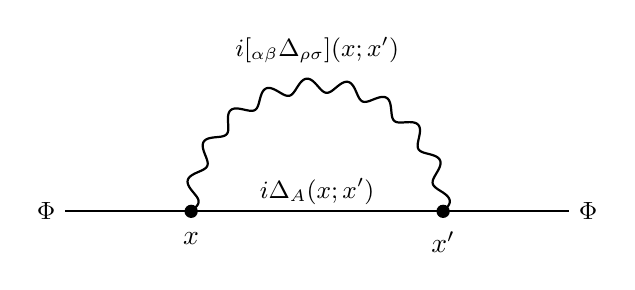
\begin{tikzpicture}[scale=1.0]
\draw[thick] (-3.2,0) -- (3.2,0);
\draw[thick, domain=0:180, samples=500, smooth, variable=\t]
  plot ({(1.6+0.09*sin(20*\t))*cos(\t)}, {(1.6+0.09*sin(20*\t))*sin(\t)});
\fill (-1.6,0) circle (2.4pt) node[below=4pt] {$x$};
\fill (1.6,0) circle (2.4pt) node[below=4pt] {$x'$};
\node[right] at (3.2,0) {\small $\Phi$};
\node[left] at (-3.2,0) {\small $\Phi$};
\node at (0,0.25) {\small $i\Delta_A(x;x')$};
\node at (0,2.05) {\small $i[{}_{\alpha\beta}\Delta_{\rho\sigma}](x;x')$};
\end{tikzpicture}
\caption{Topology of the 3-point contribution (our drawing of the content of Fig.~2 of \PI): the scalar line passes through the
two 3-point vertices at $x$ and $x'$, the graviton propagator connects them. The outer legs carry the background field $\Phi$.}
\label{fig:ch3-diagram}
\end{figure}

\paragraph{Inputs.}
\begin{itemize}[leftmargin=30pt,labelsep=5pt]
\item[(G1)] Derived Table~I and normalization \tD{} (Task~2, Chapter~1):
\begin{equation}
\begin{gathered}
\kappa\mathcal L^{(1)}=\frac12\cdot\frac1i\sum_{I=1}^2\Big[V_I^{\alpha\beta}\phi_1\phi_2\Big]_{\phi_1=\phi_2=\phi}h_{\alpha\beta},\\
V_1^{\alpha\beta}=i\kappa a^{D-2}\partial_1^\alpha\partial_2^\beta,\qquad V_2^{\alpha\beta}=-\tfrac i2\kappa a^{D-2}\eta^{\alpha\beta}\partial_1\!\cdot\partial_2 .
\end{gathered}
\label{eq:ch3-G1}
\end{equation}
\item[(G2)] Propagators \tP\,\tA:
\begin{itemize}
\item $\langle T\phi(x)\phi(x')\rangle=i\Delta_A(x;x')$. This is the Feynman propagator of the kinetic term $-\tfrac12a^{D-2}\partial\phi\cdot\partial\phi$
and satisfies \eqI{12}--\eqI{13}.
\item $\langle T\,h_{\alpha\beta}(x)h_{\rho\sigma}(x')\rangle=i[{}_{\alpha\beta}\Delta_{\rho\sigma}](x;x')$, \PI{} \eqI{20} and \eqI{25}.
\end{itemize}
Because of bosonic time ordering both propagators are symmetric under exchange:
\begin{equation*}
i\Delta_A(x;x')=i\Delta_A(x';x),\qquad i[{}_{\alpha\beta}\Delta_{\rho\sigma}](x;x')=i[{}_{\rho\sigma}\Delta_{\alpha\beta}](x';x).
\end{equation*}
\item[(G3)] Definition of $M^2$ and the effective action \tP\,\tA{} (Task~3, Chapter~2): \PI{} \eqI{168} and
\begin{equation*}
-iM^2(x;x')=\frac{\delta^2(i\Gamma_1)}{\delta\Phi(x)\,\delta\Phi(x')},\qquad e^{i\Gamma[\Phi]}=\int[Dh][D\varphi]_{\rm 1PI}\,e^{iS[\Phi+\varphi,h]}.
\end{equation*}
\end{itemize}

\paragraph{Scope.}
The substitution of the graviton propagator, i.e.\ \eqI{47}--\eqI{49} and beyond, is not part of Task~6 (it is Task~7). $D$ is general.
The singular products of propagators at $x=x'$ are defined as distributions in dimensional regularization for general $D$;
the equalities below hold in this sense, i.e.\ when integrated against test functions.

% -----------------------------------------------------------------------------------
\subsection{Effective action for the 3-point contribution \tD}

\paragraph{Background split and the cross term.}
Write $\phi=\Phi+\varphi$, with $\Phi$ the background and $\varphi$ the quantum field. Expanding the bracket in \eqref{eq:ch3-G1} produces three
kinds of terms: $\Phi\Phi h$, $\Phi\varphi h$ and $\varphi\varphi h$. Once contracted into $h_{\alpha\beta}$, the cross term can be written using the
$1\leftrightarrow2$ symmetry of $V_I$:
\begin{equation}
\big[V_I^{\alpha\beta}(\partial_1,\partial_2)\big(\Phi_1\varphi_2+\varphi_1\Phi_2\big)\big]h_{\alpha\beta}=2\big[V_I^{\alpha\beta}(\partial_1,\partial_2)\Phi_1\varphi_2\big]h_{\alpha\beta}.
\label{eq:ch3-cross}
\end{equation}
For $V_1$ this follows from $\partial_2^\alpha\partial_1^\beta h_{\alpha\beta}=\partial_1^\alpha\partial_2^\beta h_{\alpha\beta}$; $V_2$ is manifestly symmetric. Hence
\begin{equation}
S_3^{\times}=\int d^Dz\,\frac1i\sum_I\big[V_I^{\alpha\beta}(\partial_1,\partial_2)\,\Phi_1\varphi_2\big]h_{\alpha\beta}
\qquad(\text{leg 1 = outer }\Phi,\ \text{leg 2 = inner }\varphi).
\label{eq:ch3-S3x}
\end{equation}

\paragraph{Second order.}
Take $i\Gamma\supset\tfrac12\langle(iS_{\rm int})^2\rangle_{\rm c}$. The terms that are quadratic in $\Phi$ and of order $\kappa^2$ are:
\begin{enumerate}[leftmargin=18pt]
\item $\langle(iS_3^\times)^2\rangle$, with $\varphi\varphi$ and $hh$ contracted. This is Fig.~2; it is 1PI.
\item $\Phi\Phi h$ at one vertex and $\varphi\varphi h$ at the other: the graviton line ends on a scalar loop. This diagram is 1PR and is excluded.
\item $\Phi\Phi h$ together with the $\langle h\rangle$ tadpole: 1PR, excluded.
\end{enumerate}
The 4-point contribution was treated in Task~3. With \eqref{eq:ch3-S3x} and (G2),
\begin{equation*}
i\Gamma_{\rm 3pt}[\Phi]=\tfrac12\,i^2\Big(\frac1i\Big)^2\sum_{I,J}\iint d^Dz\,d^Dz'\,\big[V_I^{\alpha\beta}(z)\Phi_1\varphi_2\big]\big[V_J^{\rho\sigma}(z')\Phi_1\varphi_2\big]\;
\langle\varphi(z)\varphi(z')\rangle\,\langle h_{\alpha\beta}(z)h_{\rho\sigma}(z')\rangle .
\end{equation*}
Since $i^2(1/i)^2=1$,
\begin{equation}
\boxed{\;i\Gamma_{\rm 3pt}[\Phi]=\tfrac12\sum_{I,J}\iint d^Dz\,d^Dz'\;V_I^{\alpha\beta}(z)\,V_J^{\rho\sigma}(z')\;\Phi(z)\,\Phi(z')\;
i[{}_{\alpha\beta}\Delta_{\rho\sigma}](z;z')\;i\Delta_A(z;z')\;}
\label{eq:ch3-Gamma3}
\end{equation}
Here $\partial_1$ and $\partial'_1$ act on $\Phi(z)$ and $\Phi(z')$, while $\partial_2$ and $\partial'_2$ act on the first and second argument of $i\Delta_A$, respectively.

% -----------------------------------------------------------------------------------
\subsection{Derivation of Eq. (I.45) \tD}

\paragraph{Functional derivative and normalization.}
By (G3), $-iM^2_{\rm 3pt}(x;x')=\delta^2(i\Gamma_{\rm 3pt})/\delta\Phi(x)\delta\Phi(x')$. There are two assignments,
$(z\to x,\ z'\to x')$ and $(z\to x',\ z'\to x)$. Because of the exchange symmetry in (G2), the integrand of \eqref{eq:ch3-Gamma3} is symmetric
under $(z,I,\alpha\beta)\leftrightarrow(z',J,\rho\sigma)$, so the two assignments contribute equally. Table~\ref{tab:ch3-norm} collects all factors.

\begin{table}[h]
\centering
\begin{tabular}{lcl}
\toprule
Factor & Value & Origin\\
\midrule
cumulant expansion & $\tfrac12$ & $\tfrac12\langle(iS)^2\rangle$\\
cross term (each vertex) & $2\times2$ & Eq.~\eqref{eq:ch3-cross}\\
normalization & $(1/2i)^2$ & (G1)\\
vertex rule & $i^2$ & $e^{iS}$\\
assignments in $\delta^2$ & $2$ & $z\leftrightarrow z'$ symmetry\\
\midrule
\textbf{total} & $\mathbf{1}$ & $\tfrac12\cdot4\cdot(-\tfrac14)\cdot(-1)\cdot2=1$\\
\bottomrule
\end{tabular}
\caption{Normalization of the 3-point contribution (Task 6).}
\label{tab:ch3-norm}
\end{table}

\paragraph{Derivative rules.}
At vertex $z$, for an outer-leg derivative $\partial_{1\mu}\Phi(z)$ the functional derivative $\delta/\delta\Phi(x)$ produces $\partial^z_\mu\delta^D(z-x)$.
A partial integration in $z$ gives
\begin{equation}
\int d^Dz\;\partial^z_\mu\delta^D(z-x)\;\mathcal G(z,\ldots)=-\partial^x_\mu\,\mathcal G(x,\ldots),
\label{eq:ch3-ibp}
\end{equation}
where $\mathcal G$ is everything else that depends on $z$: $a^{D-2}(z)$, $i[\Delta](z;z')$ and $\partial_2i\Delta_A(z;z')$. The same holds at vertex $z'$.
Four rules follow:
\begin{itemize}[leftmargin=14pt]
\item \textbf{(R1)} $\partial_1\to-\partial$, acting on \emph{everything} at vertex $x$. \textbf{(R1$'$)} $\partial'_1\to-\partial'$, acting on everything at vertex $x'$.
\item \textbf{(R2)} $\partial_2\to+\partial$, acting only on $i\Delta_A(x;x')$. \textbf{(R2$'$)} $\partial'_2\to+\partial'$, acting only on $i\Delta_A$.
\end{itemize}
The product of the two outer signs is $(-1)(-1)=+1$. Therefore
{\chIIIhtag{I45}%
\begin{equation}
\boxed{\;-iM^2_{\rm 3pt}(x;x')=\sum_{I=1}^2V_I^{\alpha\beta}(x)\sum_{J=1}^2V_J^{\rho\sigma}(x')\;i[{}_{\alpha\beta}\Delta_{\rho\sigma}](x;x')\;i\Delta_A(x;x')\;}
\tag{I.45}\label{eq:ch3-45}
\end{equation}
}
with the derivatives read according to (R1)--(R2$'$) (definition sign). This is identical with \PI's \eqI{45} and with the rule stated in its text,
``partially integrate any derivative that acts upon an outer leg'' \chIIIok.

% -----------------------------------------------------------------------------------
\subsection{Comparison with the 4-point rule: the relative sign}
\label{sec:ch3-relsign}

\begin{table}[h]
\centering\small
\begin{tabular}{p{0.2\textwidth}p{0.34\textwidth}p{0.36\textwidth}}
\toprule
 & 3-point (this task) & 4-point (Task 3)\\
\midrule
position of outer legs & different vertices: $x$ and $x'$ & same vertex $x$, with $\delta^D(x-x')$\\
leg 1 & partial integration: $-\partial$, on everything & partial integration: $-\partial$, on everything\\
leg 2 & partial integration: $-\partial'$, on everything & $+\partial$ on $\delta^D(x-x')$ with respect to $x$ $(=-\partial')$\\
sign product & $(-)(-)=+$ & $(-)(+)=-$\\
paper's rule & $(-)(-)$ \chIIIok & \eqI{32}: $\partial_2\to+\partial'$, i.e.\ $(-)(-)$ \chIIIno\\
\bottomrule
\end{tabular}
\caption{Derivative rules for the outer legs in the 3-point and 4-point contributions (Task 6).}
\label{tab:ch3-rules}
\end{table}

In the 4-point contribution, once the first $\delta^D(z-x)$ has been integrated no $z$ is left for a second partial integration.
The remaining derivative acts on $\delta^D(x-x')$ with respect to the vertex coordinate $x$. In \eqI{32} the paper treats this case with
the same sign as the 3-point rule. At the end of Task~6 this was read as confirming the preliminary note of Task~3: in the paper's total result,
the 4-point contribution enters with the opposite sign relative to the 3-point contribution. (As explained in the note at the beginning of
this section, Task~9 later showed that the paper's 3-point contribution is reversed as well, from \eqI{47} on, so that the relative sign in the
paper is in fact consistent.)

% -----------------------------------------------------------------------------------
\subsection{Derivation of Eq. (I.46) \tD}

The four $(I,J)$ terms of \eqref{eq:ch3-45} are expanded with \eqref{eq:ch3-G1}. In $V_1$ it does not matter which index goes to the outer leg,
because $i[{}_{\alpha\beta}\Delta_{\rho\sigma}]$ is symmetric within the pair $\alpha\beta$. The factor $(aa')^{D-2}=a^{D-2}(x)\,a^{D-2}(x')$ belongs to the
``everything'' on which the outer derivatives act. Indices are moved with $\eta$; for example $\partial^\alpha X_{\alpha\ldots}=\partial_\alpha X^\alpha{}_{\ldots}$.
In $V_2$ we write $\partial_1\!\cdot\partial_2=\partial_1^\mu\partial_{2\mu}$ and apply (R1), $\partial_1^\mu\to-\partial^\mu$, and (R2), $\partial_{2\mu}\to\partial_\mu$.
Table~\ref{tab:ch3-IJ} shows the bookkeeping ($I$ refers to the vertex at $x$, $J$ to the vertex at $x'$).

\begin{table}[h]
\centering\small
\renewcommand{\arraystretch}{1.25}
\begin{tabular}{clllll}
\toprule
$(I,J)$ & $V$ coefficients & outer derivatives & contraction & inner & result\\
\midrule
(1,1) & $(i\kappa)(i\kappa)=-\kappa^2$ & $(-\partial^\alpha)(-\partial'^\rho)$ & $i[{}^{\alpha\beta}\Delta^{\rho\sigma}]$ & $\partial_\beta\partial'_\sigma$ & $-\kappa^2\partial_\alpha\partial'_\rho\{\ldots\}$\\
(2,1) & $(-\tfrac i2\kappa)(i\kappa)=+\tfrac{\kappa^2}2$ & $(-\partial^\mu)(-\partial'^\rho)$ & $\eta^{\alpha\beta}\to i[{}^\alpha_\alpha\Delta^{\rho\sigma}]$ & $\partial_\mu\partial'_\sigma$ & $+\tfrac{\kappa^2}2\partial^\mu\partial'_\rho\{\ldots\}$\\
(1,2) & $(i\kappa)(-\tfrac i2\kappa)=+\tfrac{\kappa^2}2$ & $(-\partial^\alpha)(-\partial'^\nu)$ & $\eta^{\rho\sigma}\to i[{}^{\alpha\beta}\Delta^\rho{}_\rho]$ & $\partial_\beta\partial'_\nu$ & $+\tfrac{\kappa^2}2\partial_\alpha\partial'^\nu\{\ldots\}$\\
(2,2) & $(-\tfrac i2\kappa)^2=-\tfrac{\kappa^2}4$ & $(-\partial^\mu)(-\partial'^\nu)$ & $i[{}^\alpha_\alpha\Delta^\rho{}_\rho]$ & $\partial_\mu\partial'_\nu$ & $-\tfrac{\kappa^2}4\partial^\mu\partial'^\nu\{\ldots\}$\\
\bottomrule
\end{tabular}
\caption{The four $(I,J)$ terms of \eqref{eq:ch3-45} (Task 6). ``Inner'' lists the derivatives that act only on $i\Delta_A$.}
\label{tab:ch3-IJ}
\end{table}

\noindent Summing the four rows:
{\chIIIhtag{I46}%
\begin{equation}
\boxed{\;
\begin{aligned}
-iM^2_{\rm 3pt}(x;x')={}&-\kappa^2\partial_\alpha\partial'_\rho\Big\{(aa')^{D-2}\,i[{}^{\alpha\beta}\Delta^{\rho\sigma}](x;x')\,\partial_\beta\partial'_\sigma i\Delta_A(x;x')\Big\}\\
&+\frac{\kappa^2}2\partial^\mu\partial'_\rho\Big\{(aa')^{D-2}\,i[{}^\alpha_\alpha\Delta^{\rho\sigma}](x;x')\,\partial_\mu\partial'_\sigma i\Delta_A(x;x')\Big\}\\
&+\frac{\kappa^2}2\partial_\alpha\partial'^\nu\Big\{(aa')^{D-2}\,i[{}^{\alpha\beta}\Delta^\rho{}_\rho](x;x')\,\partial_\beta\partial'_\nu i\Delta_A(x;x')\Big\}\\
&-\frac{\kappa^2}4\partial^\mu\partial'^\nu\Big\{(aa')^{D-2}\,i[{}^\alpha_\alpha\Delta^\rho{}_\rho](x;x')\,\partial_\mu\partial'_\nu i\Delta_A(x;x')\Big\}
\end{aligned}\;}
\tag{I.46}\label{eq:ch3-46}
\end{equation}
}
(definition sign). All coefficients are independent of $D$; $D$ appears only through $(aa')^{D-2}$ and inside the propagators.

% -----------------------------------------------------------------------------------
\subsection{Independent analytic cross-checks}

\paragraph{Textbook comparison \tA\,\tC.}
In the cubic theory $\mathcal L_{\rm int}=\tfrac g2\phi^2\chi$, the normalization used here gives the vertex $V=2i\cdot\tfrac g2=ig$. The one-loop $\phi$
self-energy is, by the standard result, $V^2\times\Delta_\phi\times\Delta_\chi$ with symmetry factor $1$. This is the same normalization as in \eqref{eq:ch3-45}.

\paragraph{Consistency with the flat-space limit (observation).}
The flat-space 3-point expression in \PI's \eqI{175}\footnote{The Task~6 report cites this expression as (174). In the printed paper
(p.~124005-15, right column) \eqI{174} is the flat-space limit of the 4-point contribution, and the flat-space 3-point expression is \eqI{175};
the reference has been corrected here.} has the same structure and the same signs as \eqI{46} ($-\kappa^2$, $+\tfrac{\kappa^2}2$, $+\tfrac{\kappa^2}2$,
$-\tfrac{\kappa^2}4$). This shows that \eqI{46} is used consistently within the paper.

% -----------------------------------------------------------------------------------
\subsection{Code checks \tC}
\label{sec:ch3-t6-code}

The script \chIIIcode{check\_45\_46.py} (SymPy and mpmath; about 3 minutes) performs three checks. It does not replace the analytic derivation above.
\begin{itemize}[leftmargin=14pt]
\item \textbf{(a) Index algebra.}
Set-up: $D=3$; a generic tensor $X_{\alpha\beta\rho\sigma}(x;x')$, symmetric within each pair, with 36 independent components
(no pair-exchange symmetry is assumed, since $x\ne x'$); derivatives represented by formal vectors ($P,P'$ outer, $Q,Q'$ inner).
With (R1)--(R2$'$), $\sum_{IJ}V_IV_JX$ is identical to \eqI{46}: \texttt{True} \chIIIok.
With $V_1\to-V_1$, i.e.\ with the printed left-hand side of \eqI{7}, the identity fails; the difference is exactly the sign reversal of the
2nd and 3rd terms (\texttt{difference = -2*(t2+t3): True}).
\item \textbf{(b) Normalization.} $\tfrac12\cdot2\cdot2\cdot(1/2i)^2\cdot i^2\cdot2=1$ \chIIIok.
\item \textbf{(c) Derivative rules with test functions.}
Set-up: a one-dimensional toy model, $i\Gamma=\tfrac12\iint W(z,z')\Phi'(z)\Phi'(z')$, with $W$ built from explicit smooth symmetric kernels,
\begin{equation*}
\begin{gathered}
W=C(z)\,C(z')\,G(z,z')\,\partial_z\partial_{z'}\Delta_\ell(z,z'),\\
C(u)=1+u^2,\qquad G=(1+zz')\,e^{-(z-z')^2/2},\qquad \Delta_\ell=e^{-(z-z')^2},
\end{gathered}
\end{equation*}
where $C$ plays the role of $a^{D-2}$, $G$ that of the graviton propagator and $\Delta_\ell$ that of the scalar propagator; the test functions are
$f_1=e^{-z^2}$ and $f_2=z\,e^{-(z-1)^2}$.
The Gateaux second derivative is $0.779492709611$; the kernel of the rule of \eqI{45}, $(-\partial_z)(-\partial_{z'})$ acting on everything, gives the
same value \chIIIok. A rule that takes one outer leg with the opposite sign (the type of rule used in \eqI{32}) gives $-0.779492709611$ \chIIIno.
\end{itemize}
Output (re-run for these notes; identical with the output recorded in Task~6):
{\footnotesize
\begin{verbatim}
== (a) index algebra (45) -> (46), D=3, generic within-pair-symmetric X_{ab rs}(x;x') ==
  Sum_IJ V_I(x) V_J(x') X  ==  (46)  with derived V_1 = +i kappa ...  : True
  with the sign of (7)'s printed LHS (V_1 = -i kappa ...)            : False
                                       (difference = -2*(t2+t3): True )
== (b) normalization: (1/2) * 2 * 2 * (1/2i)^2 * i^2 * 2 ==
  factor = 1
== (c) derivative rules, 1D toy with explicit smooth kernels and test functions ==
  Gateaux  d^2(i Gamma)/de1 de2 = 0.779492709611
  (45) rule  int f1 K f2        = 0.779492709611   equal: True
  one outer leg with + sign     = -0.779492709611   equal: False
\end{verbatim}
}
\noindent(The third line of (a) is wrapped here; the script prints it as one line.)

% -----------------------------------------------------------------------------------
\subsection{Comparison with the paper}
\label{sec:ch3-t6-compare}

\begin{table}[h]
\centering\small
\renewcommand{\arraystretch}{1.2}
\begin{tabular}{p{0.3\textwidth}p{0.42\textwidth}p{0.12\textwidth}c}
\toprule
Item & Derived & Paper & \\
\midrule
\eqI{45}: normalization & $1$ (Table~\ref{tab:ch3-norm}) & $1$ & \chIIIok\\
\eqI{45}: structure $V(x)V(x')\,i[\Delta](x;x')$ $\times\,i\Delta_A(x;x')$ & Eq.~\eqref{eq:ch3-45} & same & \chIIIok\\
outer-leg rule & $-\partial$ (on everything), at both vertices & ``partially integrate'' & \chIIIok\\
inner-leg rule & $+\partial$, only on $i\Delta_A$ & same & \chIIIok\\
\eqI{46}, 1st term & $-\kappa^2\partial_\alpha\partial'_\rho\{\ldots i[{}^{\alpha\beta}\Delta^{\rho\sigma}]\ldots\}$ & same & \chIIIok\\
\eqI{46}, 2nd term & $+\tfrac{\kappa^2}2\partial^\mu\partial'_\rho\{\ldots i[{}^\alpha_\alpha\Delta^{\rho\sigma}]\ldots\}$ & same & \chIIIok\\
\eqI{46}, 3rd term & $+\tfrac{\kappa^2}2\partial_\alpha\partial'^\nu\{\ldots i[{}^{\alpha\beta}\Delta^\rho{}_\rho]\ldots\}$ & same & \chIIIok\\
\eqI{46}, 4th term & $-\tfrac{\kappa^2}4\partial^\mu\partial'^\nu\{\ldots i[{}^\alpha_\alpha\Delta^\rho{}_\rho]\ldots\}$ & same & \chIIIok\\
\bottomrule
\end{tabular}
\caption{Task 6: comparison with \PI.}
\label{tab:ch3-t6-comp}
\end{table}

\begin{resultbox}[Conclusion (Task 6)]
\eqI{45} and \eqI{46} agree exactly with the derivation; there is no discrepancy.
The printed \eqI{46} is consistent with the derived $V_1=+i\kappa\ldots$. This agrees with the finding of Task~2: the $-\tfrac12\kappa$ on the
left-hand side of \eqI{7} is only a typographical error.
\end{resultbox}

\paragraph{Consequence of the relative sign (as assessed in Task 6).}
The paper's 3-point rule agrees with the definitions; its 4-point rule \eqI{32} does not (Sec.~\ref{sec:ch3-relsign}). Accordingly, in the paper's sum
$-iM^2=-iM^2_{\rm 4pt}+(-iM^2_{\rm 3pt})+(\text{counterterms})$, \eqI{44} appears with the opposite of its correct sign.
Task~6 proposed to determine the effect on the renormalized result as follows: multiply the paper's \eqI{44} by $-1$ (and drop the $\mp2$ terms that
originate from \eqI{40}), then redo the 3-point contributions and the counterterm adjustment of Part~IV. According to Task~5, the terms
$3\ln(aa')a^D\square$, $-4\ln(aa')a^{D-2}\nabla^2$ and $9H^2a^D$ are not of counterterm form; the sign could therefore affect the final finite result.
(This plan was overtaken by Tasks~7 and~9; see the note at the start of this section.)

\paragraph{Accumulated findings (Tasks 2--6).}
Identifiers in parentheses (S$n$, B$n$, C$n$) refer to the classified list of findings in Chapter~\ref{ch:summary}.
\begin{center}\small
\renewcommand{\arraystretch}{1.2}
\begin{tabular}{p{0.16\textwidth}p{0.4\textwidth}p{0.36\textwidth}}
\toprule
Location & Finding & Effect\\
\midrule
\eqI{7}, left side (C3) & $-\tfrac12\kappa$ printed, correct is $+\tfrac12\kappa$ & none; \eqI{46} was built with the correct $V_1$\\
Table II, $U_2$ (C5) & $-\tfrac i4$ printed, correct is $+\tfrac i4$ & none; \eqI{33} was built with the correct value\\
\eqI{32}--\eqI{33} (S1) & overall sign reversed because of the $\partial_2$ rule & at the time: \emph{confirmed} that the 4-point contribution enters with the opposite sign relative to the 3-point one (later revised, see above)\\
\eqI{39} (C6) & $\bar\eta_{\rho\sigma}\to\bar\eta^{\rho\sigma}$ & none\\
\eqI{40} (B1) & finite part $+2$ printed, correct is $-2$ & carried into \eqI{41} and \eqI{44}; absorbable into counterterms\\
\eqI{41}$\to$\eqI{44} & algebra of \eqI{42}--\eqI{43} correct & ---\\
\eqI{45}--\eqI{46} & exact agreement & ---\\
\bottomrule
\end{tabular}
\end{center}

% -----------------------------------------------------------------------------------
\subsection{Calculation record (Task 6)}
\begin{itemize}[leftmargin=14pt]
\item \textbf{Derived.} Background split and cross term, Eqs.~\eqref{eq:ch3-cross}--\eqref{eq:ch3-S3x}.
The 3-point effective action \eqref{eq:ch3-Gamma3}; the reason for excluding the 1PR contributions.
Normalization table (Table~\ref{tab:ch3-norm}). Outer- and inner-leg derivative rules \eqref{eq:ch3-ibp} and (R1)--(R2$'$).
\eqI{45} [Eq.~\eqref{eq:ch3-45}]. The origin of the sign difference between the 3- and 4-point rules (Sec.~\ref{sec:ch3-relsign}).
\eqI{46} [Eq.~\eqref{eq:ch3-46}]: the four $(I,J)$ terms with explicit coefficients and contractions.
\item \textbf{Checks passed.} Textbook normalization; SymPy/mpmath (a) index algebra, (b) normalization, (c) derivative rule with test
functions (\chIIIcode{check\_45\_46.py}). All were actually run.
\item \textbf{Discrepancies.} None in \eqI{45} and \eqI{46}.
\item \textbf{Point established in Task 6.} In \PI{} the 4-point and 3-point contributions are built with different derivative rules; the 4-point
contribution is reversed (with respect to the definitions). \emph{Later revision:} Task~9 showed that the 3-point contribution is reversed as well,
through \eqI{47}--\eqI{49}, so the relative sign is consistent.
\item \textbf{Open point (at the time).} The effect on the renormalized result; to be checked in the continuation of the 3-point computation and in Part~IV.
\end{itemize}

% ===================================================================================
\section{Task 7: inserting the graviton propagator, Eqs. (I.47)--(I.49)}
\label{sec:ch3-task7}
% ===================================================================================

\begin{discbox}[Summary of findings (Task 7)]
\begin{itemize}[leftmargin=12pt]
\item All nine terms of \eqI{47}--\eqI{49} were derived. Their structures, the $D$-dependent coefficients $\tfrac{D-1}{D-3}$ and $\tfrac{2(D-2)}{D-3}$,
and the magnitudes agree with the paper.
\item \textbf{The overall sign is reversed in all nine terms:} the derived \eqI{47}--\eqI{49} are exactly $-1$ times the printed ones.
The result was obtained along two independent routes: from the paper's \eqI{46}, and directly from \eqI{45} with Table~I.
Hence the printed \eqI{47}--\eqI{49} are inconsistent with the paper's own \eqI{46}.
\item In the $AA$ sector an extra pair of the form $\partial_i\partial'_j\{\ldots(\partial_i\partial'_j-\partial_j\partial'_i)i\Delta_A\}$ appears at an intermediate step.
It vanishes identically because of the spatial homogeneity of $i\Delta_A$ ($\partial'_ii\Delta_A=-\partial_ii\Delta_A$). The paper does not write it either.
\item \textbf{Significance.} If the signs of \eqI{47}--\eqI{49} were used in the subsequent steps, the paper's 3-point contribution is, like the
4-point contribution, reversed overall. The relative sign of the two contributions is then consistent, but the overall sign of the bare $M^2$ is
opposite to the convention of \eqI{168} and \eqI{131}. This was to be checked with Table~III and beyond (it was, in Task~9: see Sec.~\ref{sec:ch3-t7-assess}).
\end{itemize}
\end{discbox}

% -----------------------------------------------------------------------------------
\subsection{Goal, inputs, scope and notation}

\paragraph{Targets \tP.}
\PI, p.~124005-5 (introductory sentence in the left column, equations in the right column; all symbols legible), prints, with the paper's square brackets:
\begin{align}
&\kappa^2\nabla\!\cdot\!\nabla'\big[(aa')^{D-2}i\Delta_A\nabla\!\cdot\!\nabla'i\Delta_A\big]-\kappa^2\Big(\frac{D-1}{D-3}\Big)\partial_0\partial'_0\big[(aa')^{D-2}i\Delta_A\partial_0\partial'_0i\Delta_A\big]\notag\\
&\quad+\kappa^2\partial_i\partial'_0\big[(aa')^{D-2}i\Delta_A\partial_i\partial'_0i\Delta_A\big]+\kappa^2\partial_0\partial'_i\big[(aa')^{D-2}i\Delta_A\partial_0\partial'_ii\Delta_A\big],
\tag*{\eqI{47}}\\[3pt]
&-\kappa^2\partial_0\partial'_0\big[(aa')^{D-2}i\Delta_B\nabla\!\cdot\!\nabla'i\Delta_A\big]-\kappa^2\partial_i\partial'_0\big[(aa')^{D-2}i\Delta_B\partial_0\partial'_ii\Delta_A\big]\notag\\
&\quad-\kappa^2\partial_0\partial'_i\big[(aa')^{D-2}i\Delta_B\partial_i\partial'_0i\Delta_A\big]-\kappa^2\nabla\!\cdot\!\nabla'\big[(aa')^{D-2}i\Delta_B\partial_0\partial'_0i\Delta_A\big],
\tag*{\eqI{48}}\\[3pt]
&2\kappa^2\Big(\frac{D-2}{D-3}\Big)\partial_0\partial'_0\big[(aa')^{D-2}i\Delta_C\partial_0\partial'_0i\Delta_A\big].
\tag*{\eqI{49}}
\end{align}
These expressions were not used as input in the derivation; they enter only in the comparison of Sec.~\ref{sec:ch3-t7-compare}.

\paragraph{Inputs.}
\begin{itemize}[leftmargin=30pt,labelsep=5pt]
\item[(G1)] The derived \eqI{46} \tD{} (Task~6, Eq.~\eqref{eq:ch3-46}). Outer derivatives ($\partial,\partial'$) act on everything, inner derivatives only on $i\Delta_A$:
\begin{equation}
\begin{aligned}
-iM^2_{\rm 3pt}={}&-\kappa^2\partial_\alpha\partial'_\rho\{(aa')^{D-2}X^{\alpha\beta\rho\sigma}\partial_\beta\partial'_\sigma i\Delta_A\}
+\tfrac{\kappa^2}2\partial^\mu\partial'_\rho\{(aa')^{D-2}X^\alpha{}_\alpha{}^{\rho\sigma}\partial_\mu\partial'_\sigma i\Delta_A\}\\
&+\tfrac{\kappa^2}2\partial_\alpha\partial'^\nu\{(aa')^{D-2}X^{\alpha\beta\rho}{}_\rho\partial_\beta\partial'_\nu i\Delta_A\}
-\tfrac{\kappa^2}4\partial^\mu\partial'^\nu\{(aa')^{D-2}X^\alpha{}_\alpha{}^\rho{}_\rho\partial_\mu\partial'_\nu i\Delta_A\},
\end{aligned}
\label{eq:ch3-t7G1}
\end{equation}
with $X^{\alpha\beta\rho\sigma}\equiv i[{}^{\alpha\beta}\Delta^{\rho\sigma}](x;x')$.
\item[(G2)] The graviton propagator \tP, \eqI{20}--\eqI{24}: $X_{\alpha\beta\rho\sigma}=\sum_{I=A,B,C}T^I_{\alpha\beta\rho\sigma}\,i\Delta_I(x;x')$ with
\begin{equation}
\begin{aligned}
&T^A_{\alpha\beta\rho\sigma}=2\bar\eta_{\alpha(\rho}\bar\eta_{\sigma)\beta}-\tfrac{2}{D-3}\bar\eta_{\alpha\beta}\bar\eta_{\rho\sigma},\qquad
T^B_{\alpha\beta\rho\sigma}=-4\delta^0_{(\alpha}\bar\eta_{\beta)(\rho}\delta^0_{\sigma)},\\
&T^C_{\alpha\beta\rho\sigma}=\tfrac{2}{(D-2)(D-3)}\big[(D-3)\delta^0_\alpha\delta^0_\beta+\bar\eta_{\alpha\beta}\big]\big[(D-3)\delta^0_\rho\delta^0_\sigma+\bar\eta_{\rho\sigma}\big].
\end{aligned}
\label{eq:ch3-T}
\end{equation}
The $T^I$ are constant tensors; therefore $i\Delta_I(x;x')$ stays inside the bracket on which the outer derivatives act.
\item[(G3)] Tensor tools \tD{} (Task~4, Chapter~2): $u_\mu=\delta^0_\mu$, $u^\mu=-\delta^\mu_0$, $\bar\eta_{\mu\nu}=\eta_{\mu\nu}+u_\mu u_\nu$.
For vectors $V,W$: $u\cdot V=-V_0$ and $\bar\eta_{\mu\nu}V^\mu W^\nu=\bar V\!\cdot\!\bar W\equiv\sum_iV_iW_i$. Traces:
\begin{equation}
\begin{aligned}
&\eta^{\alpha\beta}T^A_{\alpha\beta\mu\nu}=-\tfrac{4}{D-3}\bar\eta_{\mu\nu},\qquad \eta^{\alpha\beta}T^B_{\alpha\beta\mu\nu}=0,\qquad \eta^{\alpha\beta}T^C_{\alpha\beta\mu\nu}=\tfrac{4}{(D-2)(D-3)}f_{\mu\nu},\\
&\eta^{\alpha\beta}\eta^{\rho\sigma}T^{A,B,C}_{\alpha\beta\rho\sigma}=-\tfrac{4(D-1)}{D-3},\ \ 0,\ \ \tfrac{8}{(D-2)(D-3)},
\end{aligned}
\label{eq:ch3-traces}
\end{equation}
where $f_{\mu\nu}\equiv(D-3)u_\mu u_\nu+\bar\eta_{\mu\nu}$.
\item[(G4)] Homogeneity of $i\Delta_A$ \tP\,\tD: by \eqI{11} and \eqI{13}, $i\Delta_A=A(y)+k\ln(aa')$, which depends on $\vec x,\vec x'$ only through $\|\vec x-\vec x'\|$. Hence
\begin{equation}
\partial'_i\,i\Delta_A=-\partial_i\,i\Delta_A,\qquad \partial_i\partial'_j\,i\Delta_A=\partial_j\partial'_i\,i\Delta_A .
\label{eq:ch3-hom}
\end{equation}
\end{itemize}

\paragraph{Scope and notation.}
Eq.~\eqI{50} and beyond (the $y$ representation and the local/logarithm/normal split) are not part of Task~7. $D$ is general; at no step is $D=4$ set.
As a shorthand we write
\begin{equation}
\chIIIbr{\partial_a\partial'_c}{\partial_b\partial'_d}{I}\equiv\partial_a\partial'_c\Big\{(aa')^{D-2}\,i\Delta_I(x;x')\,\partial_b\partial'_d\,i\Delta_A(x;x')\Big\}.
\label{eq:ch3-bracket}
\end{equation}
The derivatives on the left of the bar are outer, those on the right inner. During the computation the outer derivatives are represented by $P,P'$ and the
inner ones by $Q,Q'$; for example $P_0P'_0(\bar Q\!\cdot\!\bar Q')\to\chIIIbr{\partial_0\partial'_0}{\nabla\!\cdot\!\nabla'}{}$.

% -----------------------------------------------------------------------------------
\subsection{Term-by-term contractions \tD}

(G2) is inserted into the four terms of \eqref{eq:ch3-t7G1}. We use $T_I^{\alpha\beta\rho\sigma}P_\alpha Q_\beta P'_\rho Q'_\sigma=T^I_{\alpha\beta\rho\sigma}P^\alpha Q^\beta P'^\rho Q'^\sigma$ and (G3);
$P\!\cdot\!Q=-P_0Q_0+\bar P\!\cdot\!\bar Q$ is the Lorentz product.

\paragraph{First term: $-\kappa^2\,T^{\alpha\beta\rho\sigma}P_\alpha Q_\beta P'_\rho Q'_\sigma$.}
The contraction $T^I_{\alpha\beta\rho\sigma}P^\alpha Q^\beta P'^\rho Q'^\sigma$ (before multiplying by $-\kappa^2$) is
\begin{equation}
\begin{aligned}
T^A:&\quad (\bar P\!\cdot\!\bar P')(\bar Q\!\cdot\!\bar Q')+(\bar P\!\cdot\!\bar Q')(\bar P'\!\cdot\!\bar Q)-\tfrac{2}{D-3}(\bar P\!\cdot\!\bar Q)(\bar P'\!\cdot\!\bar Q'),\\
T^B:&\quad -\big[P_0Q'_0(\bar P'\!\cdot\!\bar Q)+Q_0Q'_0(\bar P\!\cdot\!\bar P')+P_0P'_0(\bar Q\!\cdot\!\bar Q')+Q_0P'_0(\bar P\!\cdot\!\bar Q')\big],\\
T^C:&\quad \tfrac{2}{(D-2)(D-3)}\big[(D-3)P_0Q_0+\bar P\!\cdot\!\bar Q\big]\big[(D-3)P'_0Q'_0+\bar P'\!\cdot\!\bar Q'\big].
\end{aligned}
\label{eq:ch3-c1}
\end{equation}
Used:
\begin{itemize}[leftmargin=14pt]
\item for $T^A$: $\bar\eta_{\alpha\rho}P^\alpha P'^\rho=\bar P\!\cdot\!\bar P'$ and similar;
\item for $T^B$: $(u\!\cdot\!P)(u\!\cdot\!Q')=P_0Q'_0$ and similar; the four terms come from expanding the symmetrization in \eqI{23};
\item for $T^C$: $f_{\alpha\beta}P^\alpha Q^\beta=(D-3)P_0Q_0+\bar P\!\cdot\!\bar Q$.
\end{itemize}

\paragraph{Second and third terms: one trace.}
\begin{equation}
\begin{aligned}
\tfrac{\kappa^2}2(P\!\cdot\!Q)\,\eta^{\alpha\beta}T_{\alpha\beta}{}^{\rho\sigma}P'_\rho Q'_\sigma:&\quad A:\ -\tfrac{2\kappa^2}{D-3}(P\!\cdot\!Q)(\bar P'\!\cdot\!\bar Q'),\qquad B:\ 0,\\
&\quad C:\ \tfrac{2\kappa^2}{(D-2)(D-3)}(P\!\cdot\!Q)\big[(D-3)P'_0Q'_0+\bar P'\!\cdot\!\bar Q'\big],\\[3pt]
\tfrac{\kappa^2}2(P'\!\cdot\!Q')\,T^{\alpha\beta}{}_{\rho}{}^{\rho}P_\alpha Q_\beta:&\quad A:\ -\tfrac{2\kappa^2}{D-3}(\bar P\!\cdot\!\bar Q)(P'\!\cdot\!Q'),\qquad B:\ 0,\\
&\quad C:\ \tfrac{2\kappa^2}{(D-2)(D-3)}\big[(D-3)P_0Q_0+\bar P\!\cdot\!\bar Q\big](P'\!\cdot\!Q').
\end{aligned}
\label{eq:ch3-c2}
\end{equation}
The trace in the third term has the same form as in the second because of the pair-exchange symmetry of the $T^I$ (Task~3).

\paragraph{Fourth term: double trace.}
\begin{equation}
-\tfrac{\kappa^2}4(P\!\cdot\!Q)(P'\!\cdot\!Q')\,\eta\eta T:\qquad A:\ +\kappa^2\tfrac{D-1}{D-3}(P\!\cdot\!Q)(P'\!\cdot\!Q'),\qquad B:\ 0,\qquad
C:\ -\tfrac{2\kappa^2}{(D-2)(D-3)}(P\!\cdot\!Q)(P'\!\cdot\!Q').
\label{eq:ch3-c3}
\end{equation}

% -----------------------------------------------------------------------------------
\subsection{Sorting by the type of scalar propagator \tD}

We abbreviate\footnote{The original report used the letters $a,\bar a,b,\bar b$ here; we rename them to avoid a clash with the scale factor $a$.
For the same reason its $A_{1,2},B_{1,2}$ and $c_0$ of the $AC$ sector are renamed $M_{1,2},N_{1,2}$ and $c_C$ below ($c_0$ is used in Task~8 for the first coefficient of \eqI{14}).}
$m\equiv P_0Q_0$, $\bar m\equiv\bar P\!\cdot\!\bar Q$, $n\equiv P'_0Q'_0$, $\bar n\equiv\bar P'\!\cdot\!\bar Q'$, so that $P\!\cdot\!Q=-m+\bar m$ and $P'\!\cdot\!Q'=-n+\bar n$.

\paragraph{$AA$ terms.}
Table~\ref{tab:ch3-AA} collects the $T^A$ parts of \eqref{eq:ch3-c1}--\eqref{eq:ch3-c3}.
\begin{table}[h]
\centering
\renewcommand{\arraystretch}{1.3}
\begin{tabular}{lccccc}
\toprule
Monomial & 1st term & 2nd term & 3rd term & 4th term & Total$/\kappa^2$\\
\midrule
$\bar m\,\bar n$ & $+\tfrac2{D-3}$ & $-\tfrac2{D-3}$ & $-\tfrac2{D-3}$ & $+\tfrac{D-1}{D-3}$ & $+1$\\
$m\,\bar n$ & --- & $+\tfrac2{D-3}$ & --- & $-\tfrac{D-1}{D-3}$ & $-1$\\
$\bar m\,n$ & --- & --- & $+\tfrac2{D-3}$ & $-\tfrac{D-1}{D-3}$ & $-1$\\
$m\,n$ & --- & --- & --- & $+\tfrac{D-1}{D-3}$ & $+\tfrac{D-1}{D-3}$\\
$(\bar P\!\cdot\!\bar P')(\bar Q\!\cdot\!\bar Q')$ & $-1$ & --- & --- & --- & $-1$\\
$(\bar P\!\cdot\!\bar Q')(\bar P'\!\cdot\!\bar Q)$ & $-1$ & --- & --- & --- & $-1$\\
\bottomrule
\end{tabular}
\caption{Coefficients of the $AA$ monomials (Task 7).}
\label{tab:ch3-AA}
\end{table}

In the first row $\tfrac{2-2-2+D-1}{D-3}=1$: the factor $D-3$ cancels exactly. The total is
\begin{equation}
\kappa^2\Big\{-(\bar P\!\cdot\!\bar P')(\bar Q\!\cdot\!\bar Q')+\tfrac{D-1}{D-3}\,mn-\bar m\,n-m\,\bar n\Big\}
+\kappa^2\Big\{\bar m\,\bar n-(\bar P\!\cdot\!\bar Q')(\bar P'\!\cdot\!\bar Q)\Big\}.
\label{eq:ch3-AAsum}
\end{equation}
The second curly bracket is $\chIIIbr{\partial_i\partial'_j}{\partial_i\partial'_j-\partial_j\partial'_i}{A}$. By (G4) the inner derivatives may be taken as
$\partial'_j=-\partial_j$; then $(\partial_i\partial'_j-\partial_j\partial'_i)i\Delta_A=-(\partial_i\partial_j-\partial_j\partial_i)i\Delta_A=0$. This pair vanishes identically.
With the mapping $\bar m\,n=P_iQ_iP'_0Q'_0\to\chIIIbr{\partial_i\partial'_0}{\partial_i\partial'_0}{}$ and $m\,\bar n=P_0Q_0P'_iQ'_i\to\chIIIbr{\partial_0\partial'_i}{\partial_0\partial'_i}{}$,
{\chIIIhtag{I47p}%
\begin{equation}
\boxed{\;
\begin{aligned}
AA:\quad&-\kappa^2\nabla\!\cdot\!\nabla'\big[(aa')^{D-2}i\Delta_A\nabla\!\cdot\!\nabla'i\Delta_A\big]\\
&+\kappa^2\Big(\frac{D-1}{D-3}\Big)\partial_0\partial'_0\big[(aa')^{D-2}i\Delta_A\partial_0\partial'_0i\Delta_A\big]\\
&-\kappa^2\partial_i\partial'_0\big[(aa')^{D-2}i\Delta_A\partial_i\partial'_0i\Delta_A\big]\\
&-\kappa^2\partial_0\partial'_i\big[(aa')^{D-2}i\Delta_A\partial_0\partial'_ii\Delta_A\big]
\end{aligned}\;}
\tag{I.47$'$}\label{eq:ch3-47}
\end{equation}
}

\paragraph{$AB$ terms.}
Since the traces of $T^B$ vanish, only the first term contributes: $-\kappa^2\times$\eqref{eq:ch3-c1}$_B$. The four monomials map as follows:
\begin{itemize}[leftmargin=14pt]
\item $P_0P'_0(\bar Q\!\cdot\!\bar Q')\to\chIIIbr{\partial_0\partial'_0}{\nabla\!\cdot\!\nabla'}{B}$;
\item $Q_0P'_0(\bar P\!\cdot\!\bar Q')\to\chIIIbr{\partial_i\partial'_0}{\partial_0\partial'_i}{B}$;
\item $P_0Q'_0(\bar P'\!\cdot\!\bar Q)\to\chIIIbr{\partial_0\partial'_i}{\partial_i\partial'_0}{B}$;
\item $Q_0Q'_0(\bar P\!\cdot\!\bar P')\to\chIIIbr{\nabla\!\cdot\!\nabla'}{\partial_0\partial'_0}{B}$.
\end{itemize}
{\chIIIhtag{I48p}%
\begin{equation}
\boxed{\;
\begin{aligned}
AB:\quad&+\kappa^2\partial_0\partial'_0\big[(aa')^{D-2}i\Delta_B\nabla\!\cdot\!\nabla'i\Delta_A\big]+\kappa^2\partial_i\partial'_0\big[(aa')^{D-2}i\Delta_B\partial_0\partial'_ii\Delta_A\big]\\
&+\kappa^2\partial_0\partial'_i\big[(aa')^{D-2}i\Delta_B\partial_i\partial'_0i\Delta_A\big]+\kappa^2\nabla\!\cdot\!\nabla'\big[(aa')^{D-2}i\Delta_B\partial_0\partial'_0i\Delta_A\big]
\end{aligned}\;}
\tag{I.48$'$}\label{eq:ch3-48}
\end{equation}
}

\paragraph{$AC$ terms.}
Define $M_1=(D-3)m+\bar m$, $M_2=-m+\bar m$, and similarly $N_1=(D-3)n+\bar n$, $N_2=-n+\bar n$. With $c_C\equiv\tfrac{2\kappa^2}{(D-2)(D-3)}$
the $C$ parts of \eqref{eq:ch3-c1}--\eqref{eq:ch3-c3} add up to
\begin{equation}
c_C\big[-M_1N_1+M_2N_1+M_1N_2-M_2N_2\big]=-c_C(M_1-M_2)(N_1-N_2)=-c_C\,(D-2)^2\,mn ,
\label{eq:ch3-ACfac}
\end{equation}
so that
{\chIIIhtag{I49p}%
\begin{equation}
\boxed{\;AC:\quad-2\kappa^2\Big(\frac{D-2}{D-3}\Big)\,\partial_0\partial'_0\big[(aa')^{D-2}i\Delta_C\,\partial_0\partial'_0\,i\Delta_A\big]\;}
\tag{I.49$'$}\label{eq:ch3-49}
\end{equation}
}
The total number of terms is $4+4+1=9$, in agreement with the paper's ``nine terms''. Eqs.~\eqref{eq:ch3-47}--\eqref{eq:ch3-49} are in the definition sign.

% -----------------------------------------------------------------------------------
\subsection{A hand check \tC}

The structure $\nabla\!\cdot\!\nabla'[\ldots\nabla\!\cdot\!\nabla'i\Delta_A]$, i.e.\ $(\bar P\!\cdot\!\bar P')(\bar Q\!\cdot\!\bar Q')$ with $i\Delta_A$ in the outer bracket,
can come from only one place: the first term of \eqref{eq:ch3-t7G1} together with the first part $\bar\eta^{\alpha\rho}\bar\eta^{\sigma\beta}$ of $T^A$. In the
other terms the outer derivative is always contracted with the inner derivative at the same point. The coefficient of the first term of
\eqref{eq:ch3-t7G1} is $-\kappa^2$, and the coefficient of the $\bar\eta\bar\eta$ part of \eqI{22} is $+1$. The coefficient is therefore unambiguously $-\kappa^2$;
the paper writes $+\kappa^2$. The other eight terms show the same overall sign difference.

% -----------------------------------------------------------------------------------
\subsection{Code checks \tC}
\label{sec:ch3-t7-code}

The script \chIIIcode{check\_47\_49.py} (about 1.5~s) builds $T^A$, $T^B$, $T^C$ as explicit component arrays for $D=4,5,6$. Outer and inner derivatives
are formal vectors ($P,Q,P',Q'$), and the scalar propagator type in the outer bracket is tracked by the symbols $d_A,d_B,d_C$. Results:
\begin{itemize}[leftmargin=14pt]
\item \textbf{(46) route $=$ (45) route}, i.e.\ directly from Table~I and \eqI{45}: \texttt{True}. This is a check that is independent of (G1).
\item (46) route $=$ derived \eqref{eq:ch3-47}--\eqref{eq:ch3-49} $+$ antisymmetric pair: \texttt{True}.
\item The antisymmetric pair vanishes with $\partial'_i=-\partial_i$ (inner derivatives): \texttt{True}.
\item (46) route $=$ printed \eqI{47}--\eqI{49}: \texttt{False}. (46) route $=-$(printed \eqI{47}--\eqI{49}): \texttt{True}.
\item Homogeneity (G4) verified explicitly with $F=A(y)+k\ln(aa')$: $\partial'_iF=-\partial_iF$, and $\partial_i\partial'_jF$ is symmetric.
\end{itemize}
Output (re-run for these notes; identical with the output recorded in Task~7; the blocks for $D=5$ and $D=6$ are identical to that for $D=4$):
{\footnotesize
\begin{verbatim}
D=4: (46)-route == (45)-route                         : True
       (46)-route == derived (47)-(49) + antisym. pair      : True
       antisym. pair vanishes when d'_i = -d_i on iDelta_A  : True
       (46)-route == paper's (47)-(49)  (after d'_i=-d_i)   : False
       (46)-route == -(paper's (47)-(49)) (after d'_i=-d_i) : True
   [D=5 and D=6: same five lines]
== homogeneity of iDelta_A: d'_i F = -d_i F and d_i d'_j F symmetric, F = A(y) + k ln(a a') ==
  d'_i F + d_i F = 0           : True
  d_i d'_j F - d_j d'_i F = 0  : True
\end{verbatim}
}

% -----------------------------------------------------------------------------------
\subsection{Comparison with the paper}
\label{sec:ch3-t7-compare}

\begin{table}[h]
\centering\small
\renewcommand{\arraystretch}{1.25}
\begin{tabular}{llll}
\toprule
Term & Derived & Paper & \\
\midrule
$AA$: $\chIIIbr{\nabla\!\cdot\!\nabla'}{\nabla\!\cdot\!\nabla'}{A}$ & $-\kappa^2$ & $+\kappa^2$ & \chIIIno{} sign\\
$AA$: $\chIIIbr{\partial_0\partial'_0}{\partial_0\partial'_0}{A}$ & $+\kappa^2\frac{D-1}{D-3}$ & $-\kappa^2\frac{D-1}{D-3}$ & \chIIIno{} sign\\
$AA$: $\chIIIbr{\partial_i\partial'_0}{\partial_i\partial'_0}{A}$ & $-\kappa^2$ & $+\kappa^2$ & \chIIIno{} sign\\
$AA$: $\chIIIbr{\partial_0\partial'_i}{\partial_0\partial'_i}{A}$ & $-\kappa^2$ & $+\kappa^2$ & \chIIIno{} sign\\
$AB$: four terms & all $+\kappa^2$ & all $-\kappa^2$ & \chIIIno{} sign\\
$AC$: $\chIIIbr{\partial_0\partial'_0}{\partial_0\partial'_0}{C}$ & $-2\kappa^2\frac{D-2}{D-3}$ & $+2\kappa^2\frac{D-2}{D-3}$ & \chIIIno{} sign\\
structures, $D$ dependence, magnitudes, 9 terms & same & same & \chIIIok\\
antisymmetric $AA$ pair & $=0$ by (G4) & not written & \chIIIok\\
\bottomrule
\end{tabular}
\caption{Task 7: comparison with \PI{} (derived terms in the definition sign).}
\label{tab:ch3-t7-comp}
\end{table}

\begin{discbox}[Conclusion (Task 7)]
Derived \eqI{47}--\eqI{49} $=-$(printed \eqI{47}--\eqI{49}), in all nine terms.
The difference cannot come from the propagator tensors: the same $T^I$ reproduced the paper's \eqI{37}--\eqI{38} exactly in Task~4. Nor can it come from the
vertices: \eqI{46} agrees with the paper. It is an overall sign inconsistency arising in the paper's step from \eqI{46} to \eqI{47}--\eqI{49}.
\end{discbox}

\subsection{Joint assessment with Tasks 3 and 6}
\label{sec:ch3-t7-assess}

At the end of Task~7 there were two possibilities:
\begin{enumerate}[leftmargin=18pt]
\item \textbf{The signs of \eqI{47}--\eqI{49} were used in the subsequent steps.} Then the paper's 3-point contribution, like the 4-point contribution,
is reversed overall with respect to the definitions. In this case the relative sign of the two contributions is consistent (both reversed), but the overall sign of
the bare $M^2$ is opposite to the convention of \eqI{168} and \eqI{131}. Since the counterterm coefficients are chosen to cancel the divergences, the renormalized
result would be $-1$ times the correct one, up to arbitrary finite local terms. This affects the sign of the mode-function correction in [30] of \PI.
(Chapter~\ref{ch:sk} later shows that at late times the non-falling total vanishes, so only decaying terms change sign and the late-time conclusion
of \PII{} is unchanged.)
\item \textbf{The sign of \eqI{46} was used in the subsequent steps.} Then the sign in \eqI{47}--\eqI{49} is only a typographical error, and the relative-sign
problem established in Tasks~3 and~6 (4-point reversed relative to 3-point) remains.
\end{enumerate}
Which one holds can be decided from the signs of the coefficients in \eqI{50}--\eqI{53} and in Tables~III--IV; this was left to the following tasks.

\begin{notebox}[Resolution (Task 9, Chapter 4)]
Task~9 found that the derived \eqI{54}, \eqI{57} and \eqI{58} are exactly $-1$ times the printed ones, while the paper's right-hand sides correctly evaluate left-hand
sides that carry the signs of the \emph{printed} \eqI{47}--\eqI{49}. Possibility~1 therefore holds: the sign error of the step \eqI{46}$\to$\eqI{47}--\eqI{49} was carried
into the subsequent computation. (Task~8, below, could not decide the question, because \eqI{50}--\eqI{53} carry no overall coefficients.)
\end{notebox}

\paragraph{Accumulated findings (Tasks 2--7).}
\begin{center}\small
\renewcommand{\arraystretch}{1.2}
\begin{tabular}{p{0.16\textwidth}p{0.42\textwidth}p{0.34\textwidth}}
\toprule
Location & Finding & Effect\\
\midrule
\eqI{7}, left side (C3) & $-\tfrac12\kappa$ printed, correct is $+\tfrac12\kappa$ & none\\
Table II, $U_2$ (C5) & $-\tfrac i4$ printed, correct is $+\tfrac i4$ & none\\
\eqI{32}--\eqI{33} (S1) & overall sign of the 4-point contribution reversed because of the $\partial_2$ rule & carried into \eqI{41} and \eqI{44}\\
\eqI{39} (C6) & $\bar\eta_{\rho\sigma}\to\bar\eta^{\rho\sigma}$ & none\\
\eqI{40} (B1) & finite part $+2$ printed, correct is $-2$ & absorbable into counterterms\\
\eqI{45}--\eqI{46} & exact agreement & ---\\
\textbf{\eqI{47}--\eqI{49}} (S1) & overall sign reversed in all nine terms (relative to the paper's \eqI{46}) & one of the two possibilities above; to be decided later (decided in Task~9: possibility~1)\\
\bottomrule
\end{tabular}
\end{center}

% -----------------------------------------------------------------------------------
\subsection{Calculation record (Task 7)}
\begin{itemize}[leftmargin=14pt]
\item \textbf{Derived.} Term-by-term contractions \eqref{eq:ch3-c1}--\eqref{eq:ch3-c3}. The $AA$ coefficient table and \eqref{eq:ch3-AAsum}. The vanishing of the
antisymmetric pair by homogeneity. \eqI{47} [Eq.~\eqref{eq:ch3-47}], \eqI{48} [Eq.~\eqref{eq:ch3-48}], \eqI{49} [Eq.~\eqref{eq:ch3-49}]; for $AC$ the factorization
$-(M_1-M_2)(N_1-N_2)$. Everything at general $D$.
\item \textbf{Checks passed.} Hand check; SymPy for $D=4,5,6$: (46) route $=$ (45) route, identity with the derived result, homogeneity
(\chIIIcode{check\_47\_49.py}). All were actually run.
\item \textbf{Discrepancy.} In \eqI{47}--\eqI{49} the overall sign is reversed in all nine terms; the paper is inconsistent with its own \eqI{46}.
\item \textbf{Open point (at the time).} Which sign was used in the subsequent steps. (Answered in Task~9: the printed sign of \eqI{47}--\eqI{49}.)
\end{itemize}

% ===================================================================================
\section{Task 8: Eqs. (I.50)--(I.53) and the derivation of (I.52)}
\label{sec:ch3-task8}
% ===================================================================================

\begin{resultbox}[Summary of findings (Task 8)]
\begin{itemize}[leftmargin=12pt]
\item \textbf{\eqI{52} verified.} The coefficient of the local term, $\delta^0_\rho\delta^0_\sigma\,\tfrac{i}{a^{D-2}}\,\delta^D(x-x')$, was obtained along three independent routes:
(A) a direct computation with the $i\delta$ prescription; (B) the propagator equation \eqI{12}; (C) the canonical equal-time commutator.
The regular part $A''(y)\,\partial_\rho y\,\partial'_\sigma y+A'(y)\,\partial_\rho\partial'_\sigma y$ follows from the chain rule. The term $k\ln(aa')$ drops out exactly under
the mixed derivatives.
\item \textbf{\eqI{50}, \eqI{51}, \eqI{53} and the three-way split (i)--(iii)} are correct. They are consistent with the nine terms derived in Task~7 and with
\eqI{13}, \eqI{27}, \eqI{28}. The split is complete and free of overlap.
\item \textbf{New typographical error: the first coefficient of \eqI{14}.} The paper prints $\Gamma(\tfrac D2-1)/(\tfrac D2-1)$; the correct value is
$\Gamma(\tfrac D2)/(\tfrac D2-1)=\Gamma(\tfrac D2-1)$. This is the value consistent with \eqI{26}, with the recursion imposed by the second coefficient of \eqI{14},
and with \eqI{52}. Had the printed value been used, the local coefficient of \eqI{52} would carry an extra factor $\tfrac{2}{D-2}$. This factor equals $1$ at
$D=4$, but multiplied by the pole of $i\Delta_A(x;x)$ it would produce a finite difference. Since the paper's \eqI{52} carries the correct coefficient, the error is
in the printing only.
\end{itemize}
\end{resultbox}

% -----------------------------------------------------------------------------------
\subsection{Goal, inputs and scope}

\paragraph{Abbreviations.}
$\Delta\eta\equiv\eta-\eta'$, $r\equiv\|\vec x-\vec x'\|$, $\mathcal N\equiv H^{D-2}/(4\pi)^{D/2}$. $\delta$ is the positive parameter of the $i\delta$ prescription in \eqI{11};
$\delta^D$ and $\delta(\Delta\eta)$ are Dirac distributions.

\paragraph{Target and comment equations \tP.}
\PI, p.~124005-5, right column, prints \eqI{50}--\eqI{53} with explanatory text (all symbols legible):
\begin{gather}
\kappa^2\partial_\mu\partial'_\nu\big[(aa')^{D-2}i\Delta_I(x;x')\partial_\rho\partial'_\sigma i\Delta_A(x;x')\big],\qquad I=A,B,C,\tag*{\eqI{50}}\\
i\Delta_A(x;x')=A(y)+k\ln(aa'),\qquad i\Delta_B(x;x')=B(y),\qquad i\Delta_C(x;x')=C(y),\tag*{\eqI{51}}\\
\partial_\rho\partial'_\sigma i\Delta_A(x;x')=\delta^0_\rho\delta^0_\sigma\,\frac{i}{a^{D-2}}\,\delta^D(x-x')+A''(y)\,\frac{\partial y}{\partial x^\rho}\frac{\partial y}{\partial x'^\sigma}
+A'(y)\,\frac{\partial^2y}{\partial x^\rho\partial x'^\sigma},\tag*{\eqI{52}}\\
\kappa^2\partial_\mu\partial'_\nu\Big\{(aa')^{D-2}I(y)\Big[A''\frac{\partial y}{\partial x^\rho}\frac{\partial y}{\partial x'^\sigma}+A'\frac{\partial^2y}{\partial x^\rho\partial x'^\sigma}\Big]\Big\}.\tag*{\eqI{53}}
\end{gather}
The text states that each of the nine terms of \eqI{47}--\eqI{49} has the form \eqI{50}; that the three propagators are almost entirely functions of $y$, \eqI{51}, with
$A$, $B$, $C$ read off from \eqI{14}, \eqI{27}, \eqI{28}; that the inner derivatives eliminate the de Sitter breaking term of $i\Delta_A$, \eqI{52}; and that the analysis
splits into (i) local contributions from the delta function in \eqI{52}, (ii) logarithm contributions from $k\ln(aa')$ in the $A$-type propagator when $I=A$ in \eqI{50},
and (iii) normal contributions \eqI{53}. The only equation that needs a derivation is \eqI{52}; it was not used as input, and enters only in the comparison of
Sec.~\ref{sec:ch3-t8-compare}.

\paragraph{Inputs.}
\begin{itemize}[leftmargin=30pt,labelsep=5pt]
\item[(G1)] \eqI{11} \tP: $y=aa'H^2\{r^2-(|\Delta\eta|-i\delta)^2\}$, $a=-1/(H\eta)$; hence $\partial_0a=Ha^2$.
\item[(G2)] \eqI{13} \tP: $i\Delta_A=A(y)+k\ln(aa')$. From \eqI{14} \emph{only} the structure
\begin{equation}
A(y)=\mathcal N\Big\{c_0\Big(\frac4y\Big)^{\frac D2-1}+c_1\Big(\frac4y\Big)^{\frac D2-2}+\ldots\Big\}
\label{eq:ch3-Astruct}
\end{equation}
is taken; the remaining terms are a constant, powers $y^n$ ($n\ge1$) and $y^{n-\frac D2+2}$ ($n\ge1$). The coefficient $c_0$ is determined separately in Sec.~\ref{sec:ch3-c0}.
The first line of \eqI{14} (p.~124005-2) prints $c_0=\Gamma(\tfrac D2-1)/(\tfrac D2-1)$ and $c_1=\Gamma(\tfrac D2+1)/(\tfrac D2-2)$.
\item[(G3)] \eqI{26} \tP: $i\Delta_{\rm cf}=\mathcal N\,\Gamma(\tfrac D2-1)(4/y)^{\frac D2-1}$. According to the text of \PI{} this is the most singular part of the scalar propagator.
\item[(G4)] \eqI{12} \tP: $\partial_\mu\big(a^{D-2}\eta^{\mu\nu}\partial_\nu\big)i\Delta_A(x;x')=i\delta^D(x-x')$. Used only in route B.
\item[(G5)] Canonical quantization \tA: from $\mathcal L=-\tfrac12a^{D-2}\eta^{\mu\nu}\partial_\mu\phi\partial_\nu\phi$ in \eqI{1},
\begin{equation*}
\pi=a^{D-2}\dot\phi,\qquad [\phi(\eta,\vec x),\pi(\eta,\vec x')]=i\delta^{D-1}(\vec x-\vec x');
\end{equation*}
moreover $i\Delta_A=\langle T\phi(x)\phi(x')\rangle$. Used only in route C.
\end{itemize}

\paragraph{Meaning of the equality \tA.}
For fixed $\delta>0$, $i\Delta_A$ is smooth in the spatial coordinates; in time it has only the kink of $|\Delta\eta|$ at $\Delta\eta=0$ (Sec.~\ref{sec:ch3-kink}).
Therefore \eqI{52} is established as an exact distributional identity at fixed $\delta>0$. The limit $\delta\to0$ is taken at the very end: the singular part tends to $\delta^D$,
and the regular part is understood through its pointwise limit. Products of the regular part with $i\Delta_I$ are defined by dimensional regularization, as the paper does from
\eqI{146} on. $D$ is general everywhere.

% -----------------------------------------------------------------------------------
\subsection{Assessment of the comment equations}

\paragraph{Eq. (I.50) \tC.}
Claim: each of the nine terms in \eqI{47}--\eqI{49} has the form
\begin{equation*}
\kappa^2\partial_\mu\partial'_\nu\big[(aa')^{D-2}i\Delta_I\,\partial_\rho\partial'_\sigma i\Delta_A\big].
\end{equation*}
Each of the nine terms derived in Task~7, Eqs.~\eqref{eq:ch3-47}--\eqref{eq:ch3-49}, contains exactly one outer $\partial$ (at $x$) and one outer $\partial'$ (at $x'$), and the
inner derivative pair is always of the form $\partial_\rho\partial'_\sigma$ (for $\nabla\!\cdot\!\nabla'$: $\mu=\nu=i$, summed over $i$). The claim is therefore correct \chIIIok.
\eqI{50} is a coefficient-free statement of form; it is not affected by the overall-sign question of Task~7.

\paragraph{Eq. (I.51) \tC.}
$i\Delta_A=A(y)+k\ln(aa')$ repeats \eqI{13}. $i\Delta_B=B(y)$ and $i\Delta_C=C(y)$ are read off directly from \eqI{27}--\eqI{28}: the right-hand sides depend on $x,x'$ only
through $y$ and contain no $\ln(aa')$. The exception in the phrase ``almost entirely functions of $y$'' is the $k\ln(aa')$ of $i\Delta_A$ \chIIIok.
Note: $A(y)$ is ``read off from \eqI{14}''; for the typographical error in the first coefficient of \eqI{14} see Sec.~\ref{sec:ch3-c0}.

\paragraph{``The inner derivatives eliminate the de Sitter breaking term'' \tD.}
\begin{equation}
\partial_\rho\partial'_\sigma\,k\ln(aa')=k\,\partial_\rho\partial'_\sigma\big[\ln a(\eta)+\ln a(\eta')\big]=0,
\label{eq:ch3-lnkill}
\end{equation}
because each summand depends on only one of the two points. The inner derivatives are always mixed ($\partial$ and $\partial'$), so the claim is correct \chIIIok.
The $\ln(aa')$ in the outer factor $i\Delta_I$ survives; this is exactly item (ii) of the split.

\paragraph{The three-way split (i)--(iii) and (I.53) \tC.}
Inserting \eqI{52} into \eqI{50} splits every term into three parts:
\begin{equation}
\begin{aligned}
&\kappa^2\partial_\mu\partial'_\nu\Big[(aa')^{D-2}i\Delta_I\Big(\underbrace{\delta^0_\rho\delta^0_\sigma\tfrac{i}{a^{D-2}}\delta^D}_{\text{(i) local}}
+\underbrace{A''\partial_\rho y\,\partial'_\sigma y+A'\partial_\rho\partial'_\sigma y}_{\equiv\mathcal R_{\rho\sigma}}\Big)\Big],\\[4pt]
&i\Delta_I\,\mathcal R=\begin{cases}\underbrace{A(y)\mathcal R}_{\text{(iii)}}+\underbrace{k\ln(aa')\mathcal R}_{\text{(ii)}},& I=A,\\[2pt] \underbrace{I(y)\mathcal R}_{\text{(iii)}},& I=B,C.\end{cases}
\end{aligned}
\label{eq:ch3-split}
\end{equation}
\begin{itemize}[leftmargin=14pt]
\item \textbf{(i) Local contributions.} Because of $\delta^D(x-x')$, $i\Delta_I(x;x')\to i\Delta_I(x;x)$. These are the coincidence limits of Task~4, including $2k\ln a$ for
$I=A$. Only the terms with the inner derivative pair $\partial_0\partial'_0$ contribute. There are three of them: the second term of $AA$, the fourth term of $AB$
($\nabla\!\cdot\!\nabla'[\ldots i\Delta_B\partial_0\partial'_0i\Delta_A]$), and the $AC$ term.\\
\emph{Later note (Task~9, Chapter~4):} \PI{} uses only $A(y)$ in the local contribution for $I=A$ and assigns the piece $k\ln(aa')\times\delta^D$ to the
logarithm contributions \eqI{60}--\eqI{67}. Both assignments are complete; Task~9 adopted the paper's for the comparison.
\item \textbf{(ii) Logarithm contributions.} For $I=A$: the product of the $k\ln(aa')$ in the outer $i\Delta_A$ with the regular part. The local part is counted in (i), so there is no double counting.
\item \textbf{(iii) Normal contributions.} $I(y)\,\mathcal R_{\rho\sigma}$, where for $I=A$ one takes $I(y)=A(y)$ (without the logarithm). This is \eqI{53} \chIIIok.
\end{itemize}
Result: the split is complete (no piece is left out) and free of overlap. \eqI{53} is nothing but the insertion of the regular part of \eqI{52} into \eqI{50}.

% -----------------------------------------------------------------------------------
\subsection{Derivation of Eq. (I.52), route A: directly with the $i\delta$ prescription \tD}

\paragraph{Structure of $y$ and analyticity of $A(y)$.}
For $\delta>0$,
\begin{equation}
y=aa'H^2\big\{r^2-\Delta\eta^2+2i\delta|\Delta\eta|+\delta^2\big\},\qquad \mathrm{Im}\,y=2aa'H^2\delta|\Delta\eta|\ge0 .
\label{eq:ch3-ystruct}
\end{equation}
$\mathrm{Im}\,y=0$ only for $\Delta\eta=0$, and then $y=aa'H^2(r^2+\delta^2)>0$. Hence $y$ neither vanishes nor reaches the negative real axis.
The powers in $A(y)$ ($y^{1-D/2}$, $y^{2-D/2}$, \ldots) are analytic on the principal branch, and for $\delta>0$ the derivatives are defined pointwise.
The only non-smooth structure is $|\Delta\eta|$.

\paragraph{Chain rule and the kink lemma.}
\label{sec:ch3-kink}
The distributional derivatives of $|\Delta\eta|$ are $\partial_0|\Delta\eta|=\mathrm{sgn}(\Delta\eta)$, $\partial'_0|\Delta\eta|=-\mathrm{sgn}(\Delta\eta)$ and
$\partial'_0\,\mathrm{sgn}(\Delta\eta)=-2\delta(\Delta\eta)$. Hence
\begin{equation}
\partial_0\partial'_0\big(|\Delta\eta|-i\delta\big)^2=\partial_0\partial'_0\big(\Delta\eta^2-2i\delta|\Delta\eta|-\delta^2\big)
=-2-2i\delta\,\partial_0\big(-\mathrm{sgn}\,\Delta\eta\big)=-2+4i\delta\,\delta(\Delta\eta).
\label{eq:ch3-kinklemma}
\end{equation}
The other components: $\partial'_jy=-2aa'H^2(x-x')_j$ contains no $|\Delta\eta|$, so $\partial_0\partial'_jy$, $\partial_i\partial'_0y$ and $\partial_i\partial'_jy$ carry no
distributional term. In the product $A''\partial_\rho y\,\partial'_\sigma y$ only $\mathrm{sgn}^2=1$ appears. Derivatives acting on the factors $a$ and $a'$ are smooth. Therefore
\begin{equation}
\partial_\rho\partial'_\sigma A(y)=A''(y)\,\partial_\rho y\,\partial'_\sigma y+A'(y)\big[\partial_\rho\partial'_\sigma y\big]_{\rm reg}
+\delta^0_\rho\delta^0_\sigma\,A'(y)\big(-aa'H^2\big)\,4i\delta\,\delta(\Delta\eta).
\label{eq:ch3-chain}
\end{equation}
In the last term $\delta(\Delta\eta)$ allows us to set $a'=a$ and $y=a^2H^2(r^2+\delta^2)$:
\begin{equation}
\mathcal S_\delta\equiv-4i\delta\,a^2H^2\,A'\big(a^2H^2(r^2+\delta^2)\big)\,\delta(\Delta\eta).
\label{eq:ch3-Sdelta}
\end{equation}

\paragraph{The limit $\delta\to0$.}
\textbf{Lemma (nascent delta function).} In $D-1$ dimensions, in the sense of distributions,
\begin{equation}
\lim_{\delta\to0^+}\ \delta\,(r^2+\delta^2)^{-D/2}=\frac{\pi^{D/2}}{\Gamma(\frac D2)}\,\delta^{D-1}(\vec x-\vec x').
\label{eq:ch3-nascent}
\end{equation}
\emph{Proof.} With the rescaling $r=\delta s$ the weight concentrates at the origin as $\delta\to0$. The total weight is
\begin{equation*}
\Omega_{D-2}\int_0^\infty s^{D-2}(1+s^2)^{-D/2}ds=\frac{2\pi^{\frac{D-1}2}}{\Gamma(\frac{D-1}2)}\cdot\frac12B\big(\tfrac{D-1}2,\tfrac12\big)=\frac{\pi^{D/2}}{\Gamma(\frac D2)} .
\end{equation*}

\noindent\textbf{Leading term.} Since $A'\supset\mathcal N c_0(1-\tfrac D2)4^{\frac D2-1}y^{-D/2}$, \eqref{eq:ch3-Sdelta} becomes
\begin{equation}
\mathcal S_\delta\supset4i\,\mathcal Nc_0\big(\tfrac D2-1\big)4^{\frac D2-1}(aH)^{2-D}\;\delta(r^2+\delta^2)^{-D/2}\,\delta(\Delta\eta)
\ \xrightarrow{\ \delta\to0\ }\ i\,\frac{c_0(\frac D2-1)}{\Gamma(\frac D2)}\,a^{2-D}\,\delta^D(x-x'),
\label{eq:ch3-lead}
\end{equation}
where $\mathcal N\,4^{\frac D2}\,H^{2-D}\,\pi^{D/2}=1$ was used. For $c_0=\Gamma(\tfrac D2-1)$ (see Sec.~\ref{sec:ch3-c0}), $c_0(\tfrac D2-1)=\Gamma(\tfrac D2)$ and the coefficient is exactly $i\,a^{2-D}$.

\noindent\textbf{Subleading terms.} The other terms of $A'$ are at most as singular as $y^{1-D/2}$. The $d^{D-1}x$ integral of $\delta\,(r^2+\delta^2)^{1-D/2}$ is $O(\delta)$;
these terms therefore vanish in the limit.

\paragraph{Result.}
Combining \eqref{eq:ch3-lnkill}, \eqref{eq:ch3-chain} and \eqref{eq:ch3-lead}:
{\chIIIhtag{I52}%
\begin{equation}
\boxed{\;\partial_\rho\partial'_\sigma i\Delta_A(x;x')=\delta^0_\rho\delta^0_\sigma\,\frac{i}{a^{D-2}}\,\delta^D(x-x')+A''(y)\,\frac{\partial y}{\partial x^\rho}\frac{\partial y}{\partial x'^\sigma}
+A'(y)\,\frac{\partial^2y}{\partial x^\rho\partial x'^\sigma}\;}
\tag{I.52}\label{eq:ch3-52}
\end{equation}
}
The $\partial^2y/\partial x^\rho\partial x'^\sigma$ in the last term is the regular part in \eqref{eq:ch3-chain}; as $\delta\to0$ it is, pointwise, the derivative of the $\delta=0$ form of \eqI{11}.
This is identical with the paper's \eqI{52} \chIIIok.

% -----------------------------------------------------------------------------------
\subsection{Independent derivations of the local coefficient}

\paragraph{Route B: from the propagator equation (independent of the normalization) \tD.}
Let $G(x;x')$ depend on time through $|\Delta\eta|$ and, in addition, smoothly on $\eta,\eta'$: $G=g(|\Delta\eta|;\ldots)$. With the rules of Sec.~\ref{sec:ch3-kink},
\begin{equation}
\begin{aligned}
&\big[\partial_0^2G\big]_{\rm sing}=+2\,\partial_{|\Delta\eta|}g\big|_0\,\delta(\Delta\eta),\qquad \big[\partial_0\partial'_0G\big]_{\rm sing}=-2\,\partial_{|\Delta\eta|}g\big|_0\,\delta(\Delta\eta)\\
&\Longrightarrow\quad \big[\partial_0\partial'_0G\big]_{\rm sing}=-\big[\partial_0^2G\big]_{\rm sing}.
\end{aligned}
\label{eq:ch3-routeB1}
\end{equation}
On the left-hand side of \eqI{12} the singular term comes only from $\partial_0\big(a^{D-2}\eta^{00}\partial_0i\Delta_A\big)$; the spatial derivatives are smooth at fixed $\delta>0$.
Moreover, the factor $\partial_0a^{D-2}$ gives only a non-singular term containing $\mathrm{sgn}$. Thus
\begin{equation}
-a^{D-2}\big[\partial_0^2\,i\Delta_A\big]_{\rm sing}=i\delta^D(x-x')\quad\overset{\eqref{eq:ch3-routeB1}}{\Longrightarrow}\quad\big[\partial_0\partial'_0\,i\Delta_A\big]_{\rm sing}=+\frac{i}{a^{D-2}}\,\delta^D(x-x') .
\label{eq:ch3-routeB2}
\end{equation}
This route never uses the normalization of $A(y)$; \eqI{12} alone fixes the coefficient \chIIIok.

\paragraph{Route C: the canonical equal-time commutator \tD.}
Write $T\phi(x)\phi(x')=\theta(\Delta\eta)\phi\phi'+\theta(-\Delta\eta)\phi'\phi$ and use $\partial_0\theta(\Delta\eta)=\delta(\Delta\eta)$:
\begin{equation}
\begin{aligned}
\partial'_0\langle T\phi\phi'\rangle&=\langle T\phi\,\dot\phi'\rangle-\delta(\Delta\eta)\langle[\phi,\phi']\rangle=\langle T\phi\,\dot\phi'\rangle\qquad([\phi,\phi']_{\Delta\eta=0}=0),\\
\partial_0\partial'_0\langle T\phi\phi'\rangle&=\langle T\dot\phi\,\dot\phi'\rangle+\delta(\Delta\eta)\langle[\phi(\eta,\vec x),\dot\phi(\eta,\vec x')]\rangle=\langle T\dot\phi\,\dot\phi'\rangle+\frac{i}{a^{D-2}}\,\delta^D(x-x').
\end{aligned}
\label{eq:ch3-routeC}
\end{equation}
In the last step (G5) was used: $[\phi,\dot\phi']=a^{2-D}[\phi,\pi']=ia^{2-D}\delta^{D-1}$. The local term is the well-known contact term between the $T$ and $T^*$ products \chIIIok.

\begin{resultbox}
The three independent routes (A: direct computation, B: field equation \eqI{12}, C: canonical commutator) give the same coefficient:
$\delta^0_\rho\delta^0_\sigma\,i\,a^{2-D}\,\delta^D(x-x')$.
\end{resultbox}

% -----------------------------------------------------------------------------------
\subsection{The first coefficient of Eq. (I.14) \tD\,\tC}
\label{sec:ch3-c0}

In route A the local coefficient is $i\,c_0(\tfrac D2-1)a^{2-D}/\Gamma(\tfrac D2)$, Eq.~\eqref{eq:ch3-lead}. Routes B and C force this coefficient to be $i\,a^{2-D}$;
hence $c_0=\Gamma(\tfrac D2)/(\tfrac D2-1)=\Gamma(\tfrac D2-1)$. Two independent observations support this:
\begin{enumerate}[leftmargin=18pt]
\item \textbf{Consistency with \eqI{26}.} According to the paper, the most singular part is $i\Delta_{\rm cf}=\mathcal N\Gamma(\tfrac D2-1)(4/y)^{\frac D2-1}$, which means $c_0=\Gamma(\tfrac D2-1)$.
Moreover, $i\Delta_{\rm cf}=(aa')^{1-\frac D2}\times\frac{\Gamma(D/2-1)}{4\pi^{D/2}}(\Delta x^2)^{1-D/2}$: apart from the conformal factor, it is the
flat-space Feynman propagator with exactly this coefficient.
\item \textbf{Recursion.} Away from coincidence $A(y)$ satisfies $(4y-y^2)A''+D(2-y)A'=\text{const}$; the identity $\square f(y)=H^2[(4y-y^2)f''+D(2-y)f']$ behind this is verified
explicitly in check (g) of Sec.~\ref{sec:ch3-t8-code}. With $\mathcal L\equiv(4y-y^2)\frac{d^2}{dy^2}+D(2-y)\frac{d}{dy}$,
\begin{equation}
\mathcal L[y^s]=s[4(s-1)+2D]\,y^{s-1}-s(s-1+D)\,y^s\equiv A_s\,y^{s-1}+B_s\,y^s .
\label{eq:ch3-Lys}
\end{equation}
For $s=1-\tfrac D2$ the first coefficient vanishes (indicial equation). Requiring the coefficient of $y^{1-D/2}$ to vanish gives
\begin{equation}
\begin{aligned}
&c_0\,4^{\frac D2-1}\big(\tfrac D2-1\big)\tfrac D2+c_1\,4^{\frac D2-2}\cdot4\big(2-\tfrac D2\big)=0
\ \Longrightarrow\ c_0=\frac{(\frac D2-2)\,c_1}{(\frac D2-1)\frac D2},\\
&c_1=\frac{\Gamma(\frac D2+1)}{\frac D2-2}\ \Longrightarrow\ c_0=\frac{\Gamma(\frac D2+1)}{\frac D2(\frac D2-1)}=\Gamma\big(\tfrac D2-1\big).
\end{aligned}
\label{eq:ch3-recursion}
\end{equation}
Here $B_{1-D/2}=(\tfrac D2-1)\tfrac D2$ and $A_{2-D/2}=4(2-\tfrac D2)$ were used. The inhomogeneous constant (from $\square\,k\ln a=-(D-1)H^2k$) does not affect this power.
Thus the \emph{printed} second coefficient of \eqI{14} requires the first one to be $\Gamma(\tfrac D2-1)$ (SymPy check (f)).
\end{enumerate}

\begin{discbox}[Typographical error in the first coefficient of (I.14)]
\PI{} prints $c_0=\Gamma(\tfrac D2-1)/(\tfrac D2-1)$; the correct value is $c_0=\Gamma(\tfrac D2)/(\tfrac D2-1)=\Gamma(\tfrac D2-1)$.
The printed value would multiply the local coefficient by $\tfrac{2}{D-2}$ (SymPy check (e)). At $D=4$ this factor is $1$. However, the local term is multiplied by
$i\Delta_I(x;x)$, and for $I=A$ this carries a pole (Task~4: $i\Delta_A(x;x)\supset-\tfrac{2k}{D-4}$). The difference would then be
$\big(\tfrac{2}{D-2}-1\big)\times\big(-\tfrac{2k}{D-4}\big)=\tfrac{2k}{D-2}$, i.e.\ a finite error.
Since the paper's \eqI{52} carries the correct coefficient ($i/a^{D-2}$), the printed \eqI{14} does not seem to have been used in the computation; the error is in the printing only.
It does not affect the coincidence limits of Task~4 either, because this term vanishes as $y\to0$ by analytic continuation.
\end{discbox}

% -----------------------------------------------------------------------------------
\subsection{Explicit derivatives for the regular part (for the following steps) \tD}

As $\delta\to0$, using $\partial_0a=Ha^2$ and $H(a-a')=H^2aa'\Delta\eta$, and with $\Delta x_i\equiv x_i-x'_i$:
\begin{equation}
\begin{aligned}
&\partial_0y=Ha\,y-2aa'H^2\Delta\eta, \qquad \partial'_0y=Ha'\,y+2aa'H^2\Delta\eta, \qquad \partial_iy=2aa'H^2\Delta x_i=-\partial'_iy,\\
&\big[\partial_0\partial'_0y\big]_{\rm reg}=aa'H^2\big[y+2+2H^2aa'\Delta\eta^2\big], \qquad \partial_i\partial'_jy=-2aa'H^2\delta_{ij},\\
&\partial_0\partial'_jy=-2H^3a^2a'\Delta x_j, \qquad \partial_i\partial'_0y=2H^3aa'^2\Delta x_i.
\end{aligned}
\label{eq:ch3-yder}
\end{equation}
The $-2$ of \eqref{eq:ch3-kinklemma} reappears as the $+2aa'H^2$ in $[\partial_0\partial'_0y]_{\rm reg}$. The table was verified with SymPy (check (h)).

% -----------------------------------------------------------------------------------
\subsection{Code checks \tC}
\label{sec:ch3-t8-code}

The script \chIIIcode{check\_52.py} (SymPy and mpmath; about 2.5~s) performs the following checks. It does not replace the analytic derivation.
\begin{itemize}[leftmargin=24pt]
\item[(a)] $\partial_0\partial'_0\ln(aa')=0$.
\item[(b)] Kink lemma \eqref{eq:ch3-kinklemma}: $\partial_0\partial'_0(|\Delta\eta|-i\delta)^2=-2+4i\delta\,\delta(\Delta\eta)$.
\item[(c)] Flat-space check: on both sides of $\Delta\eta=0$, for $F=X^{1-D/2}$ with $X=r^2-(|\Delta\eta|-i\delta)^2$, the $\eta^{\rho\sigma}$-contracted regular part vanishes identically
for general $D$. (The script verifies $\eta^{\rho\sigma}\partial_\rho X\,\partial'_\sigma X=-4X$ and $(\partial_\rho\partial'_\sigma X)_{\rm reg}=-2\eta_{\rho\sigma}$ explicitly with four
coordinates and then uses the trace $\eta^{\rho\sigma}(-2\eta_{\rho\sigma})=-2D$.) This shows that under $\square$ the only remaining contribution is the local term of \eqI{52}.
\item[(d)] Nascent delta \eqref{eq:ch3-nascent}: verified in closed form for $D=3,4,5,6$ and for general $D$ through the Beta function. Numerically ($D=4$, test function $e^{-r^2}$)
for $\delta=10^{-2},10^{-3},10^{-4}$ the integral is $9.650$, $9.847$, $9.867$, converging to $\pi^2=9.8696$.
\item[(e)] Local coefficient: exactly $i\,a^{2-D}$ with $c_0=\Gamma(\tfrac D2-1)$; $\tfrac{2i}{D-2}a^{2-D}$ with the printed $c_0$.
\item[(f)] Recursion: the printed $c_1$ requires $c_0=\Gamma(\tfrac D2-1)$; it does not hold with the printed $c_0$.
\item[(g)] $\square f(y)=H^2[(4y-y^2)f''+D(2-y)f']$, verified with explicit coordinates for $D=4,5$.
\item[(h)] The six derivative identities of \eqref{eq:ch3-yder}.
\end{itemize}
Output (re-run for these notes; identical with the output recorded in Task~8), summarized:
\begin{center}\small
\renewcommand{\arraystretch}{1.15}
\begin{tabular}{lp{0.8\textwidth}}
\toprule
Check & Printed result\\
\midrule
(a) & \verb|d_0 d'_0 ln(a a') = 0|\\
(b) & \verb|result: 4*I*delta*DiracDelta(u - v) - 2|\\
(c) & both sides $s=\pm1$: \verb|eta^rs d_r X d'_s X + 4X = 0|;\\
    & \verb|(d_r d'_r X)_reg = [2, -2, -2, -2]|;\\
    & \verb|contracted chain part (general D) = 0|\\
(d) & $D=3$: \verb|2*pi|; $D=4$: \verb|pi**2|; $D=5$: \verb|4*pi**2/3|; $D=6$: \verb|pi**3/2|\\
    & (each equal to $\pi^{D/2}/\Gamma(D/2)$); general $D$ (Beta function): \verb|True|\\
    & numeric, $\delta=10^{-2},10^{-3},10^{-4}$: \verb|9.64980271|, \verb|9.847360668|, \verb|9.867377366|\\
    & (vs.\ \verb|pi^2 = 9.869604401|)\\
(e) & \verb|I*a**(2 - D)| (\verb|True|) with $c_0=\Gamma(\tfrac D2-1)$;\\
    & \verb|2*I*a**(2 - D)/(D - 2)| with the printed $c_0$\\
(f) & indicial coefficient \verb|0|; required $c_0$ = \verb|gamma(D/2 - 1)|;\\
    & \verb|== Gamma(D/2-1)? True|, \verb|== printed Gamma(D/2-1)/(D/2-1)? False|\\
(g) & \verb|D=4: True|, \verb|D=5: True|\\
(h) & all six identities \verb|True|\\
\bottomrule
\end{tabular}
\end{center}

% -----------------------------------------------------------------------------------
\subsection{Comparison with the paper}
\label{sec:ch3-t8-compare}

\begin{table}[h]
\centering\small
\renewcommand{\arraystretch}{1.25}
\begin{tabular}{p{0.38\textwidth}p{0.33\textwidth}p{0.17\textwidth}}
\toprule
Item & Assessment / derivation & \\
\midrule
\eqI{50}: generic form of the nine terms & consistent with the terms of Task 7 & \chIIIok\\
\eqI{51}: $i\Delta_A=A+k\ln(aa')$, $i\Delta_B=B(y)$, $i\Delta_C=C(y)$ & consistent with \eqI{13}, \eqI{27}, \eqI{28} & \chIIIok\\
inner derivatives eliminate $k\ln(aa')$ & Eq.~\eqref{eq:ch3-lnkill} & \chIIIok\\
\eqI{52}: local term $\delta^0_\rho\delta^0_\sigma\,\tfrac{i}{a^{D-2}}\delta^D$ & routes A, B and C & \chIIIok\\
\eqI{52}: $A''\,\partial y\,\partial'y+A'\,\partial\partial'y$ & Eq.~\eqref{eq:ch3-chain}, chain rule & \chIIIok\\
split (i)--(iii) & complete and free of overlap, Eq.~\eqref{eq:ch3-split} & \chIIIok\\
\eqI{53}: normal contributions & insertion of the regular part of \eqI{52} into \eqI{50} & \chIIIok\\
\eqI{14}: first coefficient $\Gamma(\tfrac D2-1)/(\tfrac D2-1)$ & correct value $\Gamma(\tfrac D2-1)$ & \chIIIno{} typo (printing only)\\
\bottomrule
\end{tabular}
\caption{Task 8: comparison with \PI.}
\label{tab:ch3-t8-comp}
\end{table}

\paragraph{Accumulated findings (Tasks 2--8).}
\begin{center}\small
\renewcommand{\arraystretch}{1.2}
\begin{tabular}{p{0.16\textwidth}p{0.44\textwidth}p{0.32\textwidth}}
\toprule
Location & Finding & Effect\\
\midrule
\eqI{7}, left side (C3) & $-\tfrac12\kappa$ printed, correct is $+\tfrac12\kappa$ & none\\
\eqI{14}, first coefficient (C4) & $\Gamma(\tfrac D2-1)/(\tfrac D2-1)$ printed, correct is $\Gamma(\tfrac D2-1)$ & none; \eqI{52} has the correct coefficient\\
Table II, $U_2$ (C5) & $-\tfrac i4$ printed, correct is $+\tfrac i4$ & none\\
\eqI{32}--\eqI{33} (S1) & overall sign of the 4-point contribution reversed because of the $\partial_2$ rule & carried into \eqI{41} and \eqI{44}\\
\eqI{39} (C6) & $\bar\eta_{\rho\sigma}\to\bar\eta^{\rho\sigma}$ & none\\
\eqI{40} (B1) & finite part $+2$ printed, correct is $-2$ & absorbable into counterterms\\
\eqI{45}--\eqI{46} & exact agreement & ---\\
\eqI{47}--\eqI{49} (S1) & overall sign reversed in nine terms & open at the time: which sign was used later? (answered in Task~9)\\
\eqI{50}--\eqI{53} & agreement; \eqI{52} verified along three routes & ---\\
\bottomrule
\end{tabular}
\end{center}
Since \eqI{50}--\eqI{53} are coefficient-free statements of form, they do not settle the overall-sign question of Task~7. That question can be answered with the explicit
coefficients of the local contributions (Table~III): the coefficients of the three terms in (i) come directly from \eqI{47}--\eqI{49}. (This was done in Task~9.)

% -----------------------------------------------------------------------------------
\subsection{Calculation record (Task 8)}
\begin{itemize}[leftmargin=14pt]
\item \textbf{Assessed.} \eqI{50}, \eqI{51}, the elimination of $k\ln(aa')$ by the inner derivatives, the split (i)--(iii) and \eqI{53}: all correct. The split was shown to be complete and free of
overlap; the three terms that give local contributions were identified.
\item \textbf{Derived.} The analytic structure of $y$ \eqref{eq:ch3-ystruct}; the kink lemma \eqref{eq:ch3-kinklemma}; chain rule and singular part \eqref{eq:ch3-chain}--\eqref{eq:ch3-Sdelta};
the nascent-delta lemma \eqref{eq:ch3-nascent}; the limit $\delta\to0$ \eqref{eq:ch3-lead}; \eqI{52} [Eq.~\eqref{eq:ch3-52}].
The independent route B \eqref{eq:ch3-routeB1}--\eqref{eq:ch3-routeB2} and route C \eqref{eq:ch3-routeC}.
Determination of the first coefficient of \eqI{14} (Sec.~\ref{sec:ch3-c0}) and the derivatives of the regular part \eqref{eq:ch3-yder}.
\item \textbf{Checks passed.} SymPy and mpmath (a)--(h) (\chIIIcode{check\_52.py}), actually run.
\item \textbf{Discrepancy.} None in \eqI{50}--\eqI{53}. Typographical error in the first coefficient of \eqI{14}; \eqI{52} is not affected.
\item \textbf{Open point} (from Task~7): whether the overall sign of \eqI{47}--\eqI{49} was used in the subsequent steps; checkable with Table~III. (Answered in Task~9: yes.)
\end{itemize}

% =====================================================================
% Chapter 4: 3-point local and logarithm terms, Eqs. (I.54)-(I.67)
% Tasks 9 and 10 of the re-derivation of Paper I.
% =====================================================================
\providecommand{\chIVloc}{\mathrm{loc}}
\providecommand{\chIVlog}{\mathrm{log}}
\providecommand{\chIVok}{\ensuremath{\checkmark}}
\providecommand{\chIVno}{\ensuremath{\times}}

\chapter{3-point local and logarithm terms: Eqs. (I.54)--(I.67)}
\label{ch:ch04}

This chapter covers two consecutive tasks of the re-derivation of \PI.
Paper~I splits the 3-point contribution to the scalar self-mass into three parts:
\emph{local} contributions, which come from the delta-function term of $\partial_0\partial'_0 i\Delta_A$;
\emph{logarithm} contributions, which come from the de Sitter breaking factor $k\ln(aa')$ of the outer propagator $i\Delta_A$;
and \emph{normal} contributions, which contain everything else.
Task~9 (Section~\ref{sec:ch04:task9}) re-derives the local part, Eqs.~\eqI{54}--\eqI{59}.
Task~10 (Section~\ref{sec:ch04:task10}) re-derives the logarithm part, Eqs.~\eqI{60}--\eqI{67}.
The normal contributions, \eqI{68} and later, are treated in later chapters.

\begin{notebox}[Notation and conventions used in this chapter]
\begin{itemize}[leftmargin=1.2em,itemsep=1pt]
\item $k\equiv\dfrac{H^{D-2}}{(4\pi)^{D/2}}\dfrac{\Gamma(D-1)}{\Gamma(\frac D2)}$ (Paper~I, Eq.~\eqI{13}); as $D\to4$, $k\to\dfrac{H^2}{8\pi^2}$.
\item $\pihat\equiv-\pi\cot\big(\tfrac{\pi D}{2}\big)=-\dfrac{2}{D-4}+\order{D-4}$.
\item $p\equiv D-2$; $\;l\equiv\ln a(\eta)$, $\;l'\equiv\ln a(\eta')$, $\;L\equiv\ln(aa')=l+l'$.
Since $a=-1/(H\eta)$, we have $\partial_0a=Ha^2$ and therefore $\partial_0 l=Ha$.
\item Labels: \tP\ given in the paper, \tD\ derived here, \tA\ assumption or convention, \tC\ check by code.
\item \textbf{Sign convention.} Every expression \emph{derived} in this chapter is in the \emph{definition sign}.
This is the sign fixed by Paper~I's own definition \eqI{168}, $\partial_\mu(\sqrt{-g}\,g^{\mu\nu}\partial_\nu\Phi)-\int M^2\Phi=0$ with $-iM^2=\delta^2 i\Gamma$.
It is the sign obtained from the derived \eqI{47}--\eqI{49} of Task~7.
Every self-mass contribution \emph{printed} in Paper~I is in the \emph{paper's convention}, which is $-1$ times the definition sign.
(Identities that do not involve the self-mass, such as \eqI{55}--\eqI{56} and \eqI{60}--\eqI{62}, are convention-independent.)
\item \textbf{Input principle.} We use only results \emph{derived} in earlier tasks:
\eqI{47}--\eqI{49} (Task~7), the local term of \eqI{52} (Task~8), the coincidence limits (Task~4),
and the distributional lemma and the full-$D$ form of \eqI{44} (Task~5).
\end{itemize}
\end{notebox}

% =====================================================================
\section{Task 9: the local 3-point contributions, Eqs. (I.54)--(I.59)}
\label{sec:ch04:task9}
% =====================================================================

Task~9 derives the local 3-point contributions with the corrected sign and normalizations and compares them with the paper (printed page 124005-6).

\begin{discbox}[Summary of findings (Task 9)]
\begin{itemize}[leftmargin=1.2em,itemsep=2pt]
\item The derived \eqI{54}, \eqI{57} and \eqI{58} are exactly $-1$ times the printed ones.
On each line, the paper's right-hand side is a correct evaluation of its own left-hand side.
The left-hand sides, however, carry the signs of the \emph{printed} \eqI{47}--\eqI{49}.
So the paper carried the sign error of the step \eqI{46}$\to$\eqI{47}--\eqI{49} into the rest of the calculation.
This answers the question left open in Task~7: there it was undecided whether the later steps of the paper used the printed signs of \eqI{47}--\eqI{49} or the signs implied by \eqI{46}.
The first possibility holds.
\item \textbf{Arithmetic error in \eqI{59}.} Adding the paper's own \eqI{54}, \eqI{57} and \eqI{58} gives the finite coefficient $-\tfrac52$ for $a^{D-2}\nabla^2$.
The paper prints $-\tfrac72$.
The difference has the form of the counterterm \eqI{145} and can be absorbed with $\Delta\alpha_3=-\tfrac{1}{8\pi^2}$.
\item \textbf{Typo in the text.} The paper refers to ``the 4th term of (47)''.
As the left-hand side of \eqI{54} shows, the term meant is the 2nd term of \eqI{47}.
\item \textbf{Important correction (of Task~6).} In the paper, the 4-point and 3-point contributions are consistent with each other: both have the opposite sign relative to the definitions \eqI{168} and \eqI{131}.
Hence the paper's bare $M^2$ is $-1$ times the one defined by \eqI{168}.
\end{itemize}
\end{discbox}

% ---------------------------------------------------------------------
\subsection{Goal, inputs and scope}
% ---------------------------------------------------------------------

\paragraph{Target equations \tP.}
Paper~I (p.~124005-6, left column) prints the following.
It introduces \eqI{54} as the local contribution from ``the 4th term of (47)'' without the logarithm:
\begin{align*}
&-\kappa^2\Big(\frac{D-1}{D-3}\Big)\partial_0\partial'_0\Big[(aa')^{D-2}A(y)\,\frac{i}{a^{D-2}}\,\delta^D(x-x')\Big]\\
&\qquad=\frac{i\kappa^2H^{D-2}}{(4\pi)^{D/2}}\,\frac{\Gamma(D)}{(D-3)\Gamma(\frac D2)}\Big(-\pi\cot\big(\tfrac D2\pi\big)\Big)
\times\big\{-a^D\square\delta^D(x-x')+a^{D-2}\nabla^2\delta^D(x-x')\big\},
\tag{I.54}\\[4pt]
&-\partial_0\big(a^{D-2}\partial'_0\delta^D(x-x')\big)=-\partial^\mu\big(a^{D-2}\partial_\mu\delta^D(x-x')\big)+a^{D-2}\nabla^2\delta^D(x-x')
\tag{I.55}\\
&\phantom{-\partial_0\big(a^{D-2}\partial'_0\delta^D(x-x')\big)}\equiv-a^D\square\delta^D(x-x')+a^{D-2}\nabla^2\delta^D(x-x'),
\tag{I.56}\\[4pt]
&-\kappa^2\nabla\!\cdot\!\nabla'\Big[(aa')^{D-2}B(y)\times\frac{i}{a^{D-2}}\,\delta^D(x-x')\Big]
=-\frac{i\kappa^2H^2}{16\pi^2}\times a^2\nabla^2\delta^4(x-x')+\order{D-4},
\tag{I.57}\\[4pt]
&2\kappa^2\Big(\frac{D-2}{D-3}\Big)\partial_0\partial'_0\Big[(aa')^{D-2}C(y)\times\frac{i}{a^{D-2}}\,\delta^D(x-x')\Big]\\
&\qquad=\frac{i\kappa^2H^2}{4\pi^2}\big\{a^4\square\delta^4(x-x')-a^2\nabla^2\delta^4(x-x')\big\}+\order{D-4},
\tag{I.58}\\[4pt]
&-iM^2_{\rm 3pt,\,loc}(x;x')=\frac{i\kappa^2H^{D-2}}{(4\pi)^{D/2}}\frac{\Gamma(D-1)}{\Gamma(\frac D2)}
\times\Big\{\Big[\Big(\frac{D-1}{D-3}\Big)\pi\cot\big(\tfrac\pi2D\big)+2\Big]a^D\square\notag\\
&\qquad\qquad+\Big[-\Big(\frac{D-1}{D-3}\Big)\pi\cot\big(\tfrac\pi2D\big)-\frac72\Big]a^{D-2}\nabla^2+\order{D-4}\Big\}\delta^D(x-x').
\tag{I.59}
\end{align*}
In \eqI{54} the factor $-\pi\cot(\frac D2\pi)$ is printed after the fraction without parentheses; it multiplies the fraction.
None of these printed expressions was used as an input. They enter only the comparison in Section~\ref{sec:ch04:t9comp}.

\paragraph{Inputs.}
\begin{itemize}[leftmargin=1.2em,itemsep=3pt]
\item[(G1)] The derived \eqI{47}--\eqI{49} \tD\ (Task~7).
Only three of the nine terms have the inner derivative pair $\partial_0\partial'_0$, and only these give a local contribution (Task~8):
\begin{equation}
\begin{aligned}
\Tab_{AA}&=+\kappa^2\,\frac{D-1}{D-3}\,\partial_0\partial'_0\Big[(aa')^{D-2}\,i\Delta_A\,\partial_0\partial'_0\,i\Delta_A\Big],\\
\Tab_{AB}&=+\kappa^2\,\nabla\!\cdot\!\nabla'\Big[(aa')^{D-2}\,i\Delta_B\,\partial_0\partial'_0\,i\Delta_A\Big],\\
\Tab_{AC}&=-2\kappa^2\,\frac{D-2}{D-3}\,\partial_0\partial'_0\Big[(aa')^{D-2}\,i\Delta_C\,\partial_0\partial'_0\,i\Delta_A\Big].
\end{aligned}
\label{eq:ch04:G1t9}
\end{equation}
In each term the outer derivatives (in front of the square bracket) act on everything inside the bracket.
The inner derivatives act only on the second propagator, $i\Delta_A$.
In the paper's \eqI{47}--\eqI{49} these three terms appear with the opposite signs.
\item[(G2)] The local part of \eqI{52} \tD\ (Task~8):
\begin{equation}
\partial_0\partial'_0\,i\Delta_A(x;x')\supset\frac{i}{a^{D-2}}\,\delta^D(x-x').
\label{eq:ch04:G2t9}
\end{equation}
\item[(G3)] Coincidence limits \tD\ (Task~4):
\begin{equation}
A(x;x)=k\pihat,\qquad b\equiv i\Delta_B(x;x)=-\frac{k}{D-2},\qquad c\equiv i\Delta_C(x;x)=\frac{k}{(D-2)(D-3)}.
\label{eq:ch04:G3t9}
\end{equation}
\item[(G4)] Separation convention \tP.
For $I=A$, the paper uses only $A(y)$ in the local contribution.
The piece $k\ln(aa')\times\delta^D$ goes to the logarithm contributions \eqI{60}--\eqI{67}.
In Task~8 we had put this piece on the local side instead.
Both separations are complete; for the comparison we adopt the paper's separation.
\end{itemize}

\paragraph{Scope.}
The logarithm and normal contributions are not treated in this task.
$D$ is kept general.
Coefficients multiplying a pole are kept at exact $D$; $D=4$ is set only in finite parts that are not multiplied by a pole.

% ---------------------------------------------------------------------
\subsection{Rules \texorpdfstring{\tD}{}}
% ---------------------------------------------------------------------

\paragraph{(R1) Products with the delta function.}
For a smooth function $g$, the identity $g(x,x')\,\delta^D(x-x')=g(x,x)\,\delta^D(x-x')$ holds as a distribution.
Derivatives are taken \emph{after} this identity has been applied.
The equality $A(y)\,\delta^D(x-x')=k\pihat\,\delta^D(x-x')$ is an assumption of dimensional regularization \tA.
For $\mathrm{Re}\,D<2$, $A$ is continuous at coincidence and all powers of $y$ vanish there.
The result is then carried to general $D$ by analytic continuation.
With \eqref{eq:ch04:G2t9} this gives, for $I=A$ (without its logarithm), $B$ and $C$:
\begin{equation}
(aa')^{D-2}\,i\Delta_I(x;x')\,\frac{i}{a^{D-2}}\,\delta^D(x-x')=i\,\Lambda_I\,a^{D-2}\,\delta^D(x-x'),
\qquad \Lambda_A=k\pihat,\quad \Lambda_B=b,\quad \Lambda_C=c .
\label{eq:ch04:R1}
\end{equation}
Here $(aa')^{D-2}/a^{D-2}=a'^{D-2}$ becomes $a^{D-2}$ on the support of the delta function.

\paragraph{(R2) Outer derivatives.}
We act with the kernel on a test function $g$.
Since $a^{D-2}=a(\eta)^{D-2}$ depends only on $x$, the primed derivative acts only on the delta function:
\begin{equation}
\int d^Dx'\;\partial_\mu\partial'_\nu\big[a^{D-2}\delta^D(x-x')\big]\,g(x')=\partial_\mu\big[a^{D-2}\,(-\partial_\nu g)\big].
\end{equation}
By the definition \eqI{42}, $a^D\square=\partial^\mu(a^{D-2}\partial_\mu)$. With $\eta^{00}=-1$ this reads
$a^D\square f=-\partial_0(a^{D-2}\partial_0f)+a^{D-2}\nabla^2f$. Therefore
\begin{equation}
\partial_0\partial'_0\big[a^{D-2}\delta^D\big]=-\partial_0\big(a^{D-2}\partial_0\delta^D\big)=\big(a^D\square-a^{D-2}\nabla^2\big)\delta^D,
\qquad
\nabla\!\cdot\!\nabla'\big[a^{D-2}\delta^D\big]=-a^{D-2}\nabla^2\delta^D .
\label{eq:ch04:R2}
\end{equation}
The paper's \eqI{55}--\eqI{56} is the first equality of \eqref{eq:ch04:R2} multiplied by $-1$:
$-\partial_0(a^{D-2}\partial'_0\delta^D)=-a^D\square\delta^D+a^{D-2}\nabla^2\delta^D$.
This is correct~\chIVok.

% ---------------------------------------------------------------------
\subsection{The three local terms \texorpdfstring{\tD}{}}
% ---------------------------------------------------------------------

\paragraph{Eq.~\eqI{54}: $\Tab_{AA}$.}
We insert \eqref{eq:ch04:R1} with $\Lambda_A=k\pihat$ and then \eqref{eq:ch04:R2}.
Using $(D-1)\Gamma(D-1)=\Gamma(D)$:
\begin{equation*}
\begin{aligned}
\Tab_{AA}^{\chIVloc}&=\kappa^2\,\frac{D-1}{D-3}\cdot i\,k\pihat\,\big(a^D\square-a^{D-2}\nabla^2\big)\delta^D\\
&=\frac{i\kappa^2H^{D-2}}{(4\pi)^{D/2}}\,\frac{\Gamma(D)}{(D-3)\Gamma(\frac D2)}\Big(-\pi\cot\big(\tfrac{\pi D}{2}\big)\Big)
\big\{+a^D\square-a^{D-2}\nabla^2\big\}\delta^D(x-x').
\end{aligned}
\tag{I.54$'$}\label{eq:ch04:54}
\end{equation*}

\paragraph{Eq.~\eqI{57}: $\Tab_{AB}$.}
Here the outer pair is $\nabla\!\cdot\!\nabla'$ and $\Lambda_B=b=-k/(D-2)$:
\begin{equation*}
\Tab_{AB}^{\chIVloc}=\kappa^2\cdot i\,b\cdot\big(-a^{D-2}\nabla^2\big)\delta^D
=+\frac{i\kappa^2k}{D-2}\,a^{D-2}\nabla^2\delta^D
=+\frac{i\kappa^2H^2}{16\pi^2}\,a^2\nabla^2\delta^4(x-x')+\order{D-4}.
\tag{I.57$'$}\label{eq:ch04:57}
\end{equation*}

\paragraph{Eq.~\eqI{58}: $\Tab_{AC}$.}
With $\Lambda_C=c=k/[(D-2)(D-3)]$:
\begin{equation*}
\begin{aligned}
\Tab_{AC}^{\chIVloc}&=-2\kappa^2\,\frac{D-2}{D-3}\cdot i\,c\,\big(a^D\square-a^{D-2}\nabla^2\big)\delta^D
=-\frac{2i\kappa^2k}{(D-3)^2}\big(a^D\square-a^{D-2}\nabla^2\big)\delta^D\\
&=-\frac{i\kappa^2H^2}{4\pi^2}\big\{a^4\square-a^2\nabla^2\big\}\delta^4(x-x')+\order{D-4}.
\end{aligned}
\tag{I.58$'$}\label{eq:ch04:58}
\end{equation*}

In \eqref{eq:ch04:57} and \eqref{eq:ch04:58}, $b$ and $c$ are finite and are not multiplied by a pole.
Setting $D=4$ there therefore changes only terms of order $D-4$.
The pole coefficients in \eqref{eq:ch04:54} are kept at exact $D$.

% ---------------------------------------------------------------------
\subsection{Eq.~(I.59): the sum \texorpdfstring{\tD}{}}
% ---------------------------------------------------------------------

Adding \eqref{eq:ch04:54}, \eqref{eq:ch04:57} and \eqref{eq:ch04:58} gives, in units of $i\kappa^2k$ and at exact $D$,
\begin{equation}
\begin{aligned}
-iM^2_{\rm 3pt,\,loc}=i\kappa^2k\,\Big\{&\Big[\frac{D-1}{D-3}\,\pihat-\frac{2}{(D-3)^2}\Big]a^D\square\\
&+\Big[-\frac{D-1}{D-3}\,\pihat+\frac{1}{D-2}+\frac{2}{(D-3)^2}\Big]a^{D-2}\nabla^2\Big\}\delta^D(x-x').
\end{aligned}
\label{eq:ch04:59exact}
\end{equation}
Now we set $D=4$ in the finite parts: $\frac{2}{(D-3)^2}\to2$ and $\frac{1}{D-2}\to\frac12$.
The constant $k=\frac{H^{D-2}}{(4\pi)^{D/2}}\frac{\Gamma(D-1)}{\Gamma(D/2)}$ is the same prefactor as in the paper's \eqI{59}.
\begin{resultbox}[Result of Task 9: local 3-point contribution (definition sign)]
\begin{equation*}
\begin{aligned}
-iM^2_{\rm 3pt,\,loc}(x;x')=i\kappa^2k\,\Big\{&\Big[-\frac{D-1}{D-3}\,\pi\cot\big(\tfrac{\pi}{2}D\big)-2\Big]a^D\square\\
&+\Big[\frac{D-1}{D-3}\,\pi\cot\big(\tfrac{\pi}{2}D\big)+\frac52\Big]a^{D-2}\nabla^2+\order{D-4}\Big\}\delta^D(x-x').
\end{aligned}
\tag{I.59$'$}\label{eq:ch04:59}
\end{equation*}
\end{resultbox}
\noindent
Multiplying \eqref{eq:ch04:59} by $-1$ gives the paper's convention.
The brackets then read $\big[\frac{D-1}{D-3}\pi\cot(\frac\pi2D)+2\big]$ and $\big[-\frac{D-1}{D-3}\pi\cot(\frac\pi2D)-\frac52\big]$.
These differ from the printed \eqI{59} only in the finite constant of the second bracket: $-\frac52$ instead of $-\frac72$.

% ---------------------------------------------------------------------
\subsection{Comparison with Paper I}
\label{sec:ch04:t9comp}
% ---------------------------------------------------------------------

Derived expressions are in the definition sign; the paper's are as printed (paper's convention).

\begin{center}
\small
\renewcommand{\arraystretch}{1.35}
\begin{tabular}{@{}>{\raggedright\arraybackslash}p{2.7cm}>{\raggedright\arraybackslash}p{4.9cm}>{\raggedright\arraybackslash}p{4.9cm}>{\raggedright\arraybackslash}p{2.0cm}@{}}
\toprule
Item & Derived (this task) & Paper I (printed) & Status\\
\midrule
\eqI{54} & $\ldots\{+a^D\square-a^{D-2}\nabla^2\}\delta^D$ & $\ldots\{-a^D\square+a^{D-2}\nabla^2\}\delta^D$ & \chIVno\ sign\\
\eqI{55}--\eqI{56} & \eqref{eq:ch04:R2} & same & \chIVok\\
\eqI{57} & $+\frac{i\kappa^2H^2}{16\pi^2}\,a^2\nabla^2\delta^4$ & $-\frac{i\kappa^2H^2}{16\pi^2}\,a^2\nabla^2\delta^4$ & \chIVno\ sign\\
\eqI{58} & $-\frac{i\kappa^2H^2}{4\pi^2}\{a^4\square-a^2\nabla^2\}\delta^4$ & $+\frac{i\kappa^2H^2}{4\pi^2}\{a^4\square-a^2\nabla^2\}\delta^4$ & \chIVno\ sign\\
\eqI{59}, $a^D\square$ & $-\frac{D-1}{D-3}\pi\cot-2$ & $+\frac{D-1}{D-3}\pi\cot+2$ & \chIVno\ sign\\
\eqI{59}, $a^{D-2}\nabla^2$ & $+\frac{D-1}{D-3}\pi\cot+\frac52$ & $-\frac{D-1}{D-3}\pi\cot-\frac72$ & \chIVno\ sign and $\frac72\neq\frac52$\\
text: ``4th term of (47)'' & 2nd term & 4th term & \chIVno\ typo\\
\bottomrule
\end{tabular}
\end{center}

\paragraph{Diagnosis.}
\begin{enumerate}[leftmargin=1.5em,itemsep=2pt]
\item \textbf{Overall sign.} The left-hand sides of \eqI{54}, \eqI{57} and \eqI{58} carry the signs of the printed \eqI{47}--\eqI{49}.
The right-hand sides are correct evaluations of these left-hand sides.
The difference therefore comes entirely from the sign in the step \eqI{46}$\to$\eqI{47}--\eqI{49} (Task~7).
Consequently, the paper's 3-point contribution has the overall opposite sign relative to the definitions.
\item \textbf{Arithmetic of \eqI{59}.} The paper's own terms give $-\frac12$ [from \eqI{57}] $-\,2$ [from \eqI{58}] $=-\frac52$ for the finite part of the $a^{D-2}\nabla^2$ coefficient; the printed value is $-\frac72$.
In the paper's convention, the printed \eqI{59} minus the sum of the paper's own terms is $-\frac{i\kappa^2H^2}{8\pi^2}\,a^2\nabla^2\delta^4(x-x')$.
This term has the form of the counterterm \eqI{145}, whose vertex Paper~I prints as $i\alpha_3\kappa^2H^2a^{D-2}\nabla^2\delta^D(x-x')$.
It is absorbed by $\Delta\alpha_3=-\frac{1}{8\pi^2}$.
The paper treats the finite parts of the counterterms as arbitrary, so this error does not affect the physical result.
The paper most likely used this value in Section~IV, where it combines \eqI{44}, \eqI{59} and \eqI{67}.
\end{enumerate}

\paragraph{Effect on the accumulated findings.}
Task~6 concluded that ``in the paper, the 4-point contribution enters with the opposite sign relative to the 3-point contribution''.
That conclusion assumed that the paper's 3-point calculation used \eqI{46}.
The present task shows that the paper used \eqI{47}--\eqI{49} instead. Accordingly:
\begin{itemize}[leftmargin=1.2em,itemsep=2pt]
\item In the paper, the 4-point and 3-point contributions are \textbf{consistent} with each other.
Both have the opposite sign relative to the definitions \eqI{168} and \eqI{131}.
\item The paper's bare $M^2$ is $-1$ times the one defined by \eqI{168}.
The counterterms are chosen to cancel the divergences, so the renormalized result is also $-1$ times the correct one, up to arbitrary finite local terms.
This affects the sign of the mode-function correction in Ref.~[30] of Paper~I (= Paper~II, arXiv:0710.5282).
(Chapter~\ref{ch:sk} shows that at late times the non-falling total of that correction vanishes, so only decaying terms change sign and the late-time conclusion of Paper~II is unchanged.)
\item \textbf{Supporting hint.} After \eqI{67}, the paper states that each local term of \eqI{67} cancels a similar finite local 4-point term in \eqI{44}.
If the relative sign were inconsistent, this cancellation would not happen.
The cancellation also covers the $\ln(aa')$ and $9H^2a^D$ terms, which had raised a concern in Task~5 because they are not of counterterm form.
This remained to be confirmed once \eqI{60}--\eqI{67} were derived.
(It is confirmed in Task~10, Section~\ref{sec:ch04:cancel}.)
\end{itemize}

\medskip
\noindent\begin{minipage}{\linewidth}
\paragraph{Accumulated findings (Tasks 2--9).}\mbox{}
Identifiers in parentheses (S$n$, B$n$, C$n$) refer to the classified list of findings in Chapter~\ref{ch:summary}.
\begin{center}
\small
\renewcommand{\arraystretch}{1.3}
\begin{tabular}{@{}>{\raggedright\arraybackslash}p{2.4cm}>{\raggedright\arraybackslash}p{8.0cm}>{\raggedright\arraybackslash}p{4.0cm}@{}}
\toprule
Location & Finding & Effect\\
\midrule
\eqI{7}, left-hand side (C3) & $-\frac12\kappa$ printed; correct is $+\frac12\kappa$ & none\\
\eqI{14}, first coefficient (C4) & $\Gamma(\frac D2-1)/(\frac D2-1)$ printed; correct is $\Gamma(\frac D2-1)$ & none\\
Table II, $U_2$ (C5) & $-\frac i4$ printed; correct is $+\frac i4$ & none\\
\eqI{32}--\eqI{33} (S1) & overall sign of the 4-point contribution reversed & overall sign of the bare $M^2$\\
\eqI{39} (C6) & $\bar\eta_{\rho\sigma}\to\bar\eta^{\rho\sigma}$ & none\\
\eqI{40} (B1) & finite part $+2$ printed; correct is $-2$ & absorbable in counterterms\\
\eqI{47}--\eqI{49} (S1) & overall sign reversed in all nine terms & \textbf{carried into the later calculation} (this task)\\
\eqI{54}--\eqI{59} & overall sign reversed (inherited); in \eqI{59} $-\frac72\to-\frac52$; in the text ``4th''$\to$``2nd'' & sign: inherited (S1); \eqI{59}: absorbable in $\Delta\alpha_3$ (B2); ``4th'': typo (C7)\\
\textbf{Overall} (S1) & in the paper the 4-point and 3-point contributions are consistent with each other; both are reversed & bare $M^2=-$(definition)\\
\bottomrule
\end{tabular}
\end{center}
\end{minipage}


% ---------------------------------------------------------------------
\subsection{Code checks \texorpdfstring{\tC}{}}
\label{sec:ch04:t9code}
% ---------------------------------------------------------------------

The script \texttt{code/04\_three\_point\_local\_log/check\_54\_59.py} (SymPy; about 1\,s) checks the following.
It was actually run.
It is a check only and does not replace the analytic derivation above.
\begin{itemize}[leftmargin=1.2em,itemsep=3pt]
\item[(A)] \textbf{Local part directly from \eqI{45} and Table~I.}
This check does not use the intermediate step \eqI{47}--\eqI{49}.
The graviton tensor factors $T^A$, $T^B$, $T^C$ are built as explicit component arrays for $D=4,5,6$.
Outer derivatives at $x$ and $x'$ are represented by formal vectors $P$, $P'$, and inner derivatives by $Q$, $Q'$.
Each vertex factor is $i(-P^\alpha)Q^\beta-\frac i2\eta^{\alpha\beta}(-P\!\cdot\!Q)$, since partial integration turns an outer-leg derivative into $-P$.
The two vertex factors are contracted with $T^Ad_A+T^Bd_B+T^Cd_C$, where $d_A,d_B,d_C$ label the type of the outer propagator.
The inner derivatives are replaced by the delta-function part of \eqI{52}, i.e.\ $Q_\rho Q'_\sigma\to\delta^0_\rho\delta^0_\sigma$.
For $D=4,5,6$ the local polynomial comes out as
$\frac{D-1}{D-3}P_0P'_0\,d_A+(\bar P\!\cdot\!\bar P')\,d_B-\frac{2(D-2)}{D-3}P_0P'_0\,d_C$.
This is exactly the local part of the three terms in \eqref{eq:ch04:G1t9}~\chIVok.
\item[(B)] \textbf{Rules \eqref{eq:ch04:R2} and \eqI{55}--\eqI{56}.}
These are verified on a test function $g(\eta,x_1,x_2,x_3)$ with explicit $a(\eta)=-1/(H\eta)$ and symbolic $D$ in the powers of $a$~\chIVok.
\item[(C)] \textbf{The sum.}
The derived finite coefficients are $-2$ for $a^D\square$ and $+\frac52$ for $a^{D-2}\nabla^2$.
The paper's own terms add up to $-\frac{D-1}{D-3}\pihat+2$ for $a^D\square$ and $\frac{D-1}{D-3}\pihat-\frac52$ for $a^{D-2}\nabla^2$.
The printed $a^{D-2}\nabla^2$ value is $\frac{D-1}{D-3}\pihat-\frac72$.
The paper's \eqI{54}, \eqI{57} and \eqI{58} are $-1$ times the derived ones, term by term~\chIVok.
(For \eqI{54} this is checked at symbolic $D$; for \eqI{57} and \eqI{58}, which the paper prints only at $D=4$, the $D=4$ coefficients are compared.)
\end{itemize}

\paragraph{Actual output} (Python 3, SymPy 1.14.0; long lines wrapped, marked by \texttt{\textbackslash}).
The output of the re-run in the code folder is identical to the output in the original log.
{\scriptsize
\begin{verbatim}
== (A) local part extracted directly from (45) + Table I (no use of (47)-(49)) ==
  D=4: local polynomial == (D-1)/(D-3) P0P0' dA + (P.P')_spatial dB - 2(D-2)/(D-3) P0P0' dC : True
  D=5: local polynomial == (D-1)/(D-3) P0P0' dA + (P.P')_spatial dB - 2(D-2)/(D-3) P0P0' dC : True
  D=6: local polynomial == (D-1)/(D-3) P0P0' dA + (P.P')_spatial dB - 2(D-2)/(D-3) P0P0' dC : True
== (B) outer derivatives on a^{D-2} delta^D(x-x'), acting on a test function g (D=4 coordinates) ==
  d0 d0'[a^{D-2} delta] == (a^D Box - a^{D-2} Lap) delta : True
  sum_i d_i d_i'[a^{D-2} delta] == - a^{D-2} Lap delta   : True
  (55)-(56): -d0(a^{D-2} d0' delta) == -a^D Box + a^{D-2} Lap : True
== (C) assembling (59): units of i kappa^2 k, k = H^{D-2}/(4pi)^{D/2} Gamma(D-1)/Gamma(D/2) ==
  derived coeff of a^D Box     : (D**2*pihat - 4*D*pihat + 3*pihat - 2)/(D**2 - 6*D + 9)
  derived coeff of a^{D-2} Lap : (-D**3*pihat + 6*D**2*pihat + D**2 - 11*D*pihat - 4*D + 6*pihat + 5)\
                                 /(D**3 - 8*D**2 + 21*D - 18)
  finite parts at D=4 (pihat-terms kept exact):  Box: -2    Lap: 5/2
  sum of the paper's own (54)+(57)+(58):  Box: (-D*pihat + 2*D + pihat - 6)/(D - 3)    \
                                          Lap: (D*pihat - 5*D/2 - pihat + 15/2)/(D - 3)
  paper's printed (59):                    Box: -(D-1)/(D-3)*pihat + 2   Lap: (D-1)/(D-3)*pihat - 7/2
  paper's (54),(57),(58) = -(derived) term by term: True True True
  check k -> H^2/(8 pi^2) at D=4: H**2/(8*pi**2)
\end{verbatim}
}
\noindent
The two derived coefficients factor as $\frac{(D-1)(D-3)\pihat-2}{(D-3)^2}$ and
$\frac{-(D-1)(D-2)(D-3)\pihat+(D-3)^2+2(D-2)}{(D-2)(D-3)^2}$, which are the brackets of \eqref{eq:ch04:59exact}.
(In section (B) the label ``D=4 coordinates'' means three spatial coordinates; the exponent $D-2$ of $a$ is symbolic.)

% ---------------------------------------------------------------------
\subsection{Calculation record}
% ---------------------------------------------------------------------
\begin{itemize}[leftmargin=1.2em,itemsep=2pt]
\item \textbf{Derived.} Rules \eqref{eq:ch04:R1}--\eqref{eq:ch04:R2}; \eqI{55}--\eqI{56} confirmed;
\eqI{54} [Eq.~\eqref{eq:ch04:54}], \eqI{57} [Eq.~\eqref{eq:ch04:57}], \eqI{58} [Eq.~\eqref{eq:ch04:58}];
\eqI{59} at exact $D$ [Eq.~\eqref{eq:ch04:59exact}] and at $D=4$ in the finite parts [Eq.~\eqref{eq:ch04:59}].
\item \textbf{Checks passed.} SymPy (A): local part extracted directly from \eqI{45}; (B): outer-derivative rules; (C): the sum, and an audit of the paper's own arithmetic.
All were actually run.
\item \textbf{Discrepancies.} The overall sign is reversed. Its origin is \eqI{47}--\eqI{49}, whose printed signs the paper carried along.
In \eqI{59} the constant should be $-\frac52$ instead of $-\frac72$.
In the text, ``2nd term'' should replace ``4th term''.
\item \textbf{Open point (at the time of Task 9).} The logarithm contributions \eqI{60}--\eqI{67} and the expected cancellation with \eqI{44}.
Both are settled in Task~10.
\end{itemize}

% =====================================================================
\section{Task 10: the logarithm contributions, Eqs. (I.60)--(I.67)}
\label{sec:ch04:task10}
% =====================================================================

Task~10 derives the logarithm contributions of the 3-point diagram with the corrected sign and normalizations.
It then compares them with the paper (printed pages 124005-6 and 124005-7).

\begin{discbox}[Summary of findings (Task 10)]
\begin{itemize}[leftmargin=1.2em,itemsep=2pt]
\item \eqI{60}, \eqI{61} and \eqI{62} are reproduced exactly.
\eqI{62} was obtained with the corrected first coefficient of \eqI{14}; the printed coefficient gives the same result at $D=4$.
\item \eqI{63}--\eqI{66} were derived at general $D$. All four are exactly $-1$ times the paper's.
The paper's left-hand sides carry the signs of the printed \eqI{47}, and its right-hand sides correctly evaluate those left-hand sides.
This is the same diagnosis as in Task~9.
\item \eqI{67}: the derived result is $-1$ times the paper's.
The $\nabla^4A$ terms cancel exactly at $D=4$; at general $D$ the remaining coefficient is $-\frac{2(D-4)}{D-3}$.
\item \textbf{The cancellation against \eqI{44} is confirmed.}
In the correct \eqI{44}, the local terms containing $\ln(aa')$ and the $9H^2a^D$ term cancel against the local terms of the correct \eqI{67}.
At general $D$ they leave only a factor $\frac{(D-4)(D+1)}{4(D-3)}$.
This removes the concern left open in Task~5, which was that these terms are not of counterterm form.
It also confirms that the relative sign of the 4-point and 3-point contributions is the one fixed by the definitions.
In the paper both contributions are reversed, so the cancellation also happens in the paper.
\end{itemize}
\end{discbox}

% ---------------------------------------------------------------------
\subsection{Goal, inputs and scope}
% ---------------------------------------------------------------------

\paragraph{Target equations \tP.}
Paper~I states that all logarithm contributions come from \eqI{47} and can be simplified with the propagator equation \eqI{12}.
It prints (p.~124005-6, right column, and p.~124005-7, left column):
\begin{align*}
&\partial_0\big(a^{D-2}\partial_0 i\Delta_A(x;x')\big)=-i\delta^D(x-x')+a^{D-2}\nabla^2A(y),\tag{I.60}\\
&\partial'_0\big(a'^{D-2}\partial'_0 i\Delta_A(x;x')\big)=-i\delta^D(x-x')+a'^{D-2}\nabla^2A(y),\tag{I.61}\\
&A(y)=\frac{H^2}{16\pi^2}\Big\{\frac4y-2\ln\Big(\frac y4\Big)-1+\order{D-4}\Big\},\tag{I.62}\\[3pt]
&\kappa^2\nabla\!\cdot\!\nabla'\big[(aa')^{D-2}k\ln(aa')\nabla\!\cdot\!\nabla' i\Delta_A(x;x')\big]
=\frac{\kappa^2H^2}{8\pi^2}\ln(aa')(aa')^2\nabla^4A(y)+\order{D-4},\tag{I.63}\\[3pt]
&-\kappa^2\Big(\frac{D-1}{D-3}\Big)\partial_0\partial'_0\big[(aa')^{D-2}k\ln(aa')\partial_0\partial'_0 i\Delta_A(x;x')\big]\notag\\
&\qquad=\frac{i3\kappa^2H^2}{8\pi^2}\ln(aa')\{-a^4\square+2a^2\nabla^2\}\delta^4(x-x')\notag\\
&\qquad-\frac{3\kappa^2H^2}{8\pi^2}\ln(aa')(aa')^2\nabla^4A(y)-\frac{i9\kappa^2H^4}{8\pi^2}a^4\delta^4(x-x')\notag\\
&\qquad-\frac{3\kappa^2H^3}{8\pi^2}(aa')^2(a\partial_0+a'\partial'_0)\nabla^2A(y)+\order{D-4},\tag{I.64}\\[3pt]
&\kappa^2\partial_i\partial'_0\big[(aa')^{D-2}k\ln(aa')\partial_i\partial'_0 i\Delta_A(x;x')\big]
=-\frac{i\kappa^2H^2}{8\pi^2}\ln(aa')a^2\nabla^2\delta^4(x-x')\notag\\
&\qquad+\frac{\kappa^2H^2}{8\pi^2}\ln(aa')(aa')^2\nabla^4A(y)+\frac{\kappa^2H^3}{8\pi^2}(aa')^2a'\partial'_0\nabla^2A(y)+\order{D-4},\tag{I.65}\\[3pt]
&\kappa^2\partial_0\partial'_i\big[(aa')^{D-2}k\ln(aa')\partial_0\partial'_i i\Delta_A(x;x')\big]
=-\frac{i\kappa^2H^2}{8\pi^2}\ln(aa')a^2\nabla^2\delta^4(x-x')\notag\\
&\qquad+\frac{\kappa^2H^2}{8\pi^2}\ln(aa')(aa')^2\nabla^4A(y)+\frac{\kappa^2H^3}{8\pi^2}(aa')^2a\partial_0\nabla^2A(y)+\order{D-4},\tag{I.66}\\[3pt]
&-iM^2_{\rm 3pt,\,log}(x;x')=\frac{\kappa^2H^2}{8\pi^2}\Big\{\ln(aa')\big[-3a^4\square+4a^2\nabla^2\big]i\delta^4(x-x')\notag\\
&\qquad-9H^2a^4i\delta^4(x-x')-2H(aa')^2(a\partial_0+a'\partial'_0)\nabla^2A(y)+\order{D-4}\Big\}.\tag{I.67}
\end{align*}
Between \eqI{61} and \eqI{62} the paper states that the limit $D=4$ may be taken because all logarithm contributions are finite.
None of these printed expressions was used as an input. They enter only the comparison in Section~\ref{sec:ch04:t10comp}.

\paragraph{Inputs.}
\begin{itemize}[leftmargin=1.2em,itemsep=3pt]
\item[(G1)] The derived \eqI{47} \tD\ (Task~7, the $AA$ terms).
In the logarithm contribution, the outer $i\Delta_A$ is replaced by $k\ln(aa')$.
Abbreviation: $\mathcal P\equiv(aa')^{D-2}\,k\,L$. Then
\begin{equation}
\begin{aligned}
\mathcal L_1&=-\kappa^2\,\nabla\!\cdot\!\nabla'\big[\mathcal P\,\nabla\!\cdot\!\nabla' i\Delta_A\big],&
\mathcal L_2&=+\kappa^2\,\frac{D-1}{D-3}\,\partial_0\partial'_0\big[\mathcal P\,\partial_0\partial'_0 i\Delta_A\big],\\
\mathcal L_3&=-\kappa^2\,\partial_i\partial'_0\big[\mathcal P\,\partial_i\partial'_0 i\Delta_A\big],&
\mathcal L_4&=-\kappa^2\,\partial_0\partial'_i\big[\mathcal P\,\partial_0\partial'_i i\Delta_A\big].
\end{aligned}
\label{eq:ch04:G1t10}
\end{equation}
(Repeated spatial indices $i$ are summed.)
In the paper's \eqI{47} the signs are $+,-,+,+$ in this order, i.e.\ reversed.
\item[(G2)] The propagator equation \eqI{12} \tP, together with \eqI{13} and \eqI{14} \tP.
Following Task~8, the first coefficient of \eqI{14} is taken to be $\Gamma(\frac D2-1)$.
\item[(G3)] Homogeneity \tD\ (Task~7): $\partial'_i\,i\Delta_A=-\partial_i\,i\Delta_A$.
Hence $\nabla\!\cdot\!\nabla' i\Delta_A=-\nabla^2A$, and $\nabla'^2=\nabla^2$ on functions of $\vec x-\vec x'$.
\item[(G4)] Separation convention \tP\ (Task~9, (G4)).
The logarithm contribution is $k\ln(aa')$ times the \emph{full} $\partial\partial' i\Delta_A$, i.e.\ including the local term of \eqI{52}.
Together with the local contribution of Task~9, the decomposition is then complete.
\end{itemize}

\paragraph{Scope.}
Not treated here: the normal contributions (\eqI{68} and later), and the elimination of time derivatives that the paper performs after \eqI{67}.
The calculation is done at general $D$; the passage to $D=4$ is justified in Section~\ref{sec:ch04:Dto4}.

% ---------------------------------------------------------------------
\subsection{Eqs.~(I.60) and (I.61) \texorpdfstring{\tD}{}}
% ---------------------------------------------------------------------

By \eqI{9}, $\sqrt{-\hat g}\,\hat g^{\mu\nu}=a^{D-2}\eta^{\mu\nu}$, so the propagator equation \eqI{12} reads
$-\partial_0\big(a^{D-2}\partial_0 i\Delta_A\big)+a^{D-2}\nabla^2 i\Delta_A=i\delta^D(x-x')$.
Since $\nabla^2[k\ln(aa')]=0$, we have $\nabla^2 i\Delta_A=\nabla^2A$. Hence
\begin{equation*}
\boxed{\;\partial_0\big(a^{D-2}\partial_0\,i\Delta_A(x;x')\big)=-i\delta^D(x-x')+a^{D-2}\nabla^2A(y)\;}
\tag{I.60}\label{eq:ch04:60}
\end{equation*}
Because of the symmetry $i\Delta_A(x;x')=i\Delta_A(x';x)$, the same equation holds at $x'$. This is \eqI{61}:
\begin{equation*}
\partial'_0\big(a'^{D-2}\partial'_0\,i\Delta_A\big)=-i\delta^D(x-x')+a'^{D-2}\nabla^2A\quad\chIVok
\tag{I.61}\label{eq:ch04:61}
\end{equation*}

\paragraph{Corollary.}
We have $\partial_0\big(a^p\partial_0 l\big)=\partial_0\big(Ha^{D-1}\big)=(D-1)H^2a^D$.
With $A=i\Delta_A-kL$ and $\partial_0L=\partial_0l$, this gives
\begin{equation}
\partial_0\big(a^p\partial_0A\big)=-i\delta^D+a^p\nabla^2A-(D-1)kH^2a^D .
\end{equation}
Applying $\nabla^2$ removes the last term:
\begin{equation}
\partial_0\big(a^p\partial_0\nabla^2A\big)=-i\nabla^2\delta^D+a^p\nabla^4A .
\label{eq:ch04:corol}
\end{equation}
The primed version, $\partial'_0\big(a'^p\partial'_0\nabla^2A\big)=-i\nabla^2\delta^D+a'^p\nabla^4A$, follows in the same way from \eqref{eq:ch04:61}.
Both forms are used repeatedly below.

% ---------------------------------------------------------------------
\subsection{Eq.~(I.62): \texorpdfstring{$A(y)$}{A(y)} at \texorpdfstring{$D=4$}{D=4} \texorpdfstring{\tD}{}}
% ---------------------------------------------------------------------

Write $D=4+\epsilon$ and $\mathcal N\equiv\frac{H^{D-2}}{(4\pi)^{D/2}}\to\frac{H^2}{16\pi^2}$.
We expand the terms of \eqI{14} one at a time:
\begin{equation}
\begin{aligned}
&\Gamma\big(\tfrac D2-1\big)\Big(\frac4y\Big)^{\frac D2-1}\to\frac4y,\\
&\frac{\Gamma(\frac D2+1)}{\frac D2-2}\Big(\frac4y\Big)^{\frac D2-2}=\frac4\epsilon+2\psi(3)+2\ln\frac4y+\order{\epsilon}
=\frac4\epsilon+3-2\gamma+2\ln\frac4y+\order{\epsilon},\\
&-\pi\cot\big(\tfrac{\pi D}{2}\big)\frac{\Gamma(D-1)}{\Gamma(\frac D2)}=\Big(-\frac2\epsilon+\order{\epsilon}\Big)\cdot2\Big[1+\epsilon\Big(1-\frac\gamma2\Big)\Big]
=-\frac4\epsilon-4+2\gamma+\order{\epsilon}.
\end{aligned}
\end{equation}
Here we used $\psi(3)=\frac32-\gamma$ and $\psi(2)=1-\gamma$; the bracket in the last line is
$\Gamma(3+\epsilon)/\Gamma(2+\frac\epsilon2)=2[1+\epsilon(\psi(3)-\frac12\psi(2))]$.
The $n$-th term of the series in \eqI{14} vanishes identically at $D=4$: both of its parts equal $\frac{n+2}{n}(y/4)^n$ there.
The poles cancel exactly, with the same factor $\mathcal N$ in front of both. Therefore
\begin{equation*}
\boxed{\;A(y)=\frac{H^2}{16\pi^2}\Big\{\frac4y-2\ln\frac y4-1+\order{D-4}\Big\}\;}
\tag{I.62}\label{eq:ch04:62}
\end{equation*}
This is the paper's \eqI{62}~\chIVok.
The printed first coefficient $\Gamma(\frac D2-1)/(\frac D2-1)$ also tends to 1 at $D=4$, so it affects \eqI{62} only at order $D-4$.

\emph{Check.} $(4y-y^2)A''+4(2-y)A'=6h=3k$ with $h\equiv H^2/(16\pi^2)$.
This is $\square A=(D-1)kH^2$ at $D=4$, as expected from $\square\,i\Delta_A=0$ away from coincidence and $\square\,k\ln(aa')=-(D-1)kH^2$.

% ---------------------------------------------------------------------
\subsection{Distributional tools \texorpdfstring{\tD}{}}
% ---------------------------------------------------------------------

\begin{itemize}[leftmargin=1.5em,itemsep=4pt]
\item[(D1)] For a function $f$ of time only (repeating Lemma~B of Task~5):
\begin{equation}
f(\eta')\,\partial_0\delta^D=f(\eta)\,\partial_0\delta^D+f'(\eta)\,\delta^D,\qquad
f(\eta')\,\partial_0^2\delta^D=f\,\partial_0^2\delta^D+2f'\,\partial_0\delta^D+f''\,\delta^D .
\label{eq:ch04:D1}
\end{equation}
(Acting on a test function $h(x')$, the left-hand side of the second identity gives $\partial_0^2(fh)=fh''+2f'h'+f''h$.)
\item[(D2)] Symmetry of the kernel:
\begin{equation}
\partial'_0\big[F(\eta')\,\partial'_0\delta^D(x-x')\big]\equiv\partial_0\big[F(\eta)\,\partial_0\delta^D(x-x')\big].
\label{eq:ch04:D2}
\end{equation}
Both act on a test function $g(x')$ as $\partial_0(F\partial_0g)$ (integrate by parts twice).
\item[(D3)] $f(\eta,\eta')\,\nabla^2\delta^D(x-x')=f(\eta,\eta)\,\nabla^2\delta^D$, because only spatial derivatives act on the delta function.
For example, $a'^p\,l\,\nabla^2\delta^D=a^p\,l\,\nabla^2\delta^D$ and $L\,\nabla^2\delta^D=2l\,\nabla^2\delta^D$.
\item[(D4)] $\partial_0\big(a^p\partial_0\delta^D\big)=-\big(a^D\square-a^{D-2}\nabla^2\big)\delta^D$, from \eqI{42} (Task~9, Eq.~\eqref{eq:ch04:R2}).
\item[(D5)] \textbf{Lemma.}
\begin{equation}
-2i\,\partial_0\big[a^p l\,\partial_0\delta^D\big]=i\,L\,\big(a^D\square-a^{D-2}\nabla^2\big)\delta^D+i(D-1)H^2a^D\delta^D .
\label{eq:ch04:D5}
\end{equation}
\emph{Proof.} First, $\partial_0[a^pl\,\partial_0\delta]=l\,\partial_0(a^p\partial_0\delta)+Ha^{D-1}\partial_0\delta$.
Next apply (D1) with $f=l(\eta')$, for which $f'=Ha$ and $f''=H^2a^2$, together with $\partial_0a^p=pHa^{D-1}$:
\begin{equation}
\begin{aligned}
l'\,\partial_0(a^p\partial_0\delta)&=l'\big(pHa^{D-1}\partial_0\delta+a^p\partial_0^2\delta\big)\\
&=pHa^{D-1}\big(l\,\partial_0\delta+Ha\,\delta\big)+a^p\big(l\,\partial_0^2\delta+2Ha\,\partial_0\delta+H^2a^2\delta\big)\\
&=l\,\partial_0(a^p\partial_0\delta)+2Ha^{D-1}\partial_0\delta+(D-1)H^2a^D\delta .
\end{aligned}
\end{equation}
Therefore $L\,\partial_0(a^p\partial_0\delta)=2\,\partial_0[a^pl\,\partial_0\delta]+(D-1)H^2a^D\delta$.
Applying (D4) to the left-hand side gives \eqref{eq:ch04:D5}.~$\blacksquare$
\end{itemize}

% ---------------------------------------------------------------------
\subsection{The four terms at general \texorpdfstring{$D$}{D} \texorpdfstring{\tD}{}}
% ---------------------------------------------------------------------

\paragraph{Eq.~\eqI{63}: $\mathcal V_1\equiv\nabla\!\cdot\!\nabla'\big[\mathcal P\,\nabla\!\cdot\!\nabla' i\Delta_A\big]$.}
By (G3), $\nabla\!\cdot\!\nabla' i\Delta_A=-\nabla^2A$.
$\mathcal P$ is constant in space, and $\nabla\!\cdot\!\nabla'F(\vec x-\vec x')=-\nabla^2F$. Hence
\begin{equation*}
\mathcal V_1=k\,(aa')^{D-2}L\,\nabla^4A,\qquad
\mathcal L_1=-\kappa^2\mathcal V_1\;\xrightarrow{D=4}\;-\frac{\kappa^2H^2}{8\pi^2}\ln(aa')(aa')^2\nabla^4A(y).
\tag{I.63$'$}\label{eq:ch04:63}
\end{equation*}
This term has no local part, because it contains no time derivatives.
(In the other three terms the delta functions arise through \eqref{eq:ch04:60}--\eqref{eq:ch04:61} and the corollary \eqref{eq:ch04:corol}, i.e.\ from two time derivatives acting at the same point.)

\paragraph{Eq.~\eqI{64}: $\mathcal W\equiv\partial_0\partial'_0\big[\mathcal P\,\partial_0\partial'_0 i\Delta_A\big]$.}
Split $L=l+l'$.
In the $l$ part, $a^pl$ depends only on $\eta$, so $\partial'_0$ passes through it.
Moreover $a'^p\,\partial_0\partial'_0 i\Delta_A=\partial_0\big(a'^p\partial'_0 i\Delta_A\big)$, because $a'$ does not depend on $\eta$.
Using the commutativity of the derivatives and \eqref{eq:ch04:61}:
\begin{equation}
\partial_0\partial'_0\big[a^pl\cdot a'^p\,\partial_0\partial'_0 i\Delta_A\big]
=\partial_0\big[a^pl\;\partial_0\,\partial'_0\big(a'^p\partial'_0 i\Delta_A\big)\big]
=\partial_0\big[a^pl\;\partial_0\big(-i\delta^D+a'^p\nabla^2A\big)\big].
\end{equation}
The $l'$ part is the mirror image under $x\leftrightarrow x'$: $\partial'_0\big[a'^pl'\,\partial'_0\big(-i\delta^D+a^p\nabla^2A\big)\big]$.
\begin{itemize}[leftmargin=1.2em,itemsep=3pt]
\item \textbf{Local part.} By (D2) and (D5):
\begin{equation}
\begin{aligned}
-i\big\{\partial_0[a^pl\,\partial_0\delta]+\partial'_0[a'^pl'\,\partial'_0\delta]\big\}&=-2i\,\partial_0[a^pl\,\partial_0\delta]\\
&=iL\big(a^D\square-a^{D-2}\nabla^2\big)\delta^D+i(D-1)H^2a^D\delta^D .
\end{aligned}
\end{equation}
\item \textbf{$A$ part.} By the corollary \eqref{eq:ch04:corol},
$\partial_0[a^pl\,\partial_0\nabla^2A]=l\big(-i\nabla^2\delta+a^p\nabla^4A\big)+Ha^{D-1}\partial_0\nabla^2A$.
The mirror term is analogous. With (D3) for the delta terms, and $a'^pa^{D-1}=(aa')^pa$:
\begin{equation}
\begin{aligned}
&a'^p\,\partial_0[a^pl\,\partial_0\nabla^2A]+a^p\,\partial'_0[a'^pl'\,\partial'_0\nabla^2A]\\
&\qquad=-ia^{D-2}L\,\nabla^2\delta^D+(aa')^{D-2}L\,\nabla^4A+H(aa')^{D-2}\big(a\partial_0+a'\partial'_0\big)\nabla^2A .
\end{aligned}
\end{equation}
\end{itemize}
Adding both parts:
\begin{equation}
\begin{aligned}
\frac{\mathcal W}{k}={}&iL\big(a^D\square-2a^{D-2}\nabla^2\big)\delta^D+i(D-1)H^2a^D\delta^D\\
&+(aa')^{D-2}L\,\nabla^4A+H(aa')^{D-2}\big(a\partial_0+a'\partial'_0\big)\nabla^2A .
\end{aligned}
\label{eq:ch04:W}
\end{equation}
At $D=4$, $\mathcal L_2=+3\kappa^2\mathcal W$ with $k=\frac{H^2}{8\pi^2}$:
\begin{equation*}
\begin{aligned}
\mathcal L_2={}&\frac{3i\kappa^2H^2}{8\pi^2}\ln(aa')\{a^4\square-2a^2\nabla^2\}\delta^4+\frac{3\kappa^2H^2}{8\pi^2}\ln(aa')(aa')^2\nabla^4A\\
&+\frac{9i\kappa^2H^4}{8\pi^2}a^4\delta^4+\frac{3\kappa^2H^3}{8\pi^2}(aa')^2\big(a\partial_0+a'\partial'_0\big)\nabla^2A .
\end{aligned}
\tag{I.64$'$}\label{eq:ch04:64}
\end{equation*}

\paragraph{Eq.~\eqI{65}: $\mathcal V_3\equiv\partial_i\partial'_0\big[\mathcal P\,\partial_i\partial'_0 i\Delta_A\big]$.}
The outer $\partial_i$ passes through $\mathcal P$, which is constant in space, and meets the inner $\partial_i$ to form $\nabla^2$:
\begin{equation}
\mathcal V_3=k\,\partial'_0\big[(aa')^{D-2}L\,\partial'_0\nabla^2A\big]
=k\,a^p\Big\{\partial'_0\big[a'^pl'\,\partial'_0\nabla^2A\big]+l\,\partial'_0\big[a'^p\partial'_0\nabla^2A\big]\Big\}.
\end{equation}
Applying $\nabla^2$ to \eqref{eq:ch04:61} gives $\partial'_0\big(a'^p\partial'_0\nabla^2A\big)=-i\nabla^2\delta+a'^p\nabla^4A$.
Also, by the product rule with $\partial'_0l'=Ha'$,
\begin{equation}
\partial'_0\big[a'^pl'\,\partial'_0\nabla^2A\big]=l'\,\partial'_0\big(a'^p\partial'_0\nabla^2A\big)+Ha'^{D-1}\partial'_0\nabla^2A .
\end{equation}
Hence
\begin{equation}
\frac{\mathcal V_3}{k}=-ia^{D-2}L\,\nabla^2\delta^D+(aa')^{D-2}L\,\nabla^4A+H(aa')^{D-2}a'\partial'_0\nabla^2A .
\label{eq:ch04:V3}
\end{equation}

\paragraph{Eq.~\eqI{66}: $\mathcal V_4\equiv\partial_0\partial'_i\big[\mathcal P\,\partial_0\partial'_i i\Delta_A\big]$.}
Using $\nabla'^2=\nabla^2$, we obtain the mirror image of \eqref{eq:ch04:V3}:
\begin{equation}
\frac{\mathcal V_4}{k}=-ia^{D-2}L\,\nabla^2\delta^D+(aa')^{D-2}L\,\nabla^4A+H(aa')^{D-2}a\,\partial_0\nabla^2A .
\label{eq:ch04:V4}
\end{equation}
With the derived signs, $\mathcal L_3=-\kappa^2\mathcal V_3$ and $\mathcal L_4=-\kappa^2\mathcal V_4$. At $D=4$:
\begin{equation*}
\begin{aligned}
\mathcal L_3={}&+\frac{i\kappa^2H^2}{8\pi^2}\ln(aa')a^2\nabla^2\delta^4-\frac{\kappa^2H^2}{8\pi^2}\ln(aa')(aa')^2\nabla^4A\\
&-\frac{\kappa^2H^3}{8\pi^2}(aa')^2a'\partial'_0\nabla^2A,
\end{aligned}
\tag{I.65$'$}\label{eq:ch04:65}
\end{equation*}
and $\mathcal L_4$ is the same except that $a'\partial'_0$ is replaced by $a\partial_0$ in the last term:
\begin{equation*}
\begin{aligned}
\mathcal L_4={}&+\frac{i\kappa^2H^2}{8\pi^2}\ln(aa')a^2\nabla^2\delta^4-\frac{\kappa^2H^2}{8\pi^2}\ln(aa')(aa')^2\nabla^4A\\
&-\frac{\kappa^2H^3}{8\pi^2}(aa')^2a\,\partial_0\nabla^2A .
\end{aligned}
\tag{I.66$'$}\label{eq:ch04:66}
\end{equation*}

% ---------------------------------------------------------------------
\subsection{The sum at general \texorpdfstring{$D$}{D} \texorpdfstring{\tD}{}}
% ---------------------------------------------------------------------

The logarithm contribution is
\begin{equation}
-iM^2_{\rm 3pt,\,log}=\kappa^2\Big[-\mathcal V_1+\frac{D-1}{D-3}\,\mathcal W-\mathcal V_3-\mathcal V_4\Big].
\end{equation}
The following table collects the coefficient of each structure, in units of $\kappa^2k$, from \eqref{eq:ch04:63}, \eqref{eq:ch04:W}, \eqref{eq:ch04:V3} and \eqref{eq:ch04:V4}.
\begin{center}
\small
\renewcommand{\arraystretch}{1.45}
\begin{tabular}{@{}lcccccc@{}}
\toprule
Structure $/\kappa^2k$ & $-\mathcal V_1$ & $\frac{D-1}{D-3}\mathcal W$ & $-\mathcal V_3$ & $-\mathcal V_4$ & Total & $D=4$\\
\midrule
$L\,a^D\square\,i\delta^D$ & --- & $\frac{D-1}{D-3}$ & --- & --- & $\frac{D-1}{D-3}$ & $3$\\
$L\,a^{D-2}\nabla^2\,i\delta^D$ & --- & $-\frac{2(D-1)}{D-3}$ & $+1$ & $+1$ & $-\frac{4}{D-3}$ & $-4$\\
$H^2a^D\,i\delta^D$ & --- & $\frac{(D-1)^2}{D-3}$ & --- & --- & $\frac{(D-1)^2}{D-3}$ & $9$\\
$(aa')^{D-2}L\,\nabla^4A$ & $-1$ & $\frac{D-1}{D-3}$ & $-1$ & $-1$ & $-\frac{2(D-4)}{D-3}$ & $0$\\
$H(aa')^{D-2}a\partial_0\nabla^2A$ (+ mirror) & --- & $\frac{D-1}{D-3}$ & $-1$ & $-1$ & $\frac{2}{D-3}$ & $2$\\
\bottomrule
\end{tabular}
\end{center}
In the last row, $-\mathcal V_4$ contributes to the $a\partial_0$ term and $-\mathcal V_3$ to its mirror, the $a'\partial'_0$ term.
So each of the two terms receives $\frac{D-1}{D-3}-1=\frac{2}{D-3}$.
The arithmetic of the other totals is:
$-\frac{2(D-1)}{D-3}+2=-\frac{4}{D-3}$ and $\frac{D-1}{D-3}-3=\frac{8-2D}{D-3}=-\frac{2(D-4)}{D-3}$.
Altogether:
\begin{equation}
\begin{aligned}
-iM^2_{\rm 3pt,\,log}=\kappa^2k\,\Big\{&\ln(aa')\Big[\frac{D-1}{D-3}\,a^D\square-\frac{4}{D-3}\,a^{D-2}\nabla^2\Big]i\delta^D+\frac{(D-1)^2}{D-3}\,H^2a^D\,i\delta^D\\
&-\frac{2(D-4)}{D-3}\,(aa')^{D-2}\ln(aa')\,\nabla^4A+\frac{2}{D-3}\,H(aa')^{D-2}\big(a\partial_0+a'\partial'_0\big)\nabla^2A\Big\}.
\end{aligned}
\label{eq:ch04:67D}
\end{equation}

% ---------------------------------------------------------------------
\subsection{Passage to \texorpdfstring{$D=4$}{D=4} and its justification \texorpdfstring{\tA}{}}
\label{sec:ch04:Dto4}
% ---------------------------------------------------------------------

Every term in \eqref{eq:ch04:67D} is of one of two kinds:
\begin{enumerate}[leftmargin=1.5em,itemsep=1pt]
\item a $\delta^D$-local term whose coefficient is finite and has no pole;
\item a smooth function (such as $(aa')^{D-2}\ln(aa')$) times derivatives of a \emph{single} propagator.
\end{enumerate}
$A(y)\sim y^{1-D/2}\sim\Delta x^{2-D}$ is locally integrable in $D$ dimensions.
Its derivatives are therefore well-defined distributions; they are analytic near $D=4$ and carry no pole.
This is not the case for \emph{products of two propagators}, such as the $y^{2-D}$ that occurs in the normal contributions.
Consequently, the $\nabla^4A$ term with coefficient of order $D-4$ vanishes as $D\to4$.
Setting $D=4$ in the other coefficients changes them only at order $D-4$.
This confirms the paper's statement that all logarithm contributions are finite. The result is:
\begin{resultbox}[Result of Task 10: logarithm 3-point contribution (definition sign)]
\begin{equation*}
\begin{aligned}
-iM^2_{\rm 3pt,\,log}(x;x')=\frac{\kappa^2H^2}{8\pi^2}\Big\{&\ln(aa')\big[3a^4\square-4a^2\nabla^2\big]i\delta^4(x-x')+9H^2a^4\,i\delta^4(x-x')\\
&+2H(aa')^2\big(a\partial_0+a'\partial'_0\big)\nabla^2A(y)+\order{D-4}\Big\}
\end{aligned}
\tag{I.67$'$}\label{eq:ch04:67}
\end{equation*}
\end{resultbox}

% ---------------------------------------------------------------------
\subsection{Cancellation against (I.44) at general \texorpdfstring{$D$}{D} \texorpdfstring{\tD}{}}
\label{sec:ch04:cancel}
% ---------------------------------------------------------------------

The full-$D$ form of the correct \eqI{44} was derived in Task~5. It is
\begin{equation}
\begin{aligned}
-iM^2_{\rm 4pt}=-i\kappa^2k\Big\{&\tfrac14D(D-1)\big[\pihat+\ln(aa')\big]a^D\square-D\big[\pihat+\ln(aa')\big]a^{D-2}\nabla^2\\
&+\tfrac14D(D-1)^2H^2a^D\Big\}\delta^D+\order{D-4}.
\end{aligned}
\end{equation}
Its local terms containing $\ln(aa')$, together with its $H^2$ term, are
\begin{equation}
-iM^2_{\rm 4pt}\supset-i\kappa^2k\Big\{\tfrac14D(D-1)\ln(aa')\,a^D\square-D\ln(aa')\,a^{D-2}\nabla^2+\tfrac14D(D-1)^2H^2a^D\Big\}\delta^D .
\end{equation}
Adding the local terms of \eqref{eq:ch04:67D} gives
\begin{equation}
-i\kappa^2k\,\frac{(D-4)(D+1)}{4(D-3)}\Big\{(D-1)\ln(aa')\,a^D\square-4\ln(aa')\,a^{D-2}\nabla^2+(D-1)^2H^2a^D\Big\}\delta^D\;\xrightarrow{D\to4}\;0 .
\label{eq:ch04:cancel}
\end{equation}
The identities used are
\begin{equation}
\frac{1}{D-3}-\frac D4=-\frac{(D-4)(D+1)}{4(D-3)},\qquad D-\frac{4}{D-3}=\frac{(D-4)(D+1)}{D-3}.
\end{equation}
(For example, the $\ln(aa')\,a^D\square$ coefficient is $(D-1)\big[\frac{1}{D-3}-\frac D4\big]$ in units of $i\kappa^2k$, and $D^2-3D-4=(D-4)(D+1)$.)
The expression \eqref{eq:ch04:cancel} is not multiplied by a pole, so it vanishes as $D\to4$. Thus:
\begin{itemize}[leftmargin=1.2em,itemsep=2pt]
\item The terms $3\ln(aa')a^D\square$, $-4\ln(aa')a^{D-2}\nabla^2$ and $9H^2a^D$ cancel exactly.
In Task~5 these terms had raised a concern because they are not of counterterm form.
\item The cancellation confirms that the relative sign of the 4-point and 3-point contributions is the one fixed by the definitions.
With the other relative sign, these terms would add instead of cancelling.
\item In the paper both contributions are reversed.
So the paper's statement after \eqI{67}, that each local term of \eqI{67} cancels a similar finite local 4-point term in \eqI{44}, is also correct in the paper's own convention.
\item The only local 4-point remainder that is not cancelled consists of the $\mp2$ terms coming from the error in \eqI{40} (Task~5).
These are of counterterm form.
(They are present in the paper's \eqI{44} and absent from the derived one; see Task~5. The statement concerns the finite local terms: the divergent terms $\propto\pihat$ of \eqI{44} do not take part in this cancellation.)
\end{itemize}

% ---------------------------------------------------------------------
\subsection{Comparison with Paper I}
\label{sec:ch04:t10comp}
% ---------------------------------------------------------------------

Derived expressions are in the definition sign; the paper's are as printed (paper's convention).

\begin{center}
\small
\renewcommand{\arraystretch}{1.35}
\begin{tabular}{@{}>{\raggedright\arraybackslash}p{2.6cm}>{\raggedright\arraybackslash}p{5.4cm}>{\raggedright\arraybackslash}p{4.6cm}>{\raggedright\arraybackslash}p{1.8cm}@{}}
\toprule
Item & Derived (this task) & Paper I (printed) & Status\\
\midrule
\eqI{60}, \eqI{61} & \eqref{eq:ch04:60}, \eqref{eq:ch04:61} & same & \chIVok\\
\eqI{62} & \eqref{eq:ch04:62} & same & \chIVok\\
\eqI{63} & $-\frac{\kappa^2H^2}{8\pi^2}L(aa')^2\nabla^4A$ & $+\frac{\kappa^2H^2}{8\pi^2}L(aa')^2\nabla^4A$ & \chIVno\ sign\\
\eqI{64} & \eqref{eq:ch04:64} & all four terms reversed & \chIVno\ sign\\
\eqI{65} & $-\kappa^2\mathcal V_3$ & $+\kappa^2\mathcal V_3$ & \chIVno\ sign\\
\eqI{66} & $-\kappa^2\mathcal V_4$ & $+\kappa^2\mathcal V_4$ & \chIVno\ sign\\
\eqI{67} & $\{L[3a^4\square-4a^2\nabla^2]i\delta+9H^2a^4i\delta$\newline\hspace*{1em}$+2H(\ldots)\nabla^2A\}$ & $\{L[-3a^4\square+4a^2\nabla^2]i\delta$\newline\hspace*{1em}$-9H^2a^4i\delta-2H(\ldots)\nabla^2A\}$ & \chIVno\ sign\\
cancellation of $\nabla^4A$; coefficients 3, 4, 9, 2 & same & same & \chIVok\\
local cancellation with \eqI{44} & yes, \eqref{eq:ch04:cancel} & yes (text) & \chIVok\\
\bottomrule
\end{tabular}
\end{center}

\begin{notebox}[Diagnosis]
The left-hand sides of the paper's \eqI{63}--\eqI{66} carry the signs of the printed \eqI{47}, and the right-hand sides are correct evaluations of them.
The paper's \eqI{67} is the correct sum of its own \eqI{63}--\eqI{66}.
The difference comes entirely from the sign in the step \eqI{46}$\to$\eqI{47} (Task~7).
No new error was found in this task.
\end{notebox}

\medskip
\noindent\begin{minipage}{\linewidth}
\paragraph{Accumulated findings (Tasks 2--10).}\mbox{}
\begin{center}
\small
\renewcommand{\arraystretch}{1.3}
\begin{tabular}{@{}>{\raggedright\arraybackslash}p{2.4cm}>{\raggedright\arraybackslash}p{8.0cm}>{\raggedright\arraybackslash}p{4.0cm}@{}}
\toprule
Location & Finding & Effect\\
\midrule
\eqI{7}, left-hand side (C3) & $-\frac12\kappa$ printed; correct is $+\frac12\kappa$ & none\\
\eqI{14}, first coefficient (C4) & $\Gamma(\frac D2-1)/(\frac D2-1)$ printed; correct is $\Gamma(\frac D2-1)$ & none\\
Table II, $U_2$ (C5) & $-\frac i4$ printed; correct is $+\frac i4$ & none\\
\eqI{32}--\eqI{33} (S1) & overall sign of the 4-point contribution reversed & overall sign of the bare $M^2$\\
\eqI{39} (C6) & $\bar\eta_{\rho\sigma}\to\bar\eta^{\rho\sigma}$ & none\\
\eqI{40} (B1) & finite part $+2$ printed; correct is $-2$ & absorbable in counterterms\\
\eqI{47}--\eqI{49} (S1) & overall sign reversed in all nine terms & carried into the later calculation\\
\eqI{54}--\eqI{59} & sign reversed (inherited); in \eqI{59} $-\frac72\to-\frac52$; in the text ``4th''$\to$``2nd'' & sign: inherited (S1); \eqI{59}: absorbable in $\Delta\alpha_3$ (B2); ``4th'': typo (C7)\\
\eqI{60}--\eqI{62} & agreement & ---\\
\eqI{63}--\eqI{67} & sign reversed (inherited); no new error & ---\\
\textbf{Overall} (S1) & in the paper the 4-point and 3-point contributions are consistent with each other, both reversed; the local cancellation \eqI{44}--\eqI{67} holds in both conventions & bare $M^2=-$(definition)\\
\bottomrule
\end{tabular}
\end{center}
\end{minipage}


% ---------------------------------------------------------------------
\subsection{Code checks \texorpdfstring{\tC}{}}
\label{sec:ch04:t10code}
% ---------------------------------------------------------------------

The script \texttt{code/04\_three\_point\_local\_log/check\_60\_67.py} (SymPy; about 8\,s) checks the following.
It was actually run.
It is a check only and does not replace the analytic derivation above.
\begin{itemize}[leftmargin=1.2em,itemsep=3pt]
\item[(a)] \textbf{\eqI{62}.} The first three terms of \eqI{14}, expanded at $D=4+\epsilon$, give $\frac{H^2}{16\pi^2}\{4/y-2\ln(y/4)-1\}$.
The $n$-th series term vanishes identically at $D=4$.
The printed $c_0$ makes a difference only at order $D-4$.
\item[(b)] \eqI{62} satisfies $(4y-y^2)A''+4(2-y)A'=3k$, with $k=2h$.
\item[(c)] \textbf{Lemma (D5)}, verified on a test function with general $D$.
In the script, $\ln(aa')\times[\text{distribution}]$ acting on $g$ is represented as $l\,\mathcal O(g)+\mathcal O(l\,g)$, since $l'=\ln a(\eta')$ multiplies $g(x')$ inside the integral.
In addition, (D3) and $\partial_0\big(a^p\partial_0\ln a\big)=(D-1)H^2a^D$ were verified.
\item[(d)] \textbf{Pointwise check of the non-local parts.}
At $D=4$, $\mathcal V_1$, $\mathcal W$, $\mathcal V_3$ and $\mathcal V_4$ were differentiated by brute force.
This used explicit coordinates, $i\Delta_A=A+k\ln(aa')$, and the actual $A(y)$ of \eqI{62}.
At non-coincident points the delta-function terms vanish.
The results agree exactly with the non-local parts of \eqref{eq:ch04:63}--\eqref{eq:ch04:V4} at three random points, with 30-digit precision.
\item[(e)] \textbf{General-$D$ sum.} The coefficients are $\frac{D-1}{D-3}$, $-\frac4{D-3}$, $\frac{(D-1)^2}{D-3}$, $-\frac{2(D-4)}{D-3}$ and $\frac2{D-3}$.
Together with \eqI{44}, the sum is $-\frac{(D-4)(D+1)}{4(D-3)}[\ldots]$.
\item[(f)] The paper's \eqI{63}--\eqI{66} are $-1$ times the derived terms, term by term, and their sum gives the paper's \eqI{67}.
\end{itemize}

\paragraph{Actual output} (Python 3, SymPy 1.14.0; long lines wrapped, marked by \texttt{\textbackslash}).
The output of the re-run in the code folder is identical to the output in the original log.
In section (e) the symbols mean (in units of $\kappa^2k$):
\texttt{LB}~$=L\,a^D\square\,i\delta^D$, \texttt{LL}~$=L\,a^{D-2}\nabla^2i\delta^D$, \texttt{M}~$=H^2a^Di\delta^D$,
\texttt{Q4}~$=(aa')^{D-2}L\nabla^4A$, \texttt{T}~$=H(aa')^{D-2}a\partial_0\nabla^2A$, \texttt{Tp}~$=H(aa')^{D-2}a'\partial'_0\nabla^2A$.
In section (f) the same symbols are in units of $\kappa^2H^2/(8\pi^2)$ at $D=4$.
{\scriptsize
\begin{verbatim}
== (a) Eq. (62): A(y) at D = 4 + eps from (14) with c0 = Gamma(D/2-1) ==
  first three terms -> H^2/(16 pi^2){4/y - 2 ln(y/4) - 1} : True
  n-th series term at D=4 vanishes identically             : True
  printed c0 changes A only at O(D-4)                      : True
== (b) A(y) of (62) solves (4y-y^2)A'' + 4(2-y)A' = 3k with k = 2h  (Box A = (D-1) k H^2) ==
   True
== (c) delta identities on a test function g, general D (l = ln a, p = D-2) ==
  -2i d0[a^p l d0 delta] == i ln(aa')(a^D Box - a^{D-2}Lap) delta + i(D-1)H^2 a^D delta : True
  ln(aa') Lap delta acting on g == 2 l Lap g (time-only factor)        : True
  d0(a^p d0 ln a) = (D-1) H^2 a^D                                      : True
== (d) pointwise check of the non-local parts, D = 4, actual A(y) of (62), k = 2h ==
  point 0: |V1-R1|,|W-RW|,|V3-R3|,|V4-R4| = [0.0, 0.0, 0.0, 0.0]  \
           (scales [0.0553, 0.0515, 0.0639, 0.0428] )
  point 1: |V1-R1|,|W-RW|,|V3-R3|,|V4-R4| = [0.0, 0.0, 0.0, 0.0]  \
           (scales [0.00320, 0.00321, 0.00353, 0.00289] )
  point 2: |V1-R1|,|W-RW|,|V3-R3|,|V4-R4| = [0.0, 0.0, 0.0, 0.0]  \
           (scales [0.00203, 0.00597, 0.00544, 0.00255] )
== (e) general-D assembly, units kappa^2 k: -V1 + (D-1)/(D-3) W - V3 - V4 ==
  coefficients: LB: (D - 1)/(D - 3)  LL: -4/(D - 3)  M: (D - 1)**2/(D - 3)  Q4: -2*(D - 4)/(D - 3)  \
                T: 2/(D - 3)  Tp: 2/(D - 3)
  derived (44)_log-local + derived (67)_local = \
                -(D - 4)*(D + 1)*(D**2*M + D*LB - 2*D*M - LB - 4*LL + M)/(4*(D - 3))
  at D=4: LB, LL, M coefficients of (67) = [3, -4, 9]  T,Tp: [2, 2]
== (f) the paper's (63)-(66) and (67), units kappa^2 H^2/(8 pi^2) at D=4 ==
  each equals minus the derived term: True True True True
  paper sum: -3*LB + 4*LL - 9*M - 2*T - 2*Tp    (paper's (67): -3LB + 4LL - 9M - 2T - 2Tp)
\end{verbatim}
}
\noindent
The factor in (e) is $D^2M+D\,LB-2DM-LB-4LL+M=(D-1)LB-4LL+(D-1)^2M$, which is the bracket of \eqref{eq:ch04:cancel}.

% ---------------------------------------------------------------------
\subsection{Calculation record}
% ---------------------------------------------------------------------
\begin{itemize}[leftmargin=1.2em,itemsep=2pt]
\item \textbf{Derived.} \eqI{60}--\eqI{61} [Eqs.~\eqref{eq:ch04:60}--\eqref{eq:ch04:61}]; \eqI{62} [Eq.~\eqref{eq:ch04:62}];
distributional tools (D1)--(D5); \eqI{63}--\eqI{66} at general $D$ [Eqs.~\eqref{eq:ch04:63}--\eqref{eq:ch04:V4}];
\eqI{67} at general $D$ [Eq.~\eqref{eq:ch04:67D}] and at $D=4$ [Eq.~\eqref{eq:ch04:67}];
justification of the passage to $D=4$ (Section~\ref{sec:ch04:Dto4});
cancellation against \eqI{44} [Eq.~\eqref{eq:ch04:cancel}].
\item \textbf{Checks passed.} SymPy (a)--(f), actually run.
\item \textbf{Discrepancies.} \eqI{60}--\eqI{62} agree.
In \eqI{63}--\eqI{67} the overall sign is reversed. This is inherited from \eqI{47}; there is no new error.
\item \textbf{Settled.} The local terms of \eqI{67} and the $\ln(aa')$ and $H^2$ local terms of \eqI{44} cancel each other at general $D$, up to a remainder of order $D-4$.
The relative sign is consistent.
\item \textbf{Open point (at the time of Task 10).} The normal contributions (\eqI{68} and later), and the treatment of the term $2H(aa')^2(a\partial_0+a'\partial'_0)\nabla^2A$ of \eqI{67}.
\end{itemize}

% ===================================================================
% Chapter 5: Normal contributions and Table III, Eqs. (I.68)-(I.93)
% Tasks 11 and 12 of the re-derivation.
% ===================================================================
\providecommand{\chVdd}{\nabla\!\cdot\!\nabla'}          % grad . grad'
\providecommand{\chVlead}{A_{\rm lead}}                  % leading term of A(y)
\providecommand{\chVAh}{\hat A}                          % A(y)/h at D=4
\providecommand{\chVyes}{\textcolor{tagD}{agrees}}
\providecommand{\chVno}{\textcolor{tagC}{differs}}

\chapter{Normal contributions and Table III: Eqs. (I.68)--(I.93)}
\label{ch:05}
% Equations tagged (I.nn) do not step the equation counter; with hyperref's default anchor
% names they would share anchors with the next numbered equation. Use unique anchors here.
\hypersetup{hypertexnames=false}

This chapter covers the first part of the ``normal'' 3-point contributions of \PI. These are the terms
\eqI{53} in which two derivatives act on one propagator function and the result is multiplied by a second
propagator function $f(y)$. \PI{} reduces them by extracting the derivatives \emph{generically}, using the
indefinite integral $I[f]$ of \eqI{68}.
\begin{itemize}[leftmargin=14pt]
\item \textbf{Task 11} (Section~\ref{sec:ch05:t11}) re-derives the derivative-extraction identities \eqI{68}--\eqI{80}.
It also examines in detail the statement \eqI{69} that no delta function is produced.
\item \textbf{Task 12} (Section~\ref{sec:ch05:t12}) re-derives the time-derivative identities \eqI{81}--\eqI{88}.
It applies them to the nonlocal logarithm term of \eqI{67}, which gives \eqI{89} and Table~III.
It then derives \eqI{90}--\eqI{93}, which prepare the reduction of the mixed $A$ terms; the reduced normal contributions are collected in Tables~IV and V (next chapter).
\end{itemize}
The identities \eqI{68}--\eqI{88} and \eqI{90}--\eqI{93} do not depend on any sign convention.
Only \eqI{89} and Table~III carry the overall sign of the self-mass. For them we state explicitly whether an equation
is in the \emph{paper convention} or in the \emph{definition sign} fixed by \eqI{168}.

\paragraph{Notation used in this chapter.}
$\Delta x^\mu\equiv x^\mu-x'^\mu$. The lower-index form is $\Delta x_\sigma\equiv\eta_{\sigma\nu}\Delta x^\nu$, so that $\Delta x_0=-\Delta\eta$, with $\Delta\eta\equiv\eta-\eta'$.
We write $\|\Delta\vec x\|^2=\sum_i(\Delta x^i)^2$. The functions $f$, $A$, $F$, $G$, $K$ depend on $y$ only, and primes on them denote $d/dy$.
$\partial$ and $\partial'$ are derivatives with respect to $x$ and $x'$. Since $a=-1/(H\eta)$, we have $\partial_0a=Ha^2$.
The constants are those of earlier chapters:
\begin{equation*}
\begin{gathered}
\mathcal N\equiv\frac{H^{D-2}}{(4\pi)^{D/2}},\qquad
k\equiv\mathcal N\,\frac{\Gamma(D-1)}{\Gamma(\frac D2)}\xrightarrow{D\to4}\frac{H^2}{8\pi^2},\\
\pihat\equiv-\pi\cot\big(\tfrac{\pi D}{2}\big)=-\frac{2}{D-4}+\order{D-4},\qquad
h\equiv\frac{H^2}{16\pi^2}.
\end{gathered}
\end{equation*}
The leading term of the massless minimally coupled propagator function is
$\chVlead\equiv\mathcal N\,\Gamma(\tfrac D2-1)\,(4/y)^{\frac D2-1}$. Here the first coefficient of \eqI{14} is the corrected value
$\Gamma(\frac D2-1)$ established in Task~8; the paper prints $\Gamma(\frac D2-1)/(\frac D2-1)$, a typographical error.
$I[f]$ is the indefinite integral \eqI{68}, and $I^n$ is its $n$-fold iterate.
Results of earlier tasks are cited by task number together with the equation or section of these notes where they are derived: Task~4 in Chapter~\ref{ch:fourpoint}, Tasks~7 and~8 in Chapter~\ref{ch:three-point-setup}, and Tasks~9 and~10 in Chapter~\ref{ch:ch04}.

% ===================================================================
\section[Task 11: derivative-extraction identities, Eqs. (I.68)--(I.80)]{Task 11: derivative-extraction identities for the normal contributions, Eqs.~(I.68)--(I.80)}
\label{sec:ch05:t11}

\begin{resultbox}[Summary of findings (Task 11)]
\begin{itemize}[leftmargin=12pt,itemsep=2pt]
\item \textbf{\eqI{68}--\eqI{80}} are identities that do not depend on the sign convention: neither the factor $\kappa^2$ nor the sign question of \eqI{47} enters.
All of them were derived and checked. \eqI{71}--\eqI{73} also agree term by term with the derivative table \eqref{eq:ch3-yder} of Task~8.
\item \textbf{A qualification of \eqI{69}.} The statement that two derivatives acting on a product of two propagators never produce a delta function holds for the \emph{naive} (pointwise) derivative.
In dimensional regularization the \emph{distributional} derivative produces a term
$\delta^0_\rho\delta^0_\sigma\,\delta^D(x-x')$ from the component of $F(y)$ with exactly the power $y^{1-D/2}$.
For $I^2[fA'']$ this component is $c_f\,\chVlead$, where $c_f$ is the constant part of $f$.
The distributional delta content is therefore \emph{exactly the same} as the local contribution counted separately in \eqI{54}--\eqI{58}.
Consequently \eqI{70} holds in both readings, provided both sides are naive or both are distributional.
But since the local contribution is counted separately, the derivatives in the normal contributions must be taken naively.
Otherwise the local term, which has a pole for $I=A$, would be counted twice.
Whether the paper follows this rule in Tables~IV--VI is to be checked there.
\item \textbf{The divergence count after \eqI{80} is correct.} At $D=4$ only $y^{2-D}$ in $I^2[AA'']$, and only $y^{1-D}$ and $y^{2-D}$ in $I[A'^2]$, fail to be locally integrable.
In all other terms one may set $D=4$.
\end{itemize}
\end{resultbox}

% -------------------------------------------------------------------
\subsection{Goal, inputs and scope}

\paragraph{Targets \tP.}
The targets are Eqs.~\eqI{68}--\eqI{69} (p.~124005-7, left column), \eqI{70}--\eqI{78} (p.~124005-7, right column) and \eqI{79}--\eqI{80} (p.~124005-8, left column).
A footnote to \eqI{75} specifies that its left-hand side means the naive second derivative, without the delta function.
The printed equations were \emph{not} used as input to the derivation. They enter only in the comparison, Section~\ref{sec:ch05:t11:comp}.
\eqI{68} is a definition.

\paragraph{Inputs.}
\begin{itemize}[leftmargin=14pt]
\item[(G1)] \tP\ \eqI{11}: $y=aa'H^2\big\{\|\Delta\vec x\|^2-(|\Delta\eta|-i\delta)^2\big\}$ with $a=-1/(H\eta)$.
\item[(G2)] \tD\ \eqI{52} and its split into a local part and a regular part (Task~8). In particular, at fixed $\delta>0$ the singular part is
\begin{equation}
\Big[\partial_0\partial'_0F(y)\Big]_{\rm sing}=-4i\delta\,aa'H^2\,F'(y)\Big|_{\Delta\eta=0}\,\delta(\Delta\eta)
\qquad\text{(Task 8, Eqs.\ \eqref{eq:ch3-chain}--\eqref{eq:ch3-Sdelta})}.
\label{eq:ch05:t11:sing}
\end{equation}
\item[(G3)] \tP\ The definition \eqI{53} of the normal contribution: $f(y)\times$[the regular part of \eqI{52}], with $f\in\{A,B,C\}$.
For $I=A$ we have $f=A(y)$. The logarithm part is treated separately (Task~10).
\end{itemize}

\paragraph{Scope.}
\eqI{81} and beyond, and Tables~III--V, are not treated in this task. All identities are derived in general $D$.

% -------------------------------------------------------------------
\subsection[Eq. (I.68): the indefinite integral]{Eq.~(I.68): the indefinite integral \tA}

\begin{equation}
I[f](y)\equiv\int^y dy'\,f(y'),\qquad \frac{d}{dy}I[f]=f,\qquad I^n\equiv I\circ\cdots\circ I .
\tag{I.68}\label{eq:ch05:I68}
\end{equation}
\paragraph{Ambiguity of the constants.}
$I[f]$ is defined only up to a constant, and $I^2[f]$ only up to $c_1y+c_0$. In each identity below this ambiguity cancels when the constants are chosen consistently.
For example, in \eqI{70} the change $I^2[fA'']\to I^2[fA'']+c_1y+c_0$ produces $c_1\,\partial_\rho\partial'_\sigma y$ under $\partial_\rho\partial'_\sigma$.
This is compensated by $I[f'A']\to I[f'A']-c_1$. The results are therefore independent of the integration constants.

% -------------------------------------------------------------------
\subsection[Eq. (I.69): chain rule and delta-function content]{Eq.~(I.69): chain rule and delta-function content \tD}
\label{sec:ch05:t11:69}

\paragraph{Naive derivative.}
As long as $F$ is smooth, the chain rule holds pointwise:
\begin{equation}
\partial_\rho\partial'_\sigma F(y)=F''(y)\,\frac{\partial y}{\partial x^\rho}\frac{\partial y}{\partial x'^\sigma}+F'(y)\,\frac{\partial^2y}{\partial x^\rho\partial x'^\sigma}.
\tag{I.69}\label{eq:ch05:I69}
\end{equation}

\paragraph{Distributional derivative.}
As in Task~8, at fixed $\delta>0$ a single singular term comes from the kink of $|\Delta\eta|$:
$\delta^0_\rho\delta^0_\sigma\,(-4i\delta\,a^2H^2)\,F'(y)\big|_{\Delta\eta=0}\,\delta(\Delta\eta)$.
At $\Delta\eta=0$ one has $y=a^2H^2(r^2+\delta^2)$ with $r=\|\Delta\vec x\|$.
For a component $F\supset y^s$, so that $F'\propto y^{s-1}$, the $d^{D-1}x$ integral of this term scales as
\begin{equation}
\delta\int d^{D-1}x\,(r^2+\delta^2)^{s-1}\;\propto\;\delta^{\,D+2s-2}.
\label{eq:ch05:t11:scaling}
\end{equation}
Consequently:
\begin{itemize}[leftmargin=14pt]
\item If $s=1-\frac D2$, the exponent vanishes and a finite $\delta^D$ term remains (Task~8, Eq.~\eqref{eq:ch3-lead}).
\item For every other $s$, the exponent $D+2s-2$ is a nonzero analytic function of $D$. In the region where its real part is positive the limit $\delta\to0$ is zero.
In dimensional regularization it is then zero for general $D$ by analytic continuation \tA.
\end{itemize}
Hence
\begin{equation}
\Big[\partial_\rho\partial'_\sigma F\Big]_{\rm distr}=\eqref{eq:ch05:I69}+\delta^0_\rho\delta^0_\sigma\,\gamma_F\,\frac{i}{a^{D-2}}\,\delta^D(x-x'),
\qquad F\supset\gamma_F\cdot\mathcal N\,\Gamma(\tfrac D2-1)\Big(\frac4y\Big)^{\frac D2-1}.
\label{eq:ch05:t11:distr}
\end{equation}
The normalization of $\gamma_F$ is chosen so that $F=\chVlead$ gives $\gamma_F=1$, with the local coefficient $i\,a^{2-D}$ fixed in Task~8.

\paragraph{Conclusion.}
\eqI{69} holds for the naive derivative. For the distributional derivative it holds only if $F$ has no $y^{1-D/2}$ component.
A product of two propagators $i\Delta_I\,i\Delta_A$ \emph{does} contain this component: the constant part of one factor times the leading term of the other.
So $\gamma_F\neq0$. Section~\ref{sec:ch05:t11:delta} shows why this matters.

% -------------------------------------------------------------------
\subsection[Eq. (I.70)]{Eq.~(I.70) \tD}

Take $G\equiv I^2[fA'']$, so that $G'=I[fA'']$ and $G''=fA''$. By \eqref{eq:ch05:I69},
\begin{equation*}
\partial_\rho\partial'_\sigma I^2[fA'']=fA''\,\partial_\rho y\,\partial'_\sigma y+I[fA'']\,\partial_\rho\partial'_\sigma y .
\end{equation*}
Integration by parts gives $I[fA'']=fA'-I[f'A']$, with consistent constants. Substituting:
\begin{resultbox}
\begin{equation}
f(y)\Big\{A''(y)\,\frac{\partial y}{\partial x^\rho}\frac{\partial y}{\partial x'^\sigma}+A'(y)\,\frac{\partial^2y}{\partial x^\rho\partial x'^\sigma}\Big\}
=\partial_\rho\partial'_\sigma I^2[fA''](y)+\frac{\partial^2y}{\partial x^\rho\partial x'^\sigma}\,I[f'A'](y).
\tag{I.70}\label{eq:ch05:I70}
\end{equation}
\end{resultbox}
\noindent This is Eq.~\eqI{70} of the paper, identical to the printed equation.

% -------------------------------------------------------------------
\subsection[Delta content of (I.70) and consistency with the local contribution]{Delta content of (I.70) and consistency with the local contribution \tD}
\label{sec:ch05:t11:delta}

Write $f=c_f+(\text{powers of }y)$, where $c_f$ is the constant part of $f$.
From Task~4, $c_f=k\pihat$ for $I=A$, $c_f=b$ for $I=B$ and $c_f=c$ for $I=C$.
In general $D$, the $D$-dependent powers do not mix with the integer powers. Therefore the $y^{1-D/2}$ component of $I^2[fA'']$ comes only from $c_f\times\chVlead''$:
\begin{equation}
\begin{aligned}
&I^2[fA'']\supset I^2\big[c_f\,\chVlead''\big]=c_f\,\chVlead\ \ (+\text{linear in }y),\qquad \chVlead=\mathcal N\,\Gamma(\tfrac D2-1)\,(4/y)^{\frac D2-1}\\
&\Longrightarrow\quad\gamma_{I^2[fA'']}=c_f .
\end{aligned}
\label{eq:ch05:t11:gamma}
\end{equation}
Moreover, $I[f'A']$ contains no $y^{-D/2}$ component. Its product with the $\order{\delta}$ singular part of $\partial_0\partial'_0y$ therefore gives no delta function either.
(Editorial gloss: by the scaling \eqref{eq:ch05:t11:scaling}, a finite $\delta^D$ from $\delta\cdot y^{s'}$ requires $s'=-D/2$. The powers present in $I[f'A']$ are non-negative integer powers, $y^{n-D/2}$ with $n\geq1$, and $y^{m-D}$ with $m\geq1$.)
From this:
\begin{itemize}[leftmargin=14pt]
\item \textbf{Naive reading.} Both sides of \eqref{eq:ch05:I70} hold with naive derivatives. The left-hand side is the normal contribution of \eqI{53}.
\item \textbf{Distributional reading.} If the full $\partial\partial'A$ is taken on the left, a term $f(y)\cdot\frac{i}{a^{D-2}}\delta^D=c_f\,\frac{i}{a^{D-2}}\delta^D$ is added.
This uses $f(y)\delta^D=f(0)\delta^D=c_f\delta^D$, which holds in dimensional regularization.
By \eqref{eq:ch05:t11:distr} and \eqref{eq:ch05:t11:gamma}, exactly the same term is added on the right. So \eqref{eq:ch05:I70} also holds in the distributional sense.
\end{itemize}
\begin{discbox}[Conclusion: naive inner derivatives in the normal contributions]
The distributional $\partial\partial'I^2[fA'']$ contains the \emph{whole} local contribution \eqI{54}--\eqI{58} of Task~9.
For $I=A$ this is \eqI{54}, which carries the $k\pihat$ pole.
Since the local contribution has been computed separately, $\partial\partial'I^2[fA'']$ must be taken naively in the normal contributions.
Suppose that in later steps $\square$ were applied as a distribution to the $c_f\chVlead$ part of $I^2[fA'']$ (for example by using the fact that $\square(4/y)^{D/2-1}$ produces a $\delta^D$ term).
The local term would then be counted twice.
The statement ``never produces a delta function'' in \eqI{69} is consistent with this naive reading.
When Tables~IV--VI are derived, it must be checked whether this rule is respected.
\end{discbox}

% -------------------------------------------------------------------
\subsection[Eqs. (I.71)--(I.73): the mixed second derivative of y]{Eqs.~(I.71)--(I.73): the mixed second derivative of $y$ \tD}

Take the regular part ($\delta\to0$), $y=aa'H^2\big(\|\Delta\vec x\|^2-\Delta\eta^2\big)$, and use $\partial_0a=Ha^2$:
\begin{equation}
\partial_0y=Ha\,y+2aa'H^2\Delta x_0,\qquad \partial'_0y=Ha'\,y-2aa'H^2\Delta x_0,\qquad \partial_iy=2aa'H^2\Delta x_i=-\partial'_iy .
\label{eq:ch05:t11:dy}
\end{equation}
The components are:
\begin{equation*}
\begin{aligned}
\partial_0\partial'_0y&=\partial_0\big(Ha'y-2aa'H^2\Delta x_0\big)=Ha'\big(Hay+2aa'H^2\Delta x_0\big)-2H^3a^2a'\Delta x_0+2aa'H^2\\
&=H^2aa'\big\{y-2aH\Delta x_0+2a'H\Delta x_0+2\big\},\\
\partial_0\partial'_jy&=H^2aa'\{-2aH\Delta x_j\},\qquad \partial_i\partial'_0y=H^2aa'\{2a'H\Delta x_i\},\qquad \partial_i\partial'_jy=H^2aa'\{-2\eta_{ij}\}.
\end{aligned}
\end{equation*}
The first line uses $\partial_0\Delta x_0=-1$. All components combine into a single expression:
\begin{resultbox}
\begin{equation}
\frac{\partial^2y}{\partial x^\rho\partial x'^\sigma}=H^2aa'\big\{y\,\delta^0_\rho\delta^0_\sigma-2a\,\delta^0_\rho H\Delta x_\sigma+2a'H\Delta x_\rho\delta^0_\sigma-2\eta_{\rho\sigma}\big\}.
\tag{I.71}\label{eq:ch05:I71}
\end{equation}
\end{resultbox}
\noindent This is Eq.~\eqI{71} of the paper. The lower-index convention $\Delta x_\sigma=\eta_{\sigma\nu}\Delta x^\nu$ is needed; the paper does not state it explicitly.

For the $\rho=\sigma=0$ component, use $y=aa'H^2\|\Delta\vec x\|^2-aa'H^2\Delta\eta^2$ and $-2H(a-a')\Delta x_0=2H^2aa'\Delta\eta^2$
(the latter from $H(a-a')=H^2aa'\Delta\eta$, Eq.~\eqref{eq:ch05:t12:aux} below). Then $y+2+2H^2aa'\Delta\eta^2=2-y+2aa'H^2\|\Delta\vec x\|^2$, and
\begin{equation}
\begin{aligned}
&\frac{\partial^2y}{\partial x^0\partial x'^0}=H^2aa'\big[2-y+2aa'H^2\|\Delta\vec x\|^2\big],\qquad
\frac{\partial^2y}{\partial x^0\partial x'^j}=H^2aa'\times-2aH\Delta x_j,\\
&\frac{\partial^2y}{\partial x^i\partial x'^0}=H^2aa'\times2a'H\Delta x_i,\qquad
\frac{\partial^2y}{\partial x^i\partial x'^j}=H^2aa'\times-2\eta_{ij}.
\end{aligned}
\tag{I.72--73}\label{eq:ch05:I72}
\end{equation}
These are \eqI{72}--\eqI{73}. They also agree with the table \eqref{eq:ch3-yder} of Task~8.
\eqref{eq:ch05:I72} is the regular part. The $\order{\delta}$ singular part of $\partial_0\partial'_0y$ was treated in Sections~\ref{sec:ch05:t11:69} and~\ref{sec:ch05:t11:delta}.

% -------------------------------------------------------------------
\subsection[Eq. (I.74)]{Eq.~(I.74) \tD}

For $F=I^2[f]$, Eqs.~\eqref{eq:ch05:I69} and \eqref{eq:ch05:t11:dy} give $\partial_iy\,\partial'_iy=-4(aa'H^2)^2(\Delta x_i)^2$ (no sum) and $\sum_i\partial_i\partial'_iy=-2(D-1)aa'H^2$. Hence
\begin{equation*}
\chVdd\,I^2[f]=f\sum_i\partial_iy\,\partial'_iy+I[f]\sum_i\partial_i\partial'_iy=-4(aa'H^2)^2\|\Delta\vec x\|^2f-2(D-1)aa'H^2\,I[f].
\end{equation*}
Divide by $-4aa'H^2$. Since $aa'$ is constant in space, it commutes with $\chVdd$:
\begin{resultbox}
\begin{equation}
aa'H^2\|\Delta\vec x\|^2f(y)=-\tfrac12(D-1)\,I[f](y)-\frac{\chVdd}{4aa'H^2}\,I^2[f](y).
\tag{I.74}\label{eq:ch05:I74}
\end{equation}
\end{resultbox}
\noindent This is \eqI{74}. The change $I^2[f]\to I^2[f]+c_1y$ produces $+\frac12(D-1)c_1$ on the right-hand side. This cancels against $I[f]\to I[f]+c_1$.

% -------------------------------------------------------------------
\subsection[Eqs. (I.75)--(I.78)]{Eqs.~(I.75)--(I.78) \tD}

All four are individual components of \eqref{eq:ch05:I70}, with $\partial\partial'y$ taken from \eqref{eq:ch05:I72}.

\paragraph{\eqI{75}, $\rho=\sigma=0$.}
Write $\partial_0\partial'_0y=H^2aa'(2-y)+2H^2aa'\cdot aa'H^2\|\Delta\vec x\|^2$.
The second piece multiplies $g\equiv I[f'A']$ and is converted by applying \eqref{eq:ch05:I74} to $g$:
\begin{equation*}
2H^2aa'\Big[-\tfrac12(D-1)I^2[f'A']-\frac{\chVdd}{4aa'H^2}I^3[f'A']\Big]=-(D-1)H^2aa'\,I^2[f'A']-\tfrac12\chVdd\,I^3[f'A'].
\end{equation*}
Therefore
\begin{resultbox}
\begin{equation}
f\,\partial_0\partial'_0A=\partial_0\partial'_0I^2[fA'']-\tfrac12\chVdd\,I^3[f'A']+H^2aa'\big\{(2-y)\,I[f'A']-(D-1)\,I^2[f'A']\big\}.
\tag{I.75}\label{eq:ch05:I75}
\end{equation}
\end{resultbox}

\paragraph{\eqI{76}, $\rho=0$, $\sigma=j$.}
Since $\partial'_jI^2[f'A']=I[f'A']\,\partial'_jy=-2aa'H^2\Delta x_j\,I[f'A']$, one has
\begin{equation*}
\partial_0\partial'_jy\;I[f'A']=-2H^3a^2a'\Delta x_j\,I[f'A']=Ha\,\partial'_jI^2[f'A'],
\end{equation*}
and therefore
\begin{equation}
f\,\partial_0\partial'_jA=\partial_0\partial'_jI^2[fA'']+Ha\,\partial'_jI^2[f'A'] .
\tag{I.76}\label{eq:ch05:I76}
\end{equation}

\paragraph{\eqI{77}, $\rho=i$, $\sigma=0$.}
In the same way, $\partial_iI^2[f'A']=2aa'H^2\Delta x_i\,I[f'A']$ gives $\partial_i\partial'_0y\;I[f'A']=Ha'\,\partial_iI^2[f'A']$:
\begin{equation}
f\,\partial_i\partial'_0A=\partial_i\partial'_0I^2[fA'']+Ha'\,\partial_iI^2[f'A'] .
\tag{I.77}\label{eq:ch05:I77}
\end{equation}

\paragraph{\eqI{78}, $\rho=i$, $\sigma=j$.}
\begin{equation}
f\,\partial_i\partial'_jA=\partial_i\partial'_jI^2[fA'']-2H^2aa'\eta_{ij}\,I[f'A'] .
\tag{I.78}\label{eq:ch05:I78}
\end{equation}

All four identities coincide with \eqI{75}--\eqI{78} of the paper. The footnote to \eqI{75} (naive derivative) is fully consistent with Section~\ref{sec:ch05:t11:delta}.

% -------------------------------------------------------------------
\subsection[Eqs. (I.79)--(I.80): normal part of the first term of (I.47)]{Eqs.~(I.79)--(I.80): the normal part of the first term of (I.47) \tD}

Take $f=A$ and the trace of \eqref{eq:ch05:I78}: $\sum_i\eta_{ii}=D-1$ and $f'A'=A'^2$. Thus
\begin{equation*}
A\,\chVdd A=\chVdd\,I^2[AA'']-2(D-1)H^2aa'\,I[A'^2].
\end{equation*}
The outer $\chVdd$ passes through $(aa')^{D-2}$, which is constant in space:
\begin{resultbox}
\begin{align}
\chVdd\big[(aa')^{D-2}A\,\chVdd A\big]
&=(aa')^{D-2}(\chVdd)^2\,I^2[AA'']-2(D-1)H^2(aa')^{D-1}\,\chVdd\,I[A'^2]
\tag{I.79}\label{eq:ch05:I79}\\
&=(aa')^{D-2}\nabla^4I^2[AA''](y)+2(D-1)H^2(aa')^{D-1}\nabla^2I[A'^2](y).
\tag{I.80}\label{eq:ch05:I80}
\end{align}
\end{resultbox}
\noindent The second line uses homogeneity: $\chVdd F(y)=-\nabla^2F(y)$, and $(\chVdd)^2=\nabla^4$.
\eqref{eq:ch05:I79} and \eqref{eq:ch05:I80} are \eqI{79} and \eqI{80} of the paper.
This is the square bracket without the factor $\kappa^2$.
In the re-derived \eqI{47} the coefficient of this term is $-\kappa^2$, while the paper prints $+\kappa^2$ (Task~7). This sign is carried over to Table~IV.

\subsubsection[The divergence claim after (I.80)]{The divergence claim after (I.80) \tC}
\label{sec:ch05:t11:power}

$y^s\sim\Delta x^{2s}$ is locally integrable in $D$ dimensions if and only if $s>-\frac D2$; at $D=4$ this means $s>-2$.
The powers in $A$ are $y^{1-D/2}$, $y^{2-D/2}$, a constant, and $y^n$. This gives:
\begin{center}
\small
\begin{tabular}{@{}lll@{}}
\toprule
Function & Powers & Not locally integrable at $D=4$\\
\midrule
$I^2[AA'']$ & $y^{2-D},\ y^{3-D},\ y^{4-D},\ y^{1-D/2},\ y^{2-D/2},\ y^{3-D/2},\ldots$ & only $y^{2-D}$ ($s=-2$, marginal)\\
$I[A'^2]$ & $y^{1-D},\ y^{2-D},\ y^{3-D},\ y^{1-D/2},\ y^{2-D/2},\ldots$ & $y^{1-D}$ ($s=-3$) and $y^{2-D}$ ($s=-2$)\\
\bottomrule
\end{tabular}
\end{center}
This confirms the paper's statement that only the first term (respectively the first two terms) can diverge.
\paragraph{A caveat.} In $I^2[AA'']$ the coefficients of the $y^{1-D/2}$ and $y^{3-D}$ terms each carry a pole ($c_f=k\pihat$ and $c_1$, respectively).
Combined, however, they are finite as $D\to4$, just like the $\ln y$ in \eqI{62}.
The statement ``one may set $D=4$ in the higher terms'' therefore means that these two terms are taken together, i.e.\ in the form of \eqI{62}.

% -------------------------------------------------------------------
\subsection{Comparison with the paper}
\label{sec:ch05:t11:comp}

\begin{center}
\small
\begin{tabular}{@{}l>{\raggedright\arraybackslash}p{0.42\textwidth}>{\raggedright\arraybackslash}p{0.17\textwidth}>{\raggedright\arraybackslash}p{0.16\textwidth}@{}}
\toprule
Equation & Derived here & Paper & Status\\
\midrule
\eqI{68} & definition \eqref{eq:ch05:I68}; constant ambiguity harmless & same & \chVyes\\
\eqI{69} & naive derivative: \eqref{eq:ch05:I69}; distributional derivative: extra $\gamma_F\delta^D$ term, \eqref{eq:ch05:t11:distr} & ``never a delta function'' & \chVyes{} (naive reading)\\
\eqI{70} & \eqref{eq:ch05:I70} & same & \chVyes\\
\eqI{71} & \eqref{eq:ch05:I71}, with lower-index $\Delta x_\sigma$ & same & \chVyes\\
\eqI{72}--\eqI{73} & \eqref{eq:ch05:I72} & same & \chVyes\\
\eqI{74} & \eqref{eq:ch05:I74} & same & \chVyes\\
\eqI{75}--\eqI{78} & \eqref{eq:ch05:I75}--\eqref{eq:ch05:I78} & same & \chVyes\\
\eqI{79}--\eqI{80} & \eqref{eq:ch05:I79}--\eqref{eq:ch05:I80} & same & \chVyes\\
divergence count & Section~\ref{sec:ch05:t11:power} & same & \chVyes\\
\bottomrule
\end{tabular}
\end{center}
No error in the paper was found in this part.
Since \eqI{68}--\eqI{80} do not depend on the sign convention, the overall sign question of \eqI{47} does not enter here.

\paragraph{Accumulated findings (Tasks 2--11).}
Identifiers in parentheses (S$n$, B$n$, C$n$) refer to the classified list of findings in Chapter~\ref{ch:summary}.
\begin{center}
\small
\begin{tabular}{@{}>{\raggedright\arraybackslash}p{0.30\textwidth}>{\raggedright\arraybackslash}p{0.33\textwidth}>{\raggedright\arraybackslash}p{0.30\textwidth}@{}}
\toprule
Location & Finding & Effect\\
\midrule
\eqI{7}, \eqI{14}, Table~II, \eqI{39}, the phrase ``4th term'' & typographical errors (C3--C7) & none\\
\eqI{40}, \eqI{59} & finite local errors (B1, B2) & absorbable into $\Delta\alpha_{2,3}$\\
\eqI{32}--\eqI{33}, \eqI{47}--\eqI{49} and beyond & 4-point and 3-point contributions reversed together (S1) & bare $M^2=-$(definition)\\
\eqI{60}--\eqI{67} & local cancellation against \eqI{44} verified & ---\\
\eqI{68}--\eqI{80} & agreement; naive-derivative qualification of \eqI{69} & \textbf{to be followed up:} is the $c_f\chVlead$ part differentiated naively in Tables~IV--VI?\\
\bottomrule
\end{tabular}
\end{center}

% -------------------------------------------------------------------
\subsection[Code checks]{Code checks \tC}
\label{sec:ch05:t11:code}

Script: \texttt{code/05\_normal\_terms\_tableIII/check\_68\_80.py} (SymPy; about 16--18\,s). It was actually run; its output is in \texttt{expected\_output/check\_68\_80.txt}.
It does not replace the analytic derivation above.
\paragraph{Method.} The functions are $f=y^\alpha$ and $A=y^\beta$ with generic exponents, so no integration constants arise. The script uses explicit conformal coordinates and the true $y(x;x')$.
The two sides are compared at random rational points ($\alpha=3/7$, $\beta=-5/3$) to 25 significant digits.
\begin{center}
\small
\begin{tabular}{@{}l>{\raggedright\arraybackslash}p{0.62\textwidth}l@{}}
\toprule
Check & What & Result\\
\midrule
(A) & \eqI{70}: all 16 components at $D=4$; also the consistency $I[fA'']=fA'-I[f'A']$ & \texttt{True}\\
(B) & \eqI{71} (all components, exact symbolic, lower-index $\Delta x_\sigma$) and the $(0,0)$ component of \eqI{72} & \texttt{True}\\
(C) & \eqI{74} at $D=4$ and $D=5$ & \texttt{True}\\
(D) & \eqI{75}--\eqI{78} (naive derivatives) at $D=4$ and $D=5$; \eqI{78} for both $i=j$ and $i\neq j$ & \texttt{True}\\
(E) & \eqI{79}--\eqI{80} at $D=4$ and $D=5$, with the left-hand side differentiated by brute force & \texttt{True}\\
(F) & \eqref{eq:ch05:t11:gamma}: with the model $f=c+d(4/y)^{D/2-1}+e(4/y)^{D/2-2}$ and $A=\mathcal N[c_0(4/y)^{D/2-1}+c_1(4/y)^{D/2-2}]$, the $y^{1-D/2}$ component of $I^2[fA'']$ is exactly $c\,\mathcal Nc_0\,4^{D/2-1}y^{1-D/2}=c_f\chVlead$ & \texttt{True}\\
(G) & power lists of Section~\ref{sec:ch05:t11:power}, generated with symbolic $D$, with the $D=4$ integrability criterion applied & as in the table\\
\bottomrule
\end{tabular}
\end{center}
Output of checks (F) and (G), lightly wrapped:
{\footnotesize
\begin{verbatim}
== (F) delta content: the y^{1-D/2} part of I^2[f A''] is c_f * A_lead
   (c_f = constant part of f) ==
  y^{1-D/2} part of I^2[fA''] : 2**(D - 2)*N*Y**(1 - D/2)*c*c0
     expected c*N*c0*4^(D/2-1)*Y^(1-D/2): True
  powers present in I^2[fA''] (exponent of Y): [1 - D/2, 2 - D, 2 - D/2, 3 - D, 4 - D]
== (G) power counting after (80), D=4: y^s is locally integrable in D dims iff s > -D/2 ==
  I^2[AA'']: [(2 - D, 'DIVERGENT'), (1 - D/2, 'finite'), (3 - D, 'finite'),
              (2 - D/2, 'finite'), (4 - D, 'finite'), (3 - D/2, 'finite')]
  I[A'^2]  : [(1 - D, 'DIVERGENT'), (2 - D, 'DIVERGENT'), (1 - D/2, 'finite'),
              (3 - D, 'finite'), (2 - D/2, 'finite'), (1, 'finite')]
\end{verbatim}
}
\noindent The rerun reproduces the original output in the Task~11 log. The only difference is the order of the two entries $y^{4-D}$ and $y^{2-D/2}$ in line (G).
Both have exponent $0$ at $D=4$, and their order was originally left to Python's set ordering; it is now fixed by a secondary sort key.

% -------------------------------------------------------------------
\subsection{Calculation record}
\begin{itemize}[leftmargin=14pt,itemsep=1pt]
\item \textbf{Derived:} \eqI{68} and its constant ambiguity; \eqI{69} in the naive form \eqref{eq:ch05:I69} and in the distributional form \eqref{eq:ch05:t11:distr};
\eqI{70} \eqref{eq:ch05:I70}, and the identity of its delta content with the local contribution \eqref{eq:ch05:t11:gamma};
\eqI{71}--\eqI{73} \eqref{eq:ch05:I71}--\eqref{eq:ch05:I72}; \eqI{74} \eqref{eq:ch05:I74}; \eqI{75}--\eqI{78} \eqref{eq:ch05:I75}--\eqref{eq:ch05:I78};
\eqI{79}--\eqI{80} \eqref{eq:ch05:I79}--\eqref{eq:ch05:I80}; the divergence count (Section~\ref{sec:ch05:t11:power}).
\item \textbf{Checks passed:} SymPy checks (A)--(G), actually run.
\item \textbf{Discrepancies with the paper:} none.
\item \textbf{To be followed up:} in the normal contributions $\partial\partial'I^2[fA'']$ must be taken naively. Taken as a distribution, it would count the local contribution of \eqI{54}--\eqI{58} twice (with a pole for $I=A$).
This is to be checked when Tables~IV--VI are derived.
\end{itemize}

% ===================================================================
\section[Task 12: Eqs. (I.81)--(I.93) and Table III]{Task 12: time-derivative identities, Table III and the covariant d'Alembertian, Eqs.~(I.81)--(I.93)}
\label{sec:ch05:t12}

\begin{discbox}[Summary of findings (Task 12)]
\begin{itemize}[leftmargin=12pt,itemsep=2pt]
\item \textbf{\eqI{81}--\eqI{88}, \eqI{90}, \eqI{91}--\eqI{92} and \eqI{93}} are identities that do not depend on the sign convention. All were derived and checked.
\item \textbf{\eqI{89}}: obtained by applying \eqI{88} to the nonlocal term of the re-derived \eqI{67}. The derived \eqI{89} is $-1$ times the printed one.
This difference is inherited from \eqI{47} (Tasks~7 and 10).
In addition, the second term of the printed \eqI{89} is \textbf{missing a factor $H^2$}: it should read $-4H^2(aa')^2(a+a')^2\nabla^2(yA')$ instead of $-4(aa')^2(a+a')^2\nabla^2(yA')$.
Dimensional analysis and a numerical check confirm this. Table~III gives this row correctly, with $H^2$; the error is only in the printing of \eqI{89}.
\item \textbf{Table~III}: the coefficients of all three rows were derived. The derived table is exactly $-1$ times the printed one (inherited sign). The row structure and the magnitudes agree exactly.
In the paper convention the derived table coincides with the printed one.
\item \textbf{Distributional remark.} In \eqI{91}--\eqI{92} the inner derivatives are the mixed $(0,j)$ components, which contain no delta function.
\eqI{92} therefore also holds in the distributional sense, and the $\square$ in it is a \emph{distributional} operator.
\eqI{93}, by contrast, is a pointwise identity: acting as a distribution on the $y^{1-D/2}$ component, $\square$ produces $\delta^D$, whereas \eqI{93} does not.
If $\square I^2[AA'']$ in \eqI{92} is evaluated pointwise with \eqI{93}, a legitimate local term $-ic_f\,a^{D-2}\nabla^2\delta^D$ (with a pole for $I=A$, $c_f=k\pihat$) is lost.
This is to be checked in Tables~IV--VI.
\end{itemize}
\end{discbox}

\paragraph{Notation specific to this section.}
$x\equiv y/4$ is used only in Table~III. $h\equiv H^2/16\pi^2$. $I[f]$ is the indefinite integral \eqref{eq:ch05:I68}.
\paragraph{Input principle.} Only results \emph{derived} in earlier tasks are used:
\eqI{67} from Task~10 (Eqs.~\eqref{eq:ch04:67D} and \eqref{eq:ch04:67}), \eqI{62} from Task~10 (Eq.~\eqref{eq:ch04:62}), and \eqI{74} from Task~11, Eq.~\eqref{eq:ch05:I74}.

% -------------------------------------------------------------------
\subsection{Goal, inputs and scope}

\paragraph{Targets \tP.}
The targets are \eqI{81}--\eqI{89} (p.~124005-8, left column), and \eqI{90}--\eqI{93} and Table~III (p.~124005-8, right column).
The printed equations were not used as input. They enter only in the comparison, Section~\ref{sec:ch05:t12:comp}.
Where the printed form differs from ours, it is retyped there.

\paragraph{Inputs.}
\begin{itemize}[leftmargin=14pt]
\item[(G1)] \tP\ \eqI{11}: $y=aa'H^2\{\|\Delta\vec x\|^2-\Delta\eta^2\}$ (regular part, $\delta\to0$).
\item[(G2)] \tD\ The re-derived \eqI{67} (Task~10, Eqs.~\eqref{eq:ch04:67D} and \eqref{eq:ch04:67}), in the \emph{definition sign}. Its nonlocal logarithm term in general $D$ is
\begin{equation}
\begin{aligned}
-iM^2_{\rm 3pt,log}&\supset\kappa^2k\,\frac{2}{D-3}\,H(aa')^{D-2}\big(a\partial_0+a'\partial'_0\big)\nabla^2A(y)\\
&\xrightarrow{D=4}\;\frac{\kappa^2H^2}{8\pi^2}\,2H(aa')^2\big(a\partial_0+a'\partial'_0\big)\nabla^2A(y).
\end{aligned}
\label{eq:ch05:t12:G2}
\end{equation}
In the paper's \eqI{67} this term appears as $-2H(\ldots)$ (paper convention).
\item[(G3)] \tD\ \eqI{62}: $A(y)=h\big\{4/y-2\ln(y/4)-1+\order{D-4}\big\}$.
\item[(G4)] \tD\ \eqI{74}: $aa'H^2\|\Delta\vec x\|^2f=-\tfrac12(D-1)I[f]-\dfrac{\chVdd}{4aa'H^2}I^2[f]$, Eq.~\eqref{eq:ch05:I74}.
\item[(G5)] \tP\ \eqI{42}: $a^D\square=\partial_\mu\big(a^{D-2}\eta^{\mu\nu}\partial_\nu\big)$; and \tD\ \eqI{76} (Task~11, Eq.~\eqref{eq:ch05:I76}).
\end{itemize}

\paragraph{Scope.}
\eqI{94}--\eqI{96} and Tables~IV--V are not treated in this task.
The identities are derived in general $D$. Table~III is given at $D=4$, as in the paper; the justification is in Task~10, Sec.~\ref{sec:ch04:Dto4}.
There, every term of the logarithm contribution is either $\delta^D$-local with a finite coefficient, or a smooth function times derivatives of a \emph{single} propagator.
Derivatives of a single propagator are well-defined distributions, analytic near $D=4$.

% -------------------------------------------------------------------
\subsection[Eq. (I.81)]{Eq.~(I.81) \tD}

$y$ depends on $\vec x$ and $\vec x'$ only through $\Delta\vec x$. Hence
\begin{equation}
\partial'_if(y)=f'(y)\,\partial'_iy=-f'(y)\,\partial_iy=-\partial_if(y).
\tag{I.81}\label{eq:ch05:I81}
\end{equation}

% -------------------------------------------------------------------
\subsection[Eqs. (I.82)--(I.83)]{Eqs.~(I.82)--(I.83) \tD}

\paragraph{An auxiliary identity.} Since $a=-1/(H\eta)$, we have $\frac1a-\frac1{a'}=-H\eta+H\eta'=-H\Delta\eta$. Hence
\begin{equation}
H\Delta\eta=\frac{a-a'}{aa'},\qquad a'H\Delta\eta=1-\frac{a'}a,\qquad aH\Delta\eta=\frac a{a'}-1 .
\label{eq:ch05:t12:aux}
\end{equation}
Using $\partial_0(aa'H^2)=Ha\cdot aa'H^2$ and $\partial_0\big(\|\Delta\vec x\|^2-\Delta\eta^2\big)=-2\Delta\eta$:
\begin{equation}
\frac{\partial y}{\partial x^0}=Ha\,y-2aa'H^2\Delta\eta=Ha\big(y-2a'H\Delta\eta\big)\overset{\eqref{eq:ch05:t12:aux}}{=}Ha\Big(y-2+2\frac{a'}a\Big).
\tag{I.82}\label{eq:ch05:I82}
\end{equation}
Similarly, with $\partial'_0(\ldots)=+2\Delta\eta$:
\begin{equation}
\frac{\partial y}{\partial x'^0}=Ha'\,y+2aa'H^2\Delta\eta=Ha'\big(y+2aH\Delta\eta\big)\overset{\eqref{eq:ch05:t12:aux}}{=}Ha'\Big(y-2+2\frac a{a'}\Big).
\tag{I.83}\label{eq:ch05:I83}
\end{equation}
\eqref{eq:ch05:I82} and \eqref{eq:ch05:I83} are \eqI{82}--\eqI{83} of the paper.

% -------------------------------------------------------------------
\subsection[Eqs. (I.84)--(I.88)]{Eqs.~(I.84)--(I.88) \tD}

\paragraph{\eqI{84}.}
\begin{equation}
\begin{aligned}
(\partial_0+\partial'_0)f&=f'\big[\partial_0y+\partial'_0y\big]=f'\big[Hay-2aa'H^2\Delta\eta+Ha'y+2aa'H^2\Delta\eta\big]\\
&=H(a+a')\,y\,f'(y).
\end{aligned}
\tag{I.84}\label{eq:ch05:I84}
\end{equation}

\paragraph{\eqI{85}.}
\begin{equation*}
(a'\partial_0+a\partial'_0)f=f'\big[a'(Hay-2aa'H^2\Delta\eta)+a(Ha'y+2aa'H^2\Delta\eta)\big]=f'\,Haa'\big[2y+2H\Delta\eta\,(a-a')\big].
\end{equation*}
By \eqref{eq:ch05:t12:aux}, $H(a-a')=H^2aa'\Delta\eta$, so $2H\Delta\eta(a-a')=2H^2aa'\Delta\eta^2$.
The square bracket becomes $2aa'H^2\big(\|\Delta\vec x\|^2-\Delta\eta^2\big)+2aa'H^2\Delta\eta^2=2aa'H^2\|\Delta\vec x\|^2$:
\begin{equation}
(a'\partial_0+a\partial'_0)f(y)=2Haa'\times aa'H^2\|\Delta\vec x\|^2f'(y).
\tag{I.85}\label{eq:ch05:I85}
\end{equation}

\paragraph{\eqI{86}.}
Apply (G4) with $f\to f'$, writing $I[f']=f+c$ and $I^2[f']=I[f]+cy+c'$:
\begin{equation*}
aa'H^2\|\Delta\vec x\|^2f'=-\tfrac12(D-1)(f+c)-\frac{\chVdd}{4aa'H^2}\big(I[f]+cy\big)=-\tfrac12(D-1)f-\frac{\chVdd}{4aa'H^2}I[f].
\end{equation*}
The $c$ terms cancel because $\chVdd y=\sum_i\partial_i\partial'_iy=-2(D-1)aa'H^2$.
Insert this into \eqref{eq:ch05:I85} and use $\chVdd F(y)=-\nabla^2F(y)$:
\begin{resultbox}
\begin{equation}
(a'\partial_0+a\partial'_0)f(y)=-(D-1)Haa'f(y)+\frac{\nabla^2}{2H}\,I[f](y).
\tag{I.86}\label{eq:ch05:I86}
\end{equation}
\end{resultbox}

\paragraph{\eqI{87}--\eqI{88}.}
$(a+a')(\partial_0+\partial'_0)-(a'\partial_0+a\partial'_0)=a\partial_0+a'\partial'_0$ is an operator identity; this is \eqI{87}. With \eqref{eq:ch05:I84} and \eqref{eq:ch05:I86}:
\begin{resultbox}
\begin{equation}
(a\partial_0+a'\partial'_0)f(y)=H(a+a')^2y\,f'(y)+(D-1)Haa'f(y)-\frac{\nabla^2}{2H}\,I[f](y).
\tag{I.88}\label{eq:ch05:I88}
\end{equation}
\end{resultbox}
\noindent \eqref{eq:ch05:I84}--\eqref{eq:ch05:I88} are \eqI{84}--\eqI{88} of the paper. All hold in general $D$ and do not depend on the integration constant.

% -------------------------------------------------------------------
\subsection[Eq. (I.89)]{Eq.~(I.89) \tD}
\label{sec:ch05:t12:89}

Since $a$ and $a'$ depend only on time, $(a\partial_0+a'\partial'_0)$ commutes with $\nabla^2$.
Apply \eqref{eq:ch05:I88} with $f=A$ to (G2). In general $D$ (definition sign):
\begin{equation}
\kappa^2k\,\frac{2}{D-3}\,H(aa')^{D-2}\,\nabla^2\Big[H(a+a')^2yA'+(D-1)Haa'A-\frac{\nabla^2}{2H}I[A]\Big].
\label{eq:ch05:t12:89D}
\end{equation}
At $D=4$ ($k\to2h=H^2/8\pi^2$, $\frac2{D-3}\to2$, $D-1\to3$):
\begin{equation*}
\frac{\kappa^2H^2}{8\pi^2}\Big\{2H^2(aa')^2(a+a')^2\nabla^2(yA')+6H^2(aa')^3\nabla^2A-(aa')^2\nabla^4I[A]\Big\},
\end{equation*}
that is,
\begin{resultbox}[Derived (I.89), definition sign]
\begin{equation}
\begin{aligned}
&\frac{\kappa^2H^2}{8\pi^2}\,2H(aa')^2\big(a\partial_0+a'\partial'_0\big)\nabla^2A\\
&\qquad=\frac{\kappa^2H^2}{16\pi^2}\Big\{+12(aa')^3H^2\nabla^2A+4H^2(aa')^2(a+a')^2\nabla^2(yA')-2(aa')^2\nabla^4I[A]\Big\}.
\end{aligned}
\tag{I.89$'$}\label{eq:ch05:I89}
\end{equation}
\end{resultbox}

\begin{discbox}[Comparison with the printed (I.89)]
\PI{} prints (paper convention):
\begin{equation*}
\begin{aligned}
&\frac{\kappa^2H^2}{8\pi^2}\,\big(-2H\big)(aa')^2\big(a\partial_0+a'\partial'_0\big)\nabla^2A(y)\\
&\qquad=\frac{\kappa^2H^2}{16\pi^2}\Big\{-12(aa')^3H^2\nabla^2A-4(aa')^2(a+a')^2\nabla^2(yA')+2(aa')^2\nabla^4I[A]\Big\}.
\end{aligned}
\end{equation*}
\begin{itemize}[leftmargin=12pt]
\item \textbf{Overall sign.} The overall sign is reversed. The left-hand side of the paper is $-2H(\ldots)$; this is the sign of \eqI{67} inherited from \eqI{47}.
In the paper convention our result coincides with the printed coefficients $-12$, $-4H^2$, $+2$.
\item \textbf{Missing $H^2$ in the second term.} In conformal coordinates $x^\mu$ has dimensions of length and $H$ of inverse length; $a$ and $y$ are dimensionless.
The terms $H^2\nabla^2A$ and $\nabla^4I[A]$ have dimension $L^{-4}A$, whereas the printed $(a+a')^2\nabla^2(yA')$ has dimension $L^{-2}A$.
The correct term is $-4H^2(aa')^2(a+a')^2\nabla^2(yA')$, and the second row of Table~III does contain $H^2$.
Numerical check (Section~\ref{sec:ch05:t12:code}, item (f)): with $H^2$ the identity \eqI{89} holds at every point tested; without $H^2$ it fails for $H\neq1$.
\end{itemize}
\end{discbox}

% -------------------------------------------------------------------
\subsection[Table III]{Table III \tD}
\label{sec:ch05:t12:tab3}

\paragraph{Normalization.}
The prefactor of \eqref{eq:ch05:I89} is $\frac{\kappa^2H^2}{16\pi^2}$. Write $A=h\cdot\chVAh$ with $\chVAh\equiv4/y-2\ln(y/4)-1$. Then
\begin{equation*}
\frac{\kappa^2H^2}{16\pi^2}\cdot h=\frac{\kappa^2H^4}{256\pi^4}=\frac{\kappa^2H^4}{(4\pi)^4}.
\end{equation*}
So the coefficients of Table~III are read off from the brace of \eqref{eq:ch05:I89} with $A\to\chVAh$.

\paragraph{The three rows.}
Terms are dropped as follows. Constants vanish under $\nabla^2$ or $\nabla^4$.
Moreover, $\nabla^2y=2(D-1)aa'H^2$ is constant in space, so $\nabla^4y=0$. This is what the paper means by ``terms which eventually vanish such as $\nabla^4y$''.
\begin{itemize}[leftmargin=14pt]
\item \textbf{Row 1}, $(aa')^3H^2\nabla^2$: $12\chVAh=12\big(\tfrac1x-2\ln x-1\big)\to\dfrac{12}{x}-24\ln x$. The constant $-12$ is dropped; $4/y=1/x$ and $\ln(y/4)=\ln x$.
\item \textbf{Row 2}, $(aa')^2(a+a')^2H^2\nabla^2$: $\chVAh'=-\tfrac4{y^2}-\tfrac2y$, so $y\chVAh'=-\tfrac4y-2$.
Hence $4y\chVAh'=-\tfrac{16}{y}-8\to-\dfrac4x$.
\item \textbf{Row 3}, $(aa')^2\nabla^4$: $I[\chVAh]=4\ln y-2y\ln\tfrac y4+y$, using $\int\ln\tfrac y4\,dy=y\ln\tfrac y4-y$.
Then $4\ln y=4\ln x+4\ln4$, and with $y=4x$ one finds $-2I[\chVAh]=-8\ln x-8\ln4+16x\ln x-8x\to-8\ln x+16x\ln x$. The constant and the term linear in $y$ are dropped.
\end{itemize}

\begin{center}
\small
\begin{tabular}{@{}llll@{}}
\toprule
External operator & Derived, definition sign & Derived, paper conv. & \PI{} prints (Table~III)\\
& $\big(\times\frac{\kappa^2H^4}{(4\pi)^4}\big)$ & $\big(\times\frac{\kappa^2H^4}{(4\pi)^4}\big)$ & $\big(\times\frac{\kappa^2H^4}{(4\pi)^4}\big)$\\
\midrule
$(aa')^3H^2\nabla^2$ & $+\frac{12}{x}-24\ln x$ & $-\frac{12}{x}+24\ln x$ & $-\frac{12}{x}+24\ln x$\\[2pt]
$(aa')^2(a+a')^2H^2\nabla^2$ & $-\frac4x$ & $\frac4x$ & $\frac4x$\\[2pt]
$(aa')^2\nabla^4$ & $-8\ln x+16x\ln x$ & $8\ln x-16x\ln x$ & $8\ln x-16x\ln x$\\
\bottomrule
\end{tabular}
\end{center}
Relative to the printed table, every derived entry has the opposite sign (definition sign versus paper convention). This is the inherited overall sign, not a new error.
The same computation starting from the paper's own \eqI{89}, with $H^2$ restored, reproduces the paper's Table~III exactly.
The table is thus the correct processing of the paper's own \eqI{89}; the only difference is the overall sign inherited from \eqI{47}.

\paragraph{Meaning of the external operators.}
$1/x$, $\ln x$ and $x\ln x$ are locally integrable at $D=4$. The external operators act as distributions, i.e.\ by integration by parts onto the test function.
At fixed $\delta>0$ these functions are smooth in space. So $\nabla^2$ and $\nabla^4$, which contain only spatial derivatives, produce no $\delta^D$ term.
Table~III has no local part, and the word ``nonlocal'' in its caption is correct in this sense.

% -------------------------------------------------------------------
\subsection[Eq. (I.90)]{Eq.~(I.90) \tD}

From \eqI{42}, $a^D\square=-\partial_0\big(a^{D-2}\partial_0\big)+a^{D-2}\nabla^2$. With $\partial_0a^{D-2}=(D-2)Ha^{D-1}$:
\begin{equation}
\square=-\frac1{a^2}\partial_0^2-\frac{(D-2)H}{a}\partial_0+\frac1{a^2}\nabla^2 .
\tag{I.90}\label{eq:ch05:I90}
\end{equation}

% -------------------------------------------------------------------
\subsection[Eqs. (I.91)--(I.92)]{Eqs.~(I.91)--(I.92) \tD}
\label{sec:ch05:t12:91}

\paragraph{\eqI{91}.} Use \eqref{eq:ch05:I76} with $f=A$, summed over $j$ ($f'A'=A'^2$):
\begin{equation*}
A\,\partial_0\partial'_jA=\partial_0\partial'_jI^2[AA'']+Ha\,\partial'_jI^2[A'^2].
\end{equation*}
$\partial'_j$ commutes with the time-dependent factor $(aa')^{D-2}$ and with $\partial_0$. It can therefore be moved outside, where it combines with the inner $\partial'_j$ into $\nabla'^2$:
\begin{equation}
\begin{aligned}
\partial_0\partial'_i\big[(aa')^{D-2}A\,\partial_0\partial'_iA\big]={}&\nabla'^2\partial_0\big[(aa')^{D-2}\partial_0I^2[AA'']\big]\\
&+H\nabla'^2\partial_0\big[a^{D-1}a'^{D-2}I^2[A'^2]\big].
\end{aligned}
\tag{I.91}\label{eq:ch05:I91}
\end{equation}

\paragraph{\eqI{92}.} By homogeneity, $\nabla'^2=\nabla^2$. Define $G\equiv I^2[AA'']$ and $K\equiv I^2[A'^2]$.
\begin{itemize}[leftmargin=14pt]
\item In the first term, \eqI{42} gives $\partial_0\big(a^{D-2}\partial_0G\big)=-a^D\square G+a^{D-2}\nabla^2G$.
\item In the second term, $\partial_0\big(a^{D-1}K\big)=(D-1)Ha^DK+a^{D-1}\partial_0K$.
\end{itemize}
\begin{resultbox}
\begin{equation}
\begin{aligned}
={}&-a^Da'^{D-2}\nabla^2\square I^2[AA'']+(aa')^{D-2}\nabla^4I^2[AA'']\\
&+Ha^{D-1}a'^{D-2}\nabla^2\partial_0I^2[A'^2]+(D-1)H^2a^Da'^{D-2}\nabla^2I^2[A'^2].
\end{aligned}
\tag{I.92}\label{eq:ch05:I92}
\end{equation}
\end{resultbox}
\noindent \eqref{eq:ch05:I91} and \eqref{eq:ch05:I92} are \eqI{91}--\eqI{92} of the paper.

\subsubsection[Distributional meaning]{Distributional meaning \tA}
\begin{itemize}[leftmargin=14pt]
\item The left-hand side of \eqref{eq:ch05:I91} is the normal part of the fourth term of \eqI{47}.
Its inner pair of derivatives, $\partial_0\partial'_i$, is mixed and contains no delta function even for the full $i\Delta_A$ (Task~8).
So the naive and distributional readings coincide, and \eqref{eq:ch05:I76} holds here in both senses.
\item The outer derivatives are always distributional. Distributional derivatives commute, so the step \eqref{eq:ch05:I91}$\to$\eqref{eq:ch05:I92} is exact in the distributional sense.
The $\square$ in \eqref{eq:ch05:I92} is a \textbf{distributional} operator.
\item $G=I^2[AA'']$ contains the component $c_f\chVlead$ (Task~11, Eq.~\eqref{eq:ch05:t11:gamma}). Here $c_f=k\pihat$, which has a pole.
From the propagator equation, $a^D\square\chVlead\supset i\delta^D$ (Task~8, route B, Eq.~\eqref{eq:ch3-routeB2}). Hence
\begin{equation}
-a^Da'^{D-2}\nabla^2\square I^2[AA'']\supset-i\,c_f\,a^{D-2}\nabla^2\delta^D(x-x')=-ik\pihat\,a^{D-2}\nabla^2\delta^D .
\label{eq:ch05:t12:loc}
\end{equation}
This term is legitimate. It is the exact counterpart of the local term $-ia^{D-2}kL\nabla^2\delta^D$ of $\mathcal V_4$ in Task~10, where the outer function is $kL$ instead of $c_f$.
\eqI{54}--\eqI{59} contain only the inner $(0,0)$ terms, so \eqref{eq:ch05:t12:loc} was not counted there.
\end{itemize}

% -------------------------------------------------------------------
\subsection[Eq. (I.93)]{Eq.~(I.93) \tD}
\label{sec:ch05:t12:93}

By \eqI{42}, $\square f(y)=f''(y)\,a^{-2}\eta^{\mu\nu}\partial_\mu y\,\partial_\nu y+f'(y)\,\square y$. Two quantities are needed.
\begin{itemize}[leftmargin=14pt]
\item With \eqref{eq:ch05:I82} and $\partial_iy=2aa'H^2\Delta x^i$:
\begin{equation*}
\begin{aligned}
\eta^{\mu\nu}\partial_\mu y\,\partial_\nu y&=-\big(Hay-2aa'H^2\Delta\eta\big)^2+4a^2a'^2H^4\|\Delta\vec x\|^2\\
&=-H^2a^2y^2+4H^3a^2a'y\Delta\eta+4aa'H^2y .
\end{aligned}
\end{equation*}
(The last step uses $4a^2a'^2H^4(\|\Delta\vec x\|^2-\Delta\eta^2)=4aa'H^2y$.)
Divide by $a^2$ and use $a'H\Delta\eta=1-a'/a$ from \eqref{eq:ch05:t12:aux}:
$-H^2y^2+4H^2y\,(1-a'/a)+4H^2y\,a'/a=H^2(4y-y^2)$.
\item $\nabla^2y=2(D-1)aa'H^2$ and $\partial_0^2y=2H^2a^2y-4H^3a^2a'\Delta\eta-2aa'H^2$. With \eqref{eq:ch05:I90}:
\begin{equation*}
\square y=-DH^2y+2DH^2\big(a'H\Delta\eta+a'/a\big)=DH^2(2-y).
\end{equation*}
(The $y$ terms are $-2H^2y-(D-2)H^2y$; the $\Delta\eta$ terms are $[4+2(D-2)]H^3a'\Delta\eta$; the $a'/a$ terms are $[2+2(D-1)]H^2a'/a$.)
\end{itemize}
\begin{resultbox}
\begin{equation}
\square f(y)=H^2\big[(4y-y^2)f''(y)+D(2-y)f'(y)\big]=\square'f(y).
\tag{I.93}\label{eq:ch05:I93}
\end{equation}
\end{resultbox}
\noindent The equality with $\square'$ follows from the symmetry $y(x;x')=y(x';x)$. This is \eqI{93} of the paper.

\paragraph{Remark.} \eqref{eq:ch05:I93} is pointwise.
The Task~12 report states that for $f=y^{1-D/2}$ the right-hand side vanishes identically (indicial equation), whereas as a distribution $\square y^{1-D/2}$ contains $\delta^D$.
\begin{notebox}[Editorial note added while preparing these notes]
Strictly, only the leading (indicial) power cancels for $f=y^{1-D/2}$, namely the coefficient of $y^{-D/2}$, which is $4s(s-1)+2Ds=0$ for $s=1-\frac D2$.
The next power survives. Pointwise,
$\square\,y^{1-D/2}=\tfrac{D(D-2)}{4}\,H^2\,y^{1-D/2}$, a locally integrable function with no delta function (we confirmed this with a one-line SymPy check).
The conclusion of the remark is unaffected: the pointwise formula \eqref{eq:ch05:I93} never produces $\delta^D$, while the distributional $\square$ acting on $y^{1-D/2}$ does.
\end{notebox}
\noindent Therefore, if $\square I^2[AA'']$ in \eqref{eq:ch05:I92} is evaluated pointwise with \eqref{eq:ch05:I93}, the legitimate local term \eqref{eq:ch05:t12:loc} is lost.
Conversely, the inner $(0,0)$ term in \eqref{eq:ch05:I75} was defined naively, and its local part was counted separately in \eqI{54}.
If it combines there with outer derivatives into a distributional $\square$, an extra delta function appears.
The consistent rule is: the outer operators are distributional, and $c_f\,\frac{i}{a^{D-2}}\delta^D$ is subtracted from the inner $(0,0)$ derivative, because it was already counted in \eqI{54}--\eqI{58}.
Whether this rule is respected in Tables~IV--VI is to be checked there.

% -------------------------------------------------------------------
\subsection{Comparison with the paper}
\label{sec:ch05:t12:comp}

\begin{center}
\small
\begin{tabular}{@{}>{\raggedright\arraybackslash}p{0.20\textwidth}>{\raggedright\arraybackslash}p{0.30\textwidth}>{\raggedright\arraybackslash}p{0.22\textwidth}>{\raggedright\arraybackslash}p{0.20\textwidth}@{}}
\toprule
Item & Derived here & Paper & Status\\
\midrule
\eqI{81} & \eqref{eq:ch05:I81} & same & \chVyes\\
\eqI{82}--\eqI{83} & \eqref{eq:ch05:I82}--\eqref{eq:ch05:I83} & same & \chVyes\\
\eqI{84}--\eqI{88} & \eqref{eq:ch05:I84}--\eqref{eq:ch05:I88}, general $D$ & same & \chVyes\\
\eqI{89}: overall sign & $+12,\ +4H^2,\ -2$ (definition sign) & $-12,\ -4,\ +2$ & \chVno{} (sign, inherited)\\
\eqI{89}: $H^2$ in 2nd term & present & absent & \chVno{} (typo)\\
Table~III & Section~\ref{sec:ch05:t12:tab3} & all three rows with opposite sign & \chVno{} (sign, inherited)\\
\eqI{90} & \eqref{eq:ch05:I90} & same & \chVyes\\
\eqI{91}--\eqI{92} & \eqref{eq:ch05:I91}--\eqref{eq:ch05:I92} & same & \chVyes\\
\eqI{93} & \eqref{eq:ch05:I93}, pointwise & same & \chVyes\\
\bottomrule
\end{tabular}
\end{center}

\paragraph{Accumulated findings (Tasks 2--12).}
\begin{center}
\small
\begin{tabular}{@{}>{\raggedright\arraybackslash}p{0.30\textwidth}>{\raggedright\arraybackslash}p{0.36\textwidth}>{\raggedright\arraybackslash}p{0.27\textwidth}@{}}
\toprule
Location & Finding & Effect\\
\midrule
\eqI{7}, \eqI{14}, Table~II, \eqI{39}, the phrase ``4th term'' & typographical errors (C3--C7) & none\\
\textbf{\eqI{89}} & $H^2$ missing in the second term (C8) & none (Table~III is correct)\\
\eqI{40}, \eqI{59} & finite local errors (B1, B2) & absorbable into $\Delta\alpha_{2,3}$\\
\eqI{32}--\eqI{33}, \eqI{47}--\eqI{49} and beyond & 4-point and 3-point contributions reversed together, Table~III included (S1) & bare $M^2=-$(definition)\\
\eqI{60}--\eqI{67} & local cancellation against \eqI{44} verified & ---\\
\eqI{68}--\eqI{80}, \eqI{81}--\eqI{93} & agreement & ---\\
\eqI{92}--\eqI{93} & is $\square$ distributional or pointwise? & \textbf{to be followed up:} is the local term \eqref{eq:ch05:t12:loc} present in Tables~IV--VI?\\
\bottomrule
\end{tabular}
\end{center}

% -------------------------------------------------------------------
\subsection[Code checks]{Code checks \tC}
\label{sec:ch05:t12:code}

Script: \texttt{code/05\_normal\_terms\_tableIII/check\_81\_93.py} (SymPy; about 20\,s). It was actually run; its output is in \texttt{expected\_output/check\_81\_93.txt}.
It does not replace the analytic derivation. The script uses explicit coordinates and the true $y(x;x')$.
\begin{center}
\small
\begin{tabular}{@{}l>{\raggedright\arraybackslash}p{0.66\textwidth}l@{}}
\toprule
Check & What & Result\\
\midrule
(a) & \eqI{81}--\eqI{83}, exact symbolic & \texttt{True}\\
(b) & \eqI{84}, \eqI{85}, \eqI{87} symbolic with a generic function $f(y)$; \eqI{86}, \eqI{88} with $f=y^\alpha$ at a random point, 25 digits & \texttt{True}\\
(c) & \eqI{90} in general $D$, from the definition \eqI{42}, on a test function $g(\eta,\vec x)$ & \texttt{True}\\
(d) & \eqI{91}--\eqI{92} with $A=y^\beta$ at $D=4,5$; left side by brute-force differentiation, $\square$ applied in coordinates via \eqI{42} & \texttt{True}\\
(e) & \eqI{93}: $\square$ and $\square'$ at $D=4,5$ & \texttt{True}\\
(f) & \eqI{89} and Table~III at $D=4$ with the true $A(y)$ of \eqI{62}, at three test points with $H\neq1$ & see below\\
\bottomrule
\end{tabular}
\end{center}
Results of check (f):
\begin{itemize}[leftmargin=14pt]
\item The derived nonlocal term of \eqI{67} plus the printed Table~III gives exactly $0$ at all three points. So derived $=-$paper.
\item \eqI{89} with $H^2$ restored equals $-1$ times the derived term at every point. The printed \eqI{89} (without $H^2$) does not at any point.
\item The sources of the table coefficients ($-12\chVAh$, $-4y\chVAh'$, $2I[\chVAh]$, paper convention) were expanded separately.
\end{itemize}
Output of block (f):
{\footnotesize
\begin{verbatim}
== (89) and Table III: pointwise, D=4, actual A(y) of (62) ==
  point 0: derived(67)_nonlocal + Table III(paper) = 0.0
           | derived - Table III(paper) = 0.0000509  (scale 0.0000254)
           (89) with H^2 restored == -derived : True
           (89) as printed (no H^2) == -derived : False
  point 1: derived(67)_nonlocal + Table III(paper) = 0.0
           | derived - Table III(paper) = 0.000202  (scale 0.000101)
           (89) with H^2 restored == -derived : True
           (89) as printed (no H^2) == -derived : False
  point 2: derived(67)_nonlocal + Table III(paper) = 0.0
           | derived - Table III(paper) = 0.000303  (scale 0.000152)
           (89) with H^2 restored == -derived : True
           (89) as printed (no H^2) == -derived : False
  Table III coefficients from A(y) (dropping terms killed by Lap / Lap^2):
    -12*A/h        = 24*log(x) + 12 - 12/x
    -4*y A'/h      = 8 + 4/x
    2*I[A]/h       = -16*x*log(x) + 8*x + 8*log(x) + 16*log(2)
\end{verbatim}
}
\paragraph{A note on the test points.}
In the first run recorded in the Task~12 log, $H$ was drawn as a random integer in $[5,20]$ divided by 10. It came out as $H=1$ at points 0 and 2.
There the printed \eqI{89} (without $H^2$) passed by accident (\texttt{True}).
The script was then changed to draw $H$ from $\{7/10,13/10,3/2,17/10\}$. The output above is from this final version, and our rerun reproduces it line by line.
At fixed $(\eta,\eta',\vec x,\vec x')$ the derived term and Table~III do not depend on $H$, which is why the printed scales are the same in both runs.

% -------------------------------------------------------------------
\subsection{Calculation record}
\begin{itemize}[leftmargin=14pt,itemsep=1pt]
\item \textbf{Derived:} \eqI{81} \eqref{eq:ch05:I81}; \eqI{82}--\eqI{83} \eqref{eq:ch05:I82}--\eqref{eq:ch05:I83};
\eqI{84}--\eqI{88} \eqref{eq:ch05:I84}--\eqref{eq:ch05:I88}, in general $D$ and independent of the integration constant;
\eqI{89} in general $D$ \eqref{eq:ch05:t12:89D} and at $D=4$ \eqref{eq:ch05:I89}; Table~III (Section~\ref{sec:ch05:t12:tab3});
\eqI{90} \eqref{eq:ch05:I90}; \eqI{91}--\eqI{92} \eqref{eq:ch05:I91}--\eqref{eq:ch05:I92} and their distributional meaning \eqref{eq:ch05:t12:loc}; \eqI{93} \eqref{eq:ch05:I93}.
\item \textbf{Checks passed:} SymPy checks (a)--(f), actually run.
\item \textbf{Discrepancies with the paper:}
the overall sign of \eqI{89} and Table~III is reversed. This is inherited from \eqI{47} and is not a new error.
The second term of \eqI{89} is missing $H^2$. This is a typographical error; Table~III is correct.
\item \textbf{To be followed up:} the $\square$ in \eqI{92} is distributional, while \eqI{93} is pointwise.
It must be checked whether the local term \eqref{eq:ch05:t12:loc}, which has a pole, is present in Tables~IV--VI.
\end{itemize}

% -------------------------------------------------------------------
\begin{notebox}[Forward note (results of later tasks, not part of Tasks 11--12)]
\begin{itemize}[leftmargin=12pt,itemsep=1pt]
\item \textbf{Naive inner derivatives.} Task~13 adopts naive inner derivatives in the normal contributions, following the paper's appendix text and the footnote to \eqI{75}.
Task~16 (Sec.~\ref{sec:ch08-distr}) finds that the possible double counting identified here and in Task~13 has exactly the form $c\,(a^D\square-a^{D-2}\nabla^2)\delta^D$, with $c=c(D)$ a constant and no $\ln a$.
This is the form of the counterterms, so it is absorbed completely into $\alpha_2$ and $\alpha_3$ and does not change the renormalized result.
The general question remains open beyond pointwise checks: does the external-operator reduction of the appendix produce no \emph{other} local differences? Task~16 records this point as only partially closed.
\item \textbf{Table~III in Table~X.} Task~17 rebuilds Table~X from Tables~III, V and VII and Eq.~\eqI{159}.
It finds that the paper added the first two rows of Table~III to the corresponding rows of Table~X, but omitted the third row, $8\ln x-16x\ln x$ (paper convention), from the $(aa')^2\nabla^4$ row.
The corrected row is $\frac{34}{3}\ln x-40x\ln x+24x^2\ln x-36x^2$, where the paper prints $\frac{10}{3}\ln x-24x\ln x+24x^2\ln x-36x^2$.
This is discussed in the chapter on renormalization and Table~X.
\end{itemize}
\end{notebox}
% (hypertexnames is left false: notes.tex sets it globally, and switching it back on here
%  would create duplicate equation anchors in the following chapters.)

% Chapter 6 -- Tables IV and V: Eqs. (I.94)-(I.125)   (Task 13)
\makeatletter
\providecommand{\chsixcaptionof}[2]{\def\@captype{#1}\caption{#2}}
\makeatother
\chapter{Tables IV and V: Eqs.~(I.94)--(I.125)}
\label{ch:tablesIVV}

This chapter records Task~13: the reduction of the \emph{normal} part of the 3-point contribution to ten
\emph{external operators} acting on functions of the de~Sitter length function $y$, and the separation of the
result into its divergent part (Table~IV of \PI) and its finite part (Table~V of \PI). The printed material
is on pages 124005-8 to 124005-10 of \PI. Tables~IV and~V rest on the appendix of \PI{} (``Extracting
derivatives'', pages 124005-16 to 124005-19): the seven parts (A1)--(A7) and the ten Tables XI--XX.
The appendix was therefore audited as well, to the extent described in Sec.~\ref{ch6:appendix}.

\section{Task 13: the normal terms reduced to external operators, Eqs.~(I.94)--(I.125), Tables IV and V}
\label{ch6:task13}

\subsection{Summary of findings}

\begin{resultbox}[Task 13 in brief]
\begin{itemize}[leftmargin=12pt,itemsep=2pt]
\item \textbf{Identities.} Eqs.~\eqI{94}--\eqI{103}, \eqI{108}, \eqI{112} and the expansions \eqI{116}--\eqI{123}
were derived and agree with the paper. Eqs.~\eqI{124}--\eqI{125} are also correct; the only difference is a constant, which is
annihilated by $\alpha=(aa')^D\square^2$.
\item \textbf{Appendix Tables XI--XX:} their totals are exact once five typographical errors are corrected. Check: the ten external operators acting on
the table totals reproduce the direct sum of the seven parts $P_1$--$P_7$. This holds for generic power functions at $D=4$ and $D=5$ and for the
actual $D=4$ propagators (pointwise, at random points).
\item \textbf{Table IV.} 19 of the 20 entries agree in general $D$. \textbf{The second-column entry of the $\gamma_2$ row has the wrong sign}:
we obtain $+\frac{D^3-3D^2-4D+8}{4(D-1)}$; the paper prints $-\frac{D^3-3D^2-4D+8}{4(D-1)}$.
\item \textbf{Table V.} All logarithmic and inverse-power terms ($1/x$, $\ln x/x$, $\ln x$, $\ln^2x$, $x\ln x$, $x^2\ln x$) agree. The polynomial terms
depend on the convention for integration constants, but the printed set corresponds to \emph{no} consistent convention: globally there is a finite
difference equivalent to $72\,\gamma_2$ (acting on a constant). It is most naturally read as a term $-12x$ dropped from the $\delta$ row, since
$\nabla^2\square x\neq0$. With the two corrections ($\gamma_2$ sign and $72\gamma_2$) Tables IV$+$V reproduce the direct sum at three random points.
\item \textbf{Overall sign.} The paper's tables carry the sign of $P_1$--$P_7$, i.e.\ of the printed \eqI{47}--\eqI{49}. The tables derived with
the definition sign are $-1$ times the paper's corrected tables (inherited from Tasks 7--12).
\item \textbf{Point to follow.} If the $\square$ in $\alpha$ and $\delta$ is applied outside the integral as a distribution, the local contribution
\eqI{54}$+$\eqI{58} may be counted a second time (Sec.~\ref{ch6:physics}).
\end{itemize}
\end{resultbox}

\begin{notebox}[Later resolution (added in this write-up; from Tasks 16 and 17)]
The $\gamma_2$ sign in Table IV was flagged in Task~13 as a point to follow in Section IV of \PI. In Task~16 (Chapter~8) it was found that the paper's
Table VI uses the corrected ($+$) sign, and that shift symmetry independently requires it; the printed $-$ in Table IV is therefore a
\emph{typographical} error. The finite $72\gamma_2$ term reappears in Task~17 (Chapter~8) in the constant of the row
$(aa')^3(a^2+a'^2)H^4$ of Table X ($-54\to+18$); it is analytic in $y$ and drops out of the retarded kernel.
\end{notebox}

\subsection{Goal, inputs, notation and scope}

\paragraph{Goal \tP.} Derive Eqs.~\eqI{94}--\eqI{125}, Table IV (general $D$) and Table V ($D=4$) of \PI{} from their inputs and compare
with the printed equations at the end of each step. In \PI, \eqI{94}--\eqI{96} are on page 124005-8, \eqI{97}--\eqI{116} on page 124005-9, and
\eqI{117}--\eqI{125} with Tables IV and V on page 124005-10. Tables IV and V are computed from the totals of the appendix Tables XI--XX; these
totals were taken as printed (with the corrections of Table~\ref{ch6:tab:apptypos}) after they had been checked against the direct sum of the
seven parts $P_1$--$P_7$ (Sec.~\ref{ch6:appendix}).

\paragraph{Notation.} $z\equiv4/y$, $x\equiv y/4$, $p\equiv D-2$, $\mathcal N\equiv H^{D-2}/(4\pi)^{D/2}$, $h\equiv H^2/16\pi^2$.
$I^n$ is the $n$-fold indefinite integral with respect to $y$ of \eqI{68} (Task 11). We abbreviate
\begin{equation}
G\equiv I^2[AA''],\qquad K\equiv I^2[A'^2].
\end{equation}
Primes on $A,B,C,f$ denote $d/dy$; primes on $a$, $\partial$, $\square$ refer to the point $x'$. We use $\partial_0a=Ha^2$, and on functions
of $y$ alone $\partial'_i=-\partial_i$ and $\nabla'^2=\nabla^2$ \eqI{81}.

\paragraph{Inputs.}
\begin{itemize}[leftmargin=14pt]
\item[(G1)] Identities derived in Tasks 11--12 \tD{} (Chapter 5): \eqI{70}--\eqI{78}, \eqI{84}--\eqI{88}, \eqI{92}, \eqI{93} and the definition of
$\square$, \eqI{42}/\eqI{90}. The ones used explicitly below are
\begin{align}
a^D\square f&=-\partial_0\big(a^{D-2}\partial_0f\big)+a^{D-2}\nabla^2f, \qquad
\square=-\frac{1}{a^2}\partial_0^2-\frac{(D-2)H}{a}\partial_0+\frac1{a^2}\nabla^2, \label{ch6:box}\\
f\,\partial_0\partial'_jA&=\partial_0\partial'_jI^2[fA'']+Ha\,\partial'_jI^2[f'A'], \qquad
f\,\partial_i\partial'_0A=\partial_i\partial'_0I^2[fA'']+Ha'\,\partial_iI^2[f'A'], \label{ch6:76-77}\\
(\partial_0+\partial'_0)f(y)&=H(a+a')\,y f'(y), \label{ch6:84}\\
(a'\partial_0+a\partial'_0)f(y)&=-(D-1)Haa'f(y)+\frac{\nabla^2}{2H}\,I[f](y), \label{ch6:86}\\
(a\partial_0+a'\partial'_0)f(y)&=H(a+a')^2y f'(y)+(D-1)Haa'f(y)-\frac{\nabla^2}{2H}\,I[f](y), \label{ch6:88}\\
\square f(y)&=H^2\big[(4y-y^2)f''(y)+D(2-y)f'(y)\big]=\square'f(y). \label{ch6:93}
\end{align}
These are \eqI{42}, \eqI{90}, \eqI{76}, \eqI{77}, \eqI{84}, \eqI{86}, \eqI{88} and \eqI{93}. Eq.~\eqref{ch6:93} is a pointwise identity.
\item[(G2)] The propagator series \eqI{14}, \eqI{27}, \eqI{28} \tP; the first coefficient of \eqI{14} is taken as $\Gamma(\frac D2-1)$ (Task 8).
\item[(G3)] Closed forms at $D=4$ \tD: $A=h\{4/y-2\ln(y/4)-1\}$ \eqI{62}; $B=C=4h/y$, because every series term of \eqI{27}--\eqI{28}
vanishes at $D=4$ (Sec.~\ref{ch6:expansions}).
\item[(G4)] In the normal contribution the inner derivatives are naive (without delta function) \tP{} (appendix text of \PI{} and the footnote to
\eqI{75}; Task 11).
\end{itemize}

\paragraph{Scope.} Section IV of \PI{} and Tables VI--X are not treated here. The identities are derived in general $D$, Table V at $D=4$.
The functions in Table V are locally integrable at $D=4$; the distributional content of the external operators is discussed in
Sec.~\ref{ch6:physics}.

%-----------------------------------------------------------------------------
\subsection{Eqs.~(I.94)--(I.96): the second mixed \texorpdfstring{$A$}{A} term \texorpdfstring{\tD}{}}
\label{ch6:94-96}

Apply the second identity of \eqref{ch6:76-77} (i.e.\ \eqI{77}) with $f=A$, summed over $i$; then $f'A'=A'^2$ and
\begin{equation}
A\,\partial_i\partial'_0A=\partial_i\partial'_0G+Ha'\,\partial_iK .
\end{equation}
The outer $\partial_i$ commutes with the time-dependent factor $(aa')^{D-2}$ and with $\partial'_0$, and it combines with the inner $\partial_i$
into $\nabla^2$:
\begin{equation}
\partial_i\partial'_0\big[(aa')^{D-2}A\,\partial_i\partial'_0A\big]
=\nabla^2\partial'_0\big[(aa')^{D-2}\partial'_0G\big]+H\nabla^2\partial'_0\big[a^{D-2}a'^{D-1}K\big]. \tag{I.94}
\end{equation}

\paragraph{Eq.~(I.95).} The primed version of \eqref{ch6:box} gives $\partial'_0(a'^{D-2}\partial'_0G)=-a'^D\square'G+a'^{D-2}\nabla'^2G$, and
$\partial'_0(a'^{D-1}K)=(D-1)Ha'^DK+a'^{D-1}\partial'_0K$; moreover $\nabla'^2=\nabla^2$. Hence
\begin{equation}
\begin{split}
={}&-a^{D-2}a'^D\nabla^2\square'G+(aa')^{D-2}\nabla^4G\\
&+Ha^{D-2}a'^{D-1}\nabla^2\partial'_0K+(D-1)H^2a^{D-2}a'^D\nabla^2K .
\end{split}\tag{I.95}
\end{equation}

\paragraph{Eq.~(I.96).} By \eqref{ch6:93}, $\square'G=\square G$. From \eqref{ch6:86} with $f=K$,
\begin{equation}
a\,\partial'_0K=-a'\partial_0K-(D-1)Haa'K+\frac{\nabla^2}{2H}I[K],
\end{equation}
which we multiply by $Ha^{D-3}a'^{D-1}\nabla^2$. The term $-(D-1)H^2a^{D-2}a'^D\nabla^2K$ produced in this way cancels the last term of \eqI{95},
and $I[K]=I^3[A'^2]$:
\begin{equation}
\begin{split}
={}&-a^{D-2}a'^D\nabla^2\square G+(aa')^{D-2}\nabla^4G\\
&-Ha^{D-3}a'^D\nabla^2\partial_0K+\tfrac12a^{D-3}a'^{D-1}\nabla^4I^3[A'^2] .
\end{split}\tag{I.96}
\end{equation}
Eqs.~\eqI{94}--\eqI{96} as derived are identical with the printed equations.

\paragraph{The symmetric form of $P_2$, Eqs.~(A8)--(A9).} The appendix part $P_2$ is defined in (A2) as the sum of the two mixed $A$ terms,
$\partial_i\partial'_0[(aa')^{D-2}A\partial_i\partial'_0A]+\partial_0\partial'_i[(aa')^{D-2}A\partial_0\partial'_iA]$. The first is \eqI{95}; the second
is \eqI{92} (Task 12),
\begin{equation}
-a^Da'^{D-2}\nabla^2\square G+(aa')^{D-2}\nabla^4G+Ha^{D-1}a'^{D-2}\nabla^2\partial_0K+(D-1)H^2a^Da'^{D-2}\nabla^2K .
\end{equation}
In the sum, $-(a^Da'^{D-2}+a^{D-2}a'^D)\nabla^2\square G=-\delta\,G$, the two $\nabla^4G$ terms give $2\zeta G$, the two $(D-1)H^2$ terms give
$(D-1)\epsilon_2K$, and the two $H\,\partial_0K$, $H\,\partial'_0K$ terms combine into $H(aa')^{D-2}(a\partial_0+a'\partial'_0)\nabla^2K$
(the operators $\delta,\zeta,\epsilon_{1,2,3}$ are defined in \eqI{109}--\eqI{113} below):
\begin{equation}
P_2=(-\delta+2\zeta)I^2[AA'']+(D-1)\epsilon_2I^2[A'^2]+H(aa')^{D-2}(a\partial_0+a'\partial'_0)\nabla^2I^2[A'^2] .\tag{I.A8}
\end{equation}
Applying \eqref{ch6:88} to $f=K$ (with $K'=I[A'^2]$ and $I[K]=I^3[A'^2]$),
\begin{equation}
P_2=(-\delta+2\zeta)I^2[AA'']+(D-1)\epsilon_2I^2[A'^2]+\epsilon_3\,yI[A'^2]+(D-1)\epsilon_1I^2[A'^2]-\tfrac12\zeta\,I^3[A'^2],\tag{I.A9}
\end{equation}
in agreement with the printed (A8)--(A9).

%-----------------------------------------------------------------------------
\subsection{Eqs.~(I.97)--(I.101): the ubiquitous reduction \texorpdfstring{\tD}{}}
\label{ch6:97-101}

\paragraph{Eqs.~(I.97)--(I.98).} The factor $a'$ passes through $\partial_0$, and \eqref{ch6:box} gives
\begin{equation}
\partial_0\big[(aa')^{D-2}\partial_0f(y)\big]=a'^{D-2}\big(-a^D\square f+a^{D-2}\nabla^2f\big)
=-a^Da'^{D-2}\square f(y)+(aa')^{D-2}\nabla^2f(y) .\tag{I.97}
\end{equation}
Eq.~\eqI{98} is the primed counterpart; with $\square'f=\square f$ from \eqref{ch6:93} and $\nabla'^2=\nabla^2$,
\begin{equation}
\partial'_0\big[(aa')^{D-2}\partial'_0f(y)\big]=-a^{D-2}a'^D\square f(y)+(aa')^{D-2}\nabla^2f(y) .\tag{I.98}
\end{equation}

\paragraph{Eq.~(I.99)} is the operator identity $(\partial_0+\partial'_0)^2=\partial_0^2+2\partial_0\partial'_0+\partial_0'^2$, i.e.
$\partial_0\partial'_0=\frac12(\partial_0+\partial'_0)^2-\frac12\partial_0^2-\frac12\partial_0'^2$.

\paragraph{Eq.~(I.100).} With $\partial_0a^p=pHa^{p+1}$ and the product rule,
\begin{equation}
\partial_0\partial'_0\big[(aa')^pf\big]=(aa')^p\partial_0\partial'_0f+pH(aa')^p(a'\partial_0+a\partial'_0)f+p^2H^2(aa')^{p+1}f .\tag{I.100}
\end{equation}

\paragraph{Eq.~(I.101).} The pieces of \eqI{99} are computed separately.
\begin{itemize}[leftmargin=14pt]
\item Applying \eqref{ch6:84} twice, and using $(\partial_0+\partial'_0)(a+a')=H(a^2+a'^2)$ and $(\partial_0+\partial'_0)(yf')=H(a+a')(yf'+y^2f'')$:
\begin{equation}
(\partial_0+\partial'_0)^2f=H^2(a^2+a'^2)\,yf'+H^2(a+a')^2\big(yf'+y^2f''\big).
\end{equation}
\item From \eqref{ch6:box}: $\partial_0^2f=-a^2\square f-pHa\,\partial_0f+\nabla^2f$, and similarly for $\partial_0'^2f$ (with $\square'f=\square f$). Hence
\begin{equation}
-\tfrac12\big(\partial_0^2+\partial_0'^2\big)f=\tfrac12(a^2+a'^2)\square f+\tfrac12pH(a\partial_0+a'\partial'_0)f-\nabla^2f .
\end{equation}
\item Insert \eqref{ch6:88} for $(a\partial_0+a'\partial'_0)f$ and \eqref{ch6:86} for $(a'\partial_0+a\partial'_0)f$, and substitute everything into \eqI{100}.
\end{itemize}
The terms collect as follows (all multiplied by $(aa')^{D-2}$):
\begin{itemize}[leftmargin=14pt]
\item $(a^2+a'^2)$: \ $\frac12(a^2+a'^2)\big[\square f+H^2yf'\big]$;
\item $(a+a')^2$: \ $\frac12H^2(a+a')^2\big[yf'+y^2f''\big]+\frac12pH^2(a+a')^2yf'=\frac12H^2(a+a')^2\big[(D-1)yf'+y^2f''\big]$;
\item $aa'f$: \ $pH^2aa'f\big[\frac12(D-1)-(D-1)+p\big]=\frac12(D-2)(D-3)H^2aa'f$;
\item $\nabla^2I[f]$: \ $-\frac14p+\frac12p=\frac14(D-2)$;
\item $-\nabla^2f$.
\end{itemize}
Therefore
\begin{equation}
\begin{split}
\partial_0\partial'_0\big[(aa')^{D-2}f(y)\big]={}&\tfrac12(aa')^{D-2}(a^2+a'^2)\big[\square f(y)+H^2yf'(y)\big]-(aa')^{D-2}\nabla^2f(y)\\
&+\tfrac14(D-2)(aa')^{D-2}\nabla^2I[f](y)+\tfrac12(D-2)(D-3)H^2(aa')^{D-1}f(y)\\
&+\tfrac12H^2(a+a')^2(aa')^{D-2}\big[(D-1)yf'(y)+y^2f''(y)\big],
\end{split}\tag{I.101}
\end{equation}
which is the printed \eqI{101}.

%-----------------------------------------------------------------------------
\subsection{Eqs.~(I.102)--(I.103): the two \texorpdfstring{$B$}{B} terms \texorpdfstring{\tD}{}}
\label{ch6:102-103}

\paragraph{Eq.~(I.102).} Write $X\equiv(aa')^{D-2}B(y)$. Expanding $\partial_i(\partial_0+\partial'_0)\big[X(\partial_0+\partial'_0)\partial'_iA\big]$
gives four terms. The two terms $\partial_i\partial_0[X\partial_0\partial'_iA]$ and $\partial_i\partial'_0[X\partial'_0\partial'_iA]$ are subtracted
explicitly. The term $\partial_i\partial'_0[X\partial_0\partial'_iA]$ is the first term on the left of \eqI{102}. In the remaining term
$\partial_i\partial_0[X\partial'_0\partial'_iA]$ we use, on the $y$-dependent expressions, the inner replacement $\partial'_i\to-\partial_i$ and the outer
replacement $\partial_i\to-\partial'_i$; the two signs cancel and we obtain $\partial_0\partial'_i[X\partial_i\partial'_0A]$, the second term on the left of
\eqI{102}. Thus
\begin{equation}
\begin{split}
&\partial_i\partial'_0\big[(aa')^{D-2}B\,\partial_0\partial'_iA\big]+\partial_0\partial'_i\big[(aa')^{D-2}B\,\partial_i\partial'_0A\big]\\
&\quad=\partial_i(\partial_0+\partial'_0)\big[(aa')^{D-2}B(\partial_0+\partial'_0)\partial'_iA\big]
-\partial_i\partial_0\big[(aa')^{D-2}B\,\partial_0\partial'_iA\big]-\partial_i\partial'_0\big[(aa')^{D-2}B\,\partial'_0\partial'_iA\big],
\end{split}\tag{I.102}
\end{equation}
as printed.

\paragraph{Eq.~(I.103).} The three pieces are reduced separately.

\emph{First piece.} By \eqref{ch6:84}, $(\partial_0+\partial'_0)\partial'_iA=\partial'_i[H(a+a')yA']=H(a+a')\partial'_i(yA')$, and
\begin{equation}
B\,\partial'_i(yA')=B(A'+yA'')\,\partial'_iy=\partial'_iF,\qquad F\equiv I[A'B+yA''B].
\end{equation}
Then $X(\partial_0+\partial'_0)\partial'_iA=H(a+a')(aa')^{D-2}\partial'_iF$. Using
\begin{gather}
(\partial_0+\partial'_0)\big[H(a+a')(aa')^{D-2}\big]=H^2\big[(a^2+a'^2)+(D-2)(a+a')^2\big](aa')^{D-2},\nonumber\\
(\partial_0+\partial'_0)\partial'_iF=\partial'_i\big[H(a+a')yF'\big],
\end{gather}
and finally $\partial_i\partial'_i\to-\nabla^2$ on functions of $y$, the first piece becomes
\begin{equation}
\begin{split}
&-H^2(a^2+a'^2)(aa')^{D-2}\nabla^2I[A'B+yA''B]\\
&-H^2(a+a')^2(aa')^{D-2}\nabla^2\big\{(D-2)I[A'B+yA''B]+yA'B+y^2A''B\big\},
\end{split}
\end{equation}
where $yF'=yA'B+y^2A''B$.

\emph{Second and third pieces.} The first identity of \eqref{ch6:76-77} with $f=B$ gives
$B\,\partial_0\partial'_jA=\partial_0\partial'_jI^2[BA'']+Ha\,\partial'_jI^2[A'B']$; the primed mirror image (obtained with $\partial'_i A=-\partial_iA$ and
\eqI{77}) is $B\,\partial'_0\partial'_jA=\partial'_0\partial'_jI^2[BA'']+Ha'\,\partial'_jI^2[A'B']$. With $\partial_i\partial'_i\to-\nabla^2$ the two
subtracted terms become
\begin{equation}
\begin{split}
&\nabla^2\Big\{\partial_0\big[(aa')^{D-2}\partial_0I^2[BA'']\big]+\partial'_0\big[(aa')^{D-2}\partial'_0I^2[BA'']\big]\Big\}\\
&+H\nabla^2\Big\{\partial_0\big[a^{D-1}a'^{D-2}I^2[A'B']\big]+\partial'_0\big[a^{D-2}a'^{D-1}I^2[A'B']\big]\Big\}.
\end{split}
\end{equation}
Eqs.~\eqI{97}--\eqI{98} turn the first line into $-(a^2+a'^2)(aa')^{D-2}\nabla^2\square I^2[A''B]+2(aa')^{D-2}\nabla^4I^2[A''B]$. The second line
equals $(D-1)H^2(a^2+a'^2)(aa')^{D-2}\nabla^2I^2[A'B']+H(aa')^{D-2}\nabla^2(a\partial_0+a'\partial'_0)I^2[A'B']$, and the last term is reduced with
\eqref{ch6:88}:
\begin{equation}
\begin{split}
H(aa')^{D-2}\nabla^2(a\partial_0+a'\partial'_0)I^2[A'B']={}&H^2(a+a')^2(aa')^{D-2}\nabla^2\,yI[A'B']\\
&+(D-1)H^2(aa')^{D-1}\nabla^2I^2[A'B']-\tfrac12(aa')^{D-2}\nabla^4I^3[A'B'] .
\end{split}
\end{equation}

\emph{Sum.} Collecting all pieces:
\begin{itemize}[leftmargin=14pt]
\item the coefficient of $(D-1)H^2(aa')^{D-2}\nabla^2I^2[A'B']$ is $(a^2+a'^2)$ from the time derivatives of the scale factors in the second line
above plus $aa'$ from \eqref{ch6:88}, i.e.\
$(a^2+aa'+a'^2)$;
\item $(aa')^{D-2}\nabla^4\{2I^2[A''B]-\frac12I^3[A'B']\}$;
\item $-(a^2+a'^2)(aa')^{D-2}\nabla^2\{\square I^2[A''B]+H^2I[A'B+yA''B]\}$;
\item the $(a+a')^2$ bracket $\{(D-2)I[A'B+yA''B]+yA'B+y^2A''B-yI[A'B']\}$.
\end{itemize}
Hence
\begin{equation}
\begin{split}
={}&-(a^2+a'^2)(aa')^{D-2}\nabla^2\big\{\square I^2[A''B]+H^2I[A'B+yA''B]\big\}\\
&+(aa')^{D-2}\nabla^4\big\{2I^2[A''B]-\tfrac12I^3[A'B']\big\}\\
&-H^2(a+a')^2(aa')^{D-2}\nabla^2\big\{(D-2)I[A'B+yA''B]+yA'B+y^2A''B-yI[A'B']\big\}\\
&+(D-1)H^2(a^2+aa'+a'^2)(aa')^{D-2}\nabla^2I^2[A'B'],
\end{split}\tag{I.103}
\end{equation}
which agrees term by term with the printed \eqI{103}.

%-----------------------------------------------------------------------------
\subsection{The external operators, Eqs.~(I.104)--(I.115) \texorpdfstring{\tD\ \tA}{}}
\label{ch6:operators}

Eqs.~\eqI{104}--\eqI{113} are definitions:
\begin{equation}
\begin{aligned}
\alpha&\equiv(aa')^D\square^2, & \beta&\equiv(aa')^{D-1}(a^2+a'^2)H^2\square,\\
\gamma_1&\equiv(aa')^DH^4, & \gamma_2&\equiv(aa')^{D-1}(a^2+a'^2)H^4,\\
\gamma_3&\equiv(aa')^{D-1}(a+a')^2H^4=2\gamma_1+\gamma_2, & \delta&\equiv(aa')^{D-2}(a^2+a'^2)\nabla^2\square,\\
\epsilon_1&\equiv(aa')^{D-1}H^2\nabla^2, & \epsilon_2&\equiv(aa')^{D-2}(a^2+a'^2)H^2\nabla^2,\\
\epsilon_3&\equiv(aa')^{D-2}(a+a')^2H^2\nabla^2=2\epsilon_1+\epsilon_2,\qquad & \zeta&\equiv(aa')^{D-2}\nabla^4 .
\end{aligned}
\end{equation}
The relations in \eqI{108} and \eqI{112} follow from $(a+a')^2=a^2+a'^2+2aa'$.

\paragraph{Weight counting.} Under $\eta\to\lambda\eta$, $\vec x\to\lambda\vec x$ one has $a\to a/\lambda$ and $\nabla^2\to\nabla^2/\lambda^2$, while
$H$, $y$ and $\square$ are invariant. All ten operators have weight $\lambda^{-2D}$; e.g.\ $\epsilon_1=(aa')^{D-1}H^2\nabla^2\to\lambda^{-2D+2-2}$.
The header of the appendix Table XII prints $\beta=(aa')^{D-2}(a^2+a'^2)H^2\square$, which has weight $\lambda^{-2D+2}$. The correct factor is
$(aa')^{D-1}$, as in \eqI{105}; this is also confirmed by the global check (Sec.~\ref{ch6:appendix}).

\paragraph{The differences $\Delta B$, $\Delta C$ (I.114).} \PI{} introduces
\begin{equation}
\Delta B\equiv B-A,\qquad \Delta C\equiv2\Big(\frac{D-2}{D-3}\Big)(C-A). \tag{I.114}
\end{equation}
The reason for this choice of $\Delta C$: the $\partial_0\partial'_0$ terms of \eqI{47} combine as
\begin{equation}
-\frac{D-1}{D-3}A+\frac{2(D-2)}{D-3}C=A+\Delta C,
\end{equation}
which produces the structure $P_3+P_7$ of the appendix. The eight products listed in \eqI{115},
\begin{equation}
A'^2,\quad AA'',\quad A'B',\quad A''B,\quad A'\Delta B',\quad A''\Delta B,\quad A'\Delta C',\quad A''\Delta C, \tag{I.115}
\end{equation}
are the complete list of products appearing in the appendix totals.

%-----------------------------------------------------------------------------
\subsection{The expansions (I.116)--(I.123) \texorpdfstring{\tD}{}}
\label{ch6:expansions}

\paragraph{Leading coefficients in exact $D$.} Only the two leading terms of the propagator functions, $z^{D/2-1}$ and $z^{D/2-2}$, reach the
powers $z^D$ and $z^{D-1}$ of the products; all other terms have exponents $\le0$. We write
\begin{equation}
A\simeq\mathcal N\big[c_0z^{p/2}+a_1z^{p/2-1}\big],\qquad B\simeq\mathcal N\big[c_0z^{p/2}+b_1z^{p/2-1}\big],\qquad
C\simeq\mathcal N\big[c_0z^{p/2}+c_1z^{p/2-1}\big],
\end{equation}
with
\begin{equation}
c_0=\Gamma\big(\tfrac D2-1\big),\qquad a_1=\frac{\Gamma(\frac D2+1)}{\frac D2-2},\qquad b_1=\Gamma\big(\tfrac D2\big),\qquad
c_1=-\big(3-\tfrac D2\big)\Gamma\big(\tfrac D2-1\big),
\end{equation}
and use $\frac{d}{dy}z^q=-\frac q4z^{q+1}$. The natural unit of the products is $\mathcal N^2\Gamma^2(\frac D2)/16=\frac{\Gamma^2(D/2)}{16}\frac{H^{2D-4}}{(4\pi)^D}$,
the prefactor of \eqI{116}--\eqI{123}. For example, with $q\equiv\frac D2-1$ the coefficient of $z^{D-1}$ in $A'B'$ is, in this unit,
\begin{equation}
\frac{(q-1)(a_1+b_1)}{\Gamma(q+1)}=(q+1)+(q-1)=D-2 ,
\end{equation}
since $a_1=\Gamma(q+2)/(q-1)$ and $b_1=\Gamma(q+1)$. The results for all eight products are collected in Table~\ref{ch6:tab:products}.

\begin{table}[ht]
\centering\small
\renewcommand{\arraystretch}{1.3}
\begin{tabular}{lccll}
\toprule
Product & $z^D$ (exact $D$) & $z^{D-1}$ (exact $D$) & $D=4$ closed form $\times\frac{h^2}{16}$ & Paper\\
\midrule
$A'^2$ & $1$ & $D$ & $z^4+4z^3+4z^2$ & \checkmark\\
$AA''$ & $\frac{D}{D-2}$ & pole$^{*}$: $\frac{D(D-2)}{D-4}$ & $2z^4-4z^3L-4z^2L-2z^2$ & \checkmark\\
$A'B'$ & $1$ & $D-2$ & $z^4+2z^3$ & \checkmark\\
$A''B$ & $\frac{D}{D-2}$ & $D$ & $2z^4+2z^3$ & \checkmark\\
$A'\Delta B'$ & $0$ & $-2$ & $-2z^3-4z^2$ & \checkmark\\
$A''\Delta B$ & $0$ & pole$^{*}$: $-\frac{2D}{D-4}$ & $4z^3L+2z^3+4z^2L+2z^2$ & \checkmark\\
$A'\Delta C'$ & $0$ & $-8$ & $-8z^3-16z^2$ & \checkmark\\
$A''\Delta C$ & $0$ & pole$^{*}$: $-\frac{8D}{D-4}$ & $16z^3L+8z^3+16z^2L+8z^2$ & \checkmark\\
\bottomrule
\end{tabular}
\caption{Leading coefficients of the eight products \eqI{115}, in units of $\frac{\Gamma^2(D/2)}{16}\frac{H^{2D-4}}{(4\pi)^D}$, and their $D=4$ closed forms,
$L\equiv\ln(y/4)$, $z=4/y$. $^*$Pole: the $z^{D-1}$ coefficient (value from \texttt{check\_94\_125.py}, two leading terms) carries $1/(D-4)$; it combines with the
constant $-\pi\cot(\pi D/2)$ term into the logarithm $z^3L$ at $D=4$. These products enter Table IV only through their $z^D$ powers, because
$I^2[z^{D-1}]\sim z^{D-3}$ is not divergent. The $D=4$ closed forms were verified exactly from \eqI{62} and $B=C=4h/y$ (Sec.~\ref{ch6:code}).}
\label{ch6:tab:products}
\end{table}

\paragraph{Consistency note.} Eq.~\eqI{116} writes $4z^3$ for $A'^2$; this is the $D=4$ value of $Dz^{D-1}$. In the appendix totals $A'^2$ appears
only in the forms $yI[\cdot]$, $y^2\,\cdot$ and $I^2[\cdot]$. In these, $z^{D-1}\to z^{D-3}$, which is not divergent, so setting $D=4$ there is
legitimate. The products $A'B'$, $A'\Delta B'$ and $A'\Delta C'$ appear with a single integration, so their exact-$D$ coefficients of $z^{D-1}$ are
needed; the paper gives them exactly ($(D-2)$, $-2$, $-8$).

\begin{notebox}[Remark added in this write-up]
For $A''B$ the exact-$D$ coefficient of $z^{D-1}$ is $D$, while the $D=4$ closed form has $2z^3$ (and \eqI{119} prints $2(4/y)^3$). The two
numbers are not in conflict: at $D=4$ the $n=0$ term of the series \eqI{27} vanishes identically, so its constant part
$-\Gamma(D-2)/\Gamma(D/2)$, which multiplies the leading term of $A''\propto z^{D/2+1}$, also reaches $z^3$ at $D=4$ and contributes $-2$.
Since $A''B$ is always shielded by at least two powers of $y$, only the $D=4$ value is needed.
\end{notebox}

%-----------------------------------------------------------------------------
\subsection{Eqs.~(I.124)--(I.125): the \texorpdfstring{$\alpha$}{alpha} example \texorpdfstring{\tD}{}}
\label{ch6:124-125}

The total of Table XI (operator $\alpha$) is $I^2[AA'']+I^2[\Delta C A'']$. The sum of the brackets of \eqI{117} and \eqI{123} is
\begin{equation}
\kappa^2\big\{I^2[AA'']+I^2[A''\Delta C]\big\}=\frac{\Gamma^2(\frac D2)}{16}\frac{\kappa^2H^{2D-4}}{(4\pi)^D}\,
I^2\Big[\frac{D}{D-2}z^D+12z^3L+8z^3+12z^2L+6z^2+\order{\tfrac{D-4}{y^3}}\Big], \tag{I.124}
\end{equation}
as printed. For the exact-$D$ term, $I[z^D]=-\frac{4}{D-1}z^{D-1}$ and $I^2[z^D]=\frac{16}{(D-1)(D-2)}z^{D-2}$, so
\begin{equation}
\frac1{16}I^2\Big[\frac{D}{D-2}z^D\Big]=\frac{D}{(D-1)(D-2)^2}\,z^{D-2}.
\end{equation}
Integrating the remaining part twice at $D=4$ (with the antiderivatives produced by SymPy) reproduces the finite bracket of \eqI{125} up to a
constant only,
\begin{equation}
\frac1{16}I^2\big[12z^3L+8z^3+12z^2L+6z^2\big]-\Big[6zL+13z-6L^2-18L\Big]=(24\ln2-36)\ln2 ,
\end{equation}
and this constant is annihilated by $\alpha=(aa')^D\square^2$. Hence
\begin{equation}
\begin{split}
=\frac{\kappa^2H^{2D-4}}{(4\pi)^D}\Gamma^2\Big(\frac D2\Big)\Big\{&\frac{D}{(D-1)(D-2)^2}\Big(\frac4y\Big)^{D-2}
+6\Big(\frac4y\Big)\ln\Big(\frac y4\Big)+13\Big(\frac4y\Big)\\
&-6\ln^2\Big(\frac y4\Big)-18\ln\Big(\frac y4\Big)+\order{\tfrac{D-4}{y}}\Big\}
\end{split}\tag{I.125}
\end{equation}
agrees with the printed equation (up to the constant, which is immaterial under $\alpha$).

%-----------------------------------------------------------------------------
\subsection{The appendix decomposition: Tables XI--XX \texorpdfstring{\tD\ \tC}{}}
\label{ch6:appendix}

\paragraph{Method.} The normal contribution is split into seven parts, (A1)--(A7) of \PI:
\begin{equation}
\begin{aligned}
P_1&\equiv\nabla\!\cdot\!\nabla'\big[(aa')^{D-2}A\,\nabla\!\cdot\!\nabla'A\big],\\
P_2&\equiv\partial_i\partial'_0\big[(aa')^{D-2}A\,\partial_i\partial'_0A\big]+\partial_0\partial'_i\big[(aa')^{D-2}A\,\partial_0\partial'_iA\big],\\
P_3&\equiv\partial_0\partial'_0\big[(aa')^{D-2}A\,\partial_0\partial'_0A\big],\qquad
P_4\equiv-\partial_0\partial'_0\big[(aa')^{D-2}B\,\nabla\!\cdot\!\nabla'A\big],\\
P_5&\equiv-\partial_i\partial'_0\big[(aa')^{D-2}B\,\partial_0\partial'_iA\big]-\partial_0\partial'_i\big[(aa')^{D-2}B\,\partial_i\partial'_0A\big],\\
P_6&\equiv-\nabla\!\cdot\!\nabla'\big[(aa')^{D-2}B\,\partial_0\partial'_0A\big],\qquad
P_7\equiv\partial_0\partial'_0\big[(aa')^{D-2}\Delta C\,\partial_0\partial'_0A\big],
\end{aligned}
\end{equation}
with naive inner derivatives and the factors $\kappa^2$ suppressed. Their sum is the normal part of the \emph{printed} \eqI{47}--\eqI{49}, because
$-\frac{D-1}{D-3}P_3+\frac{2(D-2)}{D-3}\partial_0\partial'_0[(aa')^{D-2}C\,\partial_0\partial'_0A]=P_3+P_7$. The tools used by the appendix are
(A17)--(A18), i.e.\ \eqI{75} and \eqI{78}; the generic reductions (A35)--(A38); and (A9) and (A15) for $P_2$ and $P_5$. Each pair
(part, operator) gives one row of a table. As an example of a generic reduction, (A36) reads
\begin{equation}
\begin{split}
\partial_0\partial'_0\big[(aa')^{D-1}H^2f(y)\big]=\Big\{&\frac\beta2+\frac12(D-1)(D-2)\gamma_1+\frac{\gamma_2}{2}y\frac{\partial}{\partial y}\\
&+\frac{\gamma_3}{2}\Big[(D-1)y\frac{\partial}{\partial y}+y^2\frac{\partial^2}{\partial y^2}\Big]+\epsilon_1\Big[-1+\frac D4I\Big]\Big\}f(y).
\end{split}
\end{equation}

\paragraph{Row check.} Example (part $P_{3c}$, operator $\gamma_3$): $P_{3c}$ contains $f=-(D-1)K-yI[A'^2]$ under
$\partial_0\partial'_0[(aa')^{D-1}H^2\,\cdot\,]$, so by (A36) its $\gamma_3$ row is $\frac12[(D-1)yf'+y^2f'']$. With
$f'=-DI[A'^2]-yA'^2$ and $f''=-(D+1)A'^2-y(A'^2)'$,
\begin{equation}
\tfrac12\big[(D-1)yf'+y^2f''\big]=-\tfrac12D(D-1)\,yI[A'^2]-D\,y^2A'^2-\tfrac12y^3(A'^2)' ,
\end{equation}
which is the $P_{3c}$ row of Table XV. The total of a table was recomputed from its rows; e.g.\ for $\beta$ (and $\gamma_1$, whose total is
$(D-1)(D-2)$ times that of $\beta$) the rows $P_{3b}$ and $P_{4b}$ give $I[A'^2]+(D-1)I[A'B']=DI[A'B']-I[A'\Delta B']$, using
$\Delta B=B-A$.

\begin{discbox}[Scope of the appendix audit (honesty note)]
The original Task 13 report states that \emph{every} row of Tables XI--XX was reproduced by hand from the corresponding generic reduction.
The command log of the task documents only the worked examples above and the global test below, and a later review concluded that this
statement was an overstatement. What is established is: (i) the example rows and totals shown here were checked by hand; (ii) the ten table
totals, as printed (after the five corrections listed below), reproduce the direct sum $\sum_kP_k$ pointwise. The appendix ``Extracting
derivatives'' was \emph{not} redone from scratch row by row. The report also records which appendix material was read directly from the printed
pages: the definitions (A1)--(A7), the reduction (A8)--(A9), and Tables XII ($\beta$) and XIV ($\gamma_2$). The other tables (XI, XIII,
XV--XX) were used through their totals, which were coded line by line in the script \texttt{check\_global.py}.
\end{discbox}

\paragraph{The ten totals.} The totals of Tables XI--XX, as coded in \texttt{check\_global.py} (printed totals, with the corrections below), are
\begin{align}
\Tab_\alpha={}&I^2[AA'']+I^2[\Delta C A''],\nonumber\\
\Tab_\beta={}&DI[A'B']-I[A'\Delta B']-\tfrac12yI[A'^2]-\tfrac{D-1}{2}I^2[A'^2]+I[A'\Delta C']-\tfrac12yI[A'\Delta C']-\tfrac{D-1}{2}I^2[A'\Delta C'],\nonumber\\
\Tab_{\gamma_1}={}&(D-1)(D-2)\,\Tab_\beta,\nonumber\\
\Tab_{\gamma_2}={}&DyA'B'-yA'\Delta B'-\tfrac12y^2A'^2-\tfrac D2yI[A'^2]+yA'\Delta C'-\tfrac D2yI[A'\Delta C']-\tfrac12y^2A'\Delta C',\nonumber\\
\Tab_{\gamma_3}={}&(D-1)D\,yA'B'+Dy^2(A'B')'-(D-1)yA'\Delta B'-y^2(A'\Delta B')'-Dy^2A'^2-\tfrac12y^3(A'^2)'\nonumber\\
&-\tfrac12(D-1)D\,yI[A'^2]+(D-1)yA'\Delta C'+y^2(A'\Delta C')'-Dy^2A'\Delta C'-\tfrac12y^3(A'\Delta C')'\nonumber\\
&-\tfrac12(D-1)D\,yI[A'\Delta C'],\nonumber\\
\Tab_\delta={}&2I^2[\Delta BA'']+\tfrac14I^3[A'^2]-I^2[\Delta CA'']+\tfrac14I^3[A'\Delta C'],\label{ch6:totals}\\
\Tab_{\epsilon_1}={}&-2(D-2)I[A'\Delta B']-yI[A'\Delta B']-\tfrac{5D-4}{2}I^2[A'\Delta B']+\tfrac{D^2}{2}I^2[A'B']-\tfrac D4yI^2[A'^2]\nonumber\\
&+(D-2)^2I^2[BA'']-\tfrac34(D-2)I^3[A'^2]-2I[A'\Delta C']+yI[A'\Delta C']+\tfrac{3D-2}{2}I^2[A'\Delta C']\nonumber\\
&-\tfrac D4yI^2[A'\Delta C']-\tfrac34(D-2)I^3[A'\Delta C'],\nonumber\\
\Tab_{\epsilon_2}={}&2yI[BA'']+I^2[A'B']-(D-1)I^2[A'\Delta B']+\tfrac14yI^2[A'^2]+\tfrac14yI^2[A'\Delta C'],\nonumber\\
\Tab_{\epsilon_3}={}&2y^2BA''+2(D-1)yI[BA'']+(D-2)I^2[A'B']+yI[A'^2]+\tfrac{D-1}{4}yI^2[A'^2]+\tfrac14y^2I[A'^2]\nonumber\\
&+\tfrac{D-1}{4}yI^2[A'\Delta C']+\tfrac14y^2I[A'\Delta C'],\nonumber\\
\Tab_\zeta={}&-4I^2[\Delta BA'']+I^3[A'\Delta B']+\tfrac{D-2}{8}I^4[A'^2]+I^2[\Delta CA'']-\tfrac12I^3[A'\Delta C']+\tfrac{D-2}{8}I^4[A'\Delta C'],\nonumber
\end{align}
and the statement of the appendix is
\begin{equation}
\sum_{k=1}^7P_k=\alpha\,\Tab_\alpha+\beta\,\Tab_\beta+\sum_{i=1}^3\gamma_i\,\Tab_{\gamma_i}+\delta\,\Tab_\delta+\sum_{i=1}^3\epsilon_i\,\Tab_{\epsilon_i}+\zeta\,\Tab_\zeta .
\label{ch6:decomp}
\end{equation}

\paragraph{Global check \tC.} The ten operators were applied to all table totals and compared pointwise with the direct sum of $P_1$--$P_7$
(naive inner derivatives):
\begin{itemize}[leftmargin=14pt]
\item with the generic powers $A=y^{-7/3}$, $B=y^{-5/4}$, $\Delta C=y^{2/7}$ at $D=5$ and at $D=4$ (two random space-like points each);
\item with the actual $D=4$ propagators (three random points). In this case the constants of the first integrals must be linked:
$I[fA'']=fA'-I[f'A']$.
\end{itemize}
In every case the difference vanishes (to the 30-digit working precision). This result requires the following typographical corrections:

\begin{table}[ht]
\centering\small
\renewcommand{\arraystretch}{1.3}
\begin{tabular}{>{\raggedright\arraybackslash}p{2.6cm}>{\raggedright\arraybackslash}p{4.1cm}>{\raggedright\arraybackslash}p{4.6cm}>{\raggedright\arraybackslash}p{3.0cm}}
\toprule
Location & Printed & Correct & Reason\\
\midrule
Table XII header & $\beta=(aa')^{D-2}(a^2+a'^2)H^2\square$ & $(aa')^{D-1}(a^2+a'^2)H^2\square$, as in \eqI{105} & weight counting; global check\\
(A18) & $-2(D-1)aa'H^2I[f'A]$ & $-2(D-1)aa'H^2I[f'A']$ & trace of \eqI{78}\\
Table XIII, row $P_{7c}$ & repeats part of the total & $-\frac12(D-1)(D-2)yI[A'\Delta C']-\frac12(D-1)^2(D-2)I^2[A'\Delta C']$ & typesetting; total correct\\
Table XV, row $P_{4b}$ & $(D-1)y'(A'B')'$ & $(D-1)y^2(A'B')'$ & (A36), $\gamma_3$ term\\
Table XVIII total & $\frac14yI^2[A'^2\Delta C']$ & $\frac14yI^2[A'\Delta C']$ & row $P_{7d}$\\
\bottomrule
\end{tabular}
\caption{The five typographical errors in the appendix of \PI{} found in Task 13.}
\label{ch6:tab:apptypos}
\end{table}

%-----------------------------------------------------------------------------
\subsection{Table IV in general \texorpdfstring{$D$}{D} \texorpdfstring{\tD}{}}
\label{ch6:tableIV}

\paragraph{Rule.} The coefficients of $z^{D-1}$ and $z^{D-2}$ in the total of an operator follow from the leading coefficients of
Table~\ref{ch6:tab:products} by the operations
\begin{equation}
I[z^q]=-\frac{4\,z^{q-1}}{q-1},\qquad y\,z^q=4z^{q-1},\qquad \frac{d}{dy}z^q=-\frac q4z^{q+1}.
\label{ch6:rules}
\end{equation}
The unit of Table IV is $\Gamma^2(\frac D2)\kappa^2H^{2D-4}/(4\pi)^D$; the factor $1/16$ of the products is therefore divided out at the end.

\paragraph{Example: $\beta$.} The total is $\Tab_\beta$ of \eqref{ch6:totals}. The terms that reach $z^{D-1}$ or $z^{D-2}$ contribute:
\begin{itemize}[leftmargin=14pt]
\item $DI[A'B']$: \ $I[z^D+(D-2)z^{D-1}]=-\frac{4}{D-1}z^{D-1}-4z^{D-2}$, so $\to-\frac{4D}{D-1}z^{D-1}-4Dz^{D-2}$;
\item $-I[A'\Delta B']$: \ $-I[-2z^{D-1}]\to-\frac{8}{D-2}z^{D-2}$;
\item $-\frac12yI[A'^2]$: \ $-\frac12\,y\,\big(-\frac{4}{D-1}z^{D-1}\big)\to+\frac{8}{D-1}z^{D-2}$;
\item $-\frac{D-1}{2}I^2[A'^2]$: \ $-\frac{D-1}{2}\cdot\frac{16}{(D-1)(D-2)}z^{D-2}=-\frac{8}{D-2}z^{D-2}$;
\item $I[A'\Delta C']$: \ $I[-8z^{D-1}]\to+\frac{32}{D-2}z^{D-2}$;
\end{itemize}
the remaining terms of $\Tab_\beta$ give $z^{D-3}$ or lower. Summing and dividing by 16:
\begin{equation}
z^{D-1}:\ -\frac{D}{4(D-1)},\qquad
z^{D-2}:\ \frac1{16}\Big[-4D+\frac{16}{D-2}+\frac{8}{D-1}\Big]=-\frac{D^3-3D^2-4D+8}{4(D-1)(D-2)},
\end{equation}
in agreement with the printed $\beta$ row. Since $\Tab_{\gamma_1}=(D-1)(D-2)\Tab_\beta$, the $\gamma_1$ row follows directly.

\paragraph{Example: $\gamma_2$.} The total is $\Tab_{\gamma_2}$. The contributions are
\begin{itemize}[leftmargin=14pt]
\item $DyA'B'$: \ $\to4Dz^{D-1}+4D(D-2)z^{D-2}$;
\item $-yA'\Delta B'$: \ $\to+8z^{D-2}$;
\item $-\frac12y^2A'^2$: \ $\to-8z^{D-2}$;
\item $-\frac D2yI[A'^2]$: \ $\to+\frac{8D}{D-1}z^{D-2}$;
\item $yA'\Delta C'$: \ $\to-32z^{D-2}$;
\end{itemize}
while $-\frac D2yI[A'\Delta C']$ and $-\frac12y^2A'\Delta C'$ start at $z^{D-3}$. The first column is $4D/16=D/4$, as printed. The second column is
\begin{equation}
\boxed{\;\frac1{16}\Big[4D(D-2)+\frac{8D}{D-1}-32\Big]=\frac{D(D-2)(D-1)+2D-8(D-1)}{4(D-1)}=+\frac{D^3-3D^2-4D+8}{4(D-1)}\;}
\label{ch6:gamma2}
\end{equation}
The paper prints $-\frac{D^3-3D^2-4D+8}{4(D-1)}$.

The other rows ($\gamma_3$, $\delta$, $\epsilon_{1,2,3}$, $\zeta$) were obtained mechanically with the same rules \eqref{ch6:rules} applied to the
totals \eqref{ch6:totals} (script \texttt{check\_table4.py}); the $\alpha$ row was also obtained by hand in Sec.~\ref{ch6:124-125}. The result is
Table~\ref{ch6:tab:IV}.

\begin{table}[ht]
\centering\small
\renewcommand{\arraystretch}{1.45}
\begin{tabular}{lccl}
\toprule
Op. & derived col.~1: coef.\ of $(\frac4y)^{D-1}$ & derived col.~2: coef.\ of $(\frac4y)^{D-2}$ & printed\\
\midrule
$\alpha$ & $0$ & $\frac{D}{(D-1)(D-2)^2}$ & \checkmark\ \checkmark\\
$\beta$ & $-\frac{D}{4(D-1)}$ & $-\frac{D^3-3D^2-4D+8}{4(D-1)(D-2)}$ & \checkmark\ \checkmark\\
$\gamma_1$ & $-\frac{D(D-2)}{4}$ & $-\frac{D^3-3D^2-4D+8}{4}$ & \checkmark\ \checkmark\\
$\gamma_2$ & $\frac D4$ & $+\frac{D^3-3D^2-4D+8}{4(D-1)}$ & \checkmark\ $\times$ (prints $-\frac{D^3-3D^2-4D+8}{4(D-1)}$)\\
$\gamma_3$ & $-\frac D4$ & $0$ & \checkmark\ \checkmark\\
$\delta$ & $0$ & $0$ & \checkmark\ \checkmark\\
$\epsilon_1$ & $0$ & $\frac{D^2-6D+4}{2(D-1)(D-2)}$ & \checkmark\ \checkmark\\
$\epsilon_2$ & $0$ & $\frac{1-2D}{(D-1)(D-2)}$ & \checkmark\ \checkmark\\
$\epsilon_3$ & $0$ & $0$ & \checkmark\ \checkmark\\
$\zeta$ & $0$ & $0$ & \checkmark\ \checkmark\\
\bottomrule
\end{tabular}
\caption{Table IV (divergent normal contributions) derived in general $D$, in units of $\Gamma^2(\frac D2)\,\kappa^2H^{2D-4}/(4\pi)^D$, compared with
the printed table (one mark per column). Values are in the paper's sign convention (signs of $P_1$--$P_7$).}
\label{ch6:tab:IV}
\end{table}

%-----------------------------------------------------------------------------
\subsection{Table V at \texorpdfstring{$D=4$}{D=4} and global consistency \texorpdfstring{\tD\ \tC}{}}
\label{ch6:tableV}

\paragraph{Operator functions at $D=4$.} The appendix totals \eqref{ch6:totals} were evaluated exactly at $D=4$ with \eqI{62} and $B=C=4h/y$
(linked first integrals, higher integrals as sympy antiderivatives, $\ln y=\ln x+\ln4$). In units of $\kappa^2H^4/(4\pi)^4$ and in the paper's sign
convention, the derived functions are listed in Table~\ref{ch6:tab:D4totals}. Their $1/x^3$ and $1/x^2$ terms are Table IV at $D=4$ (with the derived
$\gamma_2$ sign, $+\frac23$); the rest is to be compared with Table V.

\begin{table}[ht]
\centering\small
\renewcommand{\arraystretch}{1.35}
\begin{tabular}{ll}
\toprule
Op. & derived $D=4$ function (coefficient of $\kappa^2H^4/(4\pi)^4$), integration constants as produced\\
\midrule
$\alpha$ & $\frac{1}{3x^2}+\frac{13}{x}+\frac{6\ln x}{x}-6\ln^2x-18\ln x+24\ln^22-36\ln2$\\
$\beta$ & $-\frac{1}{3x^3}-\frac{1}{3x^2}+\frac5x-18\ln x-6-36\ln2$\\
$\gamma_1$ & $-\frac{2}{x^3}-\frac{2}{x^2}+\frac{30}{x}-108\ln x-36-216\ln2$\\
$\gamma_2$ & $\frac{1}{x^3}+\frac{2}{3x^2}-\frac5x-18$\\
$\gamma_3$ & $-\frac{1}{x^3}-\frac5x-36$\\
$\delta$ & $-\frac{4\ln x}{x}-\frac{49}{6x}+4\ln^2x+10\ln x+12x\ln x-12x+24x\ln2-16\ln^22+20\ln2$\\
$\epsilon_1$ & $-\frac{1}{3x^2}-\frac{26}{3x}+60\ln x-120x\ln x+72x+20+120\ln2-240x\ln2$\\
$\epsilon_2$ & $-\frac{7}{6x^2}+\frac{13}{6x}-12\ln x+12x\ln x-2-24\ln2+24x\ln2$\\
$\epsilon_3$ & $-\frac{11}{6x}+36x\ln x+12x-8+72x\ln2$\\
$\zeta$ & $\frac{10}{3}\ln x-24x\ln x+24x^2\ln x-36x^2+24x+48x^2\ln2-48x\ln2+\frac{20}{3}\ln2$\\
\bottomrule
\end{tabular}
\caption{Derived operator functions at $D=4$ (output of \texttt{check\_tables45b.py}), $x=y/4$. Polynomial terms (constants, $x$, $x^2$, and the
$\ln2$ terms) depend on the integration-constant convention.}
\label{ch6:tab:D4totals}
\end{table}

\paragraph{The printed Table V} (coefficient of $\kappa^2H^4/(4\pi)^4$), retyped:
\begin{equation*}
\begin{aligned}
\alpha&:\ \tfrac{6\ln x}{x}+\tfrac{13}{x}-6\ln^2x-18\ln x, &
\beta&:\ \tfrac5x-18\ln x,\\
\gamma_1&:\ \tfrac{30}{x}-108\ln x-36, &
\gamma_2&:\ -\tfrac5x-18,\qquad
\gamma_3:\ -\tfrac5x-36, \\
\delta&:\ -\tfrac{4\ln x}{x}-\tfrac{49}{6x}+4\ln^2x+10\ln x+12x\ln x, &
\epsilon_1&:\ -\tfrac{26}{3x}+60\ln x-120x\ln x+72x, \\
\epsilon_2&:\ \tfrac{13}{6x}-12\ln x+12x\ln x, &
\epsilon_3&:\ -\tfrac{11}{6x}+36x\ln x+12x,\\
\zeta&:\ \tfrac{10\ln x}{3}-24x\ln x+24x^2\ln x-36x^2 .
\end{aligned}
\end{equation*}

\paragraph{Comparison operator by operator.} Table~\ref{ch6:tab:Vdiff} lists the derived function minus [printed Table IV at $D=4$ $+$ printed Table V].

\begin{table}[ht]
\centering\small
\renewcommand{\arraystretch}{1.35}
\begin{tabular}{lll}
\toprule
Op. & derived $-$ [Table IV($D=4$) $+$ Table V] & Effect\\
\midrule
$\alpha$ & $24\ln^22-36\ln2$ & constant: annihilated by $\square^2$\\
$\beta$ & $-36\ln2-6$ & constant: annihilated by $\square$\\
$\gamma_1$ & $-216\ln2$ & convention; balanced by $\epsilon_1$, $\zeta$, $\epsilon_3$ (via $\gamma_3=2\gamma_1+\gamma_2$)\\
$\gamma_2$ & $\frac{4}{3x^2}$ & \textbf{genuine difference:} Table IV sign \eqref{ch6:gamma2}\\
$\gamma_3$ & $0$ & ---\\
$\delta$ & $-12x+24x\ln2-16\ln^22+20\ln2$ & $\nabla^2\square x=-6aa'H^4\neq0$: \ $-12x\to+72\gamma_2$\\
$\epsilon_1$ & $-240x\ln2+20+120\ln2$ & $\ln2$ part: convention\\
$\epsilon_2$ & $24x\ln2-24\ln2-2$ & $\ln2$ part: convention\\
$\epsilon_3$ & $72x\ln2-8$ & $\ln2$ part: convention\\
$\zeta$ & $48x^2\ln2-48x\ln2+24x+\frac{20}{3}\ln2$ & $\nabla^4x=0$; $x^2\ln2$: convention\\
\bottomrule
\end{tabular}
\caption{Per-operator differences at $D=4$ (output of \texttt{check\_tables45.py}), paper's sign convention.}
\label{ch6:tab:Vdiff}
\end{table}

All logarithmic and inverse-power terms agree. To see the effect of the polynomial differences under the operators we need, at $D=4$,
\begin{gather}
\nabla^2x=\tfrac32aa'H^2,\qquad \nabla^4x=0,\qquad \nabla^4x^2=\tfrac{15}{2}(aa'H^2)^2,\nonumber\\
\square x=H^2(2-4x)\ \Rightarrow\ \nabla^2\square x=-6aa'H^4,
\end{gather}
the last from \eqref{ch6:93} with $D=4$. Then:
\begin{itemize}[leftmargin=14pt]
\item constants are annihilated by $\square$, $\nabla^2$ and $\nabla^4$;
\item all $\ln2$ contributions cancel globally (in units of $\ln2$, using $\gamma_3=2\gamma_1+\gamma_2$): for $\gamma_1$,
$-216$ (from $\gamma_1$) $-360$ (from $\epsilon_1$: $-240\cdot\frac32$) $+360$ (from $\zeta$: $48\cdot\frac{15}2$) $+216$ (from $\epsilon_3$: $2\cdot108$) $=0$;
for $\gamma_2$, $-144$ (from $\delta$: $24\cdot(-6)$) $+36$ (from $\epsilon_2$: $24\cdot\frac32$) $+108$ (from $\epsilon_3$: $72\cdot\frac32$) $=0$;
\item what remains is only $+72\gamma_2$ from the $-12x$ term of $\delta$:
$\delta[-12x]=(aa')^2(a^2+a'^2)(-12)\nabla^2\square x=72(aa')^3(a^2+a'^2)H^4=72\,\gamma_2[1]$.
\end{itemize}

\paragraph{Global test \tC.} The direct sum $\sum_kP_k$ (actual $D=4$ propagators) was compared at three random space-like points with several
versions of Tables IV$+$V acted on by the ten operators:

\begin{table}[ht]
\centering\small
\renewcommand{\arraystretch}{1.3}
\begin{tabular}{ll}
\toprule
Version of Tables IV$+$V & $\sum_kP_k-\sum_{\rm op}$ at three points\\
\midrule
as printed & $0.0356,\ 17.05,\ 0.607$\\
only the $\gamma_2$ sign corrected & $0.0351,\ 16.97,\ 0.602$\\
$\gamma_2$ sign $+$ a term $-12x$ in the $\delta$ row & $\mathbf{0,\ 0,\ 0}$\\
$\gamma_2$ sign $+$ $\gamma_2$ constant $-18\to+54$ (equivalent) & $\mathbf{0,\ 0,\ 0}$\\
only $-12x$ in the $\delta$ row & $5\times10^{-4},\ 0.074,\ 0.0047$\\
\bottomrule
\end{tabular}
\caption{Hypothesis tests (\texttt{check\_tables45b.py}). ``0'' means zero to the 30-digit working precision.}
\label{ch6:tab:hyp}
\end{table}

\paragraph{Conclusion.} The choice of integration constants does not change the sum (every consistent convention gives exact identities), so the
remaining difference is independent of convention. The printed Tables IV$+$V give the correct sum only with two corrections:
\begin{enumerate}[leftmargin=18pt]
\item the sign of the second column of the $\gamma_2$ row of Table IV;
\item a finite term equivalent to $72\,\gamma_2$ (acting on a constant). It is most naturally read as a term $-12x$ dropped from the $\delta$ row of
Table V; the paper may have assumed that $\nabla^2\square x$ vanishes.
\end{enumerate}

\begin{resultbox}[Corrected Tables IV--V (paper's sign convention)]
Table IV, row $\gamma_2$: \quad $\Big(\dfrac D4,\ +\dfrac{D^3-3D^2-4D+8}{4(D-1)}\Big)$.\\[4pt]
Table V: either the $\delta$ row becomes $-\frac{4\ln x}{x}-\frac{49}{6x}+4\ln^2x+10\ln x+12x\ln x-12x$, or, equivalently,
the $\gamma_2$ row becomes $-\frac5x+54$. All other entries of Tables IV and V stand as printed.
\end{resultbox}

%-----------------------------------------------------------------------------
\subsection{Sign convention \texorpdfstring{\tD}{}}
\label{ch6:sign}

The paper's tables carry the sign of the printed \eqI{47}--\eqI{49}, i.e.\ of $P_1$--$P_7$. The step from \eqI{46} to
\eqI{47}--\eqI{49}, as derived in Task~7, gives the opposite sign. Therefore, in the definition-sign convention,
\begin{equation}
\text{Tables IV--V}_{\rm derived}=-\big(\text{Tables IV--V}_{\rm paper,\ corrected}\big).
\end{equation}
This difference is not new: it is the same inheritance as for the local, logarithm and Table III contributions of Tasks 9--12.

%-----------------------------------------------------------------------------
\subsection{Physical significance and points to follow \texorpdfstring{\tA}{}}
\label{ch6:physics}

\paragraph{Significance of the two corrections.}
\begin{itemize}[leftmargin=14pt]
\item \textbf{$72\gamma_2$.} This term is a function independent of $y$ (analytic). In the Schwinger--Keldysh formalism it is the same in the
$++$ and $+-$ kernels, so it cancels in the retarded self-mass-squared. It is therefore not expected to affect the correction to the mode function.
The same argument applies to all polynomial (integration-constant) ambiguities of Table V.
\item \textbf{The second-column sign of $\gamma_2$.} $(4/y)^{D-2}$ is not analytic and is logarithmically divergent at $D=4$. By partial integration
it produces a local divergence of the type $H^4a^D\delta^D$ and finite nonlocal terms. At coincidence $\gamma_1$, $\gamma_2$ and $\gamma_3$ give
$a^{2D}$, $2a^{2D}$ and $4a^{2D}$ respectively. Hence the sign of $\gamma_2$ changes the coefficient of the $H^4a^D$-type divergence. This was to be
followed in Section IV of \PI{} (Tables VII--IX and the matching with the counterterms). [It was resolved in Task 16; see the note at the
beginning of this section.]
\end{itemize}

\paragraph{Distributional content of the external operators.} By Task 11, Eq.~\eqref{eq:ch05:t11:gamma} (Chapter~\ref{ch:05}), $I^2[fA'']\supset c_f\,A_{\rm lead}$, where
$c_f$ is the constant part of $f$ and $A_{\rm lead}=\mathcal N\Gamma(\frac D2-1)(4/y)^{D/2-1}$. Since the function of $\alpha$ is $I^2[(A+\Delta C)A'']$,
\begin{equation}
c_{A+\Delta C}=k\pihat+\frac{2(D-2)}{D-3}\big(c-k\pihat\big)=-\frac{D-1}{D-3}k\pihat+\frac{2(D-2)}{D-3}c ,
\end{equation}
with $k\equiv\frac{H^{D-2}}{(4\pi)^{D/2}}\frac{\Gamma(D-1)}{\Gamma(D/2)}$, $\pihat\equiv-\pi\cot\frac{\pi D}{2}$, $c\equiv i\Delta_C(x;x)=\frac{k}{(D-2)(D-3)}$
(Tasks 4 and 9). This is exactly the combination in the local contribution \eqI{54}$+$\eqI{58}. (A35) is correct pointwise. However, if the
$\square$ in $\alpha=(aa')^D\square^2$ and in $\delta$ is applied outside the integral, i.e.\ as a distribution, as the paper says, then
$\square A_{\rm lead}\supset i\delta^D/a^D$ reproduces \eqI{54}$+$\eqI{58} a second time. In the $D=4$ tables this content sits in the $1/x$ and
$\ln x/x$ terms of $\alpha$, $\beta$ and $\delta$. How the paper treats these terms in Section IV has to be checked. [This point was revisited in
Task 16 and is only partially resolved; see Chapter 8.]

%-----------------------------------------------------------------------------
\subsection{Comparison with the paper}
\label{ch6:comparison}

Table~\ref{ch6:tab:comp} summarizes the comparison of this task with \PI; Table~\ref{ch6:tab:accum} lists the findings accumulated up to this
task, as recorded in the Task 13 report. Identifiers in parentheses (S$n$, B$n$, C$n$) refer to the classified list of findings in Chapter~\ref{ch:summary}.

\begin{center}\small
\renewcommand{\arraystretch}{1.25}
\begin{tabular}{>{\raggedright\arraybackslash}p{3.2cm}>{\raggedright\arraybackslash}p{8.4cm}>{\raggedright\arraybackslash}p{2.8cm}}
\toprule
Item & Result & Status\\
\midrule
\eqI{94}--\eqI{103} & derived; identical with the printed equations; also (A8)--(A9) & \checkmark\\
\eqI{104}--\eqI{115} & definitions; \eqI{108}, \eqI{112} correct; weight counting consistent & \checkmark\\
\eqI{116}--\eqI{123} & exact-$D$ leading coefficients and $D=4$ forms correct & \checkmark\\
\eqI{124}--\eqI{125} & correct (up to a constant annihilated by $\alpha$) & \checkmark\\
Appendix, Tables XI--XX & totals exact; five typographical errors (Table~\ref{ch6:tab:apptypos}) & \checkmark{} (with corrections)\\
Table IV & 19/20; sign of the $\gamma_2$ second column reversed & $\times$ (typo, see note)\\
Table V & all non-analytic terms correct; globally a finite term $72\gamma_2$ missing & $\times$ (no physical effect expected)\\
Overall sign & derived $=-$(paper); inherited & $\times$ (inherited)\\
\bottomrule
\end{tabular}
\chsixcaptionof{table}{Task 13 compared with \PI.}
\label{ch6:tab:comp}
\end{center}

\begin{center}\small
\renewcommand{\arraystretch}{1.25}
\begin{tabular}{>{\raggedright\arraybackslash}p{8.2cm}>{\raggedright\arraybackslash}p{6.2cm}}
\toprule
Accumulated findings (Tasks 2--13) & Effect\\
\midrule
typographical: \eqI{7}, \eqI{14}, Table II, \eqI{39}, the phrase ``4th term'', $H^2$ in \eqI{89}, five places in the appendix (C3--C13) & none\\
\eqI{40}, \eqI{59} (B1, B2) & absorbable into $\Delta\alpha_{2,3}$\\
4-point and 3-point contributions both reversed (including Tables III--V) (S1) & bare $M^2=-$(definition)\\
\textbf{Table IV, $\gamma_2$ second column} & \textbf{$H^4a^D$-type divergence; to be followed in Section IV} (later: typo, C15)\\
Table V, $72\gamma_2$ (S3) & analytic term; drops out of the retarded kernel\\
distributional content of the outer $\square$ (Sec.~\ref{ch6:physics}) & possible double counting; to be followed in Section IV\\
\bottomrule
\end{tabular}
\chsixcaptionof{table}{Findings accumulated up to Task 13, as recorded in the Task 13 report.}
\label{ch6:tab:accum}
\end{center}

%-----------------------------------------------------------------------------
\subsection{Code checks \texorpdfstring{\tC}{}}
\label{ch6:code}

The scripts are in \texttt{code/06\_tables\_IV\_V/} of the repository (SymPy; they do not replace the analytic derivation above). All were re-run
for this write-up; their outputs agree line by line with the outputs recorded in the Task 13 command log.

\begin{itemize}[leftmargin=14pt]
\item[(A)] \texttt{check\_94\_125.py}, part (A): Eqs.~\eqI{94}, \eqI{95}, \eqI{96}, \eqI{97}, \eqI{98}, \eqI{100}, \eqI{101} and \eqI{102}--\eqI{103} are
correct in explicit coordinates at $D=4$ and $D=5$, with $A=y^\beta$, $B=y^\gamma$, $f=y^\alpha$ ($\beta=-\frac53$, $\gamma=\frac29$, $\alpha=\frac37$),
at one random rational point per $D$, 30-digit arithmetic.
\item[(B)] part (B): \eqI{99}, \eqI{108}, \eqI{112} correct.
\item[(C)] part (C): the exact-$D$ leading coefficients of the eight products and the $D=4$ closed forms agree with \eqI{116}--\eqI{123}; every series
term of \eqI{27}--\eqI{28} vanishes identically at $D=4$.
\item[(D)] part (D): \eqI{124}--\eqI{125}: the exact-$D$ term is correct at $D=5,6,7,\frac92$; the finite part agrees up to the constant
$(24\ln2-36)\ln2$.
\item[(F4)] \texttt{check\_global.py} and \texttt{check\_tables45.py}: global check $\sum_kP_k=\sum_{\rm op}\text{op}[\Tab_{\rm op}]$, with generic powers at
$D=5$ and $D=4$ and with the actual $D=4$ propagators; the difference is zero at all points (30-digit precision).
\item[(T4)] \texttt{check\_table4.py}: the ten rows of Table IV derived mechanically in general $D$: 19/20 agreement, $\gamma_2$ second column reversed.
\item[(T5)] \texttt{check\_tables45.py}, \texttt{check\_tables45b.py}: Table V, per-operator differences (Table~\ref{ch6:tab:Vdiff}) and the hypothesis tests
of Table~\ref{ch6:tab:hyp}.
\end{itemize}

\paragraph{Superseded and diagnostic runs (from the command log).}
\begin{itemize}[leftmargin=14pt]
\item A first version of \texttt{check\_94\_125.py} contained a global test (E): the printed Tables IV($D=4$)$+$V under the ten operators against the
direct normal contribution written with the \emph{derived} signs of Task 7 (i.e.\ $-\sum_kP_k$). Neither ``direct $+$ tables'' nor
``direct $-$ tables'' vanished (e.g.\ $-0.373$ and $-2.16$ at the first point). The test was removed and replaced by the structured checks (F4), (T5),
which locate the two defects of the printed tables. It is reproduced by \texttt{superseded\_test\_E.py}.
\item The same first version extracted the $z^{D-1}$ coefficients from the full series by exponent matching and printed incorrect coefficients for
$AA''$, $A''\Delta B$, $A'\Delta C'$ and $A''\Delta C$ (e.g.\ a quartic rational function for $A'\Delta C'$); the values for $A'^2$, $A'B'$,
$A''B$ and $A'\Delta B'$ were already correct. A diagnostic run (\texttt{diag\_leading\_pair.py}) showed that the six
individual terms of exponent $D-1$ in $A'(C-A)'$ sum to $-4(D-3)/(D-2)$, i.e.\ to $-8$ after the factor $2(D-2)/(D-3)$, which is the leading-pair value
and \eqI{122}. Part (C) was then rewritten to use the two leading terms only (exact, since only they reach $z^D$ and $z^{D-1}$).
\end{itemize}

%-----------------------------------------------------------------------------
\subsection{Calculation record}

{\raggedright
\begin{itemize}[leftmargin=14pt]
\item \textbf{Derived:} \eqI{94}--\eqI{96} and (A8)--(A9) [Sec.~\ref{ch6:94-96}]; \eqI{97}--\eqI{101} [Sec.~\ref{ch6:97-101}]; \eqI{102}--\eqI{103}
[Sec.~\ref{ch6:102-103}]; weight counting of the external operators [Sec.~\ref{ch6:operators}]; exact-$D$ leading coefficients of \eqI{116}--\eqI{123}
[Sec.~\ref{ch6:expansions}]; \eqI{124}--\eqI{125} [Sec.~\ref{ch6:124-125}]; example rows and totals of the appendix decomposition
[Sec.~\ref{ch6:appendix}]; Table IV in general $D$ [Sec.~\ref{ch6:tableIV}, Eq.~\eqref{ch6:gamma2}]; Table V at $D=4$ and the global
consistency test [Sec.~\ref{ch6:tableV}].
\item \textbf{Checks passed:} (A)--(D), (F4), (T4), (T5); all actually run (and re-run for this write-up with identical output).
\item \textbf{Discrepancies:} the sign of the $\gamma_2$ second column in Table IV (later identified as a typo, Task 16); a finite term
equivalent to $72\gamma_2$ missing globally from Table V ($-12x$ in the $\delta$ row); five typographical errors in the appendix; the overall sign
(inherited).
\item \textbf{Points to follow:} the effect of the $\gamma_2$ sign and of the distributional content of the outer $\square$ on the divergence
separation of Section IV (Tables VI--IX).
\item \textbf{Caveat:} the appendix was audited through example rows and the global pointwise test, not re-derived row by row
(Sec.~\ref{ch6:appendix}).
\end{itemize}
\par}

% =====================================================================
% Chapter 7 -- Tasks 14 and 15
% de Sitter symmetries, the gauge, and noninvariant counterterms:
% Eqs. (I.126)-(I.145)
% =====================================================================
\providecommand{\chsevLGF}{\mathcal{L}_{\mathrm{GF}}}
\providecommand{\chsevLie}{\pounds}
\providecommand{\chsevct}{\mathcal{L}_{\mathrm{ct}}}

\chapter{de Sitter symmetries, the gauge, and noninvariant counterterms: Eqs.~(I.126)--(I.145)}
\label{ch:desitter-counterterms}

This chapter covers the first part of Section~IV (``Renormalization'') of \PI, printed pages 124005-11 and 124005-12.
It runs from the dimension counting of the counterterms, \eqI{126}, to the vertex \eqI{145} of the single noninvariant counterterm that is needed.
It consists of two tasks.
\begin{itemize}[leftmargin=14pt]
\item \textbf{Task 14} (Section~\ref{sec:ch7-task14}) derives the invariant counterterms \eqI{126}--\eqI{131}.
It then solves the Killing equation of de Sitter space exactly in conformal coordinates, which proves that the $\tfrac12D(D+1)$-dimensional de Sitter group splits into the four classes \eqI{132}--\eqI{135}.
Finally it proves that the gauge-fixing functional \eqI{15} respects the first three classes and breaks the fourth (the spatial special conformal transformations).
\item \textbf{Task 15} (Section~\ref{sec:ch7-task15}) derives the reductions \eqI{136}--\eqI{143} with every discarded total derivative written out.
It proves that exactly three noninvariant counterterms \eqI{144} are possible, explains why only the last of them survives the flat-space limit, and derives its vertex \eqI{145}.
\end{itemize}
No discrepancy with the paper that affects any result was found in this range of equations.
There is one omission without effect: the four-derivative list \eqI{128} omits $\phi^2R_{\mu\nu\rho\sigma}R^{\mu\nu\rho\sigma}$ and $\phi^2\square R$
(both are excluded by the shift symmetry anyway). The Task~14 report records it as a remark; in the summary (Chapter~\ref{ch:summary}) it is counted
among the typographical errors, as C14.
There are two further remarks, which are not counted as errors:
the dilatation parameter in \eqI{134} must be positive, $k>0$;
and $x\cdot x$ in \eqI{135} is the Minkowski product $\|\vec x\|^2-\eta^2$.

\begin{notebox}[Sign conventions in this chapter]
All counterterm vertices are written with the rule ``vertex $=i\,\delta^2S_{\rm ct}/\delta\phi\,\delta\phi$'', the same rule that reproduces the printed \eqI{130}--\eqI{131}.
This rule is consistent with \PI's own definition \eqI{168}, \ie it is the \emph{definition sign} (Task~3, Chapter~2).
The overall sign of the printed self-mass-squared, which we found to be $-1$ times the definition (Chapters~2--4), does not affect the \emph{structure} of the counterterms derived here.
It only affects the signs of the coefficients $\alpha_i$ that are later fitted to the divergences.
\end{notebox}

% =====================================================================
\section{Task 14: invariant counterterms, the four parts of the de Sitter group, and the residual symmetry of the gauge, Eqs.\ (I.126)--(I.135)}
\label{sec:ch7-task14}

\subsection{Goal, inputs and notation}

\paragraph{Goal.}
Derive \eqI{126}--\eqI{135}.
Specifically:
(a) the counting of invariant counterterms that leaves exactly \eqI{129}, together with the vertices \eqI{130}--\eqI{131};
(b) a proof that the $\tfrac12D(D+1)$-dimensional de Sitter group splits into the four parts (i)--(iv) of \eqI{132}--\eqI{135};
(c) a proof that the gauge choice \eqI{15} respects the first three parts but not the fourth.
Claim (c) is stated on p.~124005-12 of \PI{} with a reference to the literature (ref.~[29] of \PI); it is proved here from scratch.

\paragraph{Notation.}
$x^\mu=(\eta,\vec x)$ with $\eta<0$; $a=-1/(H\eta)$, hence $Ha=-1/\eta$ and $\partial_0a=Ha^2$.
The background metric is $\hat g_{\mu\nu}=a^2\eta_{\mu\nu}$.
We write $\xi_\mu\equiv\eta_{\mu\nu}\xi^\nu$ (index lowered with the \emph{flat} metric) and
$x\cdot x\equiv\eta_{\mu\nu}x^\mu x^\nu=\|\vec x\|^2-\eta^2$.
Finally $\psi_{\mu\nu}\equiv a^2h_{\mu\nu}$.

\paragraph{Inputs.}
\begin{itemize}[leftmargin=22pt]
\item[(G1)] \tP{} The Lagrangian \eqI{1} is invariant under $\phi\to\phi+\text{const}$, because $\phi$ enters only through its derivatives.
\item[(G2)] \tP{} Background \eqI{2}, \eqI{9}:
$ds^2=a^2(-d\eta^2+d\vec x^{\,2})=\dfrac{-d\eta^2+d\vec x^{\,2}}{H^2\eta^2}$.
\item[(G3)] \tP{} Gauge-fixing term \eqI{15} (p.~124005-3):
\begin{equation*}
\chsevLGF=-\tfrac12a^{D-2}\eta^{\mu\nu}F_\mu F_\nu,\qquad
F_\mu=\eta^{\rho\sigma}\Big(h_{\mu\rho,\sigma}-\tfrac12h_{\rho\sigma,\mu}+(D-2)Ha\,h_{\mu\rho}\delta^0_\sigma\Big).
\end{equation*}
\item[(G4)] \tP{} Metric expansion \eqI{3}: $g_{\mu\nu}=a^2(\eta_{\mu\nu}+\kappa h_{\mu\nu})$.
\end{itemize}

\begin{resultbox}[Summary of Task 14]
\begin{itemize}[leftmargin=12pt]
\item \textbf{\eqI{126}--\eqI{131}.} Dimension counting, the list of invariants, the shift symmetry $\phi\to\phi+\text{const}$, masslessness and the background equation $\hat R_{\mu\nu}=(D-1)H^2\hat g_{\mu\nu}$ together leave only two invariant counterterms:
$(\square\phi)^2a^D$ and $H^2\partial\phi\cdot\partial\phi\,a^{D-2}$.
The list \eqI{128} of the paper omits $\phi^2R_{\mu\nu\rho\sigma}R^{\mu\nu\rho\sigma}$ and $\phi^2\square R$; both are excluded by the shift symmetry, so the result is unaffected (an omission without effect, counted as typographical error C14).
The vertices \eqI{130}--\eqI{131} were already derived in Task~3.
\item \textbf{The de Sitter group ($\tfrac12D(D+1)$ parameters).} The Killing equation was solved \emph{exactly} in conformal coordinates. The general solution is
\begin{equation*}
\xi^0=\eta\,(\lambda+2\vec b\cdot\vec x),\qquad \xi^i=c^i+\omega^i{}_jx^j+\lambda x^i+2(\vec b\cdot\vec x)x^i-(x\cdot x)\,b^i .
\end{equation*}
The four parameter sets give the four classes: $c$ ($D-1$), $\omega$ ($\tfrac12(D-1)(D-2)$), $\lambda$ (1) and $\vec b$ ($D-1$); in total $\tfrac12D(D+1)$.
Their finite forms are exactly \eqI{132}--\eqI{135}. The algebra is $\mathfrak{so}(D,1)$, equal to the conformal algebra of $\mathbb R^{D-1}$.
\item \textbf{The gauge condition.} $\chsevLGF=-\tfrac12\sqrt{-\hat g}\,\hat g^{\mu\nu}F_\mu F_\nu$, and $F_\mu=G_\mu+E_\mu$:
$G_\mu$ is the covariant de Donder vector of the background, covariant under all isometries;
$E_\mu=H(2\psi_{\mu\nu}u^\nu-u_\mu\psi)$ depends on the unit normal $u^\mu=\delta^\mu_0/a$, \ie on the equal-time slicing.
Hence the gauge term is invariant precisely under the isometries that preserve $u$.
Since $[\xi,u]=(0,\,2H\eta^2\vec b)$, these are (i)--(iii), while (iv) is broken.
The breaking is real: $F\to F+\Delta$ with $\Delta_\mu=-(4h_{\mu i}b^i-2\delta^i_\mu b_ih)$, and the change of the action is not a boundary term.
\end{itemize}
\end{resultbox}

% ---------------------------------------------------------------------
\subsection{Invariant counterterms, Eqs.~(I.126)--(I.131)}

\subsubsection{Dimension counting}
\tD{}
In $D=4$ one has $[\phi]=1$ and $[\kappa^2]=[16\pi G]=-2$ (mass dimensions).
At one loop a counterterm is proportional to $\kappa^2\phi\phi$.
Since a Lagrangian density has dimension 4, four units of mass remain.
They can be explicit masses ($m$) or derivatives; a curvature counts as two derivatives.
The possible structures are therefore $m^4$, $m^2\partial^2$ and $\partial^4$.

This agrees with the paper's statement that the superficial degree of divergence is four:
the vertices have the form $\kappa^nh^n\partial\phi\partial\phi$, each carrying two derivatives, just like the $\kappa^nh^n\partial h\partial h$ vertices of pure gravity.

\subsubsection{List of invariants}
\tD{}
\begin{itemize}[leftmargin=14pt]
\item \textbf{0 derivatives:} $\kappa^2m^4\phi^2\sqrt{-g}$, which is \eqI{126}.
\item \textbf{1 and 3 derivatives:} a parity-even scalar cannot be built by contracting an odd number of lower indices with $g^{\mu\nu}$.
Terms containing the $\epsilon$ tensor vanish when contracted with the symmetric product $\partial_\mu\phi\,\partial_\nu\phi$ of two scalar gradients.
Hence there are no such invariants. \checkmark
\item \textbf{2 derivatives:} $\partial\phi\cdot\partial\phi$, $\phi\square\phi$ and $\phi^2R$.
By partial integration $\phi\square\phi\simeq-\partial\phi\cdot\partial\phi$, which leaves \eqI{127}. \checkmark
\item \textbf{4 derivatives:} the raw list is
\begin{equation*}
\begin{gathered}
(\square\phi)^2,\quad \phi\,\square^2\phi,\quad \phi_{;\mu\nu}\phi^{;\mu\nu},\quad R\,\partial\phi\cdot\partial\phi,\quad R^{\mu\nu}\partial_\mu\phi\,\partial_\nu\phi,\quad R\,\phi\square\phi,\\
\phi\,\partial\phi\cdot\partial R,\quad \phi^2\square R,\quad \phi^2R^2,\quad \phi^2R_{\mu\nu}R^{\mu\nu},\quad \phi^2R_{\mu\nu\rho\sigma}R^{\mu\nu\rho\sigma}.
\end{gathered}
\end{equation*}
Reductions ($\simeq$ denotes equality up to a total derivative):
\begin{itemize}[leftmargin=14pt]
\item $\phi\,\square^2\phi\simeq(\square\phi)^2$;
\item $\phi\,\partial\phi\cdot\partial R=\tfrac12\partial(\phi^2)\cdot\partial R\simeq-\tfrac12\phi^2\square R$;
\item $R\,\phi\square\phi=R\big(\tfrac12\square\phi^2-\partial\phi\cdot\partial\phi\big)\simeq\tfrac12\phi^2\square R-R\,\partial\phi\cdot\partial\phi$;
\item the contracted Bianchi identity $\nabla^\mu R_{\mu\nu}=\tfrac12\partial_\nu R$;
\item the commutator identity (verified by code, check (B) below)
\begin{equation}
\phi_{;\mu\nu}\phi^{;\mu\nu}=(\square\phi)^2-R_{\mu\nu}\phi^{;\mu}\phi^{;\nu}+\nabla_\mu\big(\phi^{;\nu}\phi_{;\nu}{}^{;\mu}-\phi^{;\mu}\square\phi\big).
\label{eq:ch7-commutator}
\end{equation}
\end{itemize}
What remains is
$(\square\phi)^2$, $R\,\partial\phi\cdot\partial\phi$, $R^{\mu\nu}\partial_\mu\phi\,\partial_\nu\phi$, $\phi^2R^2$, $\phi^2R_{\mu\nu}R^{\mu\nu}$, $\phi^2R_{\mu\nu\rho\sigma}R^{\mu\nu\rho\sigma}$ and $\phi^2\square R$.
\emph{Comparison with the paper:} \eqI{128} does not contain the last two.
Both carry an undifferentiated $\phi$ and are therefore eliminated in the next step, so the result is unchanged.
\end{itemize}

\subsubsection{Eliminations}
\tA{}\,\tD{} Three arguments shorten the list.
\begin{enumerate}[leftmargin=18pt]
\item \textbf{Shift symmetry.} \eqI{1} is invariant under $\phi\to\phi+\text{const}$, and dimensional regularization preserves this symmetry.
Therefore the divergences and the counterterms respect it as well.
Every term containing an undifferentiated $\phi$ is eliminated:
\eqI{126}, $\phi^2R$, $\phi^2R^2$, $\phi^2R_{\mu\nu}R^{\mu\nu}$, $\phi^2R_{\mu\nu\rho\sigma}R^{\mu\nu\rho\sigma}$ and $\phi^2\square R$.
\item \textbf{Masslessness.} In dimensional regularization mass is renormalized multiplicatively; a massless scalar needs no counterterm of the type $m^2\partial\phi\partial\phi$.
The only scale in the background is $H$, and it enters through the curvature.
\item \textbf{Background equation.} $\hat R_{\mu\nu}=(D-1)H^2\hat g_{\mu\nu}$ and $\hat R=D(D-1)H^2$ (code check (A)).
Hence
\begin{equation*}
R\,\partial\phi\cdot\partial\phi\,\sqrt{-g}\;\to\;D(D-1)H^2\,\partial\phi\cdot\partial\phi\,\sqrt{-\hat g},\qquad
R^{\mu\nu}\partial_\mu\phi\,\partial_\nu\phi\,\sqrt{-g}\;\to\;(D-1)H^2\,\partial\phi\cdot\partial\phi\,\sqrt{-\hat g},
\end{equation*}
and the two terms become degenerate.
(For the one-loop self-mass only the part quadratic in $\phi$ and without graviton legs is needed; this is why the metric can be set to its background value.)
\end{enumerate}
With $\sqrt{-\hat g}=a^D$ and $\sqrt{-\hat g}\,\hat g^{\mu\nu}=a^{D-2}\eta^{\mu\nu}$, two independent invariant counterterms remain:
\begin{equation*}
\tfrac12\alpha_1\kappa^2\,\square\phi\,\square\phi\,a^D\qquad\text{and}\qquad-\tfrac12\alpha_2\kappa^2H^2\,\partial_\mu\phi\,\partial^\mu\phi\,a^{D-2}.
\tag{I.129}
\end{equation*}

\subsubsection{Vertices (I.130)--(I.131)}
\tD{}
These were derived in Task~3 with the rule ``vertex $=i\,\delta^2S/\delta\phi\,\delta\phi$''.
The tool is Lemma~A of Task~3: for $F[\phi]=\int d^Dz\,K^{\mu\nu}(z)\,\partial_\mu\phi\,\partial_\nu\phi$,
$\delta^2F/\delta\phi(x)\delta\phi(x')=-\partial_\mu\big[(K^{\mu\nu}+K^{\nu\mu})(x)\,\partial_\nu\delta^D(x-x')\big]$.
\begin{itemize}[leftmargin=14pt]
\item \eqI{130}: since $a^D\square=\partial_\mu(a^{D-2}\partial^\mu)$ is self-adjoint,
$\delta^2\big[\tfrac12\alpha_1\kappa^2\!\int a^D(\square\phi)^2\big]=\alpha_1\kappa^2a^D\square^2\delta^D(x-x')$.
\item \eqI{131}: by Lemma~A with $K^{\mu\nu}=-\tfrac12\alpha_2\kappa^2H^2a^{D-2}\eta^{\mu\nu}$,
\begin{equation*}
\delta^2\Big[-\tfrac12\alpha_2\kappa^2H^2\!\int a^{D-2}\partial\phi\cdot\partial\phi\Big]=\alpha_2\kappa^2H^2\,\partial_\mu\big(a^{D-2}\partial^\mu\delta^D\big)=\alpha_2\kappa^2H^2a^D\square\,\delta^D(x-x').
\end{equation*}
\end{itemize}
Multiplying by $i$ gives exactly the printed \eqI{130} and \eqI{131}. \checkmark{}
Both counterterms are de Sitter invariant.
Had the gauge condition \eqI{15} been invariant, all divergences could have been absorbed by these two;
since it is not, the residual symmetry has to be determined (Sections~\ref{ssec:ch7-killing}--\ref{ssec:ch7-gauge}).

% ---------------------------------------------------------------------
\subsection{de Sitter isometries: exact solution of the Killing equation}
\label{ssec:ch7-killing}

\subsubsection{The Killing equation in conformal coordinates}
\tD{}
We write $\chsevLie_\xi\hat g_{\mu\nu}=\xi^\lambda\partial_\lambda\hat g_{\mu\nu}+\hat g_{\lambda\nu}\partial_\mu\xi^\lambda+\hat g_{\mu\lambda}\partial_\nu\xi^\lambda$.
With $\hat g_{\mu\nu}=a^2\eta_{\mu\nu}$ and $\partial_\lambda a^2=2a^2\,Ha\,\delta^0_\lambda=-2a^2\delta^0_\lambda/\eta$,
the first term is $-2a^2(\xi^0/\eta)\eta_{\mu\nu}$, while the other two give $a^2(\partial_\mu\xi_\nu+\partial_\nu\xi_\mu)$ with flat lowering. Thus
\begin{equation}
\chsevLie_\xi\hat g_{\mu\nu}=a^2\Big[\partial_\mu\xi_\nu+\partial_\nu\xi_\mu-\frac{2\xi^0}{\eta}\,\eta_{\mu\nu}\Big]=0 .
\label{eq:ch7-killing}
\end{equation}
In components (with $\xi_0=-\xi^0$, $\xi_i=\xi^i$):
\begin{equation}
(00):\ \partial_0\xi^0=\frac{\xi^0}{\eta};\qquad
(0i):\ \partial_0\xi^i=\partial_i\xi^0;\qquad
(ij):\ \partial_i\xi^j+\partial_j\xi^i=\frac{2\xi^0}{\eta}\,\delta_{ij}.
\label{eq:ch7-killing-comp}
\end{equation}
(For $(00)$: $-2\partial_0\xi^0+2\xi^0/\eta=0$; for $(0i)$: $\partial_0\xi^i-\partial_i\xi^0=0$.)

\subsubsection{Solution}
\tD{} The system \eqref{eq:ch7-killing-comp} is solved in five steps.
\begin{enumerate}[leftmargin=18pt]
\item $(00)$: $\partial_0(\xi^0/\eta)=0$, hence $\xi^0=\eta\,f(\vec x)$.
\item $(0i)$: $\partial_0\xi^i=\eta\,\partial_if$, hence $\xi^i=\tfrac12\eta^2\partial_if+g^i(\vec x)$.
\item Insert into $(ij)$: $\eta^2\,\partial_i\partial_jf+\partial_ig^j+\partial_jg^i=2f\,\delta_{ij}$.
$f$ and $g$ are independent of $\eta$, and the equation holds for every $\eta$.
Therefore the coefficient of $\eta^2$ vanishes separately: $\partial_i\partial_jf=0$, \ie $f=\lambda+2\,\vec b\cdot\vec x$ with constants $\lambda$ and $\vec b$.
\item The remaining equation is $\partial_ig^j+\partial_jg^i=2(\lambda+2\vec b\cdot\vec x)\delta_{ij}$. A particular solution is
$g^i_{\rm p}=\lambda x^i+2(\vec b\cdot\vec x)x^i-\|\vec x\|^2b^i$.
Check: $\partial_ig^j_{\rm p}=\lambda\delta_{ij}+2b_ix_j+2(\vec b\cdot\vec x)\delta_{ij}-2x_ib_j$; symmetrizing in $(ij)$ gives $2(\lambda+2\vec b\cdot\vec x)\delta_{ij}$. \checkmark
\item The homogeneous part $k^i=g^i-g^i_{\rm p}$ satisfies the Killing equation of $\mathbb R^{D-1}$, $\partial_ik_j+\partial_jk_i=0$.
The tensor $S_{kij}\equiv\partial_k\partial_ik_j$ is symmetric in its first two indices and antisymmetric in its last two. Hence
\begin{equation*}
S_{kij}=-S_{kji}=-S_{jki}=S_{jik}=S_{ijk}=-S_{ikj}=-S_{kij},
\end{equation*}
so $S=0$. Therefore $k$ is linear: $k^i=c^i+\omega^i{}_jx^j$ with $\omega_{ij}=-\omega_{ji}$.
\end{enumerate}
Collecting,
\begin{equation}
\boxed{\;\xi^0=\eta\,(\lambda+2\vec b\cdot\vec x),\qquad \xi^i=c^i+\omega^i{}_jx^j+\lambda x^i+2(\vec b\cdot\vec x)\,x^i-(x\cdot x)\,b^i\;}
\label{eq:ch7-killing-sol}
\end{equation}
Here $\tfrac12\eta^2\partial_if=\eta^2b^i$ and $-\|\vec x\|^2b^i$ have combined into $-(x\cdot x)b^i$.
Since the solution is general, there are no other Killing vectors.

\subsubsection{Counting and the four classes}
\tD{} Each parameter set in \eqref{eq:ch7-killing-sol} generates one class:
\begin{center}
\small
\begin{tabular}{@{}llcl@{}}
\toprule
Parameter & Generator & Number & \PI\\
\midrule
$c^i$ & $P_i=\partial_i$ & $D-1$ & (i) spatial translations \eqI{132}\\
$\omega_{ij}$ & $M_{ij}=x_i\partial_j-x_j\partial_i$ & $\tfrac12(D-1)(D-2)$ & (ii) rotations \eqI{133}\\
$\lambda$ & $\mathcal D=\eta\partial_0+x^i\partial_i$ & $1$ & (iii) dilatation \eqI{134}\\
$b^i$ & $K_i=2x_i(\eta\partial_0+x^j\partial_j)-(x\cdot x)\partial_i$ & $D-1$ & (iv) spatial special conformal \eqI{135}\\
\bottomrule
\end{tabular}
\end{center}
\begin{equation}
(D-1)+\tfrac12(D-1)(D-2)+1+(D-1)=\tfrac12(D-1)(D+2)+1=\tfrac12D(D+1) .
\label{eq:ch7-count}
\end{equation}
For $D=4$ this is $3+3+1+3=10$.
The number agrees with $\dim SO(D,1)=\tfrac12(D+1)D$, which follows from embedding de Sitter space in $\mathbb R^{D,1}$ as the hyperboloid $-X_0^2+\sum_AX_A^2=H^{-2}$. \checkmark

\subsubsection{Cross-check with the conformal Killing vectors of flat space}
\tD{}
Equation~\eqref{eq:ch7-killing} requires $\xi$ to be a conformal Killing vector of flat Minkowski space,
$\partial_\mu\xi_\nu+\partial_\nu\xi_\mu=2\sigma\eta_{\mu\nu}$, with in addition $\sigma=\xi^0/\eta$.
For $D\ge3$ the flat conformal algebra has dimension $\tfrac12(D+1)(D+2)$.
For each generator, the quantity $\xi^0-\eta\sigma$ (which must vanish) is:
\begin{itemize}[leftmargin=14pt]
\item translation $a^\mu$: $\sigma=0$, value $a^0$;
\item Lorentz transformation $\omega^\mu{}_\nu x^\nu$: $\sigma=0$, value $\omega^0{}_ix^i$;
\item dilatation $\lambda x^\mu$: value $0$;
\item special conformal transformation $2(b\cdot x)x^\mu-(x\cdot x)b^\mu$: $\sigma=2b\cdot x$, value $-(x\cdot x)b^0$.
\end{itemize}
This value vanishes everywhere for a linear combination iff $a^0=0$, $\omega^0{}_i=0$ and $b^0=0$.
Thus time translation (1), the $D-1$ boosts and the temporal special conformal transformation (1) drop out:
$\tfrac12(D+1)(D+2)-(D+1)=\tfrac12D(D+1)$. \checkmark

\subsubsection{Finite transformations (I.132)--(I.135)}
\tD{}
\begin{itemize}[leftmargin=14pt]
\item The flows of $c$, $\omega$ and $\lambda$ give \eqI{132}--\eqI{134}, with $k=e^\lambda>0$.
$k$ must be positive; otherwise the patch $\eta<0$ is mapped to $\eta>0$ (the paper does not state this).
Isometry check: in $ds^2=(-d\eta^2+d\vec x^{\,2})/(H^2\eta^2)$ a dilatation multiplies numerator and denominator by $k^2$. \checkmark
\item \textbf{\eqI{135}.} A special conformal transformation is inversion $\circ$ translation $\circ$ inversion:
$x\to x/(x\cdot x)\to x/(x\cdot x)-\theta\to$ inversion.
Since $(x/x^2-\theta)^2=\Omega_s/x^2$, with $\Omega_s\equiv1-2\,\theta\cdot x+\theta^2\,x\cdot x$ (all products Minkowskian),
\begin{equation}
x'^\mu=\frac{x^\mu-\theta^\mu\,x\cdot x}{\Omega_s},\qquad dx'\cdot dx'=\frac{dx\cdot dx}{\Omega_s^2} .
\label{eq:ch7-sct}
\end{equation}
The second equality is the product of the conformal factors of the two inversions, $(x^2)^{-2}$ and $(u^2)^{-2}=x^4/\Omega_s^2$, where $u=x/x^2-\theta$.
For $\theta^0=0$ one has $\eta'=\eta/\Omega_s$ and $\theta\cdot x=\vec\theta\cdot\vec x$, $\theta^2=\|\vec\theta\|^2$; this is exactly \eqI{135}.
Hence
\begin{equation*}
ds'^2=\frac{dx\cdot dx/\Omega_s^2}{H^2\eta^2/\Omega_s^2}=ds^2. \qquad\checkmark
\end{equation*}
\item For $\theta=s\vec b$, taking $d/ds|_{s=0}$ gives back the $b$-part of \eqref{eq:ch7-killing-sol} \checkmark{} (code check (E)).
A choice $\theta^0\neq0$ produces an extra numerator term in $\eta'$ and is not an isometry; this is the condition $b^0=0$ found in the flat-space cross-check above.
\end{itemize}

\subsubsection{Algebra and interpretation}
\tD{}
The commutators (code check (I)) are
\begin{equation}
[\mathcal D,P_i]=-P_i,\quad[\mathcal D,K_i]=K_i,\quad[K_i,P_j]=-2(\delta_{ij}\mathcal D+M_{ij}),\quad[P_i,P_j]=[K_i,K_j]=0 .
\label{eq:ch7-algebra}
\end{equation}
This is the conformal algebra of $\mathbb R^{D-1}$, isomorphic to $\mathfrak{so}(D,1)$.
In the limit $\eta\to0$, \eqI{135} reduces to the Euclidean special conformal transformation of $\mathbb R^{D-1}$ (code check (E)).
Together, (i)--(iii) form the similarity group of $\mathbb R^{D-1}$, of dimension $\tfrac12D(D-1)+1$; (iv) completes this subgroup to the full group.

% ---------------------------------------------------------------------
\subsection{The gauge condition (I.15): the first three symmetries are preserved, the fourth is broken}
\label{ssec:ch7-gauge}

\subsubsection{Transformation of the graviton}
\tD{}
From \eqI{3}, $\psi_{\mu\nu}\equiv a^2h_{\mu\nu}=(g_{\mu\nu}-\hat g_{\mu\nu})/\kappa$.
A background isometry preserves $\hat g$, so $\psi$ transforms as a tensor.
In infinitesimal (active) form, $\delta\psi_{\mu\nu}=\chsevLie_\xi\psi_{\mu\nu}$.
The invariant Lagrangian (Einstein--Hilbert plus scalar) is diffeomorphism invariant; only $\chsevLGF$ can break the symmetry.

\subsubsection{Covariant form}
\tD{}
Since $a^{D-2}\eta^{\mu\nu}=a^D\cdot a^{-2}\eta^{\mu\nu}=\sqrt{-\hat g}\,\hat g^{\mu\nu}$,
\begin{equation}
\chsevLGF=-\tfrac12\sqrt{-\hat g}\;\hat g^{\mu\nu}F_\mu F_\nu .
\label{eq:ch7-LGF-cov}
\end{equation}
This density is invariant (up to a boundary term) if $F_\mu$ transforms as a covector.

\subsubsection{\texorpdfstring{Decomposition of $F_\mu$}{Decomposition of F}}
\tD{}
From code check (A), $\hat\Gamma^\lambda_{\mu\nu}=Ha\big(\delta^\lambda_\mu\delta^0_\nu+\delta^\lambda_\nu\delta^0_\mu+\eta_{\mu\nu}\delta^\lambda_0\big)$.
We compute the background de Donder vector
$G_\mu\equiv\hat g^{\rho\sigma}\big(\hat\nabla_\sigma\psi_{\mu\rho}-\tfrac12\hat\nabla_\mu\psi_{\rho\sigma}\big)$.
\begin{itemize}[leftmargin=14pt]
\item $\partial_\sigma\psi_{\mu\rho}=a^2\big(\partial_\sigma h_{\mu\rho}+2Ha\,\delta^0_\sigma h_{\mu\rho}\big)$.
\item The two Christoffel terms are
\begin{equation*}
\begin{aligned}
\hat\Gamma^\lambda_{\sigma\mu}\psi_{\lambda\rho}&=a^2Ha\big(\delta^0_\mu h_{\sigma\rho}+\delta^0_\sigma h_{\mu\rho}+\eta_{\sigma\mu}h_{0\rho}\big),\\
\hat\Gamma^\lambda_{\sigma\rho}\psi_{\mu\lambda}&=a^2Ha\big(\delta^0_\rho h_{\mu\sigma}+\delta^0_\sigma h_{\mu\rho}+\eta_{\sigma\rho}h_{\mu0}\big).
\end{aligned}
\end{equation*}
Contracting with $\eta^{\rho\sigma}$ and using $\eta^{\rho\sigma}\delta^0_\sigma h_{\mu\rho}=-h_{\mu0}$ and $\eta^{\rho\sigma}\eta_{\sigma\rho}=D$:
the $2Ha\,\delta^0_\sigma h_{\mu\rho}$ term of $\partial_\sigma\psi_{\mu\rho}$ gives $-2Ha\,h_{\mu0}$,
and the Christoffel terms give $-Ha\big(\delta^0_\mu h-h_{\mu0}+h_{0\mu}-h_{\mu0}-h_{\mu0}+Dh_{\mu0}\big)=-Ha\,\delta^0_\mu h-(D-2)Ha\,h_{\mu0}$. Together:
\begin{equation*}
a^{-2}\eta^{\rho\sigma}\hat\nabla_\sigma\psi_{\mu\rho}=\eta^{\rho\sigma}\partial_\sigma h_{\mu\rho}-2Ha\,h_{\mu0}-Ha\,\delta^0_\mu h-(D-2)Ha\,h_{\mu0}
=\eta^{\rho\sigma}\partial_\sigma h_{\mu\rho}-DHa\,h_{\mu0}-Ha\,\delta^0_\mu h .
\end{equation*}
\item For the trace: $\hat g^{\rho\sigma}\hat\nabla_\mu\psi_{\rho\sigma}=\partial_\mu(\hat g^{\rho\sigma}\psi_{\rho\sigma})=\partial_\mu h$, with $h\equiv\eta^{\rho\sigma}h_{\rho\sigma}$.
\end{itemize}
The result is $G_\mu=\eta^{\rho\sigma}\big(h_{\mu\rho,\sigma}-\tfrac12h_{\rho\sigma,\mu}\big)-DHa\,h_{\mu0}-Ha\,\delta^0_\mu h$.
In \eqI{15}, $(D-2)Ha\,\eta^{\rho\sigma}h_{\mu\rho}\delta^0_\sigma=-(D-2)Ha\,h_{\mu0}$, so
\begin{equation*}
F_\mu-G_\mu=2Ha\,h_{\mu0}+Ha\,\delta^0_\mu h .
\end{equation*}
Define $u^\mu\equiv\delta^\mu_0/a$. It is the unit normal of the slices $\eta=\text{const}$: $u_\mu=-a\,\delta^0_\mu$, $u\cdot u=-1$.
Then $2Ha\,h_{\mu0}=2H\psi_{\mu\nu}u^\nu$ and $Ha\,\delta^0_\mu h=-Hu_\mu\psi$, with $\psi\equiv\hat g^{\rho\sigma}\psi_{\rho\sigma}=h$:
\begin{equation}
\boxed{\;F_\mu=G_\mu+E_\mu,\qquad G_\mu=\hat g^{\rho\sigma}\big(\hat\nabla_\sigma\psi_{\mu\rho}-\tfrac12\hat\nabla_\mu\psi_{\rho\sigma}\big),\qquad E_\mu=H\big(2\psi_{\mu\nu}u^\nu-u_\mu\psi\big)\;}
\label{eq:ch7-FGE}
\end{equation}
$G_\mu$ is built covariantly from $\psi$ and $\hat g$ alone.
All of $E_\mu$, \ie the part that breaks de Sitter invariance, enters through the vector field $u^\mu$
(verified component by component in code check (F)).

\subsubsection{Transformation law}
\tD{}
Since $\chsevLie_\xi\hat g=0$, $\delta G=\chsevLie_\xi G$.
For $E$ we use $\chsevLie_\xi(\psi_{\mu\nu}u^\nu)=(\chsevLie_\xi\psi)_{\mu\nu}u^\nu+\psi_{\mu\nu}(\chsevLie_\xi u)^\nu$ and $(\chsevLie_\xi u)_\mu=\hat g_{\mu\nu}(\chsevLie_\xi u)^\nu$. This gives
\begin{equation}
\delta F_\mu=\chsevLie_\xi F_\mu+\Delta_\mu,\qquad \Delta_\mu=-H\big(2\psi_{\mu\nu}w^\nu-w_\mu\psi\big),\qquad w\equiv\chsevLie_\xi u=[\xi,u].
\label{eq:ch7-deltaF}
\end{equation}
Now $\delta\chsevLGF=-\sqrt{-\hat g}\,\hat g^{\mu\nu}F_\mu\,\delta F_\nu$.
For a Killing vector $\xi$, $\nabla\cdot\xi=0$, so $\chsevLie_\xi(\sqrt{-\hat g}\,S)=\partial_\lambda(\xi^\lambda\sqrt{-\hat g}\,S)$ for any scalar $S$. Hence
\begin{equation}
\delta\chsevLGF=\partial_\lambda\big(\xi^\lambda\chsevLGF\big)-\sqrt{-\hat g}\,\hat g^{\mu\nu}F_\mu\Delta_\nu .
\label{eq:ch7-deltaL}
\end{equation}
So an isometry is a symmetry of the gauge-fixing term $\Longleftrightarrow$ $\Delta=0$ $\Longleftrightarrow$ $[\xi,u]=0$, \ie the isometries that preserve $u$.

\subsubsection{\texorpdfstring{Computation of $[\xi,u]$}{Computation of [xi,u]}}
\tD{}
With $u^\mu=-H\eta\,\delta^\mu_0$,
$[\xi,u]^\mu=\xi^\nu\partial_\nu u^\mu-u^\nu\partial_\nu\xi^\mu=-H\big(\xi^0\delta^\mu_0-\eta\,\partial_0\xi^\mu\big)$.
Inserting \eqref{eq:ch7-killing-sol}:
\begin{itemize}[leftmargin=14pt]
\item $\mu=0$: $-H(\xi^0-\eta\partial_0\xi^0)=-H(\eta f-\eta f)=0$. \checkmark
\item $\mu=i$: $H\eta\,\partial_0\xi^i$. The only $\eta$-dependent term in \eqref{eq:ch7-killing-sol} is $-(x\cdot x)b^i=-(\|\vec x\|^2-\eta^2)b^i$, so $\partial_0\xi^i=2\eta b^i$.
\end{itemize}
\begin{equation}
\boxed{\;[\xi,u]=\big(0,\;2H\eta^2\,\vec b\,\big)\;}
\label{eq:ch7-xiu}
\end{equation}
\begin{center}
\small
\begin{tabular}{@{}lll@{}}
\toprule
Class & $[\xi,u]$ & $\chsevLGF$\\
\midrule
(i) translation $c$ & $0$ & invariant \checkmark\\
(ii) rotation $\omega$ & $0$ & invariant \checkmark\\
(iii) dilatation $\lambda$ & $0$ & invariant \checkmark\\
(iv) spatial special conformal $\vec b$ & $(0,2H\eta^2\vec b)\neq0$ & \textbf{broken}\\
\bottomrule
\end{tabular}
\end{center}
\paragraph{Intuition.}
$u$ is the unit normal of the equal-time slices.
(i)--(iii) map these slices into themselves and the normal into itself; for a dilatation, for example, $u'^\mu(x')=k\,u^\mu(x)=-Hk\eta\,\delta^\mu_0=u^\mu(x')$.
(iv) instead bends the slices: since $\eta'=\eta/\Omega_s$, the equal-time surfaces are shifted in an $\vec x$-dependent way.

\subsubsection{Explicit form of the breaking, and why it is real}
\tD{}
Insert \eqref{eq:ch7-xiu} into \eqref{eq:ch7-deltaF}.
With $\psi_{\mu\nu}w^\nu=a^2h_{\mu i}\cdot2H\eta^2b^i$, $w_\mu=\hat g_{\mu\nu}w^\nu=2Ha^2\eta^2\,\delta^i_\mu b_i$ and $a^2\eta^2H^2=1$:
\begin{equation}
\Delta_\mu=-\big(4\,h_{\mu i}b^i-2\,\delta^i_\mu b_i\,h\big).
\label{eq:ch7-Delta}
\end{equation}
$H$ cancels. This difference is real in two senses:
\begin{enumerate}[leftmargin=18pt]
\item \textbf{The gauge condition is not preserved.} On the surface $F_\mu=0$ one has $\delta F_\mu=\Delta_\mu\neq0$ (for generic $h$).
A spatial special conformal transformation maps a configuration satisfying the gauge condition to one that does not.
\item \textbf{The action changes.} $\delta S_{\rm GF}=-\int\sqrt{-\hat g}\,\hat g^{\mu\nu}F_\mu\Delta_\nu$ (plus a boundary term).
A boundary term must have identically vanishing Euler--Lagrange derivative.
In code check (H) the Euler--Lagrange derivatives of this density with respect to $h_{00}$ and $h_{12}$ were found to be nonzero in $D=3$. Hence $\delta S_{\rm GF}\neq0$.
\end{enumerate}
For (i)--(iii), on the other hand, a direct symbolic computation in $D=3$ gives $\delta\chsevLGF-\partial_\lambda(\xi^\lambda\chsevLGF)=0$ (code check (H)).

\begin{notebox}[Scope note \tA]
This proof addresses the property used by the paper, namely the symmetry of the gauge-fixing functional.
The $k\ln(aa')$ term of the scalar propagator shifts by a constant under a dilatation ($a\to a/k$).
This does not come from the gauge functional; it comes from the infrared state of the massless minimally coupled scalar (the A-type modes).
A constant drops out under any derivative; the ultraviolet divergences, and hence the constraints on the counterterms, are not affected by it.
\end{notebox}

% ---------------------------------------------------------------------
\subsection{Comparison with the paper}
\begin{center}
\small
\begin{tabular}{@{}>{\raggedright\arraybackslash}p{0.27\textwidth}>{\raggedright\arraybackslash}p{0.55\textwidth}l@{}}
\toprule
Item & Result & \\
\midrule
\eqI{126}--\eqI{127} & dimension counting and invariants derived & \checkmark\\
\eqI{128} & $\phi^2R_{\mu\nu\rho\sigma}R^{\mu\nu\rho\sigma}$ and $\phi^2\square R$ are missing from the list (an omission, typographical error C14); no effect, since both are excluded by the shift symmetry & \checkmark{} (C14)\\
\eqI{129}--\eqI{131} & derived (vertex rule as in Task~3) & \checkmark\\
$\tfrac12D(D+1)$ and the four classes & exact solution \eqref{eq:ch7-killing-sol} of the Killing equation, counting \eqref{eq:ch7-count} & \checkmark\\
\eqI{132}--\eqI{134} & isometries; in \eqI{134} one needs $k>0$ & \checkmark{} (remark)\\
\eqI{135} & isometry; $x\cdot x$ must be read as $\|\vec x\|^2-\eta^2$ & \checkmark\\
``the gauge breaks only \eqI{135}'' & proof: \eqref{eq:ch7-FGE}, \eqref{eq:ch7-deltaL}, \eqref{eq:ch7-xiu}, \eqref{eq:ch7-Delta} & \checkmark\\
\bottomrule
\end{tabular}
\end{center}

\subsection{Connection to the next step}
On p.~124005-12 the paper uses the residual symmetries as follows:
\begin{itemize}[leftmargin=14pt]
\item translations: no explicit dependence on $x^i$;
\item rotations: spatial indices are contracted with each other;
\item dilatation: $\eta$ and the derivatives enter only in the combination $a^{-1}\partial_\mu$.
\end{itemize}
These constraints determine the noninvariant counterterms \eqI{136}--\eqI{144} (Task~15). The table after \eqref{eq:ch7-xiu} is the precise justification for this use.

% ---------------------------------------------------------------------
\subsection{Code checks}
\tC{}
Script (SymPy, about 10\,s):
\begin{center}\texttt{code/07\_desitter\_counterterms/check\_126\_135.py}\end{center}
The checks below were actually run; they supplement the analytic derivation and do not replace it.
Expected output: \texttt{expected\_output/}\allowbreak\texttt{check\_126\_135.txt} in the same folder; it is identical to the output recorded in the original task.
\begin{itemize}[leftmargin=26pt]
\item[(A)] $D=4,5$: the Christoffel formula; $R_{\mu\nu}=(D-1)H^2\hat g_{\mu\nu}$; $R=12H^2$ and $20H^2$. All \texttt{True}.
\item[(B)] The commutator identity \eqref{eq:ch7-commutator} in de Sitter space ($D=4$) with a generic $\phi$: holds.
\item[(C)] $D=4$: the maps \eqI{132}--\eqI{135} preserve the metric; time translation does not (contrast test prints \texttt{False}, as it should).
\item[(D)] \eqref{eq:ch7-killing-sol} satisfies the Killing equation for $D=3,4,5$, with $6,10,15$ parameters.
Time translation, a boost and the temporal special conformal transformation fail.
With a polynomial ansatz of degree $\le3$ the dimension of the solution space is 6 for $D=3$ and 10 for $D=4$.
\item[(E)] The infinitesimal limit of \eqI{135} is the $b$-part of \eqref{eq:ch7-killing-sol}; for $\eta\to0$ the Euclidean special conformal transformation of $\mathbb R^{D-1}$ is obtained.
\item[(F)] $F_\mu=G_\mu+E_\mu$ holds component by component in $D=4$ with a generic $h_{\mu\nu}$; $a^{D-2}\eta^{\mu\nu}=\sqrt{-\hat g}\,\hat g^{\mu\nu}$.
\item[(G)] $D=4$: $[\xi,u]=(0,2H\eta^2\vec b)$ for the general Killing vector.
\item[(H)] $D=3$, generic $h_{\mu\nu}(\eta,x_1,x_2)$:
for translation, rotation and dilatation $\delta\chsevLGF-\partial(\xi\chsevLGF)=0$;
for the spatial special conformal transformation the difference equals $-a^{D-2}\eta^{\mu\nu}F_\mu\Delta_\nu$, in agreement with \eqref{eq:ch7-Delta}, and its Euler--Lagrange derivatives with respect to $h_{00}$ and $h_{12}$ are nonzero.
\item[(I)] $D=4$: the commutators \eqref{eq:ch7-algebra} ($[\mathcal D,P_1]=-P_1$, $[\mathcal D,K_1]=K_1$, $[K_1,P_1]=-2\mathcal D$, $[K_1,P_2]=-2M_{12}$, $[K_1,K_2]=[P_1,P_2]=0$), and in addition $[M_{12},K_1]=-K_2$, $[M_{12},P_1]=-P_2$.
\end{itemize}

\subsection{Calculation record}
\begin{itemize}[leftmargin=14pt]
\item \textbf{Derived.} Dimension counting and the list of invariants; the commutator identity \eqref{eq:ch7-commutator}; the eliminations and \eqI{129}; the vertices \eqI{130}--\eqI{131};
the Killing equation \eqref{eq:ch7-killing}--\eqref{eq:ch7-killing-comp}, its exact solution \eqref{eq:ch7-killing-sol}, the counting \eqref{eq:ch7-count}, the flat conformal cross-check, the finite transformations and the isometry proof of \eqI{135} \eqref{eq:ch7-sct}, the algebra \eqref{eq:ch7-algebra};
the covariant form \eqref{eq:ch7-LGF-cov} of $\chsevLGF$, the decomposition \eqref{eq:ch7-FGE}, the transformation law \eqref{eq:ch7-deltaF}--\eqref{eq:ch7-deltaL}, $[\xi,u]$ \eqref{eq:ch7-xiu} and the breaking term \eqref{eq:ch7-Delta}.
\item \textbf{Checks passed.} (A)--(I), all actually run.
\item \textbf{Discrepancies.} None that affects a result.
Omission without effect: two terms missing from \eqI{128} (recorded in the report as a remark; typographical error C14 in Chapter~\ref{ch:summary}).
Remarks: $k>0$ in \eqI{134}; in \eqI{135} $x\cdot x$ is the Minkowski product.
\end{itemize}

% =====================================================================
\section{Task 15: noninvariant counterterms, Eqs.~(I.136)--(I.145)}
\label{sec:ch7-task15}

\subsection{Goal, inputs and notation}

\paragraph{Goal.}
Derive \eqI{136}--\eqI{145} (p.~124005-12 of \PI): the reductions that remove $\partial_0^2$ and $(\partial_0\varphi)^2$,
the partial integrations \eqI{138}--\eqI{143}, the claim that only three noninvariant counterterms \eqI{144} are possible, the flat-space argument that keeps only the last of them, its vertex \eqI{145}, and the two statements that follow \eqI{145}.

\paragraph{Notation.}
$a=-1/(H\eta)$, $\partial_0a=Ha^2$, hence $\partial_0a^p=pHa^{p+1}$ and $\partial_0(a^{-1})=-H$.
$\partial^\mu\equiv\eta^{\mu\nu}\partial_\nu$.
$\simeq$ means equal up to a total derivative (equivalent at the level of the action).
Following the paper, the scalar is written $\varphi$ in this part.

\paragraph{Basis.}
We use the five densities
\begin{equation}
\begin{aligned}
B_1&\equiv a^D(\square\varphi)^2, &
B_2&\equiv H^2a^{D-2}\eta^{\mu\nu}\partial_\mu\varphi\,\partial_\nu\varphi=H^2\partial_\mu\varphi\,\partial_\nu\varphi\,g^{\mu\nu}\sqrt{-g},\\
B_3&\equiv a^{D-2}\,\square\varphi\,\nabla^2\varphi, &
B_4&\equiv a^{D-4}(\nabla^2\varphi)^2, \qquad
B_5\equiv H^2a^{D-2}\,\nabla\varphi\cdot\nabla\varphi .
\end{aligned}
\label{eq:ch7-basis}
\end{equation}
$B_1$ and $B_2$ are de Sitter invariant; $B_3$, $B_4$ and $B_5$ are not.

\paragraph{Inputs.}
\begin{itemize}[leftmargin=22pt]
\item[(G1)] \tP{} $\square$ from \eqI{42} and \eqI{90}: $a^D\square=\partial_\mu(a^{D-2}\partial^\mu)$, $\square=a^{-2}\big[-\partial_0^2-(D-2)Ha\,\partial_0+\nabla^2\big]$.
\item[(G2)] \tD{} The invariant counterterms \eqI{129}--\eqI{131} (Task~14).
\item[(G3)] \tD{} The residual symmetries (i)--(iii) of the gauge condition (Task~14): spatial translations, rotations, dilatation.
\item[(G4)] Shift symmetry $\varphi\to\varphi+\text{const}$; dimension counting: $\kappa^2\varphi\varphi$ times four extra mass units (Task~14).
\end{itemize}

\begin{resultbox}[Summary of Task 15]
\begin{itemize}[leftmargin=12pt]
\item \eqI{136}--\eqI{143} derived. In every ``$\to$'' step the discarded total derivative is written out explicitly.
\item \textbf{Completeness.} All local terms quadratic in $\varphi$ that respect the residual symmetries (translations, rotations, dilatation), the shift symmetry and the dimension counting fall, up to total derivatives, into a five-dimensional space: $\mathrm{span}\{B_1,\ldots,B_5\}$.
After removing the invariant terms ($B_1$, $B_2$) the noninvariant part is exactly three-dimensional, as in \eqI{144}.
General-$D$ reduction formulas were derived for eleven candidate terms (Table~\ref{tab:ch7-reductions}); the code verified the reduction of all fifteen candidates at $D=4,5,6$ (see the note in Section~\ref{ssec:ch7-t15-code}).
\item \textbf{Flat-space limit.} The coefficients of $B_3$ and $B_4$ are dimensionless numbers and cannot vanish as $H\to0$.
Since the gauge condition is Poincar\'e invariant in that limit, these two terms are forbidden. $B_5\propto H^2$ remains.
\item \textbf{\eqI{145}:} $-\tfrac12\alpha_3\kappa^2H^2a^{D-2}\nabla\varphi\cdot\nabla\varphi\to i\alpha_3\kappa^2H^2a^{D-2}\nabla^2\delta^D$. \checkmark{} No discrepancy with the paper.
\end{itemize}
\end{resultbox}

% ---------------------------------------------------------------------
\subsection{The constraint imposed on the counterterms by the residual symmetries}
\label{ssec:ch7-constraint}
\tD{}\,\tA{} The argument rests on one assumption.
\paragraph{Assumption.}
Dimensional regularization preserves the symmetries of the gauge-fixed action.
Therefore the ultraviolet divergences and the counterterms respect (i)--(iii).

\paragraph{Proposition.}
Such a counterterm density has the form
\begin{equation}
\chsevct=\kappa^2a^D\,Q\big(a^{-1}\partial_0,\;a^{-1}\partial_i,\;H\big)[\varphi,\varphi],
\label{eq:ch7-ctform}
\end{equation}
where $Q$ is a rotation-invariant polynomial of total ``weight'' 4, quadratic in the two $\varphi$'s, in which each $\varphi$ is differentiated at least once.

\paragraph{Proof.}
\begin{itemize}[leftmargin=14pt]
\item \textbf{Translations.} There can be no explicit dependence on $x^i$.
\item \textbf{Rotations.} Spatial indices are contracted with $\delta_{ij}$. In a parity-even structure, $\epsilon_{ijk}$ gives zero when contracted with the symmetric product of derivatives of two scalars.
\item \textbf{Dilatation.} Under $\eta\to k\eta$, $\vec x\to k\vec x$: $d^Dx\to k^Dd^Dx$, $a\to a/k$, $\partial_\mu\to k^{-1}\partial_\mu$; $\varphi$ is a scalar and $H$ is a constant.
Invariance of the action requires $\chsevct\to k^{-D}\chsevct$.
The invariant building blocks are $a^{-1}\partial_\mu$ and $H$.
$\eta$ itself enters only through $a$, as $\eta=-1/(Ha)$; there is no invariant function of $\eta$ alone.
The measure factor becomes $a^D$.
\item \textbf{Dimension.} Each $a^{-1}\partial$ and each $H$ carries one unit of mass. The total must be 4.
\end{itemize}
The distributions of derivatives $(n_1,n_2;\,H^m)$ with $n_1+n_2+m=4$ and $n_1,n_2\ge1$ are:
\begin{itemize}[leftmargin=14pt]
\item $H^0$: $(1,3)$, $(2,2)$, $(3,1)$;
\item $H^1$: $(1,2)$, $(2,1)$;
\item $H^2$: $(1,1)$.
\end{itemize}
The ordering of the factors $a^{-1}$ relative to the derivatives only produces subleading terms with $H$; for example
$a^{-1}\partial_0(a^{-1}\partial_0\varphi)=a^{-2}\partial_0^2\varphi-Ha^{-1}\partial_0\varphi$.
Therefore the candidate list of Section~\ref{ssec:ch7-complete} scans the whole space.

% ---------------------------------------------------------------------
\subsection{Equations (I.136)--(I.137)}
\tD{}
Solving \eqI{90} for $a^{-2}\partial_0^2$:
\begin{equation*}
\frac{1}{a^2}\partial_0^2=-\square-(D-2)\frac{H}{a}\partial_0+\frac{\nabla^2}{a^2}.
\tag{I.136}
\end{equation*}
This writes every $(a^{-1}\partial_0)^2$ in \eqref{eq:ch7-ctform} in terms of a $\square$, a single $a^{-1}\partial_0$ and $a^{-2}\nabla^2$.
With $g^{\mu\nu}=a^{-2}\eta^{\mu\nu}$ one has $\partial_\mu\varphi\,\partial_\nu\varphi\,g^{\mu\nu}=a^{-2}\big[-(\partial_0\varphi)^2+\nabla\varphi\cdot\nabla\varphi\big]$, hence
\begin{equation*}
\frac{(\partial_0\varphi)^2}{a^2}=-\partial_\mu\varphi\,\partial_\nu\varphi\,g^{\mu\nu}+\frac{1}{a^2}\nabla\varphi\cdot\nabla\varphi .
\tag{I.137}
\end{equation*}
Multiplying by $H^2a^D$: $H^2a^{D-2}(\partial_0\varphi)^2=-B_2+B_5$.

% ---------------------------------------------------------------------
\subsection{Equations (I.138)--(I.143)}

\subsubsection{\texorpdfstring{The term $Ha^{D-1}\partial_0\varphi\,\square\varphi$}{The term H a**(D-1) d0 phi Box phi}}
\tD{}
By \eqI{42}, $Ha^{D-1}\partial_0\varphi\,\square\varphi=Ha^{-1}\partial_0\varphi\;\partial_\mu(a^{D-2}\partial^\mu\varphi)$.
We move $\partial_\mu$ by partial integration; the discarded current is
\begin{equation*}
J^\mu=Ha^{D-3}\,\partial_0\varphi\,\partial^\mu\varphi .
\end{equation*}
Using $\partial_\mu(a^{-1})=-H\delta^0_\mu$ and $\partial^0=-\partial_0$:
\begin{equation*}
\begin{aligned}
Ha^{D-1}\partial_0\varphi\,\square\varphi&\simeq-Ha^{D-3}\partial_\mu\partial_0\varphi\,\partial_\nu\varphi\,\eta^{\mu\nu}+H^2a^{D-2}\partial_0\varphi\,\partial^0\varphi\\
&=-Ha^{D-3}\partial_\mu\partial_0\varphi\,\partial_\nu\varphi\,\eta^{\mu\nu}-H^2a^{D-2}(\partial_0\varphi)^2 .
\end{aligned}
\tag{I.138}
\end{equation*}
\textbf{(I.139).} Write $\partial_\mu\partial_0\varphi\,\partial^\mu\varphi=\tfrac12\partial_0(\partial_\mu\varphi\,\partial^\mu\varphi)$ and apply \eqI{137} to the second term. The result is an exact equality:
\begin{equation*}
\begin{aligned}
&=-\tfrac12Ha^{D-3}\partial_0(\partial_\mu\varphi\,\partial_\nu\varphi)\eta^{\mu\nu}+H^2\partial_\mu\varphi\,\partial_\nu\varphi\,g^{\mu\nu}\sqrt{-g}\\
&\quad-H^2a^{D-2}\nabla\varphi\cdot\nabla\varphi .
\end{aligned}
\tag{I.139}
\end{equation*}
\textbf{(I.140).} The first term is integrated by parts in time. The discarded term is
\begin{equation*}
\partial_0\Big(-\tfrac12Ha^{D-3}\eta^{\mu\nu}\partial_\mu\varphi\,\partial_\nu\varphi\Big),
\end{equation*}
and with $\partial_0a^{D-3}=(D-3)Ha^{D-2}$ one obtains
\begin{equation*}
\begin{aligned}
&\to\tfrac12(D-3)H^2a^{D-2}\eta^{\mu\nu}\partial_\mu\varphi\,\partial_\nu\varphi+\ldots\\
&=\tfrac12(D-1)H^2\partial_\mu\varphi\,\partial_\nu\varphi\,g^{\mu\nu}\sqrt{-g}-H^2a^{D-2}\nabla\varphi\cdot\nabla\varphi .
\end{aligned}
\tag{I.140}
\end{equation*}
In terms of the basis: $Ha^{D-1}\partial_0\varphi\,\square\varphi\simeq\tfrac12(D-1)B_2-B_5$.

\subsubsection{\texorpdfstring{The term $Ha^{D-3}\partial_0\varphi\,\nabla^2\varphi$}{The term H a**(D-3) d0 phi Lap phi}}
\tD{}
Partial integration in space, with discarded current $J^i=Ha^{D-3}\partial_0\varphi\,\partial_i\varphi$, then in time:
\begin{align*}
Ha^{D-3}\partial_0\varphi\,\nabla^2\varphi&\to-Ha^{D-3}\partial_0\nabla\varphi\cdot\nabla\varphi \tag{I.141}\\
&=-\tfrac12Ha^{D-3}\partial_0(\nabla\varphi\cdot\nabla\varphi) \tag{I.142}\\
&\to\tfrac12(D-3)H^2a^{D-2}\nabla\varphi\cdot\nabla\varphi . \tag{I.143}
\end{align*}
In the last step the discarded term is $\partial_0\big(-\tfrac12Ha^{D-3}\nabla\varphi\cdot\nabla\varphi\big)$.
Result: $Ha^{D-3}\partial_0\varphi\,\nabla^2\varphi\simeq\tfrac12(D-3)B_5$.

% ---------------------------------------------------------------------
\subsection{Completeness: only three noninvariant counterterms}
\label{ssec:ch7-complete}
\tD{}
All candidate structures of \eqref{eq:ch7-ctform} are reduced to the basis \eqref{eq:ch7-basis} with the tools of the two previous subsections and with spatial partial integration.
In general $D$ (each entry multiplied by $\kappa^2$):
\begin{table}[ht]
\centering
\small
\caption{Reduction of the admissible candidate densities to the basis \eqref{eq:ch7-basis}, in general $D$ (all equalities up to total derivatives).}
\label{tab:ch7-reductions}
\renewcommand{\arraystretch}{1.3}
\begin{tabular}{@{}ll>{\raggedright\arraybackslash}p{2.9cm}@{}}
\toprule
Candidate ($\times\kappa^2$) & Reduction ($\simeq$) & Source\\
\midrule
$a^D(a^{-2}\partial_0^2\varphi)^2$ & $B_1-2B_3+B_4+(D-2)(B_2-B_5)$ & \eqI{136}; then \eqI{137}, \eqI{140}, \eqI{143}\\
$a^D(a^{-2}\partial_0^2\varphi)(a^{-2}\nabla^2\varphi)$ & $-B_3+B_4-\tfrac12(D-2)(D-3)B_5$ & \eqI{136}, \eqI{143}\\
$a^{D-4}(\nabla^2\varphi)^2$ & $B_4$ & ---\\
$a^{D-4}(\partial_0\partial_i\varphi)^2$ & $-B_3+B_4-(D-3)B_5$ & partial int.\ in $\partial_i$, then $\partial_0$\\
$a^{D-4}(\partial_i\partial_j\varphi)^2$ & $B_4$ & partial int.\ in $\partial_i$ twice\\
$a^{D-4}\partial_0\varphi\,\partial_0^3\varphi$ & $-B_1+2B_3-B_4-\big[(D-2)+\tfrac12(D-3)(D-4)\big](B_2-B_5)$ & partial int.\ in $\partial_0$\\
$Ha^{D-3}\partial_0\varphi\,\partial_0^2\varphi$ & $\tfrac12(D-3)(B_2-B_5)$ & $\tfrac12\partial_0(\partial_0\varphi)^2$, \eqI{137}\\
$Ha^{D-3}\partial_0\varphi\,\nabla^2\varphi$ & $\tfrac12(D-3)B_5$ & \eqI{141}--\eqI{143}\\
$Ha^{D-3}\partial_i\varphi\,\partial_0\partial_i\varphi$ & $-\tfrac12(D-3)B_5$ & $\tfrac12\partial_0(\nabla\varphi)^2$\\
$Ha^{D-1}\partial_0\varphi\,\square\varphi$ & $\tfrac12(D-1)B_2-B_5$ & \eqI{138}--\eqI{140}\\
$H^2a^{D-2}(\partial_0\varphi)^2$ & $-B_2+B_5$ & \eqI{137}\\
\bottomrule
\end{tabular}
\end{table}

\paragraph{Example: the first row.}
By \eqI{136}, $a^{-2}\partial_0^2\varphi=-\square\varphi-(D-2)Ha^{-1}\partial_0\varphi+a^{-2}\nabla^2\varphi$. Squaring and multiplying by $a^D$:
\begin{equation*}
\begin{aligned}
a^D(\ldots)^2&=B_1+(D-2)^2H^2a^{D-2}(\partial_0\varphi)^2+B_4+2(D-2)Ha^{D-1}\partial_0\varphi\,\square\varphi\\
&\quad-2B_3-2(D-2)Ha^{D-3}\partial_0\varphi\,\nabla^2\varphi .
\end{aligned}
\end{equation*}
Reducing the rows one at a time (with the last two rows of Table~\ref{tab:ch7-reductions} and with \eqI{143}):
\begin{itemize}[leftmargin=14pt]
\item coefficient of $B_2$: $-(D-2)^2+(D-2)(D-1)=D-2$;
\item coefficient of $B_5$: $(D-2)^2-2(D-2)-(D-2)(D-3)=-(D-2)$.
\end{itemize}
This is the first row of the table.

\begin{resultbox}[Result: the noninvariant counterterms]
Up to total derivatives, the space of allowed counterterms is $\mathrm{span}\{B_1,\ldots,B_5\}$.
The five terms are independent, because their Euler--Lagrange operators are linearly independent (code check at $D=4,5,6$ in Section~\ref{ssec:ch7-t15-code}).
$B_1$ and $B_2$ are the invariant counterterms of \eqI{129}. Three noninvariant terms remain:
\begin{equation*}
\tfrac12\kappa^2a^{D-2}\,\square\varphi\,\nabla^2\varphi,\qquad \tfrac12\kappa^2a^{D-4}\,\nabla^2\varphi\,\nabla^2\varphi,\qquad -\tfrac12\kappa^2H^2a^{D-2}\,\nabla\varphi\cdot\nabla\varphi .
\tag{I.144}
\end{equation*}
This is identical to \eqI{144} of the paper. \checkmark{}
The normalizations ($\pm\tfrac12$) are a choice and are absorbed into the free coefficients.
\end{resultbox}

% ---------------------------------------------------------------------
\subsection{Flat-space limit: only the third term}
\tD{}\,\tA{}
Take $H\to0$ at fixed comoving time $t$: $a=e^{Ht}\to1$, $a^{-1}\partial_\eta=\partial_t$ and $a^{-1}\nabla\to\nabla$.
\begin{itemize}[leftmargin=14pt]
\item \textbf{Gauge condition.} In \eqI{15}, $(D-2)Ha\,h_{\mu\rho}\delta^0_\sigma\to0$, and $F_\mu$ tends to the flat-space de Donder vector.
The gauge-fixed theory becomes Poincar\'e invariant.
In the language of Task~14: $E_\mu=H(2\psi_{\mu\nu}u^\nu-u_\mu\psi)\to0$.
\item \textbf{Assumption} \tA. In dimensional regularization the dependence of the ultraviolet divergences on $H$ is polynomial.
At $H=0$ the divergences are Poincar\'e invariant. Therefore the coefficients of the noninvariant counterterms must vanish as $H\to0$.
\item $B_3$ and $B_4$ carry four derivatives. By dimension counting their coefficients are dimensionless numbers (apart from $\kappa^2$) and cannot contain $H$.
As $H\to0$, $B_3\to(-\partial_t^2+\nabla^2)\varphi\,\nabla^2\varphi$ and $B_4\to(\nabla^2\varphi)^2$, which are not Poincar\'e invariant. Hence their coefficients are zero.
\item $B_5=H^2a^{D-2}\nabla\varphi\cdot\nabla\varphi\to0$, so it is allowed.
\end{itemize}
Consequently, the only noninvariant counterterm is the last term of \eqI{144}. \checkmark

% ---------------------------------------------------------------------
\subsection{Equation (I.145): the vertex}
\tD{}
First, $-\tfrac12\alpha_3\kappa^2H^2a^D\big(\tfrac{\nabla}{a}\varphi\big)\cdot\big(\tfrac{\nabla}{a}\varphi\big)=-\tfrac12\alpha_3\kappa^2H^2a^{D-2}\nabla\varphi\cdot\nabla\varphi$.
We apply Lemma~A of Task~3 with the purely spatial kernel $K^{ij}=-\tfrac12\alpha_3\kappa^2H^2a^{D-2}\delta^{ij}$; $a$ does not depend on $x^i$:
\begin{equation*}
\frac{\delta^2S}{\delta\varphi(x)\,\delta\varphi(x')}=-\partial_i\Big[(K+K^T)^{ij}\,\partial_j\delta^D(x-x')\Big]=\alpha_3\kappa^2H^2a^{D-2}\,\nabla^2\delta^D(x-x') .
\end{equation*}
\begin{equation*}
\boxed{\;-\tfrac12\alpha_3\kappa^2H^2a^D\,\frac{\nabla}{a}\varphi\cdot\frac{\nabla}{a}\varphi\;\longrightarrow\;i\alpha_3\kappa^2H^2a^{D-2}\,\nabla^2\delta^D(x-x')\;}
\tag{I.145}
\end{equation*}
The rule ``vertex $=i\,\delta^2S$'' is the same as for \eqI{130}--\eqI{131} and is consistent with the paper's definition \eqI{168} (Task~3). \checkmark{}
The overall sign of the paper's $M^2$ (Tasks~3--13) does not affect the \emph{structure} of the counterterms; it only affects the sign of the fitted coefficients $\alpha_i$.

% ---------------------------------------------------------------------
\subsection{The two statements after (I.145)}
\tD{}
The paper draws two consequences from the structure of the counterterms. Both follow directly from Section~\ref{ssec:ch7-complete}.
(The paper's list after \eqI{145} has three items; the first, converting all factors of $a'$ into $a$ on the local terms, is a procedural instruction rather than a consequence and is not discussed here.)
\begin{enumerate}[leftmargin=18pt]
\item \textbf{There can be no term of the type $Ha^{D-3}\nabla^2\partial_0\delta^D$.}
The only candidate that could produce it is $S=\int c(\eta)\,\partial_0\varphi\,\nabla^2\varphi$. Its Euler--Lagrange operator is
\begin{equation*}
-\partial_0\big(c\,\nabla^2\varphi\big)+\nabla^2\big(c\,\partial_0\varphi\big)=-c'\,\nabla^2\varphi .
\end{equation*}
The $\partial_0$ drops out; the vertex is $-c'\nabla^2\delta^D$. This is the vertex-level counterpart of \eqI{143}.
\item \textbf{There can be no divergence of the type $H^3a^{D-1}\partial_0\delta^D$.}
A term with $H^3$ and a single derivative leaves one $\varphi$ undifferentiated. It is forbidden by the shift symmetry (Section~\ref{ssec:ch7-constraint}).
\end{enumerate}

% ---------------------------------------------------------------------
\subsection{Code checks}
\label{ssec:ch7-t15-code}
\tC{}
Script (SymPy, about 5\,s):
\begin{center}\texttt{code/07\_desitter\_counterterms/check\_136\_145.py}\end{center}
These checks were actually run; they supplement the analytic derivation and do not replace it.
Expected output: \texttt{expected\_output/}\allowbreak\texttt{check\_136\_145.txt} (identical to the output recorded in the original task).
In the script the field depends on $\eta$ and three spatial coordinates; $D$ enters through the powers of $a$ and through $\square$ (G1), which are the only places where $D$ appears in these reductions.
\begin{itemize}[leftmargin=14pt]
\item The identities \eqI{136} and \eqI{137}, with symbolic $D$: \texttt{True}.
\item \eqI{138}, \eqI{140}, \eqI{141}, \eqI{143}: the differences across the ``$\to$'' steps are exactly the divergences of the currents given above; \eqI{139} and \eqI{142} are exact equalities. Symbolic $D$; all \texttt{True}.
\item \textbf{Completeness} ($D=4,5,6$). The Euler--Lagrange operators of $B_1$--$B_5$ are linearly independent.
The operator of each of fifteen candidate densities lies in their span.
The coefficients agree with the general-$D$ formulas of Table~\ref{tab:ch7-reductions}; for example, for the first row one obtains $(1,2,-2,1,-2)$, $(1,3,-2,1,-3)$, $(1,4,-2,1,-4)$ at $D=4,5,6$.
The Euler--Lagrange operator vanishes on total derivatives and gives the vertex. This test is therefore a direct proof of equivalence ``up to total derivatives''.
\item \eqI{145}: the Euler--Lagrange operator is $\alpha_3\kappa^2H^2a^{D-2}\nabla^2\varphi$; the two written forms of the counterterm are identical.
\item Statement 1 after \eqI{145}: the operator of $c(\eta)\,\partial_0\varphi\,\nabla^2\varphi$ is $-c'\nabla^2\varphi$.
\end{itemize}
The full coordinate vectors $c(B_1,\ldots,B_5)$ printed by the script are:
\begin{center}
\small
\renewcommand{\arraystretch}{1.15}
\begin{tabular}{@{}lccc@{}}
\toprule
Candidate & $D=4$ & $D=5$ & $D=6$\\
\midrule
$a^D(a^{-2}\partial_0^2\varphi)^2$ & $(1,2,-2,1,-2)$ & $(1,3,-2,1,-3)$ & $(1,4,-2,1,-4)$\\
$a^D(a^{-2}\partial_0^2\varphi)(a^{-2}\nabla^2\varphi)$ & $(0,0,-1,1,-1)$ & $(0,0,-1,1,-3)$ & $(0,0,-1,1,-6)$\\
$a^D(a^{-2}\nabla^2\varphi)^2$ & $(0,0,0,1,0)$ & $(0,0,0,1,0)$ & $(0,0,0,1,0)$\\
$a^{D-4}(\partial_0\partial_i\varphi)^2$ & $(0,0,-1,1,-1)$ & $(0,0,-1,1,-2)$ & $(0,0,-1,1,-3)$\\
$a^{D-4}(\partial_i\partial_j\varphi)^2$ & $(0,0,0,1,0)$ & $(0,0,0,1,0)$ & $(0,0,0,1,0)$\\
$a^{D-4}\partial_0\varphi\,\partial_0^3\varphi$ & $(-1,-2,2,-1,2)$ & $(-1,-4,2,-1,4)$ & $(-1,-7,2,-1,7)$\\
$a^{D-4}\partial_0\varphi\,\partial_0\nabla^2\varphi$ & $(0,0,1,-1,1)$ & $(0,0,1,-1,2)$ & $(0,0,1,-1,3)$\\
$a^{D-4}\partial_i\varphi\,\partial_i\partial_0^2\varphi$ & $(0,0,1,-1,1)$ & $(0,0,1,-1,3)$ & $(0,0,1,-1,6)$\\
$a^{D-4}\partial_i\varphi\,\partial_i\nabla^2\varphi$ & $(0,0,0,-1,0)$ & $(0,0,0,-1,0)$ & $(0,0,0,-1,0)$\\
$a^D\big(a^{-1}\partial_0(a^{-1}\partial_0\varphi)\big)^2$ & $(1,0,-2,1,0)$ & $(1,0,-2,1,0)$ & $(1,0,-2,1,0)$\\
$Ha^{D-3}\partial_0\varphi\,\partial_0^2\varphi$ & $(0,\tfrac12,0,0,-\tfrac12)$ & $(0,1,0,0,-1)$ & $(0,\tfrac32,0,0,-\tfrac32)$\\
$Ha^{D-3}\partial_0\varphi\,\nabla^2\varphi$ & $(0,0,0,0,\tfrac12)$ & $(0,0,0,0,1)$ & $(0,0,0,0,\tfrac32)$\\
$Ha^{D-3}\partial_i\varphi\,\partial_0\partial_i\varphi$ & $(0,0,0,0,-\tfrac12)$ & $(0,0,0,0,-1)$ & $(0,0,0,0,-\tfrac32)$\\
$Ha^{D-1}\partial_0\varphi\,\square\varphi$ & $(0,\tfrac32,0,0,-1)$ & $(0,2,0,0,-1)$ & $(0,\tfrac52,0,0,-1)$\\
$H^2a^{D-2}(\partial_0\varphi)^2$ & $(0,-1,0,0,1)$ & $(0,-1,0,0,1)$ & $(0,-1,0,0,1)$\\
\bottomrule
\end{tabular}
\end{center}
All eleven rows of Table~\ref{tab:ch7-reductions} agree with these values at $D=4,5,6$.

\begin{notebox}[Note on the extent of the verification]
The original summary of Task~15 states that general-$D$ reduction formulas were given and symbolically verified for each of the fifteen candidates.
More precisely: general-$D$ formulas were derived for the eleven candidates of Table~\ref{tab:ch7-reductions};
the identities \eqI{136}--\eqI{143} were verified with symbolic $D$;
and the reduction of all fifteen candidates was verified by code at $D=4,5,6$ only.
For the four candidates without a general-$D$ entry in Table~\ref{tab:ch7-reductions}
($a^{D-4}\partial_0\varphi\,\partial_0\nabla^2\varphi$, $a^{D-4}\partial_i\varphi\,\partial_i\partial_0^2\varphi$, $a^{D-4}\partial_i\varphi\,\partial_i\nabla^2\varphi$ and $a^D(a^{-1}\partial_0(a^{-1}\partial_0\varphi))^2$),
the $D=4,5,6$ values are consistent with $B_3-B_4+(D-3)B_5$, $B_3-B_4+\tfrac12(D-2)(D-3)B_5$, $-B_4$ and $B_1-2B_3+B_4$, respectively.
These four general-$D$ forms are a reading of the code output and were not derived in the original task.
None of this affects the conclusion: every candidate lies in $\mathrm{span}\{B_1,\ldots,B_5\}$ at each $D$ tested, and the five basis operators are independent.
\end{notebox}

% ---------------------------------------------------------------------
\subsection{Comparison with the paper}
\begin{center}
\small
\begin{tabular}{@{}>{\raggedright\arraybackslash}p{0.42\textwidth}>{\raggedright\arraybackslash}p{0.42\textwidth}l@{}}
\toprule
Item & Result & \\
\midrule
Structure from the residual symmetries (p.~124005-12, first paragraph) & justified by \eqref{eq:ch7-ctform} & \checkmark\\
\eqI{136}, \eqI{137} & derived & \checkmark\\
\eqI{138}--\eqI{140} & derived; discarded currents explicit & \checkmark\\
\eqI{141}--\eqI{143} & derived & \checkmark\\
\eqI{144}, ``only three'' & completeness proof (Table~\ref{tab:ch7-reductions}, code checks) & \checkmark\\
flat-space limit & derived (under the stated assumption) & \checkmark\\
\eqI{145} & derived & \checkmark\\
\bottomrule
\end{tabular}
\end{center}

\subsection{Calculation record}
\begin{itemize}[leftmargin=14pt]
\item \textbf{Derived.} The counterterm structure \eqref{eq:ch7-ctform} from the residual symmetries; \eqI{136}--\eqI{137}; \eqI{138}--\eqI{140} and \eqI{141}--\eqI{143} with their discarded currents;
the completeness table and \eqI{144}; the flat-space limit; \eqI{145}; the justification of the two statements after \eqI{145}.
\item \textbf{Checks passed.} All checks of Section~\ref{ssec:ch7-t15-code}, actually run (identities with symbolic $D$; completeness at $D=4,5,6$).
\item \textbf{Discrepancies.} None.
\item \textbf{Assumptions} \tA: dimensional regularization preserves the symmetries of the gauge-fixed action; the ultraviolet divergences are polynomial in $H$.
\end{itemize}

% ===================================================================================
% Chapter 8 (Tasks 16 and 17): Renormalization and the final self-mass.
% Paper I, Eqs. (I.146)-(I.167), Tables VI-X.
% Source: Turkish working reports task16_report.html, task17_report.html and the
% command logs task16_log.txt, task17_log.txt.  Code: code/08_renormalization_tableX/
% ===================================================================================
\providecommand{\chEres}{\operatorname{Res}}
\providecommand{\chEok}{\ensuremath{\checkmark}}
\providecommand{\chEbad}{\ensuremath{\boldsymbol{\times}}}
\providecommand{\chECd}{C_{\delta}}

\chapter{Renormalization and the final self-mass: Tables VI--X, Eqs.~(I.146)--(I.167)}
\label{ch:ch08}

This chapter covers the last stage of the computation in \PI. It has two parts.
\begin{enumerate}[leftmargin=*,itemsep=1pt]
\item \textbf{Task 16} (Sec.~\ref{sec:ch08-t16}). The ``normal'' 3-point contributions of Table~IV contain the powers
$(4/y)^{D-1}$ and $(4/y)^{D-2}$, which are not integrable in $D=4$. They are rewritten as local divergent terms
proportional to $\delta^D(x-x')$ plus finite nonlocal terms. This is Eqs.~\eqI{146}--\eqI{159} and Tables~VI--IX.
\item \textbf{Task 17} (Sec.~\ref{sec:ch08-t17}). All local terms are collected into three coefficients $\beta_1,\beta_2,\beta_3$, which the counterterms absorb.
All finite nonlocal terms are collected into Table~X. Together they give the renormalized self-mass-squared \eqI{167}.
Task~17 also contains an independent global pointwise test of Table~X.
\end{enumerate}

\begin{notebox}[Conventions used in this chapter]
\tP\ given in the paper; \tD\ derived here; \tA\ assumption or convention; \tC\ check by code.
Unless stated otherwise, all tables and coefficients are in the \textbf{paper's convention}, i.e.\ the sign of the printed
\eqI{47}--\eqI{49} (the parts $P_1$--$P_7$ of the normal contribution).
The \textbf{definition sign} is the sign fixed by \PI's own definition \eqI{168}. Values in the definition sign are $-1$ times the values in the paper's convention.
This result is inherited from Tasks~3--13. All consistency checks of Task~16 are linear and homogeneous, so they do not depend on this sign.
\end{notebox}

\begin{resultbox}[Summary of the chapter]
\begin{itemize}[leftmargin=*,itemsep=1pt]
\item \eqI{146}--\eqI{159} and Tables~VI--IX are derived and agree with the paper.
Tables~VI--IX use the \emph{corrected} ($+$) sign of the $\gamma_2$ entry of Table~IV, so the printed Table~IV sign is a typo.
Shift symmetry confirms this independently: with the printed sign, Table~IX would contain a forbidden divergence ($-16/3\neq0$ at $D=4$).
The factor $i$ in the header of Table~VII is a typo.
\item $\beta_1=0$, and $\beta_2$, $\beta_3$ of \eqI{161}--\eqI{165} are reproduced exactly. In \eqI{160} and \eqI{167} a factor $H^2$ is missing next to $\beta_2,\beta_3$ and $\Delta\alpha_2,\Delta\alpha_3$ (typo).
\item The errors in \eqI{40} and in the arithmetic of \eqI{59} only shift finite parts: $\beta_2:-\tfrac{61}{3}\to-\tfrac{49}{3}$ and $\beta_3:\tfrac{58}{3}\to\tfrac{52}{3}$ (paper convention).
These are absorbed into $\Delta\alpha_{2,3}$. The pole $-4/(D-4)$ of $\beta_3$ is unchanged.
\item Table~X: 12 of the 13 operator rows follow from Tables~III, V, VII and \eqI{159}.
In the $(aa')^2\nabla^4$ row the Table~III contribution $8\ln x-16x\ln x$ is missing. This term is non-analytic and physical.
One row is printed twice (typo). In the global pointwise test, Table~X matches the direct sum of the normal contributions only when this correction \emph{and} the $72\gamma_2$ correction of Task~13 are applied together.
\item In the definition sign, the physical nonlocal part of the renormalized self-mass-squared is $-$(corrected Table~X).
\end{itemize}
\end{resultbox}

% ===================================================================================
\section{Task 16: separating the divergences of the normal contributions, Eqs. (I.146)--(I.159) and Tables VI--IX}
\label{sec:ch08-t16}

\subsection{Goal and inputs}

\paragraph{Goal.} Derive \eqI{146}--\eqI{159} and Tables~VI--IX of \PI\ (printed pages 124005-12 to 124005-14) from Table~IV.
The paper's material is located as follows:
\begin{itemize}[itemsep=0pt]
\item \eqI{146}--\eqI{149}: page 124005-12, right column;
\item \eqI{150}--\eqI{153} and Table~VI: page 124005-13, left column;
\item Table~VII, \eqI{154}--\eqI{155} and Table~VIII: page 124005-13, right column;
\item Table~IX and \eqI{156}--\eqI{159}: page 124005-14, left column.
\end{itemize}

\paragraph{Notation.}
\begin{gather*}
z\equiv\frac4y,\qquad x\equiv\frac y4,\qquad \mathcal N\equiv\frac{H^{D-2}}{(4\pi)^{D/2}},\\
\mathcal L[f]\equiv(4y-y^2)f''+D(2-y)f',\qquad \chECd\equiv\frac{(4\pi)^{D/2}H^{-D}}{\Gamma(\frac D2-1)} .
\end{gather*}
Thus the pointwise part of \eqI{93} reads $\square f=H^2\mathcal L[f]$. We abbreviate $\delta^D\equiv\delta^D(x-x')$.
The combination $\delta^D/a^D$ is a distribution, and $a^{-D}(x)\,\delta^D=a^{-D}(x')\,\delta^D$.

\paragraph{External operators.} \tP\ These are the ten operators of \PI, \eqI{104}--\eqI{113}, as used in Task~13. They are written here for general $D$:
\begin{equation*}
\begin{aligned}
&\alpha=(aa')^D\square^2, && \beta=(aa')^{D-1}(a^2+a'^2)H^2\square, && \gamma_1=(aa')^DH^4,\\
&\gamma_2=(aa')^{D-1}(a^2+a'^2)H^4, && \gamma_3=(aa')^{D-1}(a+a')^2H^4, && \delta=(aa')^{D-2}(a^2+a'^2)\nabla^2\square,\\
&\epsilon_1=(aa')^{D-1}H^2\nabla^2, && \epsilon_2=(aa')^{D-2}(a^2+a'^2)H^2\nabla^2, && \epsilon_3=(aa')^{D-2}(a+a')^2H^2\nabla^2,\\
&\zeta=(aa')^{D-2}\nabla^4 .
\end{aligned}
\end{equation*}
Since $(a+a')^2=(a^2+a'^2)+2aa'$, the redundant operators satisfy $\gamma_3=2\gamma_1+\gamma_2$ and $\epsilon_3=2\epsilon_1+\epsilon_2$.

\paragraph{Inputs.}
\begin{itemize}[leftmargin=*,itemsep=2pt]
\item[(G1)] \tD\ Table~IV (Task~13), with the second column of the $\gamma_2$ row corrected to $+\frac{D^3-3D^2-4D+8}{4(D-1)}$
(the printed sign is $-$). Units: $\frac{\kappa^2H^{2D-4}}{(4\pi)^D}\Gamma^2(\tfrac D2)$, with no factor $i$.
We write $c_1$ for the coefficient of $z^{D-1}$ and $c_2$ for the coefficient of $z^{D-2}$ (Table~\ref{tab:ch08-T4}).
\item[(G2)] \tD\ The pointwise part of \eqI{93} (Task~12): $\square f(y)=H^2\mathcal L[f]$.
\item[(G3)] \tP\tD\ The propagator equation \eqI{12} and the leading term (Task~8): $a^D\square\,i\Delta_A=i\delta^D$, with
$i\Delta_A\supset A_{\rm lead}=\mathcal N\,\Gamma(\tfrac D2-1)\,z^{D/2-1}$.
\item[(G4)] \tD\ The delta-content rule (Tasks~8 and 11). In distributional derivatives, $\delta^D$ arises only from the component of $F(y)$ that is exactly $y^{1-D/2}$.
All other powers give zero, by analytic continuation of $\delta^{D+2s-2}$.
\item[(G5)] \tD\ $\square=a^{-2}\big[-\partial_0^2-(D-2)Ha\,\partial_0+\nabla^2\big]$ \eqI{90}, and $\partial_0a=Ha^2$.
\end{itemize}

\begin{table}[ht]
\centering\small
\renewcommand{\arraystretch}{1.35}
\begin{tabular}{lll}
\toprule
Op. & $c_1$ [coefficient of $z^{D-1}$] & $c_2$ [coefficient of $z^{D-2}$] \\
\midrule
$\alpha$ & $0$ & $\frac{D}{(D-1)(D-2)^2}$ \\
$\beta$ & $-\frac{D}{4(D-1)}$ & $-\frac{q}{4(D-1)(D-2)}$ \\
$\gamma_1$ & $-\frac{D(D-2)}{4}$ & $-\frac{q}{4}$ \\
$\gamma_2$ & $\frac D4$ & $+\frac{q}{4(D-1)}$ \quad(printed: $-\frac{q}{4(D-1)}$) \\
$\gamma_3$ & $-\frac D4$ & $0$ \\
$\delta$ & $0$ & $0$ \\
$\epsilon_1$ & $0$ & $\frac{D^2-6D+4}{2(D-1)(D-2)}$ \\
$\epsilon_2$ & $0$ & $\frac{1-2D}{(D-1)(D-2)}$ \\
$\epsilon_3$, $\zeta$ & $0$ & $0$ \\
\bottomrule
\end{tabular}
\caption{Input (G1): Table~IV as derived in Task~13, with $q\equiv D^3-3D^2-4D+8$.
Units: $\frac{\kappa^2H^{2D-4}}{(4\pi)^D}\Gamma^2(\frac D2)$, multiplying $(4/y)^{D-1}$ and $(4/y)^{D-2}$ respectively.}
\label{tab:ch08-T4}
\end{table}

% -----------------------------------------------------------------------------------
\subsection{Eq. (I.146): the non-integrable powers}
\tD\ In $D$ dimensions, $y^s\sim(\Delta x)^{2s}$ is locally integrable only if $s>-\tfrac D2$. Hence:
\begin{itemize}[itemsep=1pt]
\item $z^{D-1}$, i.e.\ $s=1-D$: integrability requires $D<2$. At $D=4$ the divergence is quadratic.
\item $z^{D-2}$, i.e.\ $s=2-D$: integrability requires $D<4$. At $D=4$ the divergence is logarithmic.
\end{itemize}
These are exactly the two columns of Table~IV \chEok:
\begin{equation}
\Big(\frac4y\Big)^{D-1}\qquad\text{and}\qquad\Big(\frac4y\Big)^{D-2}.
\tag{I.146}
\end{equation}

% -----------------------------------------------------------------------------------
\subsection{Eq. (I.147): the distributional form of $\square f(y)$}
\tD\ The pointwise part is \eqI{93}. By (G4), the delta function comes only from the $y^{1-D/2}$ component.
From (G3), $a^D\square A_{\rm lead}\supset i\delta^D$, so
\begin{equation}
\square z^{\frac D2-1}\supset\frac{i\,\delta^D}{\mathcal N\,\Gamma(\frac D2-1)\,a^D}
=\frac{(4\pi)^{D/2}H^{2-D}}{\Gamma(\frac D2-1)}\,\frac{i}{a^D}\,\delta^D .
\label{eq:ch08-boxlead}
\end{equation}
Let $f\supset c\,y^{1-D/2}=c\,4^{1-D/2}z^{D/2-1}$. For generic $D$ different powers do not mix.
Therefore the coefficient of $1/y$ in $y^{D/2-2}f$ is exactly $c$, i.e.\ $c=\chEres\big[y^{D/2-2}f\big]$. This gives
\begin{equation}
\square f(y)=H^2\mathcal L[f]+\chEres\Big[y^{\frac D2-2}f\Big]\,\frac{4\pi^{D/2}H^{2-D}}{\Gamma(\frac D2-1)}\,\frac{i}{\sqrt{-\hat g}}\,\delta^D(x-x') ,
\tag{I.147}
\end{equation}
where we used $4^{1-D/2}(4\pi)^{D/2}=4\pi^{D/2}$ and $\sqrt{-\hat g}=a^D$.
This is the paper's \eqI{147} \chEok. The paper writes $\sqrt{-g}$, which is the determinant of the background metric.

% -----------------------------------------------------------------------------------
\subsection{Eqs. (I.148)--(I.150)}
\tD\ For $f=z^q=4^qy^{-q}$ we have $f'=-qf/y$ and $f''=q(q+1)f/y^2$. This gives the general formula
\begin{equation}
\mathcal L[z^q]=q\Big[\frac{4(q+1)-2D}{y}+(D-q-1)\Big]z^q,\qquad \frac{z^q}{y}=\frac14\,z^{q+1}.
\label{eq:ch08-Lzq}
\end{equation}
\begin{itemize}[leftmargin=*,itemsep=2pt]
\item $q=D-2$: $\mathcal L=(D-2)\big[\tfrac{2(D-2)}{y}+1\big]z^{D-2}=\tfrac12(D-2)^2z^{D-1}+(D-2)z^{D-2}$. Solving for $z^{D-1}$ gives
\begin{equation}
\Big(\frac4y\Big)^{D-1}=\frac{2}{(D-2)^2}\frac{\square}{H^2}\Big(\frac4y\Big)^{D-2}-\frac{2}{D-2}\Big(\frac4y\Big)^{D-2}.
\tag{I.148}
\end{equation}
\item $q=D-3$: $\mathcal L=(D-3)\big[\tfrac{2(D-4)}{y}+2\big]z^{D-3}=\tfrac12(D-3)(D-4)z^{D-2}+2(D-3)z^{D-3}$. Solving for $z^{D-2}$ gives
\begin{equation}
\Big(\frac4y\Big)^{D-2}=\frac{2}{(D-3)(D-4)}\frac{\square}{H^2}\Big(\frac4y\Big)^{D-3}-\frac{4}{D-4}\Big(\frac4y\Big)^{D-3}.
\tag{I.149}
\end{equation}
\item $q=\tfrac D2-1$: here $4(q+1)-2D=0$, so the indicial equation is satisfied and
$\mathcal L=q(D-q-1)z^q=\tfrac D2\big(\tfrac D2-1\big)z^{D/2-1}$.
\end{itemize}

\paragraph{Residues.}
\begin{itemize}[leftmargin=*,itemsep=2pt]
\item $y^{D/2-2}z^{D-2}\propto y^{1-D/2}$ and $y^{D/2-2}z^{D-3}\propto y^{2-D/2}$. For generic $D$ neither is $1/y$, so the residue is zero.
\eqI{148} and \eqI{149} therefore contain no delta function.
\item $y^{D/2-2}z^{D/2-1}=4^{D/2-1}/y$, with residue $4^{D/2-1}$. By \eqI{147} the delta coefficient is
$4^{D/2-1}\cdot4\pi^{D/2}H^{2-D}/\Gamma(\tfrac D2-1)\cdot i/a^D=\chECd\,H^2\,i/a^D$. Dividing by $H^2$:
\end{itemize}
\begin{equation}
0=\frac{\square}{H^2}\Big(\frac4y\Big)^{\frac D2-1}-\frac D2\Big(\frac D2-1\Big)\Big(\frac4y\Big)^{\frac D2-1}
-\frac{(4\pi)^{D/2}H^{-D}}{\Gamma(\frac D2-1)}\,\frac{i}{a^D}\,\delta^D(x-x') .
\tag{I.150}
\end{equation}
All three agree with the paper \chEok.

% -----------------------------------------------------------------------------------
\subsection{Eq. (I.151): adding zero}
\tD\ Subtract $\frac{2}{(D-3)(D-4)}\times\big[\text{\eqI{150}}=0\big]$ from \eqI{149}:
\begin{equation}
\begin{aligned}
\Big(\frac4y\Big)^{D-2}={}&\frac{2}{(D-3)(D-4)}\Big\{\chECd\,\frac{i\,\delta^D}{a^D}
+\frac{\square}{H^2}\Big[\Big(\frac4y\Big)^{D-3}-\Big(\frac4y\Big)^{\frac D2-1}\Big]\Big\}\\
&-\frac{4}{D-4}\Big\{\Big(\frac4y\Big)^{D-3}-\frac{D(D-2)}{8(D-3)}\Big(\frac4y\Big)^{\frac D2-1}\Big\}.
\end{aligned}
\tag{I.151}
\end{equation}
The coefficient of $z^{D/2-1}$ in the last bracket comes from
$\frac{2}{(D-3)(D-4)}\cdot\frac D2\big(\frac D2-1\big)=\frac{D(D-2)}{2(D-3)(D-4)}=\frac{4}{D-4}\cdot\frac{D(D-2)}{8(D-3)}$ \chEok.

\paragraph{Purpose.} At $D=4$, $z^{D-3}$ and $z^{D/2-1}$ are the same function, $4/y$. Their difference is $O(D-4)$.
Multiplied by $1/(D-4)$ it gives a finite logarithm. In this way the pole is moved entirely into the explicit delta-function term.

% -----------------------------------------------------------------------------------
\subsection{Eqs. (I.152) and (I.153)}
\tD\ \textbf{Delta coefficient (exact in $D$).} Using $1/\Gamma(\tfrac D2-1)=(\tfrac D2-1)/\Gamma(\tfrac D2)$,
\begin{equation}
\frac{2\chECd}{(D-3)(D-4)}=\frac{(4\pi)^{D/2}H^{-D}}{(D-3)(D-4)\,\Gamma(\frac D2)}\,(D-2) .
\label{eq:ch08-deltacoef}
\end{equation}

\textbf{Nonlocal parts.} Write $D=4+\epsilon$.
\begin{itemize}[leftmargin=*,itemsep=2pt]
\item $\frac{2}{(1+\epsilon)\epsilon}\big[z^{1+\epsilon}-z^{1+\epsilon/2}\big]\to z\ln z=-\frac4y\ln\frac y4$.
\item Since $\frac{D(D-2)}{8(D-3)}=1-\frac\epsilon4+O(\epsilon^2)$, we get
$-\frac4\epsilon\{\ldots\}=-\frac4\epsilon\,z\big[\frac\epsilon2\ln z+\frac\epsilon4\big]=2\,\frac4y\ln\frac y4-\frac4y$.
\end{itemize}
Hence
\begin{equation}
\begin{aligned}
\Big(\frac4y\Big)^{D-2}={}&\frac{iH^{-D}(4\pi)^{D/2}}{(D-3)(D-4)\Gamma(\frac D2)}\,(D-2)\,\frac{\delta^D(x-x')}{a^D}\\
&-\frac{\square}{H^2}\Big\{\frac4y\ln\Big(\frac y4\Big)\Big\}+2\Big(\frac4y\Big)\ln\Big(\frac y4\Big)-\Big(\frac4y\Big)+O(D-4).
\end{aligned}
\tag{I.152}
\end{equation}

\textbf{Eq. (I.153).} Insert \eqI{152} into \eqI{148}. For the local part:
\begin{itemize}[itemsep=0pt]
\item the $\square/H^2$ term gives $\frac{2}{(D-2)^2}\cdot(D-2)=\frac{2}{D-2}$;
\item the other term gives $-\frac{2}{D-2}(D-2)=-2$.
\end{itemize}
For the nonlocal part we take $D=4$ in the prefactors, i.e.\ $\tfrac12\frac{\square}{H^2}N-N$, where $N$ is the nonlocal part of \eqI{152}:
\begin{equation}
\begin{aligned}
\Big(\frac4y\Big)^{D-1}={}&\frac{iH^{-D}(4\pi)^{D/2}}{(D-3)(D-4)\Gamma(\frac D2)}\Big\{\frac{2}{D-2}\frac{\square}{H^2}-2\Big\}\frac{\delta^D(x-x')}{a^D}
-\frac12\frac{\square^2}{H^4}\Big\{\frac4y\ln\Big(\frac y4\Big)\Big\}\\
&+\frac{\square}{H^2}\Big\{2\Big(\frac4y\Big)\ln\Big(\frac y4\Big)-\frac12\Big(\frac4y\Big)\Big\}-2\Big(\frac4y\Big)\ln\Big(\frac y4\Big)+\Big(\frac4y\Big)+O(D-4).
\end{aligned}
\tag{I.153}
\end{equation}
Both agree with the paper \chEok.

\subsubsection{Meaning of the equalities}
\tA\ The equalities \eqI{152}--\eqI{153} are understood as follows.
\begin{itemize}[leftmargin=*,itemsep=2pt]
\item \eqI{152} and \eqI{153} are equalities of distributions. The operators $\square$ act as distributions, i.e.\ through integration by parts onto a test function.
\item $[z^{D-3}-z^{D/2-1}]/(D-4)$ is locally integrable near $D=4$ and converges to $\tfrac12z\ln z$ in the $L^1_{\rm loc}$ sense.
Distributional derivatives commute with this limit. Hence $\square\{\frac4y\ln\frac y4\}$ is the well-defined distributional derivative of a function that is integrable at $D=4$.
\item The hidden poles balance. The pointwise part of $\square z^{D-3}$ contains $\tfrac12(D-3)(D-4)z^{D-2}$, and $(D-4)z^{D-2}$ gives a finite delta function as $D\to4$.
\end{itemize}

\subsubsection{Flat Euclidean analogue: an exact check in $D$}
\label{sec:ch08-flat}
\tC\ In Euclidean $\mathbb R^D$,
\[
\nabla^2r^{-2p}=2p(2p+2-D)\,r^{-2p-2},\qquad \nabla^2r^{2-D}=-(D-2)\,\Omega_D\,\delta^D,\qquad \Omega_D=\frac{2\pi^{D/2}}{\Gamma(\frac D2)} .
\]
With $p=D-3$ the first formula gives $\nabla^2r^{-2(D-3)}=2(D-3)(D-4)r^{-2(D-2)}$. The flat analogue of \eqI{149}--\eqI{151} is therefore
\begin{equation}
r^{-2(D-2)}=\frac{\nabla^2\big(r^{-2(D-3)}-r^{2-D}\big)-(D-2)\,\Omega_D\,\delta^D}{2(D-3)(D-4)} .
\label{eq:ch08-flat}
\end{equation}
For the test function $\phi=e^{-r^2}$, both sides are computed exactly in terms of Gamma functions, using $\nabla^2e^{-r^2}=(4r^2-2D)e^{-r^2}$.
They are identical for all $D$ (check (C) of Sec.~\ref{sec:ch08-t16-code}).
The left-hand side has a simple pole at $D=4$, $\pi^2\{-2/(D-4)+\ldots\}$, and on the right-hand side this pole sits entirely in the delta-function term.

% -----------------------------------------------------------------------------------
\subsection{Table VI: local divergent contributions}
\tD\ \textbf{Rule.} Take $c_1z^{D-1}+c_2z^{D-2}$ in the units of Table~IV and keep the local parts of \eqI{152}--\eqI{153}. The overall factor becomes
\begin{equation*}
\frac{\kappa^2H^{2D-4}\Gamma^2(\frac D2)}{(4\pi)^D}\times\frac{iH^{-D}(4\pi)^{D/2}}{(D-3)(D-4)\Gamma(\frac D2)}
=\frac{i\kappa^2H^{D-4}}{(4\pi)^{D/2}}\,\frac{\Gamma(\frac D2)}{(D-3)(D-4)} ,
\end{equation*}
which is the unit of Table~VI, multiplying $\delta^D(x-x')/a^D$. The coefficient is
\begin{equation}
\text{Table VI coefficient}=c_1\Big\{\frac{2}{D-2}\frac{\square}{H^2}-2\Big\}+c_2\,(D-2) .
\label{eq:ch08-T6rule}
\end{equation}
First the redundant operators are eliminated using $\gamma_3=2\gamma_1+\gamma_2$ and $\epsilon_3=2\epsilon_1+\epsilon_2$:
\[
(c_1,c_2)_{\gamma_1}\to(c_1,c_2)_{\gamma_1}+2(c_1,c_2)_{\gamma_3},\qquad (c_1,c_2)_{\gamma_2}\to(c_1,c_2)_{\gamma_2}+(c_1,c_2)_{\gamma_3},
\]
and the entries of $\epsilon_3$ are zero. Since $\gamma_3=(-\frac D4,0)$ in Table~IV,
\[
\gamma_1:\ c_1=-\frac{D(D-2)}4-\frac D2=-\frac{D^2}{4},\qquad \gamma_2:\ c_1=\frac D4-\frac D4=0 .
\]

\begin{table}[ht]
\centering\small
\renewcommand{\arraystretch}{1.45}
\begin{tabular}{llll}
\toprule
Op. & $(c_1,c_2)$ after elimination & Eq.~\eqref{eq:ch08-T6rule} & vs.\ paper \\
\midrule
$\alpha$ & $\big(0,\frac{D}{(D-1)(D-2)^2}\big)$ & $\frac{D}{(D-1)(D-2)}$ & \chEok \\
$\beta$ & $\big(-\frac D{4(D-1)},-\frac{q}{4(D-1)(D-2)}\big)$ & $-\frac{D}{2(D-1)(D-2)}\frac{\square}{H^2}-\frac{(D+2)(D-4)}{4}$ & \chEok \\
$\gamma_1$ & $\big(-\frac{D^2}4,-\frac q4\big)$ & $-\frac{D^2}{2(D-2)}\frac{\square}{H^2}-\frac{D^4-5D^3+16D-16}{4}$ & \chEok \\
$\gamma_2$ & $\big(0,+\frac{q}{4(D-1)}\big)$ & $+\frac{(D-2)q}{4(D-1)}$ & \chEok\ (with corrected sign) \\
$\delta$, $\zeta$ & $(0,0)$ & $0$ & \chEok \\
$\epsilon_1$ & $\big(0,\frac{D^2-6D+4}{2(D-1)(D-2)}\big)$ & $\frac{D^2-6D+4}{2(D-1)}$ & \chEok \\
$\epsilon_2$ & $\big(0,\frac{1-2D}{(D-1)(D-2)}\big)$ & $\frac{1-2D}{D-1}$ & \chEok \\
\bottomrule
\end{tabular}
\caption{Table~VI derived from Table~IV, with $q\equiv D^3-3D^2-4D+8$. Units:
$\frac{i\kappa^2H^{D-4}}{(4\pi)^{D/2}}\frac{\Gamma(D/2)}{(D-3)(D-4)}\times\frac{\delta^D(x-x')}{a^D}$.}
\label{tab:ch08-T6}
\end{table}

Intermediate steps:
\begin{itemize}[leftmargin=*,itemsep=2pt]
\item $\beta$: $-2c_1+(D-2)c_2=\frac{2D-q}{4(D-1)}=-\frac{(D-1)(D-4)(D+2)}{4(D-1)}$, because $D^3-3D^2-6D+8=(D-1)(D-4)(D+2)$.
\item $\gamma_1$: $\frac{D^2}2-\frac{(D-2)q}4=-\frac{D^4-5D^3+16D-16}{4}$, using $(D-2)q=D^4-5D^3+2D^2+16D-16$.
\end{itemize}

\begin{discbox}[The $\gamma_2$ row and the sign of Table IV]
The $\gamma_2$ row of the paper's Table~VI is $+\frac{(D-2)q}{4(D-1)}$. It follows from the value $c_2=+\frac{q}{4(D-1)}$ derived in Task~13.
With the sign printed in Table~IV one would obtain $-\frac{(D-2)q}{4(D-1)}$.
So the paper used the correct sign in its calculation, and the $-$ in Table~IV is only a typo.
\end{discbox}

% -----------------------------------------------------------------------------------
\subsection{Table VII: finite nonlocal contributions at $D=4$}
\tD\ With $x=y/4$ we have $4/y=1/x$ and $\ln(y/4)=\ln x$. At $D=4$ we compute $c_1N_{153}+c_2N_{152}$, where
\begin{equation}
\begin{aligned}
N_{152}&=-\frac{\square}{H^2}\Big[\frac{\ln x}{x}\Big]+\frac{2\ln x}{x}-\frac1x,\\
N_{153}&=-\frac12\frac{\square^2}{H^4}\Big[\frac{\ln x}{x}\Big]+\frac{\square}{H^2}\Big[\frac{2\ln x}{x}-\frac1{2x}\Big]-\frac{2\ln x}{x}+\frac1x
\end{aligned}
\label{eq:ch08-N}
\end{equation}
are the nonlocal parts of \eqI{152} and \eqI{153}.

\begin{table}[ht]
\centering\small
\renewcommand{\arraystretch}{1.5}
\begin{tabular}{lll}
\toprule
Op. & $(c_1,c_2)_{D=4}$ & Result $\big(\times\frac{\kappa^2H^4}{(4\pi)^4}\big)$ \\
\midrule
$\alpha$ & $(0,\tfrac13)$ & $\frac{\square}{H^2}\big[-\frac{\ln x}{3x}\big]+\frac{2\ln x}{3x}-\frac1{3x}$ \hfill\chEok \\
$\beta$ & $(-\tfrac13,-\tfrac13)$ & $\frac{\square^2}{H^4}\big[\frac{\ln x}{6x}\big]+\frac{\square}{H^2}\big[-\frac{\ln x}{3x}+\frac1{6x}\big]$ (the constant part cancels) \hfill\chEok \\
$\gamma_1$ & $(-4,-2)$ & $\frac{\square^2}{H^4}\big[\frac{2\ln x}{x}\big]+\frac{\square}{H^2}\big[-\frac{6\ln x}{x}+\frac2x\big]+\frac{4\ln x}{x}-\frac2x$ \hfill\chEok \\
$\gamma_2$ & $(0,+\tfrac23)$ & $\frac{\square}{H^2}\big[-\frac{2\ln x}{3x}\big]+\frac{4\ln x}{3x}-\frac2{3x}$ \hfill\chEok\ (with corrected sign) \\
$\epsilon_1$ & $(0,-\tfrac13)$ & $\frac{\square}{H^2}\big[\frac{\ln x}{3x}\big]-\frac{2\ln x}{3x}+\frac1{3x}$ \hfill\chEok \\
$\epsilon_2$ & $(0,-\tfrac76)$ & $\frac{\square}{H^2}\big[\frac{7\ln x}{6x}\big]-\frac{7\ln x}{3x}+\frac7{6x}$ \hfill\chEok \\
$\delta$, $\zeta$ & $(0,0)$ & $0$ \hfill\chEok \\
\bottomrule
\end{tabular}
\caption{Table~VII derived from the $(c_1,c_2)$ of Table~\ref{tab:ch08-T6} (after elimination of $\gamma_3,\epsilon_3$) at $D=4$ and Eq.~\eqref{eq:ch08-N}. All rows agree with the paper.}
\label{tab:ch08-T7}
\end{table}

\begin{discbox}[The factor $i$ in the header of Table VII]
The paper's Table~VII header reads ``Coefficient of $\frac{i\kappa^2H^4}{(4\pi)^4}$''.
The units of Table~IV contain no $i$, and the nonlocal parts of \eqI{152}--\eqI{153} are real.
Physically, the 3-point contribution is a product of two $i\Delta$ functions.
The correct unit is $\kappa^2H^4/(4\pi)^4$. This also agrees with the header of Table~X, which contains Table~VII.
The $i$ in the header of Table~VII is a typo.
\end{discbox}

% -----------------------------------------------------------------------------------
\subsection{Converting $a'$ into $a$: Eqs. (I.154), (I.155) and the other conversions}
\tD\ \textbf{Kernel rule.} Consider an external operator $a^pa'^q\square^n$ acting on $a^{-D}\delta^D(x-x')$, integrated against a test function $\phi(x')$:
\begin{equation}
\int d^Dx'\,a^p(x)\,a^q(x')\,\square_x^n\big[a^{-D}(x)\,\delta^D(x-x')\big]\phi(x')=a^p\,\square^n\big[a^{q-D}\phi\big](x).
\label{eq:ch08-kernel}
\end{equation}
Here $\square_x$ commutes with $\int dx'$. The factor $a'^q$ turns into $a^q$ through the delta function, but it ends up \emph{inside} the $\square$. The simple cases are:
\begin{itemize}[itemsep=0pt]
\item $\alpha=(aa')^D\square^2\ \to\ a^D\square^2$;
\item $\gamma_1\frac{\square}{H^2}=(aa')^DH^2\square\ \to\ a^DH^2\square$;
\item $\gamma_1\ \to\ a^DH^4$;
\item $\gamma_2\ \to\ 2a^DH^4$;
\item $\epsilon_1\ \to\ a^{D-2}H^2\nabla^2$;
\item $\epsilon_2\ \to\ 2a^{D-2}H^2\nabla^2$, because $\nabla^2$ commutes with time-dependent factors.
\end{itemize}

\paragraph{Eq. (I.155).} For $\beta=(aa')^{D-1}(a^2+a'^2)H^2\square$, Eq.~\eqref{eq:ch08-kernel} gives $a^{D-1}H^2\big[a^2\square(\phi/a)+\square(a\phi)\big]$.
With \eqI{90} and $\hat g^{\mu\nu}=a^{-2}\eta^{\mu\nu}$:
\begin{itemize}[itemsep=0pt]
\item $\square a=-DH^2a$ and $\hat g^{\mu\nu}\partial_\mu a\,\partial_\nu\phi=-H\partial_0\phi$;
\item $\square(1/a)=(D-2)H^2/a$ and $\hat g^{\mu\nu}\partial_\mu(1/a)\,\partial_\nu\phi=H\partial_0\phi/a^2$.
\end{itemize}
Hence
\begin{equation*}
\square(a\phi)=a\square\phi-DH^2a\phi-2H\partial_0\phi,\qquad
\square\Big(\frac\phi a\Big)=\frac{\square\phi}{a}+(D-2)H^2\frac\phi a+\frac{2H\partial_0\phi}{a^2},
\end{equation*}
and
\begin{align}
&a^2\square(\phi/a)+\square(a\phi)=2a\square\phi-2H^2a\phi \notag\\
&\Longrightarrow\quad
(aa')^{D-1}(a^2+a'^2)H^2\square\big[a^{-D}\delta^D\big]=2a^D\big(H^2\square-H^4\big)\delta^D .
\tag{I.155}
\end{align}
The $\partial_0\phi$ terms cancel \chEok.

\paragraph{Eq. (I.154).} The same two rules are applied twice, together with the commutator
\begin{equation*}
[\partial_0,\square]=-\frac{2H}{a}\big(-\partial_0^2+\nabla^2\big)+(D-2)H^2\partial_0 .
\end{equation*}
The result is
\begin{equation}
\begin{aligned}
(aa')^{D-1}(a^2+a'^2)\square^2\big[a^{-D}\delta^D\big]=\big[&2a^D\square^2-12H^2a^D\square+8a^{D-2}H^2\nabla^2\\
&+2(D^2-2D+2)H^4a^D\big]\delta^D .
\end{aligned}
\tag{I.154}
\end{equation}
It was verified symbolically for general $D$ (check (F)). The term $8a^{D-2}H^2\nabla^2$ has the form of the de Sitter-breaking counterterm \eqI{145}.
Both identities agree with the paper \chEok.

% -----------------------------------------------------------------------------------
\subsection{Table VIII}
\tD\ Each row of Table~VI is converted with the rules of the previous subsection. The units are those of Table~VI, $\frac{i\kappa^2H^{D-4}}{(4\pi)^{D/2}}\frac{\Gamma(D/2)}{(D-3)(D-4)}$.

\begin{table}[ht]
\centering\small
\renewcommand{\arraystretch}{1.5}
\begin{tabular}{lcccc}
\toprule
Source & $a^D\square^2\delta^D$ & $a^DH^2\square\delta^D$ & $a^{D-2}H^2\nabla^2\delta^D$ & \\
\midrule
$\alpha$ & $\frac{D}{(D-1)(D-2)}$ & $0$ & $0$ & \chEok \\
$\beta\frac{\square}{H^2}$ [\eqI{154}$\times\big(-\frac{D}{2(D-1)(D-2)}\big)$] & $-\frac{D}{(D-1)(D-2)}$ & $\frac{6D}{(D-1)(D-2)}$ & $-\frac{4D}{(D-1)(D-2)}$ & \chEok \\
$\beta$ [\eqI{155}$\times\big(-\frac{(D+2)(D-4)}4\big)$] & $0$ & $-\frac{(D+2)(D-4)}{2}$ & $0$ & \chEok \\
$\gamma_1\frac{\square}{H^2}$ & $0$ & $-\frac{D^2}{2(D-2)}$ & $0$ & \chEok \\
$\epsilon_1$ & $0$ & $0$ & $\frac{D^2-6D+4}{2(D-1)}$ & \chEok \\
$\epsilon_2$ ($\times2$) & $0$ & $0$ & $\frac{2-4D}{D-1}$ & \chEok \\
\midrule
\textbf{Total} & $\mathbf{0}$ & $\frac{(D-4)(-D^3+D-4)}{2(D-1)(D-2)}$ & $\frac{D^3-16D^2+28D-16}{2(D-1)(D-2)}$ & \chEok \\
\bottomrule
\end{tabular}
\caption{Table~VIII, derived. All rows and totals agree with the paper.}
\label{tab:ch08-T8}
\end{table}

Intermediate steps for the totals, with common denominator $2(D-1)(D-2)$:
\begin{itemize}[leftmargin=*,itemsep=2pt]
\item Second column: the numerator is $12D-(D+2)(D-4)(D-1)(D-2)-D^2(D-1)=-D^4+4D^3+D^2-8D+16=(D-4)(-D^3+D-4)$.
\item Third column: $-8D+(D^2-6D+4)(D-2)+2(2-4D)(D-2)=D^3-16D^2+28D-16$.
\end{itemize}

\subsubsection{Why the $a^D\square^2$ total vanishes: an independent argument}
\label{sec:ch08-flatbox2}
\tC\ The paper justifies this by saying that ``this counterterm happens to be zero in flat space''. We checked this independently.
\begin{itemize}[leftmargin=*,itemsep=2pt]
\item For $H\to0$ (with the comoving time held fixed), the only $H$-independent column is $a^D\square^2$. Its coefficient must therefore equal the divergence of the flat-space one-loop self-energy.
\item In flat space the 4-point contribution vanishes, because the coincident massless propagator vanishes in dimensional regularization.
\item The 3-point contribution has the vertex $V^{\alpha\beta}\propto p^{(\alpha}k^{\beta)}-\frac12\eta^{\alpha\beta}p\cdot k$ (Table~I) and the de Donder numerator tensor
$P=\frac12(\eta\eta+\eta\eta)-\frac{1}{D-2}\eta\eta$. Then
\begin{equation}
V\!\cdot\!P\!\cdot\!V=\Big[\tfrac12\big(p^2k^2+(p\cdot k)^2\big)-(p\cdot k)^2+\tfrac D4(p\cdot k)^2\Big]-\frac{(1-\frac D2)^2(p\cdot k)^2}{D-2}=\tfrac12\,p^2k^2 .
\label{eq:ch08-VPV}
\end{equation}
\item The self-energy is therefore proportional to $\frac12p^2\!\int d^Dk\,\frac{k^2}{k^2(p-k)^2}=\frac12p^2\!\int\frac{d^Dk}{(p-k)^2}=0$, a scaleless integral.
\end{itemize}
The flat-space divergence is zero, so the $a^D\square^2$ total must vanish \chEok. Eq.~\eqref{eq:ch08-VPV} was verified for $D=4,5,6$ (check (I)).

% -----------------------------------------------------------------------------------
\subsection{Table IX and Eqs. (I.156)--(I.159)}
\tD\ The $a^DH^4\delta^D$ terms collected from Table~VI are listed in Table~\ref{tab:ch08-T9}, in the units of Table~VI.

\begin{table}[ht]
\centering\small
\renewcommand{\arraystretch}{1.5}
\begin{tabular}{llll}
\toprule
Source & Coefficient of $a^DH^4\delta^D$ & Origin & \\
\midrule
$\beta\frac{\square}{H^2}$ & $-\frac{D(D^2-2D+2)}{(D-1)(D-2)}$ & $H^4$ term of \eqI{154} $\times\big(-\frac{D}{2(D-1)(D-2)}\big)$ & \chEok \\
$\beta$ & $\frac{(D+2)(D-4)}{2}$ & $-2H^4$ term of \eqI{155} & \chEok \\
$\gamma_1$ & $-\frac{D^4-5D^3+16D-16}{4}$ & $\times1$ & \chEok \\
$\gamma_2$ & $\frac{(D-2)q}{2(D-1)}$ & $\times2$ & \chEok \\
\midrule
\textbf{Total} & $\frac{(D-4)(-D^4+5D^3-16D+16)}{4(D-2)}$ & factor $(D-4)$ $\Rightarrow$ finite & \chEok \\
\bottomrule
\end{tabular}
\caption{Table~IX, derived; $q\equiv D^3-3D^2-4D+8$. All rows and the total agree with the paper.}
\label{tab:ch08-T9}
\end{table}

\begin{discbox}[Shift-symmetry check of the $\gamma_2$ sign]
The symmetry $\phi\to\phi+\text{const}$ of the bare Lagrangian forbids a counterterm of the form $H^4a^D\phi^2$.
Therefore the total of Table~IX must have no pole at $D=4$. The $D=4$ values of the four rows are
\[
-\tfrac{20}{3}+0+4+\tfrac83=0\quad\chEok .
\]
With the $\gamma_2$ sign printed in Table~IV the sum would be $-\tfrac{20}3+4-\tfrac83=-\tfrac{16}3\neq0$, a forbidden divergence.
This confirms the $\gamma_2$ sign \emph{independently} of the direct calculation of Task~13.
\end{discbox}

\paragraph{Eqs. (I.157)--(I.158).} Including the factor $1/((D-3)(D-4))$ of the unit:
\begin{equation}
\begin{aligned}
\text{Table IX}&=\frac{i\kappa^2H^{D-4}}{(4\pi)^{D/2}}\,\frac{(-D^4+5D^3-16D+16)\,\Gamma(\frac D2)}{4(D-2)(D-3)}\,a^DH^4\delta^D(x-x')\\
&\xrightarrow{D=4}\;\frac{i\kappa^2H^4}{16\pi^2}\cdot\frac{16}{8}\,a^4\delta^4(x-x')=\frac{\kappa^2H^4}{8\pi^2}\,ia^4\delta^4(x-x') .
\end{aligned}
\tag{I.157--158}
\end{equation}

\paragraph{Eq. (I.156).} Combine $a^D\square\,i\Delta_A=i\delta^D$, $i\Delta_A=A+k\ln(aa')$ and $\square\ln a=-(D-1)H^2$ (Task~5). This gives $a^D[\square A-(D-1)kH^2]=i\delta^D$.
The bracket vanishes for $x\neq x'$ and is supported at coincidence. Multiplying it by $a^D$ is therefore equivalent to multiplying it by $(aa')^D$:
\begin{equation}
ia^D\delta^D(x-x')=(aa')^D\big\{\square A(y)-(D-1)kH^2\big\}.
\tag{I.156}
\end{equation}
Here $\square A$ is understood in the distributional sense.

\paragraph{Eq. (I.159).} At $D=4$, $k=H^2/8\pi^2$ and $A=\frac{H^2}{16\pi^2}\big\{\frac4y-2\ln\frac y4-1\big\}$. The constant drops out under $\square$. This gives
\begin{equation}
\frac{\kappa^2H^4}{8\pi^2}\,ia^4\delta^4(x-x')=\frac{\kappa^2H^4}{(4\pi)^4}\Big\{(aa')^4H^2\square\Big[2\times\frac4y-4\ln\Big(\frac y4\Big)\Big]-(aa')^4H^4\times12\Big\}.
\tag{I.159}
\end{equation}
Coefficient check: $\frac{H^4}{8\pi^2}\cdot\frac{H^2}{16\pi^2}=\frac{2H^6}{(4\pi)^4}$ and $\frac{H^4}{8\pi^2}\cdot3kH^2=\frac{12H^8}{(4\pi)^4}$ \chEok.
In this way a finite local term is rewritten in nonlocal form.

% -----------------------------------------------------------------------------------
\subsection{Sign convention}
\tA\ Tables~VI--IX carry the sign of the printed \eqI{47}--\eqI{49}. In the definition sign their values are $-1$ times these.
The counterterm coefficients $\alpha_i$ change sign by the same amount. The structure, the consistency checks and the finiteness are unchanged.

% -----------------------------------------------------------------------------------
\subsection{Status of the distributional concern of Tasks 11--13}
\label{sec:ch08-distr}
\tA\ Task~13 (Sec.~\ref{ch6:physics}, paragraph ``Distributional content of the external operators'') noted a possible problem. The function multiplying $\alpha$, $I^2[(A+\Delta C)A'']$, contains a component $c_F\,A_{\rm lead}$, and $c_F$ is the same as the local coefficient of \eqI{54}$+$\eqI{58}.
If the outer $\square$ is applied as a distribution, this component could produce \eqI{54}$+$\eqI{58} a second time.
\begin{itemize}[leftmargin=*,itemsep=2pt]
\item \textbf{Finding of this task.} In the paper, divergent local terms come only from Table~IV, via \eqI{152}--\eqI{153}.
In the finite functions of Table~V the $c_F A_{\rm lead}$ component has combined with the pole-carrying $z^{D-3}$ terms into finite logarithms. This is the $L^1_{\rm loc}$ mechanism described above.
From these functions the outer operators produce only finite local terms.
\item \textbf{Physical consequence.} The possible double counting is a constant $c=c(D)$ times $(a^D\square-a^{D-2}\nabla^2)\delta^D$.
It contains no $\ln a$, because the logarithm has been split off in the normal contributions.
This is exactly the form of the counterterms \eqI{131} and \eqI{145}, with the same powers $a^D$ and $a^{D-2}$, including both the pole and the finite part of $c(D)$.
It is therefore absorbed completely into $\alpha_2$ and $\alpha_3$, and it changes the renormalized result \eqI{167} only through the arbitrary $\Delta\alpha_i$.
\item \textbf{Open general point.} One would also need to show that the outer-operator reduction of the Appendix, Eqs.~(A35)--(A38), produces no \emph{other} local differences at coincidence, for example a finite $H^4a^D\delta^D$.
That requires a full distributional analysis, beyond pointwise checks.
The two consistency checks passed here, the vanishing $a^D\square^2$ total and the finiteness of Table~IX, give partial support.
\end{itemize}

% -----------------------------------------------------------------------------------
\subsection{Comparison with the paper}

\begin{center}\small
\renewcommand{\arraystretch}{1.25}
\begin{tabular}{lll}
\toprule
Item & Result & \\
\midrule
\eqI{146}--\eqI{150} & derived & \chEok \\
\eqI{151}--\eqI{153} & derived; flat analogue checked exactly in $D$ & \chEok \\
Table VI & exact agreement (with the corrected $\gamma_2$ sign) & \chEok \\
Table VII & exact agreement; the $i$ in the header is a typo & \chEok\ (note) \\
\eqI{154}--\eqI{155} & derived & \chEok \\
Table VIII & exact agreement; $a^D\square^2$ total $=0$ (independent argument) & \chEok \\
Table IX, \eqI{156}--\eqI{159} & exact agreement; finiteness confirms the $\gamma_2$ sign & \chEok \\
\bottomrule
\end{tabular}
\end{center}

\paragraph{Accumulated findings (Tasks 2--16), as recorded in the Task~16 report.}
Identifiers in parentheses (S$n$, B$n$, C$n$) refer to the classified list of findings in Chapter~\ref{ch:summary}.
\begin{center}\small
\renewcommand{\arraystretch}{1.25}
\begin{tabular}{>{\raggedright\arraybackslash}p{0.46\textwidth}>{\raggedright\arraybackslash}p{0.24\textwidth}>{\raggedright\arraybackslash}p{0.2\textwidth}}
\toprule
Location & Finding & Effect \\
\midrule
\eqI{7}, \eqI{14}, Table~II, \eqI{39}, ``4th term'', $H^2$ in \eqI{89}, five places in the Appendix, two missing terms in \eqI{128} (C3--C14) & typo / omission & none \\
\textbf{Table IV, $\gamma_2$} (C15) & typo only; Tables VI--IX use the correct sign (this task) & \textbf{none} (open point closed) \\
\textbf{Table VII header} (C16) & extra $i$ & none \\
\eqI{40}, \eqI{59} (B1, B2) & finite local errors & absorbable into $\Delta\alpha_{2,3}$ \\
Table V, $72\gamma_2$ (S3) & analytic term & drops out of the retarded kernel \\
4-point and 3-point contributions both reversed (S1) & overall sign & bare $M^2=-$(definition) \\
\bottomrule
\end{tabular}
\end{center}

% -----------------------------------------------------------------------------------
\subsection{Code checks}
\label{sec:ch08-t16-code}
\tC\ All checks are in the script \texttt{check\_146\_IX.py} of the folder \texttt{code/08\_renormalization\_tableX/} (SymPy, exact arithmetic, about 2\,s). They were actually run.
The re-run output is identical to the original output in the Task~16 log.
\begin{itemize}[leftmargin=*,itemsep=3pt]
\item[(A)] Pointwise parts of \eqI{148}--\eqI{150} with symbolic $D$: \texttt{True}.
Residues: $y\cdot y^{D/2-2}(4/y)^{D/2-1}=2^{D-2}$ (constant, so the residue is $4^{D/2-1}$), while $y\cdot y^{D/2-2}(4/y)^{D-2}=2^{2D-4}y^{1-D/2}$ and $y\cdot y^{D/2-2}(4/y)^{D-3}=2^{2D-6}y^{2-D/2}$ depend on $y$ (no residue).
The delta coefficient of \eqI{147} for $(4/y)^{D/2-1}$, divided by $H^2$, equals $\chECd$, consistent with $a^D\square A_{\rm lead}=i\delta^D$: \texttt{True}.
\item[(B)] \eqI{151} $=$ \eqI{149} $-\frac{2}{(D-3)(D-4)}\times[\eqI{150}=0]$: \texttt{True}. The delta coefficient Eq.~\eqref{eq:ch08-deltacoef}: \texttt{True}.
The $D\to4$ expansions give $z\ln z$ and $z(-2\ln z-1)$, i.e.\ $-\frac4y\ln\frac y4$ and $2\frac4y\ln\frac y4-\frac4y$.
In \eqI{153} the coefficients of $\square N$ and $N$ at $D=4$ are $\tfrac12$ and $-1$.
\item[(C)] Flat Euclidean analogue Eq.~\eqref{eq:ch08-flat} with $\phi=e^{-r^2}$, exact in $D$ (Gamma functions): \texttt{True} for all $D$.
Pole structure: $\langle r^{-2(D-2)},\phi\rangle=\pi^2\big[(D-4)(1-2\gamma_E-\ln\pi)-2\big]/(D-4)$, a simple pole at $D=4$.
\emph{Record:} the first version of this check used numerical quadrature at $D=3.5,\,3.8,\,3.95$. It agreed at $D=3.5$ (difference $2\times10^{-16}$) but lost accuracy as $D\to4$ (differences $1.3\times10^{-5}$ and $7.5$), because the integrand approaches non-integrability.
It was replaced by the exact evaluation above, which is the check the report relies on.
\item[(D)] The eight rows of Table~VI for general $D$ agree with the paper (\texttt{True} for each row).
With the printed Table~IV sign, the $\gamma_2$ row would be $-(D-2)(D^3-3D^2-4D+8)/(4(D-1))$.
\item[(E)] All rows of Table~VII at $D=4$ agree with the paper (\texttt{True} for each row). The values $(c_1,c_2)|_{D=4}$ are as in Table~\ref{tab:ch08-T7}.
\item[(F)] \eqI{154}, \eqI{155} and the six simple conversions, acting on an arbitrary test function $\phi(\eta,\vec x)$ with $a=-1/(H\eta)$ for general $D$: all \texttt{True}.
\item[(G)] Rows and totals of Tables~VIII and IX. The totals in the four columns $a^D\square^2$, $a^DH^2\square$, $a^{D-2}H^2\nabla^2$, $a^DH^4$ are
\[
\Big[0,\ -\frac{(D-4)(D^3-D+4)}{2(D-2)(D-1)},\ \frac{D^3-16D^2+28D-16}{2(D-2)(D-1)},\ -\frac{(D-4)(D^4-5D^3+16D-16)}{4(D-2)}\Big],
\]
all matching the paper. With the printed $\gamma_2$ sign the Table~IX total would be
\[
-\frac{D^6-6D^5+D^4+44D^3-48D^2-48D+64}{4(D-2)(D-1)},
\]
which equals $-16/3$ at $D=4$.
\item[(H)] $\square\ln a=-(D-1)H^2$: \texttt{True}. The \eqI{157} coefficient, in units of $\Gamma(\frac D2)\,i\kappa^2H^{D-4}/(4\pi)^{D/2}$, is $-\frac{D^4-5D^3+16D-16}{4(D-3)(D-2)}$; including the factor $\Gamma(\frac D2)/(4\pi)^{D/2}$, its $D\to4$ limit is $1/(8\pi^2)$, as in \eqI{158}.
Both parts of \eqI{159} check: \texttt{True}.
\item[(I)] $V\!\cdot\!P\!\cdot\!V-\frac12p^2k^2=0$ for $D=4,5,6$, with random rational momenta.
\end{itemize}
\emph{Script history (from the log).} Two intermediate runs failed because of three script errors, all fixed before the final run.
The first run stopped at check (E) with the first error below; the second run (after the numerical version of (C) had been replaced by the exact one) gave the spurious results caused by the other two:
\begin{itemize}[itemsep=0pt]
\item an integer had no \texttt{.subs} method;
\item $H$ was not declared positive, so $(-1/(H\eta))^D$ was not simplified. This gave spurious \texttt{False} for (F) and $\square\ln a$;
\item a coefficient was read from a factored instead of an expanded expression, which gave spurious mismatches of the Table~VIII/IX totals.
\end{itemize}
The final output is the one quoted above.

% -----------------------------------------------------------------------------------
\subsection{Calculation record}
\begin{itemize}[leftmargin=*,itemsep=2pt]
\item \textbf{Derived:}
\begin{itemize}[itemsep=0pt]
\item \eqI{146}; \eqI{147} [Eq.~\eqref{eq:ch08-boxlead}]; \eqI{148}--\eqI{150} [Eq.~\eqref{eq:ch08-Lzq}]; \eqI{151}; \eqI{152}--\eqI{153};
\item the flat analogue [Eq.~\eqref{eq:ch08-flat}]; Table~VI [Eq.~\eqref{eq:ch08-T6rule}]; Table~VII;
\item the kernel rule [Eq.~\eqref{eq:ch08-kernel}], \eqI{154}, \eqI{155}; Table~VIII; the flat-space numerator [Eq.~\eqref{eq:ch08-VPV}];
\item Table~IX and \eqI{156}--\eqI{159}.
\end{itemize}
\item \textbf{Checks passed:} (A)--(I) of Sec.~\ref{sec:ch08-t16-code}, actually run.
\item \textbf{Discrepancies:} none, except the extra $i$ in the header of Table~VII.
\item \textbf{Closed point:} the $\gamma_2$ sign. Tables~VI--IX use the correct sign, and shift symmetry confirms it independently.
\item \textbf{Partially closed point:} the distributional concern (Sec.~\ref{sec:ch08-distr}).
\end{itemize}

% ===================================================================================
\section{Task 17: the renormalized self-mass, Eqs. (I.160)--(I.167) and Table X}
\label{sec:ch08-t17}

\subsection{Goal and inputs}

\paragraph{Goal.} Derive \eqI{160}--\eqI{167} and Table~X of \PI\ (printed page 124005-14: Table~X in the left column, \eqI{160}--\eqI{167} in the right column).
Check Table~X globally and pointwise, and state the result in the definition sign.

\paragraph{Notation.}
\[
x\equiv\frac y4,\qquad k\equiv\frac{H^{D-2}}{(4\pi)^{D/2}}\frac{\Gamma(D-1)}{\Gamma(\frac D2)},\qquad \pihat\equiv-\pi\cot\Big(\frac{\pi D}{2}\Big),\qquad
h\equiv\frac{H^2}{16\pi^2},\qquad L\equiv\ln(aa') .
\]
In particular $\kappa^2H^4/(4\pi)^4=\kappa^2h^2$. The external operators are written in their $D=4$ form, e.g.\ $\alpha=(aa')^4\square^2$ and $\gamma_2=(aa')^3(a^2+a'^2)H^4$.
\emph{Sign:} the paper's convention unless stated otherwise. Definition-sign values are $-1$ times these (Sec.~\ref{sec:ch08-defsign}).

\paragraph{Inputs.}
\begin{itemize}[leftmargin=*,itemsep=2pt]
\item[(G1)] Table~III \tD\ (Task~12), Table~V \tP\ (audited in Task~13), Table~VII \tD\ (Task~16) and \eqI{159} \tD\ (Task~16), all in the paper's convention.
Tables~III and V are listed in Table~\ref{tab:ch08-inputs17}.
\item[(G2)] Local parts: \eqI{44} \tD\ (Task~5), \eqI{59} \tD\ (Task~9), the local part of \eqI{67} \tD\ (Task~10) and Table~VIII \tD\ (Task~16).
\item[(G3)] The counterterm vertices \eqI{130}, \eqI{131}, \eqI{145} \tD\ (Tasks~14--15):
\[
i\alpha_1\kappa^2a^D\square^2\delta^D,\qquad i\alpha_2\kappa^2H^2a^D\square\delta^D,\qquad i\alpha_3\kappa^2H^2a^{D-2}\nabla^2\delta^D .
\]
\end{itemize}

\begin{table}[ht]
\centering\small
\renewcommand{\arraystretch}{1.4}
\begin{tabular}{lll}
\toprule
& Operator & Coefficient $\big(\times\frac{\kappa^2H^4}{(4\pi)^4}\big)$ \\
\midrule
Table III & $(aa')^3H^2\nabla^2$ & $-\frac{12}{x}+24\ln x$ \\
& $(aa')^2(a+a')^2H^2\nabla^2\ (=\epsilon_3)$ & $\frac4x$ \\
& $(aa')^2\nabla^4\ (=\zeta)$ & $8\ln x-16x\ln x$ \\
\midrule
Table V & $\alpha$ & $\frac{6\ln x}{x}+\frac{13}{x}-6\ln^2x-18\ln x$ \\
& $\beta$ & $\frac5x-18\ln x$ \\
& $\gamma_1$ & $\frac{30}{x}-108\ln x-36$ \\
& $\gamma_2$ & $-\frac5x-18$ \\
& $\gamma_3$ & $-\frac5x-36$ \\
& $\delta$ & $-\frac{4\ln x}{x}-\frac{49}{6x}+4\ln^2x+10\ln x+12x\ln x$ \\
& $\epsilon_1$ & $-\frac{26}{3x}+60\ln x-120x\ln x+72x$ \\
& $\epsilon_2$ & $\frac{13}{6x}-12\ln x+12x\ln x$ \\
& $\epsilon_3$ & $-\frac{11}{6x}+36x\ln x+12x$ \\
& $\zeta$ & $\frac{10}{3}\ln x-24x\ln x+24x^2\ln x-36x^2$ \\
\bottomrule
\end{tabular}
\caption{Inputs (G1) in the paper's convention. Table~III is as printed; Task~12 derived the same entries with the opposite overall sign, inherited from \eqI{47}.
Table~V is as printed. Its non-analytic terms were confirmed in Task~13, which also found the global $72\gamma_2$ inconsistency.}
\label{tab:ch08-inputs17}
\end{table}

% -----------------------------------------------------------------------------------
\subsection{Structure of the sum}
\tD\ We have $-iM^2_{\rm reg}=-iM^2_{\rm 4pt}+(-iM^2_{\rm 3pt})$. The 3-point contribution splits into local, logarithm and normal parts (Task~8). The pieces go to the following places:

\begin{center}\small
\renewcommand{\arraystretch}{1.3}
\begin{tabular}{>{\raggedright\arraybackslash}p{0.24\textwidth}>{\raggedright\arraybackslash}p{0.36\textwidth}>{\raggedright\arraybackslash}p{0.32\textwidth}}
\toprule
Part & Local divergent/finite ($\to\beta_i$) & Finite nonlocal ($\to$ Table X) \\
\midrule
4-point \eqI{44} & terms with $\pihat$; the $\mp2$ coming from \eqI{40}; $3L$, $-4L$, $9H^2$ & --- \\
3-point local \eqI{59} & terms with $\pihat$ and finite constants & --- \\
3-point logarithm \eqI{67} & local terms with $L$ and $9H^2$ & $2H(aa')^2(a\partial_0+a'\partial'_0)\nabla^2A$ $\to$ Table III \\
3-point normal, Table IV & Table VI $\to$ VIII; Table IX $\to$ \eqI{159} & Table VII; \eqI{159} \\
3-point normal, Table V & --- & Table V \\
\bottomrule
\end{tabular}
\end{center}

\paragraph{Local $L$ and $9H^2$ terms.} Task~10 (Eq.~\eqref{eq:ch04:cancel}) showed that the terms $3L\,a^D\square$, $-4L\,a^{D-2}\nabla^2$ and $9H^2a^D$ of \eqI{44} cancel against the local part of \eqI{67}, for general $D$, up to an $O(D-4)$ remainder.
In the paper both carry the opposite sign, so the cancellation holds in the paper as well. Only structures of counterterm form remain:
\begin{equation}
-iM^2_{\rm reg}(x;x')=i\kappa^2a^D\Big(\beta_1\square^2+\beta_2H^2\square+\beta_3H^2\frac{\nabla^2}{a^2}\Big)\delta^D(x-x')+\text{Table X}+O(D-4).
\tag{I.160$'$}
\end{equation}

\begin{discbox}[The factor $H^2$ in (I.160) and (I.167)]
\PI\ prints
\[
-iM^2_{\rm reg}(x;x')=i\kappa^2a^D\Big(\beta_1\square^2+\beta_2\square+\beta_3\frac{\nabla^2}{a^2}\Big)\delta^D(x-x')+\text{Table 10}+O(D-4).
\]
However, $\beta_{2,3}$ as given in \eqI{162} and \eqI{164} have the same dimension as $\beta_1$, namely $H^{D-4}/(4\pi)^{D/2}$.
In addition, the counterterms \eqI{131} and \eqI{145} explicitly carry $H^2$, and \eqI{166} requires $\alpha_i=-\beta_i$.
The correct form is therefore $\beta_2H^2\square+\beta_3H^2\nabla^2/a^2$. The same applies to \eqI{167} (typo).
\end{discbox}

% -----------------------------------------------------------------------------------
\subsection{$\beta_1$, $\beta_2$, $\beta_3$: Eqs. (I.161)--(I.165)}
\tD\ \textbf{(I.161).} The $\square^2$ structure appears only in the first column of Table~VIII, and its total is $0$. The flat-space reason is given in Sec.~\ref{sec:ch08-flatbox2}. Hence
\begin{equation}
\beta_1=0 .
\tag{I.161}
\end{equation}

\textbf{(I.162).} We need the coefficient of $i\kappa^2H^2a^D\square\delta^D$ in the paper's convention. Below, $k$ enters divided by $H^2$, i.e.\ through the factor $\Gamma(D-1)/\Gamma(\frac D2)$ once $H^{D-4}/(4\pi)^{D/2}$ is pulled out. The contributions are:
\begin{itemize}[itemsep=1pt]
\item \eqI{44}: $k\big[\tfrac14D(D-1)\pihat-2\big]$;
\item \eqI{59}: $k\big[-\tfrac{D-1}{D-3}\pihat+2\big]$;
\item Table~VIII: $\frac{H^{D-4}}{(4\pi)^{D/2}}\frac{\Gamma(\frac D2)}{(D-3)(D-4)}\cdot\frac{(D-4)(-D^3+D-4)}{2(D-1)(D-2)}$.
\end{itemize}
The $\pihat$ terms combine to $k\pihat(D-1)\big[\tfrac D4-\tfrac1{D-3}\big]=k\pihat\frac{(D-1)(D-4)(D+1)}{4(D-3)}$, and the constants $\mp2$ cancel.
With $(D-1)\Gamma(D-1)=\Gamma(D)$ and $\Gamma(\tfrac D2)/(D-2)=\tfrac12\Gamma(\tfrac D2-1)$:
\begin{equation}
\beta_2=\frac{H^{D-4}}{(4\pi)^{D/2}}\Big\{\frac{(-D^3+D-4)\,\Gamma(\frac D2-1)}{4(D-1)(D-3)}-\frac{(D+1)(D-4)\,\Gamma(D)\,\pi\cot(\frac\pi2D)}{4(D-3)\,\Gamma(\frac D2)}\Big\}.
\tag{I.162}
\end{equation}
As $D\to4$, $(D-4)\pi\cot(\tfrac\pi2D)\to2$. The second term becomes $-\tfrac{5\cdot6\cdot2}{4}=-15$ and the first $-\tfrac{64}{12}=-\tfrac{16}3$. In total:
\begin{equation}
\beta_2=\frac{H^{D-4}}{(4\pi)^{D/2}}\Big\{-\frac{61}3+O(D-4)\Big\}\qquad\text{(no pole)}.
\tag{I.163}
\end{equation}

\textbf{(I.164).} For the coefficient of $i\kappa^2H^2a^{D-2}\nabla^2\delta^D$ the contributions are:
\begin{itemize}[itemsep=1pt]
\item \eqI{44}: $k\big[-D\pihat+2\big]$;
\item \eqI{59}: $k\big[\tfrac{D-1}{D-3}\pihat-\tfrac72\big]$;
\item Table~VIII: $\frac{H^{D-4}}{(4\pi)^{D/2}}\frac{\Gamma(\frac D2)\,(D^3-16D^2+28D-16)}{2(D-1)(D-2)(D-3)(D-4)}$.
\end{itemize}
The $\pihat$ terms combine to $-k\pihat\frac{D^2-4D+1}{D-3}$.
The constants give $k(2-\tfrac72)=-\tfrac32k\to-3$, since $k\to2H^{D-2}/(4\pi)^{D/2}$ at $D=4$.
The paper writes this constant by its $D=4$ value. That is legitimate, because it is not multiplied by a pole. The result is
\begin{equation}
\beta_3=\frac{H^{D-4}}{(4\pi)^{D/2}}\Big\{\frac{(D^3-16D^2+28D-16)\,\Gamma(\frac D2)}{2(D-1)(D-2)(D-3)(D-4)}+\frac{(D^2-4D+1)\,\Gamma(D-1)\,\pi\cot(\frac\pi2D)}{(D-3)\,\Gamma(\frac D2)}-3\Big\},
\tag{I.164}
\end{equation}
\begin{equation}
\beta_3=\frac{H^{D-4}}{(4\pi)^{D/2}}\Big\{-\frac{4}{D-4}+\frac{58}{3}+2\gamma+O(D-4)\Big\}.
\tag{I.165}
\end{equation}
The Euler constant $\gamma$ comes from the expansions of $\Gamma(\tfrac D2)$ and $\Gamma(D-1)$ around $D=4$, with $\psi(2)=1-\gamma$ and $\psi(3)=\tfrac32-\gamma$.
\eqI{162}--\eqI{165} were verified symbolically (check (C) of Sec.~\ref{sec:ch08-t17-code}), and all agree with the paper \chEok.

\paragraph{Structure.} $\beta_1=0$ and $\beta_2$ is finite. The only divergence is in the de Sitter-breaking coefficient $\beta_3$.
It multiplies $H^2\nabla^2/a^2$, so it disappears in the flat-space limit.
This agrees with the residual-symmetry analysis of Tasks~14--15: the only non-invariant counterterm needed to absorb the divergence is \eqI{145}.

% -----------------------------------------------------------------------------------
\subsection{Effect of the earlier corrections on the $\beta$'s}
\label{sec:ch08-betacorr}
\tD\ Two corrections found in earlier tasks change the local coefficients.
\begin{itemize}[leftmargin=*,itemsep=2pt]
\item \textbf{The error in \eqI{40}} (Tasks~4--5). With the correct \eqI{40}, \eqI{44} contains no $\mp2$.
Therefore $\beta_2$ receives $+2\cdot\frac{k}{H^{D-2}/(4\pi)^{D/2}}=+4$ and $\beta_3$ receives $-4$.
\item \textbf{The arithmetic of \eqI{59}} (Task~9). The constant of the $\nabla^2$ term is $-\tfrac52$, not $-\tfrac72$. This adds $+2$ to $\beta_3$.
\end{itemize}
\begin{equation}
\text{paper's convention, corrected:}\quad \beta_2=-\frac{49}3,\qquad \beta_3=-\frac4{D-4}+\frac{52}3+2\gamma\qquad\Big(\times\frac{H^{D-4}}{(4\pi)^{D/2}}\Big).
\label{eq:ch08-betacorr}
\end{equation}
Only the finite parts change, and they are absorbed into $\Delta\alpha_{2,3}$. The pole is unchanged.

% -----------------------------------------------------------------------------------
\subsection{Assembly of Table X}
\tD\ \textbf{Rule.} First the redundant operators are eliminated with $\gamma_3=2\gamma_1+\gamma_2$ and $\epsilon_3=2\epsilon_1+\epsilon_2$. The row $(aa')^2(a+a')^2H^2\nabla^2$ of Table~III is $\epsilon_3$.
In Table~VII, the combined operators $\mathcal O\times(\square/H^2)^n$ are read at $D=4$. For example:
\begin{itemize}[itemsep=0pt]
\item $\alpha\,\square/H^2=(aa')^4\square^3/H^2$;
\item $\beta\,\square/H^2=(aa')^3(a^2+a'^2)\square^2$;
\item $\gamma_1\square/H^2=(aa')^4H^2\square$.
\end{itemize}
Table~\ref{tab:ch08-TXassembly} lists the result row by row. ``VII $\alpha$'' denotes the $\alpha$ row of Table~VII, ``V $\alpha$'' the $\alpha$ row of Table~V, and so on.
All entries are in the units $\kappa^2H^4/(4\pi)^4$.

{\small
\renewcommand{\arraystretch}{1.45}
\begin{longtable}{l>{\raggedright\arraybackslash}p{0.28\textwidth}>{\raggedright\arraybackslash}p{0.27\textwidth}>{\raggedright\arraybackslash}p{0.075\textwidth}}
\caption{Assembly of Table~X from Tables~III, V, VII and \eqI{159} (paper's convention). The last column compares with the printed Table~X.}\label{tab:ch08-TXassembly}\\
\toprule
Row of Table X & Contributions & Total & \\
\midrule
\endfirsthead
\toprule
Row of Table X & Contributions & Total & \\
\midrule
\endhead
\bottomrule
\endfoot
$(aa')^4\square^3/H^2$ & VII $\alpha$ & $-\frac{\ln x}{3x}$ & \chEok \\
$(aa')^4\square^2$ & VII $\alpha$: $\frac{2\ln x}{3x}-\frac1{3x}$; VII $\gamma_1\frac{\square^2}{H^4}$: $\frac{2\ln x}{x}$; V $\alpha$ & $\frac{26\ln x}{3x}+\frac{38}{3x}-6\ln^2x-18\ln x$ & \chEok \\
$(aa')^4H^2\square$ & VII $\gamma_1\frac{\square}{H^2}$; \eqI{159}: $\frac2x-4\ln x$ & $-\frac{6\ln x}{x}+\frac4x-4\ln x$ & \chEok \\
$(aa')^4H^4$ & VII $\gamma_1$; V $\gamma_1$; V $\gamma_3\times2$: $-\frac{10}x-72$; \eqI{159}: $-12$ & $\frac{4\ln x}{x}+\frac{18}x-120-108\ln x$ & \chEok \\
$(aa')^3(a^2+a'^2)\square^3/H^2$ & VII $\beta$ & $\frac{\ln x}{6x}$ & \chEok \\
$(aa')^3(a^2+a'^2)\square^2$ & VII $\beta$ & $-\frac{\ln x}{3x}+\frac1{6x}$ & \chEok \\
$(aa')^3(a^2+a'^2)H^2\square$ & VII $\gamma_2\frac{\square}{H^2}$; V $\beta$ & $-\frac{2\ln x}{3x}+\frac5x-18\ln x$ & \chEok \\
$(aa')^3(a^2+a'^2)H^4$ & VII $\gamma_2$; V $\gamma_2$: $-\frac5x-18$; V $\gamma_3$: $-\frac5x-36$ & $\frac{4\ln x}{3x}-\frac{32}{3x}-54$ & \chEok\ (as printed) \\
$(aa')^3H^2\nabla^2$ & VII $\epsilon_1$; V $\epsilon_1$; V $\epsilon_3\times2$; III: $-\frac{12}x+24\ln x$; III $\epsilon_3\times2$: $\frac8x$ & $-\frac{2\ln x}{3x}-\frac{16}x+84\ln x-48x\ln x+96x$ & \chEok \\
$(aa')^3\nabla^2\square$ & VII $\epsilon_1\frac{\square}{H^2}$ & $\frac{\ln x}{3x}$ & \chEok \\
$(aa')^2(a^2+a'^2)H^2\nabla^2$ & VII $\epsilon_2$; V $\epsilon_2$; V $\epsilon_3$; III $\epsilon_3$: $\frac4x$ & $-\frac{7\ln x}{3x}+\frac{11}{2x}-12\ln x+48x\ln x+12x$ & \chEok \\
$(aa')^2(a^2+a'^2)\nabla^2\square$ & VII $\epsilon_2\frac{\square}{H^2}$: $\frac{7\ln x}{6x}$; V $\delta$ & $-\frac{17\ln x}{6x}-\frac{49}{6x}+4\ln^2x+10\ln x+12x\ln x$ & \chEok\ (printed twice) \\
$(aa')^2\nabla^4$ & V $\zeta$; \textbf{III: $8\ln x-16x\ln x$} & $\frac{34}3\ln x-40x\ln x+24x^2\ln x-36x^2$ & \chEbad\ (III omitted) \\
\end{longtable}
}

The paper added the first two rows of Table~III to the $\epsilon_1$ and $\epsilon_2$ rows. For example, $84\ln x=60+24$ and $-\frac{16}x=\frac13-\frac{26}3-\frac{11}3-12+8$.
It omitted the third row, the one belonging to $\zeta$, although the text says that ``Table X includes this with the similarly finite results of Tables III, V, and VII''.
Twelve of the thirteen operator rows therefore follow from the inputs exactly, and the $(aa')^2\nabla^4$ row does not.
The $(aa')^3(a^2+a'^2)H^4$ row agrees with the printed Table~X when Table~V is used as printed. It is corrected in Sec.~\ref{sec:ch08-TXcorr} because of the $72\gamma_2$ inconsistency of Table~V.

\begin{discbox}[Table X: the $(aa')^2\nabla^4$ row]
Paper I prints
\[
(aa')^2\nabla^4:\qquad \frac{10}{3}\ln x-24x\ln x+24x^2\ln x-36x^2 .
\]
We obtain
\[
(aa')^2\nabla^4:\qquad \frac{34}{3}\ln x-40x\ln x+24x^2\ln x-36x^2 .
\]
The difference is the Table~III contribution $8\ln x-16x\ln x$. It is non-analytic and affects the physical result.
In addition, the row $(aa')^2(a^2+a'^2)\nabla^2\square$ is printed twice in Table~X (typo).
\end{discbox}

% -----------------------------------------------------------------------------------
\subsection{Corrected Table X (paper's convention)}
\label{sec:ch08-TXcorr}
\tD\tC\ The global pointwise test of Sec.~\ref{sec:ch08-global} compares Table~X with the direct sum of the normal contributions. It reproduces that sum exactly only after two changes:
\begin{itemize}[itemsep=0pt]
\item the $\zeta$-row correction derived above;
\item the $72\gamma_2$ correction, i.e.\ the Table~V inconsistency found in Task~13.
\end{itemize}
In Table~X the second change appears as the constant of the $(aa')^3(a^2+a'^2)H^4$ row going from $-54$ to $+18$.
Equivalently, one may add $-12x$ to the $\delta$ row, since $\delta(-12x)=72\gamma_2$.
This follows from $\nabla^2\square x=-6aa'H^4$ (Task~13). The full corrected table is given in Table~\ref{tab:ch08-TXcorr}.

\begin{table}[ht]
\centering\small
\renewcommand{\arraystretch}{1.45}
\begin{tabular}{lll}
\toprule
External operator & Coefficient $\big(\times\frac{\kappa^2H^4}{(4\pi)^4}\big)$ & Change \\
\midrule
$(aa')^4\square^3/H^2$ & $-\frac{\ln x}{3x}$ & --- \\
$(aa')^4\square^2$ & $\frac{26\ln x}{3x}+\frac{38}{3x}-6\ln^2x-18\ln x$ & --- \\
$(aa')^4H^2\square$ & $-\frac{6\ln x}{x}+\frac4x-4\ln x$ & --- \\
$(aa')^4H^4$ & $\frac{4\ln x}{x}+\frac{18}x-120-108\ln x$ & --- \\
$(aa')^3(a^2+a'^2)\square^3/H^2$ & $\frac{\ln x}{6x}$ & --- \\
$(aa')^3(a^2+a'^2)\square^2$ & $-\frac{\ln x}{3x}+\frac1{6x}$ & --- \\
$(aa')^3(a^2+a'^2)H^2\square$ & $-\frac{2\ln x}{3x}+\frac5x-18\ln x$ & --- \\
$(aa')^3(a^2+a'^2)H^4$ & $\frac{4\ln x}{3x}-\frac{32}{3x}+18$ & $-54\to+18$ (analytic) \\
$(aa')^3H^2\nabla^2$ & $-\frac{2\ln x}{3x}-\frac{16}x+84\ln x-48x\ln x+96x$ & --- \\
$(aa')^3\nabla^2\square$ & $\frac{\ln x}{3x}$ & --- \\
$(aa')^2(a^2+a'^2)H^2\nabla^2$ & $-\frac{7\ln x}{3x}+\frac{11}{2x}-12\ln x+48x\ln x+12x$ & --- \\
$(aa')^2(a^2+a'^2)\nabla^2\square$ & $-\frac{17\ln x}{6x}-\frac{49}{6x}+4\ln^2x+10\ln x+12x\ln x$ & duplicate row removed \\
$(aa')^2\nabla^4$ & $\frac{34}3\ln x-40x\ln x+24x^2\ln x-36x^2$ & $+8\ln x-16x\ln x$ (non-analytic) \\
\bottomrule
\end{tabular}
\caption{Corrected Table~X in the paper's sign convention ($x=y/4$). Rows marked ``---'' are as printed. In the definition sign every entry is multiplied by $-1$.}
\label{tab:ch08-TXcorr}
\end{table}

\paragraph{Physical significance.} \tA
\begin{itemize}[leftmargin=*,itemsep=2pt]
\item The constant $72\gamma_2$ does not depend on $y$. In the Schwinger--Keldysh formalism it is the same in the $++$ and $+-$ kernels, so it drops out of the retarded self-mass-squared.
\item $(aa')^2\nabla^4(8\ln x-16x\ln x)$, on the other hand, is non-analytic through $\ln x$. It contributes to the retarded kernel and hence affects the correction to the mode function.
(Chapter~\ref{ch:sk} shows that it contributes only falling terms, so it has no late-time effect on the mode function.)
\end{itemize}

% -----------------------------------------------------------------------------------
\subsection{Renormalization, Eqs. (I.166)--(I.167), and the definition sign}
\label{sec:ch08-defsign}
\tD\ The counterterm vertices (G3) add to $-iM^2$, so
\[
-iM^2_{\rm reg}+\text{counterterms}=i\kappa^2a^D\Big[(\alpha_1+\beta_1)\square^2+(\alpha_2+\beta_2)H^2\square+(\alpha_3+\beta_3)H^2\frac{\nabla^2}{a^2}\Big]\delta^D+\ldots .
\]
The choice
\begin{equation}
\alpha_i=-\beta_i+\Delta\alpha_i
\tag{I.166}
\end{equation}
removes the divergence and leaves arbitrary finite constants $\Delta\alpha_i$. Then we set $D=4$:
\begin{equation}
-iM^2_{\rm ren}(x;x')=i\kappa^2a^4\Big(\Delta\alpha_1\square^2+\Delta\alpha_2H^2\square+\Delta\alpha_3H^2\frac{\nabla^2}{a^2}\Big)\delta^4(x-x')+\text{Table X}.
\tag{I.167$'$}
\end{equation}
Paper~I prints this without the two factors of $H^2$ and with ``Table 10''. Like \eqI{160}, \eqI{167} has to be read with the $H^2$ factors.

\paragraph{$a^D$ versus $a^4$.} The counterterm $\alpha_ia^D$ cancels $\beta_ia^D$ exactly. Therefore expanding $a^D=a^4[1+(D-4)\ln a+\ldots]$ leaves no $\ln a$ term behind.

\subsubsection{The result in the definition sign}
By Tasks~3--13, the paper's bare $-iM^2$ is $-1$ times the quantity defined by \eqI{168}.
In the definition sign, and with the corrections of Sec.~\ref{sec:ch08-betacorr}, the quantities are
\begin{equation}
\begin{aligned}
&\beta_1^{\rm corr}=0,\qquad \beta_2^{\rm corr}=\frac{H^{D-4}}{(4\pi)^{D/2}}\Big\{\frac{49}3+O(D-4)\Big\},\\
&\beta_3^{\rm corr}=\frac{H^{D-4}}{(4\pi)^{D/2}}\Big\{\frac{4}{D-4}-\frac{52}3-2\gamma+O(D-4)\Big\},
\end{aligned}
\label{eq:ch08-betadef}
\end{equation}
\begin{resultbox}[Renormalized self-mass-squared, definition sign]
\begin{equation}
-iM^2_{\rm ren}(x;x')=i\kappa^2a^4\Big(\Delta\alpha_1\square^2+\Delta\alpha_2H^2\square+\Delta\alpha_3H^2\frac{\nabla^2}{a^2}\Big)\delta^4(x-x')\;-\;\big[\text{corrected Table X}\big],
\label{eq:ch08-final}
\end{equation}
with the corrected Table~X of Table~\ref{tab:ch08-TXcorr} (paper's convention).
\end{resultbox}
Formula \eqI{166}, $\alpha_i=-\beta_i$, does not depend on the convention. Since the $\Delta\alpha_i$ are arbitrary, the sign of the local part is not physical.
\textbf{The physically meaningful difference is the overall sign of the nonlocal Table~X}: in the definition sign it is opposite to the paper's.
This reverses the sign of the mode-function correction computed with the effective field equation \eqI{168} in Ref.~[30] of \PI\ (arXiv:0710.5282, i.e.\ \PII).
Chapter~\ref{ch:sk} shows, however, that at late times the non-falling total of that correction is zero, so only decaying terms change sign and the
late-time conclusion of \PII{} is unchanged.

% -----------------------------------------------------------------------------------
\subsection{Comparison with the paper and accumulated findings}

\begin{center}\small
\renewcommand{\arraystretch}{1.25}
\begin{tabular}{>{\raggedright\arraybackslash}p{0.16\textwidth}>{\raggedright\arraybackslash}p{0.62\textwidth}l}
\toprule
Item & Result & \\
\midrule
\eqI{160} & structure correct; $H^2$ missing next to $\beta_{2,3}$ (typo) & \chEok\ (note) \\
\eqI{161}--\eqI{165} & exact agreement & \chEok \\
\eqI{166} & correct & \chEok \\
\eqI{167} & $H^2$ missing (typo); Table X must be corrected & \chEok\ (note) \\
Table X & 12/13 rows correct; Table III contribution missing in the $\zeta$ row; one row duplicated; $72\gamma_2$ (inherited from Table V) & \chEbad \\
\bottomrule
\end{tabular}
\end{center}

\begin{center}\small
\renewcommand{\arraystretch}{1.25}
\begin{tabular}{>{\raggedright\arraybackslash}p{0.56\textwidth}>{\raggedright\arraybackslash}p{0.36\textwidth}}
\toprule
Accumulated findings (Tasks 2--17) & Effect \\
\midrule
typos: \eqI{7}, \eqI{14}, Table~II, \eqI{39}, ``4th term'', \eqI{89}, five places in the Appendix, \eqI{128}, Table~IV $\gamma_2$, Table~VII header, $H^2$ in \eqI{160}/\eqI{167}, duplicated row in Table~X (C3--C19) & none \\
\eqI{40}, \eqI{59} (B1--B4) & finite parts of $\beta_{2,3}$; absorbed into $\Delta\alpha$ \\
Table V / X: $72\gamma_2$ (S3) & analytic; drops out of the retarded kernel \\
\textbf{Table X: $8\ln x-16x\ln x$ missing in the $\zeta$ row} (S2) & \textbf{non-analytic; affects the physical result} (at late times only falling terms, Chapter~\ref{ch:sk}) \\
\textbf{overall sign} (4-point and 3-point contributions both reversed) (S1) & \textbf{the sign of Table X is reversed; sign of the mode-function correction} (at late times only decaying terms, Chapter~\ref{ch:sk}) \\
\bottomrule
\end{tabular}
\end{center}
This table follows the Task~17 report. The complete classified list, with the identifiers S1--S4 (substantive), B1--B6 (absorbable) and
C1--C23 (typographical), including \eqI{1} and the items first noticed during the write-up, is in Chapter~\ref{ch:summary}.

% -----------------------------------------------------------------------------------
\subsection{Code checks}
\label{sec:ch08-t17-code}
\tC\ The scripts are in the folder \texttt{code/08\_renormalization\_tableX/}:
\begin{itemize}[itemsep=0pt]
\item \texttt{check\_160\_167.py} (about 2\,s);
\item \texttt{check\_tableX\_global.py} (about 17\,s). It imports the function \texttt{run} from the Task~13 helper \texttt{check\_global.py}, which is copied into the folder.
\end{itemize}
All were actually run. The re-run outputs are identical to the original outputs in the Task~17 log.
\begin{itemize}[leftmargin=*,itemsep=3pt]
\item[(A)] The 13 rows of Table~X were assembled symbolically from Tables~III, V, VII and \eqI{159}.
\begin{itemize}[itemsep=0pt]
\item ``assembled $-$ paper'' $=0$ for all 13 operators. Here the $\zeta$ row is assembled \emph{without} the Table~III term, which reproduces the paper.
\item The script then prints the Table~III $\zeta$ contribution not contained in the paper's row: $-16x\ln x+8\ln x$.
\end{itemize}
\item[(B)] At $D=4$ the nonlocal parts of \eqI{152}--\eqI{153} reproduce $(4/y)^2$ and $(4/y)^3$ exactly, pointwise ($N_{152}-(4/y)^2=0$, $N_{153}-(4/y)^3=0$).
\eqI{159} vanishes pointwise: $\mathcal L[8/y-4\ln(y/4)]-12=0$.
\item[(C)] The $\beta$ coefficients:
\begin{itemize}[itemsep=0pt]
\item $\beta_1=0$;
\item $\beta_2$ and $\beta_3$ built from \eqI{44}, \eqI{59} and Table~VIII are identical to \eqI{162} and \eqI{164} for general $D$ (\texttt{True}), where the constant $-3$ of \eqI{164} is written exactly as $-\frac32\Gamma(D-1)/\Gamma(\frac D2)$;
\item \eqI{163} gives $-61/3$, and \eqI{165} gives $-4/(D-4)+58/3+2\gamma$;
\item the corrected values (paper's convention) are $-49/3$ and $-4/(D-4)+52/3+2\gamma$, and in the definition sign $49/3$ and $4/(D-4)-52/3-2\gamma$;
\item $\beta_2$ has no pole, and the residue of the pole of $\beta_3$ is $-4$.
\end{itemize}
\item[(D)] The global pointwise test (described below): the printed table fails, while the table with the $\zeta$ and $72\gamma_2$ corrections agrees exactly.
\end{itemize}

\subsubsection{Global pointwise test of Table X}
\label{sec:ch08-global}
\tC\ At $D=4$ and $x\neq x'$ the test compares two sides.
\begin{itemize}[leftmargin=*,itemsep=2pt]
\item \textbf{Left-hand side:} the direct sum $\sum P_k$ of the normal contributions plus the nonlocal term of \eqI{67}, $-\frac{\kappa^2H^2}{8\pi^2}\,2H(aa')^2(a\partial_0+a'\partial'_0)\nabla^2A$.
The sum uses naive inner derivatives and the actual propagator functions $A=h\{4/y-2\ln(y/4)-1\}$, $B=C=4h/y$ and $\Delta C=4(C-A)$.
Both parts are in the paper's convention, and neither depends on the outer-operator reduction.
\item \textbf{Right-hand side:} the 13 operators of Table~X applied pointwise to their coefficient functions.
\end{itemize}
The two terms of \eqI{159} cancel pointwise, because $\mathcal L[8/y-4\ln(y/4)]=12$, so \eqI{159} does not enter the test.
At $D=4$ the nonlocal parts of \eqI{152}--\eqI{153} give $(4/y)^2$ and $(4/y)^3$ exactly, pointwise (check (B)).

The three points are random rational spacelike-separated pairs (seed 29), and the arithmetic uses 30 digits:
\begin{center}\small
\renewcommand{\arraystretch}{1.3}
\begin{tabular}{lccc}
\toprule
Version of Table X & point 0 & point 1 & point 2 \\
\midrule
as printed & $-11.52$ & $64.14$ & $-3.526$ \\
$+$ $8\ln x-16x\ln x$ in the $\zeta$ row & $1.182$ & $65.28$ & $0.0161$ \\
$+$ $\zeta$ correction $+$ $72\gamma_2$ (Task 13) & $\mathbf{4\times10^{-31}}$ & $\mathbf{0}$ & $\mathbf{-3\times10^{-31}}$ \\
\bottomrule
\end{tabular}
\end{center}
Each entry is LHS minus the operator sum. For scale, $|{\rm LHS}|$ is $7.10$, $0.107$ and $8.60$ at the three points.
With both corrections the agreement is exact to 30 digits, while neither correction alone is enough.
Here $72\gamma_2$ is the Table~V inconsistency of Task~13, equivalent to the $-54\to+18$ change in Table~X.

% -----------------------------------------------------------------------------------
\subsection{Calculation record}
\begin{itemize}[leftmargin=*,itemsep=2pt]
\item \textbf{Derived:}
\begin{itemize}[itemsep=0pt]
\item the structure of the sum and the $L$/$9H^2$ cancellation; \eqI{160} (with $H^2$); \eqI{161}--\eqI{165};
\item the effect of the corrections on the $\beta$'s [Eq.~\eqref{eq:ch08-betacorr}];
\item the row-by-row assembly of Table~X and the corrected Table~X;
\item \eqI{166}--\eqI{167} and the definition-sign result [Eqs.~\eqref{eq:ch08-betadef}--\eqref{eq:ch08-final}].
\end{itemize}
\item \textbf{Checks passed:} (A)--(D), actually run. In particular, (D) checks Table~X against a sum that does not depend on the outer-operator reduction.
\item \textbf{Discrepancies:}
\begin{itemize}[itemsep=0pt]
\item the Table~III contribution is missing in the $\zeta$ row of Table~X (physical);
\item $72\gamma_2$ (analytic);
\item the $H^2$ typo in \eqI{160} and \eqI{167};
\item the duplicated row in Table~X;
\item the overall sign (inherited).
\end{itemize}
\end{itemize}

% =====================================================================
% Chapter 9 -- Schwinger-Keldysh mode equation and late-time mode function (Paper II)
% Source: Task 18 report (Turkish) and command log.
% =====================================================================
\providecommand{\chixDk}{\mathcal{D}_k}
\providecommand{\chixR}{\mathcal{R}}

\chapter{Schwinger--Keldysh mode equation and the late-time mode function (Paper II)}
\label{ch:sk}

This chapter takes the renormalized one-loop self-mass-squared obtained in the preceding chapters ---
the corrected Table~X of \PI, with the overall sign fixed by \PI's own definition \eqI{168} --- and
uses it in the Schwinger--Keldysh (SK) effective field equation of \PII. It consists of one task
(Task~18). We
(i)~construct the self-mass-squared of all four SK polarities from the $++$ result,
(ii)~re-derive the integrals of Tables~2--4 of \PII{} and the Table~5 cancellation with the corrected input,
(iii)~redo the late-time analysis without the simplification \eqII{44}, and
(iv)~determine the late-time one-loop correction to the scalar mode function.
The target tables of \PII{} (Tables~2--5) were never used as input; they were compared with our results only at the end.

\section{Task 18: Schwinger--Keldysh polarities, Table 5 with the corrected self-mass, and the late-time mode function}
\label{sec:task18}

\begin{resultbox}[Summary of Task 18]
\begin{itemize}[leftmargin=12pt,itemsep=2pt]
\item \textbf{SK structure} \tD. The self-mass-squared of all four polarities was built from the $++$ result.
In the definition sign the retarded kernel is
$M^2_{++}+M^2_{+-}=2\,\mathrm{Im}\big[\text{Table X}(y_{++})\big]+\text{local}$.
It is real and supported on and inside the past light cone. Constant and analytic terms
(the $72\gamma_2$ correction, $-120$, $96x$, $12x$, $-36x^2$) vanish \emph{identically} in the SK difference.
\item \textbf{Tables 2--4} \tC. All 12 entries were re-derived in exact closed form; all agree with the paper.
The $1/x$ entries were also computed directly from the light-cone $\delta(y)$, without using \eqII{35}.
The exact expansion agrees with direct numerical integration to $\lesssim10^{-19}$.
\item \textbf{Table 5$'$} (definition sign, within the approximation \eqII{44}). Each of the 19 entries is exactly $-1$
times the printed one; the total is again $0$. The $\zeta$ correction of Task~17 is a $\nabla^4$ row and drops out under \eqII{44};
the $72\gamma_2$ correction drops out of the SK difference. Neither enters Table~5$'$.
\item \textbf{Without \eqII{44}} \tD\tC. Keeping the exact $u(\eta',k)$, the phase $e^{i\vec k\cdot\Delta\vec x}$, the $k^2/a^2$ part of $\square$
and all $\nabla^2$ rows, and expanding exactly in $k$: the non-falling part vanishes \emph{separately} at each order
$k^0,k^1,\dots,k^{10}$. The justification given for \eqII{44} does \emph{not} hold term by term: the rows
$(aa')^2(a^2+a'^2)H^2\nabla^2$ and $(aa')^2(a^2+a'^2)\nabla^2\square$ individually \emph{grow} like $\mp\tfrac4{15}\khat^2a$;
the cancellation occurs only in the sum over all rows. The term $24x^2\ln x$ of the $\zeta$ row gives $-\khat^4/70$,
which is needed for the cancellation at order $k^4$. This term is the same in the printed and the corrected row; the correction
$8\ln x-16x\ln x$ itself changes only falling terms, so the cancellation holds for the printed table as well.
\item \textbf{Effect of our corrections on the mode function.}
Overall sign: reverses $\Phi_1$ entirely; since the non-falling total is zero, this has no observable late-time effect, only the signs of falling terms change.
$\zeta$ correction: contributes only to falling terms, with a rigorous bound $\le C\khat^4/a$ for every $k$; moreover it removes exactly the tails
$\tfrac4{45}\khat^4/a,\ \tfrac4{175}\khat^6/a,\dots$ left by the printed row, so that the corrected right-hand side falls like $\ln a/a^2$
(with the printed row it would fall like $\khat^4/a$).
$72\gamma_2$: identically no effect. Finite parts of $\beta_{2,3}$: absorbed into $\Delta\alpha_{2,3}$; the only local effect, $-\Delta\alpha_3H^2k^2u/a^2$, falls off.
\item \textbf{Late-time result} \tD:
$\displaystyle \Phi(\eta,k)\to u(0,k)\Big\{1+\frac{\kappa^2H^2}{16\pi^2}\Big[\tilde C+\order{\frac{\ln a}{a^2}}\Big]\Big\}$,
with $\tilde C$ a field-strength renormalization. \textbf{There is no significant one-loop late-time correction.}
The conclusion of \PII{} is confirmed with the corrected input and without the approximation \eqII{44}.
\end{itemize}
\end{resultbox}

% ---------------------------------------------------------------------
\subsection{Goal, inputs and notation}
\label{sec:t18-goal}

\paragraph{Goal.}
Add the other SK polarities to the $++$ self-mass-squared constructed in Task~17 (Chapter~8); set up the SK mode equation of \PII;
build the analogue of Table~5 of \PII{} with the corrected self-mass; and find the late-time behaviour of the one-loop correction
$\Phi_1$ to the mode function, also beyond the simplification \eqII{44}.

\paragraph{Inputs.}
The corrected Table~X of Task~17 (reproduced below as the corrected Table~1 of \PII), the corrected counterterm coefficients of Task~17,
and the definition sign. Tables~2--5 of \PII{} were \emph{not} used as input.

\paragraph{Notation.}
$x\equiv y/4$; $\Delta\eta\equiv\eta-\eta'$; $r\equiv\|\vec x\,'-\vec x\|$; $X_0\equiv\tfrac14aa'H^2\Delta\eta^2$; $\khat\equiv k/H$.
In intermediate steps we set $H=1$ and restore it by dimensional analysis. We define
\begin{equation}
\Dop\equiv-\big(a^2\partial_a^2+4a\,\partial_a\big),\qquad \chixDk\equiv\Dop-\frac{\khat^2}{a^2}.
\label{eq:ch09-Dop}
\end{equation}
These are $\square/H^2$ acting on $F(\eta)e^{-i\vec k\cdot\vec x}$; $\Dop$ is the $k=0$ case of \eqII{37}.
Paper~II uses $y(x;x')=a(\eta)a(\eta')\{\|\vec x-\vec x'\|^2-(|\eta-\eta'|-i\delta)^2\}$, \eqII{12}, i.e.\ the length function with $H=1$.
Everything in this chapter refers to the renormalized self-mass-squared in the unregulated limit $D=4$; general $D$ appears only in
the counterterm coefficients \eqref{eq:ch09-alpha}.

\paragraph{Two signs.} \tA{}
The \emph{Table-X convention} is the sign of the printed tables (\PII{} Table~1, which reproduces \PI{} Table~X, and \PII{} Table~5).
The \emph{definition sign} is the sign fixed by \PI's definition \eqI{168}; it equals $-1$ times the Table-X convention
(Tasks~3--13 and~17). Physical results are always quoted in the definition sign.

\subsubsection{Input: the corrected Table 1}

\PII{} prints in its Table~1 \tP{} the same nonlocal contributions to $-iM^2(x;x')$ as \PI{} Table~X, except that the row printed twice in \PI{} appears only once.
The $\zeta$ row and the constant $-54$ were corrected in Task~17 (the latter as the Table-X form of the $72\gamma_2$ finding of Task~13). The input used here is:

{\small\renewcommand{\arraystretch}{1.3}
\begin{longtable}{@{}r l p{0.52\textwidth}@{}}
\toprule
\# & External operator & Coefficient (Table-X convention, $\times\frac{\kappa^2H^4}{(4\pi)^4}$)\\
\midrule
\endhead
0 & $(aa')^4\square^3/H^2$ & $-\frac{\ln x}{3x}$\\
1 & $(aa')^4\square^2$ & $\frac{26\ln x}{3x}+\frac{38}{3x}-6\ln^2x-18\ln x$\\
2 & $(aa')^4H^2\square$ & $-\frac{6\ln x}{x}+\frac4x-4\ln x$\\
3 & $(aa')^4H^4$ & $\frac{4\ln x}{x}+\frac{18}x-108\ln x-120$\\
4 & $(aa')^3(a^2+a'^2)\square^3/H^2$ & $\frac{\ln x}{6x}$\\
5 & $(aa')^3(a^2+a'^2)\square^2$ & $-\frac{\ln x}{3x}+\frac1{6x}$\\
6 & $(aa')^3(a^2+a'^2)H^2\square$ & $-\frac{2\ln x}{3x}+\frac5x-18\ln x$\\
7 & $(aa')^3(a^2+a'^2)H^4$ & $\frac{4\ln x}{3x}-\frac{32}{3x}\,\bm{+18}$ \quad(printed: $-54$)\\
8 & $(aa')^3H^2\nabla^2$ & $-\frac{2\ln x}{3x}-\frac{16}x+84\ln x-48x\ln x+96x$\\
9 & $(aa')^3\nabla^2\square$ & $\frac{\ln x}{3x}$\\
10 & $(aa')^2(a^2+a'^2)H^2\nabla^2$ & $-\frac{7\ln x}{3x}+\frac{11}{2x}-12\ln x+48x\ln x+12x$\\
11 & $(aa')^2(a^2+a'^2)\nabla^2\square$ & $-\frac{17\ln x}{6x}-\frac{49}{6x}+4\ln^2x+10\ln x+12x\ln x$\\
12 & $(aa')^2\nabla^4$ & $\bm{\frac{34}3}\ln x\,\bm{-40}\,x\ln x+24x^2\ln x-36x^2$ \quad(printed: $\frac{10}3$, $-24$)\\
\bottomrule
\end{longtable}
}

\noindent\textbf{Operator ordering} \tA. Scale factors stand on the left; $\square$ and $\nabla^2$ act only on $f(y)$.
This is the ordering used in the pointwise test of Task~17, where it was verified to 30 digits. The factor $a^{4-K}$ in \eqII{45} implies the same ordering.

\subsubsection{Corrected counterterms (analogue of (II.7)--(II.9))}

\PII{} prints \tP
\begin{equation*}
\alpha_1=0+\Delta\alpha_1,\qquad
\alpha_2=\frac{H^{D-4}}{(4\pi)^{D/2}}\Big\{\frac{61}{3}\Big\}+\Delta\alpha_2,\qquad
\alpha_3=\frac{H^{D-4}}{(4\pi)^{D/2}}\Big\{\frac{4}{D-4}-\frac{58}{3}-2\gamma\Big\}+\Delta\alpha_3 .
\end{equation*}
From the results of Task~17, with $\alpha_i=-\beta_i+\Delta\alpha_i$, we obtain \tD
\begin{equation}
\begin{aligned}
&\text{Table-X conv.:}\quad \alpha_2=\tfrac{H^{D-4}}{(4\pi)^{D/2}}\Big\{\tfrac{49}{3}\Big\}+\Delta\alpha_2,\qquad
\alpha_3=\tfrac{H^{D-4}}{(4\pi)^{D/2}}\Big\{\tfrac4{D-4}-\tfrac{52}3-2\gamma\Big\}+\Delta\alpha_3,\\
&\text{definition sign:}\quad \alpha_2=\tfrac{H^{D-4}}{(4\pi)^{D/2}}\Big\{-\tfrac{49}{3}\Big\}+\Delta\alpha_2,\qquad
\alpha_3=\tfrac{H^{D-4}}{(4\pi)^{D/2}}\Big\{-\tfrac4{D-4}+\tfrac{52}3+2\gamma\Big\}+\Delta\alpha_3 .
\end{aligned}
\label{eq:ch09-alpha}
\end{equation}
The printed values are $\tfrac{61}3$ and $-\tfrac{58}3$; $\alpha_1=0+\Delta\alpha_1$ is unchanged. Since the finite parts are absorbed into the arbitrary $\Delta\alpha_i$,
they enter none of the results below.

\PII{} writes the renormalized self-mass-squared in its Eq.~(10) as \tP
\begin{equation*}
-iM^2(x;x')=i\kappa^2a^4\Big(\Delta\alpha_1\square^2+\Delta\alpha_2\square+\Delta\alpha_3\frac{\nabla^2}{a^2}\Big)\delta^4(x-x')+\Big(\text{Table 1}\Big).
\end{equation*}
In the definition sign, and with the factors of $H^2$ shown explicitly, we use \tD
\begin{equation}
-iM^2_{++}(x;x')=i\kappa^2a^4\Big(\Delta\alpha_1\square^2+\Delta\alpha_2H^2\square+\Delta\alpha_3H^2\frac{\nabla^2}{a^2}\Big)\delta^4(x-x')\;-\;\Tab\big(y_{++}\big),
\label{eq:ch09-Mpp}
\end{equation}
where $\Tab(y)$ denotes the sum of the corrected Table~1 above, in the Table-X convention. The minus sign in front of $\Tab$ produces the definition sign.%
\footnote{The factors $H^2$ next to $\Delta\alpha_2$ and $\Delta\alpha_3$ are required by dimensions when $\Delta\alpha_i$ is dimensionless at $D=4$; \PII, Eqs.~(10) and~(34),
prints them without $H^2$, the same omission as in \eqI{160} and \eqI{167}. The original report writes the $H^2$ without comment; this footnote was added in the write-up.}

% ---------------------------------------------------------------------
\subsection{Schwinger--Keldysh self-masses}
\label{sec:t18-sk}

\subsubsection{Rules}
\tP{} Each propagator splits into four polarities; only $y$ changes, \eqII{15}--\eqII{18}:
\begin{equation}
y_{\pm\pm'}=aa'\big[r^2-(\ldots)^2\big],\qquad
(\ldots)=\begin{cases}
|\Delta\eta|-i\delta & (++)\\
\Delta\eta+i\delta & (+-)\\
\Delta\eta-i\delta & (-+)\\
|\Delta\eta|+i\delta & (--)
\end{cases}
\label{eq:ch09-ypol}
\end{equation}
The $+$ vertex is identical to the in-out vertex, the $-$ vertex is its conjugate. All lines at a given vertex have the same polarity.

\subsubsection{Obtaining the \texorpdfstring{$+-$}{+-} self-mass from the \texorpdfstring{$++$}{++} one}
At the level of diagrams there are three steps:
\begin{enumerate}[leftmargin=16pt]
\item \textbf{Vertex factor.} The vertex at $x'$ has $-$ polarity. Its factor is $(i\,\delta^nS)^*=-i\,\delta^nS$ instead of $i\,\delta^nS$, because the vertex functionals are real.
This gives an overall factor $-1$.
\item \textbf{Propagators.} Every line from $x$ to $x'$ becomes $i\Delta_{+-}$, so every $y$ is replaced by $y_{+-}$.
The external operators --- the derivatives at $x$ and $x'$ and the scale factors --- are unchanged.
\item \textbf{Local terms.} Terms proportional to $\delta^4(x-x')$ have two sources: the 4-point vertex (both external legs at the same point) and the
$\partial_0|\Delta\eta|$ terms that arise when derivatives act on the time-ordered propagator. Neither exists for mixed polarity:
for $x\neq x'$ the vertices are distinct, and $|\Delta\eta|$ does not occur in $y_{+-}$.
\end{enumerate}
Hence \tD
\begin{equation}
\boxed{-iM^2_{+-}(x;x')=+\,\Tab\big(y_{+-}\big)}
\label{eq:ch09-Mpm}
\end{equation}
This is the rule stated in \PII{} below \eqII{19} --- discard the delta-function terms, reverse the sign and replace $y$ by $y_{+-}$ --- written in the definition sign.
The coefficients and scale factors of $\Tab$ are real, so $\Tab(y)^*=\Tab(y^*)$. Using $y_{++}^*=y_{--}$ and $y_{+-}^*=y_{-+}$ in \eqII{20},
\begin{equation}
-iM^2_{--}=-i\kappa^2a^4\Big(\Delta\alpha_1\square^2+\Delta\alpha_2H^2\square+\Delta\alpha_3H^2\tfrac{\nabla^2}{a^2}\Big)\delta^4-\Tab(y_{--}),\qquad
-iM^2_{-+}=+\,\Tab(y_{-+}).
\label{eq:ch09-Mmm}
\end{equation}

\paragraph{Symmetry.} $y_{-+}(x;x')=aa'[r^2-(\eta-\eta'-i\delta)^2]$. Under $x\leftrightarrow x'$ this becomes
$aa'[r^2-(\eta-\eta'+i\delta)^2]=y_{+-}(x;x')$. Since the operators of the table are symmetric under $x\leftrightarrow x'$,
\begin{equation}
M^2_{-+}(x';x)=M^2_{+-}(x;x').
\label{eq:ch09-sym}
\end{equation}

\subsubsection{Effective field equation}
We vary $\Gamma[\varphi_+,\varphi_-]$ of \eqII{19} with respect to $\varphi_+(x)$. $M^2_{++}$ is symmetric and \eqref{eq:ch09-sym} holds, so
\begin{equation}
\frac{\delta\Gamma}{\delta\varphi_+(x)}=\frac{\delta S}{\delta\varphi_+(x)}-\int d^4x'\Big[M^2_{++}(x;x')\varphi_+(x')+M^2_{+-}(x;x')\varphi_-(x')\Big].
\label{eq:ch09-varGamma}
\end{equation}
Setting $\varphi_\pm=\Phi$ and using $\delta S/\delta\Phi=\partial_\mu(a^2\partial^\mu\Phi)=a^4\square\Phi$ gives \eqII{21},
\begin{equation*}
a^4\square\Phi(x)-\int_{\eta_i}^0d\eta'\!\int d^3x'\,\big\{M^2_{++}(x;x')+M^2_{+-}(x;x')\big\}\Phi(x')=0 .
\tag{II.21}
\end{equation*}
Variation with respect to $\varphi_-$ gives the complex conjugate of this equation and therefore no new information.
With $\square=-(a^2\partial_0^2+2a^3H\partial_0)/a^4+\nabla^2/a^2$ and $\partial_0=a\partial_t$ one has
$\partial_0^2=a^2\partial_t^2+a^2H\partial_t$, hence $a^4\square=-a^4\big[\partial_t^2+3H\partial_t+k^2/a^2\big]$ on a plane wave. With
$\Phi=u+\kappa^2\Phi_1$ this gives \eqII{29}:
\begin{equation*}
\Big[\partial_t^2+3H\partial_t+\frac{k^2}{a^2}\Big]\Phi_1=-\frac1{a^4}\int_{\eta_i}^0\!d\eta'\,u(\eta',k)\!\int\! d^3x'\,\big\{M^2_{++}+M^2_{+-}\big\}_1\,e^{i\vec k\cdot(\vec x\,'-\vec x)}\equiv\chixR(\eta,k).
\tag{II.29}
\label{eq:ch09-mode}
\end{equation*}
Here $\{M^2_{++}+M^2_{+-}\}_1$ is the coefficient of $\kappa^2$ in $M^2_{++}+M^2_{+-}$ (\PII, Eq.~(22)), i.e.\ the one-loop self-mass-squared with
the factor $\kappa^2$ stripped off. \tA{} Throughout this chapter $\kappa^2$ is counted once: it appears in $\Phi=u+\kappa^2\Phi_1$, while
$\chixR$ and $\Phi_1$ carry no factor $\kappa^2$.

\subsubsection{Reality and causality}
From \eqref{eq:ch09-Mpp} and \eqref{eq:ch09-Mpm}, in the definition sign,
\begin{equation}
M^2_{++}+M^2_{+-}=\underbrace{-\kappa^2a^4\Big(\Delta\alpha_1\square^2+\Delta\alpha_2H^2\square+\Delta\alpha_3H^2\tfrac{\nabla^2}{a^2}\Big)\delta^4(x-x')}_{\text{local}}
+i\big[-\Tab(y_{++})+\Tab(y_{+-})\big].
\label{eq:ch09-retarded}
\end{equation}
\begin{itemize}[leftmargin=14pt]
\item $\eta'>\eta$: $(\Delta\eta+i\delta)^2=(|\Delta\eta|-i\delta)^2$, i.e.\ $y_{+-}=y_{++}$ and the bracket vanishes. The kernel is retarded.
\item $\eta'<\eta$: $y_{+-}=y_{++}^*$. The bracket becomes $-2i\,\mathrm{Im}\,\Tab(y_{++})$, and after multiplication by $i$ the nonlocal kernel is $2\,\mathrm{Im}\,\Tab(y_{++})$, which is real.
\item Spacelike separation: $y$ is real and positive in both cases, so the difference vanishes. The support is on and inside the past light cone.
\end{itemize}
This reproduces the statements of \PII{} below \eqII{21}, now in the definition sign.

% ---------------------------------------------------------------------
\subsection{The SK differences, Eqs.~(II.39)--(II.41)}
\label{sec:t18-diff}

Inside the light cone ($\Delta\eta>r\ge0$),
$y_{++}=aa'(r^2-\Delta\eta^2)+2i\delta aa'\Delta\eta=-|y|+i0$ and $y_{+-}=-|y|-i0$.
On the principal branch of the logarithm $\ln y_{+\pm}=\ln|y|\pm i\pi$. For $\Delta f\equiv f(y_{++}/4)-f(y_{+-}/4)$ this gives \tD
\begin{equation}
\begin{aligned}
\Delta\ln x&=2\pi i\,\theta(\Delta\eta-r),\\
\Delta\ln^2x&=(\ln|x|+i\pi)^2-(\ln|x|-i\pi)^2=4\pi i\,\theta(\Delta\eta-r)\ln|x|,\\
\Delta\big(x^j\ln x\big)&=2\pi i\,x^j\theta(\Delta\eta-r),\qquad x\to-\tfrac14aa'(\Delta\eta^2-r^2)\quad\text{\eqII{41}},\\
\Delta\Big(\frac1x\Big)&=4\Big[\frac1{y_r+i0}-\frac1{y_r-i0}\Big]=-8\pi i\,\delta(y_r),
\end{aligned}
\label{eq:ch09-Delta}
\end{equation}
where $y_r\equiv aa'(r^2-\Delta\eta^2)$, $|x|=X_0(1-z^2)$ and $z\equiv r/\Delta\eta$. The first two lines are \eqII{39} and \eqII{40}.
\textbf{Analytic functions} (constants, $x$, $x^2$) are the same for both polarities, so $\Delta=0$ for them.
Consequently the \textbf{$72\gamma_2$ correction} ($-54\to+18$), and the terms $-120$, $96x$, $12x$ and $-36x^2$, drop out of the retarded kernel \emph{identically}.
The equivalent form of the $72\gamma_2$ correction given in Task~17 --- adding $-12x$ to the $\delta$ row of \PI{} Table~V (the operator of that row acting on $-12x$ reproduces $72\gamma_2$, since $\nabla^2\square x\neq0$; Tasks~13 and~17) --- drops out for the same reason.

\paragraph{The identities for \texorpdfstring{$1/x$}{1/x} and \texorpdfstring{$\ln x/x$}{ln x/x}} \tD.
We checked \eqII{35}--\eqII{36} directly. At $D=4$, $\square f(y)=H^2\big[(4y-y^2)f''+4(2-y)f'\big]$.
For $f=\ln(y/4)$: $f'=1/y$, $f''=-1/y^2$, so $\square f/H^2=-(4y-y^2)/y^2+4(2-y)/y=4/y-3$.
For $f=\tfrac12L^2-L$ with $L=\ln(y/4)$: $f'=(L-1)/y$, $f''=(2-L)/y^2$, so
$\square f/H^2=(4/y-1)(2-L)+(8/y-4)(L-1)=\tfrac4yL-3L+2$. Hence
\begin{equation*}
\frac4y=\frac{\square}{H^2}\ln\Big(\frac y4\Big)+3,\qquad
\frac4y\ln\Big(\frac y4\Big)=\frac{\square}{H^2}\Big\{\frac12\ln^2\Big(\frac y4\Big)-\ln\Big(\frac y4\Big)\Big\}+3\ln\Big(\frac y4\Big)-2,
\tag{II.35--36}
\end{equation*}
in agreement with \PII. Since $\ln y$ and $\ln^2y$ are integrable, these identities leave no $\delta^4$ remainder.
$\square_x$ commutes with $\int d^4x'$ over the fixed region $[\eta_i,0]\times\mathbb R^3$.

% ---------------------------------------------------------------------
\subsection{Tables 2--4: independent derivation of the integrals}
\label{sec:t18-tab234}

\PII{} prints in Tables~2, 3 and~4 \tP{} the integrals
$-\frac{iH^4}{16\pi^2}\int d^4x'\,a'^K\{f(\frac{y_{++}}4)-f(\frac{y_{+-}}4)\}$ for $K=3,4,5$ and $f=\frac1x,\frac{\ln x}x,\ln x,\ln^2x$
(retyped in Table~\ref{tab:ch09-234} below). They were used only for the final comparison.

\subsubsection{Master formulas}
Define ($H=1$)
\begin{equation}
S_K[f]\equiv-\frac{i}{16\pi^2}\int d^4x'\,a'^K\,\Delta f .
\label{eq:ch09-SK}
\end{equation}
With $d\eta'=da'/a'^2$, $\Delta\eta=1/a'-1/a$, $a(\eta_i)=1$ and $\int d^3r\,\theta(\Delta\eta-r)=\tfrac{4\pi}3\Delta\eta^3$, the differences \eqref{eq:ch09-Delta} give \tD
\begin{equation}
\begin{aligned}
S_K[\ln x]&=\frac{-i}{16\pi^2}(2\pi i)\frac{4\pi}{3}\int d\eta'\,a'^K\Delta\eta^3=\frac16\int_1^a\!da'\,a'^{K-2}\Big(\frac1{a'}-\frac1a\Big)^3,\\
S_K[\ln^2x]&=\int_1^a\!da'\,a'^{K-2}\Delta\eta^3\Big[\frac13\ln X_0+C_0\Big],\qquad C_0=\int_0^1\!z^2\ln(1-z^2)\,dz=\frac23\ln2-\frac89,\\
S_K[x^j\ln x]&=\frac12(-1)^jB_j\int_1^a\!da'\,a'^{K-2}X_0^j\Delta\eta^3,\qquad B_0=\frac13,\ B_1=\frac2{15},\ B_2=\frac8{105},\\
S_K[1/x]&=\frac{-i}{16\pi^2}\int d\eta'\,a'^K\!\int d^3r\,(-8\pi i)\,\delta\big(aa'(r^2-\Delta\eta^2)\big)=-\frac1a\int_1^a\!da'\,a'^{K-3}\Big(\frac1{a'}-\frac1a\Big),
\end{aligned}
\label{eq:ch09-master}
\end{equation}
with $B_j\equiv\int_0^1z^2(1-z^2)^jdz$. In the $\ln^2x$ line, $(-i)(4\pi i)/(16\pi^2)\times4\pi=1$ and $\ln|x|=\ln X_0+\ln(1-z^2)$.
In the last line we used $\int d^3r\,\delta\big(aa'(r^2-\Delta\eta^2)\big)=4\pi\Delta\eta^2/(2aa'\Delta\eta)$.
This line is \textbf{independent of \eqII{35}}.

\paragraph{Scaling variable.} With $a'=as$ one finds $\Delta\eta=(1-s)/(as)$ and $X_0=(1-s)^2/(4s)$, which is \textbf{independent of $a$}. The general integral is
\begin{equation}
\begin{aligned}
&\int_1^a\!da'\,a'^{Q-2}\Delta\eta^NX_0^jG(X_0)=a^{Q-1-N}\int_{1/a}^1\!ds\,s^{Q-2-N}(1-s)^N X_0^jG(X_0),\\
&\ln X_0=2\ln(1-s)-\ln s-2\ln2.
\end{aligned}
\label{eq:ch09-scaling}
\end{equation}
Everything reduces to three elementary integrals; with $\epsilon=1/a$,
\begin{equation}
\int_\epsilon^1 s^p\,ds,\qquad \int_\epsilon^1s^p\ln s\,ds,\qquad
\int_\epsilon^1 s^p\ln(1-s)\,ds=C_p-\sum_{n=1}^{q}\frac1n\int_\epsilon^1\!s^{p+n}ds+\sum_{n>q}\frac{\epsilon^{p+n+1}}{n(p+n+1)},
\label{eq:ch09-elem}
\end{equation}
where $q=\max(0,-p-1)$ and the constant is $C_p=\int_0^1s^p\big[\ln(1-s)+\sum_{n\le q}s^n/n\big]ds$.
(The last formula follows from $\ln(1-s)=-\sum_n s^n/n$: the terms $n\le q$ are kept as divergent or logarithmic integrals; for $n>q$,
$\int_\epsilon^1s^{p+n}ds=\frac{1-\epsilon^{p+n+1}}{p+n+1}$.) The series gives $C_p=-\sum_{n>q}1/(n(n+p+1))$, i.e.
\begin{equation}
C_p=-\frac{H_{p+1}}{p+1}\ \ (p\ge0),\qquad C_{-1}=-\frac{\pi^2}6,\qquad C_p=-\frac{H_q}{q}\ \ (p\le-2),
\label{eq:ch09-Cp}
\end{equation}
with $H_n$ the harmonic numbers. \textbf{The only source of $\pi^2$ in the tables is $C_{-1}=-\pi^2/6$.}

\subsubsection{Examples derived by hand}
The following entries were derived by hand \tD.
\paragraph{$\ln x$.} Expand $a'^{K-2}(1/a'-1/a)^3$ binomially. For $K=4$:
\begin{equation}
\begin{aligned}
S_4[\ln x]&=\frac16\Big[\ln a-3\,\frac{a-1}a+3\,\frac{a^2-1}{2a^2}-\frac{a^3-1}{3a^3}\Big]
=\frac16\ln a-\frac{11}{36}+\frac1{2a}-\frac1{4a^2}+\frac1{18a^3},\\
S_3[\ln x]&=\frac16-\frac{\ln a}{2a}+\frac1{4a}-\frac1{2a^2}+\frac1{12a^3},\qquad
S_5[\ln x]=\frac a{24}-\frac16+\frac1{4a}+\order{a^{-2}}.
\end{aligned}
\label{eq:ch09-Sln}
\end{equation}

\paragraph{$1/x$ directly from the light cone.} From the last line of \eqref{eq:ch09-master}:
\begin{equation}
S_4[\tfrac1x]=-\frac1a\Big[\frac a2-1+\frac1{2a}\Big]=-\frac12+\frac1a-\ldots,\qquad
S_3[\tfrac1x]=-\frac{\ln a}a+\frac1a-\frac1{a^2},\qquad
S_5[\tfrac1x]=-\frac a6+\frac1{2a}-\ldots
\label{eq:ch09-S1x}
\end{equation}
These agree term by term with $\Dop S_K[\ln x]$, i.e.\ with \eqII{35} (the constant $3$ drops out of $\Delta$). Example for $K=3$:
$\Dop(\tfrac16)=0$, $\Dop(-\tfrac{\ln a}{2a})=\tfrac{1-2\ln a}{2a}$, $\Dop(\tfrac1{4a})=\tfrac1{2a}$, with sum $\tfrac{1-\ln a}a$;
and $\Dop(-\tfrac1{2a^2})=-\tfrac1{a^2}$. (Useful: $\Dop a^n=-n(n+3)a^n$.)

\paragraph{$\ln^2x$, $K=4$.} In \eqref{eq:ch09-scaling} $Q=4$, $N=3$, so the power of $a$ is $a^0$.
$\tfrac13\ln X_0+C_0=\tfrac23\ln(1-s)-\tfrac13\ln s-\tfrac89$: \textbf{the $\ln2$ cancels}. With $(1-s)^3/s=1/s-3+3s-s^2$:
\begin{equation}
\begin{aligned}
&\int_\epsilon^1(\ldots)\,ds=\ln a-\tfrac{11}6,\qquad
\int_\epsilon^1(\ldots)\ln s\,ds=-\tfrac{\ln^2a}2+\tfrac{85}{36},\\
&\int_0^1(\ldots)\ln(1-s)\,ds=-\tfrac{\pi^2}6+3-\tfrac94+\tfrac{11}{18}=-\tfrac{\pi^2}6+\tfrac{49}{36},\\
&S_4[\ln^2x]=\tfrac23\Big(-\tfrac{\pi^2}6+\tfrac{49}{36}\Big)-\tfrac13\Big(-\tfrac{\ln^2a}2+\tfrac{85}{36}\Big)-\tfrac89\Big(\ln a-\tfrac{11}6\Big)
=\tfrac16\ln^2a-\tfrac89\ln a+\tfrac74-\tfrac{\pi^2}9,
\end{aligned}
\label{eq:ch09-Sln2}
\end{equation}
up to $\order{\ln a/a}$. This is the last row of Table~3 of \PII.

\subsubsection{Result for Tables 2--4}
Equations \eqref{eq:ch09-master}--\eqref{eq:ch09-Cp} were implemented symbolically, in exact rational arithmetic,
in the script \texttt{engine.py} (\S\ref{sec:t18-code}). There \eqII{35} was used for $1/x$ and \eqII{36} for $\ln x/x$.
The table below gives the result \tC{} together with the next order, which the paper leaves as $\order{\cdot}$.

{\small\renewcommand{\arraystretch}{1.3}
\begin{longtable}{@{}c c p{0.34\textwidth} p{0.40\textwidth} c@{}}
\caption{Tables 2--4 of \PII: printed entries versus our derivation ($H=1$; $S_K[f]$ of Eq.~\eqref{eq:ch09-SK}).}\label{tab:ch09-234}\\
\toprule
$K$ & $f$ & Paper II (printed) & This work (incl.\ next order) & \\
\midrule
\endfirsthead
\toprule
$K$ & $f$ & Paper II (printed) & This work (incl.\ next order) & \\
\midrule
\endhead
3 & $\frac1x$ & $-\frac{\ln a}a+\frac1a+\order{\frac1{a^2}}$ & $\frac{1-\ln a}{a}-\frac1{a^2}$ & $\checkmark$\\[3pt]
3 & $\frac{\ln x}x$ & $-\frac{\ln^2a}{2a}+\frac{2\ln a}a-\frac3a+\frac{\pi^2}{3a}+\order{\frac{\ln a}{a^2}}$ & $\frac{-\frac12\ln^2a+2\ln a-3+\frac{\pi^2}3}{a}-\frac{\ln a+1}{a^2}$ & $\checkmark$\\[3pt]
3 & $\ln x$ & $\frac16-\frac{\ln a}{2a}+\frac1{4a}+\order{\frac1{a^2}}$ & $\frac16-\frac{\ln a}{2a}+\frac1{4a}-\frac1{2a^2}$ & $\checkmark$\\[3pt]
3 & $\ln^2x$ & $\frac13\ln a-\frac{11}9-\frac{\ln^2a}{2a}+\frac{2\ln a}a-\frac9{4a}+\frac{\pi^2}{3a}+\order{\frac{\ln a}{a^2}}$ & $\frac{\ln a}3-\frac{11}9+\frac{-\frac12\ln^2a+2\ln a-\frac94+\frac{\pi^2}3}{a}-\frac{\ln a}{a^2}$ & $\checkmark$\\[3pt]
\midrule
4 & $\frac1x$ & $-\frac12+\order{\frac1a}$ & $-\frac12+\frac1a$ & $\checkmark$\\[3pt]
4 & $\frac{\ln x}x$ & $\frac34+\order{\frac1a}$ & $\frac34+\frac{\ln a-1}a$ & $\checkmark$\\[3pt]
4 & $\ln x$ & $\frac16\ln a-\frac{11}{36}+\order{\frac1a}$ & $\frac{\ln a}6-\frac{11}{36}+\frac1{2a}$ & $\checkmark$\\[3pt]
4 & $\ln^2x$ & $\frac16\ln^2a-\frac89\ln a+\frac74-\frac{\pi^2}9+\order{\frac{\ln a}a}$ & $\frac{\ln^2a}6-\frac{8\ln a}9+\frac74-\frac{\pi^2}9+\frac{\ln a-1}a$ & $\checkmark$\\[3pt]
\midrule
5 & $\frac1x$ & $-\frac16a+\order{\frac1a}$ & $-\frac a6+\frac1{2a}$ & $\checkmark$\\[3pt]
5 & $\frac{\ln x}x$ & $\frac{17}{36}a+\order{\frac1a}$ & $\frac{17a}{36}+\frac{2\ln a-3}{4a}$ & $\checkmark$\\[3pt]
5 & $\ln x$ & $\frac1{24}a-\frac16+\order{\frac1a}$ & $\frac a{24}-\frac16+\frac1{4a}$ & $\checkmark$\\[3pt]
5 & $\ln^2x$ & $-\frac{13}{144}a-\frac13\ln a+\frac59+\order{\frac{\ln a}a}$ & $-\frac{13a}{144}-\frac{\ln a}3+\frac59+\frac{2\ln a-3}{4a}$ & $\checkmark$\\
\bottomrule
\end{longtable}
}
\noindent All 12 entries agree exactly with the paper through the order it keeps.
As an independent numerical test, \eqref{eq:ch09-master} was evaluated by direct quadrature (over $\eta'$ and $z$) at $a=50$ and $a=400$;
the difference from the exact expansion is $\lesssim10^{-19}$ (script \texttt{numcheck.py}).

% ---------------------------------------------------------------------
\subsection{Table 5\texorpdfstring{$'$}{'}: definition sign, within the approximation (II.44)}
\label{sec:t18-tab5}

\subsubsection{The rule}
Consider a row term $c\,a^pa'^q\,\square^n\times f$. In \eqref{eq:ch09-Mpp}, \eqref{eq:ch09-Mpm} and \eqref{eq:ch09-mode} set $e^{i\vec k\cdot\Delta\vec x}\to1$
and $u(\eta')\to u(0)$, which is the simplification \eqII{44} \tP:
\begin{equation*}
-\frac1{a^4}\int_{\eta_i}^0\!d\eta'\!\int\!d^3x'\,M^2_1(x;x')\,u(\eta',k)\,e^{i\vec k\cdot(\vec x\,'-\vec x)}\ \longrightarrow\ -\frac{u(0,k)}{a^4}\int_{\eta_i}^0\!d\eta'\!\int\!d^3x'\,M^2_1(x;x').
\end{equation*}
In the Table-X convention one then has \tD
\begin{equation}
\chixR\ni-\frac{u(0)}{a^4}\,ic\,\frac{1}{(4\pi)^4}\,a^p\square^n\!\int\! d^4x'\,a'^q\,\Delta f=\frac{H^4u(0)}{16\pi^2}\times\Big\{c\,a^{p-4}\,\Dop^nS_q[f]\Big\},
\label{eq:ch09-rule}
\end{equation}
using $(4\pi)^4=16\pi^2\cdot16\pi^2$. In the definition sign the entry is $-c\,a^{p-4}\Dop^nS_q[f]$.
The factor $(aa')^3(a^2+a'^2)$ is the sum of $(p,q)=(5,3)$ and $(3,5)$; since $p+q=8$, $a^{p-4}=a^{4-q}$, which corresponds to the factor $a^{4-K}$ of \PII, Eq.~(45) \tP:
\begin{equation*}
-u(0,k)\frac{iH^8a^{4-K}}{(4\pi)^4}\Big(\frac{\square}{H^2}\Big)^N\int_{\eta_i}^0d\eta'\,a'^K\!\int d^3x'\Big\{f\Big(\frac{y_{++}}4\Big)-f\Big(\frac{y_{+-}}4\Big)\Big\}.
\end{equation*}
Rows containing $\nabla^2$ vanish under \eqII{44}, because $\int d^3x'\,F(|\vec x-\vec x\,'|)$ does not depend on $\vec x$.

\paragraph{Examples by hand} (Table-X convention). We use $\Dop(\ln^2a)=-2-6\ln a$, $\Dop(\ln a)=-3$, $\Dop(1)=0$
(e.g.\ $\partial_a\ln^2a=2\ln a/a$, $\partial_a^2\ln^2a=(2-2\ln a)/a^2$, so $\Dop\ln^2a=-(2-2\ln a+8\ln a)$):
\begin{equation}
\begin{aligned}
(aa')^4\square^2\times(-6\ln^2x):&\quad -6\,\Dop^2S_4[\ln^2x]=-6\,\Dop\big(\tfrac73-\ln a\big)=-6\cdot3=-18,\\
(aa')^4H^4\times(-108\ln x):&\quad -108\big(\tfrac{\ln a}6-\tfrac{11}{36}\big)=33-18\ln a,\\
(aa')^3(a^2+a'^2)H^4\times\big(-\tfrac{32}{3x}\big):&\quad -\tfrac{32}3\big[a\,S_3[\tfrac1x]+a^{-1}S_5[\tfrac1x]\big]=-\tfrac{32}3\big[1-\ln a-\tfrac16\big]=-\tfrac{80}9+\tfrac{32}3\ln a.
\end{aligned}
\label{eq:ch09-t5ex}
\end{equation}
In the first line $\Dop\big(\tfrac16\ln^2a-\tfrac89\ln a\big)=\tfrac{-2-6\ln a}6+\tfrac83=\tfrac73-\ln a$.
Since $\Dop a^n=-n(n+3)a^n$ preserves the power of $a$, truncating before or after acting with $\Dop$ is consistent.

\subsubsection{Table 5\texorpdfstring{$'$}{'}}
\PII's Table~5 \tP{} lists, in the Table-X convention, the coefficient of $u(0,k)\times\frac{H^4}{16\pi^2}$ of
\begin{equation*}
-\frac{u(0,k)}{a^4}\,\frac{iH^8}{(4\pi)^4}\int d^4x'\,(\text{Ext.\ Operator})\times\Big\{f\Big(\frac{y_{++}}4\Big)-f\Big(\frac{y_{+-}}4\Big)\Big\}
\end{equation*}
for each contributing nonlocal term. Our result:

{\small\renewcommand{\arraystretch}{1.3}
\setlength{\tabcolsep}{3pt}
\begin{longtable}{@{}l l l@{}}
\caption{Table 5 of \PII{} (Table-X convention) and Table 5$'$ of this work (definition sign), in units of $\frac{H^4u(0,k)}{16\pi^2}$, non-falling part.}\label{tab:ch09-t5}\\
\toprule
External operator $\times f(x)$ & Paper II (Table-X conv.) & \textbf{This work, definition sign}\\
\midrule
\endfirsthead
\toprule
External operator $\times f(x)$ & Paper II (Table-X conv.) & \textbf{This work, definition sign}\\
\midrule
\endhead
$(aa')^4\square^3/H^2\times-\frac{\ln x}{3x}$ & $0$ & $0$\\
$(aa')^4\square^2\times\frac{26\ln x}{3x}$ & $0$ & $0$\\
$(aa')^4\square^2\times\frac{38}{3x}$ & $0$ & $0$\\
$(aa')^4\square^2\times-6\ln^2x$ & $-18$ & $+18$\\
$(aa')^4\square^2\times-18\ln x$ & $0$ & $0$\\
$(aa')^4H^2\square\times-\frac{6\ln x}{x}$ & $0$ & $0$\\
$(aa')^4H^2\square\times\frac4x$ & $0$ & $0$\\
$(aa')^4H^2\square\times-4\ln x$ & $2$ & $-2$\\
$(aa')^4H^4\times\frac{4\ln x}{x}$ & $3$ & $-3$\\
$(aa')^4H^4\times\frac{18}x$ & $-9$ & $9$\\
$(aa')^4H^4\times-108\ln x$ & $33-18\ln a$ & $-33+18\ln a$\\
$(aa')^3(a^2{+}a'^2)\square^3/H^2\times\frac{\ln x}{6x}$ & $\frac{-325+12\pi^2}{27}+\frac{14}3\ln a-\frac23\ln^2a$ & $\frac{325-12\pi^2}{27}-\frac{14}3\ln a+\frac23\ln^2a$\\[2pt]
$(aa')^3(a^2{+}a'^2)\square^2\times-\frac{\ln x}{3x}$ & $\frac{85-12\pi^2}{27}-4\ln a+\frac23\ln^2a$ & $\frac{-85+12\pi^2}{27}+4\ln a-\frac23\ln^2a$\\[2pt]
$(aa')^3(a^2{+}a'^2)\square^2\times\frac1{6x}$ & $\frac89-\frac23\ln a$ & $-\frac89+\frac23\ln a$\\[2pt]
$(aa')^3(a^2{+}a'^2)H^2\square\times-\frac{2\ln x}{3x}$ & $\frac{160-12\pi^2}{27}-\frac{10}3\ln a+\frac23\ln^2a$ & $\frac{-160+12\pi^2}{27}+\frac{10}3\ln a-\frac23\ln^2a$\\[2pt]
$(aa')^3(a^2{+}a'^2)H^2\square\times\frac5x$ & $\frac{55}3-10\ln a$ & $-\frac{55}3+10\ln a$\\[2pt]
$(aa')^3(a^2{+}a'^2)H^2\square\times-18\ln x$ & $-15+18\ln a$ & $15-18\ln a$\\[2pt]
$(aa')^3(a^2{+}a'^2)H^4\times\frac{4\ln x}{3x}$ & $\frac{-91+12\pi^2}{27}+\frac83\ln a-\frac23\ln^2a$ & $\frac{91-12\pi^2}{27}-\frac83\ln a+\frac23\ln^2a$\\[2pt]
$(aa')^3(a^2{+}a'^2)H^4\times-\frac{32}{3x}$ & $-\frac{80}9+\frac{32}3\ln a$ & $\frac{80}9-\frac{32}3\ln a$\\[2pt]
$(aa')^3(a^2{+}a'^2)H^4\times(+18)$, corrected & ($-54$ not listed) & $0$ (analytic, Eq.~\eqref{eq:ch09-Delta})\\
5 rows with $\nabla^2$ (incl.\ $\zeta$) & (not listed) & $0$ (under \eqII{44})\\
\midrule
\textbf{Total} & $\bm{0}$ & $\bm{0}$\\
\bottomrule
\end{longtable}
}
\noindent The code (\texttt{table5.py}) reproduces all 19 entries of the paper exactly in the Table-X convention \tC. The definition sign only multiplies each entry by $-1$.
Individual terms grow as fast as $\pm\tfrac23\ln^2a$; in the total, the $\ln^2a$, $\ln a$, $\pi^2$ and constant parts cancel separately. In the definition sign the partial sums are
\begin{equation}
\begin{aligned}
\ln^2a:&\quad \tfrac23(1-1-1+1)=0,\qquad
\pi^2:\quad \tfrac{12}{27}(-1+1+1-1)=0,\\
\ln a:&\quad 18-\tfrac{14}3+4+\tfrac23+\tfrac{10}3+10-18-\tfrac83-\tfrac{32}3=0,
\end{aligned}
\label{eq:ch09-t5sums}
\end{equation}
and for the constants $18-2-3+9-33+\tfrac{325-85-24-160-495+405+91+240}{27}=-11+11=0$.

\begin{notebox}[Why is a cancellation at $k=0$ expected? \tA]
The scalar couples to gravity only through derivatives ($\kappa h\partial\varphi\partial\varphi$). At the level of diagrams the self-mass-squared therefore has the structure
$M^2(x;x')=\partial_\mu\partial'_\nu K^{\mu\nu}$. Consequently $\int d^4x'\,M^2_{\rm ret}(x;x')\cdot1$ leaves only terms from the initial surface ($\eta'=\eta_i$),
i.e.\ terms that decay with time. The vanishing total of Table~5 is therefore a \emph{consistency test}: it tests the rows without $\nabla^2$.
It does not test the $\nabla^2$ rows, and hence not the $\zeta$ row.
\end{notebox}

% ---------------------------------------------------------------------
\subsection{Without the approximation (II.44): the full SK right-hand side}
\label{sec:t18-full}

\subsubsection{The justification of (II.44) does not hold term by term}
\PII{} argues that $u(\eta')-u(0)$ and $e^{i\vec k\cdot\Delta\vec x}-1$ introduce at least two factors of $1/a'$ or $1/a$, and concludes from this that the $\nabla^2$ rows can be discarded.
Two effects spoil this argument:
\begin{itemize}[leftmargin=14pt]
\item positive powers $x^j\propto(aa')^j$ and the prefactors $a^p$ multiply the contributions from the early-time region by powers of $a$;
\item at early $\eta'$, $\ln|x|\simeq\ln\frac{a}{4a'}$, i.e.\ it contains $\ln a$.
\end{itemize}

\paragraph{Example by hand} \tD{} (Table-X convention). The $(p,q)=(4,2)$ part of row~10 contains $48\,x\ln x$. Take $\nabla^2\to-\khat^2$ and $u\to u(0)$. With
$X_0=\tfrac14aa'\Delta\eta^2$ in \eqref{eq:ch09-master},
\begin{equation}
S_2[x\ln x]=-\frac12\cdot\frac2{15}\cdot\frac a4\int_1^a\!da'\,a'\Big(\frac1{a'}-\frac1a\Big)^5=-\frac a{60}\Big(\frac13-\frac5{2a}+\ldots\Big)=-\frac{a}{180}+\frac1{24}+\ldots
\label{eq:ch09-S2xlnx}
\end{equation}
(with $a'=as$ the integral is $a^{-3}\int_\epsilon^1s^{-4}(1-s)^5ds=\tfrac13-\tfrac5{2a}+\ldots$). Hence
\begin{equation}
\begin{aligned}
&\text{row 10:}\quad 48\,(-\khat^2)\Big(-\frac a{180}\Big)=+\frac4{15}\khat^2a,\\
&\text{row 11:}\quad 12\,(-\khat^2)\,\Dop\Big(-\frac a{180}\Big)=12(-\khat^2)\frac{4a}{180}=-\frac4{15}\khat^2a,
\end{aligned}
\label{eq:ch09-row1011}
\end{equation}
using $\Dop a=-4a$. Each of them alone \textbf{grows like $a$}, which in \eqII{29} would give $\Phi_1\propto a$; they only cancel each other.
Similarly, the $k^2$ corrections of the rows without derivatives give $\order{1}$ constants. A complete expansion is therefore needed instead of \eqII{44}.

\subsubsection{Systematic expansion}
We keep all $k$ dependence in \eqref{eq:ch09-mode}:
\begin{equation}
\begin{aligned}
&\frac{u(\eta',k)}{u(0,k)}=(1-iw)\,e^{iw}=1+\frac{w^2}2+\frac{iw^3}3-\frac{w^4}8+\ldots\qquad\Big(w=\frac{\khat}{a'}\Big),\\
&\Big\langle e^{i\vec k\cdot\vec r}\Big\rangle_{\rm angles}=\frac{\sin kr}{kr}=\sum_m\frac{(-1)^m(kr)^{2m}}{(2m+1)!},
\end{aligned}
\label{eq:ch09-kser}
\end{equation}
where the first expansion follows from the tree-order mode function \eqII{24}, $u(\eta,k)=\frac{H}{\sqrt{2k^3}}\big(1-\frac{ik}{aH}\big)e^{ik/(aH)}$, and
\begin{equation}
\begin{aligned}
&\frac{\square}{H^2}\to\chixDk=\Dop-\frac{\khat^2}{a^2},\qquad \nabla^2\to-k^2,\\
&\frac1x\to\chixDk\ln x,\qquad \frac{\ln x}x\to\chixDk\Big(\frac12\ln^2x-\ln x\Big)+3\ln x .
\end{aligned}
\label{eq:ch09-krules}
\end{equation}
Every term reduces to integrals of the type \eqref{eq:ch09-master}--\eqref{eq:ch09-elem}: the power of $a'$ shifts (by $-n$ for the $w^n$ term) and a weight $r^{2m}$
appears (integrals of $z^{2+2m}$). The integrand is an entire function of $k$ and the region is compact ($\eta'\in[-1/H,\eta]$, $r\le\Delta\eta$);
hence the expansion converges at every fixed $a$ and for every $k$. The code \texttt{kexp.py} expands each row exactly up to $k^{10}$.

\paragraph{Check by hand: row 3, order $\khat^2$} (Table-X convention). The $\khat^2$ part of $S_4$ has two sources: the $u$ correction $\tfrac{w^2}{2}$ and $-\tfrac{k^2r^2}6$
(the latter with radial weight $\tfrac12\cdot\tfrac15$). Using $\int_1^a da'\,\Delta\eta^3\to\tfrac12$ and $\int_1^a da'\,a'^2\Delta\eta^5\to\tfrac12$ (both $\int_1^\infty a'^{-3}da'$ at leading order),
\begin{equation}
\begin{aligned}
G^{(2)}_4[\ln x]&=\frac1{12}\int\!da'\,\Delta\eta^3-\frac1{60}\int\!da'\,a'^2\Delta\eta^5\to\frac1{24}-\frac1{120}=\frac1{30},\\
G^{(2)}_4[\ln^2x]&\ni\Big(\frac1{12}-\frac1{60}\Big)\ln a=\frac{\ln a}{15},
\end{aligned}
\label{eq:ch09-G2}
\end{equation}
where the $\ln a$ in the second expression comes from $\ln X_0\simeq\ln a$ at early times. Then
$-108\ln x\to-\tfrac{18}5$; $\tfrac{4\ln x}x\to4\big[\Dop\big(\tfrac{\ln a}{30}\big)+\tfrac3{30}\big]=4\big[-\tfrac1{10}+\tfrac1{10}\big]=0$; and $\tfrac{18}x\to0$.
Row~3 thus gives $-\tfrac{18}5$ at order $\khat^2$, the same as the code. The early-time $\ln|x|\ni\ln a$ is decisive here.

\subsubsection{Table 5\texorpdfstring{$''$}{''}: the non-falling part, row by row (definition sign)}
Values in units of $\frac{H^4u(0,k)}{16\pi^2}$; only terms that do not fall off as $a\to\infty$ are shown. The order $k^1$ vanishes in every row.
The entries were computed with \texttt{kexp.py} and \texttt{extract.py} \tC. The hand checks in this section reproduce only parts of the table: the row-3 entry at order $\khat^2$, the growing parts $\mp\tfrac4{15}\khat^2a$ of rows~10 and~11, and the row-12 entry at order $\khat^4$ (below the table).

{\small\renewcommand{\arraystretch}{1.3}
\setlength{\tabcolsep}{4pt}
\begin{longtable}{@{}r l l l l l@{}}
\caption{Table 5$''$: non-falling part of $\chixR$ beyond \eqII{44}, definition sign.}\label{tab:ch09-t5pp}\\
\toprule
\# & Row & $\khat^0$ ($=$ Table 5$'$) & $\khat^2$ & $\khat^3$ & $\khat^4$\\
\midrule
\endfirsthead
\toprule
\# & Row & $\khat^0$ ($=$ Table 5$'$) & $\khat^2$ & $\khat^3$ & $\khat^4$\\
\midrule
\endhead
0 & $(aa')^4\square^3/H^2$ & 0 & 0 & 0 & 0\\
1 & $(aa')^4\square^2$ & $18$ & 0 & 0 & 0\\
2 & $(aa')^4H^2\square$ & $-2$ & 0 & 0 & 0\\
3 & $(aa')^4H^4$ & $18\ln a-27$ & $\tfrac{18}5$ & $2i$ & $-\tfrac{27}{35}$\\[2pt]
4 & $(aa')^3(a^2{+}a'^2)\square^3/H^2$ & $\tfrac23\ln^2a-\tfrac{14}3\ln a+\tfrac{325-12\pi^2}{27}$ & $\tfrac29\ln a-\tfrac{22}{27}$ & $\tfrac{2i(6\ln a-23)}{81}$ & $\tfrac{239}{900}-\tfrac{\ln a}{15}$\\[2pt]
5 & $(aa')^3(a^2{+}a'^2)\square^2$ & $-\tfrac23\ln^2a+\tfrac{14}3\ln a+\tfrac{12\pi^2-109}{27}$ & $\tfrac{22}{27}-\tfrac29\ln a$ & $\tfrac{2i(23-6\ln a)}{81}$ & $\tfrac{\ln a}{15}-\tfrac{239}{900}$\\[2pt]
6 & $(aa')^3(a^2{+}a'^2)H^2\square$ & $-\tfrac23\ln^2a-\tfrac{14}3\ln a+\tfrac{12\pi^2-250}{27}$ & $-\tfrac29\ln a-\tfrac{20}{27}$ & $-\tfrac{2i(6\ln a+19)}{81}$ & $\tfrac{\ln a}{15}+\tfrac{181}{900}$\\[2pt]
7 & $(aa')^3(a^2{+}a'^2)H^4$ & $\tfrac23\ln^2a-\tfrac{40}3\ln a+\tfrac{331-12\pi^2}{27}$ & $\tfrac29\ln a-\tfrac{61}{27}$ & $\tfrac{4i(3\ln a-31)}{81}$ & $\tfrac{629}{900}-\tfrac{\ln a}{15}$\\[2pt]
8 & $(aa')^3H^2\nabla^2$ & 0 & $\tfrac25$ & 0 & $\tfrac3{35}$\\[2pt]
9 & $(aa')^3\nabla^2\square$ & 0 & 0 & 0 & 0\\
10 & $(aa')^2(a^2{+}a'^2)H^2\nabla^2$ & 0 & $1-\tfrac{4a}{15}$ & 0 & $\tfrac15-\tfrac{12a}{175}$\\[2pt]
11 & $(aa')^2(a^2{+}a'^2)\nabla^2\square$ & 0 & $\tfrac{4a}{15}-2$ & 0 & $\tfrac{12a}{175}-\tfrac25$\\[2pt]
12 & $(aa')^2\nabla^4$ (corrected) & 0 & 0 & 0 & $-\tfrac1{70}$\\
\midrule
 & \textbf{Total} & $\bm0$ & $\bm0$ & $\bm0$ & $\bm0$\\
\bottomrule
\end{longtable}
}
\begin{itemize}[leftmargin=14pt]
\item Column $\khat^2$: the terms $\propto a$ cancel between rows~10 and~11, the $\ln a$ terms among rows~4--7. For the constants:
$\tfrac{18}5-\tfrac{22}{27}+\tfrac{22}{27}-\tfrac{20}{27}-\tfrac{61}{27}+\tfrac25+1-2=4-3-1=0$.
\item Column $\khat^4$ (definition sign): rows~3+8 give $-\tfrac{24}{35}$, rows~4--7 give $+\tfrac{9}{10}$, rows~10--11 give $-\tfrac15$, row~12 gives $-\tfrac1{70}$.
The total is $\tfrac{-48+63-14-1}{70}=0$. \textbf{Without the $\zeta$ row there would be no cancellation.} The row-12 entry comes from the term
$24x^2\ln x$, which is the same in the printed and the corrected row (next item); the correction $8\ln x-16x\ln x$ contributes only falling terms (\S\ref{sec:t18-zeta}).
\item The $\tfrac1{70}$ of row~12 comes from $24x^2\ln x$. By hand, with $S_2[x^2\ln x]=\tfrac12\cdot\tfrac8{105}\cdot\tfrac{a^2}{16}\int da'\,a'^2\Delta\eta^7$ and
$\int_1^a da'\,a'^2\Delta\eta^7\to\int_1^\infty a'^{-5}da'=\tfrac14$:
$24\,a^{-2}\khat^4\cdot\tfrac12\cdot\tfrac8{105}\cdot\tfrac{a^2}{16}\cdot\tfrac14=24\cdot\tfrac{8}{2\cdot105\cdot16\cdot4}\,\khat^4=\tfrac{\khat^4}{70}$ (Table-X convention).
\item Code output (total, non-falling part, each $\khat^n$): \texttt{k\^{}0 \ldots{} k\^{}10: [0, 0, 0, 0, 0, 0, 0, 0, 0, 0, 0]}. The same holds for the printed table (see \S\ref{sec:t18-zeta}).
At orders $k^6$--$k^{10}$ the terms $\propto a$ of rows~10--11 ($\pm\frac{8a}{441}\khat^6,\dots$) also cancel each other.
\end{itemize}

\paragraph{Numerical check} \tC. The series truncated at $k^8$ was compared with direct quadrature using the exact $u(\eta',k)$ and $\sin kr/kr$ at $a=200$.
The difference is $10^{-10}$--$2\times10^{-8}$ at $\khat=0.3$ and $5\times10^{-6}$--$9.3\times10^{-4}$ at $\khat=1$, i.e.\ of the size of the expected $\khat^9$ truncation error
(script \texttt{numcheck\_k.py}; numbers in \S\ref{sec:t18-code}).

\subsubsection{Contribution of the \texorpdfstring{$\zeta$}{zeta} correction}
\label{sec:t18-zeta}
The correction is $\delta\Tab=(aa')^2\nabla^4\,(8\ln x-16x\ln x)$ (corrected minus printed row~12). In the Table-X convention, by hand \tD{}
(with $S_2[\ln x]=\tfrac16\int_1^ada'\,\Delta\eta^3=\tfrac16(\tfrac12-\tfrac3a+\ldots)$ and \eqref{eq:ch09-S2xlnx}):
\begin{equation}
\begin{aligned}
8\,a^{-2}\khat^4\,S_2[\ln x]&=8a^{-2}\khat^4\cdot\frac16\Big(\frac12-\frac3a+\ldots\Big)=\frac23\frac{\khat^4}{a^2}+\ldots,\\
-16\,a^{-2}\khat^4\,S_2[x\ln x]&=-16a^{-2}\khat^4\Big(-\frac a{180}+\frac1{24}-\ldots\Big)=\frac4{45}\frac{\khat^4}a-\frac23\frac{\khat^4}{a^2}+\ldots
\end{aligned}
\label{eq:ch09-zetahand}
\end{equation}
The exact result from the code \tC{} is
\begin{equation}
\delta\chixR=\khat^4\Big(\frac4{45a}-\frac4{3a^3}\Big)+\khat^6\Big(\frac{4}{175a}-\frac{2}{15a^3}\Big)+\ldots\qquad\text{(Table-X convention)}.
\label{eq:ch09-zetacode}
\end{equation}
\textbf{There are only falling terms.}

\paragraph{A rigorous bound for every $k$} \tD. We have $|u(\eta')/u(0)|=\sqrt{1+k^2\eta'^2}\le\sqrt{1+\khat^2}$, $|e^{i\vec k\cdot\vec r}|=1$ and $|x|\le\tfrac14aa'\Delta\eta^2$. Therefore
\begin{equation}
|\delta\chixR_{\ln x}|\le C\frac{\khat^4}{a^2}\int_1^a\!da'\Big(\frac1{a'}-\frac1a\Big)^3\le C'\frac{\khat^4}{a^2},\qquad
|\delta\chixR_{x\ln x}|\le C\frac{\khat^4}{a}\int_1^a\!da'\,a'\Big(\frac1{a'}-\frac1a\Big)^5\le C'\frac{\khat^4}{a},
\label{eq:ch09-bound}
\end{equation}
where the constants contain the factor $\sqrt{1+\khat^2}$. Thus the $\zeta$ correction goes to zero at late times \emph{for every mode}, without relying on the $k$ expansion.

% ---------------------------------------------------------------------
\subsection{Late-time effect on the mode function}
\label{sec:t18-late}

\subsubsection{Local part}
Inserting the local part of \eqref{eq:ch09-Mpp} into \eqref{eq:ch09-mode} gives
\begin{equation*}
-\frac1{a^4}\int d^4x'\,(-a^4)(\ldots)\,\delta^4(x-x')\,\Phi_0(x')=\Big[\Delta\alpha_1\square^2+\Delta\alpha_2H^2\square+\Delta\alpha_3H^2\frac{\nabla^2}{a^2}\Big]\Phi_0 ,
\end{equation*}
where the factor $\kappa^2$ of \eqref{eq:ch09-retarded} has been stripped off, as in \eqref{eq:ch09-mode}.
Since $\square\Phi_0=0$, only \eqII{34} remains:
\begin{equation}
\chixR_{\rm local}=-\Delta\alpha_3\frac{H^2k^2}{a^2}\,u(\eta,k)\ \to\ 0 .
\label{eq:ch09-local}
\end{equation}
The corrected finite parts of $\beta_{2,3}$ only shift the definition of $\Delta\alpha_{2,3}$ and leave no physical trace.

\subsubsection{The complete late-time form of the right-hand side}
Summing all rows (definition sign, through $k^{10}$) one finds that \textbf{there is no $a^{-1}$ term at all} \tD\tC:
\begin{equation}
\begin{split}
\chixR=\frac{H^4u(0,k)}{16\pi^2}\Bigg\{&\frac{1}{a^2}\Big[12-\Big(8\ln a+\frac{103}3\Big)\khat^2-8i\khat^3+\frac83\khat^4+\frac{32i}{45}\khat^5-\frac2{15}\khat^6+\ldots\Big]\\
&-\frac{12i\khat^3}{a^3}+\order{\frac{\ln a}{a^4}}\Bigg\}.
\end{split}
\label{eq:ch09-Rlate}
\end{equation}
(The code also gives the next $a^{-2}$ coefficients, $-\tfrac{16i}{1575}\khat^7-\tfrac4{945}\khat^8-\tfrac{16i}{6615}\khat^9+\tfrac{11}{14175}\khat^{10}$, and no other $a^{-3}$ term through $k^{10}$.)
Had the printed $\zeta$ row been used (in the definition sign), $\chixR$ would contain the additional terms
\begin{equation}
\frac{H^4u(0)}{16\pi^2}\Big[\frac4{45}\frac{\khat^4}{a}+\frac4{175}\frac{\khat^6}{a}+\frac{2i}{135}\frac{\khat^7}{a}-\frac{8}{1323}\frac{\khat^8}{a}+\ldots\Big].
\label{eq:ch09-Rprinted}
\end{equation}
The correction therefore accelerates the fall-off of the right-hand side from $1/a$ to $\ln a/a^2$. We record this as an \emph{observation}, not as an independent proof of the correction.
The $a^{-2}$ coefficient of \eqref{eq:ch09-Rlate} depends on the initial time and on $\khat$ (e.g.\ the oscillatory $\khat^3,\khat^5$ parts). According to the discussion in \PII,
this order cannot be distinguished from corrections to the initial state.

\subsubsection{Solving for \texorpdfstring{$\Phi_1$}{Phi1}}
Define $\theta\equiv a\partial_a$, so that $\partial_t=H\theta$. For $\chixR\propto a^nP(\ln a)$,
\begin{equation}
(\theta^2+3\theta)\big[a^nP\big]=a^n\big[(n^2+3n)P+(2n+3)P'+P''\big],
\label{eq:ch09-theta}
\end{equation}
with $P'\equiv dP/d\ln a$ (from $\theta(a^nP)=a^n(nP+P')$). \eqII{30}--\eqII{33} follow from this:
\begin{itemize}[leftmargin=14pt]
\item $n=0$: $3P'+P''=R$. For $R=\ln a$, $P=\tfrac16\ln^2a-\tfrac19\ln a$ \eqII{30}; for $R=1$, $P=\tfrac13\ln a$ \eqII{31}.
\item $n=-1$: $-2P+P'+P''=R$. For $R=1$, $P=-\tfrac12$ \eqII{33}; for $R=\ln a$, $P=-\tfrac12\ln a-\tfrac14$ \eqII{32}.
\item $n=-2$: $-2P-P'+P''=\alpha\ln a+\beta$ $\Rightarrow$ $P=-\tfrac\alpha2\ln a+\tfrac\alpha4-\tfrac\beta2$.
\item $n=-3$ is resonant with the homogeneous solution: $-3P'+P''=R$ $\Rightarrow$ $P\propto\ln a$ (for constant $R$, $P=-\tfrac R3\ln a$).
\end{itemize}
(The leading terms agree with \PII{} \eqII{30}--\eqII{33}, which keep only the leading late-time terms and the arbitrary constants.)
In \eqref{eq:ch09-Rlate} $\alpha=-8\khat^2$ and $\beta=12-\tfrac{103}3\khat^2-8i\khat^3+\ldots$, so that $P=4\khat^2\ln a-2\khat^2-6+\tfrac{103}{6}\khat^2+4i\khat^3+\ldots$
The $k^2/a^2$ term on the left-hand side adds to the $a^{-2}$ solution only terms of order $a^{-4}$. Dividing by $H^2$ (from $\partial_t^2+3H\partial_t=H^2(\theta^2+3\theta)$) we obtain \tD
\begin{equation}
\Phi_1=C\,u(\eta,k)+\frac{H^2u(0,k)}{16\pi^2}\Bigg\{\frac{1}{a^2}\Big[4\khat^2\ln a-6+\frac{91}6\khat^2+4i\khat^3+\ldots\Big]+\frac{4i\khat^3\ln a}{a^3}+\ldots\Bigg\}.
\label{eq:ch09-Phi1}
\end{equation}
$C\,u(\eta,k)$ is a homogeneous solution (an exact solution of the left-hand side); it is not fixed by the late-time analysis and is a field-strength renormalization.
The other homogeneous solution, $u^*$, is removed by the initial condition. Hence
\begin{equation}
\boxed{\;\Phi(\eta,k)=u(\eta,k)+\kappa^2\Phi_1\ \xrightarrow{\ a\to\infty\ }\ u(0,k)\Big\{1+\frac{\kappa^2H^2}{16\pi^2}\Big[\tilde C+\order{\frac{\ln a}{a^2}}\Big]\Big\}\;}
\label{eq:ch09-final}
\end{equation}
There is no term that grows ($\ln a$, $\ln^2a$, $a$) or that drifts like $\ln a$.%
\footnote{Bookkeeping of $\kappa^2$: $\Phi_1$ is sourced by the self-mass-squared with $\kappa^2$ stripped off (see below \eqII{29}), so $\chixR$ and $\Phi_1$ in
Eqs.~\eqref{eq:ch09-rule}--\eqref{eq:ch09-Phi1} carry no factor $\kappa^2$; $\kappa^2$ enters only through $\Phi=u+\kappa^2\Phi_1$ (\PII, Eq.~(23)), and
$\tilde C\equiv16\pi^2C/H^2$. The original working report wrote an explicit $\kappa^2$ also in $\chixR$ and in the particular solution, i.e.\ it counted $\kappa^2$
twice; that slip has been removed in this write-up. It does not affect the conclusion.}

\subsubsection{Answer to the question: the effect of our corrections}

{\small\renewcommand{\arraystretch}{1.3}
\begin{longtable}{@{}>{\raggedright\arraybackslash}p{0.26\textwidth} >{\raggedright\arraybackslash}p{0.30\textwidth} >{\raggedright\arraybackslash}p{0.38\textwidth}@{}}
\caption{Effect of the corrections found in Tasks 3--17 on the SK kernel and on the mode function.}\label{tab:ch09-effect}\\
\toprule
Correction & Effect on the SK kernel & Effect on the mode function\\
\midrule
\endfirsthead
\toprule
Correction & Effect on the SK kernel & Effect on the mode function\\
\midrule
\endhead
Overall sign ($M^2_{\rm def}=-M^2_{\rm printed}$) & every Table~5 entry is reversed & $\Phi_1\to-\Phi_1$. Since the total is $0$, not observable at late times; only the sign of falling terms changes.\\
$\zeta$: $+8\ln x-16x\ln x$ ($\nabla^4$) & zero under \eqII{44}; in the full calculation only falling terms & none ($\le C\khat^4/a$ for every $k$). It removes the $\khat^{4,6,\dots}/a$ tails.\\
$72\gamma_2$ ($-54\to+18$) & analytic; $\Delta f\equiv0$ & identically none\\
finite parts of $\beta_2,\beta_3$ & absorbed into $\Delta\alpha_{2,3}$ & none; $-\Delta\alpha_3H^2k^2u/a^2\to0$\\
duplicated row & already single in \PII{} Table~1 & none\\
\bottomrule
\end{longtable}
}
\noindent In the summary (Chapter~\ref{ch:summary}) the rows of this table are the findings S1 (overall sign), S2 ($\zeta$ row), S3 ($72\gamma_2$),
B3--B6 (finite parts of $\beta_{2,3}$ and $\alpha_{2,3}$) and C19 (duplicated row).

% ---------------------------------------------------------------------
\subsection{Comparison with Paper II}
\label{sec:t18-comp}

{\small\renewcommand{\arraystretch}{1.3}
\begin{longtable}{@{}>{\raggedright\arraybackslash}p{0.34\textwidth} >{\raggedright\arraybackslash}p{0.44\textwidth} >{\raggedright\arraybackslash}p{0.14\textwidth}@{}}
\caption{Claims of \PII{} versus this work.}\label{tab:ch09-comp}\\
\toprule
Claim of \PII & This work & \\
\midrule
\endfirsthead
\toprule
Claim of \PII & This work & \\
\midrule
\endhead
\eqII{15}--\eqII{21}: SK rules and effective equation & derived; in the definition sign Eqs.~\eqref{eq:ch09-Mpm}--\eqref{eq:ch09-retarded} & $\checkmark$\\
\eqII{34}: only $\Delta\alpha_3$ contributes & same & $\checkmark$\\
\eqII{35}--\eqII{41} & same; $1/x$ also directly with $\delta(y)$ & $\checkmark$\\
Tables 2--4 (12 entries) & exactly the same & $\checkmark$\\
Table 5 (19 entries), total 0 & same in the Table-X convention; $-1$ times in the definition sign, total 0 & $\checkmark$\\
\eqII{44}: $\nabla^2$ rows negligible & false term by term (rows 10, 11 $\propto\khat^2a$); cancellation in the sum verified through $k^{10}$ & justification \texttimes{} / result $\checkmark$\\
RHS falls at least like $\ln^na/a$ & with the corrected table $\ln a/a^2$; with the printed one $\khat^4/a$ & $\checkmark$\\
no significant one-loop correction & Eq.~\eqref{eq:ch09-final} & $\checkmark$\\
\bottomrule
\end{longtable}
}

\begin{discbox}[Discrepancies with \PII{} found in this task]
\begin{itemize}[leftmargin=12pt,itemsep=2pt]
\item \textbf{Sign convention} (inherited from \PI): the printed Table~1 and Table~5 are in the Table-X convention; in the definition sign of \eqI{168} every Table~5 entry is $-1$ times the printed one.
The total, and hence the physical conclusion, is unchanged.
\item \textbf{Justification of \eqII{44}}: the argument that the deviations $u(\eta')-u(0)$ and $e^{i\vec k\cdot\Delta\vec x}-1$ only produce falling terms fails term by term
(rows 10 and 11 grow like $\mp\frac4{15}\khat^2a$). The conclusion survives because all non-falling terms cancel in the sum, order by order through $k^{10}$.
\item \textbf{Fall-off of the right-hand side}: with the corrected $\zeta$ row the right-hand side falls like $\ln a/a^2$; with the printed $\zeta$ row like $\khat^4/a$.
Both are consistent with the paper's statement that the right-hand side falls off at least like $1/a$ times powers of $\ln a$.
\item \textbf{Inputs}: the $\zeta$-row and $72\gamma_2$ corrections of Tasks~13 and~17 and the finite shifts of $\beta_{2,3}$ do not change any late-time result.
\item (Write-up remark) \PII, \eqII{10} and \eqII{34}, prints $\Delta\alpha_2\square$ and $\Delta\alpha_3\nabla^2/a^2$ without the factor $H^2$ (cf.\ \eqI{160}, \eqI{167}).
\end{itemize}
\end{discbox}

% ---------------------------------------------------------------------
\subsection{Code checks (separate from the analytic derivation)}
\label{sec:t18-code}

All scripts are in \texttt{code/09\_schwinger\_keldysh/} and run standalone (\texttt{python3 <script>.py}); their outputs are stored in \texttt{expected\_output/}.
All were re-run for these notes and agree with the outputs recorded in the original command log. Units $H=1$; unless stated otherwise the scripts work in the Table-X convention.
A first attempt, which used sympy's generic integration followed by a series expansion in $1/a$, failed (sympy cannot expand the resulting polylogarithms asymptotically);
it was replaced by the closed-form engine below.

\begin{description}[leftmargin=10pt,style=nextline]
\item[\texttt{engine.py}] Helper module: Eqs.~\eqref{eq:ch09-master}--\eqref{eq:ch09-Cp}. Exact $a'$ integrals in terms of harmonic numbers and $-\pi^2/6$, expanded in $\epsilon=1/a$;
functions $W(q,f,\nu,m,j)$ (with $a'$-power shift $\nu$ and weight $r^{2m}$), $\Dop$, truncation in powers of $a$.
\item[\texttt{rows.py}] Helper module: the corrected Table~1 (13 rows) and the printed differences (rows 7 and 12).
\item[\texttt{tables234.py}] Tables~2--4: 12/12 entries equal to the paper (\texttt{paper - derived = 0}); the next order is listed (Table~\ref{tab:ch09-234}).
\item[\texttt{numcheck.py}] Exact expansion versus mpmath quadrature (30 digits) at $a=50$ and $400$ for seven integrals, including $\ln^2x$, $x\ln x$, $x^2\ln x$, an $r^2$ weight and a $u$-correction power.
Largest difference $1.0\times10^{-19}$ (on values of order $10^{-2}$--$10^{2}$).
\item[\texttt{table5.py}] Table~5: 19/19 entries equal to the paper (Table-X convention); total $0$.
\item[\texttt{kexp.py N}] Full $k$ dependence (exact $u(\eta',k)$, $\sin kr/kr$, $\chixDk$, $\nabla^2$ rows) through $k^N$. For $N=2,4,6,10$ the non-falling total vanishes at every order $k^0\ldots k^N$.
Per-row output for $N=4$ in the Table-X convention equals $-1$ times Table~\ref{tab:ch09-t5pp}.
\item[\texttt{numcheck\_k.py}] $k^8$ series versus quadrature with the exact $k$ dependence at $a=200$; the differences are the $k^9$ truncation error (table below).
\item[\texttt{analysis2.py}, \texttt{analysis3.py}] Printed versus corrected table (through $k^6$): non-falling part $0$ in both; their difference is the $\zeta$ contribution
$\khat^4\big(\frac4{45a}-\frac4{3a^3}\big)+\khat^6\big(\frac4{175a}-\frac2{15a^3}\big)$ (Table-X convention); the corrected total has no $a^{-1}$ term.
\item[\texttt{extract.py}] Coefficients of Eq.~\eqref{eq:ch09-Rlate} and Table~\ref{tab:ch09-t5pp} in the definition sign through $k^{10}$; no $a^{-1}$ term in the corrected table; the $a^{-1}$ tails of the printed table, Eq.~\eqref{eq:ch09-Rprinted}.
\end{description}

\paragraph{Output of \texttt{numcheck.py}} (exact expansion through $a^{-6}$ minus quadrature):

{\small\renewcommand{\arraystretch}{1.3}
\begin{longtable}{@{}l r r r@{}}
\toprule
integral $(q,f,\nu,m,j)$ & $a$ & value & difference\\
\midrule
$(3,\ln^2x,0,0,0)$ & 50 & $1.044668871077\times10^{-1}$ & $8.6\times10^{-20}$\\
 & 400 & $7.625801334629\times10^{-1}$ & $-1.9\times10^{-22}$\\
$(5,\ln^2x,0,0,0)$ & 50 & $-5.238650049936$ & $7.0\times10^{-20}$\\
 & 400 & $-3.754710715781\times10^{1}$ & $-1.2\times10^{-20}$\\
$(4,\ln x,0,0,0)$ & 50 & $3.563487231269\times10^{-1}$ & $1.3\times10^{-22}$\\
 & 400 & $6.942703073305\times10^{-1}$ & $-2.1\times10^{-22}$\\
$(2,x^2\ln x,0,0,2)$ & 50 & $1.233789926420$ & $4.5\times10^{-22}$\\
 & 400 & $9.304066793408\times10^{1}$ & $3.1\times10^{-20}$\\
$(4,x\ln x,0,0,1)$ & 50 & $-5.943089724365\times10^{-1}$ & $-1.4\times10^{-22}$\\
 & 400 & $-6.257239585918$ & $-4.7\times10^{-24}$\\
$(3,\ln^2x,2,1,0)$ & 50 & $2.119909445756\times10^{-2}$ & $1.0\times10^{-19}$\\
 & 400 & $1.070846521197\times10^{-1}$ & $5.0\times10^{-24}$\\
$(5,\ln x,0,1,0)$ & 50 & $7.131707669239\times10^{-2}$ & $1.3\times10^{-23}$\\
 & 400 & $9.385859378877\times10^{-2}$ & $-3.8\times10^{-23}$\\
\bottomrule
\end{longtable}
}

\paragraph{Output of \texttt{numcheck\_k.py}} ($a=200$; $|$series to $k^8$ $-$ quadrature$|$):

{\small\renewcommand{\arraystretch}{1.3}
\begin{longtable}{@{}l c c c@{}}
\toprule
integral $(q,g,j)$ & series value at $\khat=0.3$ & $|\text{diff}|$, $\khat=0.3$ & $|\text{diff}|$, $\khat=1$\\
\midrule
$(4,\ln x,0)$ & $0.58286138936+4.836236\times10^{-4}\,i$ & $9.9\times10^{-11}$ & $5.0\times10^{-6}$\\
$(3,\ln^2x,0)$ & $0.54090541361+1.722483\times10^{-3}\,i$ & $3.6\times10^{-10}$ & $1.8\times10^{-5}$\\
$(2,x^2\ln x,2)$ & $23.318751186+0.11626771\,i$ & $1.9\times10^{-8}$ & $9.3\times10^{-4}$\\
$(4,x\ln x,1)$ & $-3.0218131879-7.179600\times10^{-3}\,i$ & $1.2\times10^{-9}$ & $5.8\times10^{-5}$\\
\bottomrule
\end{longtable}
}

\paragraph{Output of \texttt{extract.py}} (definition sign). Non-falling totals $k^0\ldots k^{10}$: all $0$, for the corrected and for the printed table.
$a^{-2}$ coefficients of the corrected total: $k^0$: $12$; $k^1$: $0$; $k^2$: $-8\ln a-\frac{103}3$; $k^3$: $-8i$; $k^4$: $\frac83$; $k^5$: $\frac{32i}{45}$; $k^6$: $-\frac2{15}$;
$k^7$: $-\frac{16i}{1575}$; $k^8$: $-\frac4{945}$; $k^9$: $-\frac{16i}{6615}$; $k^{10}$: $\frac{11}{14175}$. The only $a^{-3}$ coefficient is $-12i$ at $k^3$.
Printed minus corrected: no $a^{-2}$ terms; $a^{-1}$ terms $\frac4{45}$ ($k^4$), $\frac4{175}$ ($k^6$), $\frac{2i}{135}$ ($k^7$), $-\frac8{1323}$ ($k^8$), $-\frac{i}{525}$ ($k^9$), $\frac4{8019}$ ($k^{10}$);
$a^{-3}$ terms $-\frac43$, $-\frac2{15}$, $-\frac i9$, $\frac2{35}$, $\frac{i}{45}$, $-\frac4{567}$ at the same orders.
Per-row $k^6$ coefficients (not shown in Table~\ref{tab:ch09-t5pp}): row~3 $\frac4{63}$; rows~4--7 $\frac{4\ln a}{567}-\frac{593}{19845}$, $\frac{593}{19845}-\frac{4\ln a}{567}$, $-\frac{4\ln a}{567}-\frac{43}{2205}$, $\frac{4\ln a}{567}-\frac{167}{2205}$;
row~8 $-\frac4{189}$; row~10 $\frac{8a}{441}-\frac2{35}$; row~11 $\frac4{35}-\frac{8a}{441}$; row~12 $-\frac4{945}$.

% ---------------------------------------------------------------------
\subsection{Calculation record}
\label{sec:t18-record}
\begin{itemize}[leftmargin=14pt]
\item \textbf{Input:} the corrected Table~X of Task~17 ($\zeta$ row $\tfrac{34}3\ln x-40x\ln x+\dots$; $\gamma_2$ constant $+18$) and the definition sign $-iM^2_{\rm nonlocal}=-\Tab$.
Tables~2--5 of \PII{} were not used as input.
\item \textbf{SK:} $-iM^2_{+-}=+\Tab(y_{+-})$, $-iM^2_{--}=(-iM^2_{++})^*$, $-iM^2_{-+}=(-iM^2_{+-})^*$. The retarded kernel is $2\,\mathrm{Im}\,\Tab(y_{++})$ plus the local part; it is real and causal.
Analytic terms drop out.
\item \textbf{Tables 2--4:} re-derived in closed form; all correct. For $1/x$, \eqII{35} was confirmed directly with the light-cone $\delta$.
\item \textbf{Table 5$'$:} in the definition sign every entry is $-1$ times the paper's; total $0$.
\item \textbf{Without \eqII{44}:} the non-falling part is $0$ at every order through $k^{10}$. The term-by-term justification of \eqII{44} is invalid (rows 10--11: $\mp\tfrac4{15}\khat^2a$).
The $24x^2\ln x$ term of the $\zeta$ row, which is the same in the printed and the corrected row, is needed for the $k^4$ cancellation.
\item \textbf{Effect of the corrections:} none at late times. The sign reverses $\Phi_1$. $\zeta$ enters only falling terms and removes the $1/a$ tail. $72\gamma_2$ and the $\beta$ shifts leave no trace.
\item \textbf{Result:} $\Phi\to u(0,k)\{1+\frac{\kappa^2H^2}{16\pi^2}[\tilde C+\order{\ln a/a^2}]\}$. One-loop quantum gravity does not change the mode function of the massless minimally coupled scalar significantly at late times.
\item \textbf{Open point:} no general proof of the cancellation at all orders in $k$ was given; it is exact through $k^{10}$, and beyond that only the convergent-series argument is available. The $a^{-2}$ coefficients are sensitive to the initial state.
\end{itemize}


% =====================================================================
% Summary of findings (consistent with the canonical list of findings of the project and with Chapters 1--9;
% where the two disagree, the chapters are the authority)
% =====================================================================
\chapter{Summary of findings}
\label{ch:summary}

This chapter collects the results of the eighteen tasks of the re-derivation: Tasks~1--17 for \PI{}
(Chapters~\ref{ch:feynman-rules}--\ref{ch:ch08}) and Task~18 for \PII{} (Chapter~\ref{ch:sk}).
Each item points to the section where it is derived; the derivations, the comparison tables and the code checks are there.
Every discrepancy with the printed papers is classified as
\begin{itemize}[leftmargin=14pt,itemsep=1pt]
\item \textbf{substantive}: it changes the physical (nonlocal) self-mass-squared or the argument of a paper;
\item \textbf{absorbable}: a finite error of counterterm form, absorbed into the arbitrary finite constants $\Delta\alpha_i$;
\item \textbf{typographical}: a misprint that does not propagate into any later result.
\end{itemize}
There are \textbf{four substantive findings (S1--S4), six absorbable findings (B1--B6) and 23 typographical errors (C1--C23)}.
Results confirmed as printed carry the identifiers D1--D31, and the late-time (Schwinger--Keldysh) results E1--E10.
The same identifiers are used in the documentation pages of the repository.

\paragraph{Conventions.}
\begin{itemize}[leftmargin=14pt,itemsep=1pt]
\item The \emph{paper convention} (also called the \emph{Table-X convention}) is the sign of the self-mass contributions as \PI{} prints them:
the 4-point part \eqI{32}, \eqI{33}, \eqI{41}, \eqI{44}; the 3-point part \eqI{47}--\eqI{67}, Tables~III--X and \eqI{160}--\eqI{167}; in \PII{}
Table~1, \eqII{10} and Table~5. The printed \eqI{45}--\eqI{46} agree with the definition sign; identities such as \eqI{55}--\eqI{56} and
\eqI{60}--\eqI{62} do not depend on the convention.
\item The \emph{definition sign} is the sign fixed by \PI's own definition \eqI{168},
$\partial_\mu(\sqrt{-g}\,g^{\mu\nu}\partial_\nu\Phi)-\int d^4x'\,M^2(x;x')\Phi(x')=0$, i.e.\ $-iM^2=\delta^2(i\Gamma)/\delta\Phi\,\delta\Phi$.
\textbf{Definition sign $=-1\times$ paper convention.} Physical statements are made in the definition sign.
\item Units: entries of Table~X and of \PII{} Table~1 are coefficients of $\kappa^2H^4/(4\pi)^4$, with $x\equiv y/4$; the local coefficients
$\beta_i$ and $\alpha_i$ are in units of $H^{D-4}/(4\pi)^{D/2}$; $\khat\equiv k/H$ and $h\equiv H^2/16\pi^2$.
\item \textbf{One $\kappa^2$ convention} (\PII, Eq.~(23)). $\Phi=u+\kappa^2\Phi_1$, where $u$ is the tree-order mode function and $\Phi_1$ is sourced by the
one-loop self-mass-squared $M^2_1$ with the factor $\kappa^2$ stripped off:
\[
\Big[\partial_t^2+3H\partial_t+\frac{k^2}{a^2}\Big]\Phi_1=\mathcal R_1\equiv-\frac1{a^4}\int d\eta'\,u(\eta',k)\int d^3x'\,\big\{M^2_{++}+M^2_{+-}\big\}_1\,
e^{i\vec k\cdot(\vec x\,'-\vec x)} .
\]
The entries of Table~5 and $\mathcal R_1$ are quoted in units of $H^4u(0,k)/16\pi^2$. The late-time result then reads
$\Phi\to u(0,k)\{1+\frac{\kappa^2H^2}{16\pi^2}[\tilde C+\order{\ln a/a^2}]\}$, with $\kappa^2$ counted once.
(The original Task~18 working report kept an extra explicit $\kappa^2$ inside $\mathcal R$ and inside the particular solution; Chapter~\ref{ch:sk}
removes it and says so in a footnote in Sec.~\ref{sec:t18-late}.)
\end{itemize}

% ---------------------------------------------------------------------
\section{What changed and what did not}
\label{sec:sum-overview}
We re-derived \PI{} from the Lagrangian to the renormalized self-mass-squared, and the late-time analysis of \PII. The target equations were not used
as input (for the exceptions see Sec.~\ref{sec:sum-limits}).

\emph{Confirmed.} Most of the calculation checks out: the Feynman rules (apart from misprints) and the coincidence limits; the 3-point split;
Table~III; Table~IV (apart from one sign typo that the paper did not use in its calculation); all non-analytic terms of Table~V; Tables~VI--IX;
the counterterm analysis (two invariant counterterms plus the single noninvariant one, \eqI{145}); $\beta_1=0$ and the pole $-4/(D-4)$ of
$\beta_3$; Tables~2--5 of \PII.

\emph{Changed.} Three things change in the self-mass.
\begin{enumerate}[leftmargin=18pt,itemsep=1pt]
\item The printed $-iM^2$ is $-1$ times the one defined by \PI's own \eqI{168}. The 4-point part (the derivative rule in \eqI{32}) and the 3-point part
(a sign slip in the step \eqI{46}$\to$\eqI{47}--\eqI{49}) are both reversed, so their relative sign, and the local cancellation stated after
\eqI{67}, are consistent. The physical nonlocal part is $-$(corrected Table~X) (S1).
\item Table~X needs two corrections: the $(aa')^2\nabla^4$ row lacks the Table~III term $8\ln x-16x\ln x$ (non-analytic, S2), and the constant of the
$(aa')^3(a^2+a'^2)H^4$ row is $+18$, not $-54$ (analytic, S3). Only with both corrections does Table~X match the direct sum of the normal
contributions pointwise to 30 digits.
\item Finite local errors in \eqI{40} and \eqI{59} shift $\beta_2:-\tfrac{61}{3}\to-\tfrac{49}{3}$ and $\beta_3:+\tfrac{58}{3}\to+\tfrac{52}{3}$
(paper convention). The arbitrary finite counterterms absorb these shifts (B1--B6).
\end{enumerate}
In addition there are 23 typographical errors without effect (C1--C23).

\emph{\PII.} None of these corrections changes the late-time physics. We used the corrected self-mass in the definition sign and did not use the
simplification \eqII{44}, whose justification fails term by term although its conclusion holds through order $k^{10}$ (S4). The mode function tends to
$u(0,k)\{1+\frac{\kappa^2H^2}{16\pi^2}[\tilde C+\order{\ln a/a^2}]\}$. \textbf{The main conclusion of \PII{} stands: one-loop quantum gravity gives no
significant correction to the scalar mode function at late times.}

% ---------------------------------------------------------------------
\section{Substantive findings (S1--S4)}
\label{sec:sum-subst}

\subsection*{(S1) Overall sign of the self-mass-squared}
\begin{discbox}[(S1) The printed $-iM^2$ is $-1$ times the one defined by \eqI{168}]
\PI{} defines $M^2$ through the effective field equation \eqI{168},
$\partial_\mu(\sqrt{-g}\,g^{\mu\nu}\partial_\nu\Phi)-\int d^Dx'\,M^2(x;x')\Phi(x')=0$, with $-iM^2=\delta^2(i\Gamma)/\delta\Phi(x)\delta\Phi(x')$.
Both parts of the printed bare self-mass-squared have the opposite sign:
\begin{itemize}[leftmargin=14pt,itemsep=1pt]
\item \textbf{4-point part.} The derivative $\partial_2$ of Table~II acts on $\delta^D(x-x')$ as $+\partial$ with respect to $x$, i.e.\ as $-\partial'$;
\PI{} uses $+\partial'$ in \eqI{32}. Our \eqI{32}, \eqI{33} are exactly $-1$ times the printed ones: the printed coefficients
$(-\tfrac i8,+\tfrac i4,+\tfrac i2,-i)$ become $(+\tfrac i8,-\tfrac i4,-\tfrac i2,+i)$. The sign is carried into \eqI{41} and \eqI{44}
(Sec.~\ref{sec:t3-comp}; evidence: the definition \eqI{168}, the field-equation route, the paper's own counterterm vertex \eqI{131}, test functions and a
lattice Hessian).
\item \textbf{3-point part.} The 3-point derivative rule (a minus sign for each outer leg) is correct, and the printed \eqI{45}--\eqI{46} agree with ours
(Sec.~\ref{sec:ch3-task6}). The printed \eqI{47}--\eqI{49}, however, are $-1$ times what follows from \eqI{46}, in all nine terms
(Sec.~\ref{sec:ch3-task7}). Task~9 shows that \PI{} carried these printed signs forward (Sec.~\ref{sec:ch04:task9}); the same inherited sign is found in
\eqI{54}--\eqI{59}, \eqI{63}--\eqI{67}, \eqI{89}, Tables~III--X, \eqI{160}--\eqI{167}, and in \PII{} Table~1, \eqII{10} and Table~5.
\end{itemize}
Since both parts are reversed, their \emph{relative} sign in \PI{} is consistent, and the cancellation of the local $\ln(aa')$ and $H^2$ terms between
\eqI{44} and \eqI{67} holds in both conventions (Sec.~\ref{sec:ch04:cancel}). The local finite part is arbitrary ($\Delta\alpha_i$), but the
nonlocal part has no counterterm freedom: \textbf{in the definition sign the physical nonlocal part of the renormalized self-mass-squared is
$-$(corrected Table~X)} (Sec.~\ref{sec:ch08-defsign}). Chapter~\ref{ch:ch08} notes that this reverses the sign of the mode-function correction of
\PII; Chapter~\ref{ch:sk} shows that at late times the non-falling total of that correction is zero, so only decaying terms change sign. Every entry of
Table~5 changes sign, the total remains $0$, and $\Phi_1\to-\Phi_1$: \textbf{no late-time effect} (Sec.~\ref{sec:t18-tab5}).
\end{discbox}

\subsection*{(S2) Table~X: the $(aa')^2\nabla^4$ ($\zeta$) row}
\begin{discbox}[(S2) The Table~III contribution is missing from the $\zeta$ row of Table~X]
\PI{} prints the first line below (Table~X; the same row is row~12 of \PII{} Table~1); we obtain the second (both in the paper convention):
\[
\begin{aligned}
\text{printed:}&\quad (aa')^2\nabla^4:\ \ \tfrac{10}{3}\ln x-24x\ln x+24x^2\ln x-36x^2,\\
\text{corrected:}&\quad (aa')^2\nabla^4:\ \ \tfrac{34}{3}\ln x-40x\ln x+24x^2\ln x-36x^2 .
\end{aligned}
\]
The difference is the third row of Table~III, $8\ln x-16x\ln x$ (Sec.~\ref{sec:ch05:t12:tab3}). \PI{} added the first two rows of Table~III to the
$(aa')^3H^2\nabla^2$ and $(aa')^2(a^2+a'^2)H^2\nabla^2$ rows of Table~X but omitted this one, although the text says that Table~X includes Table~III.
Twelve of the thirteen operator rows of Table~X follow exactly from Tables~III, V, VII and \eqI{159}; this row does not
(Table~\ref{tab:ch08-TXassembly}).

The term is \emph{non-analytic} in $y$, so it enters the retarded Schwinger--Keldysh kernel and changes the physical nonlocal self-mass
(Sec.~\ref{sec:ch08-TXcorr}). In \PII{} it drops out under \eqII{44}, since it is a $\nabla^4$ row. In the full Schwinger--Keldysh calculation it
contributes only falling terms (Sec.~\ref{sec:t18-zeta}),
\[
\delta\mathcal R_1=\frac{H^4u(0,k)}{16\pi^2}\Big[\khat^4\Big(\frac{4}{45a}-\frac{4}{3a^3}\Big)+\khat^6\Big(\frac{4}{175a}-\frac{2}{15a^3}\Big)+\ldots\Big]
\qquad\text{(paper convention)},
\]
bounded by $C\khat^4/a$ for every $k$. With the correction the right-hand side of \eqII{29} falls like $\ln a/a^2$ instead of $\khat^4/a$.
\textbf{No effect on the late-time mode function.}
\end{discbox}

\subsection*{(S3) The constant of the $(aa')^3(a^2+a'^2)H^4$ row ($72\gamma_2$)}
\begin{discbox}[(S3) Table~V / Table~X: a finite term equivalent to $72\gamma_2$]
The printed polynomial terms of Table~V correspond to no consistent convention for the integration constants: globally a finite term equivalent
to $72\gamma_2$ acting on a constant is missing (Sec.~\ref{ch6:tableV}). The printed Tables~IV$+$V miss the direct sum by $0.0356$, $17.05$ and
$0.607$ at the three test points; the residual is zero to 30 digits only with the $\gamma_2$ sign fix (C15) plus $72\gamma_2$.
The term is most naturally read as a term $-12x$ dropped from the $\delta$ row, since $\nabla^2\square x=-6aa'H^4$ gives $\delta[-12x]=72\gamma_2[1]$;
equivalently, the $\gamma_2$ row $-\tfrac5x-18$ becomes $-\tfrac5x+54$. Where the term belongs is an interpretation: the pointwise test fixes only the
sum. In Table~X (row~7 of \PII{} Table~1) it appears as the constant of the $(aa')^3(a^2+a'^2)H^4$ row,
\[
\tfrac{4\ln x}{3x}-\tfrac{32}{3x}\,\mathbf{-54}\quad\longrightarrow\quad\tfrac{4\ln x}{3x}-\tfrac{32}{3x}\,\mathbf{+18}
\qquad\text{(paper convention)}.
\]
The term is \emph{analytic} (independent of $y$); it is the same for the $++$ and $+-$ polarities and drops out of the retarded kernel identically
(Secs.~\ref{sec:ch08-TXcorr} and~\ref{sec:t18-diff}). \textbf{No effect on \eqII{21}, Table~5 or the mode function.}
\end{discbox}

\paragraph{The global pointwise test (evidence for S2 and S3).} At $D=4$ and $x\neq x'$, the left-hand side is the direct sum $\sum_kP_k$ of the
normal contributions (with naive inner derivatives and the actual $D=4$ propagator functions) plus the nonlocal term of \eqI{67}; it does not depend
on the outer-operator reduction of the appendix. The right-hand side is the 13 operators of Table~X acting on their coefficient functions. The test
uses three random rational spacelike-separated pairs (seed 29) and 30-digit arithmetic (Sec.~\ref{sec:ch08-global}):
\begin{center}\small
\renewcommand{\arraystretch}{1.2}
\begin{tabular}{lccc}
\toprule
Residual (LHS $-$ operator sum) & point 0 & point 1 & point 2\\
\midrule
for scale: $|$LHS$|$ & $7.10$ & $0.107$ & $8.60$\\
Table~X as printed & $-11.52$ & $64.14$ & $-3.526$\\
with the $\zeta$ correction (S2) only & $1.182$ & $65.28$ & $0.0161$\\
with the $\zeta$ and $72\gamma_2$ corrections (S2 and S3) & $4\times10^{-31}$ & $0$ & $-3\times10^{-31}$\\
\bottomrule
\end{tabular}
\end{center}
Neither correction alone is enough. The corrected Table~X in full is Table~\ref{tab:ch08-TXcorr}.

\begin{resultbox}[Renormalized self-mass-squared, definition sign]
\[
-iM^2_{\rm ren}(x;x')=i\kappa^2a^4\Big(\Delta\alpha_1\square^2+\Delta\alpha_2H^2\square+\Delta\alpha_3H^2\frac{\nabla^2}{a^2}\Big)\delta^4(x-x')
\;-\;\big[\text{corrected Table X}\big],
\]
Eq.~\eqref{eq:ch08-final} of Chapter~\ref{ch:ch08}, with the corrected Table~X of Table~\ref{tab:ch08-TXcorr} (written in the paper convention), and
$\beta_1=0$, $\beta_2=\tfrac{49}{3}$, $\beta_3=\tfrac{4}{D-4}-\tfrac{52}{3}-2\gamma$ in the definition sign, Eq.~\eqref{eq:ch08-betadef}.
\end{resultbox}

\subsection*{(S4) The justification of the simplification \eqII{44}}
\begin{discbox}[(S4) The argument for \eqII{44} fails term by term; its conclusion holds]
\PII{} drops the $\nabla^2$ rows of its Table~1 and sets $u(\eta',k)\to u(0,k)$, $e^{i\vec k\cdot\Delta\vec x}\to1$, arguing that the deviations
$u(\eta')-u(0)$ and $e^{i\vec k\cdot\Delta\vec x}-1$ bring at least two factors of $1/a$ or $1/a'$. This argument fails term by term: the rows
$(aa')^2(a^2+a'^2)H^2\nabla^2$ and $(aa')^2(a^2+a'^2)\nabla^2\square$ individually \emph{grow} like $\mp\tfrac{4}{15}\khat^2a$ (definition sign), and the
$k^2$ corrections of the rows without derivatives give $\order{1}$ constants (Sec.~\ref{sec:t18-full}). We kept the exact $u(\eta',k)$, the phase, the
$k^2/a^2$ part of $\square$ and all $\nabla^2$ rows. The non-falling part then cancels separately at each order $k^0,\dots,k^{10}$, for the corrected and
for the printed table (E9). The \emph{conclusion} of \eqII{44} holds (verified through $k^{10}$); only its justification is invalid. No change to the
physics.
\end{discbox}

% ---------------------------------------------------------------------
\section{Absorbable findings (B1--B6)}
\label{sec:sum-abs}
\begin{itemize}[leftmargin=14pt,itemsep=2pt]
\item[\textbf{B1}] \textbf{\eqI{40}, finite part}, and its consequences in \eqI{41}, \eqI{44}. \PI{} prints $+2\,\delta^0_\alpha\delta^\sigma_0\,H^2/16\pi^2$;
we obtain $-2\,\delta^0_\alpha\delta^\sigma_0\,H^2/16\pi^2$ (exact-$D$ form (I.40$'$)). The printed \eqI{40} contradicts the printed \eqI{38} through the
trace identity ($+2h$ versus $-2h$; Sec.~\ref{sec:t4-comp}). With the correct \eqI{40} the finite $B$/$C$ parts are $\order{D-4}$, and two printed pieces
are absent: the extra bracket of \eqI{41},
\[
+\frac{i\kappa^2H^2}{4\pi^2}\big\{-\partial^\mu(a^2\partial_\mu\delta^4)+a^2\nabla^2\delta^4\big\},
\]
and the constants $-2$, $+2$ in the brackets of \eqI{44} (Sec.~\ref{sec:t5-comp}). The extra terms $i\kappa^2k(-2a^D\square+2a^{D-2}\nabla^2)\delta^D$ have the form
of the counterterms \eqI{131}, \eqI{145}, with $\Delta\alpha_2=-\tfrac1{4\pi^2}$ and $\Delta\alpha_3=+\tfrac1{4\pi^2}$ (paper convention;
Sec.~\ref{sec:t5-phys}). The correction shifts $\beta_2$ by $+4$ and $\beta_3$ by $-4$.
\item[\textbf{B2}] \textbf{\eqI{59}, finite constant of the $a^{D-2}\nabla^2$ coefficient.} Adding the paper's own \eqI{54}, \eqI{57} and \eqI{58}
($-\tfrac12$ from \eqI{57}, $-2$ from \eqI{58}) gives $-\tfrac52$ in the paper convention ($+\tfrac52$ in the definition sign); \PI{} prints $-\tfrac72$.
The printed value minus the paper's own sum is $-\tfrac{i\kappa^2H^2}{8\pi^2}a^2\nabla^2\delta^4$, which has the form of \eqI{145} with
$\Delta\alpha_3=-\tfrac1{8\pi^2}$ (Sec.~\ref{sec:ch04:t9comp}). The correction shifts $\beta_3$ by $+2$.
\item[\textbf{B3}] \textbf{$\beta_2$, \eqI{163}.} Printed $-\tfrac{61}{3}$; corrected $-\tfrac{49}{3}$ in the paper convention, $+\tfrac{49}{3}$ in the definition
sign (Sec.~\ref{sec:ch08-betacorr}). Finite; absorbed into $\Delta\alpha_2$. No pole either way.
\item[\textbf{B4}] \textbf{$\beta_3$, \eqI{165}.} Printed $-\tfrac{4}{D-4}+\tfrac{58}{3}+2\gamma$; corrected $-\tfrac{4}{D-4}+\tfrac{52}{3}+2\gamma$ in the paper
convention, $+\tfrac{4}{D-4}-\tfrac{52}{3}-2\gamma$ in the definition sign (Sec.~\ref{sec:ch08-betacorr}). \textbf{The pole is unchanged}; the finite shift is
absorbed into $\Delta\alpha_3$.
\item[\textbf{B5}] \textbf{\PII, \eqII{8}, $\alpha_2$.} Printed $\{\tfrac{61}{3}\}+\Delta\alpha_2$; corrected $\{\tfrac{49}{3}\}+\Delta\alpha_2$ in the Table-X
convention, $\{-\tfrac{49}{3}\}+\Delta\alpha_2$ in the definition sign (Eq.~\eqref{eq:ch09-alpha}). Absorbed; enters no result.
\item[\textbf{B6}] \textbf{\PII, \eqII{9}, $\alpha_3$.} Printed $\{\tfrac{4}{D-4}-\tfrac{58}{3}-2\gamma\}+\Delta\alpha_3$; corrected
$\{\tfrac{4}{D-4}-\tfrac{52}{3}-2\gamma\}+\Delta\alpha_3$ in the Table-X convention, $\{-\tfrac{4}{D-4}+\tfrac{52}{3}+2\gamma\}+\Delta\alpha_3$ in the
definition sign (Eq.~\eqref{eq:ch09-alpha}). Absorbed. The only local effect in the mode equation is
$\mathcal R_{1,\rm local}=-\Delta\alpha_3H^2k^2u/a^2\to0$ (Eq.~\eqref{eq:ch09-local}).
\end{itemize}
In summary, in the paper convention ($\beta_i$ in units of $H^{D-4}/(4\pi)^{D/2}$),
\[
\beta_2:\ -\tfrac{61}{3}\ \to\ -\tfrac{49}{3},\qquad
\beta_3:\ -\tfrac{4}{D-4}+\tfrac{58}{3}+2\gamma\ \to\ -\tfrac{4}{D-4}+\tfrac{52}{3}+2\gamma,\qquad \beta_1=0\ \text{(unchanged)} .
\]
\emph{Notes.} (a) The printed \eqI{161}--\eqI{165} are reproduced \emph{exactly} from the printed \eqI{44} and \eqI{59}, so the paper did use those
values; the shifts come only from correcting these two inputs. (b) $\alpha_1=0+\Delta\alpha_1$ (\eqII{7}) and $\beta_1=0$ are unchanged. (c) If the
outer $\square$ acts as a distribution, a local term could be counted twice (Sec.~\ref{sec:sum-limits}). Any such double counting would have exact
counterterm form, $c(D)(a^D\square-a^{D-2}\nabla^2)\delta^D$, and would be absorbed into $\alpha_2,\alpha_3$. It is a potential issue, not an
established error.

% ---------------------------------------------------------------------
\section{Typographical errors (C1--C23)}
\label{sec:sum-typo}
None of the following affects any result. Entries marked $^\ast$ (C2, C20, C21) were noticed while preparing these notes and are not in the
original working reports. Entries marked $^\dagger$ (C22, C23) were noticed while refereeing the write-up and confirmed on the printed pages;
they are not discussed in Chapters~\ref{ch:feynman-rules}--\ref{ch:sk}.

{\small\renewcommand{\arraystretch}{1.25}
\begin{longtable}{@{}>{\raggedright\arraybackslash}p{0.06\textwidth}>{\raggedright\arraybackslash}p{0.17\textwidth}>{\raggedright\arraybackslash}p{0.49\textwidth}>{\raggedright\arraybackslash}p{0.19\textwidth}@{}}
\caption{Typographical errors in \PI{} and \PII.}\label{tab:sum-typos}\\
\toprule
ID & Where & Printed $\to$ correct & Derived in\\
\midrule
\endfirsthead
\toprule
ID & Where & Printed $\to$ correct & Derived in\\
\midrule
\endhead
\bottomrule
\endfoot
C1 & \eqI{1}, first term & $-\tfrac12\partial_\mu\phi\,\partial_\mu\phi\,g^{\mu\nu}\sqrt{-g}\to-\tfrac12\partial_\mu\phi\,\partial_\nu\phi\,g^{\mu\nu}\sqrt{-g}$ (free index) & Sec.~\ref{sec:ch1-t1-compare}\\
C2$^\ast$ & \eqI{6}, left-hand side & second $\phi$ missing: $\partial_\mu\phi\,\partial_\nu g^{\mu\nu}\to\partial_\mu\phi\,\partial_\nu\phi\,g^{\mu\nu}$; the right-hand side is correct; the Task~1 report retyped it as if correct & Secs.~\ref{sec:ch1-task1}, \ref{sec:ch1-t1-compare}\\
C3 & \eqI{7}, left-hand side & $-\tfrac12\kappa a^{D-2}\partial_\alpha\phi\,\partial_\beta\phi\,h^{\alpha\beta}\to+\tfrac12\kappa\ldots$; $V_1=i\kappa a^{D-2}\partial_1^\alpha\partial_2^\beta$ is correct and was used in \eqI{46} & Secs.~\ref{sec:ch1-t2-compare}, \ref{sec:ch3-t6-compare}\\
C4 & \eqI{14}, first coefficient of $A(y)$ & $\Gamma(\tfrac D2-1)/(\tfrac D2-1)\to\Gamma(\tfrac D2)/(\tfrac D2-1)=\Gamma(\tfrac D2-1)$; required by \eqI{52}, \eqI{26} and the recursion; the printed \eqI{52} carries the correct value & Sec.~\ref{sec:ch3-c0}\\
C5 & Table~II, $U_2$ & $-\tfrac i4\kappa^2a^{D-2}\eta^{\alpha\rho}\eta^{\beta\sigma}\partial_1\!\cdot\partial_2\to+\tfrac i4\ldots$; the printed \eqI{33} uses $+\tfrac i4$ & Secs.~\ref{sec:ch1-t2-compare}, \ref{sec:t3-comp}\\
C6 & \eqI{39}, finite part & index placement $\bar\eta_{\rho\sigma}\to\bar\eta^{\rho\sigma}$ (same matrix) & Sec.~\ref{sec:t4-comp}\\
C7 & Text before \eqI{54} & ``the 4th term of (47)'' $\to$ ``the 2nd term of (47)'' & Sec.~\ref{sec:ch04:t9comp}\\
C8 & \eqI{89}, second term & $-4(aa')^2(a+a')^2\nabla^2(yA')\to-4H^2(aa')^2(a+a')^2\nabla^2(yA')$ (paper convention; dimensions); Table~III has the $H^2$ & Sec.~\ref{sec:ch05:t12:89}\\
C9 & Appendix, Table~XII header & $\beta=(aa')^{D-2}(a^2+a'^2)H^2\square\to(aa')^{D-1}(a^2+a'^2)H^2\square$, as in \eqI{105} & Table~\ref{ch6:tab:apptypos}\\
C10 & Appendix, (A18) & $-2(D-1)aa'H^2\,I[f'A]\to-2(D-1)aa'H^2\,I[f'A']$ & Table~\ref{ch6:tab:apptypos}\\
C11 & Appendix, Table~XIII, row $P_{7c}$ & repeats part of the total $\to-\tfrac12(D-1)(D-2)\,y\,I[A'\Delta C']-\tfrac12(D-1)^2(D-2)\,I^2[A'\Delta C']$; printed total correct & Table~\ref{ch6:tab:apptypos}\\
C12 & Appendix, Table~XV, row $P_{4b}$ & $(D-1)\,y'(A'B')'\to(D-1)\,y^2(A'B')'$ & Table~\ref{ch6:tab:apptypos}\\
C13 & Appendix, Table~XVIII, total & $\tfrac14\,y\,I^2[A'^2\Delta C']\to\tfrac14\,y\,I^2[A'\Delta C']$ & Table~\ref{ch6:tab:apptypos}\\
C14 & \eqI{128}, list of four-derivative invariants & omission: the reduced list also contains $\phi^2R_{\mu\nu\rho\sigma}R^{\mu\nu\rho\sigma}$ and $\phi^2\square R$; the shift symmetry removes both, so \eqI{129} is unaffected & Sec.~\ref{sec:ch7-task14}\\
C15 & Table~IV, $\gamma_2$ row, second column & $-\tfrac{D^3-3D^2-4D+8}{4(D-1)}\to+\tfrac{D^3-3D^2-4D+8}{4(D-1)}$; Tables~VI--IX use $+$, and shift symmetry requires it (the printed sign would leave a forbidden $-\tfrac{16}{3}$ in Table~IX at $D=4$) & Secs.~\ref{ch6:tableIV}, \ref{sec:ch08-t16}\\
C16 & Table~VII header & ``Coefficient of $i\kappa^2H^4/(4\pi)^4$'' $\to$ ``Coefficient of $\kappa^2H^4/(4\pi)^4$'' & Sec.~\ref{sec:ch08-t16}\\
C17 & \eqI{160} & $\beta_2\square+\beta_3\nabla^2/a^2\to\beta_2H^2\square+\beta_3H^2\nabla^2/a^2$ (dimensions; \eqI{166} needs $\alpha_i=-\beta_i$) & Sec.~\ref{sec:ch08-t17}\\
C18 & \eqI{167} & $\Delta\alpha_2\square+\Delta\alpha_3\nabla^2/a^2\to\Delta\alpha_2H^2\square+\Delta\alpha_3H^2\nabla^2/a^2$ & Sec.~\ref{sec:ch08-defsign}\\
C19 & Table~X & the row $(aa')^2(a^2+a'^2)\nabla^2\square$ is printed twice; \PII{} Table~1 lists it once & Table~\ref{tab:ch08-TXassembly}\\
C20$^\ast$ & \PII, \eqII{10} & $\Delta\alpha_2\square+\Delta\alpha_3\nabla^2/a^2\to\Delta\alpha_2H^2\square+\Delta\alpha_3H^2\nabla^2/a^2$ (same omission as C17--C18); the Task~18 report restored $H^2$ without comment & Sec.~\ref{sec:t18-goal}\\
C21$^\ast$ & \PII, \eqII{34} & the $\Delta\alpha$ term without $H^2\to$ with $H^2$ (same as C20) & Secs.~\ref{sec:t18-goal}, \ref{sec:t18-late}\\
C22$^\dagger$ & \eqI{170} & $\Delta\alpha_2\square+\Delta\alpha_3\nabla^2/a^2\to\Delta\alpha_2H^2\square+\Delta\alpha_3H^2\nabla^2/a^2$, and the result $-\kappa^2a^4\Delta\alpha_3\,k^2/a^2\,\Phi_0\to-\kappa^2a^4\Delta\alpha_3H^2k^2/a^2\,\Phi_0$ (same omission as C17--C18) & printed page 124005-15\\
C23$^\dagger$ & Appendix, text before (A31) & ``Applying the second identity (A18) to $P_1$ and $P_6$'' $\to$ ``\ldots{} to $P_1$ and $P_4$'' (the subparts that follow are $P_{1a},P_{1b},P_{4a},\ldots$); wording only & printed page 124005-17\\
\end{longtable}
}

\noindent\emph{Notational remarks} (not counted as errors):
\eqI{6} writes $h^\nu_\rho$ without index staggering, which is unambiguous since $h_{\mu\nu}$ is symmetric (Sec.~\ref{sec:ch1-t1-notation});
in \eqI{71} $\Delta x_\sigma$ must be read as $\eta_{\sigma\nu}\Delta x^\nu$, so $\Delta x_0=-\Delta\eta$ (Sec.~\ref{sec:ch05:t11:comp});
the statement of \eqI{69} that two derivatives never produce a delta function holds for naive (pointwise) derivatives, while the distributional
derivative adds exactly the local term counted separately in \eqI{54}--\eqI{58}, so inner derivatives must be naive, as the footnote to \eqI{75} says
(Sec.~\ref{sec:ch05:t11:69});
the $\square$ in \eqI{92} is distributional, \eqI{93} is pointwise (Sec.~\ref{sec:ch05:t12:93});
the finite bracket of \eqI{125} is defined only up to the constant $(24\ln2-36)\ln2$, which $\alpha=(aa')^D\square^2$ annihilates
(Sec.~\ref{ch6:124-125});
the polynomial and $\ln2$ terms of Table~V depend on integration constants and cancel globally, except $72\gamma_2$ (S3; Sec.~\ref{ch6:tableV});
\eqI{134} needs $k>0$, and in \eqI{135} $x\cdot x$ is the Minkowski product $\|\vec x\|^2-\eta^2$ (Sec.~\ref{sec:ch7-task14}).

% ---------------------------------------------------------------------
\section{Confirmed results (D1--D31)}
\label{sec:sum-conf}
The following were re-derived and agree with the printed papers (up to the overall sign S1 where a self-mass contribution is involved).

{\small\renewcommand{\arraystretch}{1.2}
\begin{longtable}{@{}>{\raggedright\arraybackslash}p{0.06\textwidth}>{\raggedright\arraybackslash}p{0.69\textwidth}>{\raggedright\arraybackslash}p{0.18\textwidth}@{}}
\caption{Results confirmed as printed.}\label{tab:sum-confirmed}\\
\toprule
ID & Item and status & Where\\
\midrule
\endfirsthead
\toprule
ID & Item and status & Where\\
\midrule
\endhead
\bottomrule
\endfoot
D1 & \eqI{4}, \eqI{5} and the bracket of \eqI{6}: exact, general $D$, no gauge or trace condition & Sec.~\ref{sec:ch1-t1-compare}\\
D2 & Table~I ($V_1$, $V_2$), \eqI{8}, Table~II rows $U_1,U_3,U_4$: exact & Sec.~\ref{sec:ch1-t2-compare}\\
D3 & \eqI{31}: structure and normalization 1 & Sec.~\ref{sec:t3-comp}\\
D4 & \eqI{34}--\eqI{38}; \eqI{39} up to C6; the $i\Delta_A$ coefficient of \eqI{40}: exact in $D$; $D=4$ finite parts $+4h$, $-2h$, $[2,2]h$ & Sec.~\ref{sec:t4-comp}\\
D5 & \eqI{42}, \eqI{43} (plus a general-$D$ form); the algebra \eqI{41}$\to$\eqI{44}, given the printed inputs & Sec.~\ref{sec:t5-comp}\\
D6 & \eqI{45}, \eqI{46}: identical (printed $=$ definition sign) & Sec.~\ref{sec:ch3-t6-compare}\\
D7 & \eqI{47}--\eqI{49}: structures, magnitudes and $D$-dependence of all nine terms (overall sign: S1) & Sec.~\ref{sec:ch3-t7-compare}\\
D8 & \eqI{50}--\eqI{53} and the local/log/normal split (complete, no overlap); \eqI{52} along three independent routes & Sec.~\ref{sec:ch3-t8-compare}\\
D9 & \eqI{55}--\eqI{56}, \eqI{60}--\eqI{62}: exact (convention-independent) & Secs.~\ref{sec:ch04:t9comp}, \ref{sec:ch04:t10comp}\\
D10 & \eqI{63}--\eqI{67}: magnitudes (3, 4, 9, 2) and cancellation of $\nabla^4A$; local cancellation of $3\ln(aa')a^D\square$, $-4\ln(aa')a^{D-2}\nabla^2$ and $9H^2a^D$ between \eqI{44} and \eqI{67}, at general $D$ (remainder $\propto(D-4)(D+1)/(4(D-3))$), in both conventions & Sec.~\ref{sec:ch04:cancel}\\
D11 & \eqI{68}--\eqI{88}, \eqI{90}--\eqI{93}; the divergence count after \eqI{80}: exact & Secs.~\ref{sec:ch05:t11:comp}, \ref{sec:ch05:t12:comp}\\
D12 & Table~III: equals the printed table in the paper convention & Sec.~\ref{sec:ch05:t12:tab3}\\
D13 & \eqI{94}--\eqI{124}; \eqI{125} up to a constant & Sec.~\ref{ch6:comparison}\\
D14 & Appendix Tables~XI--XX: totals exact after C9--C13, via the global pointwise test (an audit, not a re-derivation; Sec.~\ref{sec:sum-limits}) & Sec.~\ref{ch6:appendix}\\
D15 & Table~IV: 19 of 20 entries in general $D$ (C15 is a typo) & Sec.~\ref{ch6:tableIV}\\
D16 & Table~V: all logarithmic and inverse-power terms ($1/x$, $\ln x/x$, $\ln x$, $\ln^2x$, $x\ln x$, $x^2\ln x$) & Sec.~\ref{ch6:tableV}\\
D17 & \eqI{126}--\eqI{145}: the two invariant counterterms \eqI{129} and their vertices \eqI{130}--\eqI{131}; the de~Sitter group with $\tfrac12D(D+1)$ parameters in the four classes \eqI{132}--\eqI{135}; the gauge \eqI{15} breaks only the spatial special conformal transformations; exactly three noninvariant counterterms \eqI{144}, of which only the last survives the flat limit; the vertex \eqI{145}; the statements after \eqI{145} (remarks: C14 and the notational remarks above) & Chapter~\ref{ch:desitter-counterterms}\\
D18 & \eqI{146}--\eqI{159}, Tables~VI--IX: exact (with the $+$ sign of $\gamma_2$, which the paper used) & Sec.~\ref{sec:ch08-t16}\\
D19 & The vanishing $a^D\square^2$ total of Table~VIII, hence $\beta_1=0$; independent argument: the flat-space numerator $V\cdot P\cdot V=\tfrac12p^2k^2$ gives a scaleless integral & Sec.~\ref{sec:ch08-t16}\\
D20 & Table~IX is finite; \eqI{157}--\eqI{158} $\to\frac{\kappa^2H^4}{8\pi^2}ia^4\delta^4$ & Sec.~\ref{sec:ch08-t16}\\
D21 & \eqI{161}--\eqI{165} from the printed inputs: $\beta_1=0$, $\beta_2=-\tfrac{61}{3}$ (no pole), $\beta_3=-\tfrac{4}{D-4}+\tfrac{58}{3}+2\gamma$, reproduced exactly; the pole $-4/(D-4)$ (paper convention) survives the corrections; the only divergence is in the de~Sitter-breaking $\beta_3$ & Sec.~\ref{sec:ch08-t17}\\
D22 & \eqI{166}, $\alpha_i=-\beta_i+\Delta\alpha_i$ (convention-independent) & Sec.~\ref{sec:ch08-defsign}\\
D23 & Table~X: 12 of 13 rows follow exactly from Tables~III, V, VII and \eqI{159}; 11 rows are unchanged after the corrections & Table~\ref{tab:ch08-TXassembly}\\
D24 & \PII{} \eqII{15}--\eqII{21}: Schwinger--Keldysh rules and effective equation; reality and causality of the retarded kernel (written in the definition sign) & Sec.~\ref{sec:t18-sk}\\
D25 & \eqII{29} and the particular solutions \eqII{30}--\eqII{33} (leading terms) & Secs.~\ref{sec:t18-sk}, \ref{sec:t18-late}\\
D26 & \eqII{34}: only $\Delta\alpha_3$ contributes locally (C21 aside) & Sec.~\ref{sec:t18-late}\\
D27 & \eqII{35}--\eqII{41}; $1/x$ also computed directly from the light-cone $\delta(y)$ & Secs.~\ref{sec:t18-diff}, \ref{sec:t18-tab234}\\
D28 & Tables~2--4 (12 entries): identical through the order kept; next order obtained; quadrature agreement $\lesssim10^{-19}$ & Sec.~\ref{sec:t18-tab234}\\
D29 & Table~5 (19 entries), total $0$: identical in the paper (Table-X) convention (sign: S1) & Sec.~\ref{sec:t18-tab5}\\
D30 & The statement after Table~5 that the right-hand side falls at least like $1/a$ times powers of $\ln a$: consistent (corrected table: $\ln a/a^2$; printed table: $\khat^4/a$) & Secs.~\ref{sec:t18-late}, \ref{sec:t18-comp}\\
D31 & The conclusion of \PII: no significant one-loop late-time correction (E1) & Sec.~\ref{sec:t18-late}\\
\end{longtable}
}

% ---------------------------------------------------------------------
\section{Late-time results (E1--E10)}
\label{sec:sum-late}
All results of this section are for \PII, in the definition sign, with $\kappa^2$ counted once ($\Phi=u+\kappa^2\Phi_1$; $\mathcal R_1$ in units of
$H^4u(0,k)/16\pi^2$).

\begin{resultbox}[(E1) Late-time mode function: the main physics conclusion]
With $\Phi=u+\kappa^2\Phi_1$ (Sec.~\ref{sec:t18-late}), where $\Phi_1$ is sourced by the one-loop self-mass-squared with the factor $\kappa^2$ stripped off,
\[
\Phi(\eta,k)\ \xrightarrow{\ a\to\infty\ }\ u(0,k)\Big\{1+\frac{\kappa^2H^2}{16\pi^2}\Big[\tilde C+\order{\frac{\ln a}{a^2}}\Big]\Big\},
\]
where $\tilde C$ is a field-strength renormalization constant, not fixed by the late-time analysis. There is no growing ($a$, $\ln a$, $\ln^2a$) or
drifting term: \textbf{one-loop quantum gravity gives no significant correction to the scalar mode function at late times.}
This confirms the conclusion of \PII{} with the corrected input and without the approximation \eqII{44}.
\end{resultbox}

\begin{itemize}[leftmargin=14pt,itemsep=2pt]
\item[\textbf{E2}] \textbf{One-loop correction} (Eq.~\eqref{eq:ch09-Phi1}, $\kappa^2$ stripped):
$\Phi_1=C\,u(\eta,k)+\frac{H^2u(0,k)}{16\pi^2}\big\{\frac1{a^2}\big[4\khat^2\ln a-6+\tfrac{91}{6}\khat^2+4i\khat^3+\ldots\big]+\frac{4i\khat^3\ln a}{a^3}+\ldots\big\}$.
$C\,u$ is a homogeneous solution that the late-time analysis does not fix, with $C=\tfrac{H^2}{16\pi^2}\tilde C$; the initial condition removes the other
homogeneous solution, $u^*$.
\item[\textbf{E3}] \textbf{Late-time source} with the corrected table, through $k^{10}$ (Eq.~\eqref{eq:ch09-Rlate}):
\[
\mathcal R_1=\frac{H^4u(0,k)}{16\pi^2}\Big\{\frac1{a^2}\Big[12-\big(8\ln a+\tfrac{103}{3}\big)\khat^2-8i\khat^3+\tfrac83\khat^4+\tfrac{32i}{45}\khat^5
-\tfrac2{15}\khat^6+\ldots\Big]-\frac{12i\khat^3}{a^3}+\order{\frac{\ln a}{a^4}}\Big\}.
\]
\textbf{There is no $a^{-1}$ term.} With the printed $\zeta$ row there would be extra terms
$\frac{H^4u(0,k)}{16\pi^2}\big[\tfrac{4}{45}\khat^4+\tfrac{4}{175}\khat^6+\tfrac{2i}{135}\khat^7-\tfrac{8}{1323}\khat^8+\ldots\big]/a$
(Eq.~\eqref{eq:ch09-Rprinted}). The $a^{-2}$ coefficients depend on the initial time and on $\khat$, i.e.\ they are sensitive to the initial state.
\item[\textbf{E4}] \textbf{Local part} (Eq.~\eqref{eq:ch09-local}): $\mathcal R_{1,\rm local}=-\Delta\alpha_3H^2k^2u(\eta,k)/a^2\to0$. The corrected
finite parts of $\beta_{2,3}$ only redefine $\Delta\alpha_{2,3}$.
\item[\textbf{E5}] \textbf{Schwinger--Keldysh polarities} built from the $++$ result (Sec.~\ref{sec:t18-sk}): $-iM^2_{++}=\text{local}-\Tab(y_{++})$,
$-iM^2_{+-}=+\Tab(y_{+-})$, $-iM^2_{--}=(-iM^2_{++})^*$, $-iM^2_{-+}=(-iM^2_{+-})^*$, where $\Tab$ is the corrected Table~X ($=$ \PII{} Table~1) in the
paper convention. The retarded kernel is $M^2_{++}+M^2_{+-}=\text{local}+2\,\mathrm{Im}\,\Tab(y_{++})$ for $\eta'<\eta$; its nonlocal part vanishes for
$\eta'>\eta$. It is real and causal (support on and inside the past light cone). This is \PII's rule below \eqII{19}, written in the definition sign.
\item[\textbf{E6}] \textbf{SK differences} (Sec.~\ref{sec:t18-diff}): $\Delta\ln x=2\pi i\theta$, $\Delta\ln^2x=4\pi i\theta\ln|x|$,
$\Delta(x^j\ln x)=2\pi i\,x^j\theta$, $\Delta(1/x)=-8\pi i\,\delta(y_r)$, $\Delta(\text{analytic})=0$. Hence the $72\gamma_2$ correction (S3) and the
terms $-120$, $96x$, $12x$, $-36x^2$ drop out identically.
\item[\textbf{E7}] \textbf{Tables~2--4} (Sec.~\ref{sec:t18-tab234}): all 12 entries in exact closed form, identical to \PII; next order obtained. Compared with
direct quadrature at $a=50$ and $a=400$, the largest difference is $1.0\times10^{-19}$.
\item[\textbf{E8}] \textbf{Table~5$'$} (within \eqII{44}; Sec.~\ref{sec:t18-tab5}): each of the 19 entries is $-1$ times the printed one; for example the
printed $-18,\ 2,\ 3,\ -9,\ 33-18\ln a$ become $+18,\ -2,\ -3,\ +9,\ -33+18\ln a$. The total is $0$, with the $\ln^2a$, $\pi^2$, $\ln a$ and constant parts
cancelling separately. The $\zeta$ and $72\gamma_2$ corrections do not enter Table~5$'$.
\item[\textbf{E9}] \textbf{Beyond \eqII{44}} (Sec.~\ref{sec:t18-full}, Table~\ref{tab:ch09-t5pp}). Keeping the exact $u(\eta',k)$, the phase
$e^{i\vec k\cdot\Delta\vec x}$, the $k^2/a^2$ part of $\square$ and all $\nabla^2$ rows, and expanding exactly in $k$, the non-falling part of the
right-hand side of \eqII{29} vanishes at each order $k^0,\dots,k^{10}$, for the corrected and for the printed table. Rows~10 and~11 each grow like
$\mp\tfrac{4}{15}\khat^2a$ and cancel each other (S4). The $\zeta$ row contributes $-\khat^4/70$ at order $k^4$ and is needed for the $k^4$
cancellation. This contribution comes from its $24x^2\ln x$ term, which is \emph{the same in the printed and the corrected row}; the correction
$8\ln x-16x\ln x$ itself changes only falling terms (E10). The $k^8$ series agrees with exact-$k$ quadrature at $a=200$ to within
$10^{-10}$--$2\times10^{-8}$ at $\khat=0.3$ and $5\times10^{-6}$--$9.3\times10^{-4}$ at $\khat=1$, the size of the expected $\khat^9$ truncation error.
\item[\textbf{E10}] \textbf{Effect of each correction on the late-time result} (Table~\ref{tab:ch09-effect}). Overall sign (S1): every Table~5 entry
flips and $\Phi_1\to-\Phi_1$; not observable at late times, since only falling terms change sign. $\zeta$ row (S2): only falling terms
($\le C\khat^4/a$ for every $k$); it removes the $\khat^4/a$, $\khat^6/a,\dots$ tails, so that the corrected source falls like $\ln a/a^2$ instead of
$\khat^4/a$ (Eqs.~\eqref{eq:ch09-Rlate}--\eqref{eq:ch09-Rprinted}). $72\gamma_2$ (S3): identically none. Shifts of $\beta_{2,3}$ and $\alpha_{2,3}$
(B3--B6): none. Duplicated row (C19): none, since it is already single in \PII{} Table~1.
\end{itemize}

% ---------------------------------------------------------------------
\section{Summary table}
\label{sec:sum-table}
{\small\renewcommand{\arraystretch}{1.3}\setlength{\tabcolsep}{4pt}
\begin{longtable}{@{}>{\raggedright\arraybackslash}p{0.25\textwidth}>{\raggedright\arraybackslash}p{0.14\textwidth}>{\raggedright\arraybackslash}p{0.2\textwidth}>{\raggedright\arraybackslash}p{0.2\textwidth}>{\raggedright\arraybackslash}p{0.12\textwidth}@{}}
\caption{The findings at a glance.}\label{tab:sum-glance}\\
\toprule
Finding & Class & Renormalized $M^2$ & Late times & Where\\
\midrule
\endfirsthead
\toprule
Finding & Class & Renormalized $M^2$ & Late times & Where\\
\midrule
\endhead
\bottomrule
\endfoot
S1: printed $-iM^2=-$(definition \eqI{168}); 4-point and 3-point parts both reversed & substantive & nonlocal part $=-$(corrected Table~X) & every Table~5 entry flips, total $0$; $\Phi_1\to-\Phi_1$; only falling terms change sign & Chs.~\ref{ch:fourpoint}--\ref{ch:ch04}, \ref{ch:ch08}\\
S2: $\zeta$ row: $+8\ln x-16x\ln x$ & substantive (non-analytic) & enters the retarded kernel & falling terms only; removes the $1/a$ tails; source falls like $\ln a/a^2$ & Secs.~\ref{sec:ch08-TXcorr}, \ref{sec:t18-zeta}\\
S3: $(aa')^3(a^2+a'^2)H^4$: $-54\to+18$ ($72\gamma_2$) & substantive (analytic) & drops out of the retarded kernel & none & Secs.~\ref{ch6:tableV}, \ref{sec:ch08-TXcorr}\\
S4: justification of \eqII{44} & substantive (argument) & --- & fails term by term; conclusion holds through $k^{10}$ & Sec.~\ref{sec:t18-full}\\
B1, B2: \eqI{40}, \eqI{59} & absorbable & $\beta_2:-\tfrac{61}3\to-\tfrac{49}3$, $\beta_3:\tfrac{58}3\to\tfrac{52}3$ (paper conv.); pole unchanged & none & Secs.~\ref{sec:t5-comp}, \ref{sec:ch04:t9comp}\\
B3--B6: $\beta_2$, $\beta_3$, $\alpha_2$, $\alpha_3$ & absorbable & finite parts absorbed into $\Delta\alpha_{2,3}$ & none ($-\Delta\alpha_3H^2k^2u/a^2\to0$) & Secs.~\ref{sec:ch08-betacorr}, \ref{sec:t18-goal}\\
C1--C23 (Table~\ref{tab:sum-typos}) & typographical & none & none & ---\\
D1--D31 (Table~\ref{tab:sum-confirmed}), incl.\ Tables~2--5 of \PII & confirmed & --- & reproduced exactly & Chs.~\ref{ch:feynman-rules}--\ref{ch:sk}\\
E1: late-time mode function & confirmed & --- & $u(0,k)\{1+\frac{\kappa^2H^2}{16\pi^2}[\tilde C+\order{\ln a/a^2}]\}$ & Sec.~\ref{sec:t18-late}\\
\end{longtable}
}

% ---------------------------------------------------------------------
\section{Methodological notes and limitations}
\label{sec:sum-limits}
\begin{enumerate}[leftmargin=18pt,itemsep=2pt]
\item \textbf{How the work was done.} Each step was re-derived from its inputs, with Claude (an AI model) as a checking tool. The analytic
derivations are kept separate from the code checks; $D$ is kept general wherever the reports kept it general. Exceptions to ``target not used as
input'': Tables~IV--V were computed from the printed appendix totals after those totals were checked, and Table~V enters the Table~X assembly as
printed (its non-analytic terms were confirmed in Task~13). Tables~2--5 of \PII{} were never used as input. All scripts in \texttt{code/} were re-run and
reproduce the original logged outputs; the one cosmetic difference is the order of two tied entries in \texttt{check\_68\_80.py}, now fixed by a sort key
(Sec.~\ref{sec:ch05:t11:code}).
\item \textbf{The appendix ``Extracting derivatives'' was audited, not redone.} Worked examples (the $P_{3c}$/$\gamma_3$ row, the $\beta$/$\gamma_1$
totals) were checked by hand; Tables~XII and~XIV and (A1)--(A9) were read from the printed pages; the other tables were used through their totals,
which the global pointwise test verified (generic powers at $D=4,5$; actual $D=4$ propagators). The original Task~13 report's statement that every
row was reproduced by hand was an overstatement (Sec.~\ref{ch6:appendix}).
\item \textbf{A possible extra local term from the appendix operator reduction is only partially resolved.} If the outer $\square$ in $\alpha$ and
$\delta$ acts as a distribution, the local term \eqI{54}$+$\eqI{58} could be counted twice. Task~16 showed that any such double counting has exactly
counterterm form, $c(D)(a^D\square-a^{D-2}\nabla^2)\delta^D$ (no $\ln a$), and is absorbed into $\alpha_2$, $\alpha_3$. It was not shown that
(A35)--(A38) produce no \emph{other} local difference at coincidence (for example a finite $H^4a^D\delta^D$); that needs a full distributional analysis.
Partial support: the vanishing $a^D\square^2$ total and the finiteness of Table~IX (Secs.~\ref{sec:ch05:t11:delta}, \ref{ch6:physics},
\ref{sec:ch08-distr}).
\item \textbf{Global checks are numerical, at sample points.} The Table~V/appendix test and the Table~X test use two or three random spacelike points at
30-digit precision. They are not symbolic identities, and they check only sums (Secs.~\ref{ch6:tableV}, \ref{sec:ch08-global}). Some other checks are
dimension-specific: the gauge-breaking Euler--Lagrange check is done in $D=3$; counterterm completeness was checked for all 15 candidates only at
$D=4,5,6$, with general-$D$ formulas derived for 11 of them, contrary to the Task~15 report's wording (Chapter~\ref{ch:desitter-counterterms});
the pointwise check of the nonlocal part of \eqI{60}--\eqI{67} is done at $D=4$ (Chapter~\ref{ch:ch04}).
\item \textbf{Where $72\gamma_2$ belongs} (a dropped $-12x$ in the $\delta$ row of Table~V) is an interpretation. The tests fix only the sum.
\item \textbf{The Schwinger--Keldysh cancellation is exact through $k^{10}$, but not proven to all orders.} Beyond $k^{10}$ only the convergent-series
argument is available (entire integrand, compact region; Sec.~\ref{sec:t18-full}). The $a^{-2}$ coefficients of $\mathcal R_1$ and $\Phi_1$ are
sensitive to the initial state (Sec.~\ref{sec:t18-late}). The explanation of the $k=0$ cancellation ($M^2=\partial\partial'K$) is a heuristic,
labelled as an assumption. The operator ordering (scale factors on the left) is assumed; it was verified in the Task~17 pointwise test. The direct
light-cone evaluation of $S_K[1/x]$ was done by hand only (Chapter~\ref{ch:sk}).
\item \textbf{Assumptions shared with the paper:} dimensional regularization preserves the shift symmetry and the residual symmetries of the
gauge-fixed action; ultraviolet divergences are polynomial in $H$; coincidence limits are taken in dimensional regularization; $D=4$ is set only in
terms not multiplied by a pole (Chapters~\ref{ch:desitter-counterterms}, \ref{ch:ch08}).
\item \textbf{The overall sign rests on the paper's own definition.} It is fixed by \eqI{168}, with
$-iM^2=\delta^2(i\Gamma)/\delta\Phi\,\delta\Phi$. Several
independent lines support it: Lemma~A, the field-equation route, the counterterm vertex \eqI{131}, test functions, a lattice Hessian, and
the consistency of the 3-point steps (Chapters~\ref{ch:fourpoint}--\ref{ch:ch04}). Once \eqI{168} is adopted the sign of the nonlocal part is physical,
because the nonlocal part has no counterterm freedom.
\item \textbf{Corrections made to the Turkish working reports in this write-up.} None changes a result. The Task~1 report retyped the left-hand side
of \eqI{6} as if it were correct (C2). The Task~6 report cited (I.174) for the flat 3-point expression; the correct equation is \eqI{175}. Tasks~7
and~9 later revised Task~6's relative-sign conclusion; this is a revision between reports, not an error inside one. The Task~12 remark that
$\square y^{1-D/2}$ vanishes pointwise is inexact: $\square y^{1-D/2}=\tfrac{D(D-2)}{4}H^2y^{1-D/2}$; the conclusion is unaffected. The Task~13 and
Task~15 overstatements are items 2 and 4 above. In Task~18, $\kappa^2$ was written twice, and the notation $C$ versus $\tilde C$ is made explicit here
($\tilde C\equiv16\pi^2C/H^2$; see E2); the quadrature agreement was quoted as $10^{-20}$, $\lesssim10^{-19}$ and $\le1.2\times10^{-19}$ in
different places, while the logged maximum is $1.02\times10^{-19}$.
\item \textbf{Findings first noticed during the write-up}, marked as such in the chapters: C2 (the left-hand side of \eqI{6}) and the missing $H^2$ in
\eqII{10}/\eqII{34} (C20--C21). C22 and C23 were noticed while refereeing the write-up; they were checked on the printed pages and are not discussed in
the chapters.
\end{enumerate}
\noindent What these notes do \emph{not} claim: an all-orders proof of the Schwinger--Keldysh cancellation; a row-by-row re-derivation of the
appendix of \PI; symbolic (rather than sample-point) global identities.

\end{document}
